\documentclass[landscape]{a0poster}
%\usepackage{algorithmic}
\usepackage{algorithm}
\usepackage[noend]{algpseudocode}
\usepackage{array}
\usepackage{amsfonts}
\usepackage{graphicx}
\usepackage{epstopdf}
\usepackage{amssymb}
\usepackage{tikz,pgfplots}
\usetikzlibrary{snakes,arrows,shapes,trees}
%\usepackage[position=top,aboveskip=5pt,labelformat=empty]{subfig}
\usepackage{xcolor, graphicx}
\usepackage{amssymb,amsmath,amsthm}
\usepackage{amsopn}
\usepackage{listings}
\usepackage{adjustbox}
\usepackage{longtable}
\usepackage{multirow}
\usepackage{subcaption}
\DeclareMathOperator{\diag}{diag}

\usepackage{minted}
%\usepackage[outputdir=build]{minted}
\usepackage{amssymb}
\usepackage{pgfplots}
\usepackage{pgfplotstable}
\usetikzlibrary{arrows,shapes,plotmarks}
\pgfplotsset{compat=1.8}

\usepackage{soul}

\usepackage[pdfinfo={Title={Massively Parallel Simulations of Binary Black Hole Intermediate Mass Ratio Inspirals},Subject={SC'18 Applications Paper},Author={Anonymous},pKeywords={Computational Relativity,Einstein Equations,Adaptive Mesh Refinement,Finite Differencing,Wavelet Adaptive Multiresolution}},bookmarks=false,colorlinks=true,urlcolor=darkgray,linkcolor=darkgray,citecolor=violet]{hyperref}

% correct bad hyphenation here
\hyphenation{op-tical net-works semi-conduc-tor}

\definecolor{bgblue}{RGB}{245,243,253}

%\newcommand{\Summit}{\href{https://www.olcf.ornl.gov/summit/}{Summit}}
%\newcommand{\Aurora}{\href{http://aurora.alcf.anl.gov/}{Aurora}}
%\newcommand{\Stampede}{\href{https://www.tacc.utexas.edu/stampede/}{Stampede}}
%\newcommand{\Titan}{\href{https://www.olcf.ornl.gov/titan/}{Titan}}

\newcommand{\mynote}[3]{
    \textcolor{#2}{\fbox{\bfseries\sffamily\scriptsize#1}}
        {\small$\blacktriangleright$\textsf{\emph{#3}}$\blacktriangleleft$}
}


\def\TT{{T}}
\def\SS{{step}}

\newcommand{\dn}[1]{\mynote{David}{magenta}{#1}}
\newcommand{\mf}[1]{\mynote{Milinda}{blue}{#1}}
\newcommand{\hs}[1]{\mynote{Hari}{olive}{#1}}
\newcommand{\ewh}[1]{\mynote{Eric}{red}{#1}}

\newcommand{\dendro}{\textsc{Dendro}}
\newcommand{\NLSM}{\textsc{NLSM}}
\newcommand{\dendrogr}{\textsc{Dendro-GR}}
\newcommand{\HAD}{\textsc{Had}}
\newcommand{\et}{\textsc{ET}}
\newcommand{\bsolver}{\texttt{bssnSolver}}
\newcommand{\BSSN}{BSSNKO}


\newcommand{\oTo}{\textsc{o2o}}
\newcommand{\oTn}{\textsc{o2n}}

\newcommand{\subsubsubsection}[1]{\paragraph{#1}\mbox{}}
\setcounter{secnumdepth}{4}
\setcounter{tocdepth}{4}



\theoremstyle{plain}
\newtheorem{thm}{Theorem}[section]
\newtheorem{lem}[thm]{Lemma}
\newtheorem{prop}[thm]{Proposition}
\newtheorem*{cor}{Corollary}

\theoremstyle{definition}
\newtheorem{defn}{Definition}[section]
\newtheorem{conj}{Conjecture}[section]
\newtheorem{exmp}{Example}[section]

\theoremstyle{remark}
\newtheorem*{rem}{Remark}
%\newtheorem*{note}{Note}

\pgfplotsset{compat=1.13}

\hyphenation{op-tical net-works semi-conduc-tor}

%% user command
\newcommand{\mvec}{\textsc{matvec}}
\newcommand{\tsort}{\textsc{TreeSort}}
\newcommand{\tsearch}{\textsc{TreeSearch}}
\newcommand{\tcons}{\textsc{TreeConstruction}}
\newcommand{\dtcons}{\textsc{DistTreeConstruction}}
\newcommand{\taux}{\textsc{AuxiliaryOctants}}
\newcommand{\tbal}{\textsc{TreeBalancing}}
\newcommand{\tdbal}{\textsc{DistTreeBalancing}}
\newcommand{\tghost}{\textsc{ComputeGhostOctants}}
\newcommand{\teToe}{\textsc{BuildOctantToOctant}}
\newcommand{\teTon}{\textsc{BuildOctantToNodal}}

\newcommand{\hilbertcurve}{\textsc{Hilbert}}
\newcommand{\mortoncurve}{\textsc{Morton}}

\newcommand{\dgn}{\textit{octant local nodes}}
\newcommand{\cgn}{\textit{shared octant nodes}}
\newcommand{\unzip}{\textit{unzip}}
\newcommand{\zip}{\textit{zip}}
\newcommand{\remesh}{\textit{re-mesh}}
\newcommand{\igt}{\textit{inter-grid transfer}}

\newcommand{\tsortmodified}{\textsc{TreeSortModified}}
\newcommand{\dtsortmodified}{\textsc{DistTreeSortModified}}
\newcommand{\tbucket}{\textsc{SFC\_Bucketing}}
\newcommand{\maxDepth}{\textsc{maxdepth}}
%\newcommand{\tsort_cons}{\textsc{OctreeConstruction}}
\newcommand{\ssort}{\textsc{SampleSort}}
\newcommand{\dsort}{\textsc{DistTreeSort}}
\newcommand{\note}[1]{\noindent\emph{\textcolor{purple}{hs: #1}}}
\algrenewcommand\algorithmicrequire{\textbf{Input:}}
\algrenewcommand\algorithmicensure{\textbf{Output:}}
\algrenewcommand\algorithmicforall{\textbf{parallel for}}

\newcommand{\Intel}{Intel\textsuperscript{\textregistered}\xspace}
\newcommand{\snb}{Xeon\texttrademark\xspace}
\newcommand{\xphi}{Xeon Phi\texttrademark\xspace}
\newcommand{\Summit}{\href{https://www.olcf.ornl.gov/summit/}{Summit}}
\newcommand{\Aurora}{\href{http://aurora.alcf.anl.gov/}{Aurora}}
%\newcommand{\Stampede}{\href{https://www.tacc.utexas.edu/stampede/}{Stampede}}
\newcommand{\Stampede}{\href{https://portal.tacc.utexas.edu/user-guides/stampede2}{Stampede2}}
\newcommand{\Titan}{\href{https://www.olcf.ornl.gov/titan/}{Titan}}
\newcommand{\ET}{\href{https://einsteintoolkit.org/}{\textsc{Einstein Toolkit}}}

\newcommand{\norm}[1]{\left\lVert#1\right\rVert}
\newcommand{\octdomain}{\mathcal{N}^3}
%%

\newcommand{\Tau}{\mathcal{T}}

\newdimen\HilbertLastX
\newdimen\HilbertLastY
\newcounter{HilbertOrder}

\def\DrawToNext#1#2{%
  \advance \HilbertLastX by #1
  \advance \HilbertLastY by #2
  \pgfpathlineto{\pgfqpoint{\HilbertLastX}{\HilbertLastY}}
  % Alternative implementation using plot streams:
  % \pgfplotstreampoint{\pgfqpoint{\HilbertLastX}{\HilbertLastY}}
}

% \Hilbert[right_x,right_y,left_x,left_x,up_x,up_y,down_x,down_y]
\def\Hilbert[#1,#2,#3,#4,#5,#6,#7,#8] {
  \ifnum\value{HilbertOrder} > 0%
  \addtocounter{HilbertOrder}{-1}
  \Hilbert[#5,#6,#7,#8,#1,#2,#3,#4]
  \DrawToNext {#1} {#2}
  \Hilbert[#1,#2,#3,#4,#5,#6,#7,#8]
  \DrawToNext {#5} {#6}
  \Hilbert[#1,#2,#3,#4,#5,#6,#7,#8]
  \DrawToNext {#3} {#4}
  \Hilbert[#7,#8,#5,#6,#3,#4,#1,#2]
  \addtocounter{HilbertOrder}{1}
  \fi
}

% \hilbert((x,y),order)
\def\hilbert((#1,#2),#3){%
  \advance \HilbertLastX by #1
  \advance \HilbertLastY by #2
  \pgfpathmoveto{\pgfqpoint{\HilbertLastX}{\HilbertLastY}}
  % Alternative implementation using plot streams:
  % \pgfplothandlerlineto
  % \pgfplotstreamstart
  % \pgfplotstreampoint{\pgfqpoint{\HilbertLastX}{\HilbertLastY}}
  \setcounter{HilbertOrder}{#3}
  \Hilbert[1mm,0mm,-1mm,0mm,0mm,1mm,0mm,-1mm]
  \pgfusepath{stroke}%
}


\ifpdf
  \DeclareGraphicsExtensions{.eps,.pdf,.png,.jpg}
\else
  \DeclareGraphicsExtensions{.eps}
\fi

%strongly recommended
\numberwithin{thm}{section}

\definecolor{cpu3}{HTML}{F44336}
\definecolor{cpu4}{HTML}{2196F3}
\definecolor{cpu1}{HTML}{4CAF50}
\definecolor{cpu2}{HTML}{FFC107}
\definecolor{gpu3}{HTML}{EF9A9A}
\definecolor{gpu4}{HTML}{90CAF9}
\definecolor{gpu1}{HTML}{A5D6A7}
\definecolor{gpu2}{HTML}{FFE082}

\definecolor{cpu5}{HTML}{9932CC}

\definecolor{sq_b1}{RGB}{37,52,148}
\definecolor{sq_b2}{RGB}{44,127,184}
\definecolor{sq_b3}{RGB}{65,182,196}
\definecolor{sq_b4}{RGB}{127,205,187}
\definecolor{sq_b5}{RGB}{199,233,180}
\definecolor{sq_b5}{RGB}{255,255,204}

\definecolor{sq_r1}{RGB}{189,0,38}
\definecolor{sq_r2}{RGB}{240,59,32}
\definecolor{sq_r3}{RGB}{253,141,60}
\definecolor{sq_r4}{RGB}{254,178,76}
\definecolor{sq_r5}{RGB}{254,217,118}
\definecolor{sq_r6}{RGB}{255,255,178}

\definecolor{sq_g1}{RGB}{0,104,55}
\definecolor{sq_g2}{RGB}{49,163,84}
\definecolor{sq_g3}{RGB}{120,198,121}
\definecolor{sq_g4}{RGB}{173,221,142}
\definecolor{sq_g5}{RGB}{217,240,163}
\definecolor{sq_g6}{RGB}{255,255,204}


\definecolor{div_c1}{RGB}{230,171,2}
\definecolor{div_c2}{RGB}{102,166,30}
\definecolor{div_c3}{RGB}{231,41,138}
\definecolor{div_c4}{RGB}{117,112,179}
\definecolor{div_c5}{RGB}{217,95,2}
\definecolor{div_c6}{RGB}{27,158,119}
\definecolor{div_c7}{RGB}{215,48,39}





\definecolor{lineclr}{RGB}{0,0,0}
\definecolor{utorange}{RGB}{0,0,255}
\definecolor{utsecblue}{RGB}{255,255,0}
\definecolor{utsecgreen}{RGB}{255,0,0}
\definecolor{red!15}{RGB}{0,255,255}
\definecolor{fillclr5}{RGB}{0,255,0}
\definecolor{fillclr6}{RGB}{255,0,255}
\definecolor{fillclr7}{RGB}{255,255,255}
\definecolor{fillclr8}{RGB}{0,0,0}





\def\drawcubeI(#1,#2,#3,#4,#5){ % x,y,z,sz,line color
\coordinate (O) at (#1,#2,#3);
\coordinate (A) at (#1,#2+#4,#3);
\coordinate (B) at (#1,#2+#4,#3+#4);
\coordinate (C) at (#1,#2,#3+#4);
\coordinate (D) at (#1+#4,#2,#3);
\coordinate (E) at (#1+#4,#2+#4,#3);
\coordinate (F) at (#1+#4,#2+#4,#3+#4);
\coordinate (G) at (#1+#4,#2,#3+#4);
\draw[#5] (O) -- (C) -- (G) -- (D) -- cycle;% Bottom Face
\draw[#5] (O) -- (A) -- (E) -- (D) -- cycle;% Back Face
\draw[#5] (O) -- (A) -- (B) -- (C) -- cycle;% Left Face
\draw[#5] (D) -- (E) -- (F) -- (G) -- cycle;% Right Face
\draw[#5] (C) -- (B) -- (F) -- (G) -- cycle;% Front Face
\draw[#5] (A) -- (B) -- (F) -- (E) -- cycle;% Top Face
}


\def\drawcubeII(#1,#2,#3,#4,#5,#6,#7){ % x,y,z,sz,line color,fill color,opacity
\coordinate (O) at (#1,#2,#3);
\coordinate (A) at (#1,#2+#4,#3);
\coordinate (B) at (#1,#2+#4,#3+#4);
\coordinate (C) at (#1,#2,#3+#4);
\coordinate (D) at (#1+#4,#2,#3);
\coordinate (E) at (#1+#4,#2+#4,#3);
\coordinate (F) at (#1+#4,#2+#4,#3+#4);
\coordinate (G) at (#1+#4,#2,#3+#4);
\draw[#5,fill=#6,opacity=#7] (O) -- (C) -- (G) -- (D) -- cycle;% Bottom Face
\draw[#5,fill=#6,opacity=#7] (O) -- (A) -- (E) -- (D) -- cycle;% Back Face
\draw[#5,fill=#6,opacity=#7] (O) -- (A) -- (B) -- (C) -- cycle;% Left Face
\draw[#5,fill=#6,opacity=#7] (D) -- (E) -- (F) -- (G) -- cycle;% Right Face
\draw[#5,fill=#6,opacity=#7] (C) -- (B) -- (F) -- (G) -- cycle;% Front Face
\draw[#5,fill=#6,opacity=#7] (A) -- (B) -- (F) -- (E) -- cycle;% Top Face
}




\def\drawNodes(#1,#2,#3,#4,#5,#6,#7){ % x_min,x_max,y_min,y_max,z_min,z_max,min+stepSz
\foreach \x in {#1,#7,...,#2}{
	\foreach \y in {#3,#7,...,#4}{
		\foreach \z in {#5,#7,...,#6}{
				\draw[fill=red!60] (\x,\y,\z) circle (0.15);
				}
			}
	}				
		
}


\makeatletter
\newcommand\resetstackedplots{
\makeatletter
\pgfplots@stacked@isfirstplottrue
\makeatother
\addplot [forget plot,draw=none] coordinates{(16,0) (32,0) (64,0) (128,0) (256,0) (512,0) (1024,0) (2048,0) (4096,0) (8192,0) (16384,0) (32768,0) (65536,0) (131072,0) (262144,0)};
}
\makeatother

\makeatletter
\newcommand\resetstackedplotsOne{
\makeatletter
\pgfplots@stacked@isfirstplottrue
\makeatother
\addplot [forget plot,draw=none] coordinates{(16,0) (32,0) (64,0) (128,0) (256,0) (512,0) (1024,0) (2048,0) (4096,0)};
}
\makeatother

\makeatletter
\newcommand\resetstackedplotsTwo{
\makeatletter
\pgfplots@stacked@isfirstplottrue
\makeatother
\addplot [forget plot,draw=none] coordinates{(32,0) (64,0) (128,0) (256,0) (512,0) (1024,0) (2048,0) (4096,0) (8192,0) (16384,0) (32768,0) (65536,0) };
}
\makeatother


\makeatletter
\newcommand\resetstackedplotsThree{
\makeatletter
\pgfplots@stacked@isfirstplottrue
\makeatother
\addplot [forget plot,draw=none] coordinates{(2,0) (4,0) (8,0) (16,0) (32,0) (64,0)};
}
\makeatother


\makeatletter
\newcommand\resetstackedplotsFour{
\makeatletter
\pgfplots@stacked@isfirstplottrue
\makeatother
\addplot [forget plot,draw=none] coordinates{(4,0) (8,0) (16,0) (32,0) (64,0)};
}
\makeatother

\usepackage{geometry}
\geometry{paperwidth=80in,paperheight=40in,margin=2cm}
\pagestyle{empty}
\setcounter{secnumdepth}{0}
% The textpos package is necessary to position textblocks at arbitary 
% places on the page.
\usepackage[]{textpos}
\usepackage{graphicx,wrapfig}
\usepackage{tikz,pgflibraryshapes}
\usetikzlibrary{shapes,arrows,trees,snakes}

\usepackage{amsmath,amssymb}
\usepackage{color}
\usepackage{setspace}
\usepackage{lipsum}
\onehalfspacing


%% SC18 colors
\definecolor{DarkBlue}{rgb}{0.0,0.1255,0.357}
\definecolor{Red}{rgb}{0.655,0.1,0.185}

% see documentation for a0poster class for the size options here
\let\Textsize\normalsize
%\LARGE
%\def\Head#1{\noindent\hbox to \hsize{\hfil\textbf{\LARGE\color{Red}#1}}\medskip}
\def\Head#1{\noindent{\textbf{\huge\color{Red} #1}}\bigskip}
\def\LHead#1{\noindent{\huge\color{DarkBlue} #1}\bigskip}
\def\Subhead#1{\noindent{\textbf{\Large\color{DarkBlue} #1}}\bigskip}
\def\Title#1{\noindent\textbf{{\VeryHuge\color{Red} #1}}}

\def\Subtitle#1{\noindent\textbf{{\Large\color{Red} #1}}}

\parindent=0pt
\parskip=0.5\baselineskip

\TPGrid[0in,0in]{80}{40}    %(horizontal unit 1in, vertical unit 1in)
\newcommand{\argmax}[1]{\ensuremath{\arg \,\underset{#1}{\max}\;}}


%%%%%%%%% parameters to set column width and other spacing
\def \tpcoulmnwidth{9} 
\def \tpcolIX{11.5}
\def \tpcoulmgap{1.0}
\def \tpblockX{0.5}



\begin{document}

%\include{tikz_macros}

%\begin{textblock}{6}(0,0) %<<<
%\resizebox{6\TPHorizModule}{!}{
\includegraphics{figs/TopLeft}}
%\end{textblock} %>>>

\begin{textblock}{4}(74,0.1) %<<<
\resizebox{4\TPHorizModule}{!}{
\includegraphics{figs/Ulogo_cmyk}}
\end{textblock} %>>>

\begin{textblock}{3}(70.5,0.1) %<<<
  \resizebox{3\TPHorizModule}{!}{
\includegraphics{figs/byu.png}}   % get good quality one from David.
  \end{textblock} %>>>

\begin{textblock}{6}(64,0.1) %<<<
	\resizebox{6\TPHorizModule}{!}{
\includegraphics{figs/SC18-color-hor-highlights}}
\end{textblock} %>>>


% \begin{textblock}{4}(62,0.1) %<<<
%     \resizebox{4\TPHorizModule}{!}{
\includegraphics{figs/dendro}}
% \end{textblock} %>>>

\begin{textblock}{6.5}(69,33) %<<<
	\Large	More simulation videos \& images available at $\rightarrow$
\end{textblock} %>>>	

\begin{textblock}{2}(76,32.5) %<<<
	\resizebox{2.5\TPHorizModule}{!}{
\includegraphics{figs/qr}}
\end{textblock} %>>>

\begin{textblock}{3}(62,33) %<<<
\Large	More detailed text available at $\rightarrow$
\end{textblock} %>>>	

\begin{textblock}{2}(66,32.5) %<<<
		\resizebox{2.5\TPHorizModule}{!}{
\includegraphics{figs/qr_paper}}
\end{textblock} %>>>



%% {{{ Headings 

\begin{textblock}{5}(0.3,-0.7) %<<<
	\resizebox{5\TPHorizModule}{!}{
\includegraphics{figs/dendro}}
\end{textblock} %>>>
\begin{textblock}{75}(5.35,1.2) %<<<
	\Title{-GR: Massively Parallel Simulations of Binary Black Hole Intermediate-Mass-Ratio Inspirals}
\end{textblock} %>>>

\begin{textblock}{20}(0.3,2.7) %<<<
\LHead{{\Huge Milinda Fernando} \textsl{(student)}, {\Huge Hari Sundar} \textsl{(advisor)} 
\hfil\\[1ex]
\textsl{University of Utah} 
}
\end{textblock}

\begin{textblock}{20}(20,2.7) %<<<
	\LHead{ {\Huge David Neilsen, Hyun Lim, Eric Hirschmann}
		\hfil\\[1ex]
		\textsl{Brigham Young University}}
\end{textblock}

% 

%% }}}

% COLUMN 1 {{{


% Introduction {{{ 
\begin{textblock}{9}(0.5,5)
  {\color{DarkBlue}\hrule}\medskip
  \Head{Motivation}
%   \begin{itemize}
%   \item \textbf{\dendrogr}: \textcolor{blue}{Scalable \& adaptive} computational framework to tackle problems in numerical General Relativity(GR) 
%   % We present a scalable \textit{highly adaptive} computational framework to solve problems in numerical General Relativity(GR).
%   \item \textbf{IMRIs}: The main goal is to perform binary compact mergers of large mass ratios (upto $100:1$) and extraction of Gravitational Waves (GWs).
% %  The key objective of \dendrogr~ is to perform massively parallel numerical simulations of Intermediate Mass Ratio Inspirals (IMRIs) of binary black holes with mass ratio ($q$) on the order of $100:1$
%  \end{itemize}	

The recent detection of Gravitational Waves (GW) has revolutionized  multi-messenger astronomy and produced several exciting discoveries. Current GW observations have been limited to observations of binary mergers of roughly equal mass. This has to a large part been due to the inability of existing computational relativity codes to simulate Intermediate Mass Ratio Inspirals (IMRIs) with a mass-ratio ($q$) greater than 10. In this work we present a new highly adaptive \& scalable computational relativity framework, \dendrogr, that is able to simulate IMRIs with mass ratio as high as $q=100$. 
\end{textblock} % }}}

\begin{textblock}{9}(0.5, 12)
	{\color{DarkBlue}\hrule}\medskip
	\Head{Contributions}
	\begin{itemize}
		\item \textbf{Wavelet Adaptive GR}. 
		This is the first highly adaptive computational fully relativistic---i.e., including the full Einstein equations---code with 
		an \textcolor{blue}{arbitrary localized unstructured} wavelet based adaptive mesh.
		\item \textbf{Automatic code-generation}. Given the complexity of the Einstein equations, we have developed an automatic code generation framework for GR using \texttt{SymPy} that automatically generates architecture-optimized codes which helps to improve code portability. 
		\item \textbf{Performance}. We developed a new parallel search algorithm, \tsearch~ to improve the efficiency of octree meshing. We also developed efficient \texttt{unzip} and \texttt{zip} operations to allow the application of the core computational kernels on small process-local regular blocks which leads to greater performance and code portability (i.e. GPU architectures).
		\item \textbf{Simulations}. We demonstrate the ability to scale to large mass ratios, enabling simulations and extraction of gravitational waves for mass ratios as high as $100$. 
		\item \textbf{Implementation} \dendro~ is implemented in \textsc{C++} using MPI except for the automatic code generation framework which is implemented using \texttt{SymPy}. Our code is freely available at \\ \texttt{\small https://github.com/paralab/Dendro-GR} under the MIT license.
	\end{itemize}
\end{textblock} 

\begin{textblock}{18}(0.5,26)
	{\color{DarkBlue}\hrule}\medskip
	\Head{Scalability \& Adaptivity} %WAMR vs.Structured adaptivity }
\begin{textblock}{18}(0,0)
% \begin{itemize}
% 	\item For accurate simulations, the spatial discretization $dx\leq min(m_1,m_2)/10$ where $m_1, m_2$ are the masses of the black holes.  
% 	\item \textbf{Mass ratio Vs. Number of grid points} : $N \propto q^3$ where $q=m_1/m_2$. 
% 	\item \textbf{Feasibility} For IMRIs to be feasible we need highly localized adaptive grids. (compared to structured adaptivity) 
% \end{itemize}
% A key reason to develop scalable codes is that
% as the relative differences in masses becomes larger ($\sim 100\times$), the computational
% requirements will grow significantly, potentially requiring exascale resources.
%A simple calculation illustrates how spatial resolution requirements increase
%with the mass ratio, $q$. 
%A convenient measure for the size of a black hole is the radius of its event horizon, which is proportional to its mass.
In a black hole binary, the mass of the smallest black hole effectively sets the minimum length scale for the simulation. The total mass of the binary
$M = m_1 + m_2$ is a global scaling parameter and is typically fixed to  a constant value. 
Then the mass of the smaller black hole can be written $m_2 = M/(q+1)$, showing that the minimum resolution scale for the
binary is inversely proportional to the mass ratio. In $3d$ the number of points required to resolve the smallest black hole
grows as $q^3$.
% This presents both a challenging problem in computational relativity
% as well as a challenge for high-performance computing.
% The successful scaling of our code is a first step in this direction.
\end{textblock}
\vspace{-0.5in}

\begin{textblock}{17}(1,3)
	\begin{figure}
%		\centering
%		\begin{subfigure}{0.33\textwidth}
%			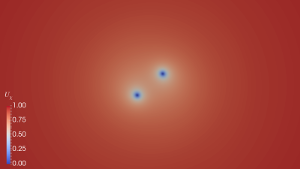
\includegraphics[width=0.9\textwidth]{figs/img_slice_chi_r1.png}
%			\caption{$q=1$}
%		\end{subfigure}
%		\begin{subfigure}{0.33\textwidth}
%			
\includegraphics[width=0.9\textwidth]{figs/img_slice_chi_r10.png}
%			\caption{$q=10$}
%		\end{subfigure}
%		\begin{subfigure}{0.33\textwidth}
%			
\includegraphics[width=0.9\textwidth]{figs/img_slice_chi_r100.png}
%			\caption{$q=100$}
%		\end{subfigure} \hfil
		\begin{subfigure}{0.33\textwidth}
			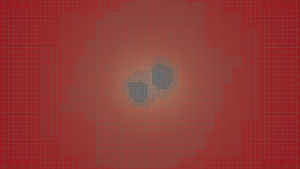
\includegraphics[width=0.9\textwidth]{figs/img_slice_level_r1.png}
			\caption{\large $q=1$}
		\end{subfigure}
		\begin{subfigure}{0.33\textwidth}
			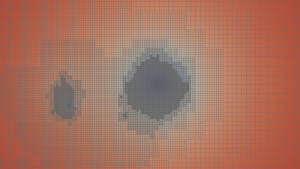
\includegraphics[width=0.9\textwidth]{figs/img_slice_level_r10.png}
			\caption{\large $q=10$}
		\end{subfigure}
		\begin{subfigure}{0.33\textwidth}
			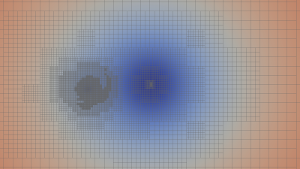
\includegraphics[width=0.9\textwidth]{figs/img_slice_level_r100.png}
			\caption{\large $q=100$}
		\end{subfigure}
	%	\caption{\small Time step snapshots of the binary black hole problem of black hole mass ratios $1, 10 \& 100$ where we in the top row we plot the \BSSN~variable $\chi$ in the lower row we plot the WAMR grids for each case at that specific instance. \label{fig:large_q}}
	\end{figure}
\end{textblock}


 \begin{textblock}{17}(0,6.5)
\Subhead{WAMR vs block/structured adaptivity}
\vspace{-0.2in}
\begin{textblock}{7}(0,0)
 \begin{figure}
	% 	\centering
	\begin{tikzpicture}
	\begin{axis}[
	%axis y line*=left,
	ylabel={grid points $\rightarrow$},%ymax=1,
	xlabel={mass ratio $\rightarrow$},legend pos=north west,
	width=7in, height=2.6in,grid=major,
	x tick label style={font=\small},
	]
	\addplot[thick,sq_b1,smooth,mark=*]  table [x={mr},y ={dof_zip}]{dat/stampede2/mr_et.dat};
	\addplot[thick,sq_r1,smooth,mark=diamond*]  table [x={mr},y ={dof_zip}]{dat/stampede2/mr_dendro.dat};
	\legend{\small ET(points), \small \dendro (points)}
	\end{axis}
	%	\begin{axis}[
	%	axis y line*=right,%ymax=1.5e6,
	%    axis x line=none,
	%  ylabel={grid points $\rightarrow$},
	%  width=0.45\textwidth, height=2in
	%	]
	%	\addplot[thick,sq_b3,smooth,mark=triangle*]  table [x={mr},y ={dof_zip}]{dat/stampede2/mr_et.dat};
	%	\addplot[thick,sq_r3,smooth,mark=square*]  table [x={mr},y ={dof_zip}]{dat/stampede2/mr_dendro.dat};
	%	\legend{ET(points), \dendro (points)}
	%	\end{axis}
	\end{tikzpicture} 
	
	%\pgfplotstabletypeset[columns={mass ratio,points(ET),time(ET)(s),points(XXXX),time(XXXX)(s)}]{dat/stampede2/mr_dendro_et.dat}
	%\caption{\label{fig:et_avec_adaptivity} \small Comparison between \et~ and \dendrogr\ for number of spatial points with increasing mass ratios. 
	%	Note that these are not from complete simulations and the size of the problem as well as the time per RK-step is likely to increase, but it illustrates the rate of increase for both approaches. Parameters for the above experiment generated such that total mass of black holes equals to $1$ and the separation distance is $32$ for all cases and \maxDepth~ is set in a way that the spatial discretization $dx<\frac{\min(m_1,m_2)}{16}$ where $m1,m2$ denotes the individual masses of black holes. 	
	%$RK$ time computed based average time to perform first $500$ time steps using $64$ cores on $2$ nodes in TACC's  \Stampede.
	%\hs{I have updated the caption. }
	%}
 	\vspace{-0.2in}
	\caption{\small Comparison between \et~ and \dendrogr\ for number of spatial points with increasing mass ratios. Note that these are not from complete simulations, but it illustrates the rate of increase for both approaches.}
\end{figure}	
\vspace{-0.5in}

\end{textblock}
\begin{textblock}{10}(8,0)
\begin{figure}
		\begin{tikzpicture}
\begin{semilogxaxis}[legend pos= north west,xlabel={$\leftarrow\ \ \ \alpha=\frac{\text{number of octants}}{\text{regular grid octants}}$},xmin=1e-8,xmax=1,ymax=800,
ylabel={time (s) $\rightarrow$},%grid=major,
width=10in,height=3.5in,legend pos=south west,x dir=reverse]
\addplot [blue,thin,mark=none,dashed,thick,smooth]table [x={gridRatio},y={rhs}]{dat/chpc/zipUnzip.dat};
\addplot [red,thin,mark=none,thick,smooth]table [x={gridRatio},y={total}]{dat/chpc/zipUnzip.dat};
%		\addplot[mark=none, black,dashed, samples=1] {525.36};
%		\addplot[mark=none, black, samples=1] {687.315};
%		\addplot coordinates {(1e-6,200) (1,200)};
\draw[dashed,thick,black] (axis cs:1e-8,525.36) --node[above right]{$RG$}  (axis cs:1,525.36);
\draw[thick,black] (axis cs:1e-8,687.315) -- node[above right]{\hspace{-0.6in}$RG+zip+unzip$}  (axis cs:1,687.315);
%		\draw[thick,black] (axis cs:3.72e-6,0) -- (axis cs:3.72e-6,800);

%\draw[black,fill=blue!20,opacity=0.5] (axis cs:3.72e-6,1e-3) rectangle (axis cs:3e-5,800) node[pos=.5] {$q=1$};

\draw[thick,decorate,decoration={brace,amplitude=0.2cm}]   (axis cs:3e-5,0) -- (axis cs:3.72e-6,1e-3);
\node at (axis cs:1e-5,75) {$q=1$};

%		\draw[black,fill=green!20,opacity=0.5] (axis cs:1.4e-6,1e-3) rectangle (axis cs:1.4e-9,800) node[pos=.3] {$q\geq 10$};
\draw[thick,decorate,decoration={brace,amplitude=0.2cm}]  (axis cs:1.4e-6,1e-3) -- (axis cs:1.4e-8,1e-3);
\node at (axis cs:1e-7,75) {$q\geq 10$};

%		\draw[thick,black] (axis cs:0.222,0) -- (axis cs:0.2222,800);\node[] at (axis cs:0.5,750) {\small $l=2$};
\draw[semithick, black, latex'-] (axis cs:0.0410, 0) -- (axis cs:0.0410,400);
\node at (axis cs:0.0410,425) {$L_3$};
\draw[semithick,black,latex'-] (axis cs:0.00683,0) -- (axis cs:0.00683,300);
\node at (axis cs:0.00683,325) {$L_4$};
\draw[semithick,black,latex'-] (axis cs:1.068e-3,0) -- (axis cs:1.068e-3,100);
\node at (axis cs:1.068e-3,125) {$L_5$};
%\legend{$rhs$,$rhs+zip+unzip$,$RG$,$RG+zip+unzip$}
\end{semilogxaxis}
\end{tikzpicture}
\vspace{-0.8in}
	\caption{\small Efficiency of zip/unzip operations with adaptivitve octrees.}
\end{figure}
\end{textblock}


 \end{textblock}	
	
				


\end{textblock}


\begin{textblock}{9}(10,5)
	{\color{DarkBlue}\hrule}\medskip
	\Head{Wavelet based adaptivity }
\vspace{-0.5in}
%	\begin{itemize}
%		\item We used wavelet based adaptive octrees generated by \dendro~ for our simulations. 
%	\end{itemize}
	
	
	%\Subhead{How Wavelets Work ?}
	\begin{figure}
		\centering
		\resizebox{7.5\TPHorizModule}{!}{
		\begin{tikzpicture}[yscale=-1.2]
		\begin{scope}
		\foreach \y in {0,1,2}
		\node[text width=1cm] at (-1,\y) {\small $V_\y$};
		\foreach \x in {0,4,8,12,16}
		\fill (\x,0) circle (0.1cm);
		
		\foreach \x in {0,2,4,6,8,10,12,14,16}
		\fill (\x,1) circle (0.1cm);		
		
		\foreach \x in {0,1,2,3,4,5,6,7,8,9,10,11,12,13,14,15,16}
		\fill (\x,2) circle (0.1cm);
		
		\node[text width=10cm,align=center] at (8,3.5) {\subcaption{$f(x) \in V_0 \subset V_1 \subset V_2$ \label{fig:w:a}} };
		\end{scope}
		
		\begin{scope}[yshift=5cm]
		
		\node[text width=1cm] at (-1,0) {\small $V_0$};
		
		\foreach \y in {1,2}
		\node[text width=1cm] at (-1,\y) {\small $W_\y$};
		\foreach \x in {0,4,8,12,16}
		\fill (\x,0) circle (0.1cm);
		
		\foreach \x in {2,6,10,14}
		\fill[red] (\x,1) circle (0.1cm);		
		
		\foreach \x in {1,3,5,7,9,11,13,15}
		\fill[blue] (\x,2) circle (0.1cm);
		
		\node[text width=15cm,align=center] at (8,3.5) {\subcaption{$W_{i,k}=|f(V_{i,k})-I(f(V{i-1,:}))|$ \label{fig:w:b}}};
		
		\end{scope}
		
		\begin{scope}[yshift=10cm]
		
		\node[text width=1cm] at (-1,0) {\small $V_0$};
		
		\foreach \y in {1,2}
		\node[text width=1cm] at (-1,\y) {\small $W_\y$};
		\foreach \x in {0,4,8,12,16}
		\fill (\x,0) circle (0.1cm);
		
		\foreach \x in {2,6,10,14}
		\fill[red] (\x,1) circle (0.1cm);		
		
		\draw[red] (6,1) circle (0.2cm);
		\draw[red] (10,1) circle (0.2cm);
		
		\foreach \x in {1,3,5,7,9,11,13,15}
		\fill[blue] (\x,2) circle (0.1cm);
		
		\draw[blue] (1,2) circle (0.2cm);
		\draw[blue] (3,2) circle (0.2cm);
		\draw[blue] (13,2) circle (0.2cm);
		\draw[blue] (15,2) circle (0.2cm);
		
		\node[text width=15cm,align=center] at (8,3.5) {\subcaption{$W_{i,k}\geq \epsilon \geq 0$ \label{fig:w:c}}};
		
		\end{scope}
		
		\begin{scope}[yshift=15cm]
		
		\node[text width=1cm] at (-1,0) {\small $V_0$};
		
		\foreach \y in {1,2}
		\node[text width=1cm] at (-1,\y) {\small $W_\y$};
		\foreach \x in {0,4,8,12,16}
		\fill (\x,0) circle (0.1cm);
		
		%	\foreach \x in {2,6,10,14}z
		%	\fill[red] (\x,1) circle (0.1cm);		
		
		\draw[red] (6,1) circle (0.2cm);
		\draw[red] (10,1) circle (0.2cm);
		
		%	\foreach \x in {1,3,5,7,9,11,13,15}
		%	\fill[blue] (\x,2) circle (0.1cm);
		
		\draw[blue] (1,2) circle (0.2cm);
		\draw[blue] (3,2) circle (0.2cm);
		\draw[blue] (13,2) circle (0.2cm);
		\draw[blue] (15,2) circle (0.2cm);
		
		\node[text width=15cm,align=center] at (8,3.5) {\subcaption{wavelet/sparse representation of $f(x)$ \label{fig:w:d}}};
		
		\end{scope}
		\end{tikzpicture}
		}
		\caption{For a given function $f:V\rightarrow \mathcal{R}$ let $V_i \subset V$ be the finite dimensional approximation of $f$ (see figure \ref{fig:w:a}). As number of nodes increases (i.e. going from $V_i$ to $V_{i+1}$) for each additional node introduced, we compute wavelet coefficients based on the absolute difference between $f(V_{i,k})$ and interpolated value from previous level $f(V_{i-1,:})$ (see figure \ref{fig:w:b}). In figure \ref{fig:w:c} shows the chosen nodes that violate specified wavelet tolerance $epsilon$ and these nodal wavelets
		are stored as the sparse/wavelet representation of function $f$ (see figure \ref{fig:w:d}).\label{fig:wavelets}}
	\end{figure}
	\vspace{0.1in}
	Example octrees generated based on Wavelet Adaptive Multi-Resolution (WAMR) for binary compact mergers.
	\begin{figure}
		\centering
		\resizebox{!}{2.5\TPHorizModule}{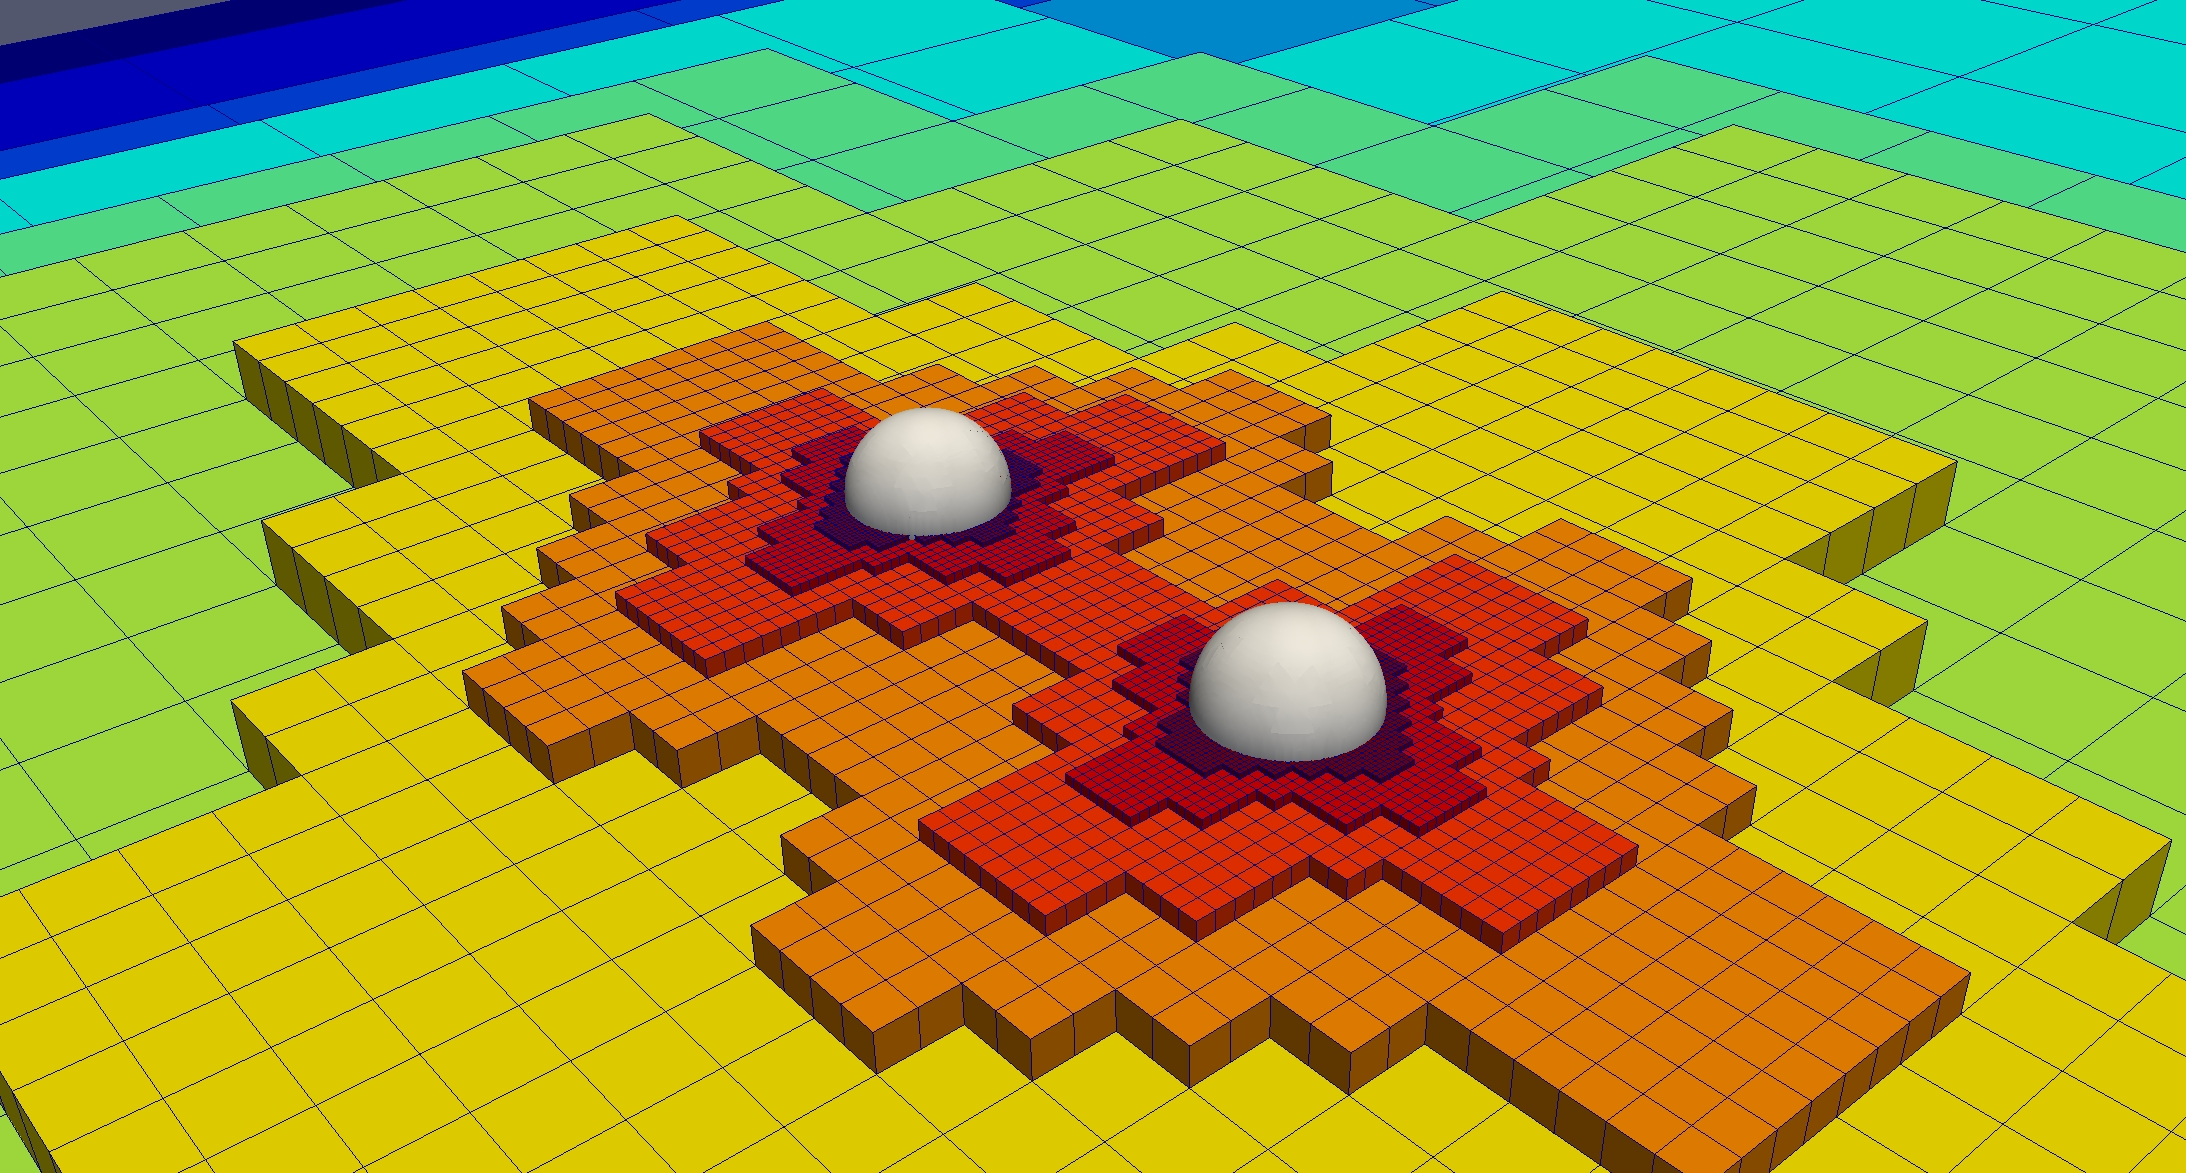
\includegraphics{figs/bh_img_1.jpg}}
		%		\hfill
		\resizebox{!}{2.5\TPHorizModule}{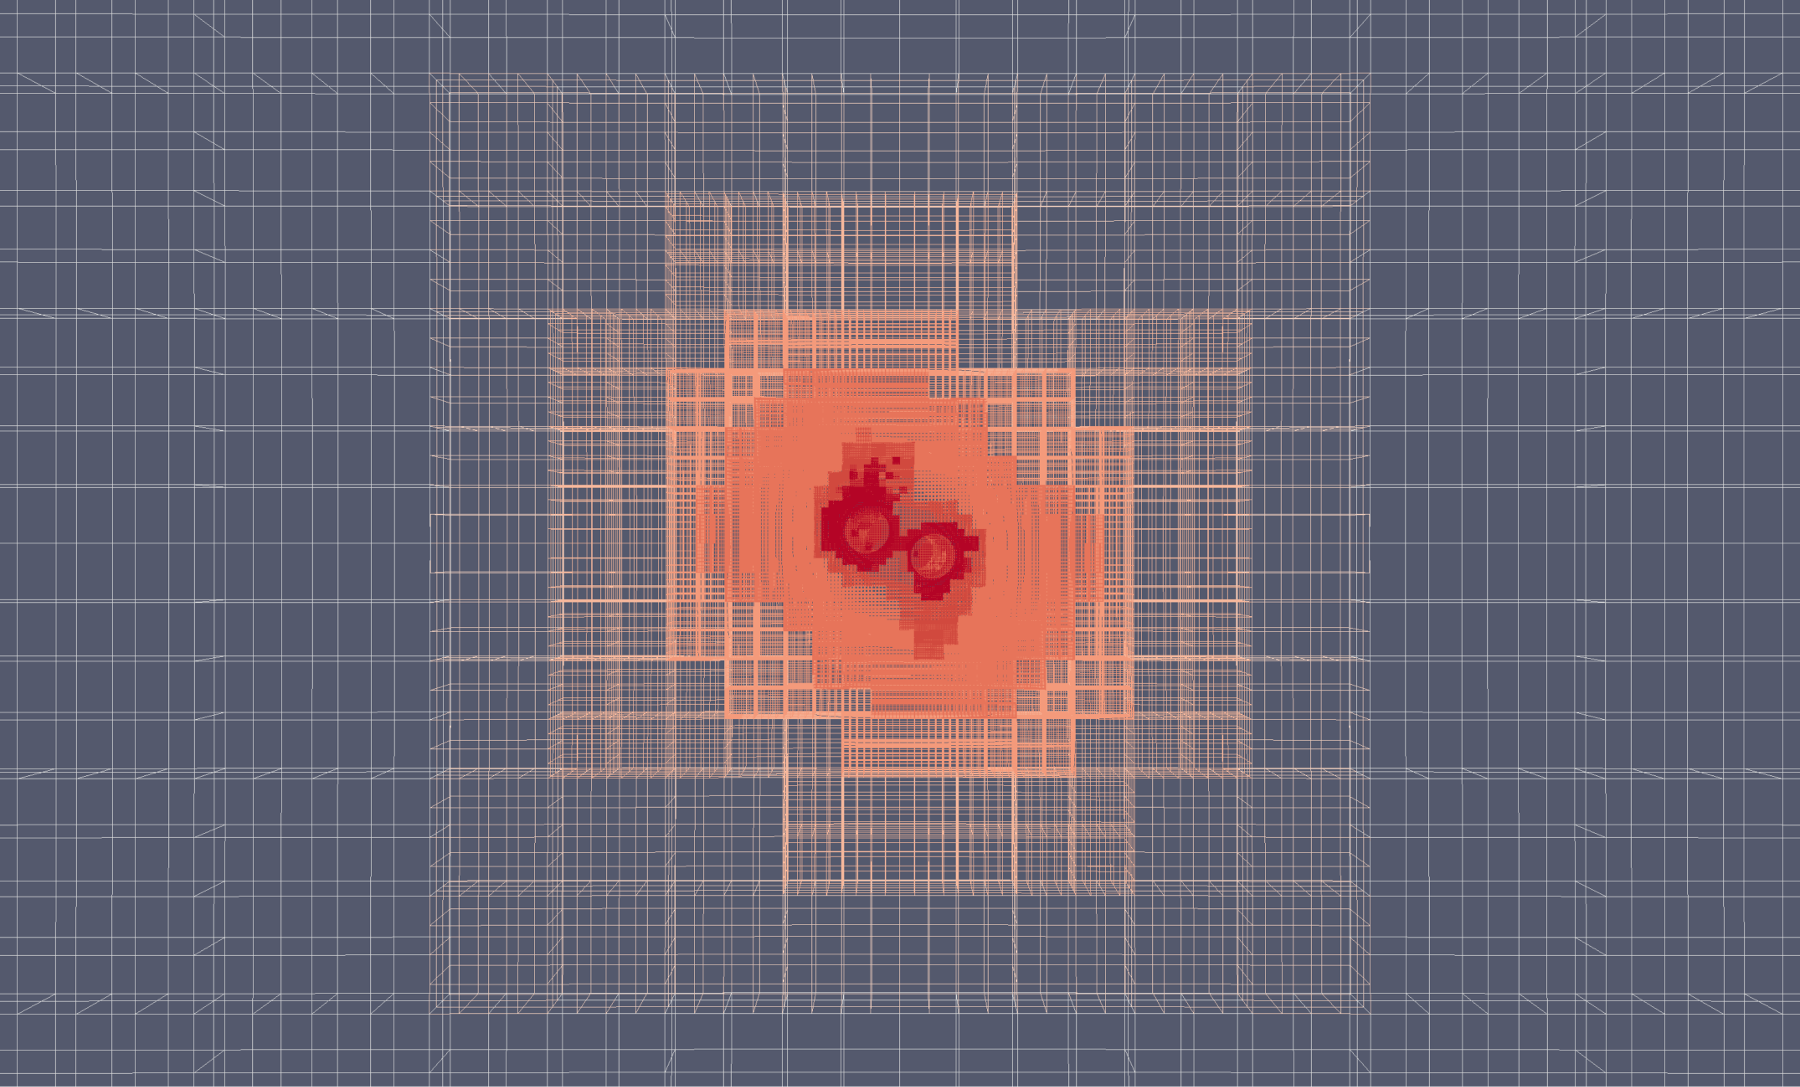
\includegraphics{figs/waveletgrids2.png}}
		\caption{\label{fig:bhole} ({\bf left}) A example of the adaptive mesh created by \dendro ~for the binary black-hole system. ({\bf right}) the hierarchical wavelet grids generated for the binary black hole system. }
	\end{figure}
	
	
\end{textblock}


%%%% ============ methods ======================
\begin{textblock}{32}(20,5)
	{\color{DarkBlue}\hrule}\medskip
	\Head{Methodology}

% \begin{textblock}{9}(0,0)
% \Subhead{Octree construction \& $2:1$ balancing}
% \begin{figure}

% 	\begin{subfigure}{0.33\textwidth}
% 		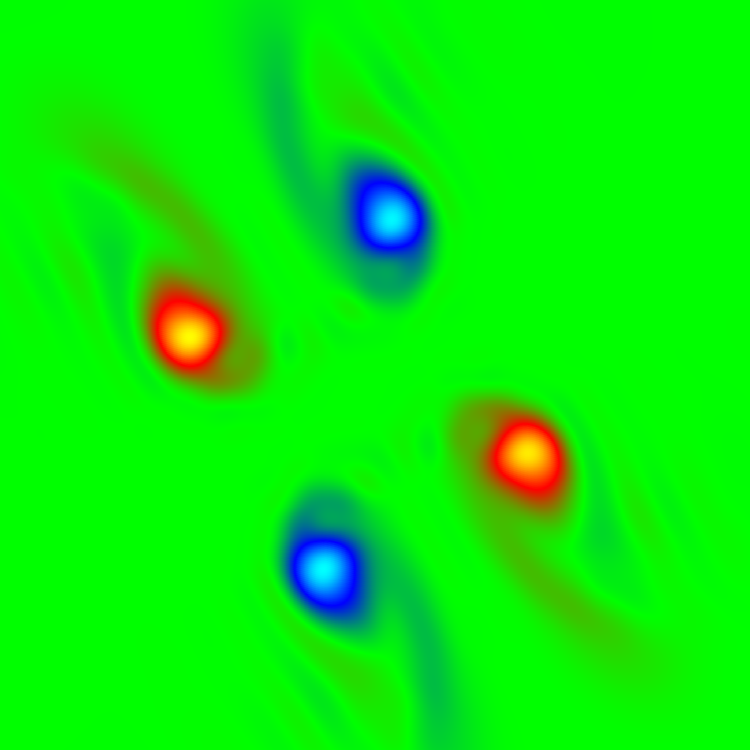
\includegraphics[width=0.9\textwidth]{figs/fn_val4.png}	
% 		\caption{$f(x), x\in \Omega$}
% 	\end{subfigure}
% 	\begin{subfigure}{0.33\textwidth}
% 		\resizebox{0.9\textwidth}{!}{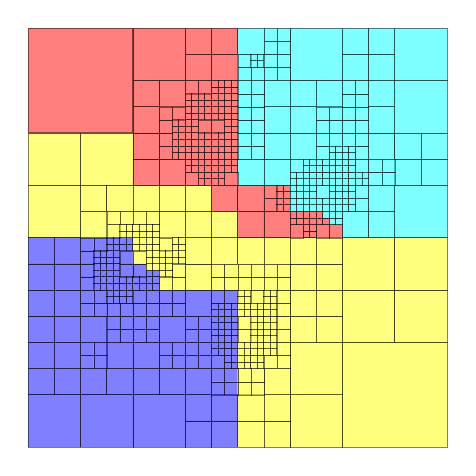
\begin{tikzpicture} [scale=3.8] {
  \begin{scope}[xshift=0cm,yshift=0cm,line width=0.5pt] {
  %\draw [black, opacity=0] (-1.1,-1.1) rectangle (1.1,1.1);  \definecolor{lineclr}{RGB}{0,0,0};
  \definecolor{fillclr1}{RGB}{0,0,255};
  \definecolor{fillclr2}{RGB}{255,255,0};
  \definecolor{fillclr3}{RGB}{255,0,0};
  \definecolor{fillclr4}{RGB}{0,255,255};
  \definecolor{fillclr5}{RGB}{0,255,0};
  \definecolor{fillclr6}{RGB}{255,0,255};
  \definecolor{fillclr7}{RGB}{255,255,255};
  \definecolor{fillclr8}{RGB}{0,0,0};
\draw[lineclr, line width=4*0.1pt, fill=fillclr2, opacity=0.5] (0.350000,-0.700000) -- (0.700000,-0.700000) -- (0.700000,-0.350000) -- (0.350000,-0.350000) -- (0.350000,-0.700000); 
\draw[lineclr, line width=4*0.1pt, fill=fillclr3, opacity=0.5] (-0.700000,0.350000) -- (-0.350000,0.350000) -- (-0.350000,0.700000) -- (-0.700000,0.700000) -- (-0.700000,0.350000); 
\draw[lineclr, line width=3*0.1pt, fill=fillclr1, opacity=0.5] (-0.700000,-0.700000) -- (-0.525000,-0.700000) -- (-0.525000,-0.525000) -- (-0.700000,-0.525000) -- (-0.700000,-0.700000); 
\draw[lineclr, line width=3*0.1pt, fill=fillclr1, opacity=0.5] (-0.525000,-0.700000) -- (-0.350000,-0.700000) -- (-0.350000,-0.525000) -- (-0.525000,-0.525000) -- (-0.525000,-0.700000); 
\draw[lineclr, line width=3*0.1pt, fill=fillclr1, opacity=0.5] (-0.350000,-0.700000) -- (-0.175000,-0.700000) -- (-0.175000,-0.525000) -- (-0.350000,-0.525000) -- (-0.350000,-0.700000); 
\draw[lineclr, line width=3*0.1pt, fill=fillclr2, opacity=0.5] (0.175000,-0.700000) -- (0.350000,-0.700000) -- (0.350000,-0.525000) -- (0.175000,-0.525000) -- (0.175000,-0.700000); 
\draw[lineclr, line width=3*0.1pt, fill=fillclr2, opacity=0.5] (0.175000,-0.525000) -- (0.350000,-0.525000) -- (0.350000,-0.350000) -- (0.175000,-0.350000) -- (0.175000,-0.525000); 
\draw[lineclr, line width=3*0.1pt, fill=fillclr2, opacity=0.5] (0.350000,-0.350000) -- (0.525000,-0.350000) -- (0.525000,-0.175000) -- (0.350000,-0.175000) -- (0.350000,-0.350000); 
\draw[lineclr, line width=3*0.1pt, fill=fillclr2, opacity=0.5] (0.525000,-0.350000) -- (0.700000,-0.350000) -- (0.700000,-0.175000) -- (0.525000,-0.175000) -- (0.525000,-0.350000); 
\draw[lineclr, line width=3*0.1pt, fill=fillclr2, opacity=0.5] (0.350000,-0.175000) -- (0.525000,-0.175000) -- (0.525000,0.000000) -- (0.350000,0.000000) -- (0.350000,-0.175000); 
\draw[lineclr, line width=3*0.1pt, fill=fillclr2, opacity=0.5] (0.525000,-0.175000) -- (0.700000,-0.175000) -- (0.700000,0.000000) -- (0.525000,0.000000) -- (0.525000,-0.175000); 
\draw[lineclr, line width=3*0.1pt, fill=fillclr2, opacity=0.5] (-0.700000,0.000000) -- (-0.525000,0.000000) -- (-0.525000,0.175000) -- (-0.700000,0.175000) -- (-0.700000,0.000000); 
\draw[lineclr, line width=3*0.1pt, fill=fillclr4, opacity=0.5] (0.525000,0.000000) -- (0.700000,0.000000) -- (0.700000,0.175000) -- (0.525000,0.175000) -- (0.525000,0.000000); 
\draw[lineclr, line width=3*0.1pt, fill=fillclr2, opacity=0.5] (-0.700000,0.175000) -- (-0.525000,0.175000) -- (-0.525000,0.350000) -- (-0.700000,0.350000) -- (-0.700000,0.175000); 
\draw[lineclr, line width=3*0.1pt, fill=fillclr2, opacity=0.5] (-0.525000,0.175000) -- (-0.350000,0.175000) -- (-0.350000,0.350000) -- (-0.525000,0.350000) -- (-0.525000,0.175000); 
\draw[lineclr, line width=3*0.1pt, fill=fillclr4, opacity=0.5] (0.525000,0.350000) -- (0.700000,0.350000) -- (0.700000,0.525000) -- (0.525000,0.525000) -- (0.525000,0.350000); 
\draw[lineclr, line width=3*0.1pt, fill=fillclr3, opacity=0.5] (-0.350000,0.525000) -- (-0.175000,0.525000) -- (-0.175000,0.700000) -- (-0.350000,0.700000) -- (-0.350000,0.525000); 
\draw[lineclr, line width=3*0.1pt, fill=fillclr4, opacity=0.5] (0.175000,0.525000) -- (0.350000,0.525000) -- (0.350000,0.700000) -- (0.175000,0.700000) -- (0.175000,0.525000); 
\draw[lineclr, line width=3*0.1pt, fill=fillclr4, opacity=0.5] (0.525000,0.525000) -- (0.700000,0.525000) -- (0.700000,0.700000) -- (0.525000,0.700000) -- (0.525000,0.525000); 
\draw[lineclr, line width=2*0.1pt, fill=fillclr1, opacity=0.5] (-0.175000,-0.700000) -- (-0.087500,-0.700000) -- (-0.087500,-0.612500) -- (-0.175000,-0.612500) -- (-0.175000,-0.700000); 
\draw[lineclr, line width=2*0.1pt, fill=fillclr1, opacity=0.5] (-0.087500,-0.700000) -- (0.000000,-0.700000) -- (0.000000,-0.612500) -- (-0.087500,-0.612500) -- (-0.087500,-0.700000); 
\draw[lineclr, line width=2*0.1pt, fill=fillclr2, opacity=0.5] (0.000000,-0.700000) -- (0.087500,-0.700000) -- (0.087500,-0.612500) -- (0.000000,-0.612500) -- (0.000000,-0.700000); 
\draw[lineclr, line width=2*0.1pt, fill=fillclr2, opacity=0.5] (0.087500,-0.700000) -- (0.175000,-0.700000) -- (0.175000,-0.612500) -- (0.087500,-0.612500) -- (0.087500,-0.700000); 
\draw[lineclr, line width=2*0.1pt, fill=fillclr1, opacity=0.5] (-0.175000,-0.612500) -- (-0.087500,-0.612500) -- (-0.087500,-0.525000) -- (-0.175000,-0.525000) -- (-0.175000,-0.612500); 
\draw[lineclr, line width=2*0.1pt, fill=fillclr1, opacity=0.5] (-0.087500,-0.612500) -- (0.000000,-0.612500) -- (0.000000,-0.525000) -- (-0.087500,-0.525000) -- (-0.087500,-0.612500); 
\draw[lineclr, line width=2*0.1pt, fill=fillclr2, opacity=0.5] (0.000000,-0.612500) -- (0.087500,-0.612500) -- (0.087500,-0.525000) -- (0.000000,-0.525000) -- (0.000000,-0.612500); 
\draw[lineclr, line width=2*0.1pt, fill=fillclr2, opacity=0.5] (0.087500,-0.612500) -- (0.175000,-0.612500) -- (0.175000,-0.525000) -- (0.087500,-0.525000) -- (0.087500,-0.612500); 
\draw[lineclr, line width=2*0.1pt, fill=fillclr1, opacity=0.5] (-0.700000,-0.525000) -- (-0.612500,-0.525000) -- (-0.612500,-0.437500) -- (-0.700000,-0.437500) -- (-0.700000,-0.525000); 
\draw[lineclr, line width=2*0.1pt, fill=fillclr1, opacity=0.5] (-0.612500,-0.525000) -- (-0.525000,-0.525000) -- (-0.525000,-0.437500) -- (-0.612500,-0.437500) -- (-0.612500,-0.525000); 
\draw[lineclr, line width=2*0.1pt, fill=fillclr1, opacity=0.5] (-0.525000,-0.525000) -- (-0.437500,-0.525000) -- (-0.437500,-0.437500) -- (-0.525000,-0.437500) -- (-0.525000,-0.525000); 
\draw[lineclr, line width=2*0.1pt, fill=fillclr1, opacity=0.5] (-0.437500,-0.525000) -- (-0.350000,-0.525000) -- (-0.350000,-0.437500) -- (-0.437500,-0.437500) -- (-0.437500,-0.525000); 
\draw[lineclr, line width=2*0.1pt, fill=fillclr1, opacity=0.5] (-0.350000,-0.525000) -- (-0.262500,-0.525000) -- (-0.262500,-0.437500) -- (-0.350000,-0.437500) -- (-0.350000,-0.525000); 
\draw[lineclr, line width=2*0.1pt, fill=fillclr1, opacity=0.5] (-0.262500,-0.525000) -- (-0.175000,-0.525000) -- (-0.175000,-0.437500) -- (-0.262500,-0.437500) -- (-0.262500,-0.525000); 
\draw[lineclr, line width=2*0.1pt, fill=fillclr1, opacity=0.5] (-0.175000,-0.525000) -- (-0.087500,-0.525000) -- (-0.087500,-0.437500) -- (-0.175000,-0.437500) -- (-0.175000,-0.525000); 
\draw[lineclr, line width=2*0.1pt, fill=fillclr2, opacity=0.5] (0.087500,-0.525000) -- (0.175000,-0.525000) -- (0.175000,-0.437500) -- (0.087500,-0.437500) -- (0.087500,-0.525000); 
\draw[lineclr, line width=2*0.1pt, fill=fillclr1, opacity=0.5] (-0.700000,-0.437500) -- (-0.612500,-0.437500) -- (-0.612500,-0.350000) -- (-0.700000,-0.350000) -- (-0.700000,-0.437500); 
\draw[lineclr, line width=2*0.1pt, fill=fillclr1, opacity=0.5] (-0.612500,-0.437500) -- (-0.525000,-0.437500) -- (-0.525000,-0.350000) -- (-0.612500,-0.350000) -- (-0.612500,-0.437500); 
\draw[lineclr, line width=2*0.1pt, fill=fillclr1, opacity=0.5] (-0.437500,-0.437500) -- (-0.350000,-0.437500) -- (-0.350000,-0.350000) -- (-0.437500,-0.350000) -- (-0.437500,-0.437500); 
\draw[lineclr, line width=2*0.1pt, fill=fillclr1, opacity=0.5] (-0.350000,-0.437500) -- (-0.262500,-0.437500) -- (-0.262500,-0.350000) -- (-0.350000,-0.350000) -- (-0.350000,-0.437500); 
\draw[lineclr, line width=2*0.1pt, fill=fillclr1, opacity=0.5] (-0.700000,-0.350000) -- (-0.612500,-0.350000) -- (-0.612500,-0.262500) -- (-0.700000,-0.262500) -- (-0.700000,-0.350000); 
\draw[lineclr, line width=2*0.1pt, fill=fillclr1, opacity=0.5] (-0.612500,-0.350000) -- (-0.525000,-0.350000) -- (-0.525000,-0.262500) -- (-0.612500,-0.262500) -- (-0.612500,-0.350000); 
\draw[lineclr, line width=2*0.1pt, fill=fillclr1, opacity=0.5] (-0.525000,-0.350000) -- (-0.437500,-0.350000) -- (-0.437500,-0.262500) -- (-0.525000,-0.262500) -- (-0.525000,-0.350000); 
\draw[lineclr, line width=2*0.1pt, fill=fillclr1, opacity=0.5] (-0.262500,-0.350000) -- (-0.175000,-0.350000) -- (-0.175000,-0.262500) -- (-0.262500,-0.262500) -- (-0.262500,-0.350000); 
\draw[lineclr, line width=2*0.1pt, fill=fillclr2, opacity=0.5] (0.175000,-0.350000) -- (0.262500,-0.350000) -- (0.262500,-0.262500) -- (0.175000,-0.262500) -- (0.175000,-0.350000); 
\draw[lineclr, line width=2*0.1pt, fill=fillclr2, opacity=0.5] (0.262500,-0.350000) -- (0.350000,-0.350000) -- (0.350000,-0.262500) -- (0.262500,-0.262500) -- (0.262500,-0.350000); 
\draw[lineclr, line width=2*0.1pt, fill=fillclr1, opacity=0.5] (-0.700000,-0.262500) -- (-0.612500,-0.262500) -- (-0.612500,-0.175000) -- (-0.700000,-0.175000) -- (-0.700000,-0.262500); 
\draw[lineclr, line width=2*0.1pt, fill=fillclr1, opacity=0.5] (-0.612500,-0.262500) -- (-0.525000,-0.262500) -- (-0.525000,-0.175000) -- (-0.612500,-0.175000) -- (-0.612500,-0.262500); 
\draw[lineclr, line width=2*0.1pt, fill=fillclr1, opacity=0.5] (-0.175000,-0.262500) -- (-0.087500,-0.262500) -- (-0.087500,-0.175000) -- (-0.175000,-0.175000) -- (-0.175000,-0.262500); 
\draw[lineclr, line width=2*0.1pt, fill=fillclr2, opacity=0.5] (0.175000,-0.262500) -- (0.262500,-0.262500) -- (0.262500,-0.175000) -- (0.175000,-0.175000) -- (0.175000,-0.262500); 
\draw[lineclr, line width=2*0.1pt, fill=fillclr2, opacity=0.5] (0.262500,-0.262500) -- (0.350000,-0.262500) -- (0.350000,-0.175000) -- (0.262500,-0.175000) -- (0.262500,-0.262500); 
\draw[lineclr, line width=2*0.1pt, fill=fillclr1, opacity=0.5] (-0.700000,-0.175000) -- (-0.612500,-0.175000) -- (-0.612500,-0.087500) -- (-0.700000,-0.087500) -- (-0.700000,-0.175000); 
\draw[lineclr, line width=2*0.1pt, fill=fillclr1, opacity=0.5] (-0.612500,-0.175000) -- (-0.525000,-0.175000) -- (-0.525000,-0.087500) -- (-0.612500,-0.087500) -- (-0.612500,-0.175000); 
\draw[lineclr, line width=2*0.1pt, fill=fillclr2, opacity=0.5] (-0.175000,-0.175000) -- (-0.087500,-0.175000) -- (-0.087500,-0.087500) -- (-0.175000,-0.087500) -- (-0.175000,-0.175000); 
\draw[lineclr, line width=2*0.1pt, fill=fillclr2, opacity=0.5] (0.175000,-0.175000) -- (0.262500,-0.175000) -- (0.262500,-0.087500) -- (0.175000,-0.087500) -- (0.175000,-0.175000); 
\draw[lineclr, line width=2*0.1pt, fill=fillclr2, opacity=0.5] (0.262500,-0.175000) -- (0.350000,-0.175000) -- (0.350000,-0.087500) -- (0.262500,-0.087500) -- (0.262500,-0.175000); 
\draw[lineclr, line width=2*0.1pt, fill=fillclr1, opacity=0.5] (-0.700000,-0.087500) -- (-0.612500,-0.087500) -- (-0.612500,0.000000) -- (-0.700000,0.000000) -- (-0.700000,-0.087500); 
\draw[lineclr, line width=2*0.1pt, fill=fillclr1, opacity=0.5] (-0.612500,-0.087500) -- (-0.525000,-0.087500) -- (-0.525000,0.000000) -- (-0.612500,0.000000) -- (-0.612500,-0.087500); 
\draw[lineclr, line width=2*0.1pt, fill=fillclr2, opacity=0.5] (-0.175000,-0.087500) -- (-0.087500,-0.087500) -- (-0.087500,0.000000) -- (-0.175000,0.000000) -- (-0.175000,-0.087500); 
\draw[lineclr, line width=2*0.1pt, fill=fillclr2, opacity=0.5] (-0.087500,-0.087500) -- (0.000000,-0.087500) -- (0.000000,0.000000) -- (-0.087500,0.000000) -- (-0.087500,-0.087500); 
\draw[lineclr, line width=2*0.1pt, fill=fillclr2, opacity=0.5] (0.000000,-0.087500) -- (0.087500,-0.087500) -- (0.087500,0.000000) -- (0.000000,0.000000) -- (0.000000,-0.087500); 
\draw[lineclr, line width=2*0.1pt, fill=fillclr2, opacity=0.5] (0.087500,-0.087500) -- (0.175000,-0.087500) -- (0.175000,0.000000) -- (0.087500,0.000000) -- (0.087500,-0.087500); 
\draw[lineclr, line width=2*0.1pt, fill=fillclr2, opacity=0.5] (0.175000,-0.087500) -- (0.262500,-0.087500) -- (0.262500,0.000000) -- (0.175000,0.000000) -- (0.175000,-0.087500); 
\draw[lineclr, line width=2*0.1pt, fill=fillclr2, opacity=0.5] (0.262500,-0.087500) -- (0.350000,-0.087500) -- (0.350000,0.000000) -- (0.262500,0.000000) -- (0.262500,-0.087500); 
\draw[lineclr, line width=2*0.1pt, fill=fillclr2, opacity=0.5] (-0.525000,0.000000) -- (-0.437500,0.000000) -- (-0.437500,0.087500) -- (-0.525000,0.087500) -- (-0.525000,0.000000); 
\draw[lineclr, line width=2*0.1pt, fill=fillclr2, opacity=0.5] (-0.262500,0.000000) -- (-0.175000,0.000000) -- (-0.175000,0.087500) -- (-0.262500,0.087500) -- (-0.262500,0.000000); 
\draw[lineclr, line width=2*0.1pt, fill=fillclr2, opacity=0.5] (-0.175000,0.000000) -- (-0.087500,0.000000) -- (-0.087500,0.087500) -- (-0.175000,0.087500) -- (-0.175000,0.000000); 
\draw[lineclr, line width=2*0.1pt, fill=fillclr2, opacity=0.5] (-0.087500,0.000000) -- (0.000000,0.000000) -- (0.000000,0.087500) -- (-0.087500,0.087500) -- (-0.087500,0.000000); 
\draw[lineclr, line width=2*0.1pt, fill=fillclr3, opacity=0.5] (0.000000,0.000000) -- (0.087500,0.000000) -- (0.087500,0.087500) -- (0.000000,0.087500) -- (0.000000,0.000000); 
\draw[lineclr, line width=2*0.1pt, fill=fillclr3, opacity=0.5] (0.087500,0.000000) -- (0.175000,0.000000) -- (0.175000,0.087500) -- (0.087500,0.087500) -- (0.087500,0.000000); 
\draw[lineclr, line width=2*0.1pt, fill=fillclr4, opacity=0.5] (0.350000,0.000000) -- (0.437500,0.000000) -- (0.437500,0.087500) -- (0.350000,0.087500) -- (0.350000,0.000000); 
\draw[lineclr, line width=2*0.1pt, fill=fillclr4, opacity=0.5] (0.437500,0.000000) -- (0.525000,0.000000) -- (0.525000,0.087500) -- (0.437500,0.087500) -- (0.437500,0.000000); 
\draw[lineclr, line width=2*0.1pt, fill=fillclr2, opacity=0.5] (-0.525000,0.087500) -- (-0.437500,0.087500) -- (-0.437500,0.175000) -- (-0.525000,0.175000) -- (-0.525000,0.087500); 
\draw[lineclr, line width=2*0.1pt, fill=fillclr2, opacity=0.5] (-0.437500,0.087500) -- (-0.350000,0.087500) -- (-0.350000,0.175000) -- (-0.437500,0.175000) -- (-0.437500,0.087500); 
\draw[lineclr, line width=2*0.1pt, fill=fillclr2, opacity=0.5] (-0.350000,0.087500) -- (-0.262500,0.087500) -- (-0.262500,0.175000) -- (-0.350000,0.175000) -- (-0.350000,0.087500); 
\draw[lineclr, line width=2*0.1pt, fill=fillclr2, opacity=0.5] (-0.262500,0.087500) -- (-0.175000,0.087500) -- (-0.175000,0.175000) -- (-0.262500,0.175000) -- (-0.262500,0.087500); 
\draw[lineclr, line width=2*0.1pt, fill=fillclr2, opacity=0.5] (-0.175000,0.087500) -- (-0.087500,0.087500) -- (-0.087500,0.175000) -- (-0.175000,0.175000) -- (-0.175000,0.087500); 
\draw[lineclr, line width=2*0.1pt, fill=fillclr3, opacity=0.5] (-0.087500,0.087500) -- (0.000000,0.087500) -- (0.000000,0.175000) -- (-0.087500,0.175000) -- (-0.087500,0.087500); 
\draw[lineclr, line width=2*0.1pt, fill=fillclr3, opacity=0.5] (0.000000,0.087500) -- (0.087500,0.087500) -- (0.087500,0.175000) -- (0.000000,0.175000) -- (0.000000,0.087500); 
\draw[lineclr, line width=2*0.1pt, fill=fillclr4, opacity=0.5] (0.437500,0.087500) -- (0.525000,0.087500) -- (0.525000,0.175000) -- (0.437500,0.175000) -- (0.437500,0.087500); 
\draw[lineclr, line width=2*0.1pt, fill=fillclr3, opacity=0.5] (-0.350000,0.175000) -- (-0.262500,0.175000) -- (-0.262500,0.262500) -- (-0.350000,0.262500) -- (-0.350000,0.175000); 
\draw[lineclr, line width=2*0.1pt, fill=fillclr3, opacity=0.5] (-0.262500,0.175000) -- (-0.175000,0.175000) -- (-0.175000,0.262500) -- (-0.262500,0.262500) -- (-0.262500,0.175000); 
\draw[lineclr, line width=2*0.1pt, fill=fillclr4, opacity=0.5] (0.000000,0.175000) -- (0.087500,0.175000) -- (0.087500,0.262500) -- (0.000000,0.262500) -- (0.000000,0.175000); 
\draw[lineclr, line width=2*0.1pt, fill=fillclr4, opacity=0.5] (0.087500,0.175000) -- (0.175000,0.175000) -- (0.175000,0.262500) -- (0.087500,0.262500) -- (0.087500,0.175000); 
\draw[lineclr, line width=2*0.1pt, fill=fillclr4, opacity=0.5] (0.525000,0.175000) -- (0.612500,0.175000) -- (0.612500,0.262500) -- (0.525000,0.262500) -- (0.525000,0.175000); 
\draw[lineclr, line width=2*0.1pt, fill=fillclr4, opacity=0.5] (0.612500,0.175000) -- (0.700000,0.175000) -- (0.700000,0.262500) -- (0.612500,0.262500) -- (0.612500,0.175000); 
\draw[lineclr, line width=2*0.1pt, fill=fillclr3, opacity=0.5] (-0.350000,0.262500) -- (-0.262500,0.262500) -- (-0.262500,0.350000) -- (-0.350000,0.350000) -- (-0.350000,0.262500); 
\draw[lineclr, line width=2*0.1pt, fill=fillclr4, opacity=0.5] (0.087500,0.262500) -- (0.175000,0.262500) -- (0.175000,0.350000) -- (0.087500,0.350000) -- (0.087500,0.262500); 
\draw[lineclr, line width=2*0.1pt, fill=fillclr4, opacity=0.5] (0.175000,0.262500) -- (0.262500,0.262500) -- (0.262500,0.350000) -- (0.175000,0.350000) -- (0.175000,0.262500); 
\draw[lineclr, line width=2*0.1pt, fill=fillclr4, opacity=0.5] (0.437500,0.262500) -- (0.525000,0.262500) -- (0.525000,0.350000) -- (0.437500,0.350000) -- (0.437500,0.262500); 
\draw[lineclr, line width=2*0.1pt, fill=fillclr4, opacity=0.5] (0.525000,0.262500) -- (0.612500,0.262500) -- (0.612500,0.350000) -- (0.525000,0.350000) -- (0.525000,0.262500); 
\draw[lineclr, line width=2*0.1pt, fill=fillclr4, opacity=0.5] (0.612500,0.262500) -- (0.700000,0.262500) -- (0.700000,0.350000) -- (0.612500,0.350000) -- (0.612500,0.262500); 
\draw[lineclr, line width=2*0.1pt, fill=fillclr3, opacity=0.5] (-0.350000,0.350000) -- (-0.262500,0.350000) -- (-0.262500,0.437500) -- (-0.350000,0.437500) -- (-0.350000,0.350000); 
\draw[lineclr, line width=2*0.1pt, fill=fillclr4, opacity=0.5] (0.087500,0.350000) -- (0.175000,0.350000) -- (0.175000,0.437500) -- (0.087500,0.437500) -- (0.087500,0.350000); 
\draw[lineclr, line width=2*0.1pt, fill=fillclr4, opacity=0.5] (0.175000,0.350000) -- (0.262500,0.350000) -- (0.262500,0.437500) -- (0.175000,0.437500) -- (0.175000,0.350000); 
\draw[lineclr, line width=2*0.1pt, fill=fillclr4, opacity=0.5] (0.437500,0.350000) -- (0.525000,0.350000) -- (0.525000,0.437500) -- (0.437500,0.437500) -- (0.437500,0.350000); 
\draw[lineclr, line width=2*0.1pt, fill=fillclr3, opacity=0.5] (-0.350000,0.437500) -- (-0.262500,0.437500) -- (-0.262500,0.525000) -- (-0.350000,0.525000) -- (-0.350000,0.437500); 
\draw[lineclr, line width=2*0.1pt, fill=fillclr3, opacity=0.5] (-0.262500,0.437500) -- (-0.175000,0.437500) -- (-0.175000,0.525000) -- (-0.262500,0.525000) -- (-0.262500,0.437500); 
\draw[lineclr, line width=2*0.1pt, fill=fillclr4, opacity=0.5] (0.087500,0.437500) -- (0.175000,0.437500) -- (0.175000,0.525000) -- (0.087500,0.525000) -- (0.087500,0.437500); 
\draw[lineclr, line width=2*0.1pt, fill=fillclr4, opacity=0.5] (0.175000,0.437500) -- (0.262500,0.437500) -- (0.262500,0.525000) -- (0.175000,0.525000) -- (0.175000,0.437500); 
\draw[lineclr, line width=2*0.1pt, fill=fillclr4, opacity=0.5] (0.262500,0.437500) -- (0.350000,0.437500) -- (0.350000,0.525000) -- (0.262500,0.525000) -- (0.262500,0.437500); 
\draw[lineclr, line width=2*0.1pt, fill=fillclr4, opacity=0.5] (0.437500,0.437500) -- (0.525000,0.437500) -- (0.525000,0.525000) -- (0.437500,0.525000) -- (0.437500,0.437500); 
\draw[lineclr, line width=2*0.1pt, fill=fillclr3, opacity=0.5] (-0.175000,0.525000) -- (-0.087500,0.525000) -- (-0.087500,0.612500) -- (-0.175000,0.612500) -- (-0.175000,0.525000); 
\draw[lineclr, line width=2*0.1pt, fill=fillclr3, opacity=0.5] (-0.087500,0.525000) -- (0.000000,0.525000) -- (0.000000,0.612500) -- (-0.087500,0.612500) -- (-0.087500,0.525000); 
\draw[lineclr, line width=2*0.1pt, fill=fillclr4, opacity=0.5] (0.350000,0.525000) -- (0.437500,0.525000) -- (0.437500,0.612500) -- (0.350000,0.612500) -- (0.350000,0.525000); 
\draw[lineclr, line width=2*0.1pt, fill=fillclr4, opacity=0.5] (0.437500,0.525000) -- (0.525000,0.525000) -- (0.525000,0.612500) -- (0.437500,0.612500) -- (0.437500,0.525000); 
\draw[lineclr, line width=2*0.1pt, fill=fillclr3, opacity=0.5] (-0.175000,0.612500) -- (-0.087500,0.612500) -- (-0.087500,0.700000) -- (-0.175000,0.700000) -- (-0.175000,0.612500); 
\draw[lineclr, line width=2*0.1pt, fill=fillclr3, opacity=0.5] (-0.087500,0.612500) -- (0.000000,0.612500) -- (0.000000,0.700000) -- (-0.087500,0.700000) -- (-0.087500,0.612500); 
\draw[lineclr, line width=2*0.1pt, fill=fillclr4, opacity=0.5] (0.000000,0.612500) -- (0.087500,0.612500) -- (0.087500,0.700000) -- (0.000000,0.700000) -- (0.000000,0.612500); 
\draw[lineclr, line width=2*0.1pt, fill=fillclr4, opacity=0.5] (0.350000,0.612500) -- (0.437500,0.612500) -- (0.437500,0.700000) -- (0.350000,0.700000) -- (0.350000,0.612500); 
\draw[lineclr, line width=2*0.1pt, fill=fillclr4, opacity=0.5] (0.437500,0.612500) -- (0.525000,0.612500) -- (0.525000,0.700000) -- (0.437500,0.700000) -- (0.437500,0.612500); 
\draw[lineclr, line width=1*0.1pt, fill=fillclr1, opacity=0.5] (-0.087500,-0.525000) -- (-0.043750,-0.525000) -- (-0.043750,-0.481250) -- (-0.087500,-0.481250) -- (-0.087500,-0.525000); 
\draw[lineclr, line width=1*0.1pt, fill=fillclr1, opacity=0.5] (-0.043750,-0.525000) -- (0.000000,-0.525000) -- (0.000000,-0.481250) -- (-0.043750,-0.481250) -- (-0.043750,-0.525000); 
\draw[lineclr, line width=1*0.1pt, fill=fillclr2, opacity=0.5] (0.000000,-0.525000) -- (0.043750,-0.525000) -- (0.043750,-0.481250) -- (0.000000,-0.481250) -- (0.000000,-0.525000); 
\draw[lineclr, line width=1*0.1pt, fill=fillclr2, opacity=0.5] (0.043750,-0.525000) -- (0.087500,-0.525000) -- (0.087500,-0.481250) -- (0.043750,-0.481250) -- (0.043750,-0.525000); 
\draw[lineclr, line width=1*0.1pt, fill=fillclr1, opacity=0.5] (-0.087500,-0.481250) -- (-0.043750,-0.481250) -- (-0.043750,-0.437500) -- (-0.087500,-0.437500) -- (-0.087500,-0.481250); 
\draw[lineclr, line width=1*0.1pt, fill=fillclr1, opacity=0.5] (-0.043750,-0.481250) -- (0.000000,-0.481250) -- (0.000000,-0.437500) -- (-0.043750,-0.437500) -- (-0.043750,-0.481250); 
\draw[lineclr, line width=1*0.1pt, fill=fillclr2, opacity=0.5] (0.000000,-0.481250) -- (0.043750,-0.481250) -- (0.043750,-0.437500) -- (0.000000,-0.437500) -- (0.000000,-0.481250); 
\draw[lineclr, line width=1*0.1pt, fill=fillclr2, opacity=0.5] (0.043750,-0.481250) -- (0.087500,-0.481250) -- (0.087500,-0.437500) -- (0.043750,-0.437500) -- (0.043750,-0.481250); 
\draw[lineclr, line width=1*0.1pt, fill=fillclr1, opacity=0.5] (-0.525000,-0.437500) -- (-0.481250,-0.437500) -- (-0.481250,-0.393750) -- (-0.525000,-0.393750) -- (-0.525000,-0.437500); 
\draw[lineclr, line width=1*0.1pt, fill=fillclr1, opacity=0.5] (-0.481250,-0.437500) -- (-0.437500,-0.437500) -- (-0.437500,-0.393750) -- (-0.481250,-0.393750) -- (-0.481250,-0.437500); 
\draw[lineclr, line width=1*0.1pt, fill=fillclr1, opacity=0.5] (-0.262500,-0.437500) -- (-0.218750,-0.437500) -- (-0.218750,-0.393750) -- (-0.262500,-0.393750) -- (-0.262500,-0.437500); 
\draw[lineclr, line width=1*0.1pt, fill=fillclr1, opacity=0.5] (-0.218750,-0.437500) -- (-0.175000,-0.437500) -- (-0.175000,-0.393750) -- (-0.218750,-0.393750) -- (-0.218750,-0.437500); 
\draw[lineclr, line width=1*0.1pt, fill=fillclr1, opacity=0.5] (-0.175000,-0.437500) -- (-0.131250,-0.437500) -- (-0.131250,-0.393750) -- (-0.175000,-0.393750) -- (-0.175000,-0.437500); 
\draw[lineclr, line width=1*0.1pt, fill=fillclr1, opacity=0.5] (-0.131250,-0.437500) -- (-0.087500,-0.437500) -- (-0.087500,-0.393750) -- (-0.131250,-0.393750) -- (-0.131250,-0.437500); 
\draw[lineclr, line width=1*0.1pt, fill=fillclr1, opacity=0.5] (-0.087500,-0.437500) -- (-0.043750,-0.437500) -- (-0.043750,-0.393750) -- (-0.087500,-0.393750) -- (-0.087500,-0.437500); 
\draw[lineclr, line width=1*0.1pt, fill=fillclr2, opacity=0.5] (0.087500,-0.437500) -- (0.131250,-0.437500) -- (0.131250,-0.393750) -- (0.087500,-0.393750) -- (0.087500,-0.437500); 
\draw[lineclr, line width=1*0.1pt, fill=fillclr2, opacity=0.5] (0.131250,-0.437500) -- (0.175000,-0.437500) -- (0.175000,-0.393750) -- (0.131250,-0.393750) -- (0.131250,-0.437500); 
\draw[lineclr, line width=1*0.1pt, fill=fillclr1, opacity=0.5] (-0.525000,-0.393750) -- (-0.481250,-0.393750) -- (-0.481250,-0.350000) -- (-0.525000,-0.350000) -- (-0.525000,-0.393750); 
\draw[lineclr, line width=1*0.1pt, fill=fillclr1, opacity=0.5] (-0.481250,-0.393750) -- (-0.437500,-0.393750) -- (-0.437500,-0.350000) -- (-0.481250,-0.350000) -- (-0.481250,-0.393750); 
\draw[lineclr, line width=1*0.1pt, fill=fillclr1, opacity=0.5] (-0.262500,-0.393750) -- (-0.218750,-0.393750) -- (-0.218750,-0.350000) -- (-0.262500,-0.350000) -- (-0.262500,-0.393750); 
\draw[lineclr, line width=1*0.1pt, fill=fillclr1, opacity=0.5] (-0.218750,-0.393750) -- (-0.175000,-0.393750) -- (-0.175000,-0.350000) -- (-0.218750,-0.350000) -- (-0.218750,-0.393750); 
\draw[lineclr, line width=1*0.1pt, fill=fillclr1, opacity=0.5] (-0.175000,-0.393750) -- (-0.131250,-0.393750) -- (-0.131250,-0.350000) -- (-0.175000,-0.350000) -- (-0.175000,-0.393750); 
\draw[lineclr, line width=1*0.1pt, fill=fillclr1, opacity=0.5] (-0.131250,-0.393750) -- (-0.087500,-0.393750) -- (-0.087500,-0.350000) -- (-0.131250,-0.350000) -- (-0.131250,-0.393750); 
\draw[lineclr, line width=1*0.1pt, fill=fillclr2, opacity=0.5] (0.131250,-0.393750) -- (0.175000,-0.393750) -- (0.175000,-0.350000) -- (0.131250,-0.350000) -- (0.131250,-0.393750); 
\draw[lineclr, line width=1*0.1pt, fill=fillclr1, opacity=0.5] (-0.437500,-0.350000) -- (-0.393750,-0.350000) -- (-0.393750,-0.306250) -- (-0.437500,-0.306250) -- (-0.437500,-0.350000); 
\draw[lineclr, line width=1*0.1pt, fill=fillclr1, opacity=0.5] (-0.393750,-0.350000) -- (-0.350000,-0.350000) -- (-0.350000,-0.306250) -- (-0.393750,-0.306250) -- (-0.393750,-0.350000); 
\draw[lineclr, line width=1*0.1pt, fill=fillclr1, opacity=0.5] (-0.350000,-0.350000) -- (-0.306250,-0.350000) -- (-0.306250,-0.306250) -- (-0.350000,-0.306250) -- (-0.350000,-0.350000); 
\draw[lineclr, line width=1*0.1pt, fill=fillclr1, opacity=0.5] (-0.306250,-0.350000) -- (-0.262500,-0.350000) -- (-0.262500,-0.306250) -- (-0.306250,-0.306250) -- (-0.306250,-0.350000); 
\draw[lineclr, line width=1*0.1pt, fill=fillclr1, opacity=0.5] (-0.175000,-0.350000) -- (-0.131250,-0.350000) -- (-0.131250,-0.306250) -- (-0.175000,-0.306250) -- (-0.175000,-0.350000); 
\draw[lineclr, line width=1*0.1pt, fill=fillclr1, opacity=0.5] (-0.131250,-0.350000) -- (-0.087500,-0.350000) -- (-0.087500,-0.306250) -- (-0.131250,-0.306250) -- (-0.131250,-0.350000); 
\draw[lineclr, line width=1*0.1pt, fill=fillclr2, opacity=0.5] (0.000000,-0.350000) -- (0.043750,-0.350000) -- (0.043750,-0.306250) -- (0.000000,-0.306250) -- (0.000000,-0.350000); 
\draw[lineclr, line width=1*0.1pt, fill=fillclr2, opacity=0.5] (0.131250,-0.350000) -- (0.175000,-0.350000) -- (0.175000,-0.306250) -- (0.131250,-0.306250) -- (0.131250,-0.350000); 
\draw[lineclr, line width=1*0.1pt, fill=fillclr1, opacity=0.5] (-0.437500,-0.306250) -- (-0.393750,-0.306250) -- (-0.393750,-0.262500) -- (-0.437500,-0.262500) -- (-0.437500,-0.306250); 
\draw[lineclr, line width=1*0.1pt, fill=fillclr1, opacity=0.5] (-0.393750,-0.306250) -- (-0.350000,-0.306250) -- (-0.350000,-0.262500) -- (-0.393750,-0.262500) -- (-0.393750,-0.306250); 
\draw[lineclr, line width=1*0.1pt, fill=fillclr1, opacity=0.5] (-0.350000,-0.306250) -- (-0.306250,-0.306250) -- (-0.306250,-0.262500) -- (-0.350000,-0.262500) -- (-0.350000,-0.306250); 
\draw[lineclr, line width=1*0.1pt, fill=fillclr1, opacity=0.5] (-0.306250,-0.306250) -- (-0.262500,-0.306250) -- (-0.262500,-0.262500) -- (-0.306250,-0.262500) -- (-0.306250,-0.306250); 
\draw[lineclr, line width=1*0.1pt, fill=fillclr1, opacity=0.5] (-0.175000,-0.306250) -- (-0.131250,-0.306250) -- (-0.131250,-0.262500) -- (-0.175000,-0.262500) -- (-0.175000,-0.306250); 
\draw[lineclr, line width=1*0.1pt, fill=fillclr1, opacity=0.5] (-0.131250,-0.306250) -- (-0.087500,-0.306250) -- (-0.087500,-0.262500) -- (-0.131250,-0.262500) -- (-0.131250,-0.306250); 
\draw[lineclr, line width=1*0.1pt, fill=fillclr2, opacity=0.5] (0.000000,-0.306250) -- (0.043750,-0.306250) -- (0.043750,-0.262500) -- (0.000000,-0.262500) -- (0.000000,-0.306250); 
\draw[lineclr, line width=1*0.1pt, fill=fillclr2, opacity=0.5] (0.131250,-0.306250) -- (0.175000,-0.306250) -- (0.175000,-0.262500) -- (0.131250,-0.262500) -- (0.131250,-0.306250); 
\draw[lineclr, line width=1*0.1pt, fill=fillclr1, opacity=0.5] (-0.525000,-0.262500) -- (-0.481250,-0.262500) -- (-0.481250,-0.218750) -- (-0.525000,-0.218750) -- (-0.525000,-0.262500); 
\draw[lineclr, line width=1*0.1pt, fill=fillclr1, opacity=0.5] (-0.481250,-0.262500) -- (-0.437500,-0.262500) -- (-0.437500,-0.218750) -- (-0.481250,-0.218750) -- (-0.481250,-0.262500); 
\draw[lineclr, line width=1*0.1pt, fill=fillclr1, opacity=0.5] (-0.437500,-0.262500) -- (-0.393750,-0.262500) -- (-0.393750,-0.218750) -- (-0.437500,-0.218750) -- (-0.437500,-0.262500); 
\draw[lineclr, line width=1*0.1pt, fill=fillclr1, opacity=0.5] (-0.393750,-0.262500) -- (-0.350000,-0.262500) -- (-0.350000,-0.218750) -- (-0.393750,-0.218750) -- (-0.393750,-0.262500); 
\draw[lineclr, line width=1*0.1pt, fill=fillclr1, opacity=0.5] (-0.350000,-0.262500) -- (-0.306250,-0.262500) -- (-0.306250,-0.218750) -- (-0.350000,-0.218750) -- (-0.350000,-0.262500); 
\draw[lineclr, line width=1*0.1pt, fill=fillclr1, opacity=0.5] (-0.306250,-0.262500) -- (-0.262500,-0.262500) -- (-0.262500,-0.218750) -- (-0.306250,-0.218750) -- (-0.306250,-0.262500); 
\draw[lineclr, line width=1*0.1pt, fill=fillclr1, opacity=0.5] (-0.262500,-0.262500) -- (-0.218750,-0.262500) -- (-0.218750,-0.218750) -- (-0.262500,-0.218750) -- (-0.262500,-0.262500); 
\draw[lineclr, line width=1*0.1pt, fill=fillclr1, opacity=0.5] (-0.218750,-0.262500) -- (-0.175000,-0.262500) -- (-0.175000,-0.218750) -- (-0.218750,-0.218750) -- (-0.218750,-0.262500); 
\draw[lineclr, line width=1*0.1pt, fill=fillclr2, opacity=0.5] (0.131250,-0.262500) -- (0.175000,-0.262500) -- (0.175000,-0.218750) -- (0.131250,-0.218750) -- (0.131250,-0.262500); 
\draw[lineclr, line width=1*0.1pt, fill=fillclr1, opacity=0.5] (-0.525000,-0.218750) -- (-0.481250,-0.218750) -- (-0.481250,-0.175000) -- (-0.525000,-0.175000) -- (-0.525000,-0.218750); 
\draw[lineclr, line width=1*0.1pt, fill=fillclr1, opacity=0.5] (-0.481250,-0.218750) -- (-0.437500,-0.218750) -- (-0.437500,-0.175000) -- (-0.481250,-0.175000) -- (-0.481250,-0.218750); 
\draw[lineclr, line width=1*0.1pt, fill=fillclr1, opacity=0.5] (-0.350000,-0.218750) -- (-0.306250,-0.218750) -- (-0.306250,-0.175000) -- (-0.350000,-0.175000) -- (-0.350000,-0.218750); 
\draw[lineclr, line width=1*0.1pt, fill=fillclr1, opacity=0.5] (-0.306250,-0.218750) -- (-0.262500,-0.218750) -- (-0.262500,-0.175000) -- (-0.306250,-0.175000) -- (-0.306250,-0.218750); 
\draw[lineclr, line width=1*0.1pt, fill=fillclr1, opacity=0.5] (-0.262500,-0.218750) -- (-0.218750,-0.218750) -- (-0.218750,-0.175000) -- (-0.262500,-0.175000) -- (-0.262500,-0.218750); 
\draw[lineclr, line width=1*0.1pt, fill=fillclr1, opacity=0.5] (-0.218750,-0.218750) -- (-0.175000,-0.218750) -- (-0.175000,-0.175000) -- (-0.218750,-0.175000) -- (-0.218750,-0.218750); 
\draw[lineclr, line width=1*0.1pt, fill=fillclr1, opacity=0.5] (-0.087500,-0.218750) -- (-0.043750,-0.218750) -- (-0.043750,-0.175000) -- (-0.087500,-0.175000) -- (-0.087500,-0.218750); 
\draw[lineclr, line width=1*0.1pt, fill=fillclr1, opacity=0.5] (-0.043750,-0.218750) -- (0.000000,-0.218750) -- (0.000000,-0.175000) -- (-0.043750,-0.175000) -- (-0.043750,-0.218750); 
\draw[lineclr, line width=1*0.1pt, fill=fillclr2, opacity=0.5] (0.043750,-0.218750) -- (0.087500,-0.218750) -- (0.087500,-0.175000) -- (0.043750,-0.175000) -- (0.043750,-0.218750); 
\draw[lineclr, line width=1*0.1pt, fill=fillclr2, opacity=0.5] (0.131250,-0.218750) -- (0.175000,-0.218750) -- (0.175000,-0.175000) -- (0.131250,-0.175000) -- (0.131250,-0.218750); 
\draw[lineclr, line width=1*0.1pt, fill=fillclr1, opacity=0.5] (-0.525000,-0.175000) -- (-0.481250,-0.175000) -- (-0.481250,-0.131250) -- (-0.525000,-0.131250) -- (-0.525000,-0.175000); 
\draw[lineclr, line width=1*0.1pt, fill=fillclr2, opacity=0.5] (-0.262500,-0.175000) -- (-0.218750,-0.175000) -- (-0.218750,-0.131250) -- (-0.262500,-0.131250) -- (-0.262500,-0.175000); 
\draw[lineclr, line width=1*0.1pt, fill=fillclr2, opacity=0.5] (-0.218750,-0.175000) -- (-0.175000,-0.175000) -- (-0.175000,-0.131250) -- (-0.218750,-0.131250) -- (-0.218750,-0.175000); 
\draw[lineclr, line width=1*0.1pt, fill=fillclr2, opacity=0.5] (-0.087500,-0.175000) -- (-0.043750,-0.175000) -- (-0.043750,-0.131250) -- (-0.087500,-0.131250) -- (-0.087500,-0.175000); 
\draw[lineclr, line width=1*0.1pt, fill=fillclr2, opacity=0.5] (-0.043750,-0.175000) -- (0.000000,-0.175000) -- (0.000000,-0.131250) -- (-0.043750,-0.131250) -- (-0.043750,-0.175000); 
\draw[lineclr, line width=1*0.1pt, fill=fillclr2, opacity=0.5] (0.000000,-0.175000) -- (0.043750,-0.175000) -- (0.043750,-0.131250) -- (0.000000,-0.131250) -- (0.000000,-0.175000); 
\draw[lineclr, line width=1*0.1pt, fill=fillclr2, opacity=0.5] (0.043750,-0.175000) -- (0.087500,-0.175000) -- (0.087500,-0.131250) -- (0.043750,-0.131250) -- (0.043750,-0.175000); 
\draw[lineclr, line width=1*0.1pt, fill=fillclr2, opacity=0.5] (0.087500,-0.175000) -- (0.131250,-0.175000) -- (0.131250,-0.131250) -- (0.087500,-0.131250) -- (0.087500,-0.175000); 
\draw[lineclr, line width=1*0.1pt, fill=fillclr2, opacity=0.5] (0.131250,-0.175000) -- (0.175000,-0.175000) -- (0.175000,-0.131250) -- (0.131250,-0.131250) -- (0.131250,-0.175000); 
\draw[lineclr, line width=1*0.1pt, fill=fillclr1, opacity=0.5] (-0.525000,-0.131250) -- (-0.481250,-0.131250) -- (-0.481250,-0.087500) -- (-0.525000,-0.087500) -- (-0.525000,-0.131250); 
\draw[lineclr, line width=1*0.1pt, fill=fillclr1, opacity=0.5] (-0.393750,-0.131250) -- (-0.350000,-0.131250) -- (-0.350000,-0.087500) -- (-0.393750,-0.087500) -- (-0.393750,-0.131250); 
\draw[lineclr, line width=1*0.1pt, fill=fillclr1, opacity=0.5] (-0.350000,-0.131250) -- (-0.306250,-0.131250) -- (-0.306250,-0.087500) -- (-0.350000,-0.087500) -- (-0.350000,-0.131250); 
\draw[lineclr, line width=1*0.1pt, fill=fillclr2, opacity=0.5] (-0.218750,-0.131250) -- (-0.175000,-0.131250) -- (-0.175000,-0.087500) -- (-0.218750,-0.087500) -- (-0.218750,-0.131250); 
\draw[lineclr, line width=1*0.1pt, fill=fillclr2, opacity=0.5] (-0.087500,-0.131250) -- (-0.043750,-0.131250) -- (-0.043750,-0.087500) -- (-0.087500,-0.087500) -- (-0.087500,-0.131250); 
\draw[lineclr, line width=1*0.1pt, fill=fillclr2, opacity=0.5] (-0.043750,-0.131250) -- (0.000000,-0.131250) -- (0.000000,-0.087500) -- (-0.043750,-0.087500) -- (-0.043750,-0.131250); 
\draw[lineclr, line width=1*0.1pt, fill=fillclr2, opacity=0.5] (0.000000,-0.131250) -- (0.043750,-0.131250) -- (0.043750,-0.087500) -- (0.000000,-0.087500) -- (0.000000,-0.131250); 
\draw[lineclr, line width=1*0.1pt, fill=fillclr2, opacity=0.5] (0.043750,-0.131250) -- (0.087500,-0.131250) -- (0.087500,-0.087500) -- (0.043750,-0.087500) -- (0.043750,-0.131250); 
\draw[lineclr, line width=1*0.1pt, fill=fillclr2, opacity=0.5] (0.087500,-0.131250) -- (0.131250,-0.131250) -- (0.131250,-0.087500) -- (0.087500,-0.087500) -- (0.087500,-0.131250); 
\draw[lineclr, line width=1*0.1pt, fill=fillclr2, opacity=0.5] (0.131250,-0.131250) -- (0.175000,-0.131250) -- (0.175000,-0.087500) -- (0.131250,-0.087500) -- (0.131250,-0.131250); 
\draw[lineclr, line width=1*0.1pt, fill=fillclr1, opacity=0.5] (-0.525000,-0.087500) -- (-0.481250,-0.087500) -- (-0.481250,-0.043750) -- (-0.525000,-0.043750) -- (-0.525000,-0.087500); 
\draw[lineclr, line width=1*0.1pt, fill=fillclr1, opacity=0.5] (-0.393750,-0.087500) -- (-0.350000,-0.087500) -- (-0.350000,-0.043750) -- (-0.393750,-0.043750) -- (-0.393750,-0.087500); 
\draw[lineclr, line width=1*0.1pt, fill=fillclr2, opacity=0.5] (-0.350000,-0.087500) -- (-0.306250,-0.087500) -- (-0.306250,-0.043750) -- (-0.350000,-0.043750) -- (-0.350000,-0.087500); 
\draw[lineclr, line width=1*0.1pt, fill=fillclr1, opacity=0.5] (-0.525000,-0.043750) -- (-0.481250,-0.043750) -- (-0.481250,0.000000) -- (-0.525000,0.000000) -- (-0.525000,-0.043750); 
\draw[lineclr, line width=1*0.1pt, fill=fillclr1, opacity=0.5] (-0.481250,-0.043750) -- (-0.437500,-0.043750) -- (-0.437500,0.000000) -- (-0.481250,0.000000) -- (-0.481250,-0.043750); 
\draw[lineclr, line width=1*0.1pt, fill=fillclr2, opacity=0.5] (-0.262500,-0.043750) -- (-0.218750,-0.043750) -- (-0.218750,0.000000) -- (-0.262500,0.000000) -- (-0.262500,-0.043750); 
\draw[lineclr, line width=1*0.1pt, fill=fillclr2, opacity=0.5] (-0.437500,0.000000) -- (-0.393750,0.000000) -- (-0.393750,0.043750) -- (-0.437500,0.043750) -- (-0.437500,0.000000); 
\draw[lineclr, line width=1*0.1pt, fill=fillclr3, opacity=0.5] (0.175000,0.000000) -- (0.218750,0.000000) -- (0.218750,0.043750) -- (0.175000,0.043750) -- (0.175000,0.000000); 
\draw[lineclr, line width=1*0.1pt, fill=fillclr3, opacity=0.5] (0.262500,0.000000) -- (0.306250,0.000000) -- (0.306250,0.043750) -- (0.262500,0.043750) -- (0.262500,0.000000); 
\draw[lineclr, line width=1*0.1pt, fill=fillclr3, opacity=0.5] (0.306250,0.000000) -- (0.350000,0.000000) -- (0.350000,0.043750) -- (0.306250,0.043750) -- (0.306250,0.000000); 
\draw[lineclr, line width=1*0.1pt, fill=fillclr2, opacity=0.5] (-0.437500,0.043750) -- (-0.393750,0.043750) -- (-0.393750,0.087500) -- (-0.437500,0.087500) -- (-0.437500,0.043750); 
\draw[lineclr, line width=1*0.1pt, fill=fillclr2, opacity=0.5] (-0.393750,0.043750) -- (-0.350000,0.043750) -- (-0.350000,0.087500) -- (-0.393750,0.087500) -- (-0.393750,0.043750); 
\draw[lineclr, line width=1*0.1pt, fill=fillclr2, opacity=0.5] (-0.350000,0.043750) -- (-0.306250,0.043750) -- (-0.306250,0.087500) -- (-0.350000,0.087500) -- (-0.350000,0.043750); 
\draw[lineclr, line width=1*0.1pt, fill=fillclr2, opacity=0.5] (-0.306250,0.043750) -- (-0.262500,0.043750) -- (-0.262500,0.087500) -- (-0.306250,0.087500) -- (-0.306250,0.043750); 
\draw[lineclr, line width=1*0.1pt, fill=fillclr3, opacity=0.5] (0.087500,0.087500) -- (0.131250,0.087500) -- (0.131250,0.131250) -- (0.087500,0.131250) -- (0.087500,0.087500); 
\draw[lineclr, line width=1*0.1pt, fill=fillclr4, opacity=0.5] (0.393750,0.087500) -- (0.437500,0.087500) -- (0.437500,0.131250) -- (0.393750,0.131250) -- (0.393750,0.087500); 
\draw[lineclr, line width=1*0.1pt, fill=fillclr3, opacity=0.5] (0.087500,0.131250) -- (0.131250,0.131250) -- (0.131250,0.175000) -- (0.087500,0.175000) -- (0.087500,0.131250); 
\draw[lineclr, line width=1*0.1pt, fill=fillclr4, opacity=0.5] (0.262500,0.131250) -- (0.306250,0.131250) -- (0.306250,0.175000) -- (0.262500,0.175000) -- (0.262500,0.131250); 
\draw[lineclr, line width=1*0.1pt, fill=fillclr4, opacity=0.5] (0.393750,0.131250) -- (0.437500,0.131250) -- (0.437500,0.175000) -- (0.393750,0.175000) -- (0.393750,0.131250); 
\draw[lineclr, line width=1*0.1pt, fill=fillclr3, opacity=0.5] (-0.175000,0.175000) -- (-0.131250,0.175000) -- (-0.131250,0.218750) -- (-0.175000,0.218750) -- (-0.175000,0.175000); 
\draw[lineclr, line width=1*0.1pt, fill=fillclr3, opacity=0.5] (-0.043750,0.175000) -- (0.000000,0.175000) -- (0.000000,0.218750) -- (-0.043750,0.218750) -- (-0.043750,0.175000); 
\draw[lineclr, line width=1*0.1pt, fill=fillclr4, opacity=0.5] (0.437500,0.175000) -- (0.481250,0.175000) -- (0.481250,0.218750) -- (0.437500,0.218750) -- (0.437500,0.175000); 
\draw[lineclr, line width=1*0.1pt, fill=fillclr4, opacity=0.5] (0.481250,0.175000) -- (0.525000,0.175000) -- (0.525000,0.218750) -- (0.481250,0.218750) -- (0.481250,0.175000); 
\draw[lineclr, line width=1*0.1pt, fill=fillclr4, opacity=0.5] (0.175000,0.218750) -- (0.218750,0.218750) -- (0.218750,0.262500) -- (0.175000,0.262500) -- (0.175000,0.218750); 
\draw[lineclr, line width=1*0.1pt, fill=fillclr4, opacity=0.5] (0.393750,0.218750) -- (0.437500,0.218750) -- (0.437500,0.262500) -- (0.393750,0.262500) -- (0.393750,0.218750); 
\draw[lineclr, line width=1*0.1pt, fill=fillclr4, opacity=0.5] (0.437500,0.218750) -- (0.481250,0.218750) -- (0.481250,0.262500) -- (0.437500,0.262500) -- (0.437500,0.218750); 
\draw[lineclr, line width=1*0.1pt, fill=fillclr4, opacity=0.5] (0.481250,0.218750) -- (0.525000,0.218750) -- (0.525000,0.262500) -- (0.481250,0.262500) -- (0.481250,0.218750); 
\draw[lineclr, line width=1*0.1pt, fill=fillclr3, opacity=0.5] (-0.262500,0.262500) -- (-0.218750,0.262500) -- (-0.218750,0.306250) -- (-0.262500,0.306250) -- (-0.262500,0.262500); 
\draw[lineclr, line width=1*0.1pt, fill=fillclr4, opacity=0.5] (0.000000,0.262500) -- (0.043750,0.262500) -- (0.043750,0.306250) -- (0.000000,0.306250) -- (0.000000,0.262500); 
\draw[lineclr, line width=1*0.1pt, fill=fillclr4, opacity=0.5] (0.043750,0.262500) -- (0.087500,0.262500) -- (0.087500,0.306250) -- (0.043750,0.306250) -- (0.043750,0.262500); 
\draw[lineclr, line width=1*0.1pt, fill=fillclr4, opacity=0.5] (0.262500,0.262500) -- (0.306250,0.262500) -- (0.306250,0.306250) -- (0.262500,0.306250) -- (0.262500,0.262500); 
\draw[lineclr, line width=1*0.1pt, fill=fillclr4, opacity=0.5] (0.393750,0.262500) -- (0.437500,0.262500) -- (0.437500,0.306250) -- (0.393750,0.306250) -- (0.393750,0.262500); 
\draw[lineclr, line width=1*0.1pt, fill=fillclr3, opacity=0.5] (-0.262500,0.306250) -- (-0.218750,0.306250) -- (-0.218750,0.350000) -- (-0.262500,0.350000) -- (-0.262500,0.306250); 
\draw[lineclr, line width=1*0.1pt, fill=fillclr4, opacity=0.5] (0.000000,0.306250) -- (0.043750,0.306250) -- (0.043750,0.350000) -- (0.000000,0.350000) -- (0.000000,0.306250); 
\draw[lineclr, line width=1*0.1pt, fill=fillclr4, opacity=0.5] (0.043750,0.306250) -- (0.087500,0.306250) -- (0.087500,0.350000) -- (0.043750,0.350000) -- (0.043750,0.306250); 
\draw[lineclr, line width=1*0.1pt, fill=fillclr4, opacity=0.5] (0.262500,0.306250) -- (0.306250,0.306250) -- (0.306250,0.350000) -- (0.262500,0.350000) -- (0.262500,0.306250); 
\draw[lineclr, line width=1*0.1pt, fill=fillclr4, opacity=0.5] (0.306250,0.306250) -- (0.350000,0.306250) -- (0.350000,0.350000) -- (0.306250,0.350000) -- (0.306250,0.306250); 
\draw[lineclr, line width=1*0.1pt, fill=fillclr4, opacity=0.5] (0.350000,0.306250) -- (0.393750,0.306250) -- (0.393750,0.350000) -- (0.350000,0.350000) -- (0.350000,0.306250); 
\draw[lineclr, line width=1*0.1pt, fill=fillclr4, opacity=0.5] (0.393750,0.306250) -- (0.437500,0.306250) -- (0.437500,0.350000) -- (0.393750,0.350000) -- (0.393750,0.306250); 
\draw[lineclr, line width=1*0.1pt, fill=fillclr3, opacity=0.5] (-0.262500,0.350000) -- (-0.218750,0.350000) -- (-0.218750,0.393750) -- (-0.262500,0.393750) -- (-0.262500,0.350000); 
\draw[lineclr, line width=1*0.1pt, fill=fillclr3, opacity=0.5] (-0.131250,0.350000) -- (-0.087500,0.350000) -- (-0.087500,0.393750) -- (-0.131250,0.393750) -- (-0.131250,0.350000); 
\draw[lineclr, line width=1*0.1pt, fill=fillclr3, opacity=0.5] (-0.087500,0.350000) -- (-0.043750,0.350000) -- (-0.043750,0.393750) -- (-0.087500,0.393750) -- (-0.087500,0.350000); 
\draw[lineclr, line width=1*0.1pt, fill=fillclr4, opacity=0.5] (0.000000,0.350000) -- (0.043750,0.350000) -- (0.043750,0.393750) -- (0.000000,0.393750) -- (0.000000,0.350000); 
\draw[lineclr, line width=1*0.1pt, fill=fillclr4, opacity=0.5] (0.043750,0.350000) -- (0.087500,0.350000) -- (0.087500,0.393750) -- (0.043750,0.393750) -- (0.043750,0.350000); 
\draw[lineclr, line width=1*0.1pt, fill=fillclr4, opacity=0.5] (0.262500,0.350000) -- (0.306250,0.350000) -- (0.306250,0.393750) -- (0.262500,0.393750) -- (0.262500,0.350000); 
\draw[lineclr, line width=1*0.1pt, fill=fillclr4, opacity=0.5] (0.306250,0.350000) -- (0.350000,0.350000) -- (0.350000,0.393750) -- (0.306250,0.393750) -- (0.306250,0.350000); 
\draw[lineclr, line width=1*0.1pt, fill=fillclr4, opacity=0.5] (0.350000,0.350000) -- (0.393750,0.350000) -- (0.393750,0.393750) -- (0.350000,0.393750) -- (0.350000,0.350000); 
\draw[lineclr, line width=1*0.1pt, fill=fillclr4, opacity=0.5] (0.393750,0.350000) -- (0.437500,0.350000) -- (0.437500,0.393750) -- (0.393750,0.393750) -- (0.393750,0.350000); 
\draw[lineclr, line width=1*0.1pt, fill=fillclr3, opacity=0.5] (-0.262500,0.393750) -- (-0.218750,0.393750) -- (-0.218750,0.437500) -- (-0.262500,0.437500) -- (-0.262500,0.393750); 
\draw[lineclr, line width=1*0.1pt, fill=fillclr3, opacity=0.5] (-0.218750,0.393750) -- (-0.175000,0.393750) -- (-0.175000,0.437500) -- (-0.218750,0.437500) -- (-0.218750,0.393750); 
\draw[lineclr, line width=1*0.1pt, fill=fillclr4, opacity=0.5] (0.000000,0.393750) -- (0.043750,0.393750) -- (0.043750,0.437500) -- (0.000000,0.437500) -- (0.000000,0.393750); 
\draw[lineclr, line width=1*0.1pt, fill=fillclr4, opacity=0.5] (0.043750,0.393750) -- (0.087500,0.393750) -- (0.087500,0.437500) -- (0.043750,0.437500) -- (0.043750,0.393750); 
\draw[lineclr, line width=1*0.1pt, fill=fillclr4, opacity=0.5] (0.262500,0.393750) -- (0.306250,0.393750) -- (0.306250,0.437500) -- (0.262500,0.437500) -- (0.262500,0.393750); 
\draw[lineclr, line width=1*0.1pt, fill=fillclr4, opacity=0.5] (0.306250,0.393750) -- (0.350000,0.393750) -- (0.350000,0.437500) -- (0.306250,0.437500) -- (0.306250,0.393750); 
\draw[lineclr, line width=1*0.1pt, fill=fillclr4, opacity=0.5] (0.350000,0.393750) -- (0.393750,0.393750) -- (0.393750,0.437500) -- (0.350000,0.437500) -- (0.350000,0.393750); 
\draw[lineclr, line width=1*0.1pt, fill=fillclr4, opacity=0.5] (0.393750,0.393750) -- (0.437500,0.393750) -- (0.437500,0.437500) -- (0.393750,0.437500) -- (0.393750,0.393750); 
\draw[lineclr, line width=1*0.1pt, fill=fillclr4, opacity=0.5] (0.000000,0.437500) -- (0.043750,0.437500) -- (0.043750,0.481250) -- (0.000000,0.481250) -- (0.000000,0.437500); 
\draw[lineclr, line width=1*0.1pt, fill=fillclr4, opacity=0.5] (0.043750,0.437500) -- (0.087500,0.437500) -- (0.087500,0.481250) -- (0.043750,0.481250) -- (0.043750,0.437500); 
\draw[lineclr, line width=1*0.1pt, fill=fillclr4, opacity=0.5] (0.350000,0.437500) -- (0.393750,0.437500) -- (0.393750,0.481250) -- (0.350000,0.481250) -- (0.350000,0.437500); 
\draw[lineclr, line width=1*0.1pt, fill=fillclr4, opacity=0.5] (0.393750,0.437500) -- (0.437500,0.437500) -- (0.437500,0.481250) -- (0.393750,0.481250) -- (0.393750,0.437500); 
\draw[lineclr, line width=1*0.1pt, fill=fillclr3, opacity=0.5] (-0.175000,0.481250) -- (-0.131250,0.481250) -- (-0.131250,0.525000) -- (-0.175000,0.525000) -- (-0.175000,0.481250); 
\draw[lineclr, line width=1*0.1pt, fill=fillclr3, opacity=0.5] (-0.131250,0.481250) -- (-0.087500,0.481250) -- (-0.087500,0.525000) -- (-0.131250,0.525000) -- (-0.131250,0.481250); 
\draw[lineclr, line width=1*0.1pt, fill=fillclr4, opacity=0.5] (0.000000,0.481250) -- (0.043750,0.481250) -- (0.043750,0.525000) -- (0.000000,0.525000) -- (0.000000,0.481250); 
\draw[lineclr, line width=1*0.1pt, fill=fillclr4, opacity=0.5] (0.043750,0.481250) -- (0.087500,0.481250) -- (0.087500,0.525000) -- (0.043750,0.525000) -- (0.043750,0.481250); 
\draw[lineclr, line width=1*0.1pt, fill=fillclr4, opacity=0.5] (0.350000,0.481250) -- (0.393750,0.481250) -- (0.393750,0.525000) -- (0.350000,0.525000) -- (0.350000,0.481250); 
\draw[lineclr, line width=1*0.1pt, fill=fillclr4, opacity=0.5] (0.393750,0.481250) -- (0.437500,0.481250) -- (0.437500,0.525000) -- (0.393750,0.525000) -- (0.393750,0.481250); 
\draw[lineclr, line width=1*0.1pt, fill=fillclr4, opacity=0.5] (0.000000,0.525000) -- (0.043750,0.525000) -- (0.043750,0.568750) -- (0.000000,0.568750) -- (0.000000,0.525000); 
\draw[lineclr, line width=1*0.1pt, fill=fillclr4, opacity=0.5] (0.043750,0.525000) -- (0.087500,0.525000) -- (0.087500,0.568750) -- (0.043750,0.568750) -- (0.043750,0.525000); 
\draw[lineclr, line width=1*0.1pt, fill=fillclr4, opacity=0.5] (0.087500,0.525000) -- (0.131250,0.525000) -- (0.131250,0.568750) -- (0.087500,0.568750) -- (0.087500,0.525000); 
\draw[lineclr, line width=1*0.1pt, fill=fillclr4, opacity=0.5] (0.131250,0.525000) -- (0.175000,0.525000) -- (0.175000,0.568750) -- (0.131250,0.568750) -- (0.131250,0.525000); 
\draw[lineclr, line width=1*0.1pt, fill=fillclr4, opacity=0.5] (0.000000,0.568750) -- (0.043750,0.568750) -- (0.043750,0.612500) -- (0.000000,0.612500) -- (0.000000,0.568750); 
\draw[lineclr, line width=1*0.1pt, fill=fillclr4, opacity=0.5] (0.087500,0.568750) -- (0.131250,0.568750) -- (0.131250,0.612500) -- (0.087500,0.612500) -- (0.087500,0.568750); 
\draw[lineclr, line width=1*0.1pt, fill=fillclr4, opacity=0.5] (0.131250,0.568750) -- (0.175000,0.568750) -- (0.175000,0.612500) -- (0.131250,0.612500) -- (0.131250,0.568750); 
\draw[lineclr, line width=1*0.1pt, fill=fillclr4, opacity=0.5] (0.087500,0.612500) -- (0.131250,0.612500) -- (0.131250,0.656250) -- (0.087500,0.656250) -- (0.087500,0.612500); 
\draw[lineclr, line width=1*0.1pt, fill=fillclr4, opacity=0.5] (0.131250,0.612500) -- (0.175000,0.612500) -- (0.175000,0.656250) -- (0.131250,0.656250) -- (0.131250,0.612500); 
\draw[lineclr, line width=1*0.1pt, fill=fillclr4, opacity=0.5] (0.087500,0.656250) -- (0.131250,0.656250) -- (0.131250,0.700000) -- (0.087500,0.700000) -- (0.087500,0.656250); 
\draw[lineclr, line width=1*0.1pt, fill=fillclr4, opacity=0.5] (0.131250,0.656250) -- (0.175000,0.656250) -- (0.175000,0.700000) -- (0.131250,0.700000) -- (0.131250,0.656250); 
\draw[lineclr, line width=0*0.1pt, fill=fillclr1, opacity=0.5] (-0.043750,-0.437500) -- (-0.021875,-0.437500) -- (-0.021875,-0.415625) -- (-0.043750,-0.415625) -- (-0.043750,-0.437500); 
\draw[lineclr, line width=0*0.1pt, fill=fillclr1, opacity=0.5] (-0.021875,-0.437500) -- (0.000000,-0.437500) -- (0.000000,-0.415625) -- (-0.021875,-0.415625) -- (-0.021875,-0.437500); 
\draw[lineclr, line width=0*0.1pt, fill=fillclr2, opacity=0.5] (0.000000,-0.437500) -- (0.021875,-0.437500) -- (0.021875,-0.415625) -- (0.000000,-0.415625) -- (0.000000,-0.437500); 
\draw[lineclr, line width=0*0.1pt, fill=fillclr2, opacity=0.5] (0.021875,-0.437500) -- (0.043750,-0.437500) -- (0.043750,-0.415625) -- (0.021875,-0.415625) -- (0.021875,-0.437500); 
\draw[lineclr, line width=0*0.1pt, fill=fillclr2, opacity=0.5] (0.043750,-0.437500) -- (0.065625,-0.437500) -- (0.065625,-0.415625) -- (0.043750,-0.415625) -- (0.043750,-0.437500); 
\draw[lineclr, line width=0*0.1pt, fill=fillclr2, opacity=0.5] (0.065625,-0.437500) -- (0.087500,-0.437500) -- (0.087500,-0.415625) -- (0.065625,-0.415625) -- (0.065625,-0.437500); 
\draw[lineclr, line width=0*0.1pt, fill=fillclr1, opacity=0.5] (-0.043750,-0.415625) -- (-0.021875,-0.415625) -- (-0.021875,-0.393750) -- (-0.043750,-0.393750) -- (-0.043750,-0.415625); 
\draw[lineclr, line width=0*0.1pt, fill=fillclr1, opacity=0.5] (-0.021875,-0.415625) -- (0.000000,-0.415625) -- (0.000000,-0.393750) -- (-0.021875,-0.393750) -- (-0.021875,-0.415625); 
\draw[lineclr, line width=0*0.1pt, fill=fillclr2, opacity=0.5] (0.000000,-0.415625) -- (0.021875,-0.415625) -- (0.021875,-0.393750) -- (0.000000,-0.393750) -- (0.000000,-0.415625); 
\draw[lineclr, line width=0*0.1pt, fill=fillclr2, opacity=0.5] (0.021875,-0.415625) -- (0.043750,-0.415625) -- (0.043750,-0.393750) -- (0.021875,-0.393750) -- (0.021875,-0.415625); 
\draw[lineclr, line width=0*0.1pt, fill=fillclr2, opacity=0.5] (0.043750,-0.415625) -- (0.065625,-0.415625) -- (0.065625,-0.393750) -- (0.043750,-0.393750) -- (0.043750,-0.415625); 
\draw[lineclr, line width=0*0.1pt, fill=fillclr2, opacity=0.5] (0.065625,-0.415625) -- (0.087500,-0.415625) -- (0.087500,-0.393750) -- (0.065625,-0.393750) -- (0.065625,-0.415625); 
\draw[lineclr, line width=0*0.1pt, fill=fillclr1, opacity=0.5] (-0.087500,-0.393750) -- (-0.065625,-0.393750) -- (-0.065625,-0.371875) -- (-0.087500,-0.371875) -- (-0.087500,-0.393750); 
\draw[lineclr, line width=0*0.1pt, fill=fillclr1, opacity=0.5] (-0.065625,-0.393750) -- (-0.043750,-0.393750) -- (-0.043750,-0.371875) -- (-0.065625,-0.371875) -- (-0.065625,-0.393750); 
\draw[lineclr, line width=0*0.1pt, fill=fillclr1, opacity=0.5] (-0.043750,-0.393750) -- (-0.021875,-0.393750) -- (-0.021875,-0.371875) -- (-0.043750,-0.371875) -- (-0.043750,-0.393750); 
\draw[lineclr, line width=0*0.1pt, fill=fillclr1, opacity=0.5] (-0.021875,-0.393750) -- (0.000000,-0.393750) -- (0.000000,-0.371875) -- (-0.021875,-0.371875) -- (-0.021875,-0.393750); 
\draw[lineclr, line width=0*0.1pt, fill=fillclr2, opacity=0.5] (0.000000,-0.393750) -- (0.021875,-0.393750) -- (0.021875,-0.371875) -- (0.000000,-0.371875) -- (0.000000,-0.393750); 
\draw[lineclr, line width=0*0.1pt, fill=fillclr2, opacity=0.5] (0.021875,-0.393750) -- (0.043750,-0.393750) -- (0.043750,-0.371875) -- (0.021875,-0.371875) -- (0.021875,-0.393750); 
\draw[lineclr, line width=0*0.1pt, fill=fillclr2, opacity=0.5] (0.043750,-0.393750) -- (0.065625,-0.393750) -- (0.065625,-0.371875) -- (0.043750,-0.371875) -- (0.043750,-0.393750); 
\draw[lineclr, line width=0*0.1pt, fill=fillclr2, opacity=0.5] (0.065625,-0.393750) -- (0.087500,-0.393750) -- (0.087500,-0.371875) -- (0.065625,-0.371875) -- (0.065625,-0.393750); 
\draw[lineclr, line width=0*0.1pt, fill=fillclr2, opacity=0.5] (0.087500,-0.393750) -- (0.109375,-0.393750) -- (0.109375,-0.371875) -- (0.087500,-0.371875) -- (0.087500,-0.393750); 
\draw[lineclr, line width=0*0.1pt, fill=fillclr2, opacity=0.5] (0.109375,-0.393750) -- (0.131250,-0.393750) -- (0.131250,-0.371875) -- (0.109375,-0.371875) -- (0.109375,-0.393750); 
\draw[lineclr, line width=0*0.1pt, fill=fillclr1, opacity=0.5] (-0.087500,-0.371875) -- (-0.065625,-0.371875) -- (-0.065625,-0.350000) -- (-0.087500,-0.350000) -- (-0.087500,-0.371875); 
\draw[lineclr, line width=0*0.1pt, fill=fillclr1, opacity=0.5] (-0.065625,-0.371875) -- (-0.043750,-0.371875) -- (-0.043750,-0.350000) -- (-0.065625,-0.350000) -- (-0.065625,-0.371875); 
\draw[lineclr, line width=0*0.1pt, fill=fillclr1, opacity=0.5] (-0.043750,-0.371875) -- (-0.021875,-0.371875) -- (-0.021875,-0.350000) -- (-0.043750,-0.350000) -- (-0.043750,-0.371875); 
\draw[lineclr, line width=0*0.1pt, fill=fillclr1, opacity=0.5] (-0.021875,-0.371875) -- (0.000000,-0.371875) -- (0.000000,-0.350000) -- (-0.021875,-0.350000) -- (-0.021875,-0.371875); 
\draw[lineclr, line width=0*0.1pt, fill=fillclr2, opacity=0.5] (0.000000,-0.371875) -- (0.021875,-0.371875) -- (0.021875,-0.350000) -- (0.000000,-0.350000) -- (0.000000,-0.371875); 
\draw[lineclr, line width=0*0.1pt, fill=fillclr2, opacity=0.5] (0.021875,-0.371875) -- (0.043750,-0.371875) -- (0.043750,-0.350000) -- (0.021875,-0.350000) -- (0.021875,-0.371875); 
\draw[lineclr, line width=0*0.1pt, fill=fillclr2, opacity=0.5] (0.043750,-0.371875) -- (0.065625,-0.371875) -- (0.065625,-0.350000) -- (0.043750,-0.350000) -- (0.043750,-0.371875); 
\draw[lineclr, line width=0*0.1pt, fill=fillclr2, opacity=0.5] (0.065625,-0.371875) -- (0.087500,-0.371875) -- (0.087500,-0.350000) -- (0.065625,-0.350000) -- (0.065625,-0.371875); 
\draw[lineclr, line width=0*0.1pt, fill=fillclr2, opacity=0.5] (0.087500,-0.371875) -- (0.109375,-0.371875) -- (0.109375,-0.350000) -- (0.087500,-0.350000) -- (0.087500,-0.371875); 
\draw[lineclr, line width=0*0.1pt, fill=fillclr2, opacity=0.5] (0.109375,-0.371875) -- (0.131250,-0.371875) -- (0.131250,-0.350000) -- (0.109375,-0.350000) -- (0.109375,-0.371875); 
\draw[lineclr, line width=0*0.1pt, fill=fillclr1, opacity=0.5] (-0.087500,-0.350000) -- (-0.065625,-0.350000) -- (-0.065625,-0.328125) -- (-0.087500,-0.328125) -- (-0.087500,-0.350000); 
\draw[lineclr, line width=0*0.1pt, fill=fillclr1, opacity=0.5] (-0.065625,-0.350000) -- (-0.043750,-0.350000) -- (-0.043750,-0.328125) -- (-0.065625,-0.328125) -- (-0.065625,-0.350000); 
\draw[lineclr, line width=0*0.1pt, fill=fillclr1, opacity=0.5] (-0.043750,-0.350000) -- (-0.021875,-0.350000) -- (-0.021875,-0.328125) -- (-0.043750,-0.328125) -- (-0.043750,-0.350000); 
\draw[lineclr, line width=0*0.1pt, fill=fillclr1, opacity=0.5] (-0.021875,-0.350000) -- (0.000000,-0.350000) -- (0.000000,-0.328125) -- (-0.021875,-0.328125) -- (-0.021875,-0.350000); 
\draw[lineclr, line width=0*0.1pt, fill=fillclr2, opacity=0.5] (0.043750,-0.350000) -- (0.065625,-0.350000) -- (0.065625,-0.328125) -- (0.043750,-0.328125) -- (0.043750,-0.350000); 
\draw[lineclr, line width=0*0.1pt, fill=fillclr2, opacity=0.5] (0.065625,-0.350000) -- (0.087500,-0.350000) -- (0.087500,-0.328125) -- (0.065625,-0.328125) -- (0.065625,-0.350000); 
\draw[lineclr, line width=0*0.1pt, fill=fillclr2, opacity=0.5] (0.087500,-0.350000) -- (0.109375,-0.350000) -- (0.109375,-0.328125) -- (0.087500,-0.328125) -- (0.087500,-0.350000); 
\draw[lineclr, line width=0*0.1pt, fill=fillclr2, opacity=0.5] (0.109375,-0.350000) -- (0.131250,-0.350000) -- (0.131250,-0.328125) -- (0.109375,-0.328125) -- (0.109375,-0.350000); 
\draw[lineclr, line width=0*0.1pt, fill=fillclr1, opacity=0.5] (-0.087500,-0.328125) -- (-0.065625,-0.328125) -- (-0.065625,-0.306250) -- (-0.087500,-0.306250) -- (-0.087500,-0.328125); 
\draw[lineclr, line width=0*0.1pt, fill=fillclr1, opacity=0.5] (-0.065625,-0.328125) -- (-0.043750,-0.328125) -- (-0.043750,-0.306250) -- (-0.065625,-0.306250) -- (-0.065625,-0.328125); 
\draw[lineclr, line width=0*0.1pt, fill=fillclr1, opacity=0.5] (-0.043750,-0.328125) -- (-0.021875,-0.328125) -- (-0.021875,-0.306250) -- (-0.043750,-0.306250) -- (-0.043750,-0.328125); 
\draw[lineclr, line width=0*0.1pt, fill=fillclr1, opacity=0.5] (-0.021875,-0.328125) -- (0.000000,-0.328125) -- (0.000000,-0.306250) -- (-0.021875,-0.306250) -- (-0.021875,-0.328125); 
\draw[lineclr, line width=0*0.1pt, fill=fillclr2, opacity=0.5] (0.043750,-0.328125) -- (0.065625,-0.328125) -- (0.065625,-0.306250) -- (0.043750,-0.306250) -- (0.043750,-0.328125); 
\draw[lineclr, line width=0*0.1pt, fill=fillclr2, opacity=0.5] (0.065625,-0.328125) -- (0.087500,-0.328125) -- (0.087500,-0.306250) -- (0.065625,-0.306250) -- (0.065625,-0.328125); 
\draw[lineclr, line width=0*0.1pt, fill=fillclr2, opacity=0.5] (0.087500,-0.328125) -- (0.109375,-0.328125) -- (0.109375,-0.306250) -- (0.087500,-0.306250) -- (0.087500,-0.328125); 
\draw[lineclr, line width=0*0.1pt, fill=fillclr2, opacity=0.5] (0.109375,-0.328125) -- (0.131250,-0.328125) -- (0.131250,-0.306250) -- (0.109375,-0.306250) -- (0.109375,-0.328125); 
\draw[lineclr, line width=0*0.1pt, fill=fillclr1, opacity=0.5] (-0.087500,-0.306250) -- (-0.065625,-0.306250) -- (-0.065625,-0.284375) -- (-0.087500,-0.284375) -- (-0.087500,-0.306250); 
\draw[lineclr, line width=0*0.1pt, fill=fillclr1, opacity=0.5] (-0.065625,-0.306250) -- (-0.043750,-0.306250) -- (-0.043750,-0.284375) -- (-0.065625,-0.284375) -- (-0.065625,-0.306250); 
\draw[lineclr, line width=0*0.1pt, fill=fillclr1, opacity=0.5] (-0.043750,-0.306250) -- (-0.021875,-0.306250) -- (-0.021875,-0.284375) -- (-0.043750,-0.284375) -- (-0.043750,-0.306250); 
\draw[lineclr, line width=0*0.1pt, fill=fillclr1, opacity=0.5] (-0.021875,-0.306250) -- (0.000000,-0.306250) -- (0.000000,-0.284375) -- (-0.021875,-0.284375) -- (-0.021875,-0.306250); 
\draw[lineclr, line width=0*0.1pt, fill=fillclr2, opacity=0.5] (0.043750,-0.306250) -- (0.065625,-0.306250) -- (0.065625,-0.284375) -- (0.043750,-0.284375) -- (0.043750,-0.306250); 
\draw[lineclr, line width=0*0.1pt, fill=fillclr2, opacity=0.5] (0.065625,-0.306250) -- (0.087500,-0.306250) -- (0.087500,-0.284375) -- (0.065625,-0.284375) -- (0.065625,-0.306250); 
\draw[lineclr, line width=0*0.1pt, fill=fillclr2, opacity=0.5] (0.087500,-0.306250) -- (0.109375,-0.306250) -- (0.109375,-0.284375) -- (0.087500,-0.284375) -- (0.087500,-0.306250); 
\draw[lineclr, line width=0*0.1pt, fill=fillclr2, opacity=0.5] (0.109375,-0.306250) -- (0.131250,-0.306250) -- (0.131250,-0.284375) -- (0.109375,-0.284375) -- (0.109375,-0.306250); 
\draw[lineclr, line width=0*0.1pt, fill=fillclr1, opacity=0.5] (-0.087500,-0.284375) -- (-0.065625,-0.284375) -- (-0.065625,-0.262500) -- (-0.087500,-0.262500) -- (-0.087500,-0.284375); 
\draw[lineclr, line width=0*0.1pt, fill=fillclr1, opacity=0.5] (-0.065625,-0.284375) -- (-0.043750,-0.284375) -- (-0.043750,-0.262500) -- (-0.065625,-0.262500) -- (-0.065625,-0.284375); 
\draw[lineclr, line width=0*0.1pt, fill=fillclr1, opacity=0.5] (-0.043750,-0.284375) -- (-0.021875,-0.284375) -- (-0.021875,-0.262500) -- (-0.043750,-0.262500) -- (-0.043750,-0.284375); 
\draw[lineclr, line width=0*0.1pt, fill=fillclr1, opacity=0.5] (-0.021875,-0.284375) -- (0.000000,-0.284375) -- (0.000000,-0.262500) -- (-0.021875,-0.262500) -- (-0.021875,-0.284375); 
\draw[lineclr, line width=0*0.1pt, fill=fillclr2, opacity=0.5] (0.043750,-0.284375) -- (0.065625,-0.284375) -- (0.065625,-0.262500) -- (0.043750,-0.262500) -- (0.043750,-0.284375); 
\draw[lineclr, line width=0*0.1pt, fill=fillclr2, opacity=0.5] (0.065625,-0.284375) -- (0.087500,-0.284375) -- (0.087500,-0.262500) -- (0.065625,-0.262500) -- (0.065625,-0.284375); 
\draw[lineclr, line width=0*0.1pt, fill=fillclr2, opacity=0.5] (0.087500,-0.284375) -- (0.109375,-0.284375) -- (0.109375,-0.262500) -- (0.087500,-0.262500) -- (0.087500,-0.284375); 
\draw[lineclr, line width=0*0.1pt, fill=fillclr2, opacity=0.5] (0.109375,-0.284375) -- (0.131250,-0.284375) -- (0.131250,-0.262500) -- (0.109375,-0.262500) -- (0.109375,-0.284375); 
\draw[lineclr, line width=0*0.1pt, fill=fillclr1, opacity=0.5] (-0.087500,-0.262500) -- (-0.065625,-0.262500) -- (-0.065625,-0.240625) -- (-0.087500,-0.240625) -- (-0.087500,-0.262500); 
\draw[lineclr, line width=0*0.1pt, fill=fillclr1, opacity=0.5] (-0.065625,-0.262500) -- (-0.043750,-0.262500) -- (-0.043750,-0.240625) -- (-0.065625,-0.240625) -- (-0.065625,-0.262500); 
\draw[lineclr, line width=0*0.1pt, fill=fillclr1, opacity=0.5] (-0.043750,-0.262500) -- (-0.021875,-0.262500) -- (-0.021875,-0.240625) -- (-0.043750,-0.240625) -- (-0.043750,-0.262500); 
\draw[lineclr, line width=0*0.1pt, fill=fillclr1, opacity=0.5] (-0.021875,-0.262500) -- (0.000000,-0.262500) -- (0.000000,-0.240625) -- (-0.021875,-0.240625) -- (-0.021875,-0.262500); 
\draw[lineclr, line width=0*0.1pt, fill=fillclr2, opacity=0.5] (0.000000,-0.262500) -- (0.021875,-0.262500) -- (0.021875,-0.240625) -- (0.000000,-0.240625) -- (0.000000,-0.262500); 
\draw[lineclr, line width=0*0.1pt, fill=fillclr2, opacity=0.5] (0.021875,-0.262500) -- (0.043750,-0.262500) -- (0.043750,-0.240625) -- (0.021875,-0.240625) -- (0.021875,-0.262500); 
\draw[lineclr, line width=0*0.1pt, fill=fillclr2, opacity=0.5] (0.043750,-0.262500) -- (0.065625,-0.262500) -- (0.065625,-0.240625) -- (0.043750,-0.240625) -- (0.043750,-0.262500); 
\draw[lineclr, line width=0*0.1pt, fill=fillclr2, opacity=0.5] (0.065625,-0.262500) -- (0.087500,-0.262500) -- (0.087500,-0.240625) -- (0.065625,-0.240625) -- (0.065625,-0.262500); 
\draw[lineclr, line width=0*0.1pt, fill=fillclr2, opacity=0.5] (0.087500,-0.262500) -- (0.109375,-0.262500) -- (0.109375,-0.240625) -- (0.087500,-0.240625) -- (0.087500,-0.262500); 
\draw[lineclr, line width=0*0.1pt, fill=fillclr2, opacity=0.5] (0.109375,-0.262500) -- (0.131250,-0.262500) -- (0.131250,-0.240625) -- (0.109375,-0.240625) -- (0.109375,-0.262500); 
\draw[lineclr, line width=0*0.1pt, fill=fillclr1, opacity=0.5] (-0.087500,-0.240625) -- (-0.065625,-0.240625) -- (-0.065625,-0.218750) -- (-0.087500,-0.218750) -- (-0.087500,-0.240625); 
\draw[lineclr, line width=0*0.1pt, fill=fillclr1, opacity=0.5] (-0.065625,-0.240625) -- (-0.043750,-0.240625) -- (-0.043750,-0.218750) -- (-0.065625,-0.218750) -- (-0.065625,-0.240625); 
\draw[lineclr, line width=0*0.1pt, fill=fillclr1, opacity=0.5] (-0.043750,-0.240625) -- (-0.021875,-0.240625) -- (-0.021875,-0.218750) -- (-0.043750,-0.218750) -- (-0.043750,-0.240625); 
\draw[lineclr, line width=0*0.1pt, fill=fillclr1, opacity=0.5] (-0.021875,-0.240625) -- (0.000000,-0.240625) -- (0.000000,-0.218750) -- (-0.021875,-0.218750) -- (-0.021875,-0.240625); 
\draw[lineclr, line width=0*0.1pt, fill=fillclr2, opacity=0.5] (0.000000,-0.240625) -- (0.021875,-0.240625) -- (0.021875,-0.218750) -- (0.000000,-0.218750) -- (0.000000,-0.240625); 
\draw[lineclr, line width=0*0.1pt, fill=fillclr2, opacity=0.5] (0.021875,-0.240625) -- (0.043750,-0.240625) -- (0.043750,-0.218750) -- (0.021875,-0.218750) -- (0.021875,-0.240625); 
\draw[lineclr, line width=0*0.1pt, fill=fillclr2, opacity=0.5] (0.043750,-0.240625) -- (0.065625,-0.240625) -- (0.065625,-0.218750) -- (0.043750,-0.218750) -- (0.043750,-0.240625); 
\draw[lineclr, line width=0*0.1pt, fill=fillclr2, opacity=0.5] (0.065625,-0.240625) -- (0.087500,-0.240625) -- (0.087500,-0.218750) -- (0.065625,-0.218750) -- (0.065625,-0.240625); 
\draw[lineclr, line width=0*0.1pt, fill=fillclr2, opacity=0.5] (0.087500,-0.240625) -- (0.109375,-0.240625) -- (0.109375,-0.218750) -- (0.087500,-0.218750) -- (0.087500,-0.240625); 
\draw[lineclr, line width=0*0.1pt, fill=fillclr2, opacity=0.5] (0.109375,-0.240625) -- (0.131250,-0.240625) -- (0.131250,-0.218750) -- (0.109375,-0.218750) -- (0.109375,-0.240625); 
\draw[lineclr, line width=0*0.1pt, fill=fillclr1, opacity=0.5] (-0.437500,-0.218750) -- (-0.415625,-0.218750) -- (-0.415625,-0.196875) -- (-0.437500,-0.196875) -- (-0.437500,-0.218750); 
\draw[lineclr, line width=0*0.1pt, fill=fillclr1, opacity=0.5] (-0.415625,-0.218750) -- (-0.393750,-0.218750) -- (-0.393750,-0.196875) -- (-0.415625,-0.196875) -- (-0.415625,-0.218750); 
\draw[lineclr, line width=0*0.1pt, fill=fillclr1, opacity=0.5] (-0.393750,-0.218750) -- (-0.371875,-0.218750) -- (-0.371875,-0.196875) -- (-0.393750,-0.196875) -- (-0.393750,-0.218750); 
\draw[lineclr, line width=0*0.1pt, fill=fillclr1, opacity=0.5] (-0.371875,-0.218750) -- (-0.350000,-0.218750) -- (-0.350000,-0.196875) -- (-0.371875,-0.196875) -- (-0.371875,-0.218750); 
\draw[lineclr, line width=0*0.1pt, fill=fillclr2, opacity=0.5] (0.000000,-0.218750) -- (0.021875,-0.218750) -- (0.021875,-0.196875) -- (0.000000,-0.196875) -- (0.000000,-0.218750); 
\draw[lineclr, line width=0*0.1pt, fill=fillclr2, opacity=0.5] (0.021875,-0.218750) -- (0.043750,-0.218750) -- (0.043750,-0.196875) -- (0.021875,-0.196875) -- (0.021875,-0.218750); 
\draw[lineclr, line width=0*0.1pt, fill=fillclr2, opacity=0.5] (0.087500,-0.218750) -- (0.109375,-0.218750) -- (0.109375,-0.196875) -- (0.087500,-0.196875) -- (0.087500,-0.218750); 
\draw[lineclr, line width=0*0.1pt, fill=fillclr2, opacity=0.5] (0.109375,-0.218750) -- (0.131250,-0.218750) -- (0.131250,-0.196875) -- (0.109375,-0.196875) -- (0.109375,-0.218750); 
\draw[lineclr, line width=0*0.1pt, fill=fillclr1, opacity=0.5] (-0.437500,-0.196875) -- (-0.415625,-0.196875) -- (-0.415625,-0.175000) -- (-0.437500,-0.175000) -- (-0.437500,-0.196875); 
\draw[lineclr, line width=0*0.1pt, fill=fillclr1, opacity=0.5] (-0.415625,-0.196875) -- (-0.393750,-0.196875) -- (-0.393750,-0.175000) -- (-0.415625,-0.175000) -- (-0.415625,-0.196875); 
\draw[lineclr, line width=0*0.1pt, fill=fillclr1, opacity=0.5] (-0.393750,-0.196875) -- (-0.371875,-0.196875) -- (-0.371875,-0.175000) -- (-0.393750,-0.175000) -- (-0.393750,-0.196875); 
\draw[lineclr, line width=0*0.1pt, fill=fillclr1, opacity=0.5] (-0.371875,-0.196875) -- (-0.350000,-0.196875) -- (-0.350000,-0.175000) -- (-0.371875,-0.175000) -- (-0.371875,-0.196875); 
\draw[lineclr, line width=0*0.1pt, fill=fillclr2, opacity=0.5] (0.000000,-0.196875) -- (0.021875,-0.196875) -- (0.021875,-0.175000) -- (0.000000,-0.175000) -- (0.000000,-0.196875); 
\draw[lineclr, line width=0*0.1pt, fill=fillclr2, opacity=0.5] (0.021875,-0.196875) -- (0.043750,-0.196875) -- (0.043750,-0.175000) -- (0.021875,-0.175000) -- (0.021875,-0.196875); 
\draw[lineclr, line width=0*0.1pt, fill=fillclr2, opacity=0.5] (0.087500,-0.196875) -- (0.109375,-0.196875) -- (0.109375,-0.175000) -- (0.087500,-0.175000) -- (0.087500,-0.196875); 
\draw[lineclr, line width=0*0.1pt, fill=fillclr2, opacity=0.5] (0.109375,-0.196875) -- (0.131250,-0.196875) -- (0.131250,-0.175000) -- (0.109375,-0.175000) -- (0.109375,-0.196875); 
\draw[lineclr, line width=0*0.1pt, fill=fillclr1, opacity=0.5] (-0.481250,-0.175000) -- (-0.459375,-0.175000) -- (-0.459375,-0.153125) -- (-0.481250,-0.153125) -- (-0.481250,-0.175000); 
\draw[lineclr, line width=0*0.1pt, fill=fillclr1, opacity=0.5] (-0.459375,-0.175000) -- (-0.437500,-0.175000) -- (-0.437500,-0.153125) -- (-0.459375,-0.153125) -- (-0.459375,-0.175000); 
\draw[lineclr, line width=0*0.1pt, fill=fillclr1, opacity=0.5] (-0.437500,-0.175000) -- (-0.415625,-0.175000) -- (-0.415625,-0.153125) -- (-0.437500,-0.153125) -- (-0.437500,-0.175000); 
\draw[lineclr, line width=0*0.1pt, fill=fillclr1, opacity=0.5] (-0.415625,-0.175000) -- (-0.393750,-0.175000) -- (-0.393750,-0.153125) -- (-0.415625,-0.153125) -- (-0.415625,-0.175000); 
\draw[lineclr, line width=0*0.1pt, fill=fillclr1, opacity=0.5] (-0.393750,-0.175000) -- (-0.371875,-0.175000) -- (-0.371875,-0.153125) -- (-0.393750,-0.153125) -- (-0.393750,-0.175000); 
\draw[lineclr, line width=0*0.1pt, fill=fillclr1, opacity=0.5] (-0.371875,-0.175000) -- (-0.350000,-0.175000) -- (-0.350000,-0.153125) -- (-0.371875,-0.153125) -- (-0.371875,-0.175000); 
\draw[lineclr, line width=0*0.1pt, fill=fillclr1, opacity=0.5] (-0.350000,-0.175000) -- (-0.328125,-0.175000) -- (-0.328125,-0.153125) -- (-0.350000,-0.153125) -- (-0.350000,-0.175000); 
\draw[lineclr, line width=0*0.1pt, fill=fillclr1, opacity=0.5] (-0.328125,-0.175000) -- (-0.306250,-0.175000) -- (-0.306250,-0.153125) -- (-0.328125,-0.153125) -- (-0.328125,-0.175000); 
\draw[lineclr, line width=0*0.1pt, fill=fillclr1, opacity=0.5] (-0.306250,-0.175000) -- (-0.284375,-0.175000) -- (-0.284375,-0.153125) -- (-0.306250,-0.153125) -- (-0.306250,-0.175000); 
\draw[lineclr, line width=0*0.1pt, fill=fillclr1, opacity=0.5] (-0.284375,-0.175000) -- (-0.262500,-0.175000) -- (-0.262500,-0.153125) -- (-0.284375,-0.153125) -- (-0.284375,-0.175000); 
\draw[lineclr, line width=0*0.1pt, fill=fillclr1, opacity=0.5] (-0.481250,-0.153125) -- (-0.459375,-0.153125) -- (-0.459375,-0.131250) -- (-0.481250,-0.131250) -- (-0.481250,-0.153125); 
\draw[lineclr, line width=0*0.1pt, fill=fillclr1, opacity=0.5] (-0.459375,-0.153125) -- (-0.437500,-0.153125) -- (-0.437500,-0.131250) -- (-0.459375,-0.131250) -- (-0.459375,-0.153125); 
\draw[lineclr, line width=0*0.1pt, fill=fillclr1, opacity=0.5] (-0.437500,-0.153125) -- (-0.415625,-0.153125) -- (-0.415625,-0.131250) -- (-0.437500,-0.131250) -- (-0.437500,-0.153125); 
\draw[lineclr, line width=0*0.1pt, fill=fillclr1, opacity=0.5] (-0.415625,-0.153125) -- (-0.393750,-0.153125) -- (-0.393750,-0.131250) -- (-0.415625,-0.131250) -- (-0.415625,-0.153125); 
\draw[lineclr, line width=0*0.1pt, fill=fillclr1, opacity=0.5] (-0.393750,-0.153125) -- (-0.371875,-0.153125) -- (-0.371875,-0.131250) -- (-0.393750,-0.131250) -- (-0.393750,-0.153125); 
\draw[lineclr, line width=0*0.1pt, fill=fillclr1, opacity=0.5] (-0.371875,-0.153125) -- (-0.350000,-0.153125) -- (-0.350000,-0.131250) -- (-0.371875,-0.131250) -- (-0.371875,-0.153125); 
\draw[lineclr, line width=0*0.1pt, fill=fillclr1, opacity=0.5] (-0.350000,-0.153125) -- (-0.328125,-0.153125) -- (-0.328125,-0.131250) -- (-0.350000,-0.131250) -- (-0.350000,-0.153125); 
\draw[lineclr, line width=0*0.1pt, fill=fillclr1, opacity=0.5] (-0.328125,-0.153125) -- (-0.306250,-0.153125) -- (-0.306250,-0.131250) -- (-0.328125,-0.131250) -- (-0.328125,-0.153125); 
\draw[lineclr, line width=0*0.1pt, fill=fillclr1, opacity=0.5] (-0.306250,-0.153125) -- (-0.284375,-0.153125) -- (-0.284375,-0.131250) -- (-0.306250,-0.131250) -- (-0.306250,-0.153125); 
\draw[lineclr, line width=0*0.1pt, fill=fillclr1, opacity=0.5] (-0.284375,-0.153125) -- (-0.262500,-0.153125) -- (-0.262500,-0.131250) -- (-0.284375,-0.131250) -- (-0.284375,-0.153125); 
\draw[lineclr, line width=0*0.1pt, fill=fillclr1, opacity=0.5] (-0.481250,-0.131250) -- (-0.459375,-0.131250) -- (-0.459375,-0.109375) -- (-0.481250,-0.109375) -- (-0.481250,-0.131250); 
\draw[lineclr, line width=0*0.1pt, fill=fillclr1, opacity=0.5] (-0.459375,-0.131250) -- (-0.437500,-0.131250) -- (-0.437500,-0.109375) -- (-0.459375,-0.109375) -- (-0.459375,-0.131250); 
\draw[lineclr, line width=0*0.1pt, fill=fillclr1, opacity=0.5] (-0.437500,-0.131250) -- (-0.415625,-0.131250) -- (-0.415625,-0.109375) -- (-0.437500,-0.109375) -- (-0.437500,-0.131250); 
\draw[lineclr, line width=0*0.1pt, fill=fillclr1, opacity=0.5] (-0.415625,-0.131250) -- (-0.393750,-0.131250) -- (-0.393750,-0.109375) -- (-0.415625,-0.109375) -- (-0.415625,-0.131250); 
\draw[lineclr, line width=0*0.1pt, fill=fillclr1, opacity=0.5] (-0.306250,-0.131250) -- (-0.284375,-0.131250) -- (-0.284375,-0.109375) -- (-0.306250,-0.109375) -- (-0.306250,-0.131250); 
\draw[lineclr, line width=0*0.1pt, fill=fillclr1, opacity=0.5] (-0.284375,-0.131250) -- (-0.262500,-0.131250) -- (-0.262500,-0.109375) -- (-0.284375,-0.109375) -- (-0.284375,-0.131250); 
\draw[lineclr, line width=0*0.1pt, fill=fillclr2, opacity=0.5] (-0.262500,-0.131250) -- (-0.240625,-0.131250) -- (-0.240625,-0.109375) -- (-0.262500,-0.109375) -- (-0.262500,-0.131250); 
\draw[lineclr, line width=0*0.1pt, fill=fillclr2, opacity=0.5] (-0.240625,-0.131250) -- (-0.218750,-0.131250) -- (-0.218750,-0.109375) -- (-0.240625,-0.109375) -- (-0.240625,-0.131250); 
\draw[lineclr, line width=0*0.1pt, fill=fillclr1, opacity=0.5] (-0.481250,-0.109375) -- (-0.459375,-0.109375) -- (-0.459375,-0.087500) -- (-0.481250,-0.087500) -- (-0.481250,-0.109375); 
\draw[lineclr, line width=0*0.1pt, fill=fillclr1, opacity=0.5] (-0.459375,-0.109375) -- (-0.437500,-0.109375) -- (-0.437500,-0.087500) -- (-0.459375,-0.087500) -- (-0.459375,-0.109375); 
\draw[lineclr, line width=0*0.1pt, fill=fillclr1, opacity=0.5] (-0.437500,-0.109375) -- (-0.415625,-0.109375) -- (-0.415625,-0.087500) -- (-0.437500,-0.087500) -- (-0.437500,-0.109375); 
\draw[lineclr, line width=0*0.1pt, fill=fillclr1, opacity=0.5] (-0.415625,-0.109375) -- (-0.393750,-0.109375) -- (-0.393750,-0.087500) -- (-0.415625,-0.087500) -- (-0.415625,-0.109375); 
\draw[lineclr, line width=0*0.1pt, fill=fillclr2, opacity=0.5] (-0.306250,-0.109375) -- (-0.284375,-0.109375) -- (-0.284375,-0.087500) -- (-0.306250,-0.087500) -- (-0.306250,-0.109375); 
\draw[lineclr, line width=0*0.1pt, fill=fillclr2, opacity=0.5] (-0.284375,-0.109375) -- (-0.262500,-0.109375) -- (-0.262500,-0.087500) -- (-0.284375,-0.087500) -- (-0.284375,-0.109375); 
\draw[lineclr, line width=0*0.1pt, fill=fillclr2, opacity=0.5] (-0.262500,-0.109375) -- (-0.240625,-0.109375) -- (-0.240625,-0.087500) -- (-0.262500,-0.087500) -- (-0.262500,-0.109375); 
\draw[lineclr, line width=0*0.1pt, fill=fillclr2, opacity=0.5] (-0.240625,-0.109375) -- (-0.218750,-0.109375) -- (-0.218750,-0.087500) -- (-0.240625,-0.087500) -- (-0.240625,-0.109375); 
\draw[lineclr, line width=0*0.1pt, fill=fillclr1, opacity=0.5] (-0.481250,-0.087500) -- (-0.459375,-0.087500) -- (-0.459375,-0.065625) -- (-0.481250,-0.065625) -- (-0.481250,-0.087500); 
\draw[lineclr, line width=0*0.1pt, fill=fillclr1, opacity=0.5] (-0.459375,-0.087500) -- (-0.437500,-0.087500) -- (-0.437500,-0.065625) -- (-0.459375,-0.065625) -- (-0.459375,-0.087500); 
\draw[lineclr, line width=0*0.1pt, fill=fillclr1, opacity=0.5] (-0.437500,-0.087500) -- (-0.415625,-0.087500) -- (-0.415625,-0.065625) -- (-0.437500,-0.065625) -- (-0.437500,-0.087500); 
\draw[lineclr, line width=0*0.1pt, fill=fillclr1, opacity=0.5] (-0.415625,-0.087500) -- (-0.393750,-0.087500) -- (-0.393750,-0.065625) -- (-0.415625,-0.065625) -- (-0.415625,-0.087500); 
\draw[lineclr, line width=0*0.1pt, fill=fillclr2, opacity=0.5] (-0.306250,-0.087500) -- (-0.284375,-0.087500) -- (-0.284375,-0.065625) -- (-0.306250,-0.065625) -- (-0.306250,-0.087500); 
\draw[lineclr, line width=0*0.1pt, fill=fillclr2, opacity=0.5] (-0.284375,-0.087500) -- (-0.262500,-0.087500) -- (-0.262500,-0.065625) -- (-0.284375,-0.065625) -- (-0.284375,-0.087500); 
\draw[lineclr, line width=0*0.1pt, fill=fillclr2, opacity=0.5] (-0.262500,-0.087500) -- (-0.240625,-0.087500) -- (-0.240625,-0.065625) -- (-0.262500,-0.065625) -- (-0.262500,-0.087500); 
\draw[lineclr, line width=0*0.1pt, fill=fillclr2, opacity=0.5] (-0.240625,-0.087500) -- (-0.218750,-0.087500) -- (-0.218750,-0.065625) -- (-0.240625,-0.065625) -- (-0.240625,-0.087500); 
\draw[lineclr, line width=0*0.1pt, fill=fillclr2, opacity=0.5] (-0.218750,-0.087500) -- (-0.196875,-0.087500) -- (-0.196875,-0.065625) -- (-0.218750,-0.065625) -- (-0.218750,-0.087500); 
\draw[lineclr, line width=0*0.1pt, fill=fillclr2, opacity=0.5] (-0.196875,-0.087500) -- (-0.175000,-0.087500) -- (-0.175000,-0.065625) -- (-0.196875,-0.065625) -- (-0.196875,-0.087500); 
\draw[lineclr, line width=0*0.1pt, fill=fillclr1, opacity=0.5] (-0.481250,-0.065625) -- (-0.459375,-0.065625) -- (-0.459375,-0.043750) -- (-0.481250,-0.043750) -- (-0.481250,-0.065625); 
\draw[lineclr, line width=0*0.1pt, fill=fillclr1, opacity=0.5] (-0.459375,-0.065625) -- (-0.437500,-0.065625) -- (-0.437500,-0.043750) -- (-0.459375,-0.043750) -- (-0.459375,-0.065625); 
\draw[lineclr, line width=0*0.1pt, fill=fillclr1, opacity=0.5] (-0.437500,-0.065625) -- (-0.415625,-0.065625) -- (-0.415625,-0.043750) -- (-0.437500,-0.043750) -- (-0.437500,-0.065625); 
\draw[lineclr, line width=0*0.1pt, fill=fillclr1, opacity=0.5] (-0.415625,-0.065625) -- (-0.393750,-0.065625) -- (-0.393750,-0.043750) -- (-0.415625,-0.043750) -- (-0.415625,-0.065625); 
\draw[lineclr, line width=0*0.1pt, fill=fillclr2, opacity=0.5] (-0.306250,-0.065625) -- (-0.284375,-0.065625) -- (-0.284375,-0.043750) -- (-0.306250,-0.043750) -- (-0.306250,-0.065625); 
\draw[lineclr, line width=0*0.1pt, fill=fillclr2, opacity=0.5] (-0.284375,-0.065625) -- (-0.262500,-0.065625) -- (-0.262500,-0.043750) -- (-0.284375,-0.043750) -- (-0.284375,-0.065625); 
\draw[lineclr, line width=0*0.1pt, fill=fillclr2, opacity=0.5] (-0.262500,-0.065625) -- (-0.240625,-0.065625) -- (-0.240625,-0.043750) -- (-0.262500,-0.043750) -- (-0.262500,-0.065625); 
\draw[lineclr, line width=0*0.1pt, fill=fillclr2, opacity=0.5] (-0.240625,-0.065625) -- (-0.218750,-0.065625) -- (-0.218750,-0.043750) -- (-0.240625,-0.043750) -- (-0.240625,-0.065625); 
\draw[lineclr, line width=0*0.1pt, fill=fillclr2, opacity=0.5] (-0.218750,-0.065625) -- (-0.196875,-0.065625) -- (-0.196875,-0.043750) -- (-0.218750,-0.043750) -- (-0.218750,-0.065625); 
\draw[lineclr, line width=0*0.1pt, fill=fillclr2, opacity=0.5] (-0.196875,-0.065625) -- (-0.175000,-0.065625) -- (-0.175000,-0.043750) -- (-0.196875,-0.043750) -- (-0.196875,-0.065625); 
\draw[lineclr, line width=0*0.1pt, fill=fillclr1, opacity=0.5] (-0.437500,-0.043750) -- (-0.415625,-0.043750) -- (-0.415625,-0.021875) -- (-0.437500,-0.021875) -- (-0.437500,-0.043750); 
\draw[lineclr, line width=0*0.1pt, fill=fillclr1, opacity=0.5] (-0.415625,-0.043750) -- (-0.393750,-0.043750) -- (-0.393750,-0.021875) -- (-0.415625,-0.021875) -- (-0.415625,-0.043750); 
\draw[lineclr, line width=0*0.1pt, fill=fillclr1, opacity=0.5] (-0.393750,-0.043750) -- (-0.371875,-0.043750) -- (-0.371875,-0.021875) -- (-0.393750,-0.021875) -- (-0.393750,-0.043750); 
\draw[lineclr, line width=0*0.1pt, fill=fillclr1, opacity=0.5] (-0.371875,-0.043750) -- (-0.350000,-0.043750) -- (-0.350000,-0.021875) -- (-0.371875,-0.021875) -- (-0.371875,-0.043750); 
\draw[lineclr, line width=0*0.1pt, fill=fillclr2, opacity=0.5] (-0.350000,-0.043750) -- (-0.328125,-0.043750) -- (-0.328125,-0.021875) -- (-0.350000,-0.021875) -- (-0.350000,-0.043750); 
\draw[lineclr, line width=0*0.1pt, fill=fillclr2, opacity=0.5] (-0.328125,-0.043750) -- (-0.306250,-0.043750) -- (-0.306250,-0.021875) -- (-0.328125,-0.021875) -- (-0.328125,-0.043750); 
\draw[lineclr, line width=0*0.1pt, fill=fillclr2, opacity=0.5] (-0.306250,-0.043750) -- (-0.284375,-0.043750) -- (-0.284375,-0.021875) -- (-0.306250,-0.021875) -- (-0.306250,-0.043750); 
\draw[lineclr, line width=0*0.1pt, fill=fillclr2, opacity=0.5] (-0.284375,-0.043750) -- (-0.262500,-0.043750) -- (-0.262500,-0.021875) -- (-0.284375,-0.021875) -- (-0.284375,-0.043750); 
\draw[lineclr, line width=0*0.1pt, fill=fillclr2, opacity=0.5] (-0.218750,-0.043750) -- (-0.196875,-0.043750) -- (-0.196875,-0.021875) -- (-0.218750,-0.021875) -- (-0.218750,-0.043750); 
\draw[lineclr, line width=0*0.1pt, fill=fillclr2, opacity=0.5] (-0.196875,-0.043750) -- (-0.175000,-0.043750) -- (-0.175000,-0.021875) -- (-0.196875,-0.021875) -- (-0.196875,-0.043750); 
\draw[lineclr, line width=0*0.1pt, fill=fillclr1, opacity=0.5] (-0.437500,-0.021875) -- (-0.415625,-0.021875) -- (-0.415625,0.000000) -- (-0.437500,0.000000) -- (-0.437500,-0.021875); 
\draw[lineclr, line width=0*0.1pt, fill=fillclr1, opacity=0.5] (-0.415625,-0.021875) -- (-0.393750,-0.021875) -- (-0.393750,0.000000) -- (-0.415625,0.000000) -- (-0.415625,-0.021875); 
\draw[lineclr, line width=0*0.1pt, fill=fillclr1, opacity=0.5] (-0.393750,-0.021875) -- (-0.371875,-0.021875) -- (-0.371875,0.000000) -- (-0.393750,0.000000) -- (-0.393750,-0.021875); 
\draw[lineclr, line width=0*0.1pt, fill=fillclr1, opacity=0.5] (-0.371875,-0.021875) -- (-0.350000,-0.021875) -- (-0.350000,0.000000) -- (-0.371875,0.000000) -- (-0.371875,-0.021875); 
\draw[lineclr, line width=0*0.1pt, fill=fillclr2, opacity=0.5] (-0.350000,-0.021875) -- (-0.328125,-0.021875) -- (-0.328125,0.000000) -- (-0.350000,0.000000) -- (-0.350000,-0.021875); 
\draw[lineclr, line width=0*0.1pt, fill=fillclr2, opacity=0.5] (-0.328125,-0.021875) -- (-0.306250,-0.021875) -- (-0.306250,0.000000) -- (-0.328125,0.000000) -- (-0.328125,-0.021875); 
\draw[lineclr, line width=0*0.1pt, fill=fillclr2, opacity=0.5] (-0.306250,-0.021875) -- (-0.284375,-0.021875) -- (-0.284375,0.000000) -- (-0.306250,0.000000) -- (-0.306250,-0.021875); 
\draw[lineclr, line width=0*0.1pt, fill=fillclr2, opacity=0.5] (-0.284375,-0.021875) -- (-0.262500,-0.021875) -- (-0.262500,0.000000) -- (-0.284375,0.000000) -- (-0.284375,-0.021875); 
\draw[lineclr, line width=0*0.1pt, fill=fillclr2, opacity=0.5] (-0.218750,-0.021875) -- (-0.196875,-0.021875) -- (-0.196875,0.000000) -- (-0.218750,0.000000) -- (-0.218750,-0.021875); 
\draw[lineclr, line width=0*0.1pt, fill=fillclr2, opacity=0.5] (-0.196875,-0.021875) -- (-0.175000,-0.021875) -- (-0.175000,0.000000) -- (-0.196875,0.000000) -- (-0.196875,-0.021875); 
\draw[lineclr, line width=0*0.1pt, fill=fillclr2, opacity=0.5] (-0.393750,0.000000) -- (-0.371875,0.000000) -- (-0.371875,0.021875) -- (-0.393750,0.021875) -- (-0.393750,0.000000); 
\draw[lineclr, line width=0*0.1pt, fill=fillclr2, opacity=0.5] (-0.371875,0.000000) -- (-0.350000,0.000000) -- (-0.350000,0.021875) -- (-0.371875,0.021875) -- (-0.371875,0.000000); 
\draw[lineclr, line width=0*0.1pt, fill=fillclr2, opacity=0.5] (-0.350000,0.000000) -- (-0.328125,0.000000) -- (-0.328125,0.021875) -- (-0.350000,0.021875) -- (-0.350000,0.000000); 
\draw[lineclr, line width=0*0.1pt, fill=fillclr2, opacity=0.5] (-0.328125,0.000000) -- (-0.306250,0.000000) -- (-0.306250,0.021875) -- (-0.328125,0.021875) -- (-0.328125,0.000000); 
\draw[lineclr, line width=0*0.1pt, fill=fillclr2, opacity=0.5] (-0.306250,0.000000) -- (-0.284375,0.000000) -- (-0.284375,0.021875) -- (-0.306250,0.021875) -- (-0.306250,0.000000); 
\draw[lineclr, line width=0*0.1pt, fill=fillclr2, opacity=0.5] (-0.284375,0.000000) -- (-0.262500,0.000000) -- (-0.262500,0.021875) -- (-0.284375,0.021875) -- (-0.284375,0.000000); 
\draw[lineclr, line width=0*0.1pt, fill=fillclr3, opacity=0.5] (0.218750,0.000000) -- (0.240625,0.000000) -- (0.240625,0.021875) -- (0.218750,0.021875) -- (0.218750,0.000000); 
\draw[lineclr, line width=0*0.1pt, fill=fillclr3, opacity=0.5] (0.240625,0.000000) -- (0.262500,0.000000) -- (0.262500,0.021875) -- (0.240625,0.021875) -- (0.240625,0.000000); 
\draw[lineclr, line width=0*0.1pt, fill=fillclr2, opacity=0.5] (-0.393750,0.021875) -- (-0.371875,0.021875) -- (-0.371875,0.043750) -- (-0.393750,0.043750) -- (-0.393750,0.021875); 
\draw[lineclr, line width=0*0.1pt, fill=fillclr2, opacity=0.5] (-0.371875,0.021875) -- (-0.350000,0.021875) -- (-0.350000,0.043750) -- (-0.371875,0.043750) -- (-0.371875,0.021875); 
\draw[lineclr, line width=0*0.1pt, fill=fillclr2, opacity=0.5] (-0.350000,0.021875) -- (-0.328125,0.021875) -- (-0.328125,0.043750) -- (-0.350000,0.043750) -- (-0.350000,0.021875); 
\draw[lineclr, line width=0*0.1pt, fill=fillclr2, opacity=0.5] (-0.328125,0.021875) -- (-0.306250,0.021875) -- (-0.306250,0.043750) -- (-0.328125,0.043750) -- (-0.328125,0.021875); 
\draw[lineclr, line width=0*0.1pt, fill=fillclr2, opacity=0.5] (-0.306250,0.021875) -- (-0.284375,0.021875) -- (-0.284375,0.043750) -- (-0.306250,0.043750) -- (-0.306250,0.021875); 
\draw[lineclr, line width=0*0.1pt, fill=fillclr2, opacity=0.5] (-0.284375,0.021875) -- (-0.262500,0.021875) -- (-0.262500,0.043750) -- (-0.284375,0.043750) -- (-0.284375,0.021875); 
\draw[lineclr, line width=0*0.1pt, fill=fillclr3, opacity=0.5] (0.218750,0.021875) -- (0.240625,0.021875) -- (0.240625,0.043750) -- (0.218750,0.043750) -- (0.218750,0.021875); 
\draw[lineclr, line width=0*0.1pt, fill=fillclr3, opacity=0.5] (0.240625,0.021875) -- (0.262500,0.021875) -- (0.262500,0.043750) -- (0.240625,0.043750) -- (0.240625,0.021875); 
\draw[lineclr, line width=0*0.1pt, fill=fillclr3, opacity=0.5] (0.175000,0.043750) -- (0.196875,0.043750) -- (0.196875,0.065625) -- (0.175000,0.065625) -- (0.175000,0.043750); 
\draw[lineclr, line width=0*0.1pt, fill=fillclr3, opacity=0.5] (0.196875,0.043750) -- (0.218750,0.043750) -- (0.218750,0.065625) -- (0.196875,0.065625) -- (0.196875,0.043750); 
\draw[lineclr, line width=0*0.1pt, fill=fillclr3, opacity=0.5] (0.218750,0.043750) -- (0.240625,0.043750) -- (0.240625,0.065625) -- (0.218750,0.065625) -- (0.218750,0.043750); 
\draw[lineclr, line width=0*0.1pt, fill=fillclr3, opacity=0.5] (0.240625,0.043750) -- (0.262500,0.043750) -- (0.262500,0.065625) -- (0.240625,0.065625) -- (0.240625,0.043750); 
\draw[lineclr, line width=0*0.1pt, fill=fillclr3, opacity=0.5] (0.262500,0.043750) -- (0.284375,0.043750) -- (0.284375,0.065625) -- (0.262500,0.065625) -- (0.262500,0.043750); 
\draw[lineclr, line width=0*0.1pt, fill=fillclr3, opacity=0.5] (0.284375,0.043750) -- (0.306250,0.043750) -- (0.306250,0.065625) -- (0.284375,0.065625) -- (0.284375,0.043750); 
\draw[lineclr, line width=0*0.1pt, fill=fillclr4, opacity=0.5] (0.306250,0.043750) -- (0.328125,0.043750) -- (0.328125,0.065625) -- (0.306250,0.065625) -- (0.306250,0.043750); 
\draw[lineclr, line width=0*0.1pt, fill=fillclr4, opacity=0.5] (0.328125,0.043750) -- (0.350000,0.043750) -- (0.350000,0.065625) -- (0.328125,0.065625) -- (0.328125,0.043750); 
\draw[lineclr, line width=0*0.1pt, fill=fillclr3, opacity=0.5] (0.175000,0.065625) -- (0.196875,0.065625) -- (0.196875,0.087500) -- (0.175000,0.087500) -- (0.175000,0.065625); 
\draw[lineclr, line width=0*0.1pt, fill=fillclr3, opacity=0.5] (0.196875,0.065625) -- (0.218750,0.065625) -- (0.218750,0.087500) -- (0.196875,0.087500) -- (0.196875,0.065625); 
\draw[lineclr, line width=0*0.1pt, fill=fillclr3, opacity=0.5] (0.218750,0.065625) -- (0.240625,0.065625) -- (0.240625,0.087500) -- (0.218750,0.087500) -- (0.218750,0.065625); 
\draw[lineclr, line width=0*0.1pt, fill=fillclr3, opacity=0.5] (0.240625,0.065625) -- (0.262500,0.065625) -- (0.262500,0.087500) -- (0.240625,0.087500) -- (0.240625,0.065625); 
\draw[lineclr, line width=0*0.1pt, fill=fillclr3, opacity=0.5] (0.262500,0.065625) -- (0.284375,0.065625) -- (0.284375,0.087500) -- (0.262500,0.087500) -- (0.262500,0.065625); 
\draw[lineclr, line width=0*0.1pt, fill=fillclr4, opacity=0.5] (0.284375,0.065625) -- (0.306250,0.065625) -- (0.306250,0.087500) -- (0.284375,0.087500) -- (0.284375,0.065625); 
\draw[lineclr, line width=0*0.1pt, fill=fillclr4, opacity=0.5] (0.306250,0.065625) -- (0.328125,0.065625) -- (0.328125,0.087500) -- (0.306250,0.087500) -- (0.306250,0.065625); 
\draw[lineclr, line width=0*0.1pt, fill=fillclr4, opacity=0.5] (0.328125,0.065625) -- (0.350000,0.065625) -- (0.350000,0.087500) -- (0.328125,0.087500) -- (0.328125,0.065625); 
\draw[lineclr, line width=0*0.1pt, fill=fillclr3, opacity=0.5] (0.131250,0.087500) -- (0.153125,0.087500) -- (0.153125,0.109375) -- (0.131250,0.109375) -- (0.131250,0.087500); 
\draw[lineclr, line width=0*0.1pt, fill=fillclr3, opacity=0.5] (0.153125,0.087500) -- (0.175000,0.087500) -- (0.175000,0.109375) -- (0.153125,0.109375) -- (0.153125,0.087500); 
\draw[lineclr, line width=0*0.1pt, fill=fillclr4, opacity=0.5] (0.175000,0.087500) -- (0.196875,0.087500) -- (0.196875,0.109375) -- (0.175000,0.109375) -- (0.175000,0.087500); 
\draw[lineclr, line width=0*0.1pt, fill=fillclr4, opacity=0.5] (0.196875,0.087500) -- (0.218750,0.087500) -- (0.218750,0.109375) -- (0.196875,0.109375) -- (0.196875,0.087500); 
\draw[lineclr, line width=0*0.1pt, fill=fillclr4, opacity=0.5] (0.218750,0.087500) -- (0.240625,0.087500) -- (0.240625,0.109375) -- (0.218750,0.109375) -- (0.218750,0.087500); 
\draw[lineclr, line width=0*0.1pt, fill=fillclr4, opacity=0.5] (0.240625,0.087500) -- (0.262500,0.087500) -- (0.262500,0.109375) -- (0.240625,0.109375) -- (0.240625,0.087500); 
\draw[lineclr, line width=0*0.1pt, fill=fillclr4, opacity=0.5] (0.262500,0.087500) -- (0.284375,0.087500) -- (0.284375,0.109375) -- (0.262500,0.109375) -- (0.262500,0.087500); 
\draw[lineclr, line width=0*0.1pt, fill=fillclr4, opacity=0.5] (0.284375,0.087500) -- (0.306250,0.087500) -- (0.306250,0.109375) -- (0.284375,0.109375) -- (0.284375,0.087500); 
\draw[lineclr, line width=0*0.1pt, fill=fillclr4, opacity=0.5] (0.306250,0.087500) -- (0.328125,0.087500) -- (0.328125,0.109375) -- (0.306250,0.109375) -- (0.306250,0.087500); 
\draw[lineclr, line width=0*0.1pt, fill=fillclr4, opacity=0.5] (0.328125,0.087500) -- (0.350000,0.087500) -- (0.350000,0.109375) -- (0.328125,0.109375) -- (0.328125,0.087500); 
\draw[lineclr, line width=0*0.1pt, fill=fillclr4, opacity=0.5] (0.350000,0.087500) -- (0.371875,0.087500) -- (0.371875,0.109375) -- (0.350000,0.109375) -- (0.350000,0.087500); 
\draw[lineclr, line width=0*0.1pt, fill=fillclr4, opacity=0.5] (0.371875,0.087500) -- (0.393750,0.087500) -- (0.393750,0.109375) -- (0.371875,0.109375) -- (0.371875,0.087500); 
\draw[lineclr, line width=0*0.1pt, fill=fillclr3, opacity=0.5] (0.131250,0.109375) -- (0.153125,0.109375) -- (0.153125,0.131250) -- (0.131250,0.131250) -- (0.131250,0.109375); 
\draw[lineclr, line width=0*0.1pt, fill=fillclr3, opacity=0.5] (0.153125,0.109375) -- (0.175000,0.109375) -- (0.175000,0.131250) -- (0.153125,0.131250) -- (0.153125,0.109375); 
\draw[lineclr, line width=0*0.1pt, fill=fillclr4, opacity=0.5] (0.175000,0.109375) -- (0.196875,0.109375) -- (0.196875,0.131250) -- (0.175000,0.131250) -- (0.175000,0.109375); 
\draw[lineclr, line width=0*0.1pt, fill=fillclr4, opacity=0.5] (0.196875,0.109375) -- (0.218750,0.109375) -- (0.218750,0.131250) -- (0.196875,0.131250) -- (0.196875,0.109375); 
\draw[lineclr, line width=0*0.1pt, fill=fillclr4, opacity=0.5] (0.218750,0.109375) -- (0.240625,0.109375) -- (0.240625,0.131250) -- (0.218750,0.131250) -- (0.218750,0.109375); 
\draw[lineclr, line width=0*0.1pt, fill=fillclr4, opacity=0.5] (0.240625,0.109375) -- (0.262500,0.109375) -- (0.262500,0.131250) -- (0.240625,0.131250) -- (0.240625,0.109375); 
\draw[lineclr, line width=0*0.1pt, fill=fillclr4, opacity=0.5] (0.262500,0.109375) -- (0.284375,0.109375) -- (0.284375,0.131250) -- (0.262500,0.131250) -- (0.262500,0.109375); 
\draw[lineclr, line width=0*0.1pt, fill=fillclr4, opacity=0.5] (0.284375,0.109375) -- (0.306250,0.109375) -- (0.306250,0.131250) -- (0.284375,0.131250) -- (0.284375,0.109375); 
\draw[lineclr, line width=0*0.1pt, fill=fillclr4, opacity=0.5] (0.306250,0.109375) -- (0.328125,0.109375) -- (0.328125,0.131250) -- (0.306250,0.131250) -- (0.306250,0.109375); 
\draw[lineclr, line width=0*0.1pt, fill=fillclr4, opacity=0.5] (0.328125,0.109375) -- (0.350000,0.109375) -- (0.350000,0.131250) -- (0.328125,0.131250) -- (0.328125,0.109375); 
\draw[lineclr, line width=0*0.1pt, fill=fillclr4, opacity=0.5] (0.350000,0.109375) -- (0.371875,0.109375) -- (0.371875,0.131250) -- (0.350000,0.131250) -- (0.350000,0.109375); 
\draw[lineclr, line width=0*0.1pt, fill=fillclr4, opacity=0.5] (0.371875,0.109375) -- (0.393750,0.109375) -- (0.393750,0.131250) -- (0.371875,0.131250) -- (0.371875,0.109375); 
\draw[lineclr, line width=0*0.1pt, fill=fillclr3, opacity=0.5] (0.131250,0.131250) -- (0.153125,0.131250) -- (0.153125,0.153125) -- (0.131250,0.153125) -- (0.131250,0.131250); 
\draw[lineclr, line width=0*0.1pt, fill=fillclr3, opacity=0.5] (0.153125,0.131250) -- (0.175000,0.131250) -- (0.175000,0.153125) -- (0.153125,0.153125) -- (0.153125,0.131250); 
\draw[lineclr, line width=0*0.1pt, fill=fillclr4, opacity=0.5] (0.175000,0.131250) -- (0.196875,0.131250) -- (0.196875,0.153125) -- (0.175000,0.153125) -- (0.175000,0.131250); 
\draw[lineclr, line width=0*0.1pt, fill=fillclr4, opacity=0.5] (0.196875,0.131250) -- (0.218750,0.131250) -- (0.218750,0.153125) -- (0.196875,0.153125) -- (0.196875,0.131250); 
\draw[lineclr, line width=0*0.1pt, fill=fillclr4, opacity=0.5] (0.218750,0.131250) -- (0.240625,0.131250) -- (0.240625,0.153125) -- (0.218750,0.153125) -- (0.218750,0.131250); 
\draw[lineclr, line width=0*0.1pt, fill=fillclr4, opacity=0.5] (0.240625,0.131250) -- (0.262500,0.131250) -- (0.262500,0.153125) -- (0.240625,0.153125) -- (0.240625,0.131250); 
\draw[lineclr, line width=0*0.1pt, fill=fillclr4, opacity=0.5] (0.306250,0.131250) -- (0.328125,0.131250) -- (0.328125,0.153125) -- (0.306250,0.153125) -- (0.306250,0.131250); 
\draw[lineclr, line width=0*0.1pt, fill=fillclr4, opacity=0.5] (0.328125,0.131250) -- (0.350000,0.131250) -- (0.350000,0.153125) -- (0.328125,0.153125) -- (0.328125,0.131250); 
\draw[lineclr, line width=0*0.1pt, fill=fillclr4, opacity=0.5] (0.350000,0.131250) -- (0.371875,0.131250) -- (0.371875,0.153125) -- (0.350000,0.153125) -- (0.350000,0.131250); 
\draw[lineclr, line width=0*0.1pt, fill=fillclr4, opacity=0.5] (0.371875,0.131250) -- (0.393750,0.131250) -- (0.393750,0.153125) -- (0.371875,0.153125) -- (0.371875,0.131250); 
\draw[lineclr, line width=0*0.1pt, fill=fillclr3, opacity=0.5] (0.131250,0.153125) -- (0.153125,0.153125) -- (0.153125,0.175000) -- (0.131250,0.175000) -- (0.131250,0.153125); 
\draw[lineclr, line width=0*0.1pt, fill=fillclr3, opacity=0.5] (0.153125,0.153125) -- (0.175000,0.153125) -- (0.175000,0.175000) -- (0.153125,0.175000) -- (0.153125,0.153125); 
\draw[lineclr, line width=0*0.1pt, fill=fillclr4, opacity=0.5] (0.175000,0.153125) -- (0.196875,0.153125) -- (0.196875,0.175000) -- (0.175000,0.175000) -- (0.175000,0.153125); 
\draw[lineclr, line width=0*0.1pt, fill=fillclr4, opacity=0.5] (0.196875,0.153125) -- (0.218750,0.153125) -- (0.218750,0.175000) -- (0.196875,0.175000) -- (0.196875,0.153125); 
\draw[lineclr, line width=0*0.1pt, fill=fillclr4, opacity=0.5] (0.218750,0.153125) -- (0.240625,0.153125) -- (0.240625,0.175000) -- (0.218750,0.175000) -- (0.218750,0.153125); 
\draw[lineclr, line width=0*0.1pt, fill=fillclr4, opacity=0.5] (0.240625,0.153125) -- (0.262500,0.153125) -- (0.262500,0.175000) -- (0.240625,0.175000) -- (0.240625,0.153125); 
\draw[lineclr, line width=0*0.1pt, fill=fillclr4, opacity=0.5] (0.306250,0.153125) -- (0.328125,0.153125) -- (0.328125,0.175000) -- (0.306250,0.175000) -- (0.306250,0.153125); 
\draw[lineclr, line width=0*0.1pt, fill=fillclr4, opacity=0.5] (0.328125,0.153125) -- (0.350000,0.153125) -- (0.350000,0.175000) -- (0.328125,0.175000) -- (0.328125,0.153125); 
\draw[lineclr, line width=0*0.1pt, fill=fillclr4, opacity=0.5] (0.350000,0.153125) -- (0.371875,0.153125) -- (0.371875,0.175000) -- (0.350000,0.175000) -- (0.350000,0.153125); 
\draw[lineclr, line width=0*0.1pt, fill=fillclr4, opacity=0.5] (0.371875,0.153125) -- (0.393750,0.153125) -- (0.393750,0.175000) -- (0.371875,0.175000) -- (0.371875,0.153125); 
\draw[lineclr, line width=0*0.1pt, fill=fillclr3, opacity=0.5] (-0.131250,0.175000) -- (-0.109375,0.175000) -- (-0.109375,0.196875) -- (-0.131250,0.196875) -- (-0.131250,0.175000); 
\draw[lineclr, line width=0*0.1pt, fill=fillclr3, opacity=0.5] (-0.109375,0.175000) -- (-0.087500,0.175000) -- (-0.087500,0.196875) -- (-0.109375,0.196875) -- (-0.109375,0.175000); 
\draw[lineclr, line width=0*0.1pt, fill=fillclr3, opacity=0.5] (-0.087500,0.175000) -- (-0.065625,0.175000) -- (-0.065625,0.196875) -- (-0.087500,0.196875) -- (-0.087500,0.175000); 
\draw[lineclr, line width=0*0.1pt, fill=fillclr3, opacity=0.5] (-0.065625,0.175000) -- (-0.043750,0.175000) -- (-0.043750,0.196875) -- (-0.065625,0.196875) -- (-0.065625,0.175000); 
\draw[lineclr, line width=0*0.1pt, fill=fillclr4, opacity=0.5] (0.175000,0.175000) -- (0.196875,0.175000) -- (0.196875,0.196875) -- (0.175000,0.196875) -- (0.175000,0.175000); 
\draw[lineclr, line width=0*0.1pt, fill=fillclr4, opacity=0.5] (0.196875,0.175000) -- (0.218750,0.175000) -- (0.218750,0.196875) -- (0.196875,0.196875) -- (0.196875,0.175000); 
\draw[lineclr, line width=0*0.1pt, fill=fillclr4, opacity=0.5] (0.218750,0.175000) -- (0.240625,0.175000) -- (0.240625,0.196875) -- (0.218750,0.196875) -- (0.218750,0.175000); 
\draw[lineclr, line width=0*0.1pt, fill=fillclr4, opacity=0.5] (0.240625,0.175000) -- (0.262500,0.175000) -- (0.262500,0.196875) -- (0.240625,0.196875) -- (0.240625,0.175000); 
\draw[lineclr, line width=0*0.1pt, fill=fillclr4, opacity=0.5] (0.262500,0.175000) -- (0.284375,0.175000) -- (0.284375,0.196875) -- (0.262500,0.196875) -- (0.262500,0.175000); 
\draw[lineclr, line width=0*0.1pt, fill=fillclr4, opacity=0.5] (0.284375,0.175000) -- (0.306250,0.175000) -- (0.306250,0.196875) -- (0.284375,0.196875) -- (0.284375,0.175000); 
\draw[lineclr, line width=0*0.1pt, fill=fillclr4, opacity=0.5] (0.306250,0.175000) -- (0.328125,0.175000) -- (0.328125,0.196875) -- (0.306250,0.196875) -- (0.306250,0.175000); 
\draw[lineclr, line width=0*0.1pt, fill=fillclr4, opacity=0.5] (0.328125,0.175000) -- (0.350000,0.175000) -- (0.350000,0.196875) -- (0.328125,0.196875) -- (0.328125,0.175000); 
\draw[lineclr, line width=0*0.1pt, fill=fillclr4, opacity=0.5] (0.350000,0.175000) -- (0.371875,0.175000) -- (0.371875,0.196875) -- (0.350000,0.196875) -- (0.350000,0.175000); 
\draw[lineclr, line width=0*0.1pt, fill=fillclr4, opacity=0.5] (0.371875,0.175000) -- (0.393750,0.175000) -- (0.393750,0.196875) -- (0.371875,0.196875) -- (0.371875,0.175000); 
\draw[lineclr, line width=0*0.1pt, fill=fillclr4, opacity=0.5] (0.393750,0.175000) -- (0.415625,0.175000) -- (0.415625,0.196875) -- (0.393750,0.196875) -- (0.393750,0.175000); 
\draw[lineclr, line width=0*0.1pt, fill=fillclr4, opacity=0.5] (0.415625,0.175000) -- (0.437500,0.175000) -- (0.437500,0.196875) -- (0.415625,0.196875) -- (0.415625,0.175000); 
\draw[lineclr, line width=0*0.1pt, fill=fillclr3, opacity=0.5] (-0.131250,0.196875) -- (-0.109375,0.196875) -- (-0.109375,0.218750) -- (-0.131250,0.218750) -- (-0.131250,0.196875); 
\draw[lineclr, line width=0*0.1pt, fill=fillclr3, opacity=0.5] (-0.109375,0.196875) -- (-0.087500,0.196875) -- (-0.087500,0.218750) -- (-0.109375,0.218750) -- (-0.109375,0.196875); 
\draw[lineclr, line width=0*0.1pt, fill=fillclr3, opacity=0.5] (-0.087500,0.196875) -- (-0.065625,0.196875) -- (-0.065625,0.218750) -- (-0.087500,0.218750) -- (-0.087500,0.196875); 
\draw[lineclr, line width=0*0.1pt, fill=fillclr3, opacity=0.5] (-0.065625,0.196875) -- (-0.043750,0.196875) -- (-0.043750,0.218750) -- (-0.065625,0.218750) -- (-0.065625,0.196875); 
\draw[lineclr, line width=0*0.1pt, fill=fillclr4, opacity=0.5] (0.175000,0.196875) -- (0.196875,0.196875) -- (0.196875,0.218750) -- (0.175000,0.218750) -- (0.175000,0.196875); 
\draw[lineclr, line width=0*0.1pt, fill=fillclr4, opacity=0.5] (0.196875,0.196875) -- (0.218750,0.196875) -- (0.218750,0.218750) -- (0.196875,0.218750) -- (0.196875,0.196875); 
\draw[lineclr, line width=0*0.1pt, fill=fillclr4, opacity=0.5] (0.218750,0.196875) -- (0.240625,0.196875) -- (0.240625,0.218750) -- (0.218750,0.218750) -- (0.218750,0.196875); 
\draw[lineclr, line width=0*0.1pt, fill=fillclr4, opacity=0.5] (0.240625,0.196875) -- (0.262500,0.196875) -- (0.262500,0.218750) -- (0.240625,0.218750) -- (0.240625,0.196875); 
\draw[lineclr, line width=0*0.1pt, fill=fillclr4, opacity=0.5] (0.262500,0.196875) -- (0.284375,0.196875) -- (0.284375,0.218750) -- (0.262500,0.218750) -- (0.262500,0.196875); 
\draw[lineclr, line width=0*0.1pt, fill=fillclr4, opacity=0.5] (0.284375,0.196875) -- (0.306250,0.196875) -- (0.306250,0.218750) -- (0.284375,0.218750) -- (0.284375,0.196875); 
\draw[lineclr, line width=0*0.1pt, fill=fillclr4, opacity=0.5] (0.306250,0.196875) -- (0.328125,0.196875) -- (0.328125,0.218750) -- (0.306250,0.218750) -- (0.306250,0.196875); 
\draw[lineclr, line width=0*0.1pt, fill=fillclr4, opacity=0.5] (0.328125,0.196875) -- (0.350000,0.196875) -- (0.350000,0.218750) -- (0.328125,0.218750) -- (0.328125,0.196875); 
\draw[lineclr, line width=0*0.1pt, fill=fillclr4, opacity=0.5] (0.350000,0.196875) -- (0.371875,0.196875) -- (0.371875,0.218750) -- (0.350000,0.218750) -- (0.350000,0.196875); 
\draw[lineclr, line width=0*0.1pt, fill=fillclr4, opacity=0.5] (0.371875,0.196875) -- (0.393750,0.196875) -- (0.393750,0.218750) -- (0.371875,0.218750) -- (0.371875,0.196875); 
\draw[lineclr, line width=0*0.1pt, fill=fillclr4, opacity=0.5] (0.393750,0.196875) -- (0.415625,0.196875) -- (0.415625,0.218750) -- (0.393750,0.218750) -- (0.393750,0.196875); 
\draw[lineclr, line width=0*0.1pt, fill=fillclr4, opacity=0.5] (0.415625,0.196875) -- (0.437500,0.196875) -- (0.437500,0.218750) -- (0.415625,0.218750) -- (0.415625,0.196875); 
\draw[lineclr, line width=0*0.1pt, fill=fillclr3, opacity=0.5] (-0.175000,0.218750) -- (-0.153125,0.218750) -- (-0.153125,0.240625) -- (-0.175000,0.240625) -- (-0.175000,0.218750); 
\draw[lineclr, line width=0*0.1pt, fill=fillclr3, opacity=0.5] (-0.153125,0.218750) -- (-0.131250,0.218750) -- (-0.131250,0.240625) -- (-0.153125,0.240625) -- (-0.153125,0.218750); 
\draw[lineclr, line width=0*0.1pt, fill=fillclr3, opacity=0.5] (-0.131250,0.218750) -- (-0.109375,0.218750) -- (-0.109375,0.240625) -- (-0.131250,0.240625) -- (-0.131250,0.218750); 
\draw[lineclr, line width=0*0.1pt, fill=fillclr3, opacity=0.5] (-0.109375,0.218750) -- (-0.087500,0.218750) -- (-0.087500,0.240625) -- (-0.109375,0.240625) -- (-0.109375,0.218750); 
\draw[lineclr, line width=0*0.1pt, fill=fillclr3, opacity=0.5] (-0.087500,0.218750) -- (-0.065625,0.218750) -- (-0.065625,0.240625) -- (-0.087500,0.240625) -- (-0.087500,0.218750); 
\draw[lineclr, line width=0*0.1pt, fill=fillclr3, opacity=0.5] (-0.065625,0.218750) -- (-0.043750,0.218750) -- (-0.043750,0.240625) -- (-0.065625,0.240625) -- (-0.065625,0.218750); 
\draw[lineclr, line width=0*0.1pt, fill=fillclr3, opacity=0.5] (-0.043750,0.218750) -- (-0.021875,0.218750) -- (-0.021875,0.240625) -- (-0.043750,0.240625) -- (-0.043750,0.218750); 
\draw[lineclr, line width=0*0.1pt, fill=fillclr3, opacity=0.5] (-0.021875,0.218750) -- (0.000000,0.218750) -- (0.000000,0.240625) -- (-0.021875,0.240625) -- (-0.021875,0.218750); 
\draw[lineclr, line width=0*0.1pt, fill=fillclr4, opacity=0.5] (0.218750,0.218750) -- (0.240625,0.218750) -- (0.240625,0.240625) -- (0.218750,0.240625) -- (0.218750,0.218750); 
\draw[lineclr, line width=0*0.1pt, fill=fillclr4, opacity=0.5] (0.240625,0.218750) -- (0.262500,0.218750) -- (0.262500,0.240625) -- (0.240625,0.240625) -- (0.240625,0.218750); 
\draw[lineclr, line width=0*0.1pt, fill=fillclr4, opacity=0.5] (0.262500,0.218750) -- (0.284375,0.218750) -- (0.284375,0.240625) -- (0.262500,0.240625) -- (0.262500,0.218750); 
\draw[lineclr, line width=0*0.1pt, fill=fillclr4, opacity=0.5] (0.284375,0.218750) -- (0.306250,0.218750) -- (0.306250,0.240625) -- (0.284375,0.240625) -- (0.284375,0.218750); 
\draw[lineclr, line width=0*0.1pt, fill=fillclr4, opacity=0.5] (0.306250,0.218750) -- (0.328125,0.218750) -- (0.328125,0.240625) -- (0.306250,0.240625) -- (0.306250,0.218750); 
\draw[lineclr, line width=0*0.1pt, fill=fillclr4, opacity=0.5] (0.328125,0.218750) -- (0.350000,0.218750) -- (0.350000,0.240625) -- (0.328125,0.240625) -- (0.328125,0.218750); 
\draw[lineclr, line width=0*0.1pt, fill=fillclr4, opacity=0.5] (0.350000,0.218750) -- (0.371875,0.218750) -- (0.371875,0.240625) -- (0.350000,0.240625) -- (0.350000,0.218750); 
\draw[lineclr, line width=0*0.1pt, fill=fillclr4, opacity=0.5] (0.371875,0.218750) -- (0.393750,0.218750) -- (0.393750,0.240625) -- (0.371875,0.240625) -- (0.371875,0.218750); 
\draw[lineclr, line width=0*0.1pt, fill=fillclr3, opacity=0.5] (-0.175000,0.240625) -- (-0.153125,0.240625) -- (-0.153125,0.262500) -- (-0.175000,0.262500) -- (-0.175000,0.240625); 
\draw[lineclr, line width=0*0.1pt, fill=fillclr3, opacity=0.5] (-0.153125,0.240625) -- (-0.131250,0.240625) -- (-0.131250,0.262500) -- (-0.153125,0.262500) -- (-0.153125,0.240625); 
\draw[lineclr, line width=0*0.1pt, fill=fillclr3, opacity=0.5] (-0.131250,0.240625) -- (-0.109375,0.240625) -- (-0.109375,0.262500) -- (-0.131250,0.262500) -- (-0.131250,0.240625); 
\draw[lineclr, line width=0*0.1pt, fill=fillclr3, opacity=0.5] (-0.109375,0.240625) -- (-0.087500,0.240625) -- (-0.087500,0.262500) -- (-0.109375,0.262500) -- (-0.109375,0.240625); 
\draw[lineclr, line width=0*0.1pt, fill=fillclr3, opacity=0.5] (-0.087500,0.240625) -- (-0.065625,0.240625) -- (-0.065625,0.262500) -- (-0.087500,0.262500) -- (-0.087500,0.240625); 
\draw[lineclr, line width=0*0.1pt, fill=fillclr3, opacity=0.5] (-0.065625,0.240625) -- (-0.043750,0.240625) -- (-0.043750,0.262500) -- (-0.065625,0.262500) -- (-0.065625,0.240625); 
\draw[lineclr, line width=0*0.1pt, fill=fillclr3, opacity=0.5] (-0.043750,0.240625) -- (-0.021875,0.240625) -- (-0.021875,0.262500) -- (-0.043750,0.262500) -- (-0.043750,0.240625); 
\draw[lineclr, line width=0*0.1pt, fill=fillclr3, opacity=0.5] (-0.021875,0.240625) -- (0.000000,0.240625) -- (0.000000,0.262500) -- (-0.021875,0.262500) -- (-0.021875,0.240625); 
\draw[lineclr, line width=0*0.1pt, fill=fillclr4, opacity=0.5] (0.218750,0.240625) -- (0.240625,0.240625) -- (0.240625,0.262500) -- (0.218750,0.262500) -- (0.218750,0.240625); 
\draw[lineclr, line width=0*0.1pt, fill=fillclr4, opacity=0.5] (0.240625,0.240625) -- (0.262500,0.240625) -- (0.262500,0.262500) -- (0.240625,0.262500) -- (0.240625,0.240625); 
\draw[lineclr, line width=0*0.1pt, fill=fillclr4, opacity=0.5] (0.262500,0.240625) -- (0.284375,0.240625) -- (0.284375,0.262500) -- (0.262500,0.262500) -- (0.262500,0.240625); 
\draw[lineclr, line width=0*0.1pt, fill=fillclr4, opacity=0.5] (0.284375,0.240625) -- (0.306250,0.240625) -- (0.306250,0.262500) -- (0.284375,0.262500) -- (0.284375,0.240625); 
\draw[lineclr, line width=0*0.1pt, fill=fillclr4, opacity=0.5] (0.306250,0.240625) -- (0.328125,0.240625) -- (0.328125,0.262500) -- (0.306250,0.262500) -- (0.306250,0.240625); 
\draw[lineclr, line width=0*0.1pt, fill=fillclr4, opacity=0.5] (0.328125,0.240625) -- (0.350000,0.240625) -- (0.350000,0.262500) -- (0.328125,0.262500) -- (0.328125,0.240625); 
\draw[lineclr, line width=0*0.1pt, fill=fillclr4, opacity=0.5] (0.350000,0.240625) -- (0.371875,0.240625) -- (0.371875,0.262500) -- (0.350000,0.262500) -- (0.350000,0.240625); 
\draw[lineclr, line width=0*0.1pt, fill=fillclr4, opacity=0.5] (0.371875,0.240625) -- (0.393750,0.240625) -- (0.393750,0.262500) -- (0.371875,0.262500) -- (0.371875,0.240625); 
\draw[lineclr, line width=0*0.1pt, fill=fillclr3, opacity=0.5] (-0.218750,0.262500) -- (-0.196875,0.262500) -- (-0.196875,0.284375) -- (-0.218750,0.284375) -- (-0.218750,0.262500); 
\draw[lineclr, line width=0*0.1pt, fill=fillclr3, opacity=0.5] (-0.196875,0.262500) -- (-0.175000,0.262500) -- (-0.175000,0.284375) -- (-0.196875,0.284375) -- (-0.196875,0.262500); 
\draw[lineclr, line width=0*0.1pt, fill=fillclr3, opacity=0.5] (-0.175000,0.262500) -- (-0.153125,0.262500) -- (-0.153125,0.284375) -- (-0.175000,0.284375) -- (-0.175000,0.262500); 
\draw[lineclr, line width=0*0.1pt, fill=fillclr3, opacity=0.5] (-0.153125,0.262500) -- (-0.131250,0.262500) -- (-0.131250,0.284375) -- (-0.153125,0.284375) -- (-0.153125,0.262500); 
\draw[lineclr, line width=0*0.1pt, fill=fillclr3, opacity=0.5] (-0.131250,0.262500) -- (-0.109375,0.262500) -- (-0.109375,0.284375) -- (-0.131250,0.284375) -- (-0.131250,0.262500); 
\draw[lineclr, line width=0*0.1pt, fill=fillclr3, opacity=0.5] (-0.109375,0.262500) -- (-0.087500,0.262500) -- (-0.087500,0.284375) -- (-0.109375,0.284375) -- (-0.109375,0.262500); 
\draw[lineclr, line width=0*0.1pt, fill=fillclr3, opacity=0.5] (-0.087500,0.262500) -- (-0.065625,0.262500) -- (-0.065625,0.284375) -- (-0.087500,0.284375) -- (-0.087500,0.262500); 
\draw[lineclr, line width=0*0.1pt, fill=fillclr3, opacity=0.5] (-0.065625,0.262500) -- (-0.043750,0.262500) -- (-0.043750,0.284375) -- (-0.065625,0.284375) -- (-0.065625,0.262500); 
\draw[lineclr, line width=0*0.1pt, fill=fillclr3, opacity=0.5] (-0.043750,0.262500) -- (-0.021875,0.262500) -- (-0.021875,0.284375) -- (-0.043750,0.284375) -- (-0.043750,0.262500); 
\draw[lineclr, line width=0*0.1pt, fill=fillclr3, opacity=0.5] (-0.021875,0.262500) -- (0.000000,0.262500) -- (0.000000,0.284375) -- (-0.021875,0.284375) -- (-0.021875,0.262500); 
\draw[lineclr, line width=0*0.1pt, fill=fillclr4, opacity=0.5] (0.306250,0.262500) -- (0.328125,0.262500) -- (0.328125,0.284375) -- (0.306250,0.284375) -- (0.306250,0.262500); 
\draw[lineclr, line width=0*0.1pt, fill=fillclr4, opacity=0.5] (0.328125,0.262500) -- (0.350000,0.262500) -- (0.350000,0.284375) -- (0.328125,0.284375) -- (0.328125,0.262500); 
\draw[lineclr, line width=0*0.1pt, fill=fillclr4, opacity=0.5] (0.350000,0.262500) -- (0.371875,0.262500) -- (0.371875,0.284375) -- (0.350000,0.284375) -- (0.350000,0.262500); 
\draw[lineclr, line width=0*0.1pt, fill=fillclr4, opacity=0.5] (0.371875,0.262500) -- (0.393750,0.262500) -- (0.393750,0.284375) -- (0.371875,0.284375) -- (0.371875,0.262500); 
\draw[lineclr, line width=0*0.1pt, fill=fillclr3, opacity=0.5] (-0.218750,0.284375) -- (-0.196875,0.284375) -- (-0.196875,0.306250) -- (-0.218750,0.306250) -- (-0.218750,0.284375); 
\draw[lineclr, line width=0*0.1pt, fill=fillclr3, opacity=0.5] (-0.196875,0.284375) -- (-0.175000,0.284375) -- (-0.175000,0.306250) -- (-0.196875,0.306250) -- (-0.196875,0.284375); 
\draw[lineclr, line width=0*0.1pt, fill=fillclr3, opacity=0.5] (-0.175000,0.284375) -- (-0.153125,0.284375) -- (-0.153125,0.306250) -- (-0.175000,0.306250) -- (-0.175000,0.284375); 
\draw[lineclr, line width=0*0.1pt, fill=fillclr3, opacity=0.5] (-0.153125,0.284375) -- (-0.131250,0.284375) -- (-0.131250,0.306250) -- (-0.153125,0.306250) -- (-0.153125,0.284375); 
\draw[lineclr, line width=0*0.1pt, fill=fillclr3, opacity=0.5] (-0.131250,0.284375) -- (-0.109375,0.284375) -- (-0.109375,0.306250) -- (-0.131250,0.306250) -- (-0.131250,0.284375); 
\draw[lineclr, line width=0*0.1pt, fill=fillclr3, opacity=0.5] (-0.109375,0.284375) -- (-0.087500,0.284375) -- (-0.087500,0.306250) -- (-0.109375,0.306250) -- (-0.109375,0.284375); 
\draw[lineclr, line width=0*0.1pt, fill=fillclr3, opacity=0.5] (-0.087500,0.284375) -- (-0.065625,0.284375) -- (-0.065625,0.306250) -- (-0.087500,0.306250) -- (-0.087500,0.284375); 
\draw[lineclr, line width=0*0.1pt, fill=fillclr3, opacity=0.5] (-0.065625,0.284375) -- (-0.043750,0.284375) -- (-0.043750,0.306250) -- (-0.065625,0.306250) -- (-0.065625,0.284375); 
\draw[lineclr, line width=0*0.1pt, fill=fillclr3, opacity=0.5] (-0.043750,0.284375) -- (-0.021875,0.284375) -- (-0.021875,0.306250) -- (-0.043750,0.306250) -- (-0.043750,0.284375); 
\draw[lineclr, line width=0*0.1pt, fill=fillclr3, opacity=0.5] (-0.021875,0.284375) -- (0.000000,0.284375) -- (0.000000,0.306250) -- (-0.021875,0.306250) -- (-0.021875,0.284375); 
\draw[lineclr, line width=0*0.1pt, fill=fillclr4, opacity=0.5] (0.306250,0.284375) -- (0.328125,0.284375) -- (0.328125,0.306250) -- (0.306250,0.306250) -- (0.306250,0.284375); 
\draw[lineclr, line width=0*0.1pt, fill=fillclr4, opacity=0.5] (0.328125,0.284375) -- (0.350000,0.284375) -- (0.350000,0.306250) -- (0.328125,0.306250) -- (0.328125,0.284375); 
\draw[lineclr, line width=0*0.1pt, fill=fillclr4, opacity=0.5] (0.350000,0.284375) -- (0.371875,0.284375) -- (0.371875,0.306250) -- (0.350000,0.306250) -- (0.350000,0.284375); 
\draw[lineclr, line width=0*0.1pt, fill=fillclr4, opacity=0.5] (0.371875,0.284375) -- (0.393750,0.284375) -- (0.393750,0.306250) -- (0.371875,0.306250) -- (0.371875,0.284375); 
\draw[lineclr, line width=0*0.1pt, fill=fillclr3, opacity=0.5] (-0.218750,0.306250) -- (-0.196875,0.306250) -- (-0.196875,0.328125) -- (-0.218750,0.328125) -- (-0.218750,0.306250); 
\draw[lineclr, line width=0*0.1pt, fill=fillclr3, opacity=0.5] (-0.196875,0.306250) -- (-0.175000,0.306250) -- (-0.175000,0.328125) -- (-0.196875,0.328125) -- (-0.196875,0.306250); 
\draw[lineclr, line width=0*0.1pt, fill=fillclr3, opacity=0.5] (-0.175000,0.306250) -- (-0.153125,0.306250) -- (-0.153125,0.328125) -- (-0.175000,0.328125) -- (-0.175000,0.306250); 
\draw[lineclr, line width=0*0.1pt, fill=fillclr3, opacity=0.5] (-0.153125,0.306250) -- (-0.131250,0.306250) -- (-0.131250,0.328125) -- (-0.153125,0.328125) -- (-0.153125,0.306250); 
\draw[lineclr, line width=0*0.1pt, fill=fillclr3, opacity=0.5] (-0.131250,0.306250) -- (-0.109375,0.306250) -- (-0.109375,0.328125) -- (-0.131250,0.328125) -- (-0.131250,0.306250); 
\draw[lineclr, line width=0*0.1pt, fill=fillclr3, opacity=0.5] (-0.109375,0.306250) -- (-0.087500,0.306250) -- (-0.087500,0.328125) -- (-0.109375,0.328125) -- (-0.109375,0.306250); 
\draw[lineclr, line width=0*0.1pt, fill=fillclr3, opacity=0.5] (-0.087500,0.306250) -- (-0.065625,0.306250) -- (-0.065625,0.328125) -- (-0.087500,0.328125) -- (-0.087500,0.306250); 
\draw[lineclr, line width=0*0.1pt, fill=fillclr3, opacity=0.5] (-0.065625,0.306250) -- (-0.043750,0.306250) -- (-0.043750,0.328125) -- (-0.065625,0.328125) -- (-0.065625,0.306250); 
\draw[lineclr, line width=0*0.1pt, fill=fillclr3, opacity=0.5] (-0.043750,0.306250) -- (-0.021875,0.306250) -- (-0.021875,0.328125) -- (-0.043750,0.328125) -- (-0.043750,0.306250); 
\draw[lineclr, line width=0*0.1pt, fill=fillclr3, opacity=0.5] (-0.021875,0.306250) -- (0.000000,0.306250) -- (0.000000,0.328125) -- (-0.021875,0.328125) -- (-0.021875,0.306250); 
\draw[lineclr, line width=0*0.1pt, fill=fillclr3, opacity=0.5] (-0.218750,0.328125) -- (-0.196875,0.328125) -- (-0.196875,0.350000) -- (-0.218750,0.350000) -- (-0.218750,0.328125); 
\draw[lineclr, line width=0*0.1pt, fill=fillclr3, opacity=0.5] (-0.196875,0.328125) -- (-0.175000,0.328125) -- (-0.175000,0.350000) -- (-0.196875,0.350000) -- (-0.196875,0.328125); 
\draw[lineclr, line width=0*0.1pt, fill=fillclr3, opacity=0.5] (-0.175000,0.328125) -- (-0.153125,0.328125) -- (-0.153125,0.350000) -- (-0.175000,0.350000) -- (-0.175000,0.328125); 
\draw[lineclr, line width=0*0.1pt, fill=fillclr3, opacity=0.5] (-0.153125,0.328125) -- (-0.131250,0.328125) -- (-0.131250,0.350000) -- (-0.153125,0.350000) -- (-0.153125,0.328125); 
\draw[lineclr, line width=0*0.1pt, fill=fillclr3, opacity=0.5] (-0.131250,0.328125) -- (-0.109375,0.328125) -- (-0.109375,0.350000) -- (-0.131250,0.350000) -- (-0.131250,0.328125); 
\draw[lineclr, line width=0*0.1pt, fill=fillclr3, opacity=0.5] (-0.109375,0.328125) -- (-0.087500,0.328125) -- (-0.087500,0.350000) -- (-0.109375,0.350000) -- (-0.109375,0.328125); 
\draw[lineclr, line width=0*0.1pt, fill=fillclr3, opacity=0.5] (-0.087500,0.328125) -- (-0.065625,0.328125) -- (-0.065625,0.350000) -- (-0.087500,0.350000) -- (-0.087500,0.328125); 
\draw[lineclr, line width=0*0.1pt, fill=fillclr3, opacity=0.5] (-0.065625,0.328125) -- (-0.043750,0.328125) -- (-0.043750,0.350000) -- (-0.065625,0.350000) -- (-0.065625,0.328125); 
\draw[lineclr, line width=0*0.1pt, fill=fillclr3, opacity=0.5] (-0.043750,0.328125) -- (-0.021875,0.328125) -- (-0.021875,0.350000) -- (-0.043750,0.350000) -- (-0.043750,0.328125); 
\draw[lineclr, line width=0*0.1pt, fill=fillclr3, opacity=0.5] (-0.021875,0.328125) -- (0.000000,0.328125) -- (0.000000,0.350000) -- (-0.021875,0.350000) -- (-0.021875,0.328125); 
\draw[lineclr, line width=0*0.1pt, fill=fillclr3, opacity=0.5] (-0.218750,0.350000) -- (-0.196875,0.350000) -- (-0.196875,0.371875) -- (-0.218750,0.371875) -- (-0.218750,0.350000); 
\draw[lineclr, line width=0*0.1pt, fill=fillclr3, opacity=0.5] (-0.196875,0.350000) -- (-0.175000,0.350000) -- (-0.175000,0.371875) -- (-0.196875,0.371875) -- (-0.196875,0.350000); 
\draw[lineclr, line width=0*0.1pt, fill=fillclr3, opacity=0.5] (-0.175000,0.350000) -- (-0.153125,0.350000) -- (-0.153125,0.371875) -- (-0.175000,0.371875) -- (-0.175000,0.350000); 
\draw[lineclr, line width=0*0.1pt, fill=fillclr3, opacity=0.5] (-0.153125,0.350000) -- (-0.131250,0.350000) -- (-0.131250,0.371875) -- (-0.153125,0.371875) -- (-0.153125,0.350000); 
\draw[lineclr, line width=0*0.1pt, fill=fillclr3, opacity=0.5] (-0.043750,0.350000) -- (-0.021875,0.350000) -- (-0.021875,0.371875) -- (-0.043750,0.371875) -- (-0.043750,0.350000); 
\draw[lineclr, line width=0*0.1pt, fill=fillclr3, opacity=0.5] (-0.021875,0.350000) -- (0.000000,0.350000) -- (0.000000,0.371875) -- (-0.021875,0.371875) -- (-0.021875,0.350000); 
\draw[lineclr, line width=0*0.1pt, fill=fillclr3, opacity=0.5] (-0.218750,0.371875) -- (-0.196875,0.371875) -- (-0.196875,0.393750) -- (-0.218750,0.393750) -- (-0.218750,0.371875); 
\draw[lineclr, line width=0*0.1pt, fill=fillclr3, opacity=0.5] (-0.196875,0.371875) -- (-0.175000,0.371875) -- (-0.175000,0.393750) -- (-0.196875,0.393750) -- (-0.196875,0.371875); 
\draw[lineclr, line width=0*0.1pt, fill=fillclr3, opacity=0.5] (-0.175000,0.371875) -- (-0.153125,0.371875) -- (-0.153125,0.393750) -- (-0.175000,0.393750) -- (-0.175000,0.371875); 
\draw[lineclr, line width=0*0.1pt, fill=fillclr3, opacity=0.5] (-0.153125,0.371875) -- (-0.131250,0.371875) -- (-0.131250,0.393750) -- (-0.153125,0.393750) -- (-0.153125,0.371875); 
\draw[lineclr, line width=0*0.1pt, fill=fillclr3, opacity=0.5] (-0.043750,0.371875) -- (-0.021875,0.371875) -- (-0.021875,0.393750) -- (-0.043750,0.393750) -- (-0.043750,0.371875); 
\draw[lineclr, line width=0*0.1pt, fill=fillclr3, opacity=0.5] (-0.021875,0.371875) -- (0.000000,0.371875) -- (0.000000,0.393750) -- (-0.021875,0.393750) -- (-0.021875,0.371875); 
\draw[lineclr, line width=0*0.1pt, fill=fillclr3, opacity=0.5] (-0.175000,0.393750) -- (-0.153125,0.393750) -- (-0.153125,0.415625) -- (-0.175000,0.415625) -- (-0.175000,0.393750); 
\draw[lineclr, line width=0*0.1pt, fill=fillclr3, opacity=0.5] (-0.153125,0.393750) -- (-0.131250,0.393750) -- (-0.131250,0.415625) -- (-0.153125,0.415625) -- (-0.153125,0.393750); 
\draw[lineclr, line width=0*0.1pt, fill=fillclr3, opacity=0.5] (-0.131250,0.393750) -- (-0.109375,0.393750) -- (-0.109375,0.415625) -- (-0.131250,0.415625) -- (-0.131250,0.393750); 
\draw[lineclr, line width=0*0.1pt, fill=fillclr3, opacity=0.5] (-0.109375,0.393750) -- (-0.087500,0.393750) -- (-0.087500,0.415625) -- (-0.109375,0.415625) -- (-0.109375,0.393750); 
\draw[lineclr, line width=0*0.1pt, fill=fillclr3, opacity=0.5] (-0.087500,0.393750) -- (-0.065625,0.393750) -- (-0.065625,0.415625) -- (-0.087500,0.415625) -- (-0.087500,0.393750); 
\draw[lineclr, line width=0*0.1pt, fill=fillclr3, opacity=0.5] (-0.065625,0.393750) -- (-0.043750,0.393750) -- (-0.043750,0.415625) -- (-0.065625,0.415625) -- (-0.065625,0.393750); 
\draw[lineclr, line width=0*0.1pt, fill=fillclr3, opacity=0.5] (-0.043750,0.393750) -- (-0.021875,0.393750) -- (-0.021875,0.415625) -- (-0.043750,0.415625) -- (-0.043750,0.393750); 
\draw[lineclr, line width=0*0.1pt, fill=fillclr3, opacity=0.5] (-0.021875,0.393750) -- (0.000000,0.393750) -- (0.000000,0.415625) -- (-0.021875,0.415625) -- (-0.021875,0.393750); 
\draw[lineclr, line width=0*0.1pt, fill=fillclr3, opacity=0.5] (-0.175000,0.415625) -- (-0.153125,0.415625) -- (-0.153125,0.437500) -- (-0.175000,0.437500) -- (-0.175000,0.415625); 
\draw[lineclr, line width=0*0.1pt, fill=fillclr3, opacity=0.5] (-0.153125,0.415625) -- (-0.131250,0.415625) -- (-0.131250,0.437500) -- (-0.153125,0.437500) -- (-0.153125,0.415625); 
\draw[lineclr, line width=0*0.1pt, fill=fillclr3, opacity=0.5] (-0.131250,0.415625) -- (-0.109375,0.415625) -- (-0.109375,0.437500) -- (-0.131250,0.437500) -- (-0.131250,0.415625); 
\draw[lineclr, line width=0*0.1pt, fill=fillclr3, opacity=0.5] (-0.109375,0.415625) -- (-0.087500,0.415625) -- (-0.087500,0.437500) -- (-0.109375,0.437500) -- (-0.109375,0.415625); 
\draw[lineclr, line width=0*0.1pt, fill=fillclr3, opacity=0.5] (-0.087500,0.415625) -- (-0.065625,0.415625) -- (-0.065625,0.437500) -- (-0.087500,0.437500) -- (-0.087500,0.415625); 
\draw[lineclr, line width=0*0.1pt, fill=fillclr3, opacity=0.5] (-0.065625,0.415625) -- (-0.043750,0.415625) -- (-0.043750,0.437500) -- (-0.065625,0.437500) -- (-0.065625,0.415625); 
\draw[lineclr, line width=0*0.1pt, fill=fillclr3, opacity=0.5] (-0.043750,0.415625) -- (-0.021875,0.415625) -- (-0.021875,0.437500) -- (-0.043750,0.437500) -- (-0.043750,0.415625); 
\draw[lineclr, line width=0*0.1pt, fill=fillclr3, opacity=0.5] (-0.021875,0.415625) -- (0.000000,0.415625) -- (0.000000,0.437500) -- (-0.021875,0.437500) -- (-0.021875,0.415625); 
\draw[lineclr, line width=0*0.1pt, fill=fillclr3, opacity=0.5] (-0.175000,0.437500) -- (-0.153125,0.437500) -- (-0.153125,0.459375) -- (-0.175000,0.459375) -- (-0.175000,0.437500); 
\draw[lineclr, line width=0*0.1pt, fill=fillclr3, opacity=0.5] (-0.153125,0.437500) -- (-0.131250,0.437500) -- (-0.131250,0.459375) -- (-0.153125,0.459375) -- (-0.153125,0.437500); 
\draw[lineclr, line width=0*0.1pt, fill=fillclr3, opacity=0.5] (-0.131250,0.437500) -- (-0.109375,0.437500) -- (-0.109375,0.459375) -- (-0.131250,0.459375) -- (-0.131250,0.437500); 
\draw[lineclr, line width=0*0.1pt, fill=fillclr3, opacity=0.5] (-0.109375,0.437500) -- (-0.087500,0.437500) -- (-0.087500,0.459375) -- (-0.109375,0.459375) -- (-0.109375,0.437500); 
\draw[lineclr, line width=0*0.1pt, fill=fillclr3, opacity=0.5] (-0.087500,0.437500) -- (-0.065625,0.437500) -- (-0.065625,0.459375) -- (-0.087500,0.459375) -- (-0.087500,0.437500); 
\draw[lineclr, line width=0*0.1pt, fill=fillclr3, opacity=0.5] (-0.065625,0.437500) -- (-0.043750,0.437500) -- (-0.043750,0.459375) -- (-0.065625,0.459375) -- (-0.065625,0.437500); 
\draw[lineclr, line width=0*0.1pt, fill=fillclr3, opacity=0.5] (-0.043750,0.437500) -- (-0.021875,0.437500) -- (-0.021875,0.459375) -- (-0.043750,0.459375) -- (-0.043750,0.437500); 
\draw[lineclr, line width=0*0.1pt, fill=fillclr3, opacity=0.5] (-0.021875,0.437500) -- (0.000000,0.437500) -- (0.000000,0.459375) -- (-0.021875,0.459375) -- (-0.021875,0.437500); 
\draw[lineclr, line width=0*0.1pt, fill=fillclr3, opacity=0.5] (-0.175000,0.459375) -- (-0.153125,0.459375) -- (-0.153125,0.481250) -- (-0.175000,0.481250) -- (-0.175000,0.459375); 
\draw[lineclr, line width=0*0.1pt, fill=fillclr3, opacity=0.5] (-0.153125,0.459375) -- (-0.131250,0.459375) -- (-0.131250,0.481250) -- (-0.153125,0.481250) -- (-0.153125,0.459375); 
\draw[lineclr, line width=0*0.1pt, fill=fillclr3, opacity=0.5] (-0.131250,0.459375) -- (-0.109375,0.459375) -- (-0.109375,0.481250) -- (-0.131250,0.481250) -- (-0.131250,0.459375); 
\draw[lineclr, line width=0*0.1pt, fill=fillclr3, opacity=0.5] (-0.109375,0.459375) -- (-0.087500,0.459375) -- (-0.087500,0.481250) -- (-0.109375,0.481250) -- (-0.109375,0.459375); 
\draw[lineclr, line width=0*0.1pt, fill=fillclr3, opacity=0.5] (-0.087500,0.459375) -- (-0.065625,0.459375) -- (-0.065625,0.481250) -- (-0.087500,0.481250) -- (-0.087500,0.459375); 
\draw[lineclr, line width=0*0.1pt, fill=fillclr3, opacity=0.5] (-0.065625,0.459375) -- (-0.043750,0.459375) -- (-0.043750,0.481250) -- (-0.065625,0.481250) -- (-0.065625,0.459375); 
\draw[lineclr, line width=0*0.1pt, fill=fillclr3, opacity=0.5] (-0.043750,0.459375) -- (-0.021875,0.459375) -- (-0.021875,0.481250) -- (-0.043750,0.481250) -- (-0.043750,0.459375); 
\draw[lineclr, line width=0*0.1pt, fill=fillclr3, opacity=0.5] (-0.021875,0.459375) -- (0.000000,0.459375) -- (0.000000,0.481250) -- (-0.021875,0.481250) -- (-0.021875,0.459375); 
\draw[lineclr, line width=0*0.1pt, fill=fillclr3, opacity=0.5] (-0.087500,0.481250) -- (-0.065625,0.481250) -- (-0.065625,0.503125) -- (-0.087500,0.503125) -- (-0.087500,0.481250); 
\draw[lineclr, line width=0*0.1pt, fill=fillclr3, opacity=0.5] (-0.065625,0.481250) -- (-0.043750,0.481250) -- (-0.043750,0.503125) -- (-0.065625,0.503125) -- (-0.065625,0.481250); 
\draw[lineclr, line width=0*0.1pt, fill=fillclr3, opacity=0.5] (-0.043750,0.481250) -- (-0.021875,0.481250) -- (-0.021875,0.503125) -- (-0.043750,0.503125) -- (-0.043750,0.481250); 
\draw[lineclr, line width=0*0.1pt, fill=fillclr3, opacity=0.5] (-0.021875,0.481250) -- (0.000000,0.481250) -- (0.000000,0.503125) -- (-0.021875,0.503125) -- (-0.021875,0.481250); 
\draw[lineclr, line width=0*0.1pt, fill=fillclr3, opacity=0.5] (-0.087500,0.503125) -- (-0.065625,0.503125) -- (-0.065625,0.525000) -- (-0.087500,0.525000) -- (-0.087500,0.503125); 
\draw[lineclr, line width=0*0.1pt, fill=fillclr3, opacity=0.5] (-0.065625,0.503125) -- (-0.043750,0.503125) -- (-0.043750,0.525000) -- (-0.065625,0.525000) -- (-0.065625,0.503125); 
\draw[lineclr, line width=0*0.1pt, fill=fillclr3, opacity=0.5] (-0.043750,0.503125) -- (-0.021875,0.503125) -- (-0.021875,0.525000) -- (-0.043750,0.525000) -- (-0.043750,0.503125); 
\draw[lineclr, line width=0*0.1pt, fill=fillclr3, opacity=0.5] (-0.021875,0.503125) -- (0.000000,0.503125) -- (0.000000,0.525000) -- (-0.021875,0.525000) -- (-0.021875,0.503125); 
\draw[lineclr, line width=0*0.1pt, fill=fillclr4, opacity=0.5] (0.043750,0.568750) -- (0.065625,0.568750) -- (0.065625,0.590625) -- (0.043750,0.590625) -- (0.043750,0.568750); 
\draw[lineclr, line width=0*0.1pt, fill=fillclr4, opacity=0.5] (0.065625,0.568750) -- (0.087500,0.568750) -- (0.087500,0.590625) -- (0.065625,0.590625) -- (0.065625,0.568750); 
\draw[lineclr, line width=0*0.1pt, fill=fillclr4, opacity=0.5] (0.043750,0.590625) -- (0.065625,0.590625) -- (0.065625,0.612500) -- (0.043750,0.612500) -- (0.043750,0.590625); 
\draw[lineclr, line width=0*0.1pt, fill=fillclr4, opacity=0.5] (0.065625,0.590625) -- (0.087500,0.590625) -- (0.087500,0.612500) -- (0.065625,0.612500) -- (0.065625,0.590625); 
  }\end{scope}
}\end{tikzpicture}
}
% 		\caption{$\mathcal{T}_c \in \Omega$}
% 	\end{subfigure}
% 	\begin{subfigure}{0.33\textwidth}
% 		\resizebox{0.9\textwidth}{!}{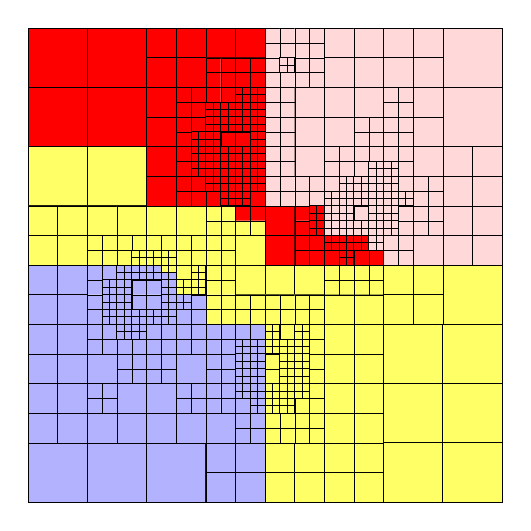
\begin{tikzpicture} [scale=4.3] {
  \begin{scope}[xshift=0cm,yshift=0cm,line width=0.5pt] {
  %\draw [black, opacity=0] (-1.1,-1.1) rectangle (1.1,1.1);  
  \definecolor{lineclr}{RGB}{0,0,0};
  %\definecolor{utorange!30}{RGB}{0,0,255};
  % \definecolor{utsecblue!60}{RGB}{255,255,0};
  % \definecolor{utsecgreen}{RGB}{255,0,0};
  % \definecolor{red!15}{RGB}{0,255,255};
  %\definecolor{fillclr5}{RGB}{0,255,0};
  %\definecolor{fillclr6}{RGB}{255,0,255};
  %\definecolor{fillclr7}{RGB}{255,255,255};
  %\definecolor{fillclr8}{RGB}{0,0,0};
\draw[lineclr, line width=3*0.1pt, fill=utorange!30, opacity=1.0] (-0.700000,-0.700000) -- (-0.525000,-0.700000) -- (-0.525000,-0.525000) -- (-0.700000,-0.525000) -- (-0.700000,-0.700000); 
\draw[lineclr, line width=3*0.1pt, fill=utorange!30, opacity=1.0] (-0.525000,-0.700000) -- (-0.350000,-0.700000) -- (-0.350000,-0.525000) -- (-0.525000,-0.525000) -- (-0.525000,-0.700000); 
\draw[lineclr, line width=3*0.1pt, fill=utorange!30, opacity=1.0] (-0.350000,-0.700000) -- (-0.175000,-0.700000) -- (-0.175000,-0.525000) -- (-0.350000,-0.525000) -- (-0.350000,-0.700000); 
\draw[lineclr, line width=3*0.1pt, fill=utsecblue!60, opacity=1.0] (0.350000,-0.700000) -- (0.525000,-0.700000) -- (0.525000,-0.525000) -- (0.350000,-0.525000) -- (0.350000,-0.700000); 
\draw[lineclr, line width=3*0.1pt, fill=utsecblue!60, opacity=1.0] (0.525000,-0.700000) -- (0.700000,-0.700000) -- (0.700000,-0.525000) -- (0.525000,-0.525000) -- (0.525000,-0.700000); 
\draw[lineclr, line width=3*0.1pt, fill=utsecblue!60, opacity=1.0] (0.350000,-0.525000) -- (0.525000,-0.525000) -- (0.525000,-0.350000) -- (0.350000,-0.350000) -- (0.350000,-0.525000); 
\draw[lineclr, line width=3*0.1pt, fill=utsecblue!60, opacity=1.0] (0.525000,-0.525000) -- (0.700000,-0.525000) -- (0.700000,-0.350000) -- (0.525000,-0.350000) -- (0.525000,-0.525000); 
\draw[lineclr, line width=3*0.1pt, fill=utsecblue!60, opacity=1.0] (0.350000,-0.350000) -- (0.525000,-0.350000) -- (0.525000,-0.175000) -- (0.350000,-0.175000) -- (0.350000,-0.350000); 
\draw[lineclr, line width=3*0.1pt, fill=utsecblue!60, opacity=1.0] (0.525000,-0.350000) -- (0.700000,-0.350000) -- (0.700000,-0.175000) -- (0.525000,-0.175000) -- (0.525000,-0.350000); 
\draw[lineclr, line width=3*0.1pt, fill=utsecblue!60, opacity=1.0] (0.525000,-0.175000) -- (0.700000,-0.175000) -- (0.700000,0.000000) -- (0.525000,0.000000) -- (0.525000,-0.175000); 
\draw[lineclr, line width=3*0.1pt, fill=utsecblue!60, opacity=1.0] (-0.700000,0.175000) -- (-0.525000,0.175000) -- (-0.525000,0.350000) -- (-0.700000,0.350000) -- (-0.700000,0.175000); 
\draw[lineclr, line width=3*0.1pt, fill=utsecblue!60, opacity=1.0] (-0.525000,0.175000) -- (-0.350000,0.175000) -- (-0.350000,0.350000) -- (-0.525000,0.350000) -- (-0.525000,0.175000); 
\draw[lineclr, line width=3*0.1pt, fill=utsecgreen, opacity=1.0] (-0.700000,0.350000) -- (-0.525000,0.350000) -- (-0.525000,0.525000) -- (-0.700000,0.525000) -- (-0.700000,0.350000); 
\draw[lineclr, line width=3*0.1pt, fill=utsecgreen, opacity=1.0] (-0.525000,0.350000) -- (-0.350000,0.350000) -- (-0.350000,0.525000) -- (-0.525000,0.525000) -- (-0.525000,0.350000); 
\draw[lineclr, line width=3*0.1pt, fill=red!15, opacity=1.0] (0.525000,0.350000) -- (0.700000,0.350000) -- (0.700000,0.525000) -- (0.525000,0.525000) -- (0.525000,0.350000); 
\draw[lineclr, line width=3*0.1pt, fill=utsecgreen, opacity=1.0] (-0.700000,0.525000) -- (-0.525000,0.525000) -- (-0.525000,0.700000) -- (-0.700000,0.700000) -- (-0.700000,0.525000); 
\draw[lineclr, line width=3*0.1pt, fill=utsecgreen, opacity=1.0] (-0.525000,0.525000) -- (-0.350000,0.525000) -- (-0.350000,0.700000) -- (-0.525000,0.700000) -- (-0.525000,0.525000); 
\draw[lineclr, line width=3*0.1pt, fill=red!15, opacity=1.0] (0.525000,0.525000) -- (0.700000,0.525000) -- (0.700000,0.700000) -- (0.525000,0.700000) -- (0.525000,0.525000); 
\draw[lineclr, line width=2*0.1pt, fill=utorange!30, opacity=1.0] (-0.175000,-0.700000) -- (-0.087500,-0.700000) -- (-0.087500,-0.612500) -- (-0.175000,-0.612500) -- (-0.175000,-0.700000); 
\draw[lineclr, line width=2*0.1pt, fill=utorange!30, opacity=1.0] (-0.087500,-0.700000) -- (0.000000,-0.700000) -- (0.000000,-0.612500) -- (-0.087500,-0.612500) -- (-0.087500,-0.700000); 
\draw[lineclr, line width=2*0.1pt, fill=utsecblue!60, opacity=1.0] (0.000000,-0.700000) -- (0.087500,-0.700000) -- (0.087500,-0.612500) -- (0.000000,-0.612500) -- (0.000000,-0.700000); 
\draw[lineclr, line width=2*0.1pt, fill=utsecblue!60, opacity=1.0] (0.087500,-0.700000) -- (0.175000,-0.700000) -- (0.175000,-0.612500) -- (0.087500,-0.612500) -- (0.087500,-0.700000); 
\draw[lineclr, line width=2*0.1pt, fill=utsecblue!60, opacity=1.0] (0.175000,-0.700000) -- (0.262500,-0.700000) -- (0.262500,-0.612500) -- (0.175000,-0.612500) -- (0.175000,-0.700000); 
\draw[lineclr, line width=2*0.1pt, fill=utsecblue!60, opacity=1.0] (0.262500,-0.700000) -- (0.350000,-0.700000) -- (0.350000,-0.612500) -- (0.262500,-0.612500) -- (0.262500,-0.700000); 
\draw[lineclr, line width=2*0.1pt, fill=utorange!30, opacity=1.0] (-0.175000,-0.612500) -- (-0.087500,-0.612500) -- (-0.087500,-0.525000) -- (-0.175000,-0.525000) -- (-0.175000,-0.612500); 
\draw[lineclr, line width=2*0.1pt, fill=utorange!30, opacity=1.0] (-0.087500,-0.612500) -- (0.000000,-0.612500) -- (0.000000,-0.525000) -- (-0.087500,-0.525000) -- (-0.087500,-0.612500); 
\draw[lineclr, line width=2*0.1pt, fill=utsecblue!60, opacity=1.0] (0.000000,-0.612500) -- (0.087500,-0.612500) -- (0.087500,-0.525000) -- (0.000000,-0.525000) -- (0.000000,-0.612500); 
\draw[lineclr, line width=2*0.1pt, fill=utsecblue!60, opacity=1.0] (0.087500,-0.612500) -- (0.175000,-0.612500) -- (0.175000,-0.525000) -- (0.087500,-0.525000) -- (0.087500,-0.612500); 
\draw[lineclr, line width=2*0.1pt, fill=utsecblue!60, opacity=1.0] (0.175000,-0.612500) -- (0.262500,-0.612500) -- (0.262500,-0.525000) -- (0.175000,-0.525000) -- (0.175000,-0.612500); 
\draw[lineclr, line width=2*0.1pt, fill=utsecblue!60, opacity=1.0] (0.262500,-0.612500) -- (0.350000,-0.612500) -- (0.350000,-0.525000) -- (0.262500,-0.525000) -- (0.262500,-0.612500); 
\draw[lineclr, line width=2*0.1pt, fill=utorange!30, opacity=1.0] (-0.700000,-0.525000) -- (-0.612500,-0.525000) -- (-0.612500,-0.437500) -- (-0.700000,-0.437500) -- (-0.700000,-0.525000); 
\draw[lineclr, line width=2*0.1pt, fill=utorange!30, opacity=1.0] (-0.612500,-0.525000) -- (-0.525000,-0.525000) -- (-0.525000,-0.437500) -- (-0.612500,-0.437500) -- (-0.612500,-0.525000); 
\draw[lineclr, line width=2*0.1pt, fill=utorange!30, opacity=1.0] (-0.525000,-0.525000) -- (-0.437500,-0.525000) -- (-0.437500,-0.437500) -- (-0.525000,-0.437500) -- (-0.525000,-0.525000); 
\draw[lineclr, line width=2*0.1pt, fill=utorange!30, opacity=1.0] (-0.437500,-0.525000) -- (-0.350000,-0.525000) -- (-0.350000,-0.437500) -- (-0.437500,-0.437500) -- (-0.437500,-0.525000); 
\draw[lineclr, line width=2*0.1pt, fill=utorange!30, opacity=1.0] (-0.350000,-0.525000) -- (-0.262500,-0.525000) -- (-0.262500,-0.437500) -- (-0.350000,-0.437500) -- (-0.350000,-0.525000); 
\draw[lineclr, line width=2*0.1pt, fill=utorange!30, opacity=1.0] (-0.262500,-0.525000) -- (-0.175000,-0.525000) -- (-0.175000,-0.437500) -- (-0.262500,-0.437500) -- (-0.262500,-0.525000); 
\draw[lineclr, line width=2*0.1pt, fill=utorange!30, opacity=1.0] (-0.175000,-0.525000) -- (-0.087500,-0.525000) -- (-0.087500,-0.437500) -- (-0.175000,-0.437500) -- (-0.175000,-0.525000); 
\draw[lineclr, line width=2*0.1pt, fill=utsecblue!60, opacity=1.0] (0.175000,-0.525000) -- (0.262500,-0.525000) -- (0.262500,-0.437500) -- (0.175000,-0.437500) -- (0.175000,-0.525000); 
\draw[lineclr, line width=2*0.1pt, fill=utsecblue!60, opacity=1.0] (0.262500,-0.525000) -- (0.350000,-0.525000) -- (0.350000,-0.437500) -- (0.262500,-0.437500) -- (0.262500,-0.525000); 
\draw[lineclr, line width=2*0.1pt, fill=utorange!30, opacity=1.0] (-0.700000,-0.437500) -- (-0.612500,-0.437500) -- (-0.612500,-0.350000) -- (-0.700000,-0.350000) -- (-0.700000,-0.437500); 
\draw[lineclr, line width=2*0.1pt, fill=utorange!30, opacity=1.0] (-0.612500,-0.437500) -- (-0.525000,-0.437500) -- (-0.525000,-0.350000) -- (-0.612500,-0.350000) -- (-0.612500,-0.437500); 
\draw[lineclr, line width=2*0.1pt, fill=utorange!30, opacity=1.0] (-0.437500,-0.437500) -- (-0.350000,-0.437500) -- (-0.350000,-0.350000) -- (-0.437500,-0.350000) -- (-0.437500,-0.437500); 
\draw[lineclr, line width=2*0.1pt, fill=utorange!30, opacity=1.0] (-0.350000,-0.437500) -- (-0.262500,-0.437500) -- (-0.262500,-0.350000) -- (-0.350000,-0.350000) -- (-0.350000,-0.437500); 
\draw[lineclr, line width=2*0.1pt, fill=utsecblue!60, opacity=1.0] (0.175000,-0.437500) -- (0.262500,-0.437500) -- (0.262500,-0.350000) -- (0.175000,-0.350000) -- (0.175000,-0.437500); 
\draw[lineclr, line width=2*0.1pt, fill=utsecblue!60, opacity=1.0] (0.262500,-0.437500) -- (0.350000,-0.437500) -- (0.350000,-0.350000) -- (0.262500,-0.350000) -- (0.262500,-0.437500); 
\draw[lineclr, line width=2*0.1pt, fill=utorange!30, opacity=1.0] (-0.700000,-0.350000) -- (-0.612500,-0.350000) -- (-0.612500,-0.262500) -- (-0.700000,-0.262500) -- (-0.700000,-0.350000); 
\draw[lineclr, line width=2*0.1pt, fill=utorange!30, opacity=1.0] (-0.612500,-0.350000) -- (-0.525000,-0.350000) -- (-0.525000,-0.262500) -- (-0.612500,-0.262500) -- (-0.612500,-0.350000); 
\draw[lineclr, line width=2*0.1pt, fill=utorange!30, opacity=1.0] (-0.525000,-0.350000) -- (-0.437500,-0.350000) -- (-0.437500,-0.262500) -- (-0.525000,-0.262500) -- (-0.525000,-0.350000); 
\draw[lineclr, line width=2*0.1pt, fill=utorange!30, opacity=1.0] (-0.262500,-0.350000) -- (-0.175000,-0.350000) -- (-0.175000,-0.262500) -- (-0.262500,-0.262500) -- (-0.262500,-0.350000); 
\draw[lineclr, line width=2*0.1pt, fill=utsecblue!60, opacity=1.0] (0.175000,-0.350000) -- (0.262500,-0.350000) -- (0.262500,-0.262500) -- (0.175000,-0.262500) -- (0.175000,-0.350000); 
\draw[lineclr, line width=2*0.1pt, fill=utsecblue!60, opacity=1.0] (0.262500,-0.350000) -- (0.350000,-0.350000) -- (0.350000,-0.262500) -- (0.262500,-0.262500) -- (0.262500,-0.350000); 
\draw[lineclr, line width=2*0.1pt, fill=utorange!30, opacity=1.0] (-0.700000,-0.262500) -- (-0.612500,-0.262500) -- (-0.612500,-0.175000) -- (-0.700000,-0.175000) -- (-0.700000,-0.262500); 
\draw[lineclr, line width=2*0.1pt, fill=utorange!30, opacity=1.0] (-0.612500,-0.262500) -- (-0.525000,-0.262500) -- (-0.525000,-0.175000) -- (-0.612500,-0.175000) -- (-0.612500,-0.262500); 
\draw[lineclr, line width=2*0.1pt, fill=utsecblue!60, opacity=1.0] (0.175000,-0.262500) -- (0.262500,-0.262500) -- (0.262500,-0.175000) -- (0.175000,-0.175000) -- (0.175000,-0.262500); 
\draw[lineclr, line width=2*0.1pt, fill=utsecblue!60, opacity=1.0] (0.262500,-0.262500) -- (0.350000,-0.262500) -- (0.350000,-0.175000) -- (0.262500,-0.175000) -- (0.262500,-0.262500); 
\draw[lineclr, line width=2*0.1pt, fill=utorange!30, opacity=1.0] (-0.700000,-0.175000) -- (-0.612500,-0.175000) -- (-0.612500,-0.087500) -- (-0.700000,-0.087500) -- (-0.700000,-0.175000); 
\draw[lineclr, line width=2*0.1pt, fill=utorange!30, opacity=1.0] (-0.612500,-0.175000) -- (-0.525000,-0.175000) -- (-0.525000,-0.087500) -- (-0.612500,-0.087500) -- (-0.612500,-0.175000); 
\draw[lineclr, line width=2*0.1pt, fill=utsecblue!60, opacity=1.0] (0.175000,-0.175000) -- (0.262500,-0.175000) -- (0.262500,-0.087500) -- (0.175000,-0.087500) -- (0.175000,-0.175000); 
\draw[lineclr, line width=2*0.1pt, fill=utsecblue!60, opacity=1.0] (0.262500,-0.175000) -- (0.350000,-0.175000) -- (0.350000,-0.087500) -- (0.262500,-0.087500) -- (0.262500,-0.175000); 
\draw[lineclr, line width=2*0.1pt, fill=utsecblue!60, opacity=1.0] (0.350000,-0.175000) -- (0.437500,-0.175000) -- (0.437500,-0.087500) -- (0.350000,-0.087500) -- (0.350000,-0.175000); 
\draw[lineclr, line width=2*0.1pt, fill=utsecblue!60, opacity=1.0] (0.437500,-0.175000) -- (0.525000,-0.175000) -- (0.525000,-0.087500) -- (0.437500,-0.087500) -- (0.437500,-0.175000); 
\draw[lineclr, line width=2*0.1pt, fill=utorange!30, opacity=1.0] (-0.700000,-0.087500) -- (-0.612500,-0.087500) -- (-0.612500,0.000000) -- (-0.700000,0.000000) -- (-0.700000,-0.087500); 
\draw[lineclr, line width=2*0.1pt, fill=utorange!30, opacity=1.0] (-0.612500,-0.087500) -- (-0.525000,-0.087500) -- (-0.525000,0.000000) -- (-0.612500,0.000000) -- (-0.612500,-0.087500); 
\draw[lineclr, line width=2*0.1pt, fill=utsecblue!60, opacity=1.0] (-0.087500,-0.087500) -- (0.000000,-0.087500) -- (0.000000,0.000000) -- (-0.087500,0.000000) -- (-0.087500,-0.087500); 
\draw[lineclr, line width=2*0.1pt, fill=utsecblue!60, opacity=1.0] (0.000000,-0.087500) -- (0.087500,-0.087500) -- (0.087500,0.000000) -- (0.000000,0.000000) -- (0.000000,-0.087500); 
\draw[lineclr, line width=2*0.1pt, fill=utsecblue!60, opacity=1.0] (0.087500,-0.087500) -- (0.175000,-0.087500) -- (0.175000,0.000000) -- (0.087500,0.000000) -- (0.087500,-0.087500); 
\draw[lineclr, line width=2*0.1pt, fill=utsecblue!60, opacity=1.0] (0.350000,-0.087500) -- (0.437500,-0.087500) -- (0.437500,0.000000) -- (0.350000,0.000000) -- (0.350000,-0.087500); 
\draw[lineclr, line width=2*0.1pt, fill=utsecblue!60, opacity=1.0] (0.437500,-0.087500) -- (0.525000,-0.087500) -- (0.525000,0.000000) -- (0.437500,0.000000) -- (0.437500,-0.087500); 
\draw[lineclr, line width=2*0.1pt, fill=utsecblue!60, opacity=1.0] (-0.700000,0.000000) -- (-0.612500,0.000000) -- (-0.612500,0.087500) -- (-0.700000,0.087500) -- (-0.700000,0.000000); 
\draw[lineclr, line width=2*0.1pt, fill=utsecblue!60, opacity=1.0] (-0.612500,0.000000) -- (-0.525000,0.000000) -- (-0.525000,0.087500) -- (-0.612500,0.087500) -- (-0.612500,0.000000); 
\draw[lineclr, line width=2*0.1pt, fill=utsecblue!60, opacity=1.0] (-0.087500,0.000000) -- (0.000000,0.000000) -- (0.000000,0.087500) -- (-0.087500,0.087500) -- (-0.087500,0.000000); 
\draw[lineclr, line width=2*0.1pt, fill=utsecgreen, opacity=1.0] (0.000000,0.000000) -- (0.087500,0.000000) -- (0.087500,0.087500) -- (0.000000,0.087500) -- (0.000000,0.000000); 
\draw[lineclr, line width=2*0.1pt, fill=red!15, opacity=1.0] (0.437500,0.000000) -- (0.525000,0.000000) -- (0.525000,0.087500) -- (0.437500,0.087500) -- (0.437500,0.000000); 
\draw[lineclr, line width=2*0.1pt, fill=red!15, opacity=1.0] (0.525000,0.000000) -- (0.612500,0.000000) -- (0.612500,0.087500) -- (0.525000,0.087500) -- (0.525000,0.000000); 
\draw[lineclr, line width=2*0.1pt, fill=red!15, opacity=1.0] (0.612500,0.000000) -- (0.700000,0.000000) -- (0.700000,0.087500) -- (0.612500,0.087500) -- (0.612500,0.000000); 
\draw[lineclr, line width=2*0.1pt, fill=utsecblue!60, opacity=1.0] (-0.700000,0.087500) -- (-0.612500,0.087500) -- (-0.612500,0.175000) -- (-0.700000,0.175000) -- (-0.700000,0.087500); 
\draw[lineclr, line width=2*0.1pt, fill=utsecblue!60, opacity=1.0] (-0.612500,0.087500) -- (-0.525000,0.087500) -- (-0.525000,0.175000) -- (-0.612500,0.175000) -- (-0.612500,0.087500); 
\draw[lineclr, line width=2*0.1pt, fill=utsecblue!60, opacity=1.0] (-0.525000,0.087500) -- (-0.437500,0.087500) -- (-0.437500,0.175000) -- (-0.525000,0.175000) -- (-0.525000,0.087500); 
\draw[lineclr, line width=2*0.1pt, fill=utsecblue!60, opacity=1.0] (-0.437500,0.087500) -- (-0.350000,0.087500) -- (-0.350000,0.175000) -- (-0.437500,0.175000) -- (-0.437500,0.087500); 
\draw[lineclr, line width=2*0.1pt, fill=utsecblue!60, opacity=1.0] (-0.350000,0.087500) -- (-0.262500,0.087500) -- (-0.262500,0.175000) -- (-0.350000,0.175000) -- (-0.350000,0.087500); 
\draw[lineclr, line width=2*0.1pt, fill=utsecblue!60, opacity=1.0] (-0.262500,0.087500) -- (-0.175000,0.087500) -- (-0.175000,0.175000) -- (-0.262500,0.175000) -- (-0.262500,0.087500); 
\draw[lineclr, line width=2*0.1pt, fill=utsecgreen, opacity=1.0] (0.000000,0.087500) -- (0.087500,0.087500) -- (0.087500,0.175000) -- (0.000000,0.175000) -- (0.000000,0.087500); 
\draw[lineclr, line width=2*0.1pt, fill=red!15, opacity=1.0] (0.525000,0.087500) -- (0.612500,0.087500) -- (0.612500,0.175000) -- (0.525000,0.175000) -- (0.525000,0.087500); 
\draw[lineclr, line width=2*0.1pt, fill=red!15, opacity=1.0] (0.612500,0.087500) -- (0.700000,0.087500) -- (0.700000,0.175000) -- (0.612500,0.175000) -- (0.612500,0.087500); 
\draw[lineclr, line width=2*0.1pt, fill=utsecgreen, opacity=1.0] (-0.350000,0.175000) -- (-0.262500,0.175000) -- (-0.262500,0.262500) -- (-0.350000,0.262500) -- (-0.350000,0.175000); 
\draw[lineclr, line width=2*0.1pt, fill=red!15, opacity=1.0] (0.525000,0.175000) -- (0.612500,0.175000) -- (0.612500,0.262500) -- (0.525000,0.262500) -- (0.525000,0.175000); 
\draw[lineclr, line width=2*0.1pt, fill=red!15, opacity=1.0] (0.612500,0.175000) -- (0.700000,0.175000) -- (0.700000,0.262500) -- (0.612500,0.262500) -- (0.612500,0.175000); 
\draw[lineclr, line width=2*0.1pt, fill=utsecgreen, opacity=1.0] (-0.350000,0.262500) -- (-0.262500,0.262500) -- (-0.262500,0.350000) -- (-0.350000,0.350000) -- (-0.350000,0.262500); 
\draw[lineclr, line width=2*0.1pt, fill=red!15, opacity=1.0] (0.087500,0.262500) -- (0.175000,0.262500) -- (0.175000,0.350000) -- (0.087500,0.350000) -- (0.087500,0.262500); 
\draw[lineclr, line width=2*0.1pt, fill=red!15, opacity=1.0] (0.437500,0.262500) -- (0.525000,0.262500) -- (0.525000,0.350000) -- (0.437500,0.350000) -- (0.437500,0.262500); 
\draw[lineclr, line width=2*0.1pt, fill=red!15, opacity=1.0] (0.525000,0.262500) -- (0.612500,0.262500) -- (0.612500,0.350000) -- (0.525000,0.350000) -- (0.525000,0.262500); 
\draw[lineclr, line width=2*0.1pt, fill=red!15, opacity=1.0] (0.612500,0.262500) -- (0.700000,0.262500) -- (0.700000,0.350000) -- (0.612500,0.350000) -- (0.612500,0.262500); 
\draw[lineclr, line width=2*0.1pt, fill=utsecgreen, opacity=1.0] (-0.350000,0.350000) -- (-0.262500,0.350000) -- (-0.262500,0.437500) -- (-0.350000,0.437500) -- (-0.350000,0.350000); 
\draw[lineclr, line width=2*0.1pt, fill=red!15, opacity=1.0] (0.087500,0.350000) -- (0.175000,0.350000) -- (0.175000,0.437500) -- (0.087500,0.437500) -- (0.087500,0.350000); 
\draw[lineclr, line width=2*0.1pt, fill=red!15, opacity=1.0] (0.175000,0.350000) -- (0.262500,0.350000) -- (0.262500,0.437500) -- (0.175000,0.437500) -- (0.175000,0.350000); 
\draw[lineclr, line width=2*0.1pt, fill=red!15, opacity=1.0] (0.437500,0.350000) -- (0.525000,0.350000) -- (0.525000,0.437500) -- (0.437500,0.437500) -- (0.437500,0.350000); 
\draw[lineclr, line width=2*0.1pt, fill=utsecgreen, opacity=1.0] (-0.350000,0.437500) -- (-0.262500,0.437500) -- (-0.262500,0.525000) -- (-0.350000,0.525000) -- (-0.350000,0.437500); 
\draw[lineclr, line width=2*0.1pt, fill=red!15, opacity=1.0] (0.087500,0.437500) -- (0.175000,0.437500) -- (0.175000,0.525000) -- (0.087500,0.525000) -- (0.087500,0.437500); 
\draw[lineclr, line width=2*0.1pt, fill=red!15, opacity=1.0] (0.175000,0.437500) -- (0.262500,0.437500) -- (0.262500,0.525000) -- (0.175000,0.525000) -- (0.175000,0.437500); 
\draw[lineclr, line width=2*0.1pt, fill=red!15, opacity=1.0] (0.262500,0.437500) -- (0.350000,0.437500) -- (0.350000,0.525000) -- (0.262500,0.525000) -- (0.262500,0.437500); 
\draw[lineclr, line width=2*0.1pt, fill=red!15, opacity=1.0] (0.437500,0.437500) -- (0.525000,0.437500) -- (0.525000,0.525000) -- (0.437500,0.525000) -- (0.437500,0.437500); 
\draw[lineclr, line width=2*0.1pt, fill=utsecgreen, opacity=1.0] (-0.350000,0.525000) -- (-0.262500,0.525000) -- (-0.262500,0.612500) -- (-0.350000,0.612500) -- (-0.350000,0.525000); 
\draw[lineclr, line width=2*0.1pt, fill=utsecgreen, opacity=1.0] (-0.262500,0.525000) -- (-0.175000,0.525000) -- (-0.175000,0.612500) -- (-0.262500,0.612500) -- (-0.262500,0.525000); 
\draw[lineclr, line width=2*0.1pt, fill=red!15, opacity=1.0] (0.175000,0.525000) -- (0.262500,0.525000) -- (0.262500,0.612500) -- (0.175000,0.612500) -- (0.175000,0.525000); 
\draw[lineclr, line width=2*0.1pt, fill=red!15, opacity=1.0] (0.262500,0.525000) -- (0.350000,0.525000) -- (0.350000,0.612500) -- (0.262500,0.612500) -- (0.262500,0.525000); 
\draw[lineclr, line width=2*0.1pt, fill=red!15, opacity=1.0] (0.350000,0.525000) -- (0.437500,0.525000) -- (0.437500,0.612500) -- (0.350000,0.612500) -- (0.350000,0.525000); 
\draw[lineclr, line width=2*0.1pt, fill=red!15, opacity=1.0] (0.437500,0.525000) -- (0.525000,0.525000) -- (0.525000,0.612500) -- (0.437500,0.612500) -- (0.437500,0.525000); 
\draw[lineclr, line width=2*0.1pt, fill=utsecgreen, opacity=1.0] (-0.350000,0.612500) -- (-0.262500,0.612500) -- (-0.262500,0.700000) -- (-0.350000,0.700000) -- (-0.350000,0.612500); 
\draw[lineclr, line width=2*0.1pt, fill=utsecgreen, opacity=1.0] (-0.262500,0.612500) -- (-0.175000,0.612500) -- (-0.175000,0.700000) -- (-0.262500,0.700000) -- (-0.262500,0.612500); 
\draw[lineclr, line width=2*0.1pt, fill=utsecgreen, opacity=1.0] (-0.175000,0.612500) -- (-0.087500,0.612500) -- (-0.087500,0.700000) -- (-0.175000,0.700000) -- (-0.175000,0.612500); 
\draw[lineclr, line width=2*0.1pt, fill=utsecgreen, opacity=1.0] (-0.087500,0.612500) -- (0.000000,0.612500) -- (0.000000,0.700000) -- (-0.087500,0.700000) -- (-0.087500,0.612500); 
\draw[lineclr, line width=2*0.1pt, fill=red!15, opacity=1.0] (0.175000,0.612500) -- (0.262500,0.612500) -- (0.262500,0.700000) -- (0.175000,0.700000) -- (0.175000,0.612500); 
\draw[lineclr, line width=2*0.1pt, fill=red!15, opacity=1.0] (0.262500,0.612500) -- (0.350000,0.612500) -- (0.350000,0.700000) -- (0.262500,0.700000) -- (0.262500,0.612500); 
\draw[lineclr, line width=2*0.1pt, fill=red!15, opacity=1.0] (0.350000,0.612500) -- (0.437500,0.612500) -- (0.437500,0.700000) -- (0.350000,0.700000) -- (0.350000,0.612500); 
\draw[lineclr, line width=2*0.1pt, fill=red!15, opacity=1.0] (0.437500,0.612500) -- (0.525000,0.612500) -- (0.525000,0.700000) -- (0.437500,0.700000) -- (0.437500,0.612500); 
\draw[lineclr, line width=1*0.1pt, fill=utorange!30, opacity=1.0] (-0.087500,-0.525000) -- (-0.043750,-0.525000) -- (-0.043750,-0.481250) -- (-0.087500,-0.481250) -- (-0.087500,-0.525000); 
\draw[lineclr, line width=1*0.1pt, fill=utorange!30, opacity=1.0] (-0.043750,-0.525000) -- (0.000000,-0.525000) -- (0.000000,-0.481250) -- (-0.043750,-0.481250) -- (-0.043750,-0.525000); 
\draw[lineclr, line width=1*0.1pt, fill=utsecblue!60, opacity=1.0] (0.000000,-0.525000) -- (0.043750,-0.525000) -- (0.043750,-0.481250) -- (0.000000,-0.481250) -- (0.000000,-0.525000); 
\draw[lineclr, line width=1*0.1pt, fill=utsecblue!60, opacity=1.0] (0.043750,-0.525000) -- (0.087500,-0.525000) -- (0.087500,-0.481250) -- (0.043750,-0.481250) -- (0.043750,-0.525000); 
\draw[lineclr, line width=1*0.1pt, fill=utsecblue!60, opacity=1.0] (0.087500,-0.525000) -- (0.131250,-0.525000) -- (0.131250,-0.481250) -- (0.087500,-0.481250) -- (0.087500,-0.525000); 
\draw[lineclr, line width=1*0.1pt, fill=utsecblue!60, opacity=1.0] (0.131250,-0.525000) -- (0.175000,-0.525000) -- (0.175000,-0.481250) -- (0.131250,-0.481250) -- (0.131250,-0.525000); 
\draw[lineclr, line width=1*0.1pt, fill=utorange!30, opacity=1.0] (-0.087500,-0.481250) -- (-0.043750,-0.481250) -- (-0.043750,-0.437500) -- (-0.087500,-0.437500) -- (-0.087500,-0.481250); 
\draw[lineclr, line width=1*0.1pt, fill=utorange!30, opacity=1.0] (-0.043750,-0.481250) -- (0.000000,-0.481250) -- (0.000000,-0.437500) -- (-0.043750,-0.437500) -- (-0.043750,-0.481250); 
\draw[lineclr, line width=1*0.1pt, fill=utsecblue!60, opacity=1.0] (0.000000,-0.481250) -- (0.043750,-0.481250) -- (0.043750,-0.437500) -- (0.000000,-0.437500) -- (0.000000,-0.481250); 
\draw[lineclr, line width=1*0.1pt, fill=utsecblue!60, opacity=1.0] (0.043750,-0.481250) -- (0.087500,-0.481250) -- (0.087500,-0.437500) -- (0.043750,-0.437500) -- (0.043750,-0.481250); 
\draw[lineclr, line width=1*0.1pt, fill=utsecblue!60, opacity=1.0] (0.087500,-0.481250) -- (0.131250,-0.481250) -- (0.131250,-0.437500) -- (0.087500,-0.437500) -- (0.087500,-0.481250); 
\draw[lineclr, line width=1*0.1pt, fill=utsecblue!60, opacity=1.0] (0.131250,-0.481250) -- (0.175000,-0.481250) -- (0.175000,-0.437500) -- (0.131250,-0.437500) -- (0.131250,-0.481250); 
\draw[lineclr, line width=1*0.1pt, fill=utorange!30, opacity=1.0] (-0.525000,-0.437500) -- (-0.481250,-0.437500) -- (-0.481250,-0.393750) -- (-0.525000,-0.393750) -- (-0.525000,-0.437500); 
\draw[lineclr, line width=1*0.1pt, fill=utorange!30, opacity=1.0] (-0.481250,-0.437500) -- (-0.437500,-0.437500) -- (-0.437500,-0.393750) -- (-0.481250,-0.393750) -- (-0.481250,-0.437500); 
\draw[lineclr, line width=1*0.1pt, fill=utorange!30, opacity=1.0] (-0.262500,-0.437500) -- (-0.218750,-0.437500) -- (-0.218750,-0.393750) -- (-0.262500,-0.393750) -- (-0.262500,-0.437500); 
\draw[lineclr, line width=1*0.1pt, fill=utorange!30, opacity=1.0] (-0.218750,-0.437500) -- (-0.175000,-0.437500) -- (-0.175000,-0.393750) -- (-0.218750,-0.393750) -- (-0.218750,-0.437500); 
\draw[lineclr, line width=1*0.1pt, fill=utorange!30, opacity=1.0] (-0.175000,-0.437500) -- (-0.131250,-0.437500) -- (-0.131250,-0.393750) -- (-0.175000,-0.393750) -- (-0.175000,-0.437500); 
\draw[lineclr, line width=1*0.1pt, fill=utorange!30, opacity=1.0] (-0.131250,-0.437500) -- (-0.087500,-0.437500) -- (-0.087500,-0.393750) -- (-0.131250,-0.393750) -- (-0.131250,-0.437500); 
\draw[lineclr, line width=1*0.1pt, fill=utorange!30, opacity=1.0] (-0.087500,-0.437500) -- (-0.043750,-0.437500) -- (-0.043750,-0.393750) -- (-0.087500,-0.393750) -- (-0.087500,-0.437500); 
\draw[lineclr, line width=1*0.1pt, fill=utsecblue!60, opacity=1.0] (0.087500,-0.437500) -- (0.131250,-0.437500) -- (0.131250,-0.393750) -- (0.087500,-0.393750) -- (0.087500,-0.437500); 
\draw[lineclr, line width=1*0.1pt, fill=utsecblue!60, opacity=1.0] (0.131250,-0.437500) -- (0.175000,-0.437500) -- (0.175000,-0.393750) -- (0.131250,-0.393750) -- (0.131250,-0.437500); 
\draw[lineclr, line width=1*0.1pt, fill=utorange!30, opacity=1.0] (-0.525000,-0.393750) -- (-0.481250,-0.393750) -- (-0.481250,-0.350000) -- (-0.525000,-0.350000) -- (-0.525000,-0.393750); 
\draw[lineclr, line width=1*0.1pt, fill=utorange!30, opacity=1.0] (-0.481250,-0.393750) -- (-0.437500,-0.393750) -- (-0.437500,-0.350000) -- (-0.481250,-0.350000) -- (-0.481250,-0.393750); 
\draw[lineclr, line width=1*0.1pt, fill=utorange!30, opacity=1.0] (-0.262500,-0.393750) -- (-0.218750,-0.393750) -- (-0.218750,-0.350000) -- (-0.262500,-0.350000) -- (-0.262500,-0.393750); 
\draw[lineclr, line width=1*0.1pt, fill=utorange!30, opacity=1.0] (-0.218750,-0.393750) -- (-0.175000,-0.393750) -- (-0.175000,-0.350000) -- (-0.218750,-0.350000) -- (-0.218750,-0.393750); 
\draw[lineclr, line width=1*0.1pt, fill=utorange!30, opacity=1.0] (-0.175000,-0.393750) -- (-0.131250,-0.393750) -- (-0.131250,-0.350000) -- (-0.175000,-0.350000) -- (-0.175000,-0.393750); 
\draw[lineclr, line width=1*0.1pt, fill=utorange!30, opacity=1.0] (-0.131250,-0.393750) -- (-0.087500,-0.393750) -- (-0.087500,-0.350000) -- (-0.131250,-0.350000) -- (-0.131250,-0.393750); 
\draw[lineclr, line width=1*0.1pt, fill=utsecblue!60, opacity=1.0] (0.131250,-0.393750) -- (0.175000,-0.393750) -- (0.175000,-0.350000) -- (0.131250,-0.350000) -- (0.131250,-0.393750); 
\draw[lineclr, line width=1*0.1pt, fill=utorange!30, opacity=1.0] (-0.437500,-0.350000) -- (-0.393750,-0.350000) -- (-0.393750,-0.306250) -- (-0.437500,-0.306250) -- (-0.437500,-0.350000); 
\draw[lineclr, line width=1*0.1pt, fill=utorange!30, opacity=1.0] (-0.393750,-0.350000) -- (-0.350000,-0.350000) -- (-0.350000,-0.306250) -- (-0.393750,-0.306250) -- (-0.393750,-0.350000); 
\draw[lineclr, line width=1*0.1pt, fill=utorange!30, opacity=1.0] (-0.350000,-0.350000) -- (-0.306250,-0.350000) -- (-0.306250,-0.306250) -- (-0.350000,-0.306250) -- (-0.350000,-0.350000); 
\draw[lineclr, line width=1*0.1pt, fill=utorange!30, opacity=1.0] (-0.306250,-0.350000) -- (-0.262500,-0.350000) -- (-0.262500,-0.306250) -- (-0.306250,-0.306250) -- (-0.306250,-0.350000); 
\draw[lineclr, line width=1*0.1pt, fill=utorange!30, opacity=1.0] (-0.175000,-0.350000) -- (-0.131250,-0.350000) -- (-0.131250,-0.306250) -- (-0.175000,-0.306250) -- (-0.175000,-0.350000); 
\draw[lineclr, line width=1*0.1pt, fill=utorange!30, opacity=1.0] (-0.131250,-0.350000) -- (-0.087500,-0.350000) -- (-0.087500,-0.306250) -- (-0.131250,-0.306250) -- (-0.131250,-0.350000); 
\draw[lineclr, line width=1*0.1pt, fill=utsecblue!60, opacity=1.0] (0.000000,-0.350000) -- (0.043750,-0.350000) -- (0.043750,-0.306250) -- (0.000000,-0.306250) -- (0.000000,-0.350000); 
\draw[lineclr, line width=1*0.1pt, fill=utsecblue!60, opacity=1.0] (0.131250,-0.350000) -- (0.175000,-0.350000) -- (0.175000,-0.306250) -- (0.131250,-0.306250) -- (0.131250,-0.350000); 
\draw[lineclr, line width=1*0.1pt, fill=utorange!30, opacity=1.0] (-0.437500,-0.306250) -- (-0.393750,-0.306250) -- (-0.393750,-0.262500) -- (-0.437500,-0.262500) -- (-0.437500,-0.306250); 
\draw[lineclr, line width=1*0.1pt, fill=utorange!30, opacity=1.0] (-0.393750,-0.306250) -- (-0.350000,-0.306250) -- (-0.350000,-0.262500) -- (-0.393750,-0.262500) -- (-0.393750,-0.306250); 
\draw[lineclr, line width=1*0.1pt, fill=utorange!30, opacity=1.0] (-0.350000,-0.306250) -- (-0.306250,-0.306250) -- (-0.306250,-0.262500) -- (-0.350000,-0.262500) -- (-0.350000,-0.306250); 
\draw[lineclr, line width=1*0.1pt, fill=utorange!30, opacity=1.0] (-0.306250,-0.306250) -- (-0.262500,-0.306250) -- (-0.262500,-0.262500) -- (-0.306250,-0.262500) -- (-0.306250,-0.306250); 
\draw[lineclr, line width=1*0.1pt, fill=utorange!30, opacity=1.0] (-0.175000,-0.306250) -- (-0.131250,-0.306250) -- (-0.131250,-0.262500) -- (-0.175000,-0.262500) -- (-0.175000,-0.306250); 
\draw[lineclr, line width=1*0.1pt, fill=utorange!30, opacity=1.0] (-0.131250,-0.306250) -- (-0.087500,-0.306250) -- (-0.087500,-0.262500) -- (-0.131250,-0.262500) -- (-0.131250,-0.306250); 
\draw[lineclr, line width=1*0.1pt, fill=utsecblue!60, opacity=1.0] (0.000000,-0.306250) -- (0.043750,-0.306250) -- (0.043750,-0.262500) -- (0.000000,-0.262500) -- (0.000000,-0.306250); 
\draw[lineclr, line width=1*0.1pt, fill=utsecblue!60, opacity=1.0] (0.131250,-0.306250) -- (0.175000,-0.306250) -- (0.175000,-0.262500) -- (0.131250,-0.262500) -- (0.131250,-0.306250); 
\draw[lineclr, line width=1*0.1pt, fill=utorange!30, opacity=1.0] (-0.525000,-0.262500) -- (-0.481250,-0.262500) -- (-0.481250,-0.218750) -- (-0.525000,-0.218750) -- (-0.525000,-0.262500); 
\draw[lineclr, line width=1*0.1pt, fill=utorange!30, opacity=1.0] (-0.481250,-0.262500) -- (-0.437500,-0.262500) -- (-0.437500,-0.218750) -- (-0.481250,-0.218750) -- (-0.481250,-0.262500); 
\draw[lineclr, line width=1*0.1pt, fill=utorange!30, opacity=1.0] (-0.437500,-0.262500) -- (-0.393750,-0.262500) -- (-0.393750,-0.218750) -- (-0.437500,-0.218750) -- (-0.437500,-0.262500); 
\draw[lineclr, line width=1*0.1pt, fill=utorange!30, opacity=1.0] (-0.393750,-0.262500) -- (-0.350000,-0.262500) -- (-0.350000,-0.218750) -- (-0.393750,-0.218750) -- (-0.393750,-0.262500); 
\draw[lineclr, line width=1*0.1pt, fill=utorange!30, opacity=1.0] (-0.350000,-0.262500) -- (-0.306250,-0.262500) -- (-0.306250,-0.218750) -- (-0.350000,-0.218750) -- (-0.350000,-0.262500); 
\draw[lineclr, line width=1*0.1pt, fill=utorange!30, opacity=1.0] (-0.306250,-0.262500) -- (-0.262500,-0.262500) -- (-0.262500,-0.218750) -- (-0.306250,-0.218750) -- (-0.306250,-0.262500); 
\draw[lineclr, line width=1*0.1pt, fill=utorange!30, opacity=1.0] (-0.262500,-0.262500) -- (-0.218750,-0.262500) -- (-0.218750,-0.218750) -- (-0.262500,-0.218750) -- (-0.262500,-0.262500); 
\draw[lineclr, line width=1*0.1pt, fill=utorange!30, opacity=1.0] (-0.218750,-0.262500) -- (-0.175000,-0.262500) -- (-0.175000,-0.218750) -- (-0.218750,-0.218750) -- (-0.218750,-0.262500); 
\draw[lineclr, line width=1*0.1pt, fill=utorange!30, opacity=1.0] (-0.175000,-0.262500) -- (-0.131250,-0.262500) -- (-0.131250,-0.218750) -- (-0.175000,-0.218750) -- (-0.175000,-0.262500); 
\draw[lineclr, line width=1*0.1pt, fill=utorange!30, opacity=1.0] (-0.131250,-0.262500) -- (-0.087500,-0.262500) -- (-0.087500,-0.218750) -- (-0.131250,-0.218750) -- (-0.131250,-0.262500); 
\draw[lineclr, line width=1*0.1pt, fill=utsecblue!60, opacity=1.0] (0.131250,-0.262500) -- (0.175000,-0.262500) -- (0.175000,-0.218750) -- (0.131250,-0.218750) -- (0.131250,-0.262500); 
\draw[lineclr, line width=1*0.1pt, fill=utorange!30, opacity=1.0] (-0.525000,-0.218750) -- (-0.481250,-0.218750) -- (-0.481250,-0.175000) -- (-0.525000,-0.175000) -- (-0.525000,-0.218750); 
\draw[lineclr, line width=1*0.1pt, fill=utorange!30, opacity=1.0] (-0.481250,-0.218750) -- (-0.437500,-0.218750) -- (-0.437500,-0.175000) -- (-0.481250,-0.175000) -- (-0.481250,-0.218750); 
\draw[lineclr, line width=1*0.1pt, fill=utorange!30, opacity=1.0] (-0.350000,-0.218750) -- (-0.306250,-0.218750) -- (-0.306250,-0.175000) -- (-0.350000,-0.175000) -- (-0.350000,-0.218750); 
\draw[lineclr, line width=1*0.1pt, fill=utorange!30, opacity=1.0] (-0.306250,-0.218750) -- (-0.262500,-0.218750) -- (-0.262500,-0.175000) -- (-0.306250,-0.175000) -- (-0.306250,-0.218750); 
\draw[lineclr, line width=1*0.1pt, fill=utorange!30, opacity=1.0] (-0.262500,-0.218750) -- (-0.218750,-0.218750) -- (-0.218750,-0.175000) -- (-0.262500,-0.175000) -- (-0.262500,-0.218750); 
\draw[lineclr, line width=1*0.1pt, fill=utorange!30, opacity=1.0] (-0.218750,-0.218750) -- (-0.175000,-0.218750) -- (-0.175000,-0.175000) -- (-0.218750,-0.175000) -- (-0.218750,-0.218750); 
\draw[lineclr, line width=1*0.1pt, fill=utorange!30, opacity=1.0] (-0.175000,-0.218750) -- (-0.131250,-0.218750) -- (-0.131250,-0.175000) -- (-0.175000,-0.175000) -- (-0.175000,-0.218750); 
\draw[lineclr, line width=1*0.1pt, fill=utorange!30, opacity=1.0] (-0.131250,-0.218750) -- (-0.087500,-0.218750) -- (-0.087500,-0.175000) -- (-0.131250,-0.175000) -- (-0.131250,-0.218750); 
\draw[lineclr, line width=1*0.1pt, fill=utorange!30, opacity=1.0] (-0.087500,-0.218750) -- (-0.043750,-0.218750) -- (-0.043750,-0.175000) -- (-0.087500,-0.175000) -- (-0.087500,-0.218750); 
\draw[lineclr, line width=1*0.1pt, fill=utorange!30, opacity=1.0] (-0.043750,-0.218750) -- (0.000000,-0.218750) -- (0.000000,-0.175000) -- (-0.043750,-0.175000) -- (-0.043750,-0.218750); 
\draw[lineclr, line width=1*0.1pt, fill=utsecblue!60, opacity=1.0] (0.043750,-0.218750) -- (0.087500,-0.218750) -- (0.087500,-0.175000) -- (0.043750,-0.175000) -- (0.043750,-0.218750); 
\draw[lineclr, line width=1*0.1pt, fill=utsecblue!60, opacity=1.0] (0.131250,-0.218750) -- (0.175000,-0.218750) -- (0.175000,-0.175000) -- (0.131250,-0.175000) -- (0.131250,-0.218750); 
\draw[lineclr, line width=1*0.1pt, fill=utorange!30, opacity=1.0] (-0.525000,-0.175000) -- (-0.481250,-0.175000) -- (-0.481250,-0.131250) -- (-0.525000,-0.131250) -- (-0.525000,-0.175000); 
\draw[lineclr, line width=1*0.1pt, fill=utorange!30, opacity=1.0] (-0.262500,-0.175000) -- (-0.218750,-0.175000) -- (-0.218750,-0.131250) -- (-0.262500,-0.131250) -- (-0.262500,-0.175000); 
\draw[lineclr, line width=1*0.1pt, fill=utorange!30, opacity=1.0] (-0.218750,-0.175000) -- (-0.175000,-0.175000) -- (-0.175000,-0.131250) -- (-0.218750,-0.131250) -- (-0.218750,-0.175000); 
\draw[lineclr, line width=1*0.1pt, fill=utsecblue!60, opacity=1.0] (-0.175000,-0.175000) -- (-0.131250,-0.175000) -- (-0.131250,-0.131250) -- (-0.175000,-0.131250) -- (-0.175000,-0.175000); 
\draw[lineclr, line width=1*0.1pt, fill=utsecblue!60, opacity=1.0] (-0.131250,-0.175000) -- (-0.087500,-0.175000) -- (-0.087500,-0.131250) -- (-0.131250,-0.131250) -- (-0.131250,-0.175000); 
\draw[lineclr, line width=1*0.1pt, fill=utsecblue!60, opacity=1.0] (-0.087500,-0.175000) -- (-0.043750,-0.175000) -- (-0.043750,-0.131250) -- (-0.087500,-0.131250) -- (-0.087500,-0.175000); 
\draw[lineclr, line width=1*0.1pt, fill=utsecblue!60, opacity=1.0] (-0.043750,-0.175000) -- (0.000000,-0.175000) -- (0.000000,-0.131250) -- (-0.043750,-0.131250) -- (-0.043750,-0.175000); 
\draw[lineclr, line width=1*0.1pt, fill=utsecblue!60, opacity=1.0] (0.000000,-0.175000) -- (0.043750,-0.175000) -- (0.043750,-0.131250) -- (0.000000,-0.131250) -- (0.000000,-0.175000); 
\draw[lineclr, line width=1*0.1pt, fill=utsecblue!60, opacity=1.0] (0.043750,-0.175000) -- (0.087500,-0.175000) -- (0.087500,-0.131250) -- (0.043750,-0.131250) -- (0.043750,-0.175000); 
\draw[lineclr, line width=1*0.1pt, fill=utsecblue!60, opacity=1.0] (0.087500,-0.175000) -- (0.131250,-0.175000) -- (0.131250,-0.131250) -- (0.087500,-0.131250) -- (0.087500,-0.175000); 
\draw[lineclr, line width=1*0.1pt, fill=utsecblue!60, opacity=1.0] (0.131250,-0.175000) -- (0.175000,-0.175000) -- (0.175000,-0.131250) -- (0.131250,-0.131250) -- (0.131250,-0.175000); 
\draw[lineclr, line width=1*0.1pt, fill=utorange!30, opacity=1.0] (-0.525000,-0.131250) -- (-0.481250,-0.131250) -- (-0.481250,-0.087500) -- (-0.525000,-0.087500) -- (-0.525000,-0.131250); 
\draw[lineclr, line width=1*0.1pt, fill=utorange!30, opacity=1.0] (-0.393750,-0.131250) -- (-0.350000,-0.131250) -- (-0.350000,-0.087500) -- (-0.393750,-0.087500) -- (-0.393750,-0.131250); 
\draw[lineclr, line width=1*0.1pt, fill=utorange!30, opacity=1.0] (-0.350000,-0.131250) -- (-0.306250,-0.131250) -- (-0.306250,-0.087500) -- (-0.350000,-0.087500) -- (-0.350000,-0.131250); 
\draw[lineclr, line width=1*0.1pt, fill=utorange!30, opacity=1.0] (-0.218750,-0.131250) -- (-0.175000,-0.131250) -- (-0.175000,-0.087500) -- (-0.218750,-0.087500) -- (-0.218750,-0.131250); 
\draw[lineclr, line width=1*0.1pt, fill=utsecblue!60, opacity=1.0] (-0.175000,-0.131250) -- (-0.131250,-0.131250) -- (-0.131250,-0.087500) -- (-0.175000,-0.087500) -- (-0.175000,-0.131250); 
\draw[lineclr, line width=1*0.1pt, fill=utsecblue!60, opacity=1.0] (-0.131250,-0.131250) -- (-0.087500,-0.131250) -- (-0.087500,-0.087500) -- (-0.131250,-0.087500) -- (-0.131250,-0.131250); 
\draw[lineclr, line width=1*0.1pt, fill=utsecblue!60, opacity=1.0] (-0.087500,-0.131250) -- (-0.043750,-0.131250) -- (-0.043750,-0.087500) -- (-0.087500,-0.087500) -- (-0.087500,-0.131250); 
\draw[lineclr, line width=1*0.1pt, fill=utsecblue!60, opacity=1.0] (-0.043750,-0.131250) -- (0.000000,-0.131250) -- (0.000000,-0.087500) -- (-0.043750,-0.087500) -- (-0.043750,-0.131250); 
\draw[lineclr, line width=1*0.1pt, fill=utsecblue!60, opacity=1.0] (0.000000,-0.131250) -- (0.043750,-0.131250) -- (0.043750,-0.087500) -- (0.000000,-0.087500) -- (0.000000,-0.131250); 
\draw[lineclr, line width=1*0.1pt, fill=utsecblue!60, opacity=1.0] (0.043750,-0.131250) -- (0.087500,-0.131250) -- (0.087500,-0.087500) -- (0.043750,-0.087500) -- (0.043750,-0.131250); 
\draw[lineclr, line width=1*0.1pt, fill=utsecblue!60, opacity=1.0] (0.087500,-0.131250) -- (0.131250,-0.131250) -- (0.131250,-0.087500) -- (0.087500,-0.087500) -- (0.087500,-0.131250); 
\draw[lineclr, line width=1*0.1pt, fill=utsecblue!60, opacity=1.0] (0.131250,-0.131250) -- (0.175000,-0.131250) -- (0.175000,-0.087500) -- (0.131250,-0.087500) -- (0.131250,-0.131250); 
\draw[lineclr, line width=1*0.1pt, fill=utorange!30, opacity=1.0] (-0.525000,-0.087500) -- (-0.481250,-0.087500) -- (-0.481250,-0.043750) -- (-0.525000,-0.043750) -- (-0.525000,-0.087500); 
\draw[lineclr, line width=1*0.1pt, fill=utorange!30, opacity=1.0] (-0.393750,-0.087500) -- (-0.350000,-0.087500) -- (-0.350000,-0.043750) -- (-0.393750,-0.043750) -- (-0.393750,-0.087500); 
\draw[lineclr, line width=1*0.1pt, fill=utorange!30, opacity=1.0] (-0.350000,-0.087500) -- (-0.306250,-0.087500) -- (-0.306250,-0.043750) -- (-0.350000,-0.043750) -- (-0.350000,-0.087500); 
\draw[lineclr, line width=1*0.1pt, fill=utsecblue!60, opacity=1.0] (-0.175000,-0.087500) -- (-0.131250,-0.087500) -- (-0.131250,-0.043750) -- (-0.175000,-0.043750) -- (-0.175000,-0.087500); 
\draw[lineclr, line width=1*0.1pt, fill=utsecblue!60, opacity=1.0] (-0.131250,-0.087500) -- (-0.087500,-0.087500) -- (-0.087500,-0.043750) -- (-0.131250,-0.043750) -- (-0.131250,-0.087500); 
\draw[lineclr, line width=1*0.1pt, fill=utsecblue!60, opacity=1.0] (0.175000,-0.087500) -- (0.218750,-0.087500) -- (0.218750,-0.043750) -- (0.175000,-0.043750) -- (0.175000,-0.087500); 
\draw[lineclr, line width=1*0.1pt, fill=utsecblue!60, opacity=1.0] (0.218750,-0.087500) -- (0.262500,-0.087500) -- (0.262500,-0.043750) -- (0.218750,-0.043750) -- (0.218750,-0.087500); 
\draw[lineclr, line width=1*0.1pt, fill=utsecblue!60, opacity=1.0] (0.262500,-0.087500) -- (0.306250,-0.087500) -- (0.306250,-0.043750) -- (0.262500,-0.043750) -- (0.262500,-0.087500); 
\draw[lineclr, line width=1*0.1pt, fill=utsecblue!60, opacity=1.0] (0.306250,-0.087500) -- (0.350000,-0.087500) -- (0.350000,-0.043750) -- (0.306250,-0.043750) -- (0.306250,-0.087500); 
\draw[lineclr, line width=1*0.1pt, fill=utorange!30, opacity=1.0] (-0.525000,-0.043750) -- (-0.481250,-0.043750) -- (-0.481250,0.000000) -- (-0.525000,0.000000) -- (-0.525000,-0.043750); 
\draw[lineclr, line width=1*0.1pt, fill=utorange!30, opacity=1.0] (-0.481250,-0.043750) -- (-0.437500,-0.043750) -- (-0.437500,0.000000) -- (-0.481250,0.000000) -- (-0.481250,-0.043750); 
\draw[lineclr, line width=1*0.1pt, fill=utsecblue!60, opacity=1.0] (-0.262500,-0.043750) -- (-0.218750,-0.043750) -- (-0.218750,0.000000) -- (-0.262500,0.000000) -- (-0.262500,-0.043750); 
\draw[lineclr, line width=1*0.1pt, fill=utsecblue!60, opacity=1.0] (-0.175000,-0.043750) -- (-0.131250,-0.043750) -- (-0.131250,0.000000) -- (-0.175000,0.000000) -- (-0.175000,-0.043750); 
\draw[lineclr, line width=1*0.1pt, fill=utsecblue!60, opacity=1.0] (-0.131250,-0.043750) -- (-0.087500,-0.043750) -- (-0.087500,0.000000) -- (-0.131250,0.000000) -- (-0.131250,-0.043750); 
\draw[lineclr, line width=1*0.1pt, fill=utsecblue!60, opacity=1.0] (0.175000,-0.043750) -- (0.218750,-0.043750) -- (0.218750,0.000000) -- (0.175000,0.000000) -- (0.175000,-0.043750); 
\draw[lineclr, line width=1*0.1pt, fill=utsecblue!60, opacity=1.0] (0.218750,-0.043750) -- (0.262500,-0.043750) -- (0.262500,0.000000) -- (0.218750,0.000000) -- (0.218750,-0.043750); 
\draw[lineclr, line width=1*0.1pt, fill=utsecblue!60, opacity=1.0] (0.262500,-0.043750) -- (0.306250,-0.043750) -- (0.306250,0.000000) -- (0.262500,0.000000) -- (0.262500,-0.043750); 
\draw[lineclr, line width=1*0.1pt, fill=utsecblue!60, opacity=1.0] (0.306250,-0.043750) -- (0.350000,-0.043750) -- (0.350000,0.000000) -- (0.306250,0.000000) -- (0.306250,-0.043750); 
\draw[lineclr, line width=1*0.1pt, fill=utsecblue!60, opacity=1.0] (-0.525000,0.000000) -- (-0.481250,0.000000) -- (-0.481250,0.043750) -- (-0.525000,0.043750) -- (-0.525000,0.000000); 
\draw[lineclr, line width=1*0.1pt, fill=utsecblue!60, opacity=1.0] (-0.481250,0.000000) -- (-0.437500,0.000000) -- (-0.437500,0.043750) -- (-0.481250,0.043750) -- (-0.481250,0.000000); 
\draw[lineclr, line width=1*0.1pt, fill=utsecblue!60, opacity=1.0] (-0.437500,0.000000) -- (-0.393750,0.000000) -- (-0.393750,0.043750) -- (-0.437500,0.043750) -- (-0.437500,0.000000); 
\draw[lineclr, line width=1*0.1pt, fill=utsecblue!60, opacity=1.0] (-0.262500,0.000000) -- (-0.218750,0.000000) -- (-0.218750,0.043750) -- (-0.262500,0.043750) -- (-0.262500,0.000000); 
\draw[lineclr, line width=1*0.1pt, fill=utsecblue!60, opacity=1.0] (-0.218750,0.000000) -- (-0.175000,0.000000) -- (-0.175000,0.043750) -- (-0.218750,0.043750) -- (-0.218750,0.000000); 
\draw[lineclr, line width=1*0.1pt, fill=utsecblue!60, opacity=1.0] (-0.175000,0.000000) -- (-0.131250,0.000000) -- (-0.131250,0.043750) -- (-0.175000,0.043750) -- (-0.175000,0.000000); 
\draw[lineclr, line width=1*0.1pt, fill=utsecblue!60, opacity=1.0] (-0.131250,0.000000) -- (-0.087500,0.000000) -- (-0.087500,0.043750) -- (-0.131250,0.043750) -- (-0.131250,0.000000); 
\draw[lineclr, line width=1*0.1pt, fill=utsecgreen, opacity=1.0] (0.087500,0.000000) -- (0.131250,0.000000) -- (0.131250,0.043750) -- (0.087500,0.043750) -- (0.087500,0.000000); 
\draw[lineclr, line width=1*0.1pt, fill=utsecgreen, opacity=1.0] (0.131250,0.000000) -- (0.175000,0.000000) -- (0.175000,0.043750) -- (0.131250,0.043750) -- (0.131250,0.000000); 
\draw[lineclr, line width=1*0.1pt, fill=utsecgreen, opacity=1.0] (0.175000,0.000000) -- (0.218750,0.000000) -- (0.218750,0.043750) -- (0.175000,0.043750) -- (0.175000,0.000000); 
\draw[lineclr, line width=1*0.1pt, fill=utsecgreen, opacity=1.0] (0.262500,0.000000) -- (0.306250,0.000000) -- (0.306250,0.043750) -- (0.262500,0.043750) -- (0.262500,0.000000); 
\draw[lineclr, line width=1*0.1pt, fill=utsecgreen, opacity=1.0] (0.306250,0.000000) -- (0.350000,0.000000) -- (0.350000,0.043750) -- (0.306250,0.043750) -- (0.306250,0.000000); 
\draw[lineclr, line width=1*0.1pt, fill=red!15, opacity=1.0] (0.350000,0.000000) -- (0.393750,0.000000) -- (0.393750,0.043750) -- (0.350000,0.043750) -- (0.350000,0.000000); 
\draw[lineclr, line width=1*0.1pt, fill=red!15, opacity=1.0] (0.393750,0.000000) -- (0.437500,0.000000) -- (0.437500,0.043750) -- (0.393750,0.043750) -- (0.393750,0.000000); 
\draw[lineclr, line width=1*0.1pt, fill=utsecblue!60, opacity=1.0] (-0.525000,0.043750) -- (-0.481250,0.043750) -- (-0.481250,0.087500) -- (-0.525000,0.087500) -- (-0.525000,0.043750); 
\draw[lineclr, line width=1*0.1pt, fill=utsecblue!60, opacity=1.0] (-0.481250,0.043750) -- (-0.437500,0.043750) -- (-0.437500,0.087500) -- (-0.481250,0.087500) -- (-0.481250,0.043750); 
\draw[lineclr, line width=1*0.1pt, fill=utsecblue!60, opacity=1.0] (-0.437500,0.043750) -- (-0.393750,0.043750) -- (-0.393750,0.087500) -- (-0.437500,0.087500) -- (-0.437500,0.043750); 
\draw[lineclr, line width=1*0.1pt, fill=utsecblue!60, opacity=1.0] (-0.393750,0.043750) -- (-0.350000,0.043750) -- (-0.350000,0.087500) -- (-0.393750,0.087500) -- (-0.393750,0.043750); 
\draw[lineclr, line width=1*0.1pt, fill=utsecblue!60, opacity=1.0] (-0.350000,0.043750) -- (-0.306250,0.043750) -- (-0.306250,0.087500) -- (-0.350000,0.087500) -- (-0.350000,0.043750); 
\draw[lineclr, line width=1*0.1pt, fill=utsecblue!60, opacity=1.0] (-0.306250,0.043750) -- (-0.262500,0.043750) -- (-0.262500,0.087500) -- (-0.306250,0.087500) -- (-0.306250,0.043750); 
\draw[lineclr, line width=1*0.1pt, fill=utsecblue!60, opacity=1.0] (-0.262500,0.043750) -- (-0.218750,0.043750) -- (-0.218750,0.087500) -- (-0.262500,0.087500) -- (-0.262500,0.043750); 
\draw[lineclr, line width=1*0.1pt, fill=utsecblue!60, opacity=1.0] (-0.218750,0.043750) -- (-0.175000,0.043750) -- (-0.175000,0.087500) -- (-0.218750,0.087500) -- (-0.218750,0.043750); 
\draw[lineclr, line width=1*0.1pt, fill=utsecblue!60, opacity=1.0] (-0.175000,0.043750) -- (-0.131250,0.043750) -- (-0.131250,0.087500) -- (-0.175000,0.087500) -- (-0.175000,0.043750); 
\draw[lineclr, line width=1*0.1pt, fill=utsecblue!60, opacity=1.0] (-0.131250,0.043750) -- (-0.087500,0.043750) -- (-0.087500,0.087500) -- (-0.131250,0.087500) -- (-0.131250,0.043750); 
\draw[lineclr, line width=1*0.1pt, fill=utsecgreen, opacity=1.0] (0.087500,0.043750) -- (0.131250,0.043750) -- (0.131250,0.087500) -- (0.087500,0.087500) -- (0.087500,0.043750); 
\draw[lineclr, line width=1*0.1pt, fill=utsecgreen, opacity=1.0] (0.131250,0.043750) -- (0.175000,0.043750) -- (0.175000,0.087500) -- (0.131250,0.087500) -- (0.131250,0.043750); 
\draw[lineclr, line width=1*0.1pt, fill=red!15, opacity=1.0] (0.350000,0.043750) -- (0.393750,0.043750) -- (0.393750,0.087500) -- (0.350000,0.087500) -- (0.350000,0.043750); 
\draw[lineclr, line width=1*0.1pt, fill=red!15, opacity=1.0] (0.393750,0.043750) -- (0.437500,0.043750) -- (0.437500,0.087500) -- (0.393750,0.087500) -- (0.393750,0.043750); 
\draw[lineclr, line width=1*0.1pt, fill=utsecblue!60, opacity=1.0] (-0.175000,0.087500) -- (-0.131250,0.087500) -- (-0.131250,0.131250) -- (-0.175000,0.131250) -- (-0.175000,0.087500); 
\draw[lineclr, line width=1*0.1pt, fill=utsecblue!60, opacity=1.0] (-0.131250,0.087500) -- (-0.087500,0.087500) -- (-0.087500,0.131250) -- (-0.131250,0.131250) -- (-0.131250,0.087500); 
\draw[lineclr, line width=1*0.1pt, fill=utsecblue!60, opacity=1.0] (-0.087500,0.087500) -- (-0.043750,0.087500) -- (-0.043750,0.131250) -- (-0.087500,0.131250) -- (-0.087500,0.087500); 
\draw[lineclr, line width=1*0.1pt, fill=utsecblue!60, opacity=1.0] (-0.043750,0.087500) -- (0.000000,0.087500) -- (0.000000,0.131250) -- (-0.043750,0.131250) -- (-0.043750,0.087500); 
\draw[lineclr, line width=1*0.1pt, fill=utsecgreen, opacity=1.0] (0.087500,0.087500) -- (0.131250,0.087500) -- (0.131250,0.131250) -- (0.087500,0.131250) -- (0.087500,0.087500); 
\draw[lineclr, line width=1*0.1pt, fill=red!15, opacity=1.0] (0.393750,0.087500) -- (0.437500,0.087500) -- (0.437500,0.131250) -- (0.393750,0.131250) -- (0.393750,0.087500); 
\draw[lineclr, line width=1*0.1pt, fill=red!15, opacity=1.0] (0.437500,0.087500) -- (0.481250,0.087500) -- (0.481250,0.131250) -- (0.437500,0.131250) -- (0.437500,0.087500); 
\draw[lineclr, line width=1*0.1pt, fill=red!15, opacity=1.0] (0.481250,0.087500) -- (0.525000,0.087500) -- (0.525000,0.131250) -- (0.481250,0.131250) -- (0.481250,0.087500); 
\draw[lineclr, line width=1*0.1pt, fill=utsecblue!60, opacity=1.0] (-0.175000,0.131250) -- (-0.131250,0.131250) -- (-0.131250,0.175000) -- (-0.175000,0.175000) -- (-0.175000,0.131250); 
\draw[lineclr, line width=1*0.1pt, fill=utsecblue!60, opacity=1.0] (-0.131250,0.131250) -- (-0.087500,0.131250) -- (-0.087500,0.175000) -- (-0.131250,0.175000) -- (-0.131250,0.131250); 
\draw[lineclr, line width=1*0.1pt, fill=utsecgreen, opacity=1.0] (-0.087500,0.131250) -- (-0.043750,0.131250) -- (-0.043750,0.175000) -- (-0.087500,0.175000) -- (-0.087500,0.131250); 
\draw[lineclr, line width=1*0.1pt, fill=utsecgreen, opacity=1.0] (-0.043750,0.131250) -- (0.000000,0.131250) -- (0.000000,0.175000) -- (-0.043750,0.175000) -- (-0.043750,0.131250); 
\draw[lineclr, line width=1*0.1pt, fill=utsecgreen, opacity=1.0] (0.087500,0.131250) -- (0.131250,0.131250) -- (0.131250,0.175000) -- (0.087500,0.175000) -- (0.087500,0.131250); 
\draw[lineclr, line width=1*0.1pt, fill=red!15, opacity=1.0] (0.262500,0.131250) -- (0.306250,0.131250) -- (0.306250,0.175000) -- (0.262500,0.175000) -- (0.262500,0.131250); 
\draw[lineclr, line width=1*0.1pt, fill=red!15, opacity=1.0] (0.393750,0.131250) -- (0.437500,0.131250) -- (0.437500,0.175000) -- (0.393750,0.175000) -- (0.393750,0.131250); 
\draw[lineclr, line width=1*0.1pt, fill=red!15, opacity=1.0] (0.437500,0.131250) -- (0.481250,0.131250) -- (0.481250,0.175000) -- (0.437500,0.175000) -- (0.437500,0.131250); 
\draw[lineclr, line width=1*0.1pt, fill=red!15, opacity=1.0] (0.481250,0.131250) -- (0.525000,0.131250) -- (0.525000,0.175000) -- (0.481250,0.175000) -- (0.481250,0.131250); 
\draw[lineclr, line width=1*0.1pt, fill=utsecgreen, opacity=1.0] (-0.262500,0.175000) -- (-0.218750,0.175000) -- (-0.218750,0.218750) -- (-0.262500,0.218750) -- (-0.262500,0.175000); 
\draw[lineclr, line width=1*0.1pt, fill=utsecgreen, opacity=1.0] (-0.218750,0.175000) -- (-0.175000,0.175000) -- (-0.175000,0.218750) -- (-0.218750,0.218750) -- (-0.218750,0.175000); 
\draw[lineclr, line width=1*0.1pt, fill=utsecgreen, opacity=1.0] (-0.175000,0.175000) -- (-0.131250,0.175000) -- (-0.131250,0.218750) -- (-0.175000,0.218750) -- (-0.175000,0.175000); 
\draw[lineclr, line width=1*0.1pt, fill=utsecgreen, opacity=1.0] (-0.043750,0.175000) -- (0.000000,0.175000) -- (0.000000,0.218750) -- (-0.043750,0.218750) -- (-0.043750,0.175000); 
\draw[lineclr, line width=1*0.1pt, fill=red!15, opacity=1.0] (0.000000,0.175000) -- (0.043750,0.175000) -- (0.043750,0.218750) -- (0.000000,0.218750) -- (0.000000,0.175000); 
\draw[lineclr, line width=1*0.1pt, fill=red!15, opacity=1.0] (0.043750,0.175000) -- (0.087500,0.175000) -- (0.087500,0.218750) -- (0.043750,0.218750) -- (0.043750,0.175000); 
\draw[lineclr, line width=1*0.1pt, fill=red!15, opacity=1.0] (0.087500,0.175000) -- (0.131250,0.175000) -- (0.131250,0.218750) -- (0.087500,0.218750) -- (0.087500,0.175000); 
\draw[lineclr, line width=1*0.1pt, fill=red!15, opacity=1.0] (0.131250,0.175000) -- (0.175000,0.175000) -- (0.175000,0.218750) -- (0.131250,0.218750) -- (0.131250,0.175000); 
\draw[lineclr, line width=1*0.1pt, fill=red!15, opacity=1.0] (0.437500,0.175000) -- (0.481250,0.175000) -- (0.481250,0.218750) -- (0.437500,0.218750) -- (0.437500,0.175000); 
\draw[lineclr, line width=1*0.1pt, fill=red!15, opacity=1.0] (0.481250,0.175000) -- (0.525000,0.175000) -- (0.525000,0.218750) -- (0.481250,0.218750) -- (0.481250,0.175000); 
\draw[lineclr, line width=1*0.1pt, fill=utsecgreen, opacity=1.0] (-0.262500,0.218750) -- (-0.218750,0.218750) -- (-0.218750,0.262500) -- (-0.262500,0.262500) -- (-0.262500,0.218750); 
\draw[lineclr, line width=1*0.1pt, fill=utsecgreen, opacity=1.0] (-0.218750,0.218750) -- (-0.175000,0.218750) -- (-0.175000,0.262500) -- (-0.218750,0.262500) -- (-0.218750,0.218750); 
\draw[lineclr, line width=1*0.1pt, fill=red!15, opacity=1.0] (0.000000,0.218750) -- (0.043750,0.218750) -- (0.043750,0.262500) -- (0.000000,0.262500) -- (0.000000,0.218750); 
\draw[lineclr, line width=1*0.1pt, fill=red!15, opacity=1.0] (0.043750,0.218750) -- (0.087500,0.218750) -- (0.087500,0.262500) -- (0.043750,0.262500) -- (0.043750,0.218750); 
\draw[lineclr, line width=1*0.1pt, fill=red!15, opacity=1.0] (0.087500,0.218750) -- (0.131250,0.218750) -- (0.131250,0.262500) -- (0.087500,0.262500) -- (0.087500,0.218750); 
\draw[lineclr, line width=1*0.1pt, fill=red!15, opacity=1.0] (0.131250,0.218750) -- (0.175000,0.218750) -- (0.175000,0.262500) -- (0.131250,0.262500) -- (0.131250,0.218750); 
\draw[lineclr, line width=1*0.1pt, fill=red!15, opacity=1.0] (0.175000,0.218750) -- (0.218750,0.218750) -- (0.218750,0.262500) -- (0.175000,0.262500) -- (0.175000,0.218750); 
\draw[lineclr, line width=1*0.1pt, fill=red!15, opacity=1.0] (0.393750,0.218750) -- (0.437500,0.218750) -- (0.437500,0.262500) -- (0.393750,0.262500) -- (0.393750,0.218750); 
\draw[lineclr, line width=1*0.1pt, fill=red!15, opacity=1.0] (0.437500,0.218750) -- (0.481250,0.218750) -- (0.481250,0.262500) -- (0.437500,0.262500) -- (0.437500,0.218750); 
\draw[lineclr, line width=1*0.1pt, fill=red!15, opacity=1.0] (0.481250,0.218750) -- (0.525000,0.218750) -- (0.525000,0.262500) -- (0.481250,0.262500) -- (0.481250,0.218750); 
\draw[lineclr, line width=1*0.1pt, fill=utsecgreen, opacity=1.0] (-0.262500,0.262500) -- (-0.218750,0.262500) -- (-0.218750,0.306250) -- (-0.262500,0.306250) -- (-0.262500,0.262500); 
\draw[lineclr, line width=1*0.1pt, fill=red!15, opacity=1.0] (0.000000,0.262500) -- (0.043750,0.262500) -- (0.043750,0.306250) -- (0.000000,0.306250) -- (0.000000,0.262500); 
\draw[lineclr, line width=1*0.1pt, fill=red!15, opacity=1.0] (0.043750,0.262500) -- (0.087500,0.262500) -- (0.087500,0.306250) -- (0.043750,0.306250) -- (0.043750,0.262500); 
\draw[lineclr, line width=1*0.1pt, fill=red!15, opacity=1.0] (0.175000,0.262500) -- (0.218750,0.262500) -- (0.218750,0.306250) -- (0.175000,0.306250) -- (0.175000,0.262500); 
\draw[lineclr, line width=1*0.1pt, fill=red!15, opacity=1.0] (0.218750,0.262500) -- (0.262500,0.262500) -- (0.262500,0.306250) -- (0.218750,0.306250) -- (0.218750,0.262500); 
\draw[lineclr, line width=1*0.1pt, fill=red!15, opacity=1.0] (0.262500,0.262500) -- (0.306250,0.262500) -- (0.306250,0.306250) -- (0.262500,0.306250) -- (0.262500,0.262500); 
\draw[lineclr, line width=1*0.1pt, fill=red!15, opacity=1.0] (0.393750,0.262500) -- (0.437500,0.262500) -- (0.437500,0.306250) -- (0.393750,0.306250) -- (0.393750,0.262500); 
\draw[lineclr, line width=1*0.1pt, fill=utsecgreen, opacity=1.0] (-0.262500,0.306250) -- (-0.218750,0.306250) -- (-0.218750,0.350000) -- (-0.262500,0.350000) -- (-0.262500,0.306250); 
\draw[lineclr, line width=1*0.1pt, fill=red!15, opacity=1.0] (0.000000,0.306250) -- (0.043750,0.306250) -- (0.043750,0.350000) -- (0.000000,0.350000) -- (0.000000,0.306250); 
\draw[lineclr, line width=1*0.1pt, fill=red!15, opacity=1.0] (0.043750,0.306250) -- (0.087500,0.306250) -- (0.087500,0.350000) -- (0.043750,0.350000) -- (0.043750,0.306250); 
\draw[lineclr, line width=1*0.1pt, fill=red!15, opacity=1.0] (0.175000,0.306250) -- (0.218750,0.306250) -- (0.218750,0.350000) -- (0.175000,0.350000) -- (0.175000,0.306250); 
\draw[lineclr, line width=1*0.1pt, fill=red!15, opacity=1.0] (0.218750,0.306250) -- (0.262500,0.306250) -- (0.262500,0.350000) -- (0.218750,0.350000) -- (0.218750,0.306250); 
\draw[lineclr, line width=1*0.1pt, fill=red!15, opacity=1.0] (0.262500,0.306250) -- (0.306250,0.306250) -- (0.306250,0.350000) -- (0.262500,0.350000) -- (0.262500,0.306250); 
\draw[lineclr, line width=1*0.1pt, fill=red!15, opacity=1.0] (0.306250,0.306250) -- (0.350000,0.306250) -- (0.350000,0.350000) -- (0.306250,0.350000) -- (0.306250,0.306250); 
\draw[lineclr, line width=1*0.1pt, fill=red!15, opacity=1.0] (0.350000,0.306250) -- (0.393750,0.306250) -- (0.393750,0.350000) -- (0.350000,0.350000) -- (0.350000,0.306250); 
\draw[lineclr, line width=1*0.1pt, fill=red!15, opacity=1.0] (0.393750,0.306250) -- (0.437500,0.306250) -- (0.437500,0.350000) -- (0.393750,0.350000) -- (0.393750,0.306250); 
\draw[lineclr, line width=1*0.1pt, fill=utsecgreen, opacity=1.0] (-0.262500,0.350000) -- (-0.218750,0.350000) -- (-0.218750,0.393750) -- (-0.262500,0.393750) -- (-0.262500,0.350000); 
\draw[lineclr, line width=1*0.1pt, fill=utsecgreen, opacity=1.0] (-0.131250,0.350000) -- (-0.087500,0.350000) -- (-0.087500,0.393750) -- (-0.131250,0.393750) -- (-0.131250,0.350000); 
\draw[lineclr, line width=1*0.1pt, fill=utsecgreen, opacity=1.0] (-0.087500,0.350000) -- (-0.043750,0.350000) -- (-0.043750,0.393750) -- (-0.087500,0.393750) -- (-0.087500,0.350000); 
\draw[lineclr, line width=1*0.1pt, fill=red!15, opacity=1.0] (0.000000,0.350000) -- (0.043750,0.350000) -- (0.043750,0.393750) -- (0.000000,0.393750) -- (0.000000,0.350000); 
\draw[lineclr, line width=1*0.1pt, fill=red!15, opacity=1.0] (0.043750,0.350000) -- (0.087500,0.350000) -- (0.087500,0.393750) -- (0.043750,0.393750) -- (0.043750,0.350000); 
\draw[lineclr, line width=1*0.1pt, fill=red!15, opacity=1.0] (0.262500,0.350000) -- (0.306250,0.350000) -- (0.306250,0.393750) -- (0.262500,0.393750) -- (0.262500,0.350000); 
\draw[lineclr, line width=1*0.1pt, fill=red!15, opacity=1.0] (0.306250,0.350000) -- (0.350000,0.350000) -- (0.350000,0.393750) -- (0.306250,0.393750) -- (0.306250,0.350000); 
\draw[lineclr, line width=1*0.1pt, fill=red!15, opacity=1.0] (0.350000,0.350000) -- (0.393750,0.350000) -- (0.393750,0.393750) -- (0.350000,0.393750) -- (0.350000,0.350000); 
\draw[lineclr, line width=1*0.1pt, fill=red!15, opacity=1.0] (0.393750,0.350000) -- (0.437500,0.350000) -- (0.437500,0.393750) -- (0.393750,0.393750) -- (0.393750,0.350000); 
\draw[lineclr, line width=1*0.1pt, fill=utsecgreen, opacity=1.0] (-0.262500,0.393750) -- (-0.218750,0.393750) -- (-0.218750,0.437500) -- (-0.262500,0.437500) -- (-0.262500,0.393750); 
\draw[lineclr, line width=1*0.1pt, fill=utsecgreen, opacity=1.0] (-0.218750,0.393750) -- (-0.175000,0.393750) -- (-0.175000,0.437500) -- (-0.218750,0.437500) -- (-0.218750,0.393750); 
\draw[lineclr, line width=1*0.1pt, fill=red!15, opacity=1.0] (0.000000,0.393750) -- (0.043750,0.393750) -- (0.043750,0.437500) -- (0.000000,0.437500) -- (0.000000,0.393750); 
\draw[lineclr, line width=1*0.1pt, fill=red!15, opacity=1.0] (0.043750,0.393750) -- (0.087500,0.393750) -- (0.087500,0.437500) -- (0.043750,0.437500) -- (0.043750,0.393750); 
\draw[lineclr, line width=1*0.1pt, fill=red!15, opacity=1.0] (0.262500,0.393750) -- (0.306250,0.393750) -- (0.306250,0.437500) -- (0.262500,0.437500) -- (0.262500,0.393750); 
\draw[lineclr, line width=1*0.1pt, fill=red!15, opacity=1.0] (0.306250,0.393750) -- (0.350000,0.393750) -- (0.350000,0.437500) -- (0.306250,0.437500) -- (0.306250,0.393750); 
\draw[lineclr, line width=1*0.1pt, fill=red!15, opacity=1.0] (0.350000,0.393750) -- (0.393750,0.393750) -- (0.393750,0.437500) -- (0.350000,0.437500) -- (0.350000,0.393750); 
\draw[lineclr, line width=1*0.1pt, fill=red!15, opacity=1.0] (0.393750,0.393750) -- (0.437500,0.393750) -- (0.437500,0.437500) -- (0.393750,0.437500) -- (0.393750,0.393750); 
\draw[lineclr, line width=1*0.1pt, fill=utsecgreen, opacity=1.0] (-0.262500,0.437500) -- (-0.218750,0.437500) -- (-0.218750,0.481250) -- (-0.262500,0.481250) -- (-0.262500,0.437500); 
\draw[lineclr, line width=1*0.1pt, fill=utsecgreen, opacity=1.0] (-0.218750,0.437500) -- (-0.175000,0.437500) -- (-0.175000,0.481250) -- (-0.218750,0.481250) -- (-0.218750,0.437500); 
\draw[lineclr, line width=1*0.1pt, fill=red!15, opacity=1.0] (0.000000,0.437500) -- (0.043750,0.437500) -- (0.043750,0.481250) -- (0.000000,0.481250) -- (0.000000,0.437500); 
\draw[lineclr, line width=1*0.1pt, fill=red!15, opacity=1.0] (0.043750,0.437500) -- (0.087500,0.437500) -- (0.087500,0.481250) -- (0.043750,0.481250) -- (0.043750,0.437500); 
\draw[lineclr, line width=1*0.1pt, fill=red!15, opacity=1.0] (0.350000,0.437500) -- (0.393750,0.437500) -- (0.393750,0.481250) -- (0.350000,0.481250) -- (0.350000,0.437500); 
\draw[lineclr, line width=1*0.1pt, fill=red!15, opacity=1.0] (0.393750,0.437500) -- (0.437500,0.437500) -- (0.437500,0.481250) -- (0.393750,0.481250) -- (0.393750,0.437500); 
\draw[lineclr, line width=1*0.1pt, fill=utsecgreen, opacity=1.0] (-0.262500,0.481250) -- (-0.218750,0.481250) -- (-0.218750,0.525000) -- (-0.262500,0.525000) -- (-0.262500,0.481250); 
\draw[lineclr, line width=1*0.1pt, fill=utsecgreen, opacity=1.0] (-0.218750,0.481250) -- (-0.175000,0.481250) -- (-0.175000,0.525000) -- (-0.218750,0.525000) -- (-0.218750,0.481250); 
\draw[lineclr, line width=1*0.1pt, fill=utsecgreen, opacity=1.0] (-0.175000,0.481250) -- (-0.131250,0.481250) -- (-0.131250,0.525000) -- (-0.175000,0.525000) -- (-0.175000,0.481250); 
\draw[lineclr, line width=1*0.1pt, fill=utsecgreen, opacity=1.0] (-0.131250,0.481250) -- (-0.087500,0.481250) -- (-0.087500,0.525000) -- (-0.131250,0.525000) -- (-0.131250,0.481250); 
\draw[lineclr, line width=1*0.1pt, fill=red!15, opacity=1.0] (0.000000,0.481250) -- (0.043750,0.481250) -- (0.043750,0.525000) -- (0.000000,0.525000) -- (0.000000,0.481250); 
\draw[lineclr, line width=1*0.1pt, fill=red!15, opacity=1.0] (0.043750,0.481250) -- (0.087500,0.481250) -- (0.087500,0.525000) -- (0.043750,0.525000) -- (0.043750,0.481250); 
\draw[lineclr, line width=1*0.1pt, fill=red!15, opacity=1.0] (0.350000,0.481250) -- (0.393750,0.481250) -- (0.393750,0.525000) -- (0.350000,0.525000) -- (0.350000,0.481250); 
\draw[lineclr, line width=1*0.1pt, fill=red!15, opacity=1.0] (0.393750,0.481250) -- (0.437500,0.481250) -- (0.437500,0.525000) -- (0.393750,0.525000) -- (0.393750,0.481250); 
\draw[lineclr, line width=1*0.1pt, fill=utsecgreen, opacity=1.0] (-0.175000,0.525000) -- (-0.131250,0.525000) -- (-0.131250,0.568750) -- (-0.175000,0.568750) -- (-0.175000,0.525000); 
\draw[lineclr, line width=1*0.1pt, fill=utsecgreen, opacity=1.0] (-0.131250,0.525000) -- (-0.087500,0.525000) -- (-0.087500,0.568750) -- (-0.131250,0.568750) -- (-0.131250,0.525000); 
\draw[lineclr, line width=1*0.1pt, fill=utsecgreen, opacity=1.0] (-0.087500,0.525000) -- (-0.043750,0.525000) -- (-0.043750,0.568750) -- (-0.087500,0.568750) -- (-0.087500,0.525000); 
\draw[lineclr, line width=1*0.1pt, fill=utsecgreen, opacity=1.0] (-0.043750,0.525000) -- (0.000000,0.525000) -- (0.000000,0.568750) -- (-0.043750,0.568750) -- (-0.043750,0.525000); 
\draw[lineclr, line width=1*0.1pt, fill=red!15, opacity=1.0] (0.000000,0.525000) -- (0.043750,0.525000) -- (0.043750,0.568750) -- (0.000000,0.568750) -- (0.000000,0.525000); 
\draw[lineclr, line width=1*0.1pt, fill=red!15, opacity=1.0] (0.043750,0.525000) -- (0.087500,0.525000) -- (0.087500,0.568750) -- (0.043750,0.568750) -- (0.043750,0.525000); 
\draw[lineclr, line width=1*0.1pt, fill=red!15, opacity=1.0] (0.087500,0.525000) -- (0.131250,0.525000) -- (0.131250,0.568750) -- (0.087500,0.568750) -- (0.087500,0.525000); 
\draw[lineclr, line width=1*0.1pt, fill=red!15, opacity=1.0] (0.131250,0.525000) -- (0.175000,0.525000) -- (0.175000,0.568750) -- (0.131250,0.568750) -- (0.131250,0.525000); 
\draw[lineclr, line width=1*0.1pt, fill=utsecgreen, opacity=1.0] (-0.175000,0.568750) -- (-0.131250,0.568750) -- (-0.131250,0.612500) -- (-0.175000,0.612500) -- (-0.175000,0.568750); 
\draw[lineclr, line width=1*0.1pt, fill=utsecgreen, opacity=1.0] (-0.131250,0.568750) -- (-0.087500,0.568750) -- (-0.087500,0.612500) -- (-0.131250,0.612500) -- (-0.131250,0.568750); 
\draw[lineclr, line width=1*0.1pt, fill=utsecgreen, opacity=1.0] (-0.087500,0.568750) -- (-0.043750,0.568750) -- (-0.043750,0.612500) -- (-0.087500,0.612500) -- (-0.087500,0.568750); 
\draw[lineclr, line width=1*0.1pt, fill=utsecgreen, opacity=1.0] (-0.043750,0.568750) -- (0.000000,0.568750) -- (0.000000,0.612500) -- (-0.043750,0.612500) -- (-0.043750,0.568750); 
\draw[lineclr, line width=1*0.1pt, fill=red!15, opacity=1.0] (0.000000,0.568750) -- (0.043750,0.568750) -- (0.043750,0.612500) -- (0.000000,0.612500) -- (0.000000,0.568750); 
\draw[lineclr, line width=1*0.1pt, fill=red!15, opacity=1.0] (0.087500,0.568750) -- (0.131250,0.568750) -- (0.131250,0.612500) -- (0.087500,0.612500) -- (0.087500,0.568750); 
\draw[lineclr, line width=1*0.1pt, fill=red!15, opacity=1.0] (0.131250,0.568750) -- (0.175000,0.568750) -- (0.175000,0.612500) -- (0.131250,0.612500) -- (0.131250,0.568750); 
\draw[lineclr, line width=1*0.1pt, fill=red!15, opacity=1.0] (0.000000,0.612500) -- (0.043750,0.612500) -- (0.043750,0.656250) -- (0.000000,0.656250) -- (0.000000,0.612500); 
\draw[lineclr, line width=1*0.1pt, fill=red!15, opacity=1.0] (0.043750,0.612500) -- (0.087500,0.612500) -- (0.087500,0.656250) -- (0.043750,0.656250) -- (0.043750,0.612500); 
\draw[lineclr, line width=1*0.1pt, fill=red!15, opacity=1.0] (0.087500,0.612500) -- (0.131250,0.612500) -- (0.131250,0.656250) -- (0.087500,0.656250) -- (0.087500,0.612500); 
\draw[lineclr, line width=1*0.1pt, fill=red!15, opacity=1.0] (0.131250,0.612500) -- (0.175000,0.612500) -- (0.175000,0.656250) -- (0.131250,0.656250) -- (0.131250,0.612500); 
\draw[lineclr, line width=1*0.1pt, fill=red!15, opacity=1.0] (0.000000,0.656250) -- (0.043750,0.656250) -- (0.043750,0.700000) -- (0.000000,0.700000) -- (0.000000,0.656250); 
\draw[lineclr, line width=1*0.1pt, fill=red!15, opacity=1.0] (0.043750,0.656250) -- (0.087500,0.656250) -- (0.087500,0.700000) -- (0.043750,0.700000) -- (0.043750,0.656250); 
\draw[lineclr, line width=1*0.1pt, fill=red!15, opacity=1.0] (0.087500,0.656250) -- (0.131250,0.656250) -- (0.131250,0.700000) -- (0.087500,0.700000) -- (0.087500,0.656250); 
\draw[lineclr, line width=1*0.1pt, fill=red!15, opacity=1.0] (0.131250,0.656250) -- (0.175000,0.656250) -- (0.175000,0.700000) -- (0.131250,0.700000) -- (0.131250,0.656250); 
\draw[lineclr, line width=0*0.1pt, fill=utorange!30, opacity=1.0] (-0.043750,-0.437500) -- (-0.021875,-0.437500) -- (-0.021875,-0.415625) -- (-0.043750,-0.415625) -- (-0.043750,-0.437500); 
\draw[lineclr, line width=0*0.1pt, fill=utorange!30, opacity=1.0] (-0.021875,-0.437500) -- (0.000000,-0.437500) -- (0.000000,-0.415625) -- (-0.021875,-0.415625) -- (-0.021875,-0.437500); 
\draw[lineclr, line width=0*0.1pt, fill=utsecblue!60, opacity=1.0] (0.000000,-0.437500) -- (0.021875,-0.437500) -- (0.021875,-0.415625) -- (0.000000,-0.415625) -- (0.000000,-0.437500); 
\draw[lineclr, line width=0*0.1pt, fill=utsecblue!60, opacity=1.0] (0.021875,-0.437500) -- (0.043750,-0.437500) -- (0.043750,-0.415625) -- (0.021875,-0.415625) -- (0.021875,-0.437500); 
\draw[lineclr, line width=0*0.1pt, fill=utsecblue!60, opacity=1.0] (0.043750,-0.437500) -- (0.065625,-0.437500) -- (0.065625,-0.415625) -- (0.043750,-0.415625) -- (0.043750,-0.437500); 
\draw[lineclr, line width=0*0.1pt, fill=utsecblue!60, opacity=1.0] (0.065625,-0.437500) -- (0.087500,-0.437500) -- (0.087500,-0.415625) -- (0.065625,-0.415625) -- (0.065625,-0.437500); 
\draw[lineclr, line width=0*0.1pt, fill=utorange!30, opacity=1.0] (-0.043750,-0.415625) -- (-0.021875,-0.415625) -- (-0.021875,-0.393750) -- (-0.043750,-0.393750) -- (-0.043750,-0.415625); 
\draw[lineclr, line width=0*0.1pt, fill=utorange!30, opacity=1.0] (-0.021875,-0.415625) -- (0.000000,-0.415625) -- (0.000000,-0.393750) -- (-0.021875,-0.393750) -- (-0.021875,-0.415625); 
\draw[lineclr, line width=0*0.1pt, fill=utsecblue!60, opacity=1.0] (0.000000,-0.415625) -- (0.021875,-0.415625) -- (0.021875,-0.393750) -- (0.000000,-0.393750) -- (0.000000,-0.415625); 
\draw[lineclr, line width=0*0.1pt, fill=utsecblue!60, opacity=1.0] (0.021875,-0.415625) -- (0.043750,-0.415625) -- (0.043750,-0.393750) -- (0.021875,-0.393750) -- (0.021875,-0.415625); 
\draw[lineclr, line width=0*0.1pt, fill=utsecblue!60, opacity=1.0] (0.043750,-0.415625) -- (0.065625,-0.415625) -- (0.065625,-0.393750) -- (0.043750,-0.393750) -- (0.043750,-0.415625); 
\draw[lineclr, line width=0*0.1pt, fill=utsecblue!60, opacity=1.0] (0.065625,-0.415625) -- (0.087500,-0.415625) -- (0.087500,-0.393750) -- (0.065625,-0.393750) -- (0.065625,-0.415625); 
\draw[lineclr, line width=0*0.1pt, fill=utorange!30, opacity=1.0] (-0.087500,-0.393750) -- (-0.065625,-0.393750) -- (-0.065625,-0.371875) -- (-0.087500,-0.371875) -- (-0.087500,-0.393750); 
\draw[lineclr, line width=0*0.1pt, fill=utorange!30, opacity=1.0] (-0.065625,-0.393750) -- (-0.043750,-0.393750) -- (-0.043750,-0.371875) -- (-0.065625,-0.371875) -- (-0.065625,-0.393750); 
\draw[lineclr, line width=0*0.1pt, fill=utorange!30, opacity=1.0] (-0.043750,-0.393750) -- (-0.021875,-0.393750) -- (-0.021875,-0.371875) -- (-0.043750,-0.371875) -- (-0.043750,-0.393750); 
\draw[lineclr, line width=0*0.1pt, fill=utorange!30, opacity=1.0] (-0.021875,-0.393750) -- (0.000000,-0.393750) -- (0.000000,-0.371875) -- (-0.021875,-0.371875) -- (-0.021875,-0.393750); 
\draw[lineclr, line width=0*0.1pt, fill=utsecblue!60, opacity=1.0] (0.000000,-0.393750) -- (0.021875,-0.393750) -- (0.021875,-0.371875) -- (0.000000,-0.371875) -- (0.000000,-0.393750); 
\draw[lineclr, line width=0*0.1pt, fill=utsecblue!60, opacity=1.0] (0.021875,-0.393750) -- (0.043750,-0.393750) -- (0.043750,-0.371875) -- (0.021875,-0.371875) -- (0.021875,-0.393750); 
\draw[lineclr, line width=0*0.1pt, fill=utsecblue!60, opacity=1.0] (0.043750,-0.393750) -- (0.065625,-0.393750) -- (0.065625,-0.371875) -- (0.043750,-0.371875) -- (0.043750,-0.393750); 
\draw[lineclr, line width=0*0.1pt, fill=utsecblue!60, opacity=1.0] (0.065625,-0.393750) -- (0.087500,-0.393750) -- (0.087500,-0.371875) -- (0.065625,-0.371875) -- (0.065625,-0.393750); 
\draw[lineclr, line width=0*0.1pt, fill=utsecblue!60, opacity=1.0] (0.087500,-0.393750) -- (0.109375,-0.393750) -- (0.109375,-0.371875) -- (0.087500,-0.371875) -- (0.087500,-0.393750); 
\draw[lineclr, line width=0*0.1pt, fill=utsecblue!60, opacity=1.0] (0.109375,-0.393750) -- (0.131250,-0.393750) -- (0.131250,-0.371875) -- (0.109375,-0.371875) -- (0.109375,-0.393750); 
\draw[lineclr, line width=0*0.1pt, fill=utorange!30, opacity=1.0] (-0.087500,-0.371875) -- (-0.065625,-0.371875) -- (-0.065625,-0.350000) -- (-0.087500,-0.350000) -- (-0.087500,-0.371875); 
\draw[lineclr, line width=0*0.1pt, fill=utorange!30, opacity=1.0] (-0.065625,-0.371875) -- (-0.043750,-0.371875) -- (-0.043750,-0.350000) -- (-0.065625,-0.350000) -- (-0.065625,-0.371875); 
\draw[lineclr, line width=0*0.1pt, fill=utorange!30, opacity=1.0] (-0.043750,-0.371875) -- (-0.021875,-0.371875) -- (-0.021875,-0.350000) -- (-0.043750,-0.350000) -- (-0.043750,-0.371875); 
\draw[lineclr, line width=0*0.1pt, fill=utorange!30, opacity=1.0] (-0.021875,-0.371875) -- (0.000000,-0.371875) -- (0.000000,-0.350000) -- (-0.021875,-0.350000) -- (-0.021875,-0.371875); 
\draw[lineclr, line width=0*0.1pt, fill=utsecblue!60, opacity=1.0] (0.000000,-0.371875) -- (0.021875,-0.371875) -- (0.021875,-0.350000) -- (0.000000,-0.350000) -- (0.000000,-0.371875); 
\draw[lineclr, line width=0*0.1pt, fill=utsecblue!60, opacity=1.0] (0.021875,-0.371875) -- (0.043750,-0.371875) -- (0.043750,-0.350000) -- (0.021875,-0.350000) -- (0.021875,-0.371875); 
\draw[lineclr, line width=0*0.1pt, fill=utsecblue!60, opacity=1.0] (0.043750,-0.371875) -- (0.065625,-0.371875) -- (0.065625,-0.350000) -- (0.043750,-0.350000) -- (0.043750,-0.371875); 
\draw[lineclr, line width=0*0.1pt, fill=utsecblue!60, opacity=1.0] (0.065625,-0.371875) -- (0.087500,-0.371875) -- (0.087500,-0.350000) -- (0.065625,-0.350000) -- (0.065625,-0.371875); 
\draw[lineclr, line width=0*0.1pt, fill=utsecblue!60, opacity=1.0] (0.087500,-0.371875) -- (0.109375,-0.371875) -- (0.109375,-0.350000) -- (0.087500,-0.350000) -- (0.087500,-0.371875); 
\draw[lineclr, line width=0*0.1pt, fill=utsecblue!60, opacity=1.0] (0.109375,-0.371875) -- (0.131250,-0.371875) -- (0.131250,-0.350000) -- (0.109375,-0.350000) -- (0.109375,-0.371875); 
\draw[lineclr, line width=0*0.1pt, fill=utorange!30, opacity=1.0] (-0.087500,-0.350000) -- (-0.065625,-0.350000) -- (-0.065625,-0.328125) -- (-0.087500,-0.328125) -- (-0.087500,-0.350000); 
\draw[lineclr, line width=0*0.1pt, fill=utorange!30, opacity=1.0] (-0.065625,-0.350000) -- (-0.043750,-0.350000) -- (-0.043750,-0.328125) -- (-0.065625,-0.328125) -- (-0.065625,-0.350000); 
\draw[lineclr, line width=0*0.1pt, fill=utorange!30, opacity=1.0] (-0.043750,-0.350000) -- (-0.021875,-0.350000) -- (-0.021875,-0.328125) -- (-0.043750,-0.328125) -- (-0.043750,-0.350000); 
\draw[lineclr, line width=0*0.1pt, fill=utorange!30, opacity=1.0] (-0.021875,-0.350000) -- (0.000000,-0.350000) -- (0.000000,-0.328125) -- (-0.021875,-0.328125) -- (-0.021875,-0.350000); 
\draw[lineclr, line width=0*0.1pt, fill=utsecblue!60, opacity=1.0] (0.043750,-0.350000) -- (0.065625,-0.350000) -- (0.065625,-0.328125) -- (0.043750,-0.328125) -- (0.043750,-0.350000); 
\draw[lineclr, line width=0*0.1pt, fill=utsecblue!60, opacity=1.0] (0.065625,-0.350000) -- (0.087500,-0.350000) -- (0.087500,-0.328125) -- (0.065625,-0.328125) -- (0.065625,-0.350000); 
\draw[lineclr, line width=0*0.1pt, fill=utsecblue!60, opacity=1.0] (0.087500,-0.350000) -- (0.109375,-0.350000) -- (0.109375,-0.328125) -- (0.087500,-0.328125) -- (0.087500,-0.350000); 
\draw[lineclr, line width=0*0.1pt, fill=utsecblue!60, opacity=1.0] (0.109375,-0.350000) -- (0.131250,-0.350000) -- (0.131250,-0.328125) -- (0.109375,-0.328125) -- (0.109375,-0.350000); 
\draw[lineclr, line width=0*0.1pt, fill=utorange!30, opacity=1.0] (-0.087500,-0.328125) -- (-0.065625,-0.328125) -- (-0.065625,-0.306250) -- (-0.087500,-0.306250) -- (-0.087500,-0.328125); 
\draw[lineclr, line width=0*0.1pt, fill=utorange!30, opacity=1.0] (-0.065625,-0.328125) -- (-0.043750,-0.328125) -- (-0.043750,-0.306250) -- (-0.065625,-0.306250) -- (-0.065625,-0.328125); 
\draw[lineclr, line width=0*0.1pt, fill=utorange!30, opacity=1.0] (-0.043750,-0.328125) -- (-0.021875,-0.328125) -- (-0.021875,-0.306250) -- (-0.043750,-0.306250) -- (-0.043750,-0.328125); 
\draw[lineclr, line width=0*0.1pt, fill=utorange!30, opacity=1.0] (-0.021875,-0.328125) -- (0.000000,-0.328125) -- (0.000000,-0.306250) -- (-0.021875,-0.306250) -- (-0.021875,-0.328125); 
\draw[lineclr, line width=0*0.1pt, fill=utsecblue!60, opacity=1.0] (0.043750,-0.328125) -- (0.065625,-0.328125) -- (0.065625,-0.306250) -- (0.043750,-0.306250) -- (0.043750,-0.328125); 
\draw[lineclr, line width=0*0.1pt, fill=utsecblue!60, opacity=1.0] (0.065625,-0.328125) -- (0.087500,-0.328125) -- (0.087500,-0.306250) -- (0.065625,-0.306250) -- (0.065625,-0.328125); 
\draw[lineclr, line width=0*0.1pt, fill=utsecblue!60, opacity=1.0] (0.087500,-0.328125) -- (0.109375,-0.328125) -- (0.109375,-0.306250) -- (0.087500,-0.306250) -- (0.087500,-0.328125); 
\draw[lineclr, line width=0*0.1pt, fill=utsecblue!60, opacity=1.0] (0.109375,-0.328125) -- (0.131250,-0.328125) -- (0.131250,-0.306250) -- (0.109375,-0.306250) -- (0.109375,-0.328125); 
\draw[lineclr, line width=0*0.1pt, fill=utorange!30, opacity=1.0] (-0.087500,-0.306250) -- (-0.065625,-0.306250) -- (-0.065625,-0.284375) -- (-0.087500,-0.284375) -- (-0.087500,-0.306250); 
\draw[lineclr, line width=0*0.1pt, fill=utorange!30, opacity=1.0] (-0.065625,-0.306250) -- (-0.043750,-0.306250) -- (-0.043750,-0.284375) -- (-0.065625,-0.284375) -- (-0.065625,-0.306250); 
\draw[lineclr, line width=0*0.1pt, fill=utorange!30, opacity=1.0] (-0.043750,-0.306250) -- (-0.021875,-0.306250) -- (-0.021875,-0.284375) -- (-0.043750,-0.284375) -- (-0.043750,-0.306250); 
\draw[lineclr, line width=0*0.1pt, fill=utorange!30, opacity=1.0] (-0.021875,-0.306250) -- (0.000000,-0.306250) -- (0.000000,-0.284375) -- (-0.021875,-0.284375) -- (-0.021875,-0.306250); 
\draw[lineclr, line width=0*0.1pt, fill=utsecblue!60, opacity=1.0] (0.043750,-0.306250) -- (0.065625,-0.306250) -- (0.065625,-0.284375) -- (0.043750,-0.284375) -- (0.043750,-0.306250); 
\draw[lineclr, line width=0*0.1pt, fill=utsecblue!60, opacity=1.0] (0.065625,-0.306250) -- (0.087500,-0.306250) -- (0.087500,-0.284375) -- (0.065625,-0.284375) -- (0.065625,-0.306250); 
\draw[lineclr, line width=0*0.1pt, fill=utsecblue!60, opacity=1.0] (0.087500,-0.306250) -- (0.109375,-0.306250) -- (0.109375,-0.284375) -- (0.087500,-0.284375) -- (0.087500,-0.306250); 
\draw[lineclr, line width=0*0.1pt, fill=utsecblue!60, opacity=1.0] (0.109375,-0.306250) -- (0.131250,-0.306250) -- (0.131250,-0.284375) -- (0.109375,-0.284375) -- (0.109375,-0.306250); 
\draw[lineclr, line width=0*0.1pt, fill=utorange!30, opacity=1.0] (-0.087500,-0.284375) -- (-0.065625,-0.284375) -- (-0.065625,-0.262500) -- (-0.087500,-0.262500) -- (-0.087500,-0.284375); 
\draw[lineclr, line width=0*0.1pt, fill=utorange!30, opacity=1.0] (-0.065625,-0.284375) -- (-0.043750,-0.284375) -- (-0.043750,-0.262500) -- (-0.065625,-0.262500) -- (-0.065625,-0.284375); 
\draw[lineclr, line width=0*0.1pt, fill=utorange!30, opacity=1.0] (-0.043750,-0.284375) -- (-0.021875,-0.284375) -- (-0.021875,-0.262500) -- (-0.043750,-0.262500) -- (-0.043750,-0.284375); 
\draw[lineclr, line width=0*0.1pt, fill=utorange!30, opacity=1.0] (-0.021875,-0.284375) -- (0.000000,-0.284375) -- (0.000000,-0.262500) -- (-0.021875,-0.262500) -- (-0.021875,-0.284375); 
\draw[lineclr, line width=0*0.1pt, fill=utsecblue!60, opacity=1.0] (0.043750,-0.284375) -- (0.065625,-0.284375) -- (0.065625,-0.262500) -- (0.043750,-0.262500) -- (0.043750,-0.284375); 
\draw[lineclr, line width=0*0.1pt, fill=utsecblue!60, opacity=1.0] (0.065625,-0.284375) -- (0.087500,-0.284375) -- (0.087500,-0.262500) -- (0.065625,-0.262500) -- (0.065625,-0.284375); 
\draw[lineclr, line width=0*0.1pt, fill=utsecblue!60, opacity=1.0] (0.087500,-0.284375) -- (0.109375,-0.284375) -- (0.109375,-0.262500) -- (0.087500,-0.262500) -- (0.087500,-0.284375); 
\draw[lineclr, line width=0*0.1pt, fill=utsecblue!60, opacity=1.0] (0.109375,-0.284375) -- (0.131250,-0.284375) -- (0.131250,-0.262500) -- (0.109375,-0.262500) -- (0.109375,-0.284375); 
\draw[lineclr, line width=0*0.1pt, fill=utorange!30, opacity=1.0] (-0.087500,-0.262500) -- (-0.065625,-0.262500) -- (-0.065625,-0.240625) -- (-0.087500,-0.240625) -- (-0.087500,-0.262500); 
\draw[lineclr, line width=0*0.1pt, fill=utorange!30, opacity=1.0] (-0.065625,-0.262500) -- (-0.043750,-0.262500) -- (-0.043750,-0.240625) -- (-0.065625,-0.240625) -- (-0.065625,-0.262500); 
\draw[lineclr, line width=0*0.1pt, fill=utorange!30, opacity=1.0] (-0.043750,-0.262500) -- (-0.021875,-0.262500) -- (-0.021875,-0.240625) -- (-0.043750,-0.240625) -- (-0.043750,-0.262500); 
\draw[lineclr, line width=0*0.1pt, fill=utorange!30, opacity=1.0] (-0.021875,-0.262500) -- (0.000000,-0.262500) -- (0.000000,-0.240625) -- (-0.021875,-0.240625) -- (-0.021875,-0.262500); 
\draw[lineclr, line width=0*0.1pt, fill=utsecblue!60, opacity=1.0] (0.000000,-0.262500) -- (0.021875,-0.262500) -- (0.021875,-0.240625) -- (0.000000,-0.240625) -- (0.000000,-0.262500); 
\draw[lineclr, line width=0*0.1pt, fill=utsecblue!60, opacity=1.0] (0.021875,-0.262500) -- (0.043750,-0.262500) -- (0.043750,-0.240625) -- (0.021875,-0.240625) -- (0.021875,-0.262500); 
\draw[lineclr, line width=0*0.1pt, fill=utsecblue!60, opacity=1.0] (0.043750,-0.262500) -- (0.065625,-0.262500) -- (0.065625,-0.240625) -- (0.043750,-0.240625) -- (0.043750,-0.262500); 
\draw[lineclr, line width=0*0.1pt, fill=utsecblue!60, opacity=1.0] (0.065625,-0.262500) -- (0.087500,-0.262500) -- (0.087500,-0.240625) -- (0.065625,-0.240625) -- (0.065625,-0.262500); 
\draw[lineclr, line width=0*0.1pt, fill=utsecblue!60, opacity=1.0] (0.087500,-0.262500) -- (0.109375,-0.262500) -- (0.109375,-0.240625) -- (0.087500,-0.240625) -- (0.087500,-0.262500); 
\draw[lineclr, line width=0*0.1pt, fill=utsecblue!60, opacity=1.0] (0.109375,-0.262500) -- (0.131250,-0.262500) -- (0.131250,-0.240625) -- (0.109375,-0.240625) -- (0.109375,-0.262500); 
\draw[lineclr, line width=0*0.1pt, fill=utorange!30, opacity=1.0] (-0.087500,-0.240625) -- (-0.065625,-0.240625) -- (-0.065625,-0.218750) -- (-0.087500,-0.218750) -- (-0.087500,-0.240625); 
\draw[lineclr, line width=0*0.1pt, fill=utorange!30, opacity=1.0] (-0.065625,-0.240625) -- (-0.043750,-0.240625) -- (-0.043750,-0.218750) -- (-0.065625,-0.218750) -- (-0.065625,-0.240625); 
\draw[lineclr, line width=0*0.1pt, fill=utorange!30, opacity=1.0] (-0.043750,-0.240625) -- (-0.021875,-0.240625) -- (-0.021875,-0.218750) -- (-0.043750,-0.218750) -- (-0.043750,-0.240625); 
\draw[lineclr, line width=0*0.1pt, fill=utorange!30, opacity=1.0] (-0.021875,-0.240625) -- (0.000000,-0.240625) -- (0.000000,-0.218750) -- (-0.021875,-0.218750) -- (-0.021875,-0.240625); 
\draw[lineclr, line width=0*0.1pt, fill=utsecblue!60, opacity=1.0] (0.000000,-0.240625) -- (0.021875,-0.240625) -- (0.021875,-0.218750) -- (0.000000,-0.218750) -- (0.000000,-0.240625); 
\draw[lineclr, line width=0*0.1pt, fill=utsecblue!60, opacity=1.0] (0.021875,-0.240625) -- (0.043750,-0.240625) -- (0.043750,-0.218750) -- (0.021875,-0.218750) -- (0.021875,-0.240625); 
\draw[lineclr, line width=0*0.1pt, fill=utsecblue!60, opacity=1.0] (0.043750,-0.240625) -- (0.065625,-0.240625) -- (0.065625,-0.218750) -- (0.043750,-0.218750) -- (0.043750,-0.240625); 
\draw[lineclr, line width=0*0.1pt, fill=utsecblue!60, opacity=1.0] (0.065625,-0.240625) -- (0.087500,-0.240625) -- (0.087500,-0.218750) -- (0.065625,-0.218750) -- (0.065625,-0.240625); 
\draw[lineclr, line width=0*0.1pt, fill=utsecblue!60, opacity=1.0] (0.087500,-0.240625) -- (0.109375,-0.240625) -- (0.109375,-0.218750) -- (0.087500,-0.218750) -- (0.087500,-0.240625); 
\draw[lineclr, line width=0*0.1pt, fill=utsecblue!60, opacity=1.0] (0.109375,-0.240625) -- (0.131250,-0.240625) -- (0.131250,-0.218750) -- (0.109375,-0.218750) -- (0.109375,-0.240625); 
\draw[lineclr, line width=0*0.1pt, fill=utorange!30, opacity=1.0] (-0.437500,-0.218750) -- (-0.415625,-0.218750) -- (-0.415625,-0.196875) -- (-0.437500,-0.196875) -- (-0.437500,-0.218750); 
\draw[lineclr, line width=0*0.1pt, fill=utorange!30, opacity=1.0] (-0.415625,-0.218750) -- (-0.393750,-0.218750) -- (-0.393750,-0.196875) -- (-0.415625,-0.196875) -- (-0.415625,-0.218750); 
\draw[lineclr, line width=0*0.1pt, fill=utorange!30, opacity=1.0] (-0.393750,-0.218750) -- (-0.371875,-0.218750) -- (-0.371875,-0.196875) -- (-0.393750,-0.196875) -- (-0.393750,-0.218750); 
\draw[lineclr, line width=0*0.1pt, fill=utorange!30, opacity=1.0] (-0.371875,-0.218750) -- (-0.350000,-0.218750) -- (-0.350000,-0.196875) -- (-0.371875,-0.196875) -- (-0.371875,-0.218750); 
\draw[lineclr, line width=0*0.1pt, fill=utsecblue!60, opacity=1.0] (0.000000,-0.218750) -- (0.021875,-0.218750) -- (0.021875,-0.196875) -- (0.000000,-0.196875) -- (0.000000,-0.218750); 
\draw[lineclr, line width=0*0.1pt, fill=utsecblue!60, opacity=1.0] (0.021875,-0.218750) -- (0.043750,-0.218750) -- (0.043750,-0.196875) -- (0.021875,-0.196875) -- (0.021875,-0.218750); 
\draw[lineclr, line width=0*0.1pt, fill=utsecblue!60, opacity=1.0] (0.087500,-0.218750) -- (0.109375,-0.218750) -- (0.109375,-0.196875) -- (0.087500,-0.196875) -- (0.087500,-0.218750); 
\draw[lineclr, line width=0*0.1pt, fill=utsecblue!60, opacity=1.0] (0.109375,-0.218750) -- (0.131250,-0.218750) -- (0.131250,-0.196875) -- (0.109375,-0.196875) -- (0.109375,-0.218750); 
\draw[lineclr, line width=0*0.1pt, fill=utorange!30, opacity=1.0] (-0.437500,-0.196875) -- (-0.415625,-0.196875) -- (-0.415625,-0.175000) -- (-0.437500,-0.175000) -- (-0.437500,-0.196875); 
\draw[lineclr, line width=0*0.1pt, fill=utorange!30, opacity=1.0] (-0.415625,-0.196875) -- (-0.393750,-0.196875) -- (-0.393750,-0.175000) -- (-0.415625,-0.175000) -- (-0.415625,-0.196875); 
\draw[lineclr, line width=0*0.1pt, fill=utorange!30, opacity=1.0] (-0.393750,-0.196875) -- (-0.371875,-0.196875) -- (-0.371875,-0.175000) -- (-0.393750,-0.175000) -- (-0.393750,-0.196875); 
\draw[lineclr, line width=0*0.1pt, fill=utorange!30, opacity=1.0] (-0.371875,-0.196875) -- (-0.350000,-0.196875) -- (-0.350000,-0.175000) -- (-0.371875,-0.175000) -- (-0.371875,-0.196875); 
\draw[lineclr, line width=0*0.1pt, fill=utsecblue!60, opacity=1.0] (0.000000,-0.196875) -- (0.021875,-0.196875) -- (0.021875,-0.175000) -- (0.000000,-0.175000) -- (0.000000,-0.196875); 
\draw[lineclr, line width=0*0.1pt, fill=utsecblue!60, opacity=1.0] (0.021875,-0.196875) -- (0.043750,-0.196875) -- (0.043750,-0.175000) -- (0.021875,-0.175000) -- (0.021875,-0.196875); 
\draw[lineclr, line width=0*0.1pt, fill=utsecblue!60, opacity=1.0] (0.087500,-0.196875) -- (0.109375,-0.196875) -- (0.109375,-0.175000) -- (0.087500,-0.175000) -- (0.087500,-0.196875); 
\draw[lineclr, line width=0*0.1pt, fill=utsecblue!60, opacity=1.0] (0.109375,-0.196875) -- (0.131250,-0.196875) -- (0.131250,-0.175000) -- (0.109375,-0.175000) -- (0.109375,-0.196875); 
\draw[lineclr, line width=0*0.1pt, fill=utorange!30, opacity=1.0] (-0.481250,-0.175000) -- (-0.459375,-0.175000) -- (-0.459375,-0.153125) -- (-0.481250,-0.153125) -- (-0.481250,-0.175000); 
\draw[lineclr, line width=0*0.1pt, fill=utorange!30, opacity=1.0] (-0.459375,-0.175000) -- (-0.437500,-0.175000) -- (-0.437500,-0.153125) -- (-0.459375,-0.153125) -- (-0.459375,-0.175000); 
\draw[lineclr, line width=0*0.1pt, fill=utorange!30, opacity=1.0] (-0.437500,-0.175000) -- (-0.415625,-0.175000) -- (-0.415625,-0.153125) -- (-0.437500,-0.153125) -- (-0.437500,-0.175000); 
\draw[lineclr, line width=0*0.1pt, fill=utorange!30, opacity=1.0] (-0.415625,-0.175000) -- (-0.393750,-0.175000) -- (-0.393750,-0.153125) -- (-0.415625,-0.153125) -- (-0.415625,-0.175000); 
\draw[lineclr, line width=0*0.1pt, fill=utorange!30, opacity=1.0] (-0.393750,-0.175000) -- (-0.371875,-0.175000) -- (-0.371875,-0.153125) -- (-0.393750,-0.153125) -- (-0.393750,-0.175000); 
\draw[lineclr, line width=0*0.1pt, fill=utorange!30, opacity=1.0] (-0.371875,-0.175000) -- (-0.350000,-0.175000) -- (-0.350000,-0.153125) -- (-0.371875,-0.153125) -- (-0.371875,-0.175000); 
\draw[lineclr, line width=0*0.1pt, fill=utorange!30, opacity=1.0] (-0.350000,-0.175000) -- (-0.328125,-0.175000) -- (-0.328125,-0.153125) -- (-0.350000,-0.153125) -- (-0.350000,-0.175000); 
\draw[lineclr, line width=0*0.1pt, fill=utorange!30, opacity=1.0] (-0.328125,-0.175000) -- (-0.306250,-0.175000) -- (-0.306250,-0.153125) -- (-0.328125,-0.153125) -- (-0.328125,-0.175000); 
\draw[lineclr, line width=0*0.1pt, fill=utorange!30, opacity=1.0] (-0.306250,-0.175000) -- (-0.284375,-0.175000) -- (-0.284375,-0.153125) -- (-0.306250,-0.153125) -- (-0.306250,-0.175000); 
\draw[lineclr, line width=0*0.1pt, fill=utorange!30, opacity=1.0] (-0.284375,-0.175000) -- (-0.262500,-0.175000) -- (-0.262500,-0.153125) -- (-0.284375,-0.153125) -- (-0.284375,-0.175000); 
\draw[lineclr, line width=0*0.1pt, fill=utorange!30, opacity=1.0] (-0.481250,-0.153125) -- (-0.459375,-0.153125) -- (-0.459375,-0.131250) -- (-0.481250,-0.131250) -- (-0.481250,-0.153125); 
\draw[lineclr, line width=0*0.1pt, fill=utorange!30, opacity=1.0] (-0.459375,-0.153125) -- (-0.437500,-0.153125) -- (-0.437500,-0.131250) -- (-0.459375,-0.131250) -- (-0.459375,-0.153125); 
\draw[lineclr, line width=0*0.1pt, fill=utorange!30, opacity=1.0] (-0.437500,-0.153125) -- (-0.415625,-0.153125) -- (-0.415625,-0.131250) -- (-0.437500,-0.131250) -- (-0.437500,-0.153125); 
\draw[lineclr, line width=0*0.1pt, fill=utorange!30, opacity=1.0] (-0.415625,-0.153125) -- (-0.393750,-0.153125) -- (-0.393750,-0.131250) -- (-0.415625,-0.131250) -- (-0.415625,-0.153125); 
\draw[lineclr, line width=0*0.1pt, fill=utorange!30, opacity=1.0] (-0.393750,-0.153125) -- (-0.371875,-0.153125) -- (-0.371875,-0.131250) -- (-0.393750,-0.131250) -- (-0.393750,-0.153125); 
\draw[lineclr, line width=0*0.1pt, fill=utorange!30, opacity=1.0] (-0.371875,-0.153125) -- (-0.350000,-0.153125) -- (-0.350000,-0.131250) -- (-0.371875,-0.131250) -- (-0.371875,-0.153125); 
\draw[lineclr, line width=0*0.1pt, fill=utorange!30, opacity=1.0] (-0.350000,-0.153125) -- (-0.328125,-0.153125) -- (-0.328125,-0.131250) -- (-0.350000,-0.131250) -- (-0.350000,-0.153125); 
\draw[lineclr, line width=0*0.1pt, fill=utorange!30, opacity=1.0] (-0.328125,-0.153125) -- (-0.306250,-0.153125) -- (-0.306250,-0.131250) -- (-0.328125,-0.131250) -- (-0.328125,-0.153125); 
\draw[lineclr, line width=0*0.1pt, fill=utorange!30, opacity=1.0] (-0.306250,-0.153125) -- (-0.284375,-0.153125) -- (-0.284375,-0.131250) -- (-0.306250,-0.131250) -- (-0.306250,-0.153125); 
\draw[lineclr, line width=0*0.1pt, fill=utorange!30, opacity=1.0] (-0.284375,-0.153125) -- (-0.262500,-0.153125) -- (-0.262500,-0.131250) -- (-0.284375,-0.131250) -- (-0.284375,-0.153125); 
\draw[lineclr, line width=0*0.1pt, fill=utorange!30, opacity=1.0] (-0.481250,-0.131250) -- (-0.459375,-0.131250) -- (-0.459375,-0.109375) -- (-0.481250,-0.109375) -- (-0.481250,-0.131250); 
\draw[lineclr, line width=0*0.1pt, fill=utorange!30, opacity=1.0] (-0.459375,-0.131250) -- (-0.437500,-0.131250) -- (-0.437500,-0.109375) -- (-0.459375,-0.109375) -- (-0.459375,-0.131250); 
\draw[lineclr, line width=0*0.1pt, fill=utorange!30, opacity=1.0] (-0.437500,-0.131250) -- (-0.415625,-0.131250) -- (-0.415625,-0.109375) -- (-0.437500,-0.109375) -- (-0.437500,-0.131250); 
\draw[lineclr, line width=0*0.1pt, fill=utorange!30, opacity=1.0] (-0.415625,-0.131250) -- (-0.393750,-0.131250) -- (-0.393750,-0.109375) -- (-0.415625,-0.109375) -- (-0.415625,-0.131250); 
\draw[lineclr, line width=0*0.1pt, fill=utorange!30, opacity=1.0] (-0.306250,-0.131250) -- (-0.284375,-0.131250) -- (-0.284375,-0.109375) -- (-0.306250,-0.109375) -- (-0.306250,-0.131250); 
\draw[lineclr, line width=0*0.1pt, fill=utorange!30, opacity=1.0] (-0.284375,-0.131250) -- (-0.262500,-0.131250) -- (-0.262500,-0.109375) -- (-0.284375,-0.109375) -- (-0.284375,-0.131250); 
\draw[lineclr, line width=0*0.1pt, fill=utorange!30, opacity=1.0] (-0.262500,-0.131250) -- (-0.240625,-0.131250) -- (-0.240625,-0.109375) -- (-0.262500,-0.109375) -- (-0.262500,-0.131250); 
\draw[lineclr, line width=0*0.1pt, fill=utorange!30, opacity=1.0] (-0.240625,-0.131250) -- (-0.218750,-0.131250) -- (-0.218750,-0.109375) -- (-0.240625,-0.109375) -- (-0.240625,-0.131250); 
\draw[lineclr, line width=0*0.1pt, fill=utorange!30, opacity=1.0] (-0.481250,-0.109375) -- (-0.459375,-0.109375) -- (-0.459375,-0.087500) -- (-0.481250,-0.087500) -- (-0.481250,-0.109375); 
\draw[lineclr, line width=0*0.1pt, fill=utorange!30, opacity=1.0] (-0.459375,-0.109375) -- (-0.437500,-0.109375) -- (-0.437500,-0.087500) -- (-0.459375,-0.087500) -- (-0.459375,-0.109375); 
\draw[lineclr, line width=0*0.1pt, fill=utorange!30, opacity=1.0] (-0.437500,-0.109375) -- (-0.415625,-0.109375) -- (-0.415625,-0.087500) -- (-0.437500,-0.087500) -- (-0.437500,-0.109375); 
\draw[lineclr, line width=0*0.1pt, fill=utorange!30, opacity=1.0] (-0.415625,-0.109375) -- (-0.393750,-0.109375) -- (-0.393750,-0.087500) -- (-0.415625,-0.087500) -- (-0.415625,-0.109375); 
\draw[lineclr, line width=0*0.1pt, fill=utorange!30, opacity=1.0] (-0.306250,-0.109375) -- (-0.284375,-0.109375) -- (-0.284375,-0.087500) -- (-0.306250,-0.087500) -- (-0.306250,-0.109375); 
\draw[lineclr, line width=0*0.1pt, fill=utorange!30, opacity=1.0] (-0.284375,-0.109375) -- (-0.262500,-0.109375) -- (-0.262500,-0.087500) -- (-0.284375,-0.087500) -- (-0.284375,-0.109375); 
\draw[lineclr, line width=0*0.1pt, fill=utorange!30, opacity=1.0] (-0.262500,-0.109375) -- (-0.240625,-0.109375) -- (-0.240625,-0.087500) -- (-0.262500,-0.087500) -- (-0.262500,-0.109375); 
\draw[lineclr, line width=0*0.1pt, fill=utorange!30, opacity=1.0] (-0.240625,-0.109375) -- (-0.218750,-0.109375) -- (-0.218750,-0.087500) -- (-0.240625,-0.087500) -- (-0.240625,-0.109375); 
\draw[lineclr, line width=0*0.1pt, fill=utorange!30, opacity=1.0] (-0.481250,-0.087500) -- (-0.459375,-0.087500) -- (-0.459375,-0.065625) -- (-0.481250,-0.065625) -- (-0.481250,-0.087500); 
\draw[lineclr, line width=0*0.1pt, fill=utorange!30, opacity=1.0] (-0.459375,-0.087500) -- (-0.437500,-0.087500) -- (-0.437500,-0.065625) -- (-0.459375,-0.065625) -- (-0.459375,-0.087500); 
\draw[lineclr, line width=0*0.1pt, fill=utorange!30, opacity=1.0] (-0.437500,-0.087500) -- (-0.415625,-0.087500) -- (-0.415625,-0.065625) -- (-0.437500,-0.065625) -- (-0.437500,-0.087500); 
\draw[lineclr, line width=0*0.1pt, fill=utorange!30, opacity=1.0] (-0.415625,-0.087500) -- (-0.393750,-0.087500) -- (-0.393750,-0.065625) -- (-0.415625,-0.065625) -- (-0.415625,-0.087500); 
\draw[lineclr, line width=0*0.1pt, fill=utorange!30, opacity=1.0] (-0.306250,-0.087500) -- (-0.284375,-0.087500) -- (-0.284375,-0.065625) -- (-0.306250,-0.065625) -- (-0.306250,-0.087500); 
\draw[lineclr, line width=0*0.1pt, fill=utorange!30, opacity=1.0] (-0.284375,-0.087500) -- (-0.262500,-0.087500) -- (-0.262500,-0.065625) -- (-0.284375,-0.065625) -- (-0.284375,-0.087500); 
\draw[lineclr, line width=0*0.1pt, fill=utsecblue!60, opacity=1.0] (-0.262500,-0.087500) -- (-0.240625,-0.087500) -- (-0.240625,-0.065625) -- (-0.262500,-0.065625) -- (-0.262500,-0.087500); 
\draw[lineclr, line width=0*0.1pt, fill=utsecblue!60, opacity=1.0] (-0.240625,-0.087500) -- (-0.218750,-0.087500) -- (-0.218750,-0.065625) -- (-0.240625,-0.065625) -- (-0.240625,-0.087500); 
\draw[lineclr, line width=0*0.1pt, fill=utsecblue!60, opacity=1.0] (-0.218750,-0.087500) -- (-0.196875,-0.087500) -- (-0.196875,-0.065625) -- (-0.218750,-0.065625) -- (-0.218750,-0.087500); 
\draw[lineclr, line width=0*0.1pt, fill=utsecblue!60, opacity=1.0] (-0.196875,-0.087500) -- (-0.175000,-0.087500) -- (-0.175000,-0.065625) -- (-0.196875,-0.065625) -- (-0.196875,-0.087500); 
\draw[lineclr, line width=0*0.1pt, fill=utorange!30, opacity=1.0] (-0.481250,-0.065625) -- (-0.459375,-0.065625) -- (-0.459375,-0.043750) -- (-0.481250,-0.043750) -- (-0.481250,-0.065625); 
\draw[lineclr, line width=0*0.1pt, fill=utorange!30, opacity=1.0] (-0.459375,-0.065625) -- (-0.437500,-0.065625) -- (-0.437500,-0.043750) -- (-0.459375,-0.043750) -- (-0.459375,-0.065625); 
\draw[lineclr, line width=0*0.1pt, fill=utorange!30, opacity=1.0] (-0.437500,-0.065625) -- (-0.415625,-0.065625) -- (-0.415625,-0.043750) -- (-0.437500,-0.043750) -- (-0.437500,-0.065625); 
\draw[lineclr, line width=0*0.1pt, fill=utorange!30, opacity=1.0] (-0.415625,-0.065625) -- (-0.393750,-0.065625) -- (-0.393750,-0.043750) -- (-0.415625,-0.043750) -- (-0.415625,-0.065625); 
\draw[lineclr, line width=0*0.1pt, fill=utorange!30, opacity=1.0] (-0.306250,-0.065625) -- (-0.284375,-0.065625) -- (-0.284375,-0.043750) -- (-0.306250,-0.043750) -- (-0.306250,-0.065625); 
\draw[lineclr, line width=0*0.1pt, fill=utorange!30, opacity=1.0] (-0.284375,-0.065625) -- (-0.262500,-0.065625) -- (-0.262500,-0.043750) -- (-0.284375,-0.043750) -- (-0.284375,-0.065625); 
\draw[lineclr, line width=0*0.1pt, fill=utsecblue!60, opacity=1.0] (-0.262500,-0.065625) -- (-0.240625,-0.065625) -- (-0.240625,-0.043750) -- (-0.262500,-0.043750) -- (-0.262500,-0.065625); 
\draw[lineclr, line width=0*0.1pt, fill=utsecblue!60, opacity=1.0] (-0.240625,-0.065625) -- (-0.218750,-0.065625) -- (-0.218750,-0.043750) -- (-0.240625,-0.043750) -- (-0.240625,-0.065625); 
\draw[lineclr, line width=0*0.1pt, fill=utsecblue!60, opacity=1.0] (-0.218750,-0.065625) -- (-0.196875,-0.065625) -- (-0.196875,-0.043750) -- (-0.218750,-0.043750) -- (-0.218750,-0.065625); 
\draw[lineclr, line width=0*0.1pt, fill=utsecblue!60, opacity=1.0] (-0.196875,-0.065625) -- (-0.175000,-0.065625) -- (-0.175000,-0.043750) -- (-0.196875,-0.043750) -- (-0.196875,-0.065625); 
\draw[lineclr, line width=0*0.1pt, fill=utorange!30, opacity=1.0] (-0.437500,-0.043750) -- (-0.415625,-0.043750) -- (-0.415625,-0.021875) -- (-0.437500,-0.021875) -- (-0.437500,-0.043750); 
\draw[lineclr, line width=0*0.1pt, fill=utorange!30, opacity=1.0] (-0.415625,-0.043750) -- (-0.393750,-0.043750) -- (-0.393750,-0.021875) -- (-0.415625,-0.021875) -- (-0.415625,-0.043750); 
\draw[lineclr, line width=0*0.1pt, fill=utorange!30, opacity=1.0] (-0.393750,-0.043750) -- (-0.371875,-0.043750) -- (-0.371875,-0.021875) -- (-0.393750,-0.021875) -- (-0.393750,-0.043750); 
\draw[lineclr, line width=0*0.1pt, fill=utorange!30, opacity=1.0] (-0.371875,-0.043750) -- (-0.350000,-0.043750) -- (-0.350000,-0.021875) -- (-0.371875,-0.021875) -- (-0.371875,-0.043750); 
\draw[lineclr, line width=0*0.1pt, fill=utorange!30, opacity=1.0] (-0.350000,-0.043750) -- (-0.328125,-0.043750) -- (-0.328125,-0.021875) -- (-0.350000,-0.021875) -- (-0.350000,-0.043750); 
\draw[lineclr, line width=0*0.1pt, fill=utorange!30, opacity=1.0] (-0.328125,-0.043750) -- (-0.306250,-0.043750) -- (-0.306250,-0.021875) -- (-0.328125,-0.021875) -- (-0.328125,-0.043750); 
\draw[lineclr, line width=0*0.1pt, fill=utorange!30, opacity=1.0] (-0.306250,-0.043750) -- (-0.284375,-0.043750) -- (-0.284375,-0.021875) -- (-0.306250,-0.021875) -- (-0.306250,-0.043750); 
\draw[lineclr, line width=0*0.1pt, fill=utorange!30, opacity=1.0] (-0.284375,-0.043750) -- (-0.262500,-0.043750) -- (-0.262500,-0.021875) -- (-0.284375,-0.021875) -- (-0.284375,-0.043750); 
\draw[lineclr, line width=0*0.1pt, fill=utsecblue!60, opacity=1.0] (-0.218750,-0.043750) -- (-0.196875,-0.043750) -- (-0.196875,-0.021875) -- (-0.218750,-0.021875) -- (-0.218750,-0.043750); 
\draw[lineclr, line width=0*0.1pt, fill=utsecblue!60, opacity=1.0] (-0.196875,-0.043750) -- (-0.175000,-0.043750) -- (-0.175000,-0.021875) -- (-0.196875,-0.021875) -- (-0.196875,-0.043750); 
\draw[lineclr, line width=0*0.1pt, fill=utorange!30, opacity=1.0] (-0.437500,-0.021875) -- (-0.415625,-0.021875) -- (-0.415625,0.000000) -- (-0.437500,0.000000) -- (-0.437500,-0.021875); 
\draw[lineclr, line width=0*0.1pt, fill=utorange!30, opacity=1.0] (-0.415625,-0.021875) -- (-0.393750,-0.021875) -- (-0.393750,0.000000) -- (-0.415625,0.000000) -- (-0.415625,-0.021875); 
\draw[lineclr, line width=0*0.1pt, fill=utorange!30, opacity=1.0] (-0.393750,-0.021875) -- (-0.371875,-0.021875) -- (-0.371875,0.000000) -- (-0.393750,0.000000) -- (-0.393750,-0.021875); 
\draw[lineclr, line width=0*0.1pt, fill=utorange!30, opacity=1.0] (-0.371875,-0.021875) -- (-0.350000,-0.021875) -- (-0.350000,0.000000) -- (-0.371875,0.000000) -- (-0.371875,-0.021875); 
\draw[lineclr, line width=0*0.1pt, fill=utorange!30, opacity=1.0] (-0.350000,-0.021875) -- (-0.328125,-0.021875) -- (-0.328125,0.000000) -- (-0.350000,0.000000) -- (-0.350000,-0.021875); 
\draw[lineclr, line width=0*0.1pt, fill=utorange!30, opacity=1.0] (-0.328125,-0.021875) -- (-0.306250,-0.021875) -- (-0.306250,0.000000) -- (-0.328125,0.000000) -- (-0.328125,-0.021875); 
\draw[lineclr, line width=0*0.1pt, fill=utsecblue!60, opacity=1.0] (-0.306250,-0.021875) -- (-0.284375,-0.021875) -- (-0.284375,0.000000) -- (-0.306250,0.000000) -- (-0.306250,-0.021875); 
\draw[lineclr, line width=0*0.1pt, fill=utsecblue!60, opacity=1.0] (-0.284375,-0.021875) -- (-0.262500,-0.021875) -- (-0.262500,0.000000) -- (-0.284375,0.000000) -- (-0.284375,-0.021875); 
\draw[lineclr, line width=0*0.1pt, fill=utsecblue!60, opacity=1.0] (-0.218750,-0.021875) -- (-0.196875,-0.021875) -- (-0.196875,0.000000) -- (-0.218750,0.000000) -- (-0.218750,-0.021875); 
\draw[lineclr, line width=0*0.1pt, fill=utsecblue!60, opacity=1.0] (-0.196875,-0.021875) -- (-0.175000,-0.021875) -- (-0.175000,0.000000) -- (-0.196875,0.000000) -- (-0.196875,-0.021875); 
\draw[lineclr, line width=0*0.1pt, fill=utsecblue!60, opacity=1.0] (-0.393750,0.000000) -- (-0.371875,0.000000) -- (-0.371875,0.021875) -- (-0.393750,0.021875) -- (-0.393750,0.000000); 
\draw[lineclr, line width=0*0.1pt, fill=utsecblue!60, opacity=1.0] (-0.371875,0.000000) -- (-0.350000,0.000000) -- (-0.350000,0.021875) -- (-0.371875,0.021875) -- (-0.371875,0.000000); 
\draw[lineclr, line width=0*0.1pt, fill=utsecblue!60, opacity=1.0] (-0.350000,0.000000) -- (-0.328125,0.000000) -- (-0.328125,0.021875) -- (-0.350000,0.021875) -- (-0.350000,0.000000); 
\draw[lineclr, line width=0*0.1pt, fill=utsecblue!60, opacity=1.0] (-0.328125,0.000000) -- (-0.306250,0.000000) -- (-0.306250,0.021875) -- (-0.328125,0.021875) -- (-0.328125,0.000000); 
\draw[lineclr, line width=0*0.1pt, fill=utsecblue!60, opacity=1.0] (-0.306250,0.000000) -- (-0.284375,0.000000) -- (-0.284375,0.021875) -- (-0.306250,0.021875) -- (-0.306250,0.000000); 
\draw[lineclr, line width=0*0.1pt, fill=utsecblue!60, opacity=1.0] (-0.284375,0.000000) -- (-0.262500,0.000000) -- (-0.262500,0.021875) -- (-0.284375,0.021875) -- (-0.284375,0.000000); 
\draw[lineclr, line width=0*0.1pt, fill=utsecgreen, opacity=1.0] (0.218750,0.000000) -- (0.240625,0.000000) -- (0.240625,0.021875) -- (0.218750,0.021875) -- (0.218750,0.000000); 
\draw[lineclr, line width=0*0.1pt, fill=utsecgreen, opacity=1.0] (0.240625,0.000000) -- (0.262500,0.000000) -- (0.262500,0.021875) -- (0.240625,0.021875) -- (0.240625,0.000000); 
\draw[lineclr, line width=0*0.1pt, fill=utsecblue!60, opacity=1.0] (-0.393750,0.021875) -- (-0.371875,0.021875) -- (-0.371875,0.043750) -- (-0.393750,0.043750) -- (-0.393750,0.021875); 
\draw[lineclr, line width=0*0.1pt, fill=utsecblue!60, opacity=1.0] (-0.371875,0.021875) -- (-0.350000,0.021875) -- (-0.350000,0.043750) -- (-0.371875,0.043750) -- (-0.371875,0.021875); 
\draw[lineclr, line width=0*0.1pt, fill=utsecblue!60, opacity=1.0] (-0.350000,0.021875) -- (-0.328125,0.021875) -- (-0.328125,0.043750) -- (-0.350000,0.043750) -- (-0.350000,0.021875); 
\draw[lineclr, line width=0*0.1pt, fill=utsecblue!60, opacity=1.0] (-0.328125,0.021875) -- (-0.306250,0.021875) -- (-0.306250,0.043750) -- (-0.328125,0.043750) -- (-0.328125,0.021875); 
\draw[lineclr, line width=0*0.1pt, fill=utsecblue!60, opacity=1.0] (-0.306250,0.021875) -- (-0.284375,0.021875) -- (-0.284375,0.043750) -- (-0.306250,0.043750) -- (-0.306250,0.021875); 
\draw[lineclr, line width=0*0.1pt, fill=utsecblue!60, opacity=1.0] (-0.284375,0.021875) -- (-0.262500,0.021875) -- (-0.262500,0.043750) -- (-0.284375,0.043750) -- (-0.284375,0.021875); 
\draw[lineclr, line width=0*0.1pt, fill=utsecgreen, opacity=1.0] (0.218750,0.021875) -- (0.240625,0.021875) -- (0.240625,0.043750) -- (0.218750,0.043750) -- (0.218750,0.021875); 
\draw[lineclr, line width=0*0.1pt, fill=utsecgreen, opacity=1.0] (0.240625,0.021875) -- (0.262500,0.021875) -- (0.262500,0.043750) -- (0.240625,0.043750) -- (0.240625,0.021875); 
\draw[lineclr, line width=0*0.1pt, fill=utsecgreen, opacity=1.0] (0.175000,0.043750) -- (0.196875,0.043750) -- (0.196875,0.065625) -- (0.175000,0.065625) -- (0.175000,0.043750); 
\draw[lineclr, line width=0*0.1pt, fill=utsecgreen, opacity=1.0] (0.196875,0.043750) -- (0.218750,0.043750) -- (0.218750,0.065625) -- (0.196875,0.065625) -- (0.196875,0.043750); 
\draw[lineclr, line width=0*0.1pt, fill=utsecgreen, opacity=1.0] (0.218750,0.043750) -- (0.240625,0.043750) -- (0.240625,0.065625) -- (0.218750,0.065625) -- (0.218750,0.043750); 
\draw[lineclr, line width=0*0.1pt, fill=utsecgreen, opacity=1.0] (0.240625,0.043750) -- (0.262500,0.043750) -- (0.262500,0.065625) -- (0.240625,0.065625) -- (0.240625,0.043750); 
\draw[lineclr, line width=0*0.1pt, fill=utsecgreen, opacity=1.0] (0.262500,0.043750) -- (0.284375,0.043750) -- (0.284375,0.065625) -- (0.262500,0.065625) -- (0.262500,0.043750); 
\draw[lineclr, line width=0*0.1pt, fill=utsecgreen, opacity=1.0] (0.284375,0.043750) -- (0.306250,0.043750) -- (0.306250,0.065625) -- (0.284375,0.065625) -- (0.284375,0.043750); 
\draw[lineclr, line width=0*0.1pt, fill=red!15, opacity=1.0] (0.306250,0.043750) -- (0.328125,0.043750) -- (0.328125,0.065625) -- (0.306250,0.065625) -- (0.306250,0.043750); 
\draw[lineclr, line width=0*0.1pt, fill=red!15, opacity=1.0] (0.328125,0.043750) -- (0.350000,0.043750) -- (0.350000,0.065625) -- (0.328125,0.065625) -- (0.328125,0.043750); 
\draw[lineclr, line width=0*0.1pt, fill=utsecgreen, opacity=1.0] (0.175000,0.065625) -- (0.196875,0.065625) -- (0.196875,0.087500) -- (0.175000,0.087500) -- (0.175000,0.065625); 
\draw[lineclr, line width=0*0.1pt, fill=utsecgreen, opacity=1.0] (0.196875,0.065625) -- (0.218750,0.065625) -- (0.218750,0.087500) -- (0.196875,0.087500) -- (0.196875,0.065625); 
\draw[lineclr, line width=0*0.1pt, fill=utsecgreen, opacity=1.0] (0.218750,0.065625) -- (0.240625,0.065625) -- (0.240625,0.087500) -- (0.218750,0.087500) -- (0.218750,0.065625); 
\draw[lineclr, line width=0*0.1pt, fill=utsecgreen, opacity=1.0] (0.240625,0.065625) -- (0.262500,0.065625) -- (0.262500,0.087500) -- (0.240625,0.087500) -- (0.240625,0.065625); 
\draw[lineclr, line width=0*0.1pt, fill=utsecgreen, opacity=1.0] (0.262500,0.065625) -- (0.284375,0.065625) -- (0.284375,0.087500) -- (0.262500,0.087500) -- (0.262500,0.065625); 
\draw[lineclr, line width=0*0.1pt, fill=utsecgreen, opacity=1.0] (0.284375,0.065625) -- (0.306250,0.065625) -- (0.306250,0.087500) -- (0.284375,0.087500) -- (0.284375,0.065625); 
\draw[lineclr, line width=0*0.1pt, fill=red!15, opacity=1.0] (0.306250,0.065625) -- (0.328125,0.065625) -- (0.328125,0.087500) -- (0.306250,0.087500) -- (0.306250,0.065625); 
\draw[lineclr, line width=0*0.1pt, fill=red!15, opacity=1.0] (0.328125,0.065625) -- (0.350000,0.065625) -- (0.350000,0.087500) -- (0.328125,0.087500) -- (0.328125,0.065625); 
\draw[lineclr, line width=0*0.1pt, fill=utsecgreen, opacity=1.0] (0.131250,0.087500) -- (0.153125,0.087500) -- (0.153125,0.109375) -- (0.131250,0.109375) -- (0.131250,0.087500); 
\draw[lineclr, line width=0*0.1pt, fill=utsecgreen, opacity=1.0] (0.153125,0.087500) -- (0.175000,0.087500) -- (0.175000,0.109375) -- (0.153125,0.109375) -- (0.153125,0.087500); 
\draw[lineclr, line width=0*0.1pt, fill=red!15, opacity=1.0] (0.175000,0.087500) -- (0.196875,0.087500) -- (0.196875,0.109375) -- (0.175000,0.109375) -- (0.175000,0.087500); 
\draw[lineclr, line width=0*0.1pt, fill=red!15, opacity=1.0] (0.196875,0.087500) -- (0.218750,0.087500) -- (0.218750,0.109375) -- (0.196875,0.109375) -- (0.196875,0.087500); 
\draw[lineclr, line width=0*0.1pt, fill=red!15, opacity=1.0] (0.218750,0.087500) -- (0.240625,0.087500) -- (0.240625,0.109375) -- (0.218750,0.109375) -- (0.218750,0.087500); 
\draw[lineclr, line width=0*0.1pt, fill=red!15, opacity=1.0] (0.240625,0.087500) -- (0.262500,0.087500) -- (0.262500,0.109375) -- (0.240625,0.109375) -- (0.240625,0.087500); 
\draw[lineclr, line width=0*0.1pt, fill=red!15, opacity=1.0] (0.262500,0.087500) -- (0.284375,0.087500) -- (0.284375,0.109375) -- (0.262500,0.109375) -- (0.262500,0.087500); 
\draw[lineclr, line width=0*0.1pt, fill=red!15, opacity=1.0] (0.284375,0.087500) -- (0.306250,0.087500) -- (0.306250,0.109375) -- (0.284375,0.109375) -- (0.284375,0.087500); 
\draw[lineclr, line width=0*0.1pt, fill=red!15, opacity=1.0] (0.306250,0.087500) -- (0.328125,0.087500) -- (0.328125,0.109375) -- (0.306250,0.109375) -- (0.306250,0.087500); 
\draw[lineclr, line width=0*0.1pt, fill=red!15, opacity=1.0] (0.328125,0.087500) -- (0.350000,0.087500) -- (0.350000,0.109375) -- (0.328125,0.109375) -- (0.328125,0.087500); 
\draw[lineclr, line width=0*0.1pt, fill=red!15, opacity=1.0] (0.350000,0.087500) -- (0.371875,0.087500) -- (0.371875,0.109375) -- (0.350000,0.109375) -- (0.350000,0.087500); 
\draw[lineclr, line width=0*0.1pt, fill=red!15, opacity=1.0] (0.371875,0.087500) -- (0.393750,0.087500) -- (0.393750,0.109375) -- (0.371875,0.109375) -- (0.371875,0.087500); 
\draw[lineclr, line width=0*0.1pt, fill=utsecgreen, opacity=1.0] (0.131250,0.109375) -- (0.153125,0.109375) -- (0.153125,0.131250) -- (0.131250,0.131250) -- (0.131250,0.109375); 
\draw[lineclr, line width=0*0.1pt, fill=utsecgreen, opacity=1.0] (0.153125,0.109375) -- (0.175000,0.109375) -- (0.175000,0.131250) -- (0.153125,0.131250) -- (0.153125,0.109375); 
\draw[lineclr, line width=0*0.1pt, fill=red!15, opacity=1.0] (0.175000,0.109375) -- (0.196875,0.109375) -- (0.196875,0.131250) -- (0.175000,0.131250) -- (0.175000,0.109375); 
\draw[lineclr, line width=0*0.1pt, fill=red!15, opacity=1.0] (0.196875,0.109375) -- (0.218750,0.109375) -- (0.218750,0.131250) -- (0.196875,0.131250) -- (0.196875,0.109375); 
\draw[lineclr, line width=0*0.1pt, fill=red!15, opacity=1.0] (0.218750,0.109375) -- (0.240625,0.109375) -- (0.240625,0.131250) -- (0.218750,0.131250) -- (0.218750,0.109375); 
\draw[lineclr, line width=0*0.1pt, fill=red!15, opacity=1.0] (0.240625,0.109375) -- (0.262500,0.109375) -- (0.262500,0.131250) -- (0.240625,0.131250) -- (0.240625,0.109375); 
\draw[lineclr, line width=0*0.1pt, fill=red!15, opacity=1.0] (0.262500,0.109375) -- (0.284375,0.109375) -- (0.284375,0.131250) -- (0.262500,0.131250) -- (0.262500,0.109375); 
\draw[lineclr, line width=0*0.1pt, fill=red!15, opacity=1.0] (0.284375,0.109375) -- (0.306250,0.109375) -- (0.306250,0.131250) -- (0.284375,0.131250) -- (0.284375,0.109375); 
\draw[lineclr, line width=0*0.1pt, fill=red!15, opacity=1.0] (0.306250,0.109375) -- (0.328125,0.109375) -- (0.328125,0.131250) -- (0.306250,0.131250) -- (0.306250,0.109375); 
\draw[lineclr, line width=0*0.1pt, fill=red!15, opacity=1.0] (0.328125,0.109375) -- (0.350000,0.109375) -- (0.350000,0.131250) -- (0.328125,0.131250) -- (0.328125,0.109375); 
\draw[lineclr, line width=0*0.1pt, fill=red!15, opacity=1.0] (0.350000,0.109375) -- (0.371875,0.109375) -- (0.371875,0.131250) -- (0.350000,0.131250) -- (0.350000,0.109375); 
\draw[lineclr, line width=0*0.1pt, fill=red!15, opacity=1.0] (0.371875,0.109375) -- (0.393750,0.109375) -- (0.393750,0.131250) -- (0.371875,0.131250) -- (0.371875,0.109375); 
\draw[lineclr, line width=0*0.1pt, fill=utsecgreen, opacity=1.0] (0.131250,0.131250) -- (0.153125,0.131250) -- (0.153125,0.153125) -- (0.131250,0.153125) -- (0.131250,0.131250); 
\draw[lineclr, line width=0*0.1pt, fill=utsecgreen, opacity=1.0] (0.153125,0.131250) -- (0.175000,0.131250) -- (0.175000,0.153125) -- (0.153125,0.153125) -- (0.153125,0.131250); 
\draw[lineclr, line width=0*0.1pt, fill=red!15, opacity=1.0] (0.175000,0.131250) -- (0.196875,0.131250) -- (0.196875,0.153125) -- (0.175000,0.153125) -- (0.175000,0.131250); 
\draw[lineclr, line width=0*0.1pt, fill=red!15, opacity=1.0] (0.196875,0.131250) -- (0.218750,0.131250) -- (0.218750,0.153125) -- (0.196875,0.153125) -- (0.196875,0.131250); 
\draw[lineclr, line width=0*0.1pt, fill=red!15, opacity=1.0] (0.218750,0.131250) -- (0.240625,0.131250) -- (0.240625,0.153125) -- (0.218750,0.153125) -- (0.218750,0.131250); 
\draw[lineclr, line width=0*0.1pt, fill=red!15, opacity=1.0] (0.240625,0.131250) -- (0.262500,0.131250) -- (0.262500,0.153125) -- (0.240625,0.153125) -- (0.240625,0.131250); 
\draw[lineclr, line width=0*0.1pt, fill=red!15, opacity=1.0] (0.306250,0.131250) -- (0.328125,0.131250) -- (0.328125,0.153125) -- (0.306250,0.153125) -- (0.306250,0.131250); 
\draw[lineclr, line width=0*0.1pt, fill=red!15, opacity=1.0] (0.328125,0.131250) -- (0.350000,0.131250) -- (0.350000,0.153125) -- (0.328125,0.153125) -- (0.328125,0.131250); 
\draw[lineclr, line width=0*0.1pt, fill=red!15, opacity=1.0] (0.350000,0.131250) -- (0.371875,0.131250) -- (0.371875,0.153125) -- (0.350000,0.153125) -- (0.350000,0.131250); 
\draw[lineclr, line width=0*0.1pt, fill=red!15, opacity=1.0] (0.371875,0.131250) -- (0.393750,0.131250) -- (0.393750,0.153125) -- (0.371875,0.153125) -- (0.371875,0.131250); 
\draw[lineclr, line width=0*0.1pt, fill=utsecgreen, opacity=1.0] (0.131250,0.153125) -- (0.153125,0.153125) -- (0.153125,0.175000) -- (0.131250,0.175000) -- (0.131250,0.153125); 
\draw[lineclr, line width=0*0.1pt, fill=utsecgreen, opacity=1.0] (0.153125,0.153125) -- (0.175000,0.153125) -- (0.175000,0.175000) -- (0.153125,0.175000) -- (0.153125,0.153125); 
\draw[lineclr, line width=0*0.1pt, fill=red!15, opacity=1.0] (0.175000,0.153125) -- (0.196875,0.153125) -- (0.196875,0.175000) -- (0.175000,0.175000) -- (0.175000,0.153125); 
\draw[lineclr, line width=0*0.1pt, fill=red!15, opacity=1.0] (0.196875,0.153125) -- (0.218750,0.153125) -- (0.218750,0.175000) -- (0.196875,0.175000) -- (0.196875,0.153125); 
\draw[lineclr, line width=0*0.1pt, fill=red!15, opacity=1.0] (0.218750,0.153125) -- (0.240625,0.153125) -- (0.240625,0.175000) -- (0.218750,0.175000) -- (0.218750,0.153125); 
\draw[lineclr, line width=0*0.1pt, fill=red!15, opacity=1.0] (0.240625,0.153125) -- (0.262500,0.153125) -- (0.262500,0.175000) -- (0.240625,0.175000) -- (0.240625,0.153125); 
\draw[lineclr, line width=0*0.1pt, fill=red!15, opacity=1.0] (0.306250,0.153125) -- (0.328125,0.153125) -- (0.328125,0.175000) -- (0.306250,0.175000) -- (0.306250,0.153125); 
\draw[lineclr, line width=0*0.1pt, fill=red!15, opacity=1.0] (0.328125,0.153125) -- (0.350000,0.153125) -- (0.350000,0.175000) -- (0.328125,0.175000) -- (0.328125,0.153125); 
\draw[lineclr, line width=0*0.1pt, fill=red!15, opacity=1.0] (0.350000,0.153125) -- (0.371875,0.153125) -- (0.371875,0.175000) -- (0.350000,0.175000) -- (0.350000,0.153125); 
\draw[lineclr, line width=0*0.1pt, fill=red!15, opacity=1.0] (0.371875,0.153125) -- (0.393750,0.153125) -- (0.393750,0.175000) -- (0.371875,0.175000) -- (0.371875,0.153125); 
\draw[lineclr, line width=0*0.1pt, fill=utsecgreen, opacity=1.0] (-0.131250,0.175000) -- (-0.109375,0.175000) -- (-0.109375,0.196875) -- (-0.131250,0.196875) -- (-0.131250,0.175000); 
\draw[lineclr, line width=0*0.1pt, fill=utsecgreen, opacity=1.0] (-0.109375,0.175000) -- (-0.087500,0.175000) -- (-0.087500,0.196875) -- (-0.109375,0.196875) -- (-0.109375,0.175000); 
\draw[lineclr, line width=0*0.1pt, fill=utsecgreen, opacity=1.0] (-0.087500,0.175000) -- (-0.065625,0.175000) -- (-0.065625,0.196875) -- (-0.087500,0.196875) -- (-0.087500,0.175000); 
\draw[lineclr, line width=0*0.1pt, fill=utsecgreen, opacity=1.0] (-0.065625,0.175000) -- (-0.043750,0.175000) -- (-0.043750,0.196875) -- (-0.065625,0.196875) -- (-0.065625,0.175000); 
\draw[lineclr, line width=0*0.1pt, fill=red!15, opacity=1.0] (0.175000,0.175000) -- (0.196875,0.175000) -- (0.196875,0.196875) -- (0.175000,0.196875) -- (0.175000,0.175000); 
\draw[lineclr, line width=0*0.1pt, fill=red!15, opacity=1.0] (0.196875,0.175000) -- (0.218750,0.175000) -- (0.218750,0.196875) -- (0.196875,0.196875) -- (0.196875,0.175000); 
\draw[lineclr, line width=0*0.1pt, fill=red!15, opacity=1.0] (0.218750,0.175000) -- (0.240625,0.175000) -- (0.240625,0.196875) -- (0.218750,0.196875) -- (0.218750,0.175000); 
\draw[lineclr, line width=0*0.1pt, fill=red!15, opacity=1.0] (0.240625,0.175000) -- (0.262500,0.175000) -- (0.262500,0.196875) -- (0.240625,0.196875) -- (0.240625,0.175000); 
\draw[lineclr, line width=0*0.1pt, fill=red!15, opacity=1.0] (0.262500,0.175000) -- (0.284375,0.175000) -- (0.284375,0.196875) -- (0.262500,0.196875) -- (0.262500,0.175000); 
\draw[lineclr, line width=0*0.1pt, fill=red!15, opacity=1.0] (0.284375,0.175000) -- (0.306250,0.175000) -- (0.306250,0.196875) -- (0.284375,0.196875) -- (0.284375,0.175000); 
\draw[lineclr, line width=0*0.1pt, fill=red!15, opacity=1.0] (0.306250,0.175000) -- (0.328125,0.175000) -- (0.328125,0.196875) -- (0.306250,0.196875) -- (0.306250,0.175000); 
\draw[lineclr, line width=0*0.1pt, fill=red!15, opacity=1.0] (0.328125,0.175000) -- (0.350000,0.175000) -- (0.350000,0.196875) -- (0.328125,0.196875) -- (0.328125,0.175000); 
\draw[lineclr, line width=0*0.1pt, fill=red!15, opacity=1.0] (0.350000,0.175000) -- (0.371875,0.175000) -- (0.371875,0.196875) -- (0.350000,0.196875) -- (0.350000,0.175000); 
\draw[lineclr, line width=0*0.1pt, fill=red!15, opacity=1.0] (0.371875,0.175000) -- (0.393750,0.175000) -- (0.393750,0.196875) -- (0.371875,0.196875) -- (0.371875,0.175000); 
\draw[lineclr, line width=0*0.1pt, fill=red!15, opacity=1.0] (0.393750,0.175000) -- (0.415625,0.175000) -- (0.415625,0.196875) -- (0.393750,0.196875) -- (0.393750,0.175000); 
\draw[lineclr, line width=0*0.1pt, fill=red!15, opacity=1.0] (0.415625,0.175000) -- (0.437500,0.175000) -- (0.437500,0.196875) -- (0.415625,0.196875) -- (0.415625,0.175000); 
\draw[lineclr, line width=0*0.1pt, fill=utsecgreen, opacity=1.0] (-0.131250,0.196875) -- (-0.109375,0.196875) -- (-0.109375,0.218750) -- (-0.131250,0.218750) -- (-0.131250,0.196875); 
\draw[lineclr, line width=0*0.1pt, fill=utsecgreen, opacity=1.0] (-0.109375,0.196875) -- (-0.087500,0.196875) -- (-0.087500,0.218750) -- (-0.109375,0.218750) -- (-0.109375,0.196875); 
\draw[lineclr, line width=0*0.1pt, fill=utsecgreen, opacity=1.0] (-0.087500,0.196875) -- (-0.065625,0.196875) -- (-0.065625,0.218750) -- (-0.087500,0.218750) -- (-0.087500,0.196875); 
\draw[lineclr, line width=0*0.1pt, fill=utsecgreen, opacity=1.0] (-0.065625,0.196875) -- (-0.043750,0.196875) -- (-0.043750,0.218750) -- (-0.065625,0.218750) -- (-0.065625,0.196875); 
\draw[lineclr, line width=0*0.1pt, fill=red!15, opacity=1.0] (0.175000,0.196875) -- (0.196875,0.196875) -- (0.196875,0.218750) -- (0.175000,0.218750) -- (0.175000,0.196875); 
\draw[lineclr, line width=0*0.1pt, fill=red!15, opacity=1.0] (0.196875,0.196875) -- (0.218750,0.196875) -- (0.218750,0.218750) -- (0.196875,0.218750) -- (0.196875,0.196875); 
\draw[lineclr, line width=0*0.1pt, fill=red!15, opacity=1.0] (0.218750,0.196875) -- (0.240625,0.196875) -- (0.240625,0.218750) -- (0.218750,0.218750) -- (0.218750,0.196875); 
\draw[lineclr, line width=0*0.1pt, fill=red!15, opacity=1.0] (0.240625,0.196875) -- (0.262500,0.196875) -- (0.262500,0.218750) -- (0.240625,0.218750) -- (0.240625,0.196875); 
\draw[lineclr, line width=0*0.1pt, fill=red!15, opacity=1.0] (0.262500,0.196875) -- (0.284375,0.196875) -- (0.284375,0.218750) -- (0.262500,0.218750) -- (0.262500,0.196875); 
\draw[lineclr, line width=0*0.1pt, fill=red!15, opacity=1.0] (0.284375,0.196875) -- (0.306250,0.196875) -- (0.306250,0.218750) -- (0.284375,0.218750) -- (0.284375,0.196875); 
\draw[lineclr, line width=0*0.1pt, fill=red!15, opacity=1.0] (0.306250,0.196875) -- (0.328125,0.196875) -- (0.328125,0.218750) -- (0.306250,0.218750) -- (0.306250,0.196875); 
\draw[lineclr, line width=0*0.1pt, fill=red!15, opacity=1.0] (0.328125,0.196875) -- (0.350000,0.196875) -- (0.350000,0.218750) -- (0.328125,0.218750) -- (0.328125,0.196875); 
\draw[lineclr, line width=0*0.1pt, fill=red!15, opacity=1.0] (0.350000,0.196875) -- (0.371875,0.196875) -- (0.371875,0.218750) -- (0.350000,0.218750) -- (0.350000,0.196875); 
\draw[lineclr, line width=0*0.1pt, fill=red!15, opacity=1.0] (0.371875,0.196875) -- (0.393750,0.196875) -- (0.393750,0.218750) -- (0.371875,0.218750) -- (0.371875,0.196875); 
\draw[lineclr, line width=0*0.1pt, fill=red!15, opacity=1.0] (0.393750,0.196875) -- (0.415625,0.196875) -- (0.415625,0.218750) -- (0.393750,0.218750) -- (0.393750,0.196875); 
\draw[lineclr, line width=0*0.1pt, fill=red!15, opacity=1.0] (0.415625,0.196875) -- (0.437500,0.196875) -- (0.437500,0.218750) -- (0.415625,0.218750) -- (0.415625,0.196875); 
\draw[lineclr, line width=0*0.1pt, fill=utsecgreen, opacity=1.0] (-0.175000,0.218750) -- (-0.153125,0.218750) -- (-0.153125,0.240625) -- (-0.175000,0.240625) -- (-0.175000,0.218750); 
\draw[lineclr, line width=0*0.1pt, fill=utsecgreen, opacity=1.0] (-0.153125,0.218750) -- (-0.131250,0.218750) -- (-0.131250,0.240625) -- (-0.153125,0.240625) -- (-0.153125,0.218750); 
\draw[lineclr, line width=0*0.1pt, fill=utsecgreen, opacity=1.0] (-0.131250,0.218750) -- (-0.109375,0.218750) -- (-0.109375,0.240625) -- (-0.131250,0.240625) -- (-0.131250,0.218750); 
\draw[lineclr, line width=0*0.1pt, fill=utsecgreen, opacity=1.0] (-0.109375,0.218750) -- (-0.087500,0.218750) -- (-0.087500,0.240625) -- (-0.109375,0.240625) -- (-0.109375,0.218750); 
\draw[lineclr, line width=0*0.1pt, fill=utsecgreen, opacity=1.0] (-0.087500,0.218750) -- (-0.065625,0.218750) -- (-0.065625,0.240625) -- (-0.087500,0.240625) -- (-0.087500,0.218750); 
\draw[lineclr, line width=0*0.1pt, fill=utsecgreen, opacity=1.0] (-0.065625,0.218750) -- (-0.043750,0.218750) -- (-0.043750,0.240625) -- (-0.065625,0.240625) -- (-0.065625,0.218750); 
\draw[lineclr, line width=0*0.1pt, fill=utsecgreen, opacity=1.0] (-0.043750,0.218750) -- (-0.021875,0.218750) -- (-0.021875,0.240625) -- (-0.043750,0.240625) -- (-0.043750,0.218750); 
\draw[lineclr, line width=0*0.1pt, fill=utsecgreen, opacity=1.0] (-0.021875,0.218750) -- (0.000000,0.218750) -- (0.000000,0.240625) -- (-0.021875,0.240625) -- (-0.021875,0.218750); 
\draw[lineclr, line width=0*0.1pt, fill=red!15, opacity=1.0] (0.218750,0.218750) -- (0.240625,0.218750) -- (0.240625,0.240625) -- (0.218750,0.240625) -- (0.218750,0.218750); 
\draw[lineclr, line width=0*0.1pt, fill=red!15, opacity=1.0] (0.240625,0.218750) -- (0.262500,0.218750) -- (0.262500,0.240625) -- (0.240625,0.240625) -- (0.240625,0.218750); 
\draw[lineclr, line width=0*0.1pt, fill=red!15, opacity=1.0] (0.262500,0.218750) -- (0.284375,0.218750) -- (0.284375,0.240625) -- (0.262500,0.240625) -- (0.262500,0.218750); 
\draw[lineclr, line width=0*0.1pt, fill=red!15, opacity=1.0] (0.284375,0.218750) -- (0.306250,0.218750) -- (0.306250,0.240625) -- (0.284375,0.240625) -- (0.284375,0.218750); 
\draw[lineclr, line width=0*0.1pt, fill=red!15, opacity=1.0] (0.306250,0.218750) -- (0.328125,0.218750) -- (0.328125,0.240625) -- (0.306250,0.240625) -- (0.306250,0.218750); 
\draw[lineclr, line width=0*0.1pt, fill=red!15, opacity=1.0] (0.328125,0.218750) -- (0.350000,0.218750) -- (0.350000,0.240625) -- (0.328125,0.240625) -- (0.328125,0.218750); 
\draw[lineclr, line width=0*0.1pt, fill=red!15, opacity=1.0] (0.350000,0.218750) -- (0.371875,0.218750) -- (0.371875,0.240625) -- (0.350000,0.240625) -- (0.350000,0.218750); 
\draw[lineclr, line width=0*0.1pt, fill=red!15, opacity=1.0] (0.371875,0.218750) -- (0.393750,0.218750) -- (0.393750,0.240625) -- (0.371875,0.240625) -- (0.371875,0.218750); 
\draw[lineclr, line width=0*0.1pt, fill=utsecgreen, opacity=1.0] (-0.175000,0.240625) -- (-0.153125,0.240625) -- (-0.153125,0.262500) -- (-0.175000,0.262500) -- (-0.175000,0.240625); 
\draw[lineclr, line width=0*0.1pt, fill=utsecgreen, opacity=1.0] (-0.153125,0.240625) -- (-0.131250,0.240625) -- (-0.131250,0.262500) -- (-0.153125,0.262500) -- (-0.153125,0.240625); 
\draw[lineclr, line width=0*0.1pt, fill=utsecgreen, opacity=1.0] (-0.131250,0.240625) -- (-0.109375,0.240625) -- (-0.109375,0.262500) -- (-0.131250,0.262500) -- (-0.131250,0.240625); 
\draw[lineclr, line width=0*0.1pt, fill=utsecgreen, opacity=1.0] (-0.109375,0.240625) -- (-0.087500,0.240625) -- (-0.087500,0.262500) -- (-0.109375,0.262500) -- (-0.109375,0.240625); 
\draw[lineclr, line width=0*0.1pt, fill=utsecgreen, opacity=1.0] (-0.087500,0.240625) -- (-0.065625,0.240625) -- (-0.065625,0.262500) -- (-0.087500,0.262500) -- (-0.087500,0.240625); 
\draw[lineclr, line width=0*0.1pt, fill=utsecgreen, opacity=1.0] (-0.065625,0.240625) -- (-0.043750,0.240625) -- (-0.043750,0.262500) -- (-0.065625,0.262500) -- (-0.065625,0.240625); 
\draw[lineclr, line width=0*0.1pt, fill=utsecgreen, opacity=1.0] (-0.043750,0.240625) -- (-0.021875,0.240625) -- (-0.021875,0.262500) -- (-0.043750,0.262500) -- (-0.043750,0.240625); 
\draw[lineclr, line width=0*0.1pt, fill=utsecgreen, opacity=1.0] (-0.021875,0.240625) -- (0.000000,0.240625) -- (0.000000,0.262500) -- (-0.021875,0.262500) -- (-0.021875,0.240625); 
\draw[lineclr, line width=0*0.1pt, fill=red!15, opacity=1.0] (0.218750,0.240625) -- (0.240625,0.240625) -- (0.240625,0.262500) -- (0.218750,0.262500) -- (0.218750,0.240625); 
\draw[lineclr, line width=0*0.1pt, fill=red!15, opacity=1.0] (0.240625,0.240625) -- (0.262500,0.240625) -- (0.262500,0.262500) -- (0.240625,0.262500) -- (0.240625,0.240625); 
\draw[lineclr, line width=0*0.1pt, fill=red!15, opacity=1.0] (0.262500,0.240625) -- (0.284375,0.240625) -- (0.284375,0.262500) -- (0.262500,0.262500) -- (0.262500,0.240625); 
\draw[lineclr, line width=0*0.1pt, fill=red!15, opacity=1.0] (0.284375,0.240625) -- (0.306250,0.240625) -- (0.306250,0.262500) -- (0.284375,0.262500) -- (0.284375,0.240625); 
\draw[lineclr, line width=0*0.1pt, fill=red!15, opacity=1.0] (0.306250,0.240625) -- (0.328125,0.240625) -- (0.328125,0.262500) -- (0.306250,0.262500) -- (0.306250,0.240625); 
\draw[lineclr, line width=0*0.1pt, fill=red!15, opacity=1.0] (0.328125,0.240625) -- (0.350000,0.240625) -- (0.350000,0.262500) -- (0.328125,0.262500) -- (0.328125,0.240625); 
\draw[lineclr, line width=0*0.1pt, fill=red!15, opacity=1.0] (0.350000,0.240625) -- (0.371875,0.240625) -- (0.371875,0.262500) -- (0.350000,0.262500) -- (0.350000,0.240625); 
\draw[lineclr, line width=0*0.1pt, fill=red!15, opacity=1.0] (0.371875,0.240625) -- (0.393750,0.240625) -- (0.393750,0.262500) -- (0.371875,0.262500) -- (0.371875,0.240625); 
\draw[lineclr, line width=0*0.1pt, fill=utsecgreen, opacity=1.0] (-0.218750,0.262500) -- (-0.196875,0.262500) -- (-0.196875,0.284375) -- (-0.218750,0.284375) -- (-0.218750,0.262500); 
\draw[lineclr, line width=0*0.1pt, fill=utsecgreen, opacity=1.0] (-0.196875,0.262500) -- (-0.175000,0.262500) -- (-0.175000,0.284375) -- (-0.196875,0.284375) -- (-0.196875,0.262500); 
\draw[lineclr, line width=0*0.1pt, fill=utsecgreen, opacity=1.0] (-0.175000,0.262500) -- (-0.153125,0.262500) -- (-0.153125,0.284375) -- (-0.175000,0.284375) -- (-0.175000,0.262500); 
\draw[lineclr, line width=0*0.1pt, fill=utsecgreen, opacity=1.0] (-0.153125,0.262500) -- (-0.131250,0.262500) -- (-0.131250,0.284375) -- (-0.153125,0.284375) -- (-0.153125,0.262500); 
\draw[lineclr, line width=0*0.1pt, fill=utsecgreen, opacity=1.0] (-0.131250,0.262500) -- (-0.109375,0.262500) -- (-0.109375,0.284375) -- (-0.131250,0.284375) -- (-0.131250,0.262500); 
\draw[lineclr, line width=0*0.1pt, fill=utsecgreen, opacity=1.0] (-0.109375,0.262500) -- (-0.087500,0.262500) -- (-0.087500,0.284375) -- (-0.109375,0.284375) -- (-0.109375,0.262500); 
\draw[lineclr, line width=0*0.1pt, fill=utsecgreen, opacity=1.0] (-0.087500,0.262500) -- (-0.065625,0.262500) -- (-0.065625,0.284375) -- (-0.087500,0.284375) -- (-0.087500,0.262500); 
\draw[lineclr, line width=0*0.1pt, fill=utsecgreen, opacity=1.0] (-0.065625,0.262500) -- (-0.043750,0.262500) -- (-0.043750,0.284375) -- (-0.065625,0.284375) -- (-0.065625,0.262500); 
\draw[lineclr, line width=0*0.1pt, fill=utsecgreen, opacity=1.0] (-0.043750,0.262500) -- (-0.021875,0.262500) -- (-0.021875,0.284375) -- (-0.043750,0.284375) -- (-0.043750,0.262500); 
\draw[lineclr, line width=0*0.1pt, fill=utsecgreen, opacity=1.0] (-0.021875,0.262500) -- (0.000000,0.262500) -- (0.000000,0.284375) -- (-0.021875,0.284375) -- (-0.021875,0.262500); 
\draw[lineclr, line width=0*0.1pt, fill=red!15, opacity=1.0] (0.306250,0.262500) -- (0.328125,0.262500) -- (0.328125,0.284375) -- (0.306250,0.284375) -- (0.306250,0.262500); 
\draw[lineclr, line width=0*0.1pt, fill=red!15, opacity=1.0] (0.328125,0.262500) -- (0.350000,0.262500) -- (0.350000,0.284375) -- (0.328125,0.284375) -- (0.328125,0.262500); 
\draw[lineclr, line width=0*0.1pt, fill=red!15, opacity=1.0] (0.350000,0.262500) -- (0.371875,0.262500) -- (0.371875,0.284375) -- (0.350000,0.284375) -- (0.350000,0.262500); 
\draw[lineclr, line width=0*0.1pt, fill=red!15, opacity=1.0] (0.371875,0.262500) -- (0.393750,0.262500) -- (0.393750,0.284375) -- (0.371875,0.284375) -- (0.371875,0.262500); 
\draw[lineclr, line width=0*0.1pt, fill=utsecgreen, opacity=1.0] (-0.218750,0.284375) -- (-0.196875,0.284375) -- (-0.196875,0.306250) -- (-0.218750,0.306250) -- (-0.218750,0.284375); 
\draw[lineclr, line width=0*0.1pt, fill=utsecgreen, opacity=1.0] (-0.196875,0.284375) -- (-0.175000,0.284375) -- (-0.175000,0.306250) -- (-0.196875,0.306250) -- (-0.196875,0.284375); 
\draw[lineclr, line width=0*0.1pt, fill=utsecgreen, opacity=1.0] (-0.175000,0.284375) -- (-0.153125,0.284375) -- (-0.153125,0.306250) -- (-0.175000,0.306250) -- (-0.175000,0.284375); 
\draw[lineclr, line width=0*0.1pt, fill=utsecgreen, opacity=1.0] (-0.153125,0.284375) -- (-0.131250,0.284375) -- (-0.131250,0.306250) -- (-0.153125,0.306250) -- (-0.153125,0.284375); 
\draw[lineclr, line width=0*0.1pt, fill=utsecgreen, opacity=1.0] (-0.131250,0.284375) -- (-0.109375,0.284375) -- (-0.109375,0.306250) -- (-0.131250,0.306250) -- (-0.131250,0.284375); 
\draw[lineclr, line width=0*0.1pt, fill=utsecgreen, opacity=1.0] (-0.109375,0.284375) -- (-0.087500,0.284375) -- (-0.087500,0.306250) -- (-0.109375,0.306250) -- (-0.109375,0.284375); 
\draw[lineclr, line width=0*0.1pt, fill=utsecgreen, opacity=1.0] (-0.087500,0.284375) -- (-0.065625,0.284375) -- (-0.065625,0.306250) -- (-0.087500,0.306250) -- (-0.087500,0.284375); 
\draw[lineclr, line width=0*0.1pt, fill=utsecgreen, opacity=1.0] (-0.065625,0.284375) -- (-0.043750,0.284375) -- (-0.043750,0.306250) -- (-0.065625,0.306250) -- (-0.065625,0.284375); 
\draw[lineclr, line width=0*0.1pt, fill=utsecgreen, opacity=1.0] (-0.043750,0.284375) -- (-0.021875,0.284375) -- (-0.021875,0.306250) -- (-0.043750,0.306250) -- (-0.043750,0.284375); 
\draw[lineclr, line width=0*0.1pt, fill=utsecgreen, opacity=1.0] (-0.021875,0.284375) -- (0.000000,0.284375) -- (0.000000,0.306250) -- (-0.021875,0.306250) -- (-0.021875,0.284375); 
\draw[lineclr, line width=0*0.1pt, fill=red!15, opacity=1.0] (0.306250,0.284375) -- (0.328125,0.284375) -- (0.328125,0.306250) -- (0.306250,0.306250) -- (0.306250,0.284375); 
\draw[lineclr, line width=0*0.1pt, fill=red!15, opacity=1.0] (0.328125,0.284375) -- (0.350000,0.284375) -- (0.350000,0.306250) -- (0.328125,0.306250) -- (0.328125,0.284375); 
\draw[lineclr, line width=0*0.1pt, fill=red!15, opacity=1.0] (0.350000,0.284375) -- (0.371875,0.284375) -- (0.371875,0.306250) -- (0.350000,0.306250) -- (0.350000,0.284375); 
\draw[lineclr, line width=0*0.1pt, fill=red!15, opacity=1.0] (0.371875,0.284375) -- (0.393750,0.284375) -- (0.393750,0.306250) -- (0.371875,0.306250) -- (0.371875,0.284375); 
\draw[lineclr, line width=0*0.1pt, fill=utsecgreen, opacity=1.0] (-0.218750,0.306250) -- (-0.196875,0.306250) -- (-0.196875,0.328125) -- (-0.218750,0.328125) -- (-0.218750,0.306250); 
\draw[lineclr, line width=0*0.1pt, fill=utsecgreen, opacity=1.0] (-0.196875,0.306250) -- (-0.175000,0.306250) -- (-0.175000,0.328125) -- (-0.196875,0.328125) -- (-0.196875,0.306250); 
\draw[lineclr, line width=0*0.1pt, fill=utsecgreen, opacity=1.0] (-0.175000,0.306250) -- (-0.153125,0.306250) -- (-0.153125,0.328125) -- (-0.175000,0.328125) -- (-0.175000,0.306250); 
\draw[lineclr, line width=0*0.1pt, fill=utsecgreen, opacity=1.0] (-0.153125,0.306250) -- (-0.131250,0.306250) -- (-0.131250,0.328125) -- (-0.153125,0.328125) -- (-0.153125,0.306250); 
\draw[lineclr, line width=0*0.1pt, fill=utsecgreen, opacity=1.0] (-0.131250,0.306250) -- (-0.109375,0.306250) -- (-0.109375,0.328125) -- (-0.131250,0.328125) -- (-0.131250,0.306250); 
\draw[lineclr, line width=0*0.1pt, fill=utsecgreen, opacity=1.0] (-0.109375,0.306250) -- (-0.087500,0.306250) -- (-0.087500,0.328125) -- (-0.109375,0.328125) -- (-0.109375,0.306250); 
\draw[lineclr, line width=0*0.1pt, fill=utsecgreen, opacity=1.0] (-0.087500,0.306250) -- (-0.065625,0.306250) -- (-0.065625,0.328125) -- (-0.087500,0.328125) -- (-0.087500,0.306250); 
\draw[lineclr, line width=0*0.1pt, fill=utsecgreen, opacity=1.0] (-0.065625,0.306250) -- (-0.043750,0.306250) -- (-0.043750,0.328125) -- (-0.065625,0.328125) -- (-0.065625,0.306250); 
\draw[lineclr, line width=0*0.1pt, fill=utsecgreen, opacity=1.0] (-0.043750,0.306250) -- (-0.021875,0.306250) -- (-0.021875,0.328125) -- (-0.043750,0.328125) -- (-0.043750,0.306250); 
\draw[lineclr, line width=0*0.1pt, fill=utsecgreen, opacity=1.0] (-0.021875,0.306250) -- (0.000000,0.306250) -- (0.000000,0.328125) -- (-0.021875,0.328125) -- (-0.021875,0.306250); 
\draw[lineclr, line width=0*0.1pt, fill=utsecgreen, opacity=1.0] (-0.218750,0.328125) -- (-0.196875,0.328125) -- (-0.196875,0.350000) -- (-0.218750,0.350000) -- (-0.218750,0.328125); 
\draw[lineclr, line width=0*0.1pt, fill=utsecgreen, opacity=1.0] (-0.196875,0.328125) -- (-0.175000,0.328125) -- (-0.175000,0.350000) -- (-0.196875,0.350000) -- (-0.196875,0.328125); 
\draw[lineclr, line width=0*0.1pt, fill=utsecgreen, opacity=1.0] (-0.175000,0.328125) -- (-0.153125,0.328125) -- (-0.153125,0.350000) -- (-0.175000,0.350000) -- (-0.175000,0.328125); 
\draw[lineclr, line width=0*0.1pt, fill=utsecgreen, opacity=1.0] (-0.153125,0.328125) -- (-0.131250,0.328125) -- (-0.131250,0.350000) -- (-0.153125,0.350000) -- (-0.153125,0.328125); 
\draw[lineclr, line width=0*0.1pt, fill=utsecgreen, opacity=1.0] (-0.131250,0.328125) -- (-0.109375,0.328125) -- (-0.109375,0.350000) -- (-0.131250,0.350000) -- (-0.131250,0.328125); 
\draw[lineclr, line width=0*0.1pt, fill=utsecgreen, opacity=1.0] (-0.109375,0.328125) -- (-0.087500,0.328125) -- (-0.087500,0.350000) -- (-0.109375,0.350000) -- (-0.109375,0.328125); 
\draw[lineclr, line width=0*0.1pt, fill=utsecgreen, opacity=1.0] (-0.087500,0.328125) -- (-0.065625,0.328125) -- (-0.065625,0.350000) -- (-0.087500,0.350000) -- (-0.087500,0.328125); 
\draw[lineclr, line width=0*0.1pt, fill=utsecgreen, opacity=1.0] (-0.065625,0.328125) -- (-0.043750,0.328125) -- (-0.043750,0.350000) -- (-0.065625,0.350000) -- (-0.065625,0.328125); 
\draw[lineclr, line width=0*0.1pt, fill=utsecgreen, opacity=1.0] (-0.043750,0.328125) -- (-0.021875,0.328125) -- (-0.021875,0.350000) -- (-0.043750,0.350000) -- (-0.043750,0.328125); 
\draw[lineclr, line width=0*0.1pt, fill=utsecgreen, opacity=1.0] (-0.021875,0.328125) -- (0.000000,0.328125) -- (0.000000,0.350000) -- (-0.021875,0.350000) -- (-0.021875,0.328125); 
\draw[lineclr, line width=0*0.1pt, fill=utsecgreen, opacity=1.0] (-0.218750,0.350000) -- (-0.196875,0.350000) -- (-0.196875,0.371875) -- (-0.218750,0.371875) -- (-0.218750,0.350000); 
\draw[lineclr, line width=0*0.1pt, fill=utsecgreen, opacity=1.0] (-0.196875,0.350000) -- (-0.175000,0.350000) -- (-0.175000,0.371875) -- (-0.196875,0.371875) -- (-0.196875,0.350000); 
\draw[lineclr, line width=0*0.1pt, fill=utsecgreen, opacity=1.0] (-0.175000,0.350000) -- (-0.153125,0.350000) -- (-0.153125,0.371875) -- (-0.175000,0.371875) -- (-0.175000,0.350000); 
\draw[lineclr, line width=0*0.1pt, fill=utsecgreen, opacity=1.0] (-0.153125,0.350000) -- (-0.131250,0.350000) -- (-0.131250,0.371875) -- (-0.153125,0.371875) -- (-0.153125,0.350000); 
\draw[lineclr, line width=0*0.1pt, fill=utsecgreen, opacity=1.0] (-0.043750,0.350000) -- (-0.021875,0.350000) -- (-0.021875,0.371875) -- (-0.043750,0.371875) -- (-0.043750,0.350000); 
\draw[lineclr, line width=0*0.1pt, fill=utsecgreen, opacity=1.0] (-0.021875,0.350000) -- (0.000000,0.350000) -- (0.000000,0.371875) -- (-0.021875,0.371875) -- (-0.021875,0.350000); 
\draw[lineclr, line width=0*0.1pt, fill=utsecgreen, opacity=1.0] (-0.218750,0.371875) -- (-0.196875,0.371875) -- (-0.196875,0.393750) -- (-0.218750,0.393750) -- (-0.218750,0.371875); 
\draw[lineclr, line width=0*0.1pt, fill=utsecgreen, opacity=1.0] (-0.196875,0.371875) -- (-0.175000,0.371875) -- (-0.175000,0.393750) -- (-0.196875,0.393750) -- (-0.196875,0.371875); 
\draw[lineclr, line width=0*0.1pt, fill=utsecgreen, opacity=1.0] (-0.175000,0.371875) -- (-0.153125,0.371875) -- (-0.153125,0.393750) -- (-0.175000,0.393750) -- (-0.175000,0.371875); 
\draw[lineclr, line width=0*0.1pt, fill=utsecgreen, opacity=1.0] (-0.153125,0.371875) -- (-0.131250,0.371875) -- (-0.131250,0.393750) -- (-0.153125,0.393750) -- (-0.153125,0.371875); 
\draw[lineclr, line width=0*0.1pt, fill=utsecgreen, opacity=1.0] (-0.043750,0.371875) -- (-0.021875,0.371875) -- (-0.021875,0.393750) -- (-0.043750,0.393750) -- (-0.043750,0.371875); 
\draw[lineclr, line width=0*0.1pt, fill=utsecgreen, opacity=1.0] (-0.021875,0.371875) -- (0.000000,0.371875) -- (0.000000,0.393750) -- (-0.021875,0.393750) -- (-0.021875,0.371875); 
\draw[lineclr, line width=0*0.1pt, fill=utsecgreen, opacity=1.0] (-0.175000,0.393750) -- (-0.153125,0.393750) -- (-0.153125,0.415625) -- (-0.175000,0.415625) -- (-0.175000,0.393750); 
\draw[lineclr, line width=0*0.1pt, fill=utsecgreen, opacity=1.0] (-0.153125,0.393750) -- (-0.131250,0.393750) -- (-0.131250,0.415625) -- (-0.153125,0.415625) -- (-0.153125,0.393750); 
\draw[lineclr, line width=0*0.1pt, fill=utsecgreen, opacity=1.0] (-0.131250,0.393750) -- (-0.109375,0.393750) -- (-0.109375,0.415625) -- (-0.131250,0.415625) -- (-0.131250,0.393750); 
\draw[lineclr, line width=0*0.1pt, fill=utsecgreen, opacity=1.0] (-0.109375,0.393750) -- (-0.087500,0.393750) -- (-0.087500,0.415625) -- (-0.109375,0.415625) -- (-0.109375,0.393750); 
\draw[lineclr, line width=0*0.1pt, fill=utsecgreen, opacity=1.0] (-0.087500,0.393750) -- (-0.065625,0.393750) -- (-0.065625,0.415625) -- (-0.087500,0.415625) -- (-0.087500,0.393750); 
\draw[lineclr, line width=0*0.1pt, fill=utsecgreen, opacity=1.0] (-0.065625,0.393750) -- (-0.043750,0.393750) -- (-0.043750,0.415625) -- (-0.065625,0.415625) -- (-0.065625,0.393750); 
\draw[lineclr, line width=0*0.1pt, fill=utsecgreen, opacity=1.0] (-0.043750,0.393750) -- (-0.021875,0.393750) -- (-0.021875,0.415625) -- (-0.043750,0.415625) -- (-0.043750,0.393750); 
\draw[lineclr, line width=0*0.1pt, fill=utsecgreen, opacity=1.0] (-0.021875,0.393750) -- (0.000000,0.393750) -- (0.000000,0.415625) -- (-0.021875,0.415625) -- (-0.021875,0.393750); 
\draw[lineclr, line width=0*0.1pt, fill=utsecgreen, opacity=1.0] (-0.175000,0.415625) -- (-0.153125,0.415625) -- (-0.153125,0.437500) -- (-0.175000,0.437500) -- (-0.175000,0.415625); 
\draw[lineclr, line width=0*0.1pt, fill=utsecgreen, opacity=1.0] (-0.153125,0.415625) -- (-0.131250,0.415625) -- (-0.131250,0.437500) -- (-0.153125,0.437500) -- (-0.153125,0.415625); 
\draw[lineclr, line width=0*0.1pt, fill=utsecgreen, opacity=1.0] (-0.131250,0.415625) -- (-0.109375,0.415625) -- (-0.109375,0.437500) -- (-0.131250,0.437500) -- (-0.131250,0.415625); 
\draw[lineclr, line width=0*0.1pt, fill=utsecgreen, opacity=1.0] (-0.109375,0.415625) -- (-0.087500,0.415625) -- (-0.087500,0.437500) -- (-0.109375,0.437500) -- (-0.109375,0.415625); 
\draw[lineclr, line width=0*0.1pt, fill=utsecgreen, opacity=1.0] (-0.087500,0.415625) -- (-0.065625,0.415625) -- (-0.065625,0.437500) -- (-0.087500,0.437500) -- (-0.087500,0.415625); 
\draw[lineclr, line width=0*0.1pt, fill=utsecgreen, opacity=1.0] (-0.065625,0.415625) -- (-0.043750,0.415625) -- (-0.043750,0.437500) -- (-0.065625,0.437500) -- (-0.065625,0.415625); 
\draw[lineclr, line width=0*0.1pt, fill=utsecgreen, opacity=1.0] (-0.043750,0.415625) -- (-0.021875,0.415625) -- (-0.021875,0.437500) -- (-0.043750,0.437500) -- (-0.043750,0.415625); 
\draw[lineclr, line width=0*0.1pt, fill=utsecgreen, opacity=1.0] (-0.021875,0.415625) -- (0.000000,0.415625) -- (0.000000,0.437500) -- (-0.021875,0.437500) -- (-0.021875,0.415625); 
\draw[lineclr, line width=0*0.1pt, fill=utsecgreen, opacity=1.0] (-0.175000,0.437500) -- (-0.153125,0.437500) -- (-0.153125,0.459375) -- (-0.175000,0.459375) -- (-0.175000,0.437500); 
\draw[lineclr, line width=0*0.1pt, fill=utsecgreen, opacity=1.0] (-0.153125,0.437500) -- (-0.131250,0.437500) -- (-0.131250,0.459375) -- (-0.153125,0.459375) -- (-0.153125,0.437500); 
\draw[lineclr, line width=0*0.1pt, fill=utsecgreen, opacity=1.0] (-0.131250,0.437500) -- (-0.109375,0.437500) -- (-0.109375,0.459375) -- (-0.131250,0.459375) -- (-0.131250,0.437500); 
\draw[lineclr, line width=0*0.1pt, fill=utsecgreen, opacity=1.0] (-0.109375,0.437500) -- (-0.087500,0.437500) -- (-0.087500,0.459375) -- (-0.109375,0.459375) -- (-0.109375,0.437500); 
\draw[lineclr, line width=0*0.1pt, fill=utsecgreen, opacity=1.0] (-0.087500,0.437500) -- (-0.065625,0.437500) -- (-0.065625,0.459375) -- (-0.087500,0.459375) -- (-0.087500,0.437500); 
\draw[lineclr, line width=0*0.1pt, fill=utsecgreen, opacity=1.0] (-0.065625,0.437500) -- (-0.043750,0.437500) -- (-0.043750,0.459375) -- (-0.065625,0.459375) -- (-0.065625,0.437500); 
\draw[lineclr, line width=0*0.1pt, fill=utsecgreen, opacity=1.0] (-0.043750,0.437500) -- (-0.021875,0.437500) -- (-0.021875,0.459375) -- (-0.043750,0.459375) -- (-0.043750,0.437500); 
\draw[lineclr, line width=0*0.1pt, fill=utsecgreen, opacity=1.0] (-0.021875,0.437500) -- (0.000000,0.437500) -- (0.000000,0.459375) -- (-0.021875,0.459375) -- (-0.021875,0.437500); 
\draw[lineclr, line width=0*0.1pt, fill=utsecgreen, opacity=1.0] (-0.175000,0.459375) -- (-0.153125,0.459375) -- (-0.153125,0.481250) -- (-0.175000,0.481250) -- (-0.175000,0.459375); 
\draw[lineclr, line width=0*0.1pt, fill=utsecgreen, opacity=1.0] (-0.153125,0.459375) -- (-0.131250,0.459375) -- (-0.131250,0.481250) -- (-0.153125,0.481250) -- (-0.153125,0.459375); 
\draw[lineclr, line width=0*0.1pt, fill=utsecgreen, opacity=1.0] (-0.131250,0.459375) -- (-0.109375,0.459375) -- (-0.109375,0.481250) -- (-0.131250,0.481250) -- (-0.131250,0.459375); 
\draw[lineclr, line width=0*0.1pt, fill=utsecgreen, opacity=1.0] (-0.109375,0.459375) -- (-0.087500,0.459375) -- (-0.087500,0.481250) -- (-0.109375,0.481250) -- (-0.109375,0.459375); 
\draw[lineclr, line width=0*0.1pt, fill=utsecgreen, opacity=1.0] (-0.087500,0.459375) -- (-0.065625,0.459375) -- (-0.065625,0.481250) -- (-0.087500,0.481250) -- (-0.087500,0.459375); 
\draw[lineclr, line width=0*0.1pt, fill=utsecgreen, opacity=1.0] (-0.065625,0.459375) -- (-0.043750,0.459375) -- (-0.043750,0.481250) -- (-0.065625,0.481250) -- (-0.065625,0.459375); 
\draw[lineclr, line width=0*0.1pt, fill=utsecgreen, opacity=1.0] (-0.043750,0.459375) -- (-0.021875,0.459375) -- (-0.021875,0.481250) -- (-0.043750,0.481250) -- (-0.043750,0.459375); 
\draw[lineclr, line width=0*0.1pt, fill=utsecgreen, opacity=1.0] (-0.021875,0.459375) -- (0.000000,0.459375) -- (0.000000,0.481250) -- (-0.021875,0.481250) -- (-0.021875,0.459375); 
\draw[lineclr, line width=0*0.1pt, fill=utsecgreen, opacity=1.0] (-0.087500,0.481250) -- (-0.065625,0.481250) -- (-0.065625,0.503125) -- (-0.087500,0.503125) -- (-0.087500,0.481250); 
\draw[lineclr, line width=0*0.1pt, fill=utsecgreen, opacity=1.0] (-0.065625,0.481250) -- (-0.043750,0.481250) -- (-0.043750,0.503125) -- (-0.065625,0.503125) -- (-0.065625,0.481250); 
\draw[lineclr, line width=0*0.1pt, fill=utsecgreen, opacity=1.0] (-0.043750,0.481250) -- (-0.021875,0.481250) -- (-0.021875,0.503125) -- (-0.043750,0.503125) -- (-0.043750,0.481250); 
\draw[lineclr, line width=0*0.1pt, fill=utsecgreen, opacity=1.0] (-0.021875,0.481250) -- (0.000000,0.481250) -- (0.000000,0.503125) -- (-0.021875,0.503125) -- (-0.021875,0.481250); 
\draw[lineclr, line width=0*0.1pt, fill=utsecgreen, opacity=1.0] (-0.087500,0.503125) -- (-0.065625,0.503125) -- (-0.065625,0.525000) -- (-0.087500,0.525000) -- (-0.087500,0.503125); 
\draw[lineclr, line width=0*0.1pt, fill=utsecgreen, opacity=1.0] (-0.065625,0.503125) -- (-0.043750,0.503125) -- (-0.043750,0.525000) -- (-0.065625,0.525000) -- (-0.065625,0.503125); 
\draw[lineclr, line width=0*0.1pt, fill=utsecgreen, opacity=1.0] (-0.043750,0.503125) -- (-0.021875,0.503125) -- (-0.021875,0.525000) -- (-0.043750,0.525000) -- (-0.043750,0.503125); 
\draw[lineclr, line width=0*0.1pt, fill=utsecgreen, opacity=1.0] (-0.021875,0.503125) -- (0.000000,0.503125) -- (0.000000,0.525000) -- (-0.021875,0.525000) -- (-0.021875,0.503125); 
\draw[lineclr, line width=0*0.1pt, fill=red!15, opacity=1.0] (0.043750,0.568750) -- (0.065625,0.568750) -- (0.065625,0.590625) -- (0.043750,0.590625) -- (0.043750,0.568750); 
\draw[lineclr, line width=0*0.1pt, fill=red!15, opacity=1.0] (0.065625,0.568750) -- (0.087500,0.568750) -- (0.087500,0.590625) -- (0.065625,0.590625) -- (0.065625,0.568750); 
\draw[lineclr, line width=0*0.1pt, fill=red!15, opacity=1.0] (0.043750,0.590625) -- (0.065625,0.590625) -- (0.065625,0.612500) -- (0.043750,0.612500) -- (0.043750,0.590625); 
\draw[lineclr, line width=0*0.1pt, fill=red!15, opacity=1.0] (0.065625,0.590625) -- (0.087500,0.590625) -- (0.087500,0.612500) -- (0.065625,0.612500) -- (0.065625,0.590625); 
  }\end{scope}
}\end{tikzpicture}
}
% 		\caption{$\mathcal{T}_b \in \Omega$}
% 	\end{subfigure}
% 	\caption{Constructed distributed octree is shown in $\mathcal{T}_c$ on $\Omega$ (without enforcing the $2:1$ balance constraint), distributed $2:1$ balancing enforced octree $\mathcal{T}_b$ on $\Omega$  for a given function $f:\Omega \rightarrow \mathcal{R}$, where $\Omega$ is an octree domain in $\mathcal{R}^2$. Note that octree show in the figure are color coded based on the partitioning. \label{fig:bal_example}}
% \end{figure}

% \begin{itemize}
% 	\item \textbf{Octree construction}: We use \dendro~ to perform octree construction and 2:1 balancing.
% 	\item \textbf{2:1 Balancing} : Enforcing for any given octant it's neighbors can only differ at most 1 level (see figure \ref{fig:bal_example}). 
% 	\item $2:1$ balancing makes the building mesh data structures simpler. 
% \end{itemize}

% \end{textblock}


\begin{textblock}{17}(0, -0.5)
%\Subhead{Overview of Our Method} 
	\begin{figure}
		\centering
		\resizebox{15\TPHorizModule}{!}{
		\begin{tikzpicture}%[scale=0.5,every node/.style={scale=0.65}]
		\def\xmax{30.4} % 12 in
		\def\xmin{0}
		\def\ymin{0}
		\def\ymax{20} % 6in
		
		\begin{scope}
		%\draw[very thin,step=1] (\xmin,\ymin) grid +(\xmax,\ymax);
		%\draw[blue,thin,fill=yellow!20,fill opacity=0.7] (\xmin,\ymax-2) rectangle +(1.5,1.8) node[black,pos=.5,align=center] {\small parameter \\ file};
		\draw[->,thick] (\xmin+0.1,7.5) -- (\xmin+2.5,7.5);
		\node[text width=2cm] at (\xmin+1.25,6.0) {\small initial $u_0$};
		\draw[line width=0.5mm,->] (\xmin+2,\ymax-1.5) -- (\xmax-1,\ymax-1.5) node[anchor=south east] {$t$};
		\end{scope}
		
		\begin{scope}[xshift=2cm,yshift=8cm]
		\node[anchor=south west,inner sep=0] at (0,0) {
\includegraphics[width=4cm]{figs/gr_init1_r1.png}};
		\end{scope}
		%\begin{scope}[xshift=2cm,yshift=0.25cm]
		%\node[anchor=south west,inner sep=0] at (0,0) {\includegraphics[width=2cm]{figs/gr_init_r1.png}};
		%\end{scope}0.0078
		\begin{scope}[xshift=2cm,yshift=3cm,scale=0.063]
		\draw [gray, ultra thin] (0.000000, 64.000000) rectangle +(8.000000,-8.000000);
\draw [gray, ultra thin] (8.000000, 64.000000) rectangle +(8.000000,-8.000000);
\draw [gray, ultra thin] (16.000000, 64.000000) rectangle +(8.000000,-8.000000);
\draw [gray, ultra thin] (24.000000, 64.000000) rectangle +(8.000000,-8.000000);
\draw [gray, ultra thin] (32.000000, 64.000000) rectangle +(8.000000,-8.000000);
\draw [gray, ultra thin] (40.000000, 64.000000) rectangle +(8.000000,-8.000000);
\draw [gray, ultra thin] (48.000000, 64.000000) rectangle +(8.000000,-8.000000);
\draw [gray, ultra thin] (56.000000, 64.000000) rectangle +(8.000000,-8.000000);
\draw [gray, ultra thin] (0.000000, 56.000000) rectangle +(8.000000,-8.000000);
\draw [gray, ultra thin] (8.000000, 56.000000) rectangle +(4.000000,-4.000000);
\draw [gray, ultra thin] (12.000000, 56.000000) rectangle +(4.000000,-4.000000);
\draw [gray, ultra thin] (16.000000, 56.000000) rectangle +(4.000000,-4.000000);
\draw [gray, ultra thin] (20.000000, 56.000000) rectangle +(4.000000,-4.000000);
\draw [gray, ultra thin] (24.000000, 56.000000) rectangle +(4.000000,-4.000000);
\draw [gray, ultra thin] (28.000000, 56.000000) rectangle +(4.000000,-4.000000);
\draw [gray, ultra thin] (32.000000, 56.000000) rectangle +(4.000000,-4.000000);
\draw [gray, ultra thin] (36.000000, 56.000000) rectangle +(4.000000,-4.000000);
\draw [gray, ultra thin] (40.000000, 56.000000) rectangle +(4.000000,-4.000000);
\draw [gray, ultra thin] (44.000000, 56.000000) rectangle +(4.000000,-4.000000);
\draw [gray, ultra thin] (48.000000, 56.000000) rectangle +(4.000000,-4.000000);
\draw [gray, ultra thin] (52.000000, 56.000000) rectangle +(4.000000,-4.000000);
\draw [gray, ultra thin] (56.000000, 56.000000) rectangle +(8.000000,-8.000000);
\draw [gray, ultra thin] (8.000000, 52.000000) rectangle +(4.000000,-4.000000);
\draw [gray, ultra thin] (12.000000, 52.000000) rectangle +(4.000000,-4.000000);
\draw [gray, ultra thin] (16.000000, 52.000000) rectangle +(4.000000,-4.000000);
\draw [gray, ultra thin] (20.000000, 52.000000) rectangle +(4.000000,-4.000000);
\draw [gray, ultra thin] (24.000000, 52.000000) rectangle +(4.000000,-4.000000);
\draw [gray, ultra thin] (28.000000, 52.000000) rectangle +(4.000000,-4.000000);
\draw [gray, ultra thin] (32.000000, 52.000000) rectangle +(4.000000,-4.000000);
\draw [gray, ultra thin] (36.000000, 52.000000) rectangle +(4.000000,-4.000000);
\draw [gray, ultra thin] (40.000000, 52.000000) rectangle +(4.000000,-4.000000);
\draw [gray, ultra thin] (44.000000, 52.000000) rectangle +(4.000000,-4.000000);
\draw [gray, ultra thin] (48.000000, 52.000000) rectangle +(4.000000,-4.000000);
\draw [gray, ultra thin] (52.000000, 52.000000) rectangle +(4.000000,-4.000000);
\draw [gray, ultra thin] (0.000000, 48.000000) rectangle +(4.000000,-4.000000);
\draw [gray, ultra thin] (4.000000, 48.000000) rectangle +(4.000000,-4.000000);
\draw [gray, ultra thin] (8.000000, 48.000000) rectangle +(4.000000,-4.000000);
\draw [gray, ultra thin] (12.000000, 48.000000) rectangle +(4.000000,-4.000000);
\draw [gray, ultra thin] (16.000000, 48.000000) rectangle +(4.000000,-4.000000);
\draw [gray, ultra thin] (20.000000, 48.000000) rectangle +(2.000000,-2.000000);
\draw [gray, ultra thin] (22.000000, 48.000000) rectangle +(2.000000,-2.000000);
\draw [gray, ultra thin] (24.000000, 48.000000) rectangle +(4.000000,-4.000000);
\draw [gray, ultra thin] (28.000000, 48.000000) rectangle +(4.000000,-4.000000);
\draw [gray, ultra thin] (32.000000, 48.000000) rectangle +(4.000000,-4.000000);
\draw [gray, ultra thin] (36.000000, 48.000000) rectangle +(4.000000,-4.000000);
\draw [gray, ultra thin] (40.000000, 48.000000) rectangle +(2.000000,-2.000000);
\draw [gray, ultra thin] (42.000000, 48.000000) rectangle +(2.000000,-2.000000);
\draw [gray, ultra thin] (44.000000, 48.000000) rectangle +(4.000000,-4.000000);
\draw [gray, ultra thin] (48.000000, 48.000000) rectangle +(4.000000,-4.000000);
\draw [gray, ultra thin] (52.000000, 48.000000) rectangle +(4.000000,-4.000000);
\draw [gray, ultra thin] (56.000000, 48.000000) rectangle +(4.000000,-4.000000);
\draw [gray, ultra thin] (60.000000, 48.000000) rectangle +(4.000000,-4.000000);
\draw [gray, ultra thin] (20.000000, 46.000000) rectangle +(2.000000,-2.000000);
\draw [gray, ultra thin] (22.000000, 46.000000) rectangle +(2.000000,-2.000000);
\draw [gray, ultra thin] (40.000000, 46.000000) rectangle +(2.000000,-2.000000);
\draw [gray, ultra thin] (42.000000, 46.000000) rectangle +(2.000000,-2.000000);
\draw [gray, ultra thin] (0.000000, 44.000000) rectangle +(4.000000,-4.000000);
\draw [gray, ultra thin] (4.000000, 44.000000) rectangle +(4.000000,-4.000000);
\draw [gray, ultra thin] (8.000000, 44.000000) rectangle +(4.000000,-4.000000);
\draw [gray, ultra thin] (12.000000, 44.000000) rectangle +(2.000000,-2.000000);
\draw [gray, ultra thin] (14.000000, 44.000000) rectangle +(2.000000,-2.000000);
\draw [gray, ultra thin] (16.000000, 44.000000) rectangle +(2.000000,-2.000000);
\draw [gray, ultra thin] (18.000000, 44.000000) rectangle +(2.000000,-2.000000);
\draw [gray, ultra thin] (20.000000, 44.000000) rectangle +(2.000000,-2.000000);
\draw [gray, ultra thin] (22.000000, 44.000000) rectangle +(2.000000,-2.000000);
\draw [gray, ultra thin] (24.000000, 44.000000) rectangle +(2.000000,-2.000000);
\draw [gray, ultra thin] (26.000000, 44.000000) rectangle +(2.000000,-2.000000);
\draw [gray, ultra thin] (28.000000, 44.000000) rectangle +(4.000000,-4.000000);
\draw [gray, ultra thin] (32.000000, 44.000000) rectangle +(4.000000,-4.000000);
\draw [gray, ultra thin] (36.000000, 44.000000) rectangle +(2.000000,-2.000000);
\draw [gray, ultra thin] (38.000000, 44.000000) rectangle +(2.000000,-2.000000);
\draw [gray, ultra thin] (40.000000, 44.000000) rectangle +(2.000000,-2.000000);
\draw [gray, ultra thin] (42.000000, 44.000000) rectangle +(2.000000,-2.000000);
\draw [gray, ultra thin] (44.000000, 44.000000) rectangle +(2.000000,-2.000000);
\draw [gray, ultra thin] (46.000000, 44.000000) rectangle +(2.000000,-2.000000);
\draw [gray, ultra thin] (48.000000, 44.000000) rectangle +(2.000000,-2.000000);
\draw [gray, ultra thin] (50.000000, 44.000000) rectangle +(2.000000,-2.000000);
\draw [gray, ultra thin] (52.000000, 44.000000) rectangle +(4.000000,-4.000000);
\draw [gray, ultra thin] (56.000000, 44.000000) rectangle +(4.000000,-4.000000);
\draw [gray, ultra thin] (60.000000, 44.000000) rectangle +(4.000000,-4.000000);
\draw [gray, ultra thin] (12.000000, 42.000000) rectangle +(2.000000,-2.000000);
\draw [gray, ultra thin] (14.000000, 42.000000) rectangle +(2.000000,-2.000000);
\draw [gray, ultra thin] (16.000000, 42.000000) rectangle +(2.000000,-2.000000);
\draw [gray, ultra thin] (18.000000, 42.000000) rectangle +(2.000000,-2.000000);
\draw [gray, ultra thin] (20.000000, 42.000000) rectangle +(2.000000,-2.000000);
\draw [gray, ultra thin] (22.000000, 42.000000) rectangle +(2.000000,-2.000000);
\draw [gray, ultra thin] (24.000000, 42.000000) rectangle +(2.000000,-2.000000);
\draw [gray, ultra thin] (26.000000, 42.000000) rectangle +(2.000000,-2.000000);
\draw [gray, ultra thin] (36.000000, 42.000000) rectangle +(2.000000,-2.000000);
\draw [gray, ultra thin] (38.000000, 42.000000) rectangle +(2.000000,-2.000000);
\draw [gray, ultra thin] (40.000000, 42.000000) rectangle +(2.000000,-2.000000);
\draw [gray, ultra thin] (42.000000, 42.000000) rectangle +(2.000000,-2.000000);
\draw [gray, ultra thin] (44.000000, 42.000000) rectangle +(2.000000,-2.000000);
\draw [gray, ultra thin] (46.000000, 42.000000) rectangle +(2.000000,-2.000000);
\draw [gray, ultra thin] (48.000000, 42.000000) rectangle +(2.000000,-2.000000);
\draw [gray, ultra thin] (50.000000, 42.000000) rectangle +(2.000000,-2.000000);
\draw [gray, ultra thin] (0.000000, 40.000000) rectangle +(8.000000,-8.000000);
\draw [gray, ultra thin] (8.000000, 40.000000) rectangle +(4.000000,-4.000000);
\draw [gray, ultra thin] (12.000000, 40.000000) rectangle +(2.000000,-2.000000);
\draw [gray, ultra thin] (14.000000, 40.000000) rectangle +(2.000000,-2.000000);
\draw [gray, ultra thin] (16.000000, 40.000000) rectangle +(2.000000,-2.000000);
\draw [gray, ultra thin] (18.000000, 40.000000) rectangle +(2.000000,-2.000000);
\draw [gray, ultra thin] (20.000000, 40.000000) rectangle +(2.000000,-2.000000);
\draw [gray, ultra thin] (22.000000, 40.000000) rectangle +(2.000000,-2.000000);
\draw [gray, ultra thin] (24.000000, 40.000000) rectangle +(2.000000,-2.000000);
\draw [gray, ultra thin] (26.000000, 40.000000) rectangle +(2.000000,-2.000000);
\draw [gray, ultra thin] (28.000000, 40.000000) rectangle +(2.000000,-2.000000);
\draw [gray, ultra thin] (30.000000, 40.000000) rectangle +(2.000000,-2.000000);
\draw [gray, ultra thin] (32.000000, 40.000000) rectangle +(2.000000,-2.000000);
\draw [gray, ultra thin] (34.000000, 40.000000) rectangle +(2.000000,-2.000000);
\draw [gray, ultra thin] (36.000000, 40.000000) rectangle +(2.000000,-2.000000);
\draw [gray, ultra thin] (38.000000, 40.000000) rectangle +(2.000000,-2.000000);
\draw [gray, ultra thin] (40.000000, 40.000000) rectangle +(2.000000,-2.000000);
\draw [gray, ultra thin] (42.000000, 40.000000) rectangle +(2.000000,-2.000000);
\draw [gray, ultra thin] (44.000000, 40.000000) rectangle +(2.000000,-2.000000);
\draw [gray, ultra thin] (46.000000, 40.000000) rectangle +(2.000000,-2.000000);
\draw [gray, ultra thin] (48.000000, 40.000000) rectangle +(2.000000,-2.000000);
\draw [gray, ultra thin] (50.000000, 40.000000) rectangle +(2.000000,-2.000000);
\draw [gray, ultra thin] (52.000000, 40.000000) rectangle +(4.000000,-4.000000);
\draw [gray, ultra thin] (56.000000, 40.000000) rectangle +(4.000000,-4.000000);
\draw [gray, ultra thin] (60.000000, 40.000000) rectangle +(4.000000,-4.000000);
\draw [gray, ultra thin] (12.000000, 38.000000) rectangle +(2.000000,-2.000000);
\draw [gray, ultra thin] (14.000000, 38.000000) rectangle +(2.000000,-2.000000);
\draw [gray, ultra thin] (16.000000, 38.000000) rectangle +(2.000000,-2.000000);
\draw [gray, ultra thin] (18.000000, 38.000000) rectangle +(1.000000,-1.000000);
\draw [gray, ultra thin] (19.000000, 38.000000) rectangle +(1.000000,-1.000000);
\draw [gray, ultra thin] (20.000000, 38.000000) rectangle +(1.000000,-1.000000);
\draw [gray, ultra thin] (21.000000, 38.000000) rectangle +(1.000000,-1.000000);
\draw [gray, ultra thin] (22.000000, 38.000000) rectangle +(1.000000,-1.000000);
\draw [gray, ultra thin] (23.000000, 38.000000) rectangle +(1.000000,-1.000000);
\draw [gray, ultra thin] (24.000000, 38.000000) rectangle +(2.000000,-2.000000);
\draw [gray, ultra thin] (26.000000, 38.000000) rectangle +(2.000000,-2.000000);
\draw [gray, ultra thin] (28.000000, 38.000000) rectangle +(2.000000,-2.000000);
\draw [gray, ultra thin] (30.000000, 38.000000) rectangle +(2.000000,-2.000000);
\draw [gray, ultra thin] (32.000000, 38.000000) rectangle +(2.000000,-2.000000);
\draw [gray, ultra thin] (34.000000, 38.000000) rectangle +(2.000000,-2.000000);
\draw [gray, ultra thin] (36.000000, 38.000000) rectangle +(2.000000,-2.000000);
\draw [gray, ultra thin] (38.000000, 38.000000) rectangle +(2.000000,-2.000000);
\draw [gray, ultra thin] (40.000000, 38.000000) rectangle +(1.000000,-1.000000);
\draw [gray, ultra thin] (41.000000, 38.000000) rectangle +(1.000000,-1.000000);
\draw [gray, ultra thin] (42.000000, 38.000000) rectangle +(1.000000,-1.000000);
\draw [gray, ultra thin] (43.000000, 38.000000) rectangle +(1.000000,-1.000000);
\draw [gray, ultra thin] (44.000000, 38.000000) rectangle +(2.000000,-2.000000);
\draw [gray, ultra thin] (46.000000, 38.000000) rectangle +(2.000000,-2.000000);
\draw [gray, ultra thin] (48.000000, 38.000000) rectangle +(2.000000,-2.000000);
\draw [gray, ultra thin] (50.000000, 38.000000) rectangle +(2.000000,-2.000000);
\draw [gray, ultra thin] (18.000000, 37.000000) rectangle +(1.000000,-1.000000);
\draw [gray, ultra thin] (19.000000, 37.000000) rectangle +(1.000000,-1.000000);
\draw [gray, ultra thin] (20.000000, 37.000000) rectangle +(1.000000,-1.000000);
\draw [gray, ultra thin] (21.000000, 37.000000) rectangle +(1.000000,-1.000000);
\draw [gray, ultra thin] (22.000000, 37.000000) rectangle +(1.000000,-1.000000);
\draw [gray, ultra thin] (23.000000, 37.000000) rectangle +(1.000000,-1.000000);
\draw [gray, ultra thin] (40.000000, 37.000000) rectangle +(1.000000,-1.000000);
\draw [gray, ultra thin] (41.000000, 37.000000) rectangle +(1.000000,-1.000000);
\draw [gray, ultra thin] (42.000000, 37.000000) rectangle +(1.000000,-1.000000);
\draw [gray, ultra thin] (43.000000, 37.000000) rectangle +(1.000000,-1.000000);
\draw [gray, ultra thin] (8.000000, 36.000000) rectangle +(4.000000,-4.000000);
\draw [gray, ultra thin] (12.000000, 36.000000) rectangle +(2.000000,-2.000000);
\draw [gray, ultra thin] (14.000000, 36.000000) rectangle +(2.000000,-2.000000);
\draw [gray, ultra thin] (16.000000, 36.000000) rectangle +(1.000000,-1.000000);
\draw [gray, ultra thin] (17.000000, 36.000000) rectangle +(1.000000,-1.000000);
\draw [gray, ultra thin] (18.000000, 36.000000) rectangle +(1.000000,-1.000000);
\draw [gray, ultra thin] (19.000000, 36.000000) rectangle +(1.000000,-1.000000);
\draw [gray, ultra thin] (20.000000, 36.000000) rectangle +(1.000000,-1.000000);
\draw [gray, ultra thin] (21.000000, 36.000000) rectangle +(1.000000,-1.000000);
\draw [gray, ultra thin] (22.000000, 36.000000) rectangle +(2.000000,-2.000000);
\draw [gray, ultra thin] (24.000000, 36.000000) rectangle +(2.000000,-2.000000);
\draw [gray, ultra thin] (26.000000, 36.000000) rectangle +(2.000000,-2.000000);
\draw [gray, ultra thin] (28.000000, 36.000000) rectangle +(2.000000,-2.000000);
\draw [gray, ultra thin] (30.000000, 36.000000) rectangle +(2.000000,-2.000000);
\draw [gray, ultra thin] (32.000000, 36.000000) rectangle +(2.000000,-2.000000);
\draw [gray, ultra thin] (34.000000, 36.000000) rectangle +(2.000000,-2.000000);
\draw [gray, ultra thin] (36.000000, 36.000000) rectangle +(2.000000,-2.000000);
\draw [gray, ultra thin] (38.000000, 36.000000) rectangle +(2.000000,-2.000000);
\draw [gray, ultra thin] (40.000000, 36.000000) rectangle +(2.000000,-2.000000);
\draw [gray, ultra thin] (42.000000, 36.000000) rectangle +(1.000000,-1.000000);
\draw [gray, ultra thin] (43.000000, 36.000000) rectangle +(1.000000,-1.000000);
\draw [gray, ultra thin] (44.000000, 36.000000) rectangle +(1.000000,-1.000000);
\draw [gray, ultra thin] (45.000000, 36.000000) rectangle +(1.000000,-1.000000);
\draw [gray, ultra thin] (46.000000, 36.000000) rectangle +(2.000000,-2.000000);
\draw [gray, ultra thin] (48.000000, 36.000000) rectangle +(2.000000,-2.000000);
\draw [gray, ultra thin] (50.000000, 36.000000) rectangle +(2.000000,-2.000000);
\draw [gray, ultra thin] (52.000000, 36.000000) rectangle +(4.000000,-4.000000);
\draw [gray, ultra thin] (56.000000, 36.000000) rectangle +(4.000000,-4.000000);
\draw [gray, ultra thin] (60.000000, 36.000000) rectangle +(4.000000,-4.000000);
\draw [gray, ultra thin] (16.000000, 35.000000) rectangle +(1.000000,-1.000000);
\draw [gray, ultra thin] (17.000000, 35.000000) rectangle +(1.000000,-1.000000);
\draw [gray, ultra thin] (18.000000, 35.000000) rectangle +(1.000000,-1.000000);
\draw [gray, ultra thin] (19.000000, 35.000000) rectangle +(1.000000,-1.000000);
\draw [gray, ultra thin] (20.000000, 35.000000) rectangle +(1.000000,-1.000000);
\draw [gray, ultra thin] (21.000000, 35.000000) rectangle +(1.000000,-1.000000);
\draw [gray, ultra thin] (42.000000, 35.000000) rectangle +(1.000000,-1.000000);
\draw [gray, ultra thin] (43.000000, 35.000000) rectangle +(1.000000,-1.000000);
\draw [gray, ultra thin] (44.000000, 35.000000) rectangle +(1.000000,-1.000000);
\draw [gray, ultra thin] (45.000000, 35.000000) rectangle +(1.000000,-1.000000);
\draw [gray, ultra thin] (12.000000, 34.000000) rectangle +(2.000000,-2.000000);
\draw [gray, ultra thin] (14.000000, 34.000000) rectangle +(2.000000,-2.000000);
\draw [gray, ultra thin] (16.000000, 34.000000) rectangle +(2.000000,-2.000000);
\draw [gray, ultra thin] (18.000000, 34.000000) rectangle +(1.000000,-1.000000);
\draw [gray, ultra thin] (19.000000, 34.000000) rectangle +(1.000000,-1.000000);
\draw [gray, ultra thin] (20.000000, 34.000000) rectangle +(2.000000,-2.000000);
\draw [gray, ultra thin] (22.000000, 34.000000) rectangle +(0.500000,-0.500000);
\draw [gray, ultra thin] (22.500000, 34.000000) rectangle +(0.500000,-0.500000);
\draw [gray, ultra thin] (23.000000, 34.000000) rectangle +(0.500000,-0.500000);
\draw [gray, ultra thin] (23.500000, 34.000000) rectangle +(0.500000,-0.500000);
\draw [gray, ultra thin] (24.000000, 34.000000) rectangle +(0.500000,-0.500000);
\draw [gray, ultra thin] (24.500000, 34.000000) rectangle +(0.500000,-0.500000);
\draw [gray, ultra thin] (25.000000, 34.000000) rectangle +(0.500000,-0.500000);
\draw [gray, ultra thin] (25.500000, 34.000000) rectangle +(0.500000,-0.500000);
\draw [gray, ultra thin] (26.000000, 34.000000) rectangle +(2.000000,-2.000000);
\draw [gray, ultra thin] (28.000000, 34.000000) rectangle +(2.000000,-2.000000);
\draw [gray, ultra thin] (30.000000, 34.000000) rectangle +(2.000000,-2.000000);
\draw [gray, ultra thin] (32.000000, 34.000000) rectangle +(2.000000,-2.000000);
\draw [gray, ultra thin] (34.000000, 34.000000) rectangle +(2.000000,-2.000000);
\draw [gray, ultra thin] (36.000000, 34.000000) rectangle +(1.000000,-1.000000);
\draw [gray, ultra thin] (37.000000, 34.000000) rectangle +(1.000000,-1.000000);
\draw [gray, ultra thin] (38.000000, 34.000000) rectangle +(0.500000,-0.500000);
\draw [gray, ultra thin] (38.500000, 34.000000) rectangle +(0.500000,-0.500000);
\draw [gray, ultra thin] (39.000000, 34.000000) rectangle +(0.500000,-0.500000);
\draw [gray, ultra thin] (39.500000, 34.000000) rectangle +(0.500000,-0.500000);
\draw [gray, ultra thin] (40.000000, 34.000000) rectangle +(0.500000,-0.500000);
\draw [gray, ultra thin] (40.500000, 34.000000) rectangle +(0.500000,-0.500000);
\draw [gray, ultra thin] (41.000000, 34.000000) rectangle +(1.000000,-1.000000);
\draw [gray, ultra thin] (42.000000, 34.000000) rectangle +(2.000000,-2.000000);
\draw [gray, ultra thin] (44.000000, 34.000000) rectangle +(1.000000,-1.000000);
\draw [gray, ultra thin] (45.000000, 34.000000) rectangle +(1.000000,-1.000000);
\draw [gray, ultra thin] (46.000000, 34.000000) rectangle +(2.000000,-2.000000);
\draw [gray, ultra thin] (48.000000, 34.000000) rectangle +(2.000000,-2.000000);
\draw [gray, ultra thin] (50.000000, 34.000000) rectangle +(2.000000,-2.000000);
\draw [gray, ultra thin] (22.000000, 33.500000) rectangle +(0.500000,-0.500000);
\draw [gray, ultra thin] (22.500000, 33.500000) rectangle +(0.500000,-0.500000);
\draw [gray, ultra thin] (23.000000, 33.500000) rectangle +(0.250000,-0.250000);
\draw [gray, ultra thin] (23.250000, 33.500000) rectangle +(0.250000,-0.250000);
\draw [gray, ultra thin] (23.500000, 33.500000) rectangle +(0.250000,-0.250000);
\draw [gray, ultra thin] (23.750000, 33.500000) rectangle +(0.250000,-0.250000);
\draw [gray, ultra thin] (24.000000, 33.500000) rectangle +(0.500000,-0.500000);
\draw [gray, ultra thin] (24.500000, 33.500000) rectangle +(0.250000,-0.250000);
\draw [gray, ultra thin] (24.750000, 33.500000) rectangle +(0.250000,-0.250000);
\draw [gray, ultra thin] (25.000000, 33.500000) rectangle +(0.500000,-0.500000);
\draw [gray, ultra thin] (25.500000, 33.500000) rectangle +(0.500000,-0.500000);
\draw [gray, ultra thin] (38.000000, 33.500000) rectangle +(0.500000,-0.500000);
\draw [gray, ultra thin] (38.500000, 33.500000) rectangle +(0.500000,-0.500000);
\draw [gray, ultra thin] (39.000000, 33.500000) rectangle +(0.500000,-0.500000);
\draw [gray, ultra thin] (39.500000, 33.500000) rectangle +(0.250000,-0.250000);
\draw [gray, ultra thin] (39.750000, 33.500000) rectangle +(0.250000,-0.250000);
\draw [gray, ultra thin] (40.000000, 33.500000) rectangle +(0.250000,-0.250000);
\draw [gray, ultra thin] (40.250000, 33.500000) rectangle +(0.250000,-0.250000);
\draw [gray, ultra thin] (40.500000, 33.500000) rectangle +(0.500000,-0.500000);
\draw [gray, ultra thin] (23.000000, 33.250000) rectangle +(0.250000,-0.250000);
\draw [gray, ultra thin] (23.250000, 33.250000) rectangle +(0.250000,-0.250000);
\draw [gray, ultra thin] (23.500000, 33.250000) rectangle +(0.250000,-0.250000);
\draw [gray, ultra thin] (23.750000, 33.250000) rectangle +(0.250000,-0.250000);
\draw [gray, ultra thin] (24.500000, 33.250000) rectangle +(0.250000,-0.250000);
\draw [gray, ultra thin] (24.750000, 33.250000) rectangle +(0.250000,-0.250000);
\draw [gray, ultra thin] (39.500000, 33.250000) rectangle +(0.250000,-0.250000);
\draw [gray, ultra thin] (39.750000, 33.250000) rectangle +(0.250000,-0.250000);
\draw [gray, ultra thin] (40.000000, 33.250000) rectangle +(0.250000,-0.250000);
\draw [gray, ultra thin] (40.250000, 33.250000) rectangle +(0.250000,-0.250000);
\draw [gray, ultra thin] (18.000000, 33.000000) rectangle +(1.000000,-1.000000);
\draw [gray, ultra thin] (19.000000, 33.000000) rectangle +(1.000000,-1.000000);
\draw [gray, ultra thin] (22.000000, 33.000000) rectangle +(0.500000,-0.500000);
\draw [gray, ultra thin] (22.500000, 33.000000) rectangle +(0.250000,-0.250000);
\draw [gray, ultra thin] (22.750000, 33.000000) rectangle +(0.250000,-0.250000);
\draw [gray, ultra thin] (23.000000, 33.000000) rectangle +(0.250000,-0.250000);
\draw [gray, ultra thin] (23.250000, 33.000000) rectangle +(0.250000,-0.250000);
\draw [gray, ultra thin] (23.500000, 33.000000) rectangle +(0.250000,-0.250000);
\draw [gray, ultra thin] (23.750000, 33.000000) rectangle +(0.250000,-0.250000);
\draw [gray, ultra thin] (24.000000, 33.000000) rectangle +(0.250000,-0.250000);
\draw [gray, ultra thin] (24.250000, 33.000000) rectangle +(0.250000,-0.250000);
\draw [gray, ultra thin] (24.500000, 33.000000) rectangle +(0.250000,-0.250000);
\draw [gray, ultra thin] (24.750000, 33.000000) rectangle +(0.250000,-0.250000);
\draw [gray, ultra thin] (25.000000, 33.000000) rectangle +(0.250000,-0.250000);
\draw [gray, ultra thin] (25.250000, 33.000000) rectangle +(0.250000,-0.250000);
\draw [gray, ultra thin] (25.500000, 33.000000) rectangle +(0.500000,-0.500000);
\draw [gray, ultra thin] (36.000000, 33.000000) rectangle +(1.000000,-1.000000);
\draw [gray, ultra thin] (37.000000, 33.000000) rectangle +(0.500000,-0.500000);
\draw [gray, ultra thin] (37.500000, 33.000000) rectangle +(0.500000,-0.500000);
\draw [gray, ultra thin] (38.000000, 33.000000) rectangle +(0.250000,-0.250000);
\draw [gray, ultra thin] (38.250000, 33.000000) rectangle +(0.250000,-0.250000);
\draw [gray, ultra thin] (38.500000, 33.000000) rectangle +(0.250000,-0.250000);
\draw [gray, ultra thin] (38.750000, 33.000000) rectangle +(0.250000,-0.250000);
\draw [gray, ultra thin] (39.000000, 33.000000) rectangle +(0.250000,-0.250000);
\draw [gray, ultra thin] (39.250000, 33.000000) rectangle +(0.250000,-0.250000);
\draw [gray, ultra thin] (39.500000, 33.000000) rectangle +(0.250000,-0.250000);
\draw [gray, ultra thin] (39.750000, 33.000000) rectangle +(0.250000,-0.250000);
\draw [gray, ultra thin] (40.000000, 33.000000) rectangle +(0.250000,-0.250000);
\draw [gray, ultra thin] (40.250000, 33.000000) rectangle +(0.250000,-0.250000);
\draw [gray, ultra thin] (40.500000, 33.000000) rectangle +(0.250000,-0.250000);
\draw [gray, ultra thin] (40.750000, 33.000000) rectangle +(0.250000,-0.250000);
\draw [gray, ultra thin] (41.000000, 33.000000) rectangle +(0.500000,-0.500000);
\draw [gray, ultra thin] (41.500000, 33.000000) rectangle +(0.500000,-0.500000);
\draw [gray, ultra thin] (44.000000, 33.000000) rectangle +(1.000000,-1.000000);
\draw [gray, ultra thin] (45.000000, 33.000000) rectangle +(1.000000,-1.000000);
\draw [gray, ultra thin] (22.500000, 32.750000) rectangle +(0.250000,-0.250000);
\draw [gray, ultra thin] (22.750000, 32.750000) rectangle +(0.250000,-0.250000);
\draw [gray, ultra thin] (23.000000, 32.750000) rectangle +(0.250000,-0.250000);
\draw [gray, ultra thin] (23.250000, 32.750000) rectangle +(0.250000,-0.250000);
\draw [gray, ultra thin] (23.500000, 32.750000) rectangle +(0.250000,-0.250000);
\draw [gray, ultra thin] (23.750000, 32.750000) rectangle +(0.250000,-0.250000);
\draw [gray, ultra thin] (24.000000, 32.750000) rectangle +(0.250000,-0.250000);
\draw [gray, ultra thin] (24.250000, 32.750000) rectangle +(0.250000,-0.250000);
\draw [gray, ultra thin] (24.500000, 32.750000) rectangle +(0.250000,-0.250000);
\draw [gray, ultra thin] (24.750000, 32.750000) rectangle +(0.250000,-0.250000);
\draw [gray, ultra thin] (25.000000, 32.750000) rectangle +(0.250000,-0.250000);
\draw [gray, ultra thin] (25.250000, 32.750000) rectangle +(0.250000,-0.250000);
\draw [gray, ultra thin] (38.000000, 32.750000) rectangle +(0.250000,-0.250000);
\draw [gray, ultra thin] (38.250000, 32.750000) rectangle +(0.250000,-0.250000);
\draw [gray, ultra thin] (38.500000, 32.750000) rectangle +(0.250000,-0.250000);
\draw [gray, ultra thin] (38.750000, 32.750000) rectangle +(0.250000,-0.250000);
\draw [gray, ultra thin] (39.000000, 32.750000) rectangle +(0.250000,-0.250000);
\draw [gray, ultra thin] (39.250000, 32.750000) rectangle +(0.250000,-0.250000);
\draw [gray, ultra thin] (39.500000, 32.750000) rectangle +(0.250000,-0.250000);
\draw [gray, ultra thin] (39.750000, 32.750000) rectangle +(0.250000,-0.250000);
\draw [gray, ultra thin] (40.000000, 32.750000) rectangle +(0.250000,-0.250000);
\draw [gray, ultra thin] (40.250000, 32.750000) rectangle +(0.250000,-0.250000);
\draw [gray, ultra thin] (40.500000, 32.750000) rectangle +(0.250000,-0.250000);
\draw [gray, ultra thin] (40.750000, 32.750000) rectangle +(0.250000,-0.250000);
\draw [gray, ultra thin] (22.000000, 32.500000) rectangle +(0.500000,-0.500000);
\draw [gray, ultra thin] (22.500000, 32.500000) rectangle +(0.250000,-0.250000);
\draw [gray, ultra thin] (22.750000, 32.500000) rectangle +(0.250000,-0.250000);
\draw [gray, ultra thin] (23.000000, 32.500000) rectangle +(0.250000,-0.250000);
\draw [gray, ultra thin] (23.250000, 32.500000) rectangle +(0.250000,-0.250000);
\draw [gray, ultra thin] (23.500000, 32.500000) rectangle +(0.250000,-0.250000);
\draw [gray, ultra thin] (23.750000, 32.500000) rectangle +(0.250000,-0.250000);
\draw [gray, ultra thin] (24.000000, 32.500000) rectangle +(0.250000,-0.250000);
\draw [gray, ultra thin] (24.250000, 32.500000) rectangle +(0.250000,-0.250000);
\draw [gray, ultra thin] (24.500000, 32.500000) rectangle +(0.250000,-0.250000);
\draw [gray, ultra thin] (24.750000, 32.500000) rectangle +(0.250000,-0.250000);
\draw [gray, ultra thin] (25.000000, 32.500000) rectangle +(0.250000,-0.250000);
\draw [gray, ultra thin] (25.250000, 32.500000) rectangle +(0.250000,-0.250000);
\draw [gray, ultra thin] (25.500000, 32.500000) rectangle +(0.500000,-0.500000);
\draw [gray, ultra thin] (37.000000, 32.500000) rectangle +(0.500000,-0.500000);
\draw [gray, ultra thin] (37.500000, 32.500000) rectangle +(0.500000,-0.500000);
\draw [gray, ultra thin] (38.000000, 32.500000) rectangle +(0.250000,-0.250000);
\draw [gray, ultra thin] (38.250000, 32.500000) rectangle +(0.250000,-0.250000);
\draw [gray, ultra thin] (38.500000, 32.500000) rectangle +(0.250000,-0.250000);
\draw [gray, ultra thin] (38.750000, 32.500000) rectangle +(0.250000,-0.250000);
\draw [gray, ultra thin] (39.000000, 32.500000) rectangle +(0.250000,-0.250000);
\draw [gray, ultra thin] (39.250000, 32.500000) rectangle +(0.250000,-0.250000);
\draw [gray, ultra thin] (39.500000, 32.500000) rectangle +(0.250000,-0.250000);
\draw [gray, ultra thin] (39.750000, 32.500000) rectangle +(0.250000,-0.250000);
\draw [gray, ultra thin] (40.000000, 32.500000) rectangle +(0.250000,-0.250000);
\draw [gray, ultra thin] (40.250000, 32.500000) rectangle +(0.250000,-0.250000);
\draw [gray, ultra thin] (40.500000, 32.500000) rectangle +(0.250000,-0.250000);
\draw [gray, ultra thin] (40.750000, 32.500000) rectangle +(0.250000,-0.250000);
\draw [gray, ultra thin] (41.000000, 32.500000) rectangle +(0.500000,-0.500000);
\draw [gray, ultra thin] (41.500000, 32.500000) rectangle +(0.500000,-0.500000);
\draw [gray, ultra thin] (22.500000, 32.250000) rectangle +(0.250000,-0.250000);
\draw [gray, ultra thin] (22.750000, 32.250000) rectangle +(0.250000,-0.250000);
\draw [gray, ultra thin] (23.000000, 32.250000) rectangle +(0.250000,-0.250000);
\draw [gray, ultra thin] (23.250000, 32.250000) rectangle +(0.250000,-0.250000);
\draw [gray, ultra thin] (23.500000, 32.250000) rectangle +(0.125000,-0.125000);
\draw [gray, ultra thin] (23.625000, 32.250000) rectangle +(0.125000,-0.125000);
\draw [gray, ultra thin] (23.750000, 32.250000) rectangle +(0.250000,-0.250000);
\draw [gray, ultra thin] (24.000000, 32.250000) rectangle +(0.250000,-0.250000);
\draw [gray, ultra thin] (24.250000, 32.250000) rectangle +(0.125000,-0.125000);
\draw [gray, ultra thin] (24.375000, 32.250000) rectangle +(0.125000,-0.125000);
\draw [gray, ultra thin] (24.500000, 32.250000) rectangle +(0.250000,-0.250000);
\draw [gray, ultra thin] (24.750000, 32.250000) rectangle +(0.250000,-0.250000);
\draw [gray, ultra thin] (25.000000, 32.250000) rectangle +(0.250000,-0.250000);
\draw [gray, ultra thin] (25.250000, 32.250000) rectangle +(0.250000,-0.250000);
\draw [gray, ultra thin] (38.000000, 32.250000) rectangle +(0.250000,-0.250000);
\draw [gray, ultra thin] (38.250000, 32.250000) rectangle +(0.250000,-0.250000);
\draw [gray, ultra thin] (38.500000, 32.250000) rectangle +(0.250000,-0.250000);
\draw [gray, ultra thin] (38.750000, 32.250000) rectangle +(0.250000,-0.250000);
\draw [gray, ultra thin] (39.000000, 32.250000) rectangle +(0.125000,-0.125000);
\draw [gray, ultra thin] (39.125000, 32.250000) rectangle +(0.125000,-0.125000);
\draw [gray, ultra thin] (39.250000, 32.250000) rectangle +(0.250000,-0.250000);
\draw [gray, ultra thin] (39.500000, 32.250000) rectangle +(0.250000,-0.250000);
\draw [gray, ultra thin] (39.750000, 32.250000) rectangle +(0.125000,-0.125000);
\draw [gray, ultra thin] (39.875000, 32.250000) rectangle +(0.125000,-0.125000);
\draw [gray, ultra thin] (40.000000, 32.250000) rectangle +(0.250000,-0.250000);
\draw [gray, ultra thin] (40.250000, 32.250000) rectangle +(0.250000,-0.250000);
\draw [gray, ultra thin] (40.500000, 32.250000) rectangle +(0.250000,-0.250000);
\draw [gray, ultra thin] (40.750000, 32.250000) rectangle +(0.250000,-0.250000);
\draw [gray, ultra thin] (23.500000, 32.125000) rectangle +(0.125000,-0.125000);
\draw [gray, ultra thin] (23.625000, 32.125000) rectangle +(0.125000,-0.125000);
\draw [gray, ultra thin] (24.250000, 32.125000) rectangle +(0.125000,-0.125000);
\draw [gray, ultra thin] (24.375000, 32.125000) rectangle +(0.125000,-0.125000);
\draw [gray, ultra thin] (39.000000, 32.125000) rectangle +(0.125000,-0.125000);
\draw [gray, ultra thin] (39.125000, 32.125000) rectangle +(0.125000,-0.125000);
\draw [gray, ultra thin] (39.750000, 32.125000) rectangle +(0.125000,-0.125000);
\draw [gray, ultra thin] (39.875000, 32.125000) rectangle +(0.125000,-0.125000);
\draw [gray, ultra thin] (0.000000, 32.000000) rectangle +(8.000000,-8.000000);
\draw [gray, ultra thin] (8.000000, 32.000000) rectangle +(4.000000,-4.000000);
\draw [gray, ultra thin] (12.000000, 32.000000) rectangle +(2.000000,-2.000000);
\draw [gray, ultra thin] (14.000000, 32.000000) rectangle +(2.000000,-2.000000);
\draw [gray, ultra thin] (16.000000, 32.000000) rectangle +(2.000000,-2.000000);
\draw [gray, ultra thin] (18.000000, 32.000000) rectangle +(1.000000,-1.000000);
\draw [gray, ultra thin] (19.000000, 32.000000) rectangle +(1.000000,-1.000000);
\draw [gray, ultra thin] (20.000000, 32.000000) rectangle +(2.000000,-2.000000);
\draw [gray, ultra thin] (22.000000, 32.000000) rectangle +(0.500000,-0.500000);
\draw [gray, ultra thin] (22.500000, 32.000000) rectangle +(0.250000,-0.250000);
\draw [gray, ultra thin] (22.750000, 32.000000) rectangle +(0.250000,-0.250000);
\draw [gray, ultra thin] (23.000000, 32.000000) rectangle +(0.250000,-0.250000);
\draw [gray, ultra thin] (23.250000, 32.000000) rectangle +(0.125000,-0.125000);
\draw [gray, ultra thin] (23.375000, 32.000000) rectangle +(0.125000,-0.125000);
\draw [gray, ultra thin] (23.500000, 32.000000) rectangle +(0.250000,-0.250000);
\draw [gray, ultra thin] (23.750000, 32.000000) rectangle +(0.250000,-0.250000);
\draw [gray, ultra thin] (24.000000, 32.000000) rectangle +(0.250000,-0.250000);
\draw [gray, ultra thin] (24.250000, 32.000000) rectangle +(0.125000,-0.125000);
\draw [gray, ultra thin] (24.375000, 32.000000) rectangle +(0.125000,-0.125000);
\draw [gray, ultra thin] (24.500000, 32.000000) rectangle +(0.250000,-0.250000);
\draw [gray, ultra thin] (24.750000, 32.000000) rectangle +(0.250000,-0.250000);
\draw [gray, ultra thin] (25.000000, 32.000000) rectangle +(0.250000,-0.250000);
\draw [gray, ultra thin] (25.250000, 32.000000) rectangle +(0.250000,-0.250000);
\draw [gray, ultra thin] (25.500000, 32.000000) rectangle +(0.500000,-0.500000);
\draw [gray, ultra thin] (26.000000, 32.000000) rectangle +(2.000000,-2.000000);
\draw [gray, ultra thin] (28.000000, 32.000000) rectangle +(4.000000,-4.000000);
\draw [gray, ultra thin] (32.000000, 32.000000) rectangle +(4.000000,-4.000000);
\draw [gray, ultra thin] (36.000000, 32.000000) rectangle +(1.000000,-1.000000);
\draw [gray, ultra thin] (37.000000, 32.000000) rectangle +(0.500000,-0.500000);
\draw [gray, ultra thin] (37.500000, 32.000000) rectangle +(0.500000,-0.500000);
\draw [gray, ultra thin] (38.000000, 32.000000) rectangle +(0.250000,-0.250000);
\draw [gray, ultra thin] (38.250000, 32.000000) rectangle +(0.250000,-0.250000);
\draw [gray, ultra thin] (38.500000, 32.000000) rectangle +(0.250000,-0.250000);
\draw [gray, ultra thin] (38.750000, 32.000000) rectangle +(0.250000,-0.250000);
\draw [gray, ultra thin] (39.000000, 32.000000) rectangle +(0.125000,-0.125000);
\draw [gray, ultra thin] (39.125000, 32.000000) rectangle +(0.125000,-0.125000);
\draw [gray, ultra thin] (39.250000, 32.000000) rectangle +(0.250000,-0.250000);
\draw [gray, ultra thin] (39.500000, 32.000000) rectangle +(0.250000,-0.250000);
\draw [gray, ultra thin] (39.750000, 32.000000) rectangle +(0.250000,-0.250000);
\draw [gray, ultra thin] (40.000000, 32.000000) rectangle +(0.250000,-0.250000);
\draw [gray, ultra thin] (40.250000, 32.000000) rectangle +(0.250000,-0.250000);
\draw [gray, ultra thin] (40.500000, 32.000000) rectangle +(0.250000,-0.250000);
\draw [gray, ultra thin] (40.750000, 32.000000) rectangle +(0.250000,-0.250000);
\draw [gray, ultra thin] (41.000000, 32.000000) rectangle +(0.500000,-0.500000);
\draw [gray, ultra thin] (41.500000, 32.000000) rectangle +(0.500000,-0.500000);
\draw [gray, ultra thin] (42.000000, 32.000000) rectangle +(2.000000,-2.000000);
\draw [gray, ultra thin] (44.000000, 32.000000) rectangle +(1.000000,-1.000000);
\draw [gray, ultra thin] (45.000000, 32.000000) rectangle +(1.000000,-1.000000);
\draw [gray, ultra thin] (46.000000, 32.000000) rectangle +(2.000000,-2.000000);
\draw [gray, ultra thin] (48.000000, 32.000000) rectangle +(2.000000,-2.000000);
\draw [gray, ultra thin] (50.000000, 32.000000) rectangle +(2.000000,-2.000000);
\draw [gray, ultra thin] (52.000000, 32.000000) rectangle +(4.000000,-4.000000);
\draw [gray, ultra thin] (56.000000, 32.000000) rectangle +(4.000000,-4.000000);
\draw [gray, ultra thin] (60.000000, 32.000000) rectangle +(4.000000,-4.000000);
\draw [gray, ultra thin] (23.250000, 31.875000) rectangle +(0.125000,-0.125000);
\draw [gray, ultra thin] (23.375000, 31.875000) rectangle +(0.125000,-0.125000);
\draw [gray, ultra thin] (24.250000, 31.875000) rectangle +(0.125000,-0.125000);
\draw [gray, ultra thin] (24.375000, 31.875000) rectangle +(0.125000,-0.125000);
\draw [gray, ultra thin] (39.000000, 31.875000) rectangle +(0.125000,-0.125000);
\draw [gray, ultra thin] (39.125000, 31.875000) rectangle +(0.125000,-0.125000);
\draw [gray, ultra thin] (22.500000, 31.750000) rectangle +(0.250000,-0.250000);
\draw [gray, ultra thin] (22.750000, 31.750000) rectangle +(0.250000,-0.250000);
\draw [gray, ultra thin] (23.000000, 31.750000) rectangle +(0.250000,-0.250000);
\draw [gray, ultra thin] (23.250000, 31.750000) rectangle +(0.250000,-0.250000);
\draw [gray, ultra thin] (23.500000, 31.750000) rectangle +(0.250000,-0.250000);
\draw [gray, ultra thin] (23.750000, 31.750000) rectangle +(0.250000,-0.250000);
\draw [gray, ultra thin] (24.000000, 31.750000) rectangle +(0.250000,-0.250000);
\draw [gray, ultra thin] (24.250000, 31.750000) rectangle +(0.250000,-0.250000);
\draw [gray, ultra thin] (24.500000, 31.750000) rectangle +(0.250000,-0.250000);
\draw [gray, ultra thin] (24.750000, 31.750000) rectangle +(0.250000,-0.250000);
\draw [gray, ultra thin] (25.000000, 31.750000) rectangle +(0.250000,-0.250000);
\draw [gray, ultra thin] (25.250000, 31.750000) rectangle +(0.250000,-0.250000);
\draw [gray, ultra thin] (38.000000, 31.750000) rectangle +(0.250000,-0.250000);
\draw [gray, ultra thin] (38.250000, 31.750000) rectangle +(0.250000,-0.250000);
\draw [gray, ultra thin] (38.500000, 31.750000) rectangle +(0.250000,-0.250000);
\draw [gray, ultra thin] (38.750000, 31.750000) rectangle +(0.250000,-0.250000);
\draw [gray, ultra thin] (39.000000, 31.750000) rectangle +(0.250000,-0.250000);
\draw [gray, ultra thin] (39.250000, 31.750000) rectangle +(0.250000,-0.250000);
\draw [gray, ultra thin] (39.500000, 31.750000) rectangle +(0.250000,-0.250000);
\draw [gray, ultra thin] (39.750000, 31.750000) rectangle +(0.250000,-0.250000);
\draw [gray, ultra thin] (40.000000, 31.750000) rectangle +(0.250000,-0.250000);
\draw [gray, ultra thin] (40.250000, 31.750000) rectangle +(0.250000,-0.250000);
\draw [gray, ultra thin] (40.500000, 31.750000) rectangle +(0.250000,-0.250000);
\draw [gray, ultra thin] (40.750000, 31.750000) rectangle +(0.250000,-0.250000);
\draw [gray, ultra thin] (22.000000, 31.500000) rectangle +(0.500000,-0.500000);
\draw [gray, ultra thin] (22.500000, 31.500000) rectangle +(0.250000,-0.250000);
\draw [gray, ultra thin] (22.750000, 31.500000) rectangle +(0.250000,-0.250000);
\draw [gray, ultra thin] (23.000000, 31.500000) rectangle +(0.250000,-0.250000);
\draw [gray, ultra thin] (23.250000, 31.500000) rectangle +(0.250000,-0.250000);
\draw [gray, ultra thin] (23.500000, 31.500000) rectangle +(0.250000,-0.250000);
\draw [gray, ultra thin] (23.750000, 31.500000) rectangle +(0.250000,-0.250000);
\draw [gray, ultra thin] (24.000000, 31.500000) rectangle +(0.250000,-0.250000);
\draw [gray, ultra thin] (24.250000, 31.500000) rectangle +(0.125000,-0.125000);
\draw [gray, ultra thin] (24.375000, 31.500000) rectangle +(0.125000,-0.125000);
\draw [gray, ultra thin] (24.500000, 31.500000) rectangle +(0.250000,-0.250000);
\draw [gray, ultra thin] (24.750000, 31.500000) rectangle +(0.250000,-0.250000);
\draw [gray, ultra thin] (25.000000, 31.500000) rectangle +(0.250000,-0.250000);
\draw [gray, ultra thin] (25.250000, 31.500000) rectangle +(0.250000,-0.250000);
\draw [gray, ultra thin] (25.500000, 31.500000) rectangle +(0.500000,-0.500000);
\draw [gray, ultra thin] (37.000000, 31.500000) rectangle +(0.500000,-0.500000);
\draw [gray, ultra thin] (37.500000, 31.500000) rectangle +(0.500000,-0.500000);
\draw [gray, ultra thin] (38.000000, 31.500000) rectangle +(0.250000,-0.250000);
\draw [gray, ultra thin] (38.250000, 31.500000) rectangle +(0.250000,-0.250000);
\draw [gray, ultra thin] (38.500000, 31.500000) rectangle +(0.250000,-0.250000);
\draw [gray, ultra thin] (38.750000, 31.500000) rectangle +(0.250000,-0.250000);
\draw [gray, ultra thin] (39.000000, 31.500000) rectangle +(0.125000,-0.125000);
\draw [gray, ultra thin] (39.125000, 31.500000) rectangle +(0.125000,-0.125000);
\draw [gray, ultra thin] (39.250000, 31.500000) rectangle +(0.250000,-0.250000);
\draw [gray, ultra thin] (39.500000, 31.500000) rectangle +(0.250000,-0.250000);
\draw [gray, ultra thin] (39.750000, 31.500000) rectangle +(0.250000,-0.250000);
\draw [gray, ultra thin] (40.000000, 31.500000) rectangle +(0.125000,-0.125000);
\draw [gray, ultra thin] (40.125000, 31.500000) rectangle +(0.125000,-0.125000);
\draw [gray, ultra thin] (40.250000, 31.500000) rectangle +(0.250000,-0.250000);
\draw [gray, ultra thin] (40.500000, 31.500000) rectangle +(0.250000,-0.250000);
\draw [gray, ultra thin] (40.750000, 31.500000) rectangle +(0.250000,-0.250000);
\draw [gray, ultra thin] (41.000000, 31.500000) rectangle +(0.500000,-0.500000);
\draw [gray, ultra thin] (41.500000, 31.500000) rectangle +(0.500000,-0.500000);
\draw [gray, ultra thin] (24.250000, 31.375000) rectangle +(0.125000,-0.125000);
\draw [gray, ultra thin] (24.375000, 31.375000) rectangle +(0.125000,-0.125000);
\draw [gray, ultra thin] (39.000000, 31.375000) rectangle +(0.125000,-0.125000);
\draw [gray, ultra thin] (39.125000, 31.375000) rectangle +(0.125000,-0.125000);
\draw [gray, ultra thin] (40.000000, 31.375000) rectangle +(0.125000,-0.125000);
\draw [gray, ultra thin] (40.125000, 31.375000) rectangle +(0.125000,-0.125000);
\draw [gray, ultra thin] (22.500000, 31.250000) rectangle +(0.250000,-0.250000);
\draw [gray, ultra thin] (22.750000, 31.250000) rectangle +(0.250000,-0.250000);
\draw [gray, ultra thin] (23.000000, 31.250000) rectangle +(0.250000,-0.250000);
\draw [gray, ultra thin] (23.250000, 31.250000) rectangle +(0.250000,-0.250000);
\draw [gray, ultra thin] (23.500000, 31.250000) rectangle +(0.125000,-0.125000);
\draw [gray, ultra thin] (23.625000, 31.250000) rectangle +(0.125000,-0.125000);
\draw [gray, ultra thin] (23.750000, 31.250000) rectangle +(0.250000,-0.250000);
\draw [gray, ultra thin] (24.000000, 31.250000) rectangle +(0.250000,-0.250000);
\draw [gray, ultra thin] (24.250000, 31.250000) rectangle +(0.125000,-0.125000);
\draw [gray, ultra thin] (24.375000, 31.250000) rectangle +(0.125000,-0.125000);
\draw [gray, ultra thin] (24.500000, 31.250000) rectangle +(0.250000,-0.250000);
\draw [gray, ultra thin] (24.750000, 31.250000) rectangle +(0.250000,-0.250000);
\draw [gray, ultra thin] (25.000000, 31.250000) rectangle +(0.250000,-0.250000);
\draw [gray, ultra thin] (25.250000, 31.250000) rectangle +(0.250000,-0.250000);
\draw [gray, ultra thin] (38.000000, 31.250000) rectangle +(0.250000,-0.250000);
\draw [gray, ultra thin] (38.250000, 31.250000) rectangle +(0.250000,-0.250000);
\draw [gray, ultra thin] (38.500000, 31.250000) rectangle +(0.250000,-0.250000);
\draw [gray, ultra thin] (38.750000, 31.250000) rectangle +(0.250000,-0.250000);
\draw [gray, ultra thin] (39.000000, 31.250000) rectangle +(0.125000,-0.125000);
\draw [gray, ultra thin] (39.125000, 31.250000) rectangle +(0.125000,-0.125000);
\draw [gray, ultra thin] (39.250000, 31.250000) rectangle +(0.250000,-0.250000);
\draw [gray, ultra thin] (39.500000, 31.250000) rectangle +(0.250000,-0.250000);
\draw [gray, ultra thin] (39.750000, 31.250000) rectangle +(0.125000,-0.125000);
\draw [gray, ultra thin] (39.875000, 31.250000) rectangle +(0.125000,-0.125000);
\draw [gray, ultra thin] (40.000000, 31.250000) rectangle +(0.250000,-0.250000);
\draw [gray, ultra thin] (40.250000, 31.250000) rectangle +(0.250000,-0.250000);
\draw [gray, ultra thin] (40.500000, 31.250000) rectangle +(0.250000,-0.250000);
\draw [gray, ultra thin] (40.750000, 31.250000) rectangle +(0.250000,-0.250000);
\draw [gray, ultra thin] (23.500000, 31.125000) rectangle +(0.125000,-0.125000);
\draw [gray, ultra thin] (23.625000, 31.125000) rectangle +(0.125000,-0.125000);
\draw [gray, ultra thin] (24.250000, 31.125000) rectangle +(0.125000,-0.125000);
\draw [gray, ultra thin] (24.375000, 31.125000) rectangle +(0.125000,-0.125000);
\draw [gray, ultra thin] (39.000000, 31.125000) rectangle +(0.125000,-0.125000);
\draw [gray, ultra thin] (39.125000, 31.125000) rectangle +(0.125000,-0.125000);
\draw [gray, ultra thin] (39.750000, 31.125000) rectangle +(0.125000,-0.125000);
\draw [gray, ultra thin] (39.875000, 31.125000) rectangle +(0.125000,-0.125000);
\draw [gray, ultra thin] (18.000000, 31.000000) rectangle +(1.000000,-1.000000);
\draw [gray, ultra thin] (19.000000, 31.000000) rectangle +(1.000000,-1.000000);
\draw [gray, ultra thin] (22.000000, 31.000000) rectangle +(0.500000,-0.500000);
\draw [gray, ultra thin] (22.500000, 31.000000) rectangle +(0.250000,-0.250000);
\draw [gray, ultra thin] (22.750000, 31.000000) rectangle +(0.250000,-0.250000);
\draw [gray, ultra thin] (23.000000, 31.000000) rectangle +(0.250000,-0.250000);
\draw [gray, ultra thin] (23.250000, 31.000000) rectangle +(0.250000,-0.250000);
\draw [gray, ultra thin] (23.500000, 31.000000) rectangle +(0.250000,-0.250000);
\draw [gray, ultra thin] (23.750000, 31.000000) rectangle +(0.250000,-0.250000);
\draw [gray, ultra thin] (24.000000, 31.000000) rectangle +(0.250000,-0.250000);
\draw [gray, ultra thin] (24.250000, 31.000000) rectangle +(0.250000,-0.250000);
\draw [gray, ultra thin] (24.500000, 31.000000) rectangle +(0.250000,-0.250000);
\draw [gray, ultra thin] (24.750000, 31.000000) rectangle +(0.250000,-0.250000);
\draw [gray, ultra thin] (25.000000, 31.000000) rectangle +(0.250000,-0.250000);
\draw [gray, ultra thin] (25.250000, 31.000000) rectangle +(0.250000,-0.250000);
\draw [gray, ultra thin] (25.500000, 31.000000) rectangle +(0.500000,-0.500000);
\draw [gray, ultra thin] (36.000000, 31.000000) rectangle +(1.000000,-1.000000);
\draw [gray, ultra thin] (37.000000, 31.000000) rectangle +(0.500000,-0.500000);
\draw [gray, ultra thin] (37.500000, 31.000000) rectangle +(0.500000,-0.500000);
\draw [gray, ultra thin] (38.000000, 31.000000) rectangle +(0.250000,-0.250000);
\draw [gray, ultra thin] (38.250000, 31.000000) rectangle +(0.250000,-0.250000);
\draw [gray, ultra thin] (38.500000, 31.000000) rectangle +(0.250000,-0.250000);
\draw [gray, ultra thin] (38.750000, 31.000000) rectangle +(0.250000,-0.250000);
\draw [gray, ultra thin] (39.000000, 31.000000) rectangle +(0.250000,-0.250000);
\draw [gray, ultra thin] (39.250000, 31.000000) rectangle +(0.250000,-0.250000);
\draw [gray, ultra thin] (39.500000, 31.000000) rectangle +(0.250000,-0.250000);
\draw [gray, ultra thin] (39.750000, 31.000000) rectangle +(0.250000,-0.250000);
\draw [gray, ultra thin] (40.000000, 31.000000) rectangle +(0.250000,-0.250000);
\draw [gray, ultra thin] (40.250000, 31.000000) rectangle +(0.250000,-0.250000);
\draw [gray, ultra thin] (40.500000, 31.000000) rectangle +(0.250000,-0.250000);
\draw [gray, ultra thin] (40.750000, 31.000000) rectangle +(0.250000,-0.250000);
\draw [gray, ultra thin] (41.000000, 31.000000) rectangle +(0.500000,-0.500000);
\draw [gray, ultra thin] (41.500000, 31.000000) rectangle +(0.500000,-0.500000);
\draw [gray, ultra thin] (44.000000, 31.000000) rectangle +(1.000000,-1.000000);
\draw [gray, ultra thin] (45.000000, 31.000000) rectangle +(1.000000,-1.000000);
\draw [gray, ultra thin] (22.500000, 30.750000) rectangle +(0.250000,-0.250000);
\draw [gray, ultra thin] (22.750000, 30.750000) rectangle +(0.250000,-0.250000);
\draw [gray, ultra thin] (23.000000, 30.750000) rectangle +(0.250000,-0.250000);
\draw [gray, ultra thin] (23.250000, 30.750000) rectangle +(0.250000,-0.250000);
\draw [gray, ultra thin] (23.500000, 30.750000) rectangle +(0.250000,-0.250000);
\draw [gray, ultra thin] (23.750000, 30.750000) rectangle +(0.250000,-0.250000);
\draw [gray, ultra thin] (24.000000, 30.750000) rectangle +(0.250000,-0.250000);
\draw [gray, ultra thin] (24.250000, 30.750000) rectangle +(0.250000,-0.250000);
\draw [gray, ultra thin] (24.500000, 30.750000) rectangle +(0.250000,-0.250000);
\draw [gray, ultra thin] (24.750000, 30.750000) rectangle +(0.250000,-0.250000);
\draw [gray, ultra thin] (25.000000, 30.750000) rectangle +(0.250000,-0.250000);
\draw [gray, ultra thin] (25.250000, 30.750000) rectangle +(0.250000,-0.250000);
\draw [gray, ultra thin] (38.000000, 30.750000) rectangle +(0.250000,-0.250000);
\draw [gray, ultra thin] (38.250000, 30.750000) rectangle +(0.250000,-0.250000);
\draw [gray, ultra thin] (38.500000, 30.750000) rectangle +(0.250000,-0.250000);
\draw [gray, ultra thin] (38.750000, 30.750000) rectangle +(0.250000,-0.250000);
\draw [gray, ultra thin] (39.000000, 30.750000) rectangle +(0.250000,-0.250000);
\draw [gray, ultra thin] (39.250000, 30.750000) rectangle +(0.250000,-0.250000);
\draw [gray, ultra thin] (39.500000, 30.750000) rectangle +(0.250000,-0.250000);
\draw [gray, ultra thin] (39.750000, 30.750000) rectangle +(0.250000,-0.250000);
\draw [gray, ultra thin] (40.000000, 30.750000) rectangle +(0.250000,-0.250000);
\draw [gray, ultra thin] (40.250000, 30.750000) rectangle +(0.250000,-0.250000);
\draw [gray, ultra thin] (40.500000, 30.750000) rectangle +(0.250000,-0.250000);
\draw [gray, ultra thin] (40.750000, 30.750000) rectangle +(0.250000,-0.250000);
\draw [gray, ultra thin] (22.000000, 30.500000) rectangle +(0.500000,-0.500000);
\draw [gray, ultra thin] (22.500000, 30.500000) rectangle +(0.500000,-0.500000);
\draw [gray, ultra thin] (23.000000, 30.500000) rectangle +(0.250000,-0.250000);
\draw [gray, ultra thin] (23.250000, 30.500000) rectangle +(0.250000,-0.250000);
\draw [gray, ultra thin] (23.500000, 30.500000) rectangle +(0.250000,-0.250000);
\draw [gray, ultra thin] (23.750000, 30.500000) rectangle +(0.250000,-0.250000);
\draw [gray, ultra thin] (24.000000, 30.500000) rectangle +(0.250000,-0.250000);
\draw [gray, ultra thin] (24.250000, 30.500000) rectangle +(0.250000,-0.250000);
\draw [gray, ultra thin] (24.500000, 30.500000) rectangle +(0.250000,-0.250000);
\draw [gray, ultra thin] (24.750000, 30.500000) rectangle +(0.250000,-0.250000);
\draw [gray, ultra thin] (25.000000, 30.500000) rectangle +(0.500000,-0.500000);
\draw [gray, ultra thin] (25.500000, 30.500000) rectangle +(0.500000,-0.500000);
\draw [gray, ultra thin] (37.000000, 30.500000) rectangle +(0.500000,-0.500000);
\draw [gray, ultra thin] (37.500000, 30.500000) rectangle +(0.500000,-0.500000);
\draw [gray, ultra thin] (38.000000, 30.500000) rectangle +(0.500000,-0.500000);
\draw [gray, ultra thin] (38.500000, 30.500000) rectangle +(0.250000,-0.250000);
\draw [gray, ultra thin] (38.750000, 30.500000) rectangle +(0.250000,-0.250000);
\draw [gray, ultra thin] (39.000000, 30.500000) rectangle +(0.250000,-0.250000);
\draw [gray, ultra thin] (39.250000, 30.500000) rectangle +(0.250000,-0.250000);
\draw [gray, ultra thin] (39.500000, 30.500000) rectangle +(0.250000,-0.250000);
\draw [gray, ultra thin] (39.750000, 30.500000) rectangle +(0.250000,-0.250000);
\draw [gray, ultra thin] (40.000000, 30.500000) rectangle +(0.250000,-0.250000);
\draw [gray, ultra thin] (40.250000, 30.500000) rectangle +(0.250000,-0.250000);
\draw [gray, ultra thin] (40.500000, 30.500000) rectangle +(0.500000,-0.500000);
\draw [gray, ultra thin] (41.000000, 30.500000) rectangle +(0.500000,-0.500000);
\draw [gray, ultra thin] (41.500000, 30.500000) rectangle +(0.500000,-0.500000);
\draw [gray, ultra thin] (23.000000, 30.250000) rectangle +(0.250000,-0.250000);
\draw [gray, ultra thin] (23.250000, 30.250000) rectangle +(0.250000,-0.250000);
\draw [gray, ultra thin] (23.500000, 30.250000) rectangle +(0.250000,-0.250000);
\draw [gray, ultra thin] (23.750000, 30.250000) rectangle +(0.250000,-0.250000);
\draw [gray, ultra thin] (24.000000, 30.250000) rectangle +(0.250000,-0.250000);
\draw [gray, ultra thin] (24.250000, 30.250000) rectangle +(0.250000,-0.250000);
\draw [gray, ultra thin] (24.500000, 30.250000) rectangle +(0.250000,-0.250000);
\draw [gray, ultra thin] (24.750000, 30.250000) rectangle +(0.250000,-0.250000);
\draw [gray, ultra thin] (38.500000, 30.250000) rectangle +(0.250000,-0.250000);
\draw [gray, ultra thin] (38.750000, 30.250000) rectangle +(0.250000,-0.250000);
\draw [gray, ultra thin] (39.000000, 30.250000) rectangle +(0.250000,-0.250000);
\draw [gray, ultra thin] (39.250000, 30.250000) rectangle +(0.250000,-0.250000);
\draw [gray, ultra thin] (39.500000, 30.250000) rectangle +(0.250000,-0.250000);
\draw [gray, ultra thin] (39.750000, 30.250000) rectangle +(0.250000,-0.250000);
\draw [gray, ultra thin] (40.000000, 30.250000) rectangle +(0.250000,-0.250000);
\draw [gray, ultra thin] (40.250000, 30.250000) rectangle +(0.250000,-0.250000);
\draw [gray, ultra thin] (12.000000, 30.000000) rectangle +(2.000000,-2.000000);
\draw [gray, ultra thin] (14.000000, 30.000000) rectangle +(2.000000,-2.000000);
\draw [gray, ultra thin] (16.000000, 30.000000) rectangle +(2.000000,-2.000000);
\draw [gray, ultra thin] (18.000000, 30.000000) rectangle +(1.000000,-1.000000);
\draw [gray, ultra thin] (19.000000, 30.000000) rectangle +(1.000000,-1.000000);
\draw [gray, ultra thin] (20.000000, 30.000000) rectangle +(2.000000,-2.000000);
\draw [gray, ultra thin] (22.000000, 30.000000) rectangle +(1.000000,-1.000000);
\draw [gray, ultra thin] (23.000000, 30.000000) rectangle +(0.500000,-0.500000);
\draw [gray, ultra thin] (23.500000, 30.000000) rectangle +(0.500000,-0.500000);
\draw [gray, ultra thin] (24.000000, 30.000000) rectangle +(0.500000,-0.500000);
\draw [gray, ultra thin] (24.500000, 30.000000) rectangle +(0.500000,-0.500000);
\draw [gray, ultra thin] (25.000000, 30.000000) rectangle +(1.000000,-1.000000);
\draw [gray, ultra thin] (26.000000, 30.000000) rectangle +(2.000000,-2.000000);
\draw [gray, ultra thin] (36.000000, 30.000000) rectangle +(2.000000,-2.000000);
\draw [gray, ultra thin] (38.000000, 30.000000) rectangle +(0.500000,-0.500000);
\draw [gray, ultra thin] (38.500000, 30.000000) rectangle +(0.500000,-0.500000);
\draw [gray, ultra thin] (39.000000, 30.000000) rectangle +(0.500000,-0.500000);
\draw [gray, ultra thin] (39.500000, 30.000000) rectangle +(0.500000,-0.500000);
\draw [gray, ultra thin] (40.000000, 30.000000) rectangle +(0.500000,-0.500000);
\draw [gray, ultra thin] (40.500000, 30.000000) rectangle +(0.500000,-0.500000);
\draw [gray, ultra thin] (41.000000, 30.000000) rectangle +(1.000000,-1.000000);
\draw [gray, ultra thin] (42.000000, 30.000000) rectangle +(1.000000,-1.000000);
\draw [gray, ultra thin] (43.000000, 30.000000) rectangle +(1.000000,-1.000000);
\draw [gray, ultra thin] (44.000000, 30.000000) rectangle +(1.000000,-1.000000);
\draw [gray, ultra thin] (45.000000, 30.000000) rectangle +(1.000000,-1.000000);
\draw [gray, ultra thin] (46.000000, 30.000000) rectangle +(1.000000,-1.000000);
\draw [gray, ultra thin] (47.000000, 30.000000) rectangle +(1.000000,-1.000000);
\draw [gray, ultra thin] (48.000000, 30.000000) rectangle +(2.000000,-2.000000);
\draw [gray, ultra thin] (50.000000, 30.000000) rectangle +(2.000000,-2.000000);
\draw [gray, ultra thin] (23.000000, 29.500000) rectangle +(0.500000,-0.500000);
\draw [gray, ultra thin] (23.500000, 29.500000) rectangle +(0.500000,-0.500000);
\draw [gray, ultra thin] (24.000000, 29.500000) rectangle +(0.500000,-0.500000);
\draw [gray, ultra thin] (24.500000, 29.500000) rectangle +(0.500000,-0.500000);
\draw [gray, ultra thin] (38.000000, 29.500000) rectangle +(0.500000,-0.500000);
\draw [gray, ultra thin] (38.500000, 29.500000) rectangle +(0.500000,-0.500000);
\draw [gray, ultra thin] (39.000000, 29.500000) rectangle +(0.500000,-0.500000);
\draw [gray, ultra thin] (39.500000, 29.500000) rectangle +(0.500000,-0.500000);
\draw [gray, ultra thin] (40.000000, 29.500000) rectangle +(0.500000,-0.500000);
\draw [gray, ultra thin] (40.500000, 29.500000) rectangle +(0.500000,-0.500000);
\draw [gray, ultra thin] (18.000000, 29.000000) rectangle +(1.000000,-1.000000);
\draw [gray, ultra thin] (19.000000, 29.000000) rectangle +(1.000000,-1.000000);
\draw [gray, ultra thin] (22.000000, 29.000000) rectangle +(1.000000,-1.000000);
\draw [gray, ultra thin] (23.000000, 29.000000) rectangle +(1.000000,-1.000000);
\draw [gray, ultra thin] (24.000000, 29.000000) rectangle +(1.000000,-1.000000);
\draw [gray, ultra thin] (25.000000, 29.000000) rectangle +(1.000000,-1.000000);
\draw [gray, ultra thin] (38.000000, 29.000000) rectangle +(1.000000,-1.000000);
\draw [gray, ultra thin] (39.000000, 29.000000) rectangle +(1.000000,-1.000000);
\draw [gray, ultra thin] (40.000000, 29.000000) rectangle +(1.000000,-1.000000);
\draw [gray, ultra thin] (41.000000, 29.000000) rectangle +(1.000000,-1.000000);
\draw [gray, ultra thin] (42.000000, 29.000000) rectangle +(1.000000,-1.000000);
\draw [gray, ultra thin] (43.000000, 29.000000) rectangle +(1.000000,-1.000000);
\draw [gray, ultra thin] (44.000000, 29.000000) rectangle +(1.000000,-1.000000);
\draw [gray, ultra thin] (45.000000, 29.000000) rectangle +(1.000000,-1.000000);
\draw [gray, ultra thin] (46.000000, 29.000000) rectangle +(1.000000,-1.000000);
\draw [gray, ultra thin] (47.000000, 29.000000) rectangle +(1.000000,-1.000000);
\draw [gray, ultra thin] (8.000000, 28.000000) rectangle +(4.000000,-4.000000);
\draw [gray, ultra thin] (12.000000, 28.000000) rectangle +(2.000000,-2.000000);
\draw [gray, ultra thin] (14.000000, 28.000000) rectangle +(2.000000,-2.000000);
\draw [gray, ultra thin] (16.000000, 28.000000) rectangle +(2.000000,-2.000000);
\draw [gray, ultra thin] (18.000000, 28.000000) rectangle +(1.000000,-1.000000);
\draw [gray, ultra thin] (19.000000, 28.000000) rectangle +(1.000000,-1.000000);
\draw [gray, ultra thin] (20.000000, 28.000000) rectangle +(1.000000,-1.000000);
\draw [gray, ultra thin] (21.000000, 28.000000) rectangle +(1.000000,-1.000000);
\draw [gray, ultra thin] (22.000000, 28.000000) rectangle +(1.000000,-1.000000);
\draw [gray, ultra thin] (23.000000, 28.000000) rectangle +(1.000000,-1.000000);
\draw [gray, ultra thin] (24.000000, 28.000000) rectangle +(2.000000,-2.000000);
\draw [gray, ultra thin] (26.000000, 28.000000) rectangle +(2.000000,-2.000000);
\draw [gray, ultra thin] (28.000000, 28.000000) rectangle +(2.000000,-2.000000);
\draw [gray, ultra thin] (30.000000, 28.000000) rectangle +(2.000000,-2.000000);
\draw [gray, ultra thin] (32.000000, 28.000000) rectangle +(2.000000,-2.000000);
\draw [gray, ultra thin] (34.000000, 28.000000) rectangle +(2.000000,-2.000000);
\draw [gray, ultra thin] (36.000000, 28.000000) rectangle +(2.000000,-2.000000);
\draw [gray, ultra thin] (38.000000, 28.000000) rectangle +(2.000000,-2.000000);
\draw [gray, ultra thin] (40.000000, 28.000000) rectangle +(1.000000,-1.000000);
\draw [gray, ultra thin] (41.000000, 28.000000) rectangle +(1.000000,-1.000000);
\draw [gray, ultra thin] (42.000000, 28.000000) rectangle +(1.000000,-1.000000);
\draw [gray, ultra thin] (43.000000, 28.000000) rectangle +(1.000000,-1.000000);
\draw [gray, ultra thin] (44.000000, 28.000000) rectangle +(1.000000,-1.000000);
\draw [gray, ultra thin] (45.000000, 28.000000) rectangle +(1.000000,-1.000000);
\draw [gray, ultra thin] (46.000000, 28.000000) rectangle +(2.000000,-2.000000);
\draw [gray, ultra thin] (48.000000, 28.000000) rectangle +(2.000000,-2.000000);
\draw [gray, ultra thin] (50.000000, 28.000000) rectangle +(2.000000,-2.000000);
\draw [gray, ultra thin] (52.000000, 28.000000) rectangle +(4.000000,-4.000000);
\draw [gray, ultra thin] (56.000000, 28.000000) rectangle +(4.000000,-4.000000);
\draw [gray, ultra thin] (60.000000, 28.000000) rectangle +(4.000000,-4.000000);
\draw [gray, ultra thin] (18.000000, 27.000000) rectangle +(1.000000,-1.000000);
\draw [gray, ultra thin] (19.000000, 27.000000) rectangle +(1.000000,-1.000000);
\draw [gray, ultra thin] (20.000000, 27.000000) rectangle +(1.000000,-1.000000);
\draw [gray, ultra thin] (21.000000, 27.000000) rectangle +(1.000000,-1.000000);
\draw [gray, ultra thin] (22.000000, 27.000000) rectangle +(1.000000,-1.000000);
\draw [gray, ultra thin] (23.000000, 27.000000) rectangle +(1.000000,-1.000000);
\draw [gray, ultra thin] (40.000000, 27.000000) rectangle +(1.000000,-1.000000);
\draw [gray, ultra thin] (41.000000, 27.000000) rectangle +(1.000000,-1.000000);
\draw [gray, ultra thin] (42.000000, 27.000000) rectangle +(1.000000,-1.000000);
\draw [gray, ultra thin] (43.000000, 27.000000) rectangle +(1.000000,-1.000000);
\draw [gray, ultra thin] (44.000000, 27.000000) rectangle +(1.000000,-1.000000);
\draw [gray, ultra thin] (45.000000, 27.000000) rectangle +(1.000000,-1.000000);
\draw [gray, ultra thin] (12.000000, 26.000000) rectangle +(2.000000,-2.000000);
\draw [gray, ultra thin] (14.000000, 26.000000) rectangle +(2.000000,-2.000000);
\draw [gray, ultra thin] (16.000000, 26.000000) rectangle +(2.000000,-2.000000);
\draw [gray, ultra thin] (18.000000, 26.000000) rectangle +(2.000000,-2.000000);
\draw [gray, ultra thin] (20.000000, 26.000000) rectangle +(1.000000,-1.000000);
\draw [gray, ultra thin] (21.000000, 26.000000) rectangle +(1.000000,-1.000000);
\draw [gray, ultra thin] (22.000000, 26.000000) rectangle +(2.000000,-2.000000);
\draw [gray, ultra thin] (24.000000, 26.000000) rectangle +(2.000000,-2.000000);
\draw [gray, ultra thin] (26.000000, 26.000000) rectangle +(2.000000,-2.000000);
\draw [gray, ultra thin] (28.000000, 26.000000) rectangle +(2.000000,-2.000000);
\draw [gray, ultra thin] (30.000000, 26.000000) rectangle +(2.000000,-2.000000);
\draw [gray, ultra thin] (32.000000, 26.000000) rectangle +(2.000000,-2.000000);
\draw [gray, ultra thin] (34.000000, 26.000000) rectangle +(2.000000,-2.000000);
\draw [gray, ultra thin] (36.000000, 26.000000) rectangle +(2.000000,-2.000000);
\draw [gray, ultra thin] (38.000000, 26.000000) rectangle +(2.000000,-2.000000);
\draw [gray, ultra thin] (40.000000, 26.000000) rectangle +(2.000000,-2.000000);
\draw [gray, ultra thin] (42.000000, 26.000000) rectangle +(1.000000,-1.000000);
\draw [gray, ultra thin] (43.000000, 26.000000) rectangle +(1.000000,-1.000000);
\draw [gray, ultra thin] (44.000000, 26.000000) rectangle +(2.000000,-2.000000);
\draw [gray, ultra thin] (46.000000, 26.000000) rectangle +(2.000000,-2.000000);
\draw [gray, ultra thin] (48.000000, 26.000000) rectangle +(2.000000,-2.000000);
\draw [gray, ultra thin] (50.000000, 26.000000) rectangle +(2.000000,-2.000000);
\draw [gray, ultra thin] (20.000000, 25.000000) rectangle +(1.000000,-1.000000);
\draw [gray, ultra thin] (21.000000, 25.000000) rectangle +(1.000000,-1.000000);
\draw [gray, ultra thin] (42.000000, 25.000000) rectangle +(1.000000,-1.000000);
\draw [gray, ultra thin] (43.000000, 25.000000) rectangle +(1.000000,-1.000000);
\draw [gray, ultra thin] (0.000000, 24.000000) rectangle +(4.000000,-4.000000);
\draw [gray, ultra thin] (4.000000, 24.000000) rectangle +(4.000000,-4.000000);
\draw [gray, ultra thin] (8.000000, 24.000000) rectangle +(4.000000,-4.000000);
\draw [gray, ultra thin] (12.000000, 24.000000) rectangle +(2.000000,-2.000000);
\draw [gray, ultra thin] (14.000000, 24.000000) rectangle +(2.000000,-2.000000);
\draw [gray, ultra thin] (16.000000, 24.000000) rectangle +(2.000000,-2.000000);
\draw [gray, ultra thin] (18.000000, 24.000000) rectangle +(2.000000,-2.000000);
\draw [gray, ultra thin] (20.000000, 24.000000) rectangle +(2.000000,-2.000000);
\draw [gray, ultra thin] (22.000000, 24.000000) rectangle +(2.000000,-2.000000);
\draw [gray, ultra thin] (24.000000, 24.000000) rectangle +(2.000000,-2.000000);
\draw [gray, ultra thin] (26.000000, 24.000000) rectangle +(2.000000,-2.000000);
\draw [gray, ultra thin] (28.000000, 24.000000) rectangle +(4.000000,-4.000000);
\draw [gray, ultra thin] (32.000000, 24.000000) rectangle +(2.000000,-2.000000);
\draw [gray, ultra thin] (34.000000, 24.000000) rectangle +(2.000000,-2.000000);
\draw [gray, ultra thin] (36.000000, 24.000000) rectangle +(2.000000,-2.000000);
\draw [gray, ultra thin] (38.000000, 24.000000) rectangle +(2.000000,-2.000000);
\draw [gray, ultra thin] (40.000000, 24.000000) rectangle +(2.000000,-2.000000);
\draw [gray, ultra thin] (42.000000, 24.000000) rectangle +(2.000000,-2.000000);
\draw [gray, ultra thin] (44.000000, 24.000000) rectangle +(2.000000,-2.000000);
\draw [gray, ultra thin] (46.000000, 24.000000) rectangle +(2.000000,-2.000000);
\draw [gray, ultra thin] (48.000000, 24.000000) rectangle +(2.000000,-2.000000);
\draw [gray, ultra thin] (50.000000, 24.000000) rectangle +(2.000000,-2.000000);
\draw [gray, ultra thin] (52.000000, 24.000000) rectangle +(4.000000,-4.000000);
\draw [gray, ultra thin] (56.000000, 24.000000) rectangle +(4.000000,-4.000000);
\draw [gray, ultra thin] (60.000000, 24.000000) rectangle +(4.000000,-4.000000);
\draw [gray, ultra thin] (12.000000, 22.000000) rectangle +(2.000000,-2.000000);
\draw [gray, ultra thin] (14.000000, 22.000000) rectangle +(2.000000,-2.000000);
\draw [gray, ultra thin] (16.000000, 22.000000) rectangle +(2.000000,-2.000000);
\draw [gray, ultra thin] (18.000000, 22.000000) rectangle +(2.000000,-2.000000);
\draw [gray, ultra thin] (20.000000, 22.000000) rectangle +(2.000000,-2.000000);
\draw [gray, ultra thin] (22.000000, 22.000000) rectangle +(2.000000,-2.000000);
\draw [gray, ultra thin] (24.000000, 22.000000) rectangle +(2.000000,-2.000000);
\draw [gray, ultra thin] (26.000000, 22.000000) rectangle +(2.000000,-2.000000);
\draw [gray, ultra thin] (32.000000, 22.000000) rectangle +(2.000000,-2.000000);
\draw [gray, ultra thin] (34.000000, 22.000000) rectangle +(2.000000,-2.000000);
\draw [gray, ultra thin] (36.000000, 22.000000) rectangle +(2.000000,-2.000000);
\draw [gray, ultra thin] (38.000000, 22.000000) rectangle +(2.000000,-2.000000);
\draw [gray, ultra thin] (40.000000, 22.000000) rectangle +(2.000000,-2.000000);
\draw [gray, ultra thin] (42.000000, 22.000000) rectangle +(2.000000,-2.000000);
\draw [gray, ultra thin] (44.000000, 22.000000) rectangle +(2.000000,-2.000000);
\draw [gray, ultra thin] (46.000000, 22.000000) rectangle +(2.000000,-2.000000);
\draw [gray, ultra thin] (48.000000, 22.000000) rectangle +(2.000000,-2.000000);
\draw [gray, ultra thin] (50.000000, 22.000000) rectangle +(2.000000,-2.000000);
\draw [gray, ultra thin] (0.000000, 20.000000) rectangle +(4.000000,-4.000000);
\draw [gray, ultra thin] (4.000000, 20.000000) rectangle +(4.000000,-4.000000);
\draw [gray, ultra thin] (8.000000, 20.000000) rectangle +(4.000000,-4.000000);
\draw [gray, ultra thin] (12.000000, 20.000000) rectangle +(4.000000,-4.000000);
\draw [gray, ultra thin] (16.000000, 20.000000) rectangle +(2.000000,-2.000000);
\draw [gray, ultra thin] (18.000000, 20.000000) rectangle +(2.000000,-2.000000);
\draw [gray, ultra thin] (20.000000, 20.000000) rectangle +(2.000000,-2.000000);
\draw [gray, ultra thin] (22.000000, 20.000000) rectangle +(2.000000,-2.000000);
\draw [gray, ultra thin] (24.000000, 20.000000) rectangle +(4.000000,-4.000000);
\draw [gray, ultra thin] (28.000000, 20.000000) rectangle +(4.000000,-4.000000);
\draw [gray, ultra thin] (32.000000, 20.000000) rectangle +(4.000000,-4.000000);
\draw [gray, ultra thin] (36.000000, 20.000000) rectangle +(4.000000,-4.000000);
\draw [gray, ultra thin] (40.000000, 20.000000) rectangle +(2.000000,-2.000000);
\draw [gray, ultra thin] (42.000000, 20.000000) rectangle +(2.000000,-2.000000);
\draw [gray, ultra thin] (44.000000, 20.000000) rectangle +(2.000000,-2.000000);
\draw [gray, ultra thin] (46.000000, 20.000000) rectangle +(2.000000,-2.000000);
\draw [gray, ultra thin] (48.000000, 20.000000) rectangle +(4.000000,-4.000000);
\draw [gray, ultra thin] (52.000000, 20.000000) rectangle +(4.000000,-4.000000);
\draw [gray, ultra thin] (56.000000, 20.000000) rectangle +(4.000000,-4.000000);
\draw [gray, ultra thin] (60.000000, 20.000000) rectangle +(4.000000,-4.000000);
\draw [gray, ultra thin] (16.000000, 18.000000) rectangle +(2.000000,-2.000000);
\draw [gray, ultra thin] (18.000000, 18.000000) rectangle +(2.000000,-2.000000);
\draw [gray, ultra thin] (20.000000, 18.000000) rectangle +(2.000000,-2.000000);
\draw [gray, ultra thin] (22.000000, 18.000000) rectangle +(2.000000,-2.000000);
\draw [gray, ultra thin] (40.000000, 18.000000) rectangle +(2.000000,-2.000000);
\draw [gray, ultra thin] (42.000000, 18.000000) rectangle +(2.000000,-2.000000);
\draw [gray, ultra thin] (44.000000, 18.000000) rectangle +(2.000000,-2.000000);
\draw [gray, ultra thin] (46.000000, 18.000000) rectangle +(2.000000,-2.000000);
\draw [gray, ultra thin] (0.000000, 16.000000) rectangle +(8.000000,-8.000000);
\draw [gray, ultra thin] (8.000000, 16.000000) rectangle +(4.000000,-4.000000);
\draw [gray, ultra thin] (12.000000, 16.000000) rectangle +(4.000000,-4.000000);
\draw [gray, ultra thin] (16.000000, 16.000000) rectangle +(4.000000,-4.000000);
\draw [gray, ultra thin] (20.000000, 16.000000) rectangle +(4.000000,-4.000000);
\draw [gray, ultra thin] (24.000000, 16.000000) rectangle +(4.000000,-4.000000);
\draw [gray, ultra thin] (28.000000, 16.000000) rectangle +(4.000000,-4.000000);
\draw [gray, ultra thin] (32.000000, 16.000000) rectangle +(4.000000,-4.000000);
\draw [gray, ultra thin] (36.000000, 16.000000) rectangle +(4.000000,-4.000000);
\draw [gray, ultra thin] (40.000000, 16.000000) rectangle +(4.000000,-4.000000);
\draw [gray, ultra thin] (44.000000, 16.000000) rectangle +(4.000000,-4.000000);
\draw [gray, ultra thin] (48.000000, 16.000000) rectangle +(4.000000,-4.000000);
\draw [gray, ultra thin] (52.000000, 16.000000) rectangle +(4.000000,-4.000000);
\draw [gray, ultra thin] (56.000000, 16.000000) rectangle +(8.000000,-8.000000);
\draw [gray, ultra thin] (8.000000, 12.000000) rectangle +(4.000000,-4.000000);
\draw [gray, ultra thin] (12.000000, 12.000000) rectangle +(4.000000,-4.000000);
\draw [gray, ultra thin] (16.000000, 12.000000) rectangle +(4.000000,-4.000000);
\draw [gray, ultra thin] (20.000000, 12.000000) rectangle +(4.000000,-4.000000);
\draw [gray, ultra thin] (24.000000, 12.000000) rectangle +(4.000000,-4.000000);
\draw [gray, ultra thin] (28.000000, 12.000000) rectangle +(4.000000,-4.000000);
\draw [gray, ultra thin] (32.000000, 12.000000) rectangle +(4.000000,-4.000000);
\draw [gray, ultra thin] (36.000000, 12.000000) rectangle +(4.000000,-4.000000);
\draw [gray, ultra thin] (40.000000, 12.000000) rectangle +(4.000000,-4.000000);
\draw [gray, ultra thin] (44.000000, 12.000000) rectangle +(4.000000,-4.000000);
\draw [gray, ultra thin] (48.000000, 12.000000) rectangle +(4.000000,-4.000000);
\draw [gray, ultra thin] (52.000000, 12.000000) rectangle +(4.000000,-4.000000);
\draw [gray, ultra thin] (0.000000, 8.000000) rectangle +(8.000000,-8.000000);
\draw [gray, ultra thin] (8.000000, 8.000000) rectangle +(8.000000,-8.000000);
\draw [gray, ultra thin] (16.000000, 8.000000) rectangle +(8.000000,-8.000000);
\draw [gray, ultra thin] (24.000000, 8.000000) rectangle +(8.000000,-8.000000);
\draw [gray, ultra thin] (32.000000, 8.000000) rectangle +(8.000000,-8.000000);
\draw [gray, ultra thin] (40.000000, 8.000000) rectangle +(8.000000,-8.000000);
\draw [gray, ultra thin] (48.000000, 8.000000) rectangle +(8.000000,-8.000000);
\draw [gray, ultra thin] (56.000000, 8.000000) rectangle +(8.000000,-8.000000);

		\end{scope}
		
		\begin{scope}[xshift=9cm,yshift=12cm,scale=2.5]
		\draw[thin,fill=yellow!30] (0,0)--(0,1)--(1,1)--(1,0)--cycle
		(0.25,0.25)--(0.75,0.25)--(0.75,0.75)--(0.25,0.75)--cycle;
		\end{scope}
		\begin{scope}[xshift=9cm,yshift=9cm,scale=2.5]
		\draw[thin,fill=yellow!30] (0,0)--(0,1)--(1,1)--(1,0)--cycle
		(0.25,0.25)--(0.75,0.25)--(0.75,0.75)--(0.25,0.75)--cycle;
		\draw[black,very thin,step=0.25cm] (0.25,0.25) grid +(0.5,0.5);
		\end{scope}
		%\begin{scope}[xshift=5cm,yshift=3.25cm,scale=1.4]
		%\draw[thin,fill=yellow!30] (0,0)--(0,1)--(1,1)--(1,0)--cycle
		%(0.25,0.25)--(0.75,0.25)--(0.75,0.75)--(0.25,0.75)--cycle;
		%\draw[black,very thin,step=0.125cm] (0.25,0.25) grid +(0.5,0.5);
		%\end{scope}
		
		\begin{scope}[xshift=12cm,yshift=12cm,scale=2.5]
		\draw[thin,fill=yellow!30] (0,0)--(0,1)--(1,1)--(1,0)--cycle
		(0.25,0.25)--(0.75,0.25)--(0.75,0.75)--(0.25,0.75)--cycle;
		\draw[black,ultra thin,step=0.125cm] (0.25,0.25) grid +(0.5,0.5);
		\end{scope}
		\begin{scope}[xshift=12cm,yshift=9cm,scale=2.5]
		\draw[thin,fill=yellow!30] (0,0)--(0,1)--(1,1)--(1,0)--cycle
		(0.25,0.25)--(0.75,0.25)--(0.75,0.75)--(0.25,0.75)--cycle;
		\draw[black,ultra thin,step=0.0625cm] (0.25,0.25) grid +(0.5,0.5);
		\end{scope}
		%\begin{scope}[xshift=6.75cm,yshift=3.25cm,scale=1.4]
		%\draw[thin,fill=yellow!30] (0,0)--(0,1)--(1,1)--(1,0)--cycle
		%(0.25,0.25)--(0.75,0.25)--(0.75,0.75)--(0.25,0.75)--cycle;
		%\draw[black,ultra thin,step=0.015625cm] (0.25,0.25) grid +(0.5,0.5);
		%\end{scope}
		
		
		\begin{scope}[xshift=16cm,yshift=12cm,scale=2.5]
		\draw[thin,fill=yellow!30] (0,0)--(0,1)--(1,1)--(1,0)--cycle
		(0.25,0.25)--(0.75,0.25)--(0.75,0.75)--(0.25,0.75)--cycle;
		\draw[black,very thin,,fill=green!70] (0.25,0.25) rectangle +(0.5,0.5);
		\end{scope}
		\begin{scope}[xshift=16cm,yshift=9cm,scale=2.5]
		\draw[thin,fill=yellow!30] (0,0)--(0,1)--(1,1)--(1,0)--cycle
		(0.25,0.25)--(0.75,0.25)--(0.75,0.75)--(0.25,0.75)--cycle;
		\draw[black,very thin,,fill=green!70,step=0.25cm] (0.25,0.25) grid +(0.5,0.5) rectangle(0.25,0.25);
		\end{scope}
		%\begin{scope}[xshift=9.5cm,yshift=3.25cm,scale=1.4]
		%\draw[thin,fill=yellow!30] (0,0)--(0,1)--(1,1)--(1,0)--cycle
		%(0.25,0.25)--(0.75,0.25)--(0.75,0.75)--(0.25,0.75)--cycle;
		%\draw[black,very thin,,fill=green!70,step=0.125cm] (0.25,0.25) grid +(0.5,0.5) rectangle(0.25,0.25);
		%\end{scope}
		
		\begin{scope}[xshift=19cm,yshift=12cm,scale=2.5]
		\draw[thin,fill=yellow!30] (0,0)--(0,1)--(1,1)--(1,0)--cycle
		(0.25,0.25)--(0.75,0.25)--(0.75,0.75)--(0.25,0.75)--cycle;
		\draw[black,very thin,,fill=green!70,step=0.125cm] (0.25,0.25) grid +(0.5,0.5) rectangle(0.25,0.25);
		\end{scope}
		\begin{scope}[xshift=19cm,yshift=9cm,scale=2.5]
		\draw[thin,fill=yellow!30] (0,0)--(0,1)--(1,1)--(1,0)--cycle
		(0.25,0.25)--(0.75,0.25)--(0.75,0.75)--(0.25,0.75)--cycle;
		\draw[black,very thin,,fill=green!70,step=0.0625cm] (0.25,0.25) grid +(0.5,0.5)rectangle(0.25,0.25);
		\end{scope}
		%\begin{scope}[xshift=11.25cm,yshift=3.25cm,scale=1.4]
		%\draw[thin,fill=yellow!30] (0,0)--(0,1)--(1,1)--(1,0)--cycle
		%(0.25,0.25)--(0.75,0.25)--(0.75,0.75)--(0.25,0.75)--cycle;
		%\draw[black,very thin,,fill=green!70,step=0.015625cm] (0.25,0.25) grid +(0.5,0.5)rectangle(0.25,0.25);
		%\end{scope}
		
		\begin{scope}[xshift=25cm,yshift=8cm]
		\node[anchor=south west,inner sep=0] at (0,0) {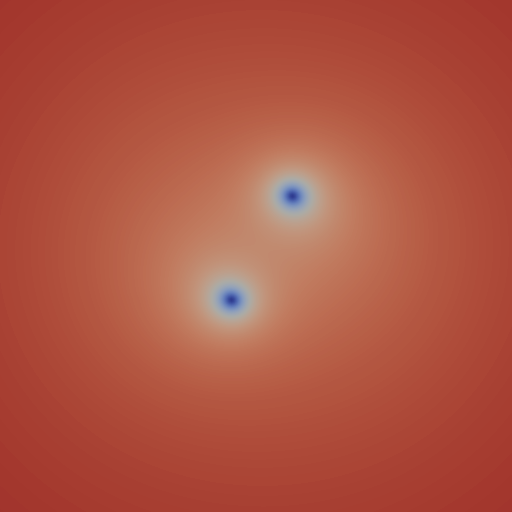
\includegraphics[width=4cm]{figs/gr_im1_r1.png}};
		\end{scope}
		%\begin{scope}[xshift=13.5cm,yshift=0.25cm]
		%\node[anchor=south west,inner sep=0] at (0,0) {\includegraphics[width=2cm]{figs/gr_im_r1.png}};
		%\end{scope}
		
		\begin{scope}[xshift=13.5cm,yshift=3.0cm,scale=0.063]
		\draw [gray, ultra thin] (0.000000, 64.000000) rectangle +(8.000000,-8.000000);
\draw [gray, ultra thin] (8.000000, 64.000000) rectangle +(8.000000,-8.000000);
\draw [gray, ultra thin] (16.000000, 64.000000) rectangle +(8.000000,-8.000000);
\draw [gray, ultra thin] (24.000000, 64.000000) rectangle +(8.000000,-8.000000);
\draw [gray, ultra thin] (32.000000, 64.000000) rectangle +(8.000000,-8.000000);
\draw [gray, ultra thin] (40.000000, 64.000000) rectangle +(8.000000,-8.000000);
\draw [gray, ultra thin] (48.000000, 64.000000) rectangle +(8.000000,-8.000000);
\draw [gray, ultra thin] (56.000000, 64.000000) rectangle +(8.000000,-8.000000);
\draw [gray, ultra thin] (0.000000, 56.000000) rectangle +(8.000000,-8.000000);
\draw [gray, ultra thin] (8.000000, 56.000000) rectangle +(4.000000,-4.000000);
\draw [gray, ultra thin] (12.000000, 56.000000) rectangle +(4.000000,-4.000000);
\draw [gray, ultra thin] (16.000000, 56.000000) rectangle +(4.000000,-4.000000);
\draw [gray, ultra thin] (20.000000, 56.000000) rectangle +(4.000000,-4.000000);
\draw [gray, ultra thin] (24.000000, 56.000000) rectangle +(4.000000,-4.000000);
\draw [gray, ultra thin] (28.000000, 56.000000) rectangle +(4.000000,-4.000000);
\draw [gray, ultra thin] (32.000000, 56.000000) rectangle +(4.000000,-4.000000);
\draw [gray, ultra thin] (36.000000, 56.000000) rectangle +(4.000000,-4.000000);
\draw [gray, ultra thin] (40.000000, 56.000000) rectangle +(4.000000,-4.000000);
\draw [gray, ultra thin] (44.000000, 56.000000) rectangle +(4.000000,-4.000000);
\draw [gray, ultra thin] (48.000000, 56.000000) rectangle +(4.000000,-4.000000);
\draw [gray, ultra thin] (52.000000, 56.000000) rectangle +(4.000000,-4.000000);
\draw [gray, ultra thin] (56.000000, 56.000000) rectangle +(8.000000,-8.000000);
\draw [gray, ultra thin] (8.000000, 52.000000) rectangle +(4.000000,-4.000000);
\draw [gray, ultra thin] (12.000000, 52.000000) rectangle +(4.000000,-4.000000);
\draw [gray, ultra thin] (16.000000, 52.000000) rectangle +(4.000000,-4.000000);
\draw [gray, ultra thin] (20.000000, 52.000000) rectangle +(4.000000,-4.000000);
\draw [gray, ultra thin] (24.000000, 52.000000) rectangle +(4.000000,-4.000000);
\draw [gray, ultra thin] (28.000000, 52.000000) rectangle +(4.000000,-4.000000);
\draw [gray, ultra thin] (32.000000, 52.000000) rectangle +(4.000000,-4.000000);
\draw [gray, ultra thin] (36.000000, 52.000000) rectangle +(4.000000,-4.000000);
\draw [gray, ultra thin] (40.000000, 52.000000) rectangle +(4.000000,-4.000000);
\draw [gray, ultra thin] (44.000000, 52.000000) rectangle +(4.000000,-4.000000);
\draw [gray, ultra thin] (48.000000, 52.000000) rectangle +(4.000000,-4.000000);
\draw [gray, ultra thin] (52.000000, 52.000000) rectangle +(4.000000,-4.000000);
\draw [gray, ultra thin] (0.000000, 48.000000) rectangle +(4.000000,-4.000000);
\draw [gray, ultra thin] (4.000000, 48.000000) rectangle +(4.000000,-4.000000);
\draw [gray, ultra thin] (8.000000, 48.000000) rectangle +(4.000000,-4.000000);
\draw [gray, ultra thin] (12.000000, 48.000000) rectangle +(4.000000,-4.000000);
\draw [gray, ultra thin] (16.000000, 48.000000) rectangle +(4.000000,-4.000000);
\draw [gray, ultra thin] (20.000000, 48.000000) rectangle +(2.000000,-2.000000);
\draw [gray, ultra thin] (22.000000, 48.000000) rectangle +(2.000000,-2.000000);
\draw [gray, ultra thin] (24.000000, 48.000000) rectangle +(4.000000,-4.000000);
\draw [gray, ultra thin] (28.000000, 48.000000) rectangle +(4.000000,-4.000000);
\draw [gray, ultra thin] (32.000000, 48.000000) rectangle +(4.000000,-4.000000);
\draw [gray, ultra thin] (36.000000, 48.000000) rectangle +(4.000000,-4.000000);
\draw [gray, ultra thin] (40.000000, 48.000000) rectangle +(2.000000,-2.000000);
\draw [gray, ultra thin] (42.000000, 48.000000) rectangle +(2.000000,-2.000000);
\draw [gray, ultra thin] (44.000000, 48.000000) rectangle +(4.000000,-4.000000);
\draw [gray, ultra thin] (48.000000, 48.000000) rectangle +(4.000000,-4.000000);
\draw [gray, ultra thin] (52.000000, 48.000000) rectangle +(4.000000,-4.000000);
\draw [gray, ultra thin] (56.000000, 48.000000) rectangle +(4.000000,-4.000000);
\draw [gray, ultra thin] (60.000000, 48.000000) rectangle +(4.000000,-4.000000);
\draw [gray, ultra thin] (20.000000, 46.000000) rectangle +(2.000000,-2.000000);
\draw [gray, ultra thin] (22.000000, 46.000000) rectangle +(2.000000,-2.000000);
\draw [gray, ultra thin] (40.000000, 46.000000) rectangle +(2.000000,-2.000000);
\draw [gray, ultra thin] (42.000000, 46.000000) rectangle +(2.000000,-2.000000);
\draw [gray, ultra thin] (0.000000, 44.000000) rectangle +(4.000000,-4.000000);
\draw [gray, ultra thin] (4.000000, 44.000000) rectangle +(4.000000,-4.000000);
\draw [gray, ultra thin] (8.000000, 44.000000) rectangle +(4.000000,-4.000000);
\draw [gray, ultra thin] (12.000000, 44.000000) rectangle +(2.000000,-2.000000);
\draw [gray, ultra thin] (14.000000, 44.000000) rectangle +(2.000000,-2.000000);
\draw [gray, ultra thin] (16.000000, 44.000000) rectangle +(2.000000,-2.000000);
\draw [gray, ultra thin] (18.000000, 44.000000) rectangle +(2.000000,-2.000000);
\draw [gray, ultra thin] (20.000000, 44.000000) rectangle +(2.000000,-2.000000);
\draw [gray, ultra thin] (22.000000, 44.000000) rectangle +(2.000000,-2.000000);
\draw [gray, ultra thin] (24.000000, 44.000000) rectangle +(2.000000,-2.000000);
\draw [gray, ultra thin] (26.000000, 44.000000) rectangle +(2.000000,-2.000000);
\draw [gray, ultra thin] (28.000000, 44.000000) rectangle +(4.000000,-4.000000);
\draw [gray, ultra thin] (32.000000, 44.000000) rectangle +(4.000000,-4.000000);
\draw [gray, ultra thin] (36.000000, 44.000000) rectangle +(2.000000,-2.000000);
\draw [gray, ultra thin] (38.000000, 44.000000) rectangle +(2.000000,-2.000000);
\draw [gray, ultra thin] (40.000000, 44.000000) rectangle +(2.000000,-2.000000);
\draw [gray, ultra thin] (42.000000, 44.000000) rectangle +(2.000000,-2.000000);
\draw [gray, ultra thin] (44.000000, 44.000000) rectangle +(2.000000,-2.000000);
\draw [gray, ultra thin] (46.000000, 44.000000) rectangle +(2.000000,-2.000000);
\draw [gray, ultra thin] (48.000000, 44.000000) rectangle +(2.000000,-2.000000);
\draw [gray, ultra thin] (50.000000, 44.000000) rectangle +(2.000000,-2.000000);
\draw [gray, ultra thin] (52.000000, 44.000000) rectangle +(4.000000,-4.000000);
\draw [gray, ultra thin] (56.000000, 44.000000) rectangle +(4.000000,-4.000000);
\draw [gray, ultra thin] (60.000000, 44.000000) rectangle +(4.000000,-4.000000);
\draw [gray, ultra thin] (12.000000, 42.000000) rectangle +(2.000000,-2.000000);
\draw [gray, ultra thin] (14.000000, 42.000000) rectangle +(2.000000,-2.000000);
\draw [gray, ultra thin] (16.000000, 42.000000) rectangle +(2.000000,-2.000000);
\draw [gray, ultra thin] (18.000000, 42.000000) rectangle +(2.000000,-2.000000);
\draw [gray, ultra thin] (20.000000, 42.000000) rectangle +(2.000000,-2.000000);
\draw [gray, ultra thin] (22.000000, 42.000000) rectangle +(2.000000,-2.000000);
\draw [gray, ultra thin] (24.000000, 42.000000) rectangle +(2.000000,-2.000000);
\draw [gray, ultra thin] (26.000000, 42.000000) rectangle +(2.000000,-2.000000);
\draw [gray, ultra thin] (36.000000, 42.000000) rectangle +(2.000000,-2.000000);
\draw [gray, ultra thin] (38.000000, 42.000000) rectangle +(2.000000,-2.000000);
\draw [gray, ultra thin] (40.000000, 42.000000) rectangle +(2.000000,-2.000000);
\draw [gray, ultra thin] (42.000000, 42.000000) rectangle +(2.000000,-2.000000);
\draw [gray, ultra thin] (44.000000, 42.000000) rectangle +(2.000000,-2.000000);
\draw [gray, ultra thin] (46.000000, 42.000000) rectangle +(2.000000,-2.000000);
\draw [gray, ultra thin] (48.000000, 42.000000) rectangle +(2.000000,-2.000000);
\draw [gray, ultra thin] (50.000000, 42.000000) rectangle +(2.000000,-2.000000);
\draw [gray, ultra thin] (0.000000, 40.000000) rectangle +(8.000000,-8.000000);
\draw [gray, ultra thin] (8.000000, 40.000000) rectangle +(4.000000,-4.000000);
\draw [gray, ultra thin] (12.000000, 40.000000) rectangle +(2.000000,-2.000000);
\draw [gray, ultra thin] (14.000000, 40.000000) rectangle +(2.000000,-2.000000);
\draw [gray, ultra thin] (16.000000, 40.000000) rectangle +(2.000000,-2.000000);
\draw [gray, ultra thin] (18.000000, 40.000000) rectangle +(2.000000,-2.000000);
\draw [gray, ultra thin] (20.000000, 40.000000) rectangle +(2.000000,-2.000000);
\draw [gray, ultra thin] (22.000000, 40.000000) rectangle +(2.000000,-2.000000);
\draw [gray, ultra thin] (24.000000, 40.000000) rectangle +(2.000000,-2.000000);
\draw [gray, ultra thin] (26.000000, 40.000000) rectangle +(2.000000,-2.000000);
\draw [gray, ultra thin] (28.000000, 40.000000) rectangle +(2.000000,-2.000000);
\draw [gray, ultra thin] (30.000000, 40.000000) rectangle +(2.000000,-2.000000);
\draw [gray, ultra thin] (32.000000, 40.000000) rectangle +(2.000000,-2.000000);
\draw [gray, ultra thin] (34.000000, 40.000000) rectangle +(2.000000,-2.000000);
\draw [gray, ultra thin] (36.000000, 40.000000) rectangle +(2.000000,-2.000000);
\draw [gray, ultra thin] (38.000000, 40.000000) rectangle +(2.000000,-2.000000);
\draw [gray, ultra thin] (40.000000, 40.000000) rectangle +(2.000000,-2.000000);
\draw [gray, ultra thin] (42.000000, 40.000000) rectangle +(2.000000,-2.000000);
\draw [gray, ultra thin] (44.000000, 40.000000) rectangle +(2.000000,-2.000000);
\draw [gray, ultra thin] (46.000000, 40.000000) rectangle +(2.000000,-2.000000);
\draw [gray, ultra thin] (48.000000, 40.000000) rectangle +(2.000000,-2.000000);
\draw [gray, ultra thin] (50.000000, 40.000000) rectangle +(2.000000,-2.000000);
\draw [gray, ultra thin] (52.000000, 40.000000) rectangle +(4.000000,-4.000000);
\draw [gray, ultra thin] (56.000000, 40.000000) rectangle +(4.000000,-4.000000);
\draw [gray, ultra thin] (60.000000, 40.000000) rectangle +(4.000000,-4.000000);
\draw [gray, ultra thin] (12.000000, 38.000000) rectangle +(2.000000,-2.000000);
\draw [gray, ultra thin] (14.000000, 38.000000) rectangle +(2.000000,-2.000000);
\draw [gray, ultra thin] (16.000000, 38.000000) rectangle +(2.000000,-2.000000);
\draw [gray, ultra thin] (18.000000, 38.000000) rectangle +(1.000000,-1.000000);
\draw [gray, ultra thin] (19.000000, 38.000000) rectangle +(1.000000,-1.000000);
\draw [gray, ultra thin] (20.000000, 38.000000) rectangle +(1.000000,-1.000000);
\draw [gray, ultra thin] (21.000000, 38.000000) rectangle +(1.000000,-1.000000);
\draw [gray, ultra thin] (22.000000, 38.000000) rectangle +(1.000000,-1.000000);
\draw [gray, ultra thin] (23.000000, 38.000000) rectangle +(1.000000,-1.000000);
\draw [gray, ultra thin] (24.000000, 38.000000) rectangle +(2.000000,-2.000000);
\draw [gray, ultra thin] (26.000000, 38.000000) rectangle +(2.000000,-2.000000);
\draw [gray, ultra thin] (28.000000, 38.000000) rectangle +(2.000000,-2.000000);
\draw [gray, ultra thin] (30.000000, 38.000000) rectangle +(2.000000,-2.000000);
\draw [gray, ultra thin] (32.000000, 38.000000) rectangle +(2.000000,-2.000000);
\draw [gray, ultra thin] (34.000000, 38.000000) rectangle +(2.000000,-2.000000);
\draw [gray, ultra thin] (36.000000, 38.000000) rectangle +(2.000000,-2.000000);
\draw [gray, ultra thin] (38.000000, 38.000000) rectangle +(2.000000,-2.000000);
\draw [gray, ultra thin] (40.000000, 38.000000) rectangle +(1.000000,-1.000000);
\draw [gray, ultra thin] (41.000000, 38.000000) rectangle +(1.000000,-1.000000);
\draw [gray, ultra thin] (42.000000, 38.000000) rectangle +(1.000000,-1.000000);
\draw [gray, ultra thin] (43.000000, 38.000000) rectangle +(1.000000,-1.000000);
\draw [gray, ultra thin] (44.000000, 38.000000) rectangle +(2.000000,-2.000000);
\draw [gray, ultra thin] (46.000000, 38.000000) rectangle +(2.000000,-2.000000);
\draw [gray, ultra thin] (48.000000, 38.000000) rectangle +(2.000000,-2.000000);
\draw [gray, ultra thin] (50.000000, 38.000000) rectangle +(2.000000,-2.000000);
\draw [gray, ultra thin] (18.000000, 37.000000) rectangle +(1.000000,-1.000000);
\draw [gray, ultra thin] (19.000000, 37.000000) rectangle +(1.000000,-1.000000);
\draw [gray, ultra thin] (20.000000, 37.000000) rectangle +(1.000000,-1.000000);
\draw [gray, ultra thin] (21.000000, 37.000000) rectangle +(1.000000,-1.000000);
\draw [gray, ultra thin] (22.000000, 37.000000) rectangle +(1.000000,-1.000000);
\draw [gray, ultra thin] (23.000000, 37.000000) rectangle +(1.000000,-1.000000);
\draw [gray, ultra thin] (40.000000, 37.000000) rectangle +(1.000000,-1.000000);
\draw [gray, ultra thin] (41.000000, 37.000000) rectangle +(1.000000,-1.000000);
\draw [gray, ultra thin] (42.000000, 37.000000) rectangle +(1.000000,-1.000000);
\draw [gray, ultra thin] (43.000000, 37.000000) rectangle +(1.000000,-1.000000);
\draw [gray, ultra thin] (8.000000, 36.000000) rectangle +(4.000000,-4.000000);
\draw [gray, ultra thin] (12.000000, 36.000000) rectangle +(2.000000,-2.000000);
\draw [gray, ultra thin] (14.000000, 36.000000) rectangle +(2.000000,-2.000000);
\draw [gray, ultra thin] (16.000000, 36.000000) rectangle +(1.000000,-1.000000);
\draw [gray, ultra thin] (17.000000, 36.000000) rectangle +(1.000000,-1.000000);
\draw [gray, ultra thin] (18.000000, 36.000000) rectangle +(1.000000,-1.000000);
\draw [gray, ultra thin] (19.000000, 36.000000) rectangle +(1.000000,-1.000000);
\draw [gray, ultra thin] (20.000000, 36.000000) rectangle +(1.000000,-1.000000);
\draw [gray, ultra thin] (21.000000, 36.000000) rectangle +(1.000000,-1.000000);
\draw [gray, ultra thin] (22.000000, 36.000000) rectangle +(2.000000,-2.000000);
\draw [gray, ultra thin] (24.000000, 36.000000) rectangle +(2.000000,-2.000000);
\draw [gray, ultra thin] (26.000000, 36.000000) rectangle +(2.000000,-2.000000);
\draw [gray, ultra thin] (28.000000, 36.000000) rectangle +(2.000000,-2.000000);
\draw [gray, ultra thin] (30.000000, 36.000000) rectangle +(2.000000,-2.000000);
\draw [gray, ultra thin] (32.000000, 36.000000) rectangle +(2.000000,-2.000000);
\draw [gray, ultra thin] (34.000000, 36.000000) rectangle +(2.000000,-2.000000);
\draw [gray, ultra thin] (36.000000, 36.000000) rectangle +(2.000000,-2.000000);
\draw [gray, ultra thin] (38.000000, 36.000000) rectangle +(2.000000,-2.000000);
\draw [gray, ultra thin] (40.000000, 36.000000) rectangle +(2.000000,-2.000000);
\draw [gray, ultra thin] (42.000000, 36.000000) rectangle +(1.000000,-1.000000);
\draw [gray, ultra thin] (43.000000, 36.000000) rectangle +(1.000000,-1.000000);
\draw [gray, ultra thin] (44.000000, 36.000000) rectangle +(1.000000,-1.000000);
\draw [gray, ultra thin] (45.000000, 36.000000) rectangle +(1.000000,-1.000000);
\draw [gray, ultra thin] (46.000000, 36.000000) rectangle +(2.000000,-2.000000);
\draw [gray, ultra thin] (48.000000, 36.000000) rectangle +(2.000000,-2.000000);
\draw [gray, ultra thin] (50.000000, 36.000000) rectangle +(2.000000,-2.000000);
\draw [gray, ultra thin] (52.000000, 36.000000) rectangle +(4.000000,-4.000000);
\draw [gray, ultra thin] (56.000000, 36.000000) rectangle +(4.000000,-4.000000);
\draw [gray, ultra thin] (60.000000, 36.000000) rectangle +(4.000000,-4.000000);
\draw [gray, ultra thin] (16.000000, 35.000000) rectangle +(1.000000,-1.000000);
\draw [gray, ultra thin] (17.000000, 35.000000) rectangle +(1.000000,-1.000000);
\draw [gray, ultra thin] (18.000000, 35.000000) rectangle +(1.000000,-1.000000);
\draw [gray, ultra thin] (19.000000, 35.000000) rectangle +(1.000000,-1.000000);
\draw [gray, ultra thin] (20.000000, 35.000000) rectangle +(1.000000,-1.000000);
\draw [gray, ultra thin] (21.000000, 35.000000) rectangle +(1.000000,-1.000000);
\draw [gray, ultra thin] (42.000000, 35.000000) rectangle +(1.000000,-1.000000);
\draw [gray, ultra thin] (43.000000, 35.000000) rectangle +(1.000000,-1.000000);
\draw [gray, ultra thin] (44.000000, 35.000000) rectangle +(1.000000,-1.000000);
\draw [gray, ultra thin] (45.000000, 35.000000) rectangle +(1.000000,-1.000000);
\draw [gray, ultra thin] (12.000000, 34.000000) rectangle +(2.000000,-2.000000);
\draw [gray, ultra thin] (14.000000, 34.000000) rectangle +(2.000000,-2.000000);
\draw [gray, ultra thin] (16.000000, 34.000000) rectangle +(2.000000,-2.000000);
\draw [gray, ultra thin] (18.000000, 34.000000) rectangle +(1.000000,-1.000000);
\draw [gray, ultra thin] (19.000000, 34.000000) rectangle +(1.000000,-1.000000);
\draw [gray, ultra thin] (20.000000, 34.000000) rectangle +(2.000000,-2.000000);
\draw [gray, ultra thin] (22.000000, 34.000000) rectangle +(0.500000,-0.500000);
\draw [gray, ultra thin] (22.500000, 34.000000) rectangle +(0.500000,-0.500000);
\draw [gray, ultra thin] (23.000000, 34.000000) rectangle +(0.500000,-0.500000);
\draw [gray, ultra thin] (23.500000, 34.000000) rectangle +(0.500000,-0.500000);
\draw [gray, ultra thin] (24.000000, 34.000000) rectangle +(0.500000,-0.500000);
\draw [gray, ultra thin] (24.500000, 34.000000) rectangle +(0.500000,-0.500000);
\draw [gray, ultra thin] (25.000000, 34.000000) rectangle +(0.500000,-0.500000);
\draw [gray, ultra thin] (25.500000, 34.000000) rectangle +(0.500000,-0.500000);
\draw [gray, ultra thin] (26.000000, 34.000000) rectangle +(2.000000,-2.000000);
\draw [gray, ultra thin] (28.000000, 34.000000) rectangle +(2.000000,-2.000000);
\draw [gray, ultra thin] (30.000000, 34.000000) rectangle +(2.000000,-2.000000);
\draw [gray, ultra thin] (32.000000, 34.000000) rectangle +(2.000000,-2.000000);
\draw [gray, ultra thin] (34.000000, 34.000000) rectangle +(2.000000,-2.000000);
\draw [gray, ultra thin] (36.000000, 34.000000) rectangle +(1.000000,-1.000000);
\draw [gray, ultra thin] (37.000000, 34.000000) rectangle +(1.000000,-1.000000);
\draw [gray, ultra thin] (38.000000, 34.000000) rectangle +(0.500000,-0.500000);
\draw [gray, ultra thin] (38.500000, 34.000000) rectangle +(0.500000,-0.500000);
\draw [gray, ultra thin] (39.000000, 34.000000) rectangle +(0.500000,-0.500000);
\draw [gray, ultra thin] (39.500000, 34.000000) rectangle +(0.500000,-0.500000);
\draw [gray, ultra thin] (40.000000, 34.000000) rectangle +(0.500000,-0.500000);
\draw [gray, ultra thin] (40.500000, 34.000000) rectangle +(0.500000,-0.500000);
\draw [gray, ultra thin] (41.000000, 34.000000) rectangle +(1.000000,-1.000000);
\draw [gray, ultra thin] (42.000000, 34.000000) rectangle +(2.000000,-2.000000);
\draw [gray, ultra thin] (44.000000, 34.000000) rectangle +(1.000000,-1.000000);
\draw [gray, ultra thin] (45.000000, 34.000000) rectangle +(1.000000,-1.000000);
\draw [gray, ultra thin] (46.000000, 34.000000) rectangle +(2.000000,-2.000000);
\draw [gray, ultra thin] (48.000000, 34.000000) rectangle +(2.000000,-2.000000);
\draw [gray, ultra thin] (50.000000, 34.000000) rectangle +(2.000000,-2.000000);
\draw [gray, ultra thin] (22.000000, 33.500000) rectangle +(0.500000,-0.500000);
\draw [gray, ultra thin] (22.500000, 33.500000) rectangle +(0.500000,-0.500000);
\draw [gray, ultra thin] (23.000000, 33.500000) rectangle +(0.250000,-0.250000);
\draw [gray, ultra thin] (23.250000, 33.500000) rectangle +(0.250000,-0.250000);
\draw [gray, ultra thin] (23.500000, 33.500000) rectangle +(0.250000,-0.250000);
\draw [gray, ultra thin] (23.750000, 33.500000) rectangle +(0.250000,-0.250000);
\draw [gray, ultra thin] (24.000000, 33.500000) rectangle +(0.500000,-0.500000);
\draw [gray, ultra thin] (24.500000, 33.500000) rectangle +(0.250000,-0.250000);
\draw [gray, ultra thin] (24.750000, 33.500000) rectangle +(0.250000,-0.250000);
\draw [gray, ultra thin] (25.000000, 33.500000) rectangle +(0.500000,-0.500000);
\draw [gray, ultra thin] (25.500000, 33.500000) rectangle +(0.500000,-0.500000);
\draw [gray, ultra thin] (38.000000, 33.500000) rectangle +(0.500000,-0.500000);
\draw [gray, ultra thin] (38.500000, 33.500000) rectangle +(0.500000,-0.500000);
\draw [gray, ultra thin] (39.000000, 33.500000) rectangle +(0.500000,-0.500000);
\draw [gray, ultra thin] (39.500000, 33.500000) rectangle +(0.250000,-0.250000);
\draw [gray, ultra thin] (39.750000, 33.500000) rectangle +(0.250000,-0.250000);
\draw [gray, ultra thin] (40.000000, 33.500000) rectangle +(0.250000,-0.250000);
\draw [gray, ultra thin] (40.250000, 33.500000) rectangle +(0.250000,-0.250000);
\draw [gray, ultra thin] (40.500000, 33.500000) rectangle +(0.500000,-0.500000);
\draw [gray, ultra thin] (23.000000, 33.250000) rectangle +(0.250000,-0.250000);
\draw [gray, ultra thin] (23.250000, 33.250000) rectangle +(0.250000,-0.250000);
\draw [gray, ultra thin] (23.500000, 33.250000) rectangle +(0.250000,-0.250000);
\draw [gray, ultra thin] (23.750000, 33.250000) rectangle +(0.250000,-0.250000);
\draw [gray, ultra thin] (24.500000, 33.250000) rectangle +(0.250000,-0.250000);
\draw [gray, ultra thin] (24.750000, 33.250000) rectangle +(0.250000,-0.250000);
\draw [gray, ultra thin] (39.500000, 33.250000) rectangle +(0.250000,-0.250000);
\draw [gray, ultra thin] (39.750000, 33.250000) rectangle +(0.250000,-0.250000);
\draw [gray, ultra thin] (40.000000, 33.250000) rectangle +(0.250000,-0.250000);
\draw [gray, ultra thin] (40.250000, 33.250000) rectangle +(0.250000,-0.250000);
\draw [gray, ultra thin] (18.000000, 33.000000) rectangle +(1.000000,-1.000000);
\draw [gray, ultra thin] (19.000000, 33.000000) rectangle +(1.000000,-1.000000);
\draw [gray, ultra thin] (22.000000, 33.000000) rectangle +(0.500000,-0.500000);
\draw [gray, ultra thin] (22.500000, 33.000000) rectangle +(0.250000,-0.250000);
\draw [gray, ultra thin] (22.750000, 33.000000) rectangle +(0.250000,-0.250000);
\draw [gray, ultra thin] (23.000000, 33.000000) rectangle +(0.250000,-0.250000);
\draw [gray, ultra thin] (23.250000, 33.000000) rectangle +(0.250000,-0.250000);
\draw [gray, ultra thin] (23.500000, 33.000000) rectangle +(0.250000,-0.250000);
\draw [gray, ultra thin] (23.750000, 33.000000) rectangle +(0.250000,-0.250000);
\draw [gray, ultra thin] (24.000000, 33.000000) rectangle +(0.250000,-0.250000);
\draw [gray, ultra thin] (24.250000, 33.000000) rectangle +(0.250000,-0.250000);
\draw [gray, ultra thin] (24.500000, 33.000000) rectangle +(0.250000,-0.250000);
\draw [gray, ultra thin] (24.750000, 33.000000) rectangle +(0.250000,-0.250000);
\draw [gray, ultra thin] (25.000000, 33.000000) rectangle +(0.250000,-0.250000);
\draw [gray, ultra thin] (25.250000, 33.000000) rectangle +(0.250000,-0.250000);
\draw [gray, ultra thin] (25.500000, 33.000000) rectangle +(0.500000,-0.500000);
\draw [gray, ultra thin] (36.000000, 33.000000) rectangle +(1.000000,-1.000000);
\draw [gray, ultra thin] (37.000000, 33.000000) rectangle +(0.500000,-0.500000);
\draw [gray, ultra thin] (37.500000, 33.000000) rectangle +(0.500000,-0.500000);
\draw [gray, ultra thin] (38.000000, 33.000000) rectangle +(0.250000,-0.250000);
\draw [gray, ultra thin] (38.250000, 33.000000) rectangle +(0.250000,-0.250000);
\draw [gray, ultra thin] (38.500000, 33.000000) rectangle +(0.250000,-0.250000);
\draw [gray, ultra thin] (38.750000, 33.000000) rectangle +(0.250000,-0.250000);
\draw [gray, ultra thin] (39.000000, 33.000000) rectangle +(0.250000,-0.250000);
\draw [gray, ultra thin] (39.250000, 33.000000) rectangle +(0.250000,-0.250000);
\draw [gray, ultra thin] (39.500000, 33.000000) rectangle +(0.250000,-0.250000);
\draw [gray, ultra thin] (39.750000, 33.000000) rectangle +(0.250000,-0.250000);
\draw [gray, ultra thin] (40.000000, 33.000000) rectangle +(0.250000,-0.250000);
\draw [gray, ultra thin] (40.250000, 33.000000) rectangle +(0.250000,-0.250000);
\draw [gray, ultra thin] (40.500000, 33.000000) rectangle +(0.250000,-0.250000);
\draw [gray, ultra thin] (40.750000, 33.000000) rectangle +(0.250000,-0.250000);
\draw [gray, ultra thin] (41.000000, 33.000000) rectangle +(0.500000,-0.500000);
\draw [gray, ultra thin] (41.500000, 33.000000) rectangle +(0.500000,-0.500000);
\draw [gray, ultra thin] (44.000000, 33.000000) rectangle +(1.000000,-1.000000);
\draw [gray, ultra thin] (45.000000, 33.000000) rectangle +(1.000000,-1.000000);
\draw [gray, ultra thin] (22.500000, 32.750000) rectangle +(0.250000,-0.250000);
\draw [gray, ultra thin] (22.750000, 32.750000) rectangle +(0.250000,-0.250000);
\draw [gray, ultra thin] (23.000000, 32.750000) rectangle +(0.250000,-0.250000);
\draw [gray, ultra thin] (23.250000, 32.750000) rectangle +(0.250000,-0.250000);
\draw [gray, ultra thin] (23.500000, 32.750000) rectangle +(0.250000,-0.250000);
\draw [gray, ultra thin] (23.750000, 32.750000) rectangle +(0.250000,-0.250000);
\draw [gray, ultra thin] (24.000000, 32.750000) rectangle +(0.250000,-0.250000);
\draw [gray, ultra thin] (24.250000, 32.750000) rectangle +(0.250000,-0.250000);
\draw [gray, ultra thin] (24.500000, 32.750000) rectangle +(0.250000,-0.250000);
\draw [gray, ultra thin] (24.750000, 32.750000) rectangle +(0.250000,-0.250000);
\draw [gray, ultra thin] (25.000000, 32.750000) rectangle +(0.250000,-0.250000);
\draw [gray, ultra thin] (25.250000, 32.750000) rectangle +(0.250000,-0.250000);
\draw [gray, ultra thin] (38.000000, 32.750000) rectangle +(0.250000,-0.250000);
\draw [gray, ultra thin] (38.250000, 32.750000) rectangle +(0.250000,-0.250000);
\draw [gray, ultra thin] (38.500000, 32.750000) rectangle +(0.250000,-0.250000);
\draw [gray, ultra thin] (38.750000, 32.750000) rectangle +(0.250000,-0.250000);
\draw [gray, ultra thin] (39.000000, 32.750000) rectangle +(0.250000,-0.250000);
\draw [gray, ultra thin] (39.250000, 32.750000) rectangle +(0.250000,-0.250000);
\draw [gray, ultra thin] (39.500000, 32.750000) rectangle +(0.250000,-0.250000);
\draw [gray, ultra thin] (39.750000, 32.750000) rectangle +(0.250000,-0.250000);
\draw [gray, ultra thin] (40.000000, 32.750000) rectangle +(0.250000,-0.250000);
\draw [gray, ultra thin] (40.250000, 32.750000) rectangle +(0.250000,-0.250000);
\draw [gray, ultra thin] (40.500000, 32.750000) rectangle +(0.250000,-0.250000);
\draw [gray, ultra thin] (40.750000, 32.750000) rectangle +(0.250000,-0.250000);
\draw [gray, ultra thin] (22.000000, 32.500000) rectangle +(0.500000,-0.500000);
\draw [gray, ultra thin] (22.500000, 32.500000) rectangle +(0.250000,-0.250000);
\draw [gray, ultra thin] (22.750000, 32.500000) rectangle +(0.250000,-0.250000);
\draw [gray, ultra thin] (23.000000, 32.500000) rectangle +(0.250000,-0.250000);
\draw [gray, ultra thin] (23.250000, 32.500000) rectangle +(0.250000,-0.250000);
\draw [gray, ultra thin] (23.500000, 32.500000) rectangle +(0.250000,-0.250000);
\draw [gray, ultra thin] (23.750000, 32.500000) rectangle +(0.250000,-0.250000);
\draw [gray, ultra thin] (24.000000, 32.500000) rectangle +(0.250000,-0.250000);
\draw [gray, ultra thin] (24.250000, 32.500000) rectangle +(0.250000,-0.250000);
\draw [gray, ultra thin] (24.500000, 32.500000) rectangle +(0.250000,-0.250000);
\draw [gray, ultra thin] (24.750000, 32.500000) rectangle +(0.250000,-0.250000);
\draw [gray, ultra thin] (25.000000, 32.500000) rectangle +(0.250000,-0.250000);
\draw [gray, ultra thin] (25.250000, 32.500000) rectangle +(0.250000,-0.250000);
\draw [gray, ultra thin] (25.500000, 32.500000) rectangle +(0.500000,-0.500000);
\draw [gray, ultra thin] (37.000000, 32.500000) rectangle +(0.500000,-0.500000);
\draw [gray, ultra thin] (37.500000, 32.500000) rectangle +(0.500000,-0.500000);
\draw [gray, ultra thin] (38.000000, 32.500000) rectangle +(0.250000,-0.250000);
\draw [gray, ultra thin] (38.250000, 32.500000) rectangle +(0.250000,-0.250000);
\draw [gray, ultra thin] (38.500000, 32.500000) rectangle +(0.250000,-0.250000);
\draw [gray, ultra thin] (38.750000, 32.500000) rectangle +(0.250000,-0.250000);
\draw [gray, ultra thin] (39.000000, 32.500000) rectangle +(0.250000,-0.250000);
\draw [gray, ultra thin] (39.250000, 32.500000) rectangle +(0.250000,-0.250000);
\draw [gray, ultra thin] (39.500000, 32.500000) rectangle +(0.250000,-0.250000);
\draw [gray, ultra thin] (39.750000, 32.500000) rectangle +(0.250000,-0.250000);
\draw [gray, ultra thin] (40.000000, 32.500000) rectangle +(0.250000,-0.250000);
\draw [gray, ultra thin] (40.250000, 32.500000) rectangle +(0.250000,-0.250000);
\draw [gray, ultra thin] (40.500000, 32.500000) rectangle +(0.250000,-0.250000);
\draw [gray, ultra thin] (40.750000, 32.500000) rectangle +(0.250000,-0.250000);
\draw [gray, ultra thin] (41.000000, 32.500000) rectangle +(0.500000,-0.500000);
\draw [gray, ultra thin] (41.500000, 32.500000) rectangle +(0.500000,-0.500000);
\draw [gray, ultra thin] (22.500000, 32.250000) rectangle +(0.250000,-0.250000);
\draw [gray, ultra thin] (22.750000, 32.250000) rectangle +(0.250000,-0.250000);
\draw [gray, ultra thin] (23.000000, 32.250000) rectangle +(0.250000,-0.250000);
\draw [gray, ultra thin] (23.250000, 32.250000) rectangle +(0.250000,-0.250000);
\draw [gray, ultra thin] (23.500000, 32.250000) rectangle +(0.125000,-0.125000);
\draw [gray, ultra thin] (23.625000, 32.250000) rectangle +(0.125000,-0.125000);
\draw [gray, ultra thin] (23.750000, 32.250000) rectangle +(0.250000,-0.250000);
\draw [gray, ultra thin] (24.000000, 32.250000) rectangle +(0.250000,-0.250000);
\draw [gray, ultra thin] (24.250000, 32.250000) rectangle +(0.125000,-0.125000);
\draw [gray, ultra thin] (24.375000, 32.250000) rectangle +(0.125000,-0.125000);
\draw [gray, ultra thin] (24.500000, 32.250000) rectangle +(0.250000,-0.250000);
\draw [gray, ultra thin] (24.750000, 32.250000) rectangle +(0.250000,-0.250000);
\draw [gray, ultra thin] (25.000000, 32.250000) rectangle +(0.250000,-0.250000);
\draw [gray, ultra thin] (25.250000, 32.250000) rectangle +(0.250000,-0.250000);
\draw [gray, ultra thin] (38.000000, 32.250000) rectangle +(0.250000,-0.250000);
\draw [gray, ultra thin] (38.250000, 32.250000) rectangle +(0.250000,-0.250000);
\draw [gray, ultra thin] (38.500000, 32.250000) rectangle +(0.250000,-0.250000);
\draw [gray, ultra thin] (38.750000, 32.250000) rectangle +(0.250000,-0.250000);
\draw [gray, ultra thin] (39.000000, 32.250000) rectangle +(0.125000,-0.125000);
\draw [gray, ultra thin] (39.125000, 32.250000) rectangle +(0.125000,-0.125000);
\draw [gray, ultra thin] (39.250000, 32.250000) rectangle +(0.250000,-0.250000);
\draw [gray, ultra thin] (39.500000, 32.250000) rectangle +(0.250000,-0.250000);
\draw [gray, ultra thin] (39.750000, 32.250000) rectangle +(0.125000,-0.125000);
\draw [gray, ultra thin] (39.875000, 32.250000) rectangle +(0.125000,-0.125000);
\draw [gray, ultra thin] (40.000000, 32.250000) rectangle +(0.250000,-0.250000);
\draw [gray, ultra thin] (40.250000, 32.250000) rectangle +(0.250000,-0.250000);
\draw [gray, ultra thin] (40.500000, 32.250000) rectangle +(0.250000,-0.250000);
\draw [gray, ultra thin] (40.750000, 32.250000) rectangle +(0.250000,-0.250000);
\draw [gray, ultra thin] (23.500000, 32.125000) rectangle +(0.125000,-0.125000);
\draw [gray, ultra thin] (23.625000, 32.125000) rectangle +(0.125000,-0.125000);
\draw [gray, ultra thin] (24.250000, 32.125000) rectangle +(0.125000,-0.125000);
\draw [gray, ultra thin] (24.375000, 32.125000) rectangle +(0.125000,-0.125000);
\draw [gray, ultra thin] (39.000000, 32.125000) rectangle +(0.125000,-0.125000);
\draw [gray, ultra thin] (39.125000, 32.125000) rectangle +(0.125000,-0.125000);
\draw [gray, ultra thin] (39.750000, 32.125000) rectangle +(0.125000,-0.125000);
\draw [gray, ultra thin] (39.875000, 32.125000) rectangle +(0.125000,-0.125000);
\draw [gray, ultra thin] (0.000000, 32.000000) rectangle +(8.000000,-8.000000);
\draw [gray, ultra thin] (8.000000, 32.000000) rectangle +(4.000000,-4.000000);
\draw [gray, ultra thin] (12.000000, 32.000000) rectangle +(2.000000,-2.000000);
\draw [gray, ultra thin] (14.000000, 32.000000) rectangle +(2.000000,-2.000000);
\draw [gray, ultra thin] (16.000000, 32.000000) rectangle +(2.000000,-2.000000);
\draw [gray, ultra thin] (18.000000, 32.000000) rectangle +(1.000000,-1.000000);
\draw [gray, ultra thin] (19.000000, 32.000000) rectangle +(1.000000,-1.000000);
\draw [gray, ultra thin] (20.000000, 32.000000) rectangle +(2.000000,-2.000000);
\draw [gray, ultra thin] (22.000000, 32.000000) rectangle +(0.500000,-0.500000);
\draw [gray, ultra thin] (22.500000, 32.000000) rectangle +(0.250000,-0.250000);
\draw [gray, ultra thin] (22.750000, 32.000000) rectangle +(0.250000,-0.250000);
\draw [gray, ultra thin] (23.000000, 32.000000) rectangle +(0.250000,-0.250000);
\draw [gray, ultra thin] (23.250000, 32.000000) rectangle +(0.125000,-0.125000);
\draw [gray, ultra thin] (23.375000, 32.000000) rectangle +(0.125000,-0.125000);
\draw [gray, ultra thin] (23.500000, 32.000000) rectangle +(0.250000,-0.250000);
\draw [gray, ultra thin] (23.750000, 32.000000) rectangle +(0.250000,-0.250000);
\draw [gray, ultra thin] (24.000000, 32.000000) rectangle +(0.250000,-0.250000);
\draw [gray, ultra thin] (24.250000, 32.000000) rectangle +(0.125000,-0.125000);
\draw [gray, ultra thin] (24.375000, 32.000000) rectangle +(0.125000,-0.125000);
\draw [gray, ultra thin] (24.500000, 32.000000) rectangle +(0.250000,-0.250000);
\draw [gray, ultra thin] (24.750000, 32.000000) rectangle +(0.250000,-0.250000);
\draw [gray, ultra thin] (25.000000, 32.000000) rectangle +(0.250000,-0.250000);
\draw [gray, ultra thin] (25.250000, 32.000000) rectangle +(0.250000,-0.250000);
\draw [gray, ultra thin] (25.500000, 32.000000) rectangle +(0.500000,-0.500000);
\draw [gray, ultra thin] (26.000000, 32.000000) rectangle +(2.000000,-2.000000);
\draw [gray, ultra thin] (28.000000, 32.000000) rectangle +(4.000000,-4.000000);
\draw [gray, ultra thin] (32.000000, 32.000000) rectangle +(4.000000,-4.000000);
\draw [gray, ultra thin] (36.000000, 32.000000) rectangle +(1.000000,-1.000000);
\draw [gray, ultra thin] (37.000000, 32.000000) rectangle +(0.500000,-0.500000);
\draw [gray, ultra thin] (37.500000, 32.000000) rectangle +(0.500000,-0.500000);
\draw [gray, ultra thin] (38.000000, 32.000000) rectangle +(0.250000,-0.250000);
\draw [gray, ultra thin] (38.250000, 32.000000) rectangle +(0.250000,-0.250000);
\draw [gray, ultra thin] (38.500000, 32.000000) rectangle +(0.250000,-0.250000);
\draw [gray, ultra thin] (38.750000, 32.000000) rectangle +(0.250000,-0.250000);
\draw [gray, ultra thin] (39.000000, 32.000000) rectangle +(0.125000,-0.125000);
\draw [gray, ultra thin] (39.125000, 32.000000) rectangle +(0.125000,-0.125000);
\draw [gray, ultra thin] (39.250000, 32.000000) rectangle +(0.250000,-0.250000);
\draw [gray, ultra thin] (39.500000, 32.000000) rectangle +(0.250000,-0.250000);
\draw [gray, ultra thin] (39.750000, 32.000000) rectangle +(0.250000,-0.250000);
\draw [gray, ultra thin] (40.000000, 32.000000) rectangle +(0.250000,-0.250000);
\draw [gray, ultra thin] (40.250000, 32.000000) rectangle +(0.250000,-0.250000);
\draw [gray, ultra thin] (40.500000, 32.000000) rectangle +(0.250000,-0.250000);
\draw [gray, ultra thin] (40.750000, 32.000000) rectangle +(0.250000,-0.250000);
\draw [gray, ultra thin] (41.000000, 32.000000) rectangle +(0.500000,-0.500000);
\draw [gray, ultra thin] (41.500000, 32.000000) rectangle +(0.500000,-0.500000);
\draw [gray, ultra thin] (42.000000, 32.000000) rectangle +(2.000000,-2.000000);
\draw [gray, ultra thin] (44.000000, 32.000000) rectangle +(1.000000,-1.000000);
\draw [gray, ultra thin] (45.000000, 32.000000) rectangle +(1.000000,-1.000000);
\draw [gray, ultra thin] (46.000000, 32.000000) rectangle +(2.000000,-2.000000);
\draw [gray, ultra thin] (48.000000, 32.000000) rectangle +(2.000000,-2.000000);
\draw [gray, ultra thin] (50.000000, 32.000000) rectangle +(2.000000,-2.000000);
\draw [gray, ultra thin] (52.000000, 32.000000) rectangle +(4.000000,-4.000000);
\draw [gray, ultra thin] (56.000000, 32.000000) rectangle +(4.000000,-4.000000);
\draw [gray, ultra thin] (60.000000, 32.000000) rectangle +(4.000000,-4.000000);
\draw [gray, ultra thin] (23.250000, 31.875000) rectangle +(0.125000,-0.125000);
\draw [gray, ultra thin] (23.375000, 31.875000) rectangle +(0.125000,-0.125000);
\draw [gray, ultra thin] (24.250000, 31.875000) rectangle +(0.125000,-0.125000);
\draw [gray, ultra thin] (24.375000, 31.875000) rectangle +(0.125000,-0.125000);
\draw [gray, ultra thin] (39.000000, 31.875000) rectangle +(0.125000,-0.125000);
\draw [gray, ultra thin] (39.125000, 31.875000) rectangle +(0.125000,-0.125000);
\draw [gray, ultra thin] (22.500000, 31.750000) rectangle +(0.250000,-0.250000);
\draw [gray, ultra thin] (22.750000, 31.750000) rectangle +(0.250000,-0.250000);
\draw [gray, ultra thin] (23.000000, 31.750000) rectangle +(0.250000,-0.250000);
\draw [gray, ultra thin] (23.250000, 31.750000) rectangle +(0.250000,-0.250000);
\draw [gray, ultra thin] (23.500000, 31.750000) rectangle +(0.250000,-0.250000);
\draw [gray, ultra thin] (23.750000, 31.750000) rectangle +(0.250000,-0.250000);
\draw [gray, ultra thin] (24.000000, 31.750000) rectangle +(0.250000,-0.250000);
\draw [gray, ultra thin] (24.250000, 31.750000) rectangle +(0.250000,-0.250000);
\draw [gray, ultra thin] (24.500000, 31.750000) rectangle +(0.250000,-0.250000);
\draw [gray, ultra thin] (24.750000, 31.750000) rectangle +(0.250000,-0.250000);
\draw [gray, ultra thin] (25.000000, 31.750000) rectangle +(0.250000,-0.250000);
\draw [gray, ultra thin] (25.250000, 31.750000) rectangle +(0.250000,-0.250000);
\draw [gray, ultra thin] (38.000000, 31.750000) rectangle +(0.250000,-0.250000);
\draw [gray, ultra thin] (38.250000, 31.750000) rectangle +(0.250000,-0.250000);
\draw [gray, ultra thin] (38.500000, 31.750000) rectangle +(0.250000,-0.250000);
\draw [gray, ultra thin] (38.750000, 31.750000) rectangle +(0.250000,-0.250000);
\draw [gray, ultra thin] (39.000000, 31.750000) rectangle +(0.250000,-0.250000);
\draw [gray, ultra thin] (39.250000, 31.750000) rectangle +(0.250000,-0.250000);
\draw [gray, ultra thin] (39.500000, 31.750000) rectangle +(0.250000,-0.250000);
\draw [gray, ultra thin] (39.750000, 31.750000) rectangle +(0.250000,-0.250000);
\draw [gray, ultra thin] (40.000000, 31.750000) rectangle +(0.250000,-0.250000);
\draw [gray, ultra thin] (40.250000, 31.750000) rectangle +(0.250000,-0.250000);
\draw [gray, ultra thin] (40.500000, 31.750000) rectangle +(0.250000,-0.250000);
\draw [gray, ultra thin] (40.750000, 31.750000) rectangle +(0.250000,-0.250000);
\draw [gray, ultra thin] (22.000000, 31.500000) rectangle +(0.500000,-0.500000);
\draw [gray, ultra thin] (22.500000, 31.500000) rectangle +(0.250000,-0.250000);
\draw [gray, ultra thin] (22.750000, 31.500000) rectangle +(0.250000,-0.250000);
\draw [gray, ultra thin] (23.000000, 31.500000) rectangle +(0.250000,-0.250000);
\draw [gray, ultra thin] (23.250000, 31.500000) rectangle +(0.250000,-0.250000);
\draw [gray, ultra thin] (23.500000, 31.500000) rectangle +(0.250000,-0.250000);
\draw [gray, ultra thin] (23.750000, 31.500000) rectangle +(0.250000,-0.250000);
\draw [gray, ultra thin] (24.000000, 31.500000) rectangle +(0.250000,-0.250000);
\draw [gray, ultra thin] (24.250000, 31.500000) rectangle +(0.125000,-0.125000);
\draw [gray, ultra thin] (24.375000, 31.500000) rectangle +(0.125000,-0.125000);
\draw [gray, ultra thin] (24.500000, 31.500000) rectangle +(0.250000,-0.250000);
\draw [gray, ultra thin] (24.750000, 31.500000) rectangle +(0.250000,-0.250000);
\draw [gray, ultra thin] (25.000000, 31.500000) rectangle +(0.250000,-0.250000);
\draw [gray, ultra thin] (25.250000, 31.500000) rectangle +(0.250000,-0.250000);
\draw [gray, ultra thin] (25.500000, 31.500000) rectangle +(0.500000,-0.500000);
\draw [gray, ultra thin] (37.000000, 31.500000) rectangle +(0.500000,-0.500000);
\draw [gray, ultra thin] (37.500000, 31.500000) rectangle +(0.500000,-0.500000);
\draw [gray, ultra thin] (38.000000, 31.500000) rectangle +(0.250000,-0.250000);
\draw [gray, ultra thin] (38.250000, 31.500000) rectangle +(0.250000,-0.250000);
\draw [gray, ultra thin] (38.500000, 31.500000) rectangle +(0.250000,-0.250000);
\draw [gray, ultra thin] (38.750000, 31.500000) rectangle +(0.250000,-0.250000);
\draw [gray, ultra thin] (39.000000, 31.500000) rectangle +(0.125000,-0.125000);
\draw [gray, ultra thin] (39.125000, 31.500000) rectangle +(0.125000,-0.125000);
\draw [gray, ultra thin] (39.250000, 31.500000) rectangle +(0.250000,-0.250000);
\draw [gray, ultra thin] (39.500000, 31.500000) rectangle +(0.250000,-0.250000);
\draw [gray, ultra thin] (39.750000, 31.500000) rectangle +(0.250000,-0.250000);
\draw [gray, ultra thin] (40.000000, 31.500000) rectangle +(0.125000,-0.125000);
\draw [gray, ultra thin] (40.125000, 31.500000) rectangle +(0.125000,-0.125000);
\draw [gray, ultra thin] (40.250000, 31.500000) rectangle +(0.250000,-0.250000);
\draw [gray, ultra thin] (40.500000, 31.500000) rectangle +(0.250000,-0.250000);
\draw [gray, ultra thin] (40.750000, 31.500000) rectangle +(0.250000,-0.250000);
\draw [gray, ultra thin] (41.000000, 31.500000) rectangle +(0.500000,-0.500000);
\draw [gray, ultra thin] (41.500000, 31.500000) rectangle +(0.500000,-0.500000);
\draw [gray, ultra thin] (24.250000, 31.375000) rectangle +(0.125000,-0.125000);
\draw [gray, ultra thin] (24.375000, 31.375000) rectangle +(0.125000,-0.125000);
\draw [gray, ultra thin] (39.000000, 31.375000) rectangle +(0.125000,-0.125000);
\draw [gray, ultra thin] (39.125000, 31.375000) rectangle +(0.125000,-0.125000);
\draw [gray, ultra thin] (40.000000, 31.375000) rectangle +(0.125000,-0.125000);
\draw [gray, ultra thin] (40.125000, 31.375000) rectangle +(0.125000,-0.125000);
\draw [gray, ultra thin] (22.500000, 31.250000) rectangle +(0.250000,-0.250000);
\draw [gray, ultra thin] (22.750000, 31.250000) rectangle +(0.250000,-0.250000);
\draw [gray, ultra thin] (23.000000, 31.250000) rectangle +(0.250000,-0.250000);
\draw [gray, ultra thin] (23.250000, 31.250000) rectangle +(0.250000,-0.250000);
\draw [gray, ultra thin] (23.500000, 31.250000) rectangle +(0.125000,-0.125000);
\draw [gray, ultra thin] (23.625000, 31.250000) rectangle +(0.125000,-0.125000);
\draw [gray, ultra thin] (23.750000, 31.250000) rectangle +(0.250000,-0.250000);
\draw [gray, ultra thin] (24.000000, 31.250000) rectangle +(0.250000,-0.250000);
\draw [gray, ultra thin] (24.250000, 31.250000) rectangle +(0.125000,-0.125000);
\draw [gray, ultra thin] (24.375000, 31.250000) rectangle +(0.125000,-0.125000);
\draw [gray, ultra thin] (24.500000, 31.250000) rectangle +(0.250000,-0.250000);
\draw [gray, ultra thin] (24.750000, 31.250000) rectangle +(0.250000,-0.250000);
\draw [gray, ultra thin] (25.000000, 31.250000) rectangle +(0.250000,-0.250000);
\draw [gray, ultra thin] (25.250000, 31.250000) rectangle +(0.250000,-0.250000);
\draw [gray, ultra thin] (38.000000, 31.250000) rectangle +(0.250000,-0.250000);
\draw [gray, ultra thin] (38.250000, 31.250000) rectangle +(0.250000,-0.250000);
\draw [gray, ultra thin] (38.500000, 31.250000) rectangle +(0.250000,-0.250000);
\draw [gray, ultra thin] (38.750000, 31.250000) rectangle +(0.250000,-0.250000);
\draw [gray, ultra thin] (39.000000, 31.250000) rectangle +(0.125000,-0.125000);
\draw [gray, ultra thin] (39.125000, 31.250000) rectangle +(0.125000,-0.125000);
\draw [gray, ultra thin] (39.250000, 31.250000) rectangle +(0.250000,-0.250000);
\draw [gray, ultra thin] (39.500000, 31.250000) rectangle +(0.250000,-0.250000);
\draw [gray, ultra thin] (39.750000, 31.250000) rectangle +(0.125000,-0.125000);
\draw [gray, ultra thin] (39.875000, 31.250000) rectangle +(0.125000,-0.125000);
\draw [gray, ultra thin] (40.000000, 31.250000) rectangle +(0.250000,-0.250000);
\draw [gray, ultra thin] (40.250000, 31.250000) rectangle +(0.250000,-0.250000);
\draw [gray, ultra thin] (40.500000, 31.250000) rectangle +(0.250000,-0.250000);
\draw [gray, ultra thin] (40.750000, 31.250000) rectangle +(0.250000,-0.250000);
\draw [gray, ultra thin] (23.500000, 31.125000) rectangle +(0.125000,-0.125000);
\draw [gray, ultra thin] (23.625000, 31.125000) rectangle +(0.125000,-0.125000);
\draw [gray, ultra thin] (24.250000, 31.125000) rectangle +(0.125000,-0.125000);
\draw [gray, ultra thin] (24.375000, 31.125000) rectangle +(0.125000,-0.125000);
\draw [gray, ultra thin] (39.000000, 31.125000) rectangle +(0.125000,-0.125000);
\draw [gray, ultra thin] (39.125000, 31.125000) rectangle +(0.125000,-0.125000);
\draw [gray, ultra thin] (39.750000, 31.125000) rectangle +(0.125000,-0.125000);
\draw [gray, ultra thin] (39.875000, 31.125000) rectangle +(0.125000,-0.125000);
\draw [gray, ultra thin] (18.000000, 31.000000) rectangle +(1.000000,-1.000000);
\draw [gray, ultra thin] (19.000000, 31.000000) rectangle +(1.000000,-1.000000);
\draw [gray, ultra thin] (22.000000, 31.000000) rectangle +(0.500000,-0.500000);
\draw [gray, ultra thin] (22.500000, 31.000000) rectangle +(0.250000,-0.250000);
\draw [gray, ultra thin] (22.750000, 31.000000) rectangle +(0.250000,-0.250000);
\draw [gray, ultra thin] (23.000000, 31.000000) rectangle +(0.250000,-0.250000);
\draw [gray, ultra thin] (23.250000, 31.000000) rectangle +(0.250000,-0.250000);
\draw [gray, ultra thin] (23.500000, 31.000000) rectangle +(0.250000,-0.250000);
\draw [gray, ultra thin] (23.750000, 31.000000) rectangle +(0.250000,-0.250000);
\draw [gray, ultra thin] (24.000000, 31.000000) rectangle +(0.250000,-0.250000);
\draw [gray, ultra thin] (24.250000, 31.000000) rectangle +(0.250000,-0.250000);
\draw [gray, ultra thin] (24.500000, 31.000000) rectangle +(0.250000,-0.250000);
\draw [gray, ultra thin] (24.750000, 31.000000) rectangle +(0.250000,-0.250000);
\draw [gray, ultra thin] (25.000000, 31.000000) rectangle +(0.250000,-0.250000);
\draw [gray, ultra thin] (25.250000, 31.000000) rectangle +(0.250000,-0.250000);
\draw [gray, ultra thin] (25.500000, 31.000000) rectangle +(0.500000,-0.500000);
\draw [gray, ultra thin] (36.000000, 31.000000) rectangle +(1.000000,-1.000000);
\draw [gray, ultra thin] (37.000000, 31.000000) rectangle +(0.500000,-0.500000);
\draw [gray, ultra thin] (37.500000, 31.000000) rectangle +(0.500000,-0.500000);
\draw [gray, ultra thin] (38.000000, 31.000000) rectangle +(0.250000,-0.250000);
\draw [gray, ultra thin] (38.250000, 31.000000) rectangle +(0.250000,-0.250000);
\draw [gray, ultra thin] (38.500000, 31.000000) rectangle +(0.250000,-0.250000);
\draw [gray, ultra thin] (38.750000, 31.000000) rectangle +(0.250000,-0.250000);
\draw [gray, ultra thin] (39.000000, 31.000000) rectangle +(0.250000,-0.250000);
\draw [gray, ultra thin] (39.250000, 31.000000) rectangle +(0.250000,-0.250000);
\draw [gray, ultra thin] (39.500000, 31.000000) rectangle +(0.250000,-0.250000);
\draw [gray, ultra thin] (39.750000, 31.000000) rectangle +(0.250000,-0.250000);
\draw [gray, ultra thin] (40.000000, 31.000000) rectangle +(0.250000,-0.250000);
\draw [gray, ultra thin] (40.250000, 31.000000) rectangle +(0.250000,-0.250000);
\draw [gray, ultra thin] (40.500000, 31.000000) rectangle +(0.250000,-0.250000);
\draw [gray, ultra thin] (40.750000, 31.000000) rectangle +(0.250000,-0.250000);
\draw [gray, ultra thin] (41.000000, 31.000000) rectangle +(0.500000,-0.500000);
\draw [gray, ultra thin] (41.500000, 31.000000) rectangle +(0.500000,-0.500000);
\draw [gray, ultra thin] (44.000000, 31.000000) rectangle +(1.000000,-1.000000);
\draw [gray, ultra thin] (45.000000, 31.000000) rectangle +(1.000000,-1.000000);
\draw [gray, ultra thin] (22.500000, 30.750000) rectangle +(0.250000,-0.250000);
\draw [gray, ultra thin] (22.750000, 30.750000) rectangle +(0.250000,-0.250000);
\draw [gray, ultra thin] (23.000000, 30.750000) rectangle +(0.250000,-0.250000);
\draw [gray, ultra thin] (23.250000, 30.750000) rectangle +(0.250000,-0.250000);
\draw [gray, ultra thin] (23.500000, 30.750000) rectangle +(0.250000,-0.250000);
\draw [gray, ultra thin] (23.750000, 30.750000) rectangle +(0.250000,-0.250000);
\draw [gray, ultra thin] (24.000000, 30.750000) rectangle +(0.250000,-0.250000);
\draw [gray, ultra thin] (24.250000, 30.750000) rectangle +(0.250000,-0.250000);
\draw [gray, ultra thin] (24.500000, 30.750000) rectangle +(0.250000,-0.250000);
\draw [gray, ultra thin] (24.750000, 30.750000) rectangle +(0.250000,-0.250000);
\draw [gray, ultra thin] (25.000000, 30.750000) rectangle +(0.250000,-0.250000);
\draw [gray, ultra thin] (25.250000, 30.750000) rectangle +(0.250000,-0.250000);
\draw [gray, ultra thin] (38.000000, 30.750000) rectangle +(0.250000,-0.250000);
\draw [gray, ultra thin] (38.250000, 30.750000) rectangle +(0.250000,-0.250000);
\draw [gray, ultra thin] (38.500000, 30.750000) rectangle +(0.250000,-0.250000);
\draw [gray, ultra thin] (38.750000, 30.750000) rectangle +(0.250000,-0.250000);
\draw [gray, ultra thin] (39.000000, 30.750000) rectangle +(0.250000,-0.250000);
\draw [gray, ultra thin] (39.250000, 30.750000) rectangle +(0.250000,-0.250000);
\draw [gray, ultra thin] (39.500000, 30.750000) rectangle +(0.250000,-0.250000);
\draw [gray, ultra thin] (39.750000, 30.750000) rectangle +(0.250000,-0.250000);
\draw [gray, ultra thin] (40.000000, 30.750000) rectangle +(0.250000,-0.250000);
\draw [gray, ultra thin] (40.250000, 30.750000) rectangle +(0.250000,-0.250000);
\draw [gray, ultra thin] (40.500000, 30.750000) rectangle +(0.250000,-0.250000);
\draw [gray, ultra thin] (40.750000, 30.750000) rectangle +(0.250000,-0.250000);
\draw [gray, ultra thin] (22.000000, 30.500000) rectangle +(0.500000,-0.500000);
\draw [gray, ultra thin] (22.500000, 30.500000) rectangle +(0.500000,-0.500000);
\draw [gray, ultra thin] (23.000000, 30.500000) rectangle +(0.250000,-0.250000);
\draw [gray, ultra thin] (23.250000, 30.500000) rectangle +(0.250000,-0.250000);
\draw [gray, ultra thin] (23.500000, 30.500000) rectangle +(0.250000,-0.250000);
\draw [gray, ultra thin] (23.750000, 30.500000) rectangle +(0.250000,-0.250000);
\draw [gray, ultra thin] (24.000000, 30.500000) rectangle +(0.250000,-0.250000);
\draw [gray, ultra thin] (24.250000, 30.500000) rectangle +(0.250000,-0.250000);
\draw [gray, ultra thin] (24.500000, 30.500000) rectangle +(0.250000,-0.250000);
\draw [gray, ultra thin] (24.750000, 30.500000) rectangle +(0.250000,-0.250000);
\draw [gray, ultra thin] (25.000000, 30.500000) rectangle +(0.500000,-0.500000);
\draw [gray, ultra thin] (25.500000, 30.500000) rectangle +(0.500000,-0.500000);
\draw [gray, ultra thin] (37.000000, 30.500000) rectangle +(0.500000,-0.500000);
\draw [gray, ultra thin] (37.500000, 30.500000) rectangle +(0.500000,-0.500000);
\draw [gray, ultra thin] (38.000000, 30.500000) rectangle +(0.500000,-0.500000);
\draw [gray, ultra thin] (38.500000, 30.500000) rectangle +(0.250000,-0.250000);
\draw [gray, ultra thin] (38.750000, 30.500000) rectangle +(0.250000,-0.250000);
\draw [gray, ultra thin] (39.000000, 30.500000) rectangle +(0.250000,-0.250000);
\draw [gray, ultra thin] (39.250000, 30.500000) rectangle +(0.250000,-0.250000);
\draw [gray, ultra thin] (39.500000, 30.500000) rectangle +(0.250000,-0.250000);
\draw [gray, ultra thin] (39.750000, 30.500000) rectangle +(0.250000,-0.250000);
\draw [gray, ultra thin] (40.000000, 30.500000) rectangle +(0.250000,-0.250000);
\draw [gray, ultra thin] (40.250000, 30.500000) rectangle +(0.250000,-0.250000);
\draw [gray, ultra thin] (40.500000, 30.500000) rectangle +(0.500000,-0.500000);
\draw [gray, ultra thin] (41.000000, 30.500000) rectangle +(0.500000,-0.500000);
\draw [gray, ultra thin] (41.500000, 30.500000) rectangle +(0.500000,-0.500000);
\draw [gray, ultra thin] (23.000000, 30.250000) rectangle +(0.250000,-0.250000);
\draw [gray, ultra thin] (23.250000, 30.250000) rectangle +(0.250000,-0.250000);
\draw [gray, ultra thin] (23.500000, 30.250000) rectangle +(0.250000,-0.250000);
\draw [gray, ultra thin] (23.750000, 30.250000) rectangle +(0.250000,-0.250000);
\draw [gray, ultra thin] (24.000000, 30.250000) rectangle +(0.250000,-0.250000);
\draw [gray, ultra thin] (24.250000, 30.250000) rectangle +(0.250000,-0.250000);
\draw [gray, ultra thin] (24.500000, 30.250000) rectangle +(0.250000,-0.250000);
\draw [gray, ultra thin] (24.750000, 30.250000) rectangle +(0.250000,-0.250000);
\draw [gray, ultra thin] (38.500000, 30.250000) rectangle +(0.250000,-0.250000);
\draw [gray, ultra thin] (38.750000, 30.250000) rectangle +(0.250000,-0.250000);
\draw [gray, ultra thin] (39.000000, 30.250000) rectangle +(0.250000,-0.250000);
\draw [gray, ultra thin] (39.250000, 30.250000) rectangle +(0.250000,-0.250000);
\draw [gray, ultra thin] (39.500000, 30.250000) rectangle +(0.250000,-0.250000);
\draw [gray, ultra thin] (39.750000, 30.250000) rectangle +(0.250000,-0.250000);
\draw [gray, ultra thin] (40.000000, 30.250000) rectangle +(0.250000,-0.250000);
\draw [gray, ultra thin] (40.250000, 30.250000) rectangle +(0.250000,-0.250000);
\draw [gray, ultra thin] (12.000000, 30.000000) rectangle +(2.000000,-2.000000);
\draw [gray, ultra thin] (14.000000, 30.000000) rectangle +(2.000000,-2.000000);
\draw [gray, ultra thin] (16.000000, 30.000000) rectangle +(2.000000,-2.000000);
\draw [gray, ultra thin] (18.000000, 30.000000) rectangle +(1.000000,-1.000000);
\draw [gray, ultra thin] (19.000000, 30.000000) rectangle +(1.000000,-1.000000);
\draw [gray, ultra thin] (20.000000, 30.000000) rectangle +(2.000000,-2.000000);
\draw [gray, ultra thin] (22.000000, 30.000000) rectangle +(1.000000,-1.000000);
\draw [gray, ultra thin] (23.000000, 30.000000) rectangle +(0.500000,-0.500000);
\draw [gray, ultra thin] (23.500000, 30.000000) rectangle +(0.500000,-0.500000);
\draw [gray, ultra thin] (24.000000, 30.000000) rectangle +(0.500000,-0.500000);
\draw [gray, ultra thin] (24.500000, 30.000000) rectangle +(0.500000,-0.500000);
\draw [gray, ultra thin] (25.000000, 30.000000) rectangle +(1.000000,-1.000000);
\draw [gray, ultra thin] (26.000000, 30.000000) rectangle +(2.000000,-2.000000);
\draw [gray, ultra thin] (36.000000, 30.000000) rectangle +(2.000000,-2.000000);
\draw [gray, ultra thin] (38.000000, 30.000000) rectangle +(0.500000,-0.500000);
\draw [gray, ultra thin] (38.500000, 30.000000) rectangle +(0.500000,-0.500000);
\draw [gray, ultra thin] (39.000000, 30.000000) rectangle +(0.500000,-0.500000);
\draw [gray, ultra thin] (39.500000, 30.000000) rectangle +(0.500000,-0.500000);
\draw [gray, ultra thin] (40.000000, 30.000000) rectangle +(0.500000,-0.500000);
\draw [gray, ultra thin] (40.500000, 30.000000) rectangle +(0.500000,-0.500000);
\draw [gray, ultra thin] (41.000000, 30.000000) rectangle +(1.000000,-1.000000);
\draw [gray, ultra thin] (42.000000, 30.000000) rectangle +(1.000000,-1.000000);
\draw [gray, ultra thin] (43.000000, 30.000000) rectangle +(1.000000,-1.000000);
\draw [gray, ultra thin] (44.000000, 30.000000) rectangle +(1.000000,-1.000000);
\draw [gray, ultra thin] (45.000000, 30.000000) rectangle +(1.000000,-1.000000);
\draw [gray, ultra thin] (46.000000, 30.000000) rectangle +(1.000000,-1.000000);
\draw [gray, ultra thin] (47.000000, 30.000000) rectangle +(1.000000,-1.000000);
\draw [gray, ultra thin] (48.000000, 30.000000) rectangle +(2.000000,-2.000000);
\draw [gray, ultra thin] (50.000000, 30.000000) rectangle +(2.000000,-2.000000);
\draw [gray, ultra thin] (23.000000, 29.500000) rectangle +(0.500000,-0.500000);
\draw [gray, ultra thin] (23.500000, 29.500000) rectangle +(0.500000,-0.500000);
\draw [gray, ultra thin] (24.000000, 29.500000) rectangle +(0.500000,-0.500000);
\draw [gray, ultra thin] (24.500000, 29.500000) rectangle +(0.500000,-0.500000);
\draw [gray, ultra thin] (38.000000, 29.500000) rectangle +(0.500000,-0.500000);
\draw [gray, ultra thin] (38.500000, 29.500000) rectangle +(0.500000,-0.500000);
\draw [gray, ultra thin] (39.000000, 29.500000) rectangle +(0.500000,-0.500000);
\draw [gray, ultra thin] (39.500000, 29.500000) rectangle +(0.500000,-0.500000);
\draw [gray, ultra thin] (40.000000, 29.500000) rectangle +(0.500000,-0.500000);
\draw [gray, ultra thin] (40.500000, 29.500000) rectangle +(0.500000,-0.500000);
\draw [gray, ultra thin] (18.000000, 29.000000) rectangle +(1.000000,-1.000000);
\draw [gray, ultra thin] (19.000000, 29.000000) rectangle +(1.000000,-1.000000);
\draw [gray, ultra thin] (22.000000, 29.000000) rectangle +(1.000000,-1.000000);
\draw [gray, ultra thin] (23.000000, 29.000000) rectangle +(1.000000,-1.000000);
\draw [gray, ultra thin] (24.000000, 29.000000) rectangle +(1.000000,-1.000000);
\draw [gray, ultra thin] (25.000000, 29.000000) rectangle +(1.000000,-1.000000);
\draw [gray, ultra thin] (38.000000, 29.000000) rectangle +(1.000000,-1.000000);
\draw [gray, ultra thin] (39.000000, 29.000000) rectangle +(1.000000,-1.000000);
\draw [gray, ultra thin] (40.000000, 29.000000) rectangle +(1.000000,-1.000000);
\draw [gray, ultra thin] (41.000000, 29.000000) rectangle +(1.000000,-1.000000);
\draw [gray, ultra thin] (42.000000, 29.000000) rectangle +(1.000000,-1.000000);
\draw [gray, ultra thin] (43.000000, 29.000000) rectangle +(1.000000,-1.000000);
\draw [gray, ultra thin] (44.000000, 29.000000) rectangle +(1.000000,-1.000000);
\draw [gray, ultra thin] (45.000000, 29.000000) rectangle +(1.000000,-1.000000);
\draw [gray, ultra thin] (46.000000, 29.000000) rectangle +(1.000000,-1.000000);
\draw [gray, ultra thin] (47.000000, 29.000000) rectangle +(1.000000,-1.000000);
\draw [gray, ultra thin] (8.000000, 28.000000) rectangle +(4.000000,-4.000000);
\draw [gray, ultra thin] (12.000000, 28.000000) rectangle +(2.000000,-2.000000);
\draw [gray, ultra thin] (14.000000, 28.000000) rectangle +(2.000000,-2.000000);
\draw [gray, ultra thin] (16.000000, 28.000000) rectangle +(2.000000,-2.000000);
\draw [gray, ultra thin] (18.000000, 28.000000) rectangle +(1.000000,-1.000000);
\draw [gray, ultra thin] (19.000000, 28.000000) rectangle +(1.000000,-1.000000);
\draw [gray, ultra thin] (20.000000, 28.000000) rectangle +(1.000000,-1.000000);
\draw [gray, ultra thin] (21.000000, 28.000000) rectangle +(1.000000,-1.000000);
\draw [gray, ultra thin] (22.000000, 28.000000) rectangle +(1.000000,-1.000000);
\draw [gray, ultra thin] (23.000000, 28.000000) rectangle +(1.000000,-1.000000);
\draw [gray, ultra thin] (24.000000, 28.000000) rectangle +(2.000000,-2.000000);
\draw [gray, ultra thin] (26.000000, 28.000000) rectangle +(2.000000,-2.000000);
\draw [gray, ultra thin] (28.000000, 28.000000) rectangle +(2.000000,-2.000000);
\draw [gray, ultra thin] (30.000000, 28.000000) rectangle +(2.000000,-2.000000);
\draw [gray, ultra thin] (32.000000, 28.000000) rectangle +(2.000000,-2.000000);
\draw [gray, ultra thin] (34.000000, 28.000000) rectangle +(2.000000,-2.000000);
\draw [gray, ultra thin] (36.000000, 28.000000) rectangle +(2.000000,-2.000000);
\draw [gray, ultra thin] (38.000000, 28.000000) rectangle +(2.000000,-2.000000);
\draw [gray, ultra thin] (40.000000, 28.000000) rectangle +(1.000000,-1.000000);
\draw [gray, ultra thin] (41.000000, 28.000000) rectangle +(1.000000,-1.000000);
\draw [gray, ultra thin] (42.000000, 28.000000) rectangle +(1.000000,-1.000000);
\draw [gray, ultra thin] (43.000000, 28.000000) rectangle +(1.000000,-1.000000);
\draw [gray, ultra thin] (44.000000, 28.000000) rectangle +(1.000000,-1.000000);
\draw [gray, ultra thin] (45.000000, 28.000000) rectangle +(1.000000,-1.000000);
\draw [gray, ultra thin] (46.000000, 28.000000) rectangle +(2.000000,-2.000000);
\draw [gray, ultra thin] (48.000000, 28.000000) rectangle +(2.000000,-2.000000);
\draw [gray, ultra thin] (50.000000, 28.000000) rectangle +(2.000000,-2.000000);
\draw [gray, ultra thin] (52.000000, 28.000000) rectangle +(4.000000,-4.000000);
\draw [gray, ultra thin] (56.000000, 28.000000) rectangle +(4.000000,-4.000000);
\draw [gray, ultra thin] (60.000000, 28.000000) rectangle +(4.000000,-4.000000);
\draw [gray, ultra thin] (18.000000, 27.000000) rectangle +(1.000000,-1.000000);
\draw [gray, ultra thin] (19.000000, 27.000000) rectangle +(1.000000,-1.000000);
\draw [gray, ultra thin] (20.000000, 27.000000) rectangle +(1.000000,-1.000000);
\draw [gray, ultra thin] (21.000000, 27.000000) rectangle +(1.000000,-1.000000);
\draw [gray, ultra thin] (22.000000, 27.000000) rectangle +(1.000000,-1.000000);
\draw [gray, ultra thin] (23.000000, 27.000000) rectangle +(1.000000,-1.000000);
\draw [gray, ultra thin] (40.000000, 27.000000) rectangle +(1.000000,-1.000000);
\draw [gray, ultra thin] (41.000000, 27.000000) rectangle +(1.000000,-1.000000);
\draw [gray, ultra thin] (42.000000, 27.000000) rectangle +(1.000000,-1.000000);
\draw [gray, ultra thin] (43.000000, 27.000000) rectangle +(1.000000,-1.000000);
\draw [gray, ultra thin] (44.000000, 27.000000) rectangle +(1.000000,-1.000000);
\draw [gray, ultra thin] (45.000000, 27.000000) rectangle +(1.000000,-1.000000);
\draw [gray, ultra thin] (12.000000, 26.000000) rectangle +(2.000000,-2.000000);
\draw [gray, ultra thin] (14.000000, 26.000000) rectangle +(2.000000,-2.000000);
\draw [gray, ultra thin] (16.000000, 26.000000) rectangle +(2.000000,-2.000000);
\draw [gray, ultra thin] (18.000000, 26.000000) rectangle +(2.000000,-2.000000);
\draw [gray, ultra thin] (20.000000, 26.000000) rectangle +(1.000000,-1.000000);
\draw [gray, ultra thin] (21.000000, 26.000000) rectangle +(1.000000,-1.000000);
\draw [gray, ultra thin] (22.000000, 26.000000) rectangle +(2.000000,-2.000000);
\draw [gray, ultra thin] (24.000000, 26.000000) rectangle +(2.000000,-2.000000);
\draw [gray, ultra thin] (26.000000, 26.000000) rectangle +(2.000000,-2.000000);
\draw [gray, ultra thin] (28.000000, 26.000000) rectangle +(2.000000,-2.000000);
\draw [gray, ultra thin] (30.000000, 26.000000) rectangle +(2.000000,-2.000000);
\draw [gray, ultra thin] (32.000000, 26.000000) rectangle +(2.000000,-2.000000);
\draw [gray, ultra thin] (34.000000, 26.000000) rectangle +(2.000000,-2.000000);
\draw [gray, ultra thin] (36.000000, 26.000000) rectangle +(2.000000,-2.000000);
\draw [gray, ultra thin] (38.000000, 26.000000) rectangle +(2.000000,-2.000000);
\draw [gray, ultra thin] (40.000000, 26.000000) rectangle +(2.000000,-2.000000);
\draw [gray, ultra thin] (42.000000, 26.000000) rectangle +(1.000000,-1.000000);
\draw [gray, ultra thin] (43.000000, 26.000000) rectangle +(1.000000,-1.000000);
\draw [gray, ultra thin] (44.000000, 26.000000) rectangle +(2.000000,-2.000000);
\draw [gray, ultra thin] (46.000000, 26.000000) rectangle +(2.000000,-2.000000);
\draw [gray, ultra thin] (48.000000, 26.000000) rectangle +(2.000000,-2.000000);
\draw [gray, ultra thin] (50.000000, 26.000000) rectangle +(2.000000,-2.000000);
\draw [gray, ultra thin] (20.000000, 25.000000) rectangle +(1.000000,-1.000000);
\draw [gray, ultra thin] (21.000000, 25.000000) rectangle +(1.000000,-1.000000);
\draw [gray, ultra thin] (42.000000, 25.000000) rectangle +(1.000000,-1.000000);
\draw [gray, ultra thin] (43.000000, 25.000000) rectangle +(1.000000,-1.000000);
\draw [gray, ultra thin] (0.000000, 24.000000) rectangle +(4.000000,-4.000000);
\draw [gray, ultra thin] (4.000000, 24.000000) rectangle +(4.000000,-4.000000);
\draw [gray, ultra thin] (8.000000, 24.000000) rectangle +(4.000000,-4.000000);
\draw [gray, ultra thin] (12.000000, 24.000000) rectangle +(2.000000,-2.000000);
\draw [gray, ultra thin] (14.000000, 24.000000) rectangle +(2.000000,-2.000000);
\draw [gray, ultra thin] (16.000000, 24.000000) rectangle +(2.000000,-2.000000);
\draw [gray, ultra thin] (18.000000, 24.000000) rectangle +(2.000000,-2.000000);
\draw [gray, ultra thin] (20.000000, 24.000000) rectangle +(2.000000,-2.000000);
\draw [gray, ultra thin] (22.000000, 24.000000) rectangle +(2.000000,-2.000000);
\draw [gray, ultra thin] (24.000000, 24.000000) rectangle +(2.000000,-2.000000);
\draw [gray, ultra thin] (26.000000, 24.000000) rectangle +(2.000000,-2.000000);
\draw [gray, ultra thin] (28.000000, 24.000000) rectangle +(4.000000,-4.000000);
\draw [gray, ultra thin] (32.000000, 24.000000) rectangle +(2.000000,-2.000000);
\draw [gray, ultra thin] (34.000000, 24.000000) rectangle +(2.000000,-2.000000);
\draw [gray, ultra thin] (36.000000, 24.000000) rectangle +(2.000000,-2.000000);
\draw [gray, ultra thin] (38.000000, 24.000000) rectangle +(2.000000,-2.000000);
\draw [gray, ultra thin] (40.000000, 24.000000) rectangle +(2.000000,-2.000000);
\draw [gray, ultra thin] (42.000000, 24.000000) rectangle +(2.000000,-2.000000);
\draw [gray, ultra thin] (44.000000, 24.000000) rectangle +(2.000000,-2.000000);
\draw [gray, ultra thin] (46.000000, 24.000000) rectangle +(2.000000,-2.000000);
\draw [gray, ultra thin] (48.000000, 24.000000) rectangle +(2.000000,-2.000000);
\draw [gray, ultra thin] (50.000000, 24.000000) rectangle +(2.000000,-2.000000);
\draw [gray, ultra thin] (52.000000, 24.000000) rectangle +(4.000000,-4.000000);
\draw [gray, ultra thin] (56.000000, 24.000000) rectangle +(4.000000,-4.000000);
\draw [gray, ultra thin] (60.000000, 24.000000) rectangle +(4.000000,-4.000000);
\draw [gray, ultra thin] (12.000000, 22.000000) rectangle +(2.000000,-2.000000);
\draw [gray, ultra thin] (14.000000, 22.000000) rectangle +(2.000000,-2.000000);
\draw [gray, ultra thin] (16.000000, 22.000000) rectangle +(2.000000,-2.000000);
\draw [gray, ultra thin] (18.000000, 22.000000) rectangle +(2.000000,-2.000000);
\draw [gray, ultra thin] (20.000000, 22.000000) rectangle +(2.000000,-2.000000);
\draw [gray, ultra thin] (22.000000, 22.000000) rectangle +(2.000000,-2.000000);
\draw [gray, ultra thin] (24.000000, 22.000000) rectangle +(2.000000,-2.000000);
\draw [gray, ultra thin] (26.000000, 22.000000) rectangle +(2.000000,-2.000000);
\draw [gray, ultra thin] (32.000000, 22.000000) rectangle +(2.000000,-2.000000);
\draw [gray, ultra thin] (34.000000, 22.000000) rectangle +(2.000000,-2.000000);
\draw [gray, ultra thin] (36.000000, 22.000000) rectangle +(2.000000,-2.000000);
\draw [gray, ultra thin] (38.000000, 22.000000) rectangle +(2.000000,-2.000000);
\draw [gray, ultra thin] (40.000000, 22.000000) rectangle +(2.000000,-2.000000);
\draw [gray, ultra thin] (42.000000, 22.000000) rectangle +(2.000000,-2.000000);
\draw [gray, ultra thin] (44.000000, 22.000000) rectangle +(2.000000,-2.000000);
\draw [gray, ultra thin] (46.000000, 22.000000) rectangle +(2.000000,-2.000000);
\draw [gray, ultra thin] (48.000000, 22.000000) rectangle +(2.000000,-2.000000);
\draw [gray, ultra thin] (50.000000, 22.000000) rectangle +(2.000000,-2.000000);
\draw [gray, ultra thin] (0.000000, 20.000000) rectangle +(4.000000,-4.000000);
\draw [gray, ultra thin] (4.000000, 20.000000) rectangle +(4.000000,-4.000000);
\draw [gray, ultra thin] (8.000000, 20.000000) rectangle +(4.000000,-4.000000);
\draw [gray, ultra thin] (12.000000, 20.000000) rectangle +(4.000000,-4.000000);
\draw [gray, ultra thin] (16.000000, 20.000000) rectangle +(2.000000,-2.000000);
\draw [gray, ultra thin] (18.000000, 20.000000) rectangle +(2.000000,-2.000000);
\draw [gray, ultra thin] (20.000000, 20.000000) rectangle +(2.000000,-2.000000);
\draw [gray, ultra thin] (22.000000, 20.000000) rectangle +(2.000000,-2.000000);
\draw [gray, ultra thin] (24.000000, 20.000000) rectangle +(4.000000,-4.000000);
\draw [gray, ultra thin] (28.000000, 20.000000) rectangle +(4.000000,-4.000000);
\draw [gray, ultra thin] (32.000000, 20.000000) rectangle +(4.000000,-4.000000);
\draw [gray, ultra thin] (36.000000, 20.000000) rectangle +(4.000000,-4.000000);
\draw [gray, ultra thin] (40.000000, 20.000000) rectangle +(2.000000,-2.000000);
\draw [gray, ultra thin] (42.000000, 20.000000) rectangle +(2.000000,-2.000000);
\draw [gray, ultra thin] (44.000000, 20.000000) rectangle +(2.000000,-2.000000);
\draw [gray, ultra thin] (46.000000, 20.000000) rectangle +(2.000000,-2.000000);
\draw [gray, ultra thin] (48.000000, 20.000000) rectangle +(4.000000,-4.000000);
\draw [gray, ultra thin] (52.000000, 20.000000) rectangle +(4.000000,-4.000000);
\draw [gray, ultra thin] (56.000000, 20.000000) rectangle +(4.000000,-4.000000);
\draw [gray, ultra thin] (60.000000, 20.000000) rectangle +(4.000000,-4.000000);
\draw [gray, ultra thin] (16.000000, 18.000000) rectangle +(2.000000,-2.000000);
\draw [gray, ultra thin] (18.000000, 18.000000) rectangle +(2.000000,-2.000000);
\draw [gray, ultra thin] (20.000000, 18.000000) rectangle +(2.000000,-2.000000);
\draw [gray, ultra thin] (22.000000, 18.000000) rectangle +(2.000000,-2.000000);
\draw [gray, ultra thin] (40.000000, 18.000000) rectangle +(2.000000,-2.000000);
\draw [gray, ultra thin] (42.000000, 18.000000) rectangle +(2.000000,-2.000000);
\draw [gray, ultra thin] (44.000000, 18.000000) rectangle +(2.000000,-2.000000);
\draw [gray, ultra thin] (46.000000, 18.000000) rectangle +(2.000000,-2.000000);
\draw [gray, ultra thin] (0.000000, 16.000000) rectangle +(8.000000,-8.000000);
\draw [gray, ultra thin] (8.000000, 16.000000) rectangle +(4.000000,-4.000000);
\draw [gray, ultra thin] (12.000000, 16.000000) rectangle +(4.000000,-4.000000);
\draw [gray, ultra thin] (16.000000, 16.000000) rectangle +(4.000000,-4.000000);
\draw [gray, ultra thin] (20.000000, 16.000000) rectangle +(4.000000,-4.000000);
\draw [gray, ultra thin] (24.000000, 16.000000) rectangle +(4.000000,-4.000000);
\draw [gray, ultra thin] (28.000000, 16.000000) rectangle +(4.000000,-4.000000);
\draw [gray, ultra thin] (32.000000, 16.000000) rectangle +(4.000000,-4.000000);
\draw [gray, ultra thin] (36.000000, 16.000000) rectangle +(4.000000,-4.000000);
\draw [gray, ultra thin] (40.000000, 16.000000) rectangle +(4.000000,-4.000000);
\draw [gray, ultra thin] (44.000000, 16.000000) rectangle +(4.000000,-4.000000);
\draw [gray, ultra thin] (48.000000, 16.000000) rectangle +(4.000000,-4.000000);
\draw [gray, ultra thin] (52.000000, 16.000000) rectangle +(4.000000,-4.000000);
\draw [gray, ultra thin] (56.000000, 16.000000) rectangle +(8.000000,-8.000000);
\draw [gray, ultra thin] (8.000000, 12.000000) rectangle +(4.000000,-4.000000);
\draw [gray, ultra thin] (12.000000, 12.000000) rectangle +(4.000000,-4.000000);
\draw [gray, ultra thin] (16.000000, 12.000000) rectangle +(4.000000,-4.000000);
\draw [gray, ultra thin] (20.000000, 12.000000) rectangle +(4.000000,-4.000000);
\draw [gray, ultra thin] (24.000000, 12.000000) rectangle +(4.000000,-4.000000);
\draw [gray, ultra thin] (28.000000, 12.000000) rectangle +(4.000000,-4.000000);
\draw [gray, ultra thin] (32.000000, 12.000000) rectangle +(4.000000,-4.000000);
\draw [gray, ultra thin] (36.000000, 12.000000) rectangle +(4.000000,-4.000000);
\draw [gray, ultra thin] (40.000000, 12.000000) rectangle +(4.000000,-4.000000);
\draw [gray, ultra thin] (44.000000, 12.000000) rectangle +(4.000000,-4.000000);
\draw [gray, ultra thin] (48.000000, 12.000000) rectangle +(4.000000,-4.000000);
\draw [gray, ultra thin] (52.000000, 12.000000) rectangle +(4.000000,-4.000000);
\draw [gray, ultra thin] (0.000000, 8.000000) rectangle +(8.000000,-8.000000);
\draw [gray, ultra thin] (8.000000, 8.000000) rectangle +(8.000000,-8.000000);
\draw [gray, ultra thin] (16.000000, 8.000000) rectangle +(8.000000,-8.000000);
\draw [gray, ultra thin] (24.000000, 8.000000) rectangle +(8.000000,-8.000000);
\draw [gray, ultra thin] (32.000000, 8.000000) rectangle +(8.000000,-8.000000);
\draw [gray, ultra thin] (40.000000, 8.000000) rectangle +(8.000000,-8.000000);
\draw [gray, ultra thin] (48.000000, 8.000000) rectangle +(8.000000,-8.000000);
\draw [gray, ultra thin] (56.000000, 8.000000) rectangle +(8.000000,-8.000000);

		\end{scope}
		
		\begin{scope}[xshift=25cm,yshift=3cm,scale=0.063]
		\draw [gray, ultra thin] (0.000000, 64.000000) rectangle +(8.000000,-8.000000);
\draw [gray, ultra thin] (8.000000, 64.000000) rectangle +(8.000000,-8.000000);
\draw [gray, ultra thin] (16.000000, 64.000000) rectangle +(8.000000,-8.000000);
\draw [gray, ultra thin] (24.000000, 64.000000) rectangle +(8.000000,-8.000000);
\draw [gray, ultra thin] (32.000000, 64.000000) rectangle +(8.000000,-8.000000);
\draw [gray, ultra thin] (40.000000, 64.000000) rectangle +(8.000000,-8.000000);
\draw [gray, ultra thin] (48.000000, 64.000000) rectangle +(8.000000,-8.000000);
\draw [gray, ultra thin] (56.000000, 64.000000) rectangle +(8.000000,-8.000000);
\draw [gray, ultra thin] (0.000000, 56.000000) rectangle +(8.000000,-8.000000);
\draw [gray, ultra thin] (8.000000, 56.000000) rectangle +(4.000000,-4.000000);
\draw [gray, ultra thin] (12.000000, 56.000000) rectangle +(4.000000,-4.000000);
\draw [gray, ultra thin] (16.000000, 56.000000) rectangle +(4.000000,-4.000000);
\draw [gray, ultra thin] (20.000000, 56.000000) rectangle +(4.000000,-4.000000);
\draw [gray, ultra thin] (24.000000, 56.000000) rectangle +(4.000000,-4.000000);
\draw [gray, ultra thin] (28.000000, 56.000000) rectangle +(4.000000,-4.000000);
\draw [gray, ultra thin] (32.000000, 56.000000) rectangle +(4.000000,-4.000000);
\draw [gray, ultra thin] (36.000000, 56.000000) rectangle +(4.000000,-4.000000);
\draw [gray, ultra thin] (40.000000, 56.000000) rectangle +(4.000000,-4.000000);
\draw [gray, ultra thin] (44.000000, 56.000000) rectangle +(4.000000,-4.000000);
\draw [gray, ultra thin] (48.000000, 56.000000) rectangle +(4.000000,-4.000000);
\draw [gray, ultra thin] (52.000000, 56.000000) rectangle +(4.000000,-4.000000);
\draw [gray, ultra thin] (56.000000, 56.000000) rectangle +(8.000000,-8.000000);
\draw [gray, ultra thin] (8.000000, 52.000000) rectangle +(4.000000,-4.000000);
\draw [gray, ultra thin] (12.000000, 52.000000) rectangle +(4.000000,-4.000000);
\draw [gray, ultra thin] (16.000000, 52.000000) rectangle +(4.000000,-4.000000);
\draw [gray, ultra thin] (20.000000, 52.000000) rectangle +(4.000000,-4.000000);
\draw [gray, ultra thin] (24.000000, 52.000000) rectangle +(4.000000,-4.000000);
\draw [gray, ultra thin] (28.000000, 52.000000) rectangle +(4.000000,-4.000000);
\draw [gray, ultra thin] (32.000000, 52.000000) rectangle +(2.000000,-2.000000);
\draw [gray, ultra thin] (34.000000, 52.000000) rectangle +(2.000000,-2.000000);
\draw [gray, ultra thin] (36.000000, 52.000000) rectangle +(2.000000,-2.000000);
\draw [gray, ultra thin] (38.000000, 52.000000) rectangle +(2.000000,-2.000000);
\draw [gray, ultra thin] (40.000000, 52.000000) rectangle +(4.000000,-4.000000);
\draw [gray, ultra thin] (44.000000, 52.000000) rectangle +(4.000000,-4.000000);
\draw [gray, ultra thin] (48.000000, 52.000000) rectangle +(4.000000,-4.000000);
\draw [gray, ultra thin] (52.000000, 52.000000) rectangle +(4.000000,-4.000000);
\draw [gray, ultra thin] (32.000000, 50.000000) rectangle +(2.000000,-2.000000);
\draw [gray, ultra thin] (34.000000, 50.000000) rectangle +(2.000000,-2.000000);
\draw [gray, ultra thin] (36.000000, 50.000000) rectangle +(2.000000,-2.000000);
\draw [gray, ultra thin] (38.000000, 50.000000) rectangle +(2.000000,-2.000000);
\draw [gray, ultra thin] (0.000000, 48.000000) rectangle +(8.000000,-8.000000);
\draw [gray, ultra thin] (8.000000, 48.000000) rectangle +(4.000000,-4.000000);
\draw [gray, ultra thin] (12.000000, 48.000000) rectangle +(4.000000,-4.000000);
\draw [gray, ultra thin] (16.000000, 48.000000) rectangle +(4.000000,-4.000000);
\draw [gray, ultra thin] (20.000000, 48.000000) rectangle +(4.000000,-4.000000);
\draw [gray, ultra thin] (24.000000, 48.000000) rectangle +(4.000000,-4.000000);
\draw [gray, ultra thin] (28.000000, 48.000000) rectangle +(2.000000,-2.000000);
\draw [gray, ultra thin] (30.000000, 48.000000) rectangle +(2.000000,-2.000000);
\draw [gray, ultra thin] (32.000000, 48.000000) rectangle +(2.000000,-2.000000);
\draw [gray, ultra thin] (34.000000, 48.000000) rectangle +(2.000000,-2.000000);
\draw [gray, ultra thin] (36.000000, 48.000000) rectangle +(2.000000,-2.000000);
\draw [gray, ultra thin] (38.000000, 48.000000) rectangle +(2.000000,-2.000000);
\draw [gray, ultra thin] (40.000000, 48.000000) rectangle +(2.000000,-2.000000);
\draw [gray, ultra thin] (42.000000, 48.000000) rectangle +(2.000000,-2.000000);
\draw [gray, ultra thin] (44.000000, 48.000000) rectangle +(2.000000,-2.000000);
\draw [gray, ultra thin] (46.000000, 48.000000) rectangle +(2.000000,-2.000000);
\draw [gray, ultra thin] (48.000000, 48.000000) rectangle +(4.000000,-4.000000);
\draw [gray, ultra thin] (52.000000, 48.000000) rectangle +(4.000000,-4.000000);
\draw [gray, ultra thin] (56.000000, 48.000000) rectangle +(4.000000,-4.000000);
\draw [gray, ultra thin] (60.000000, 48.000000) rectangle +(4.000000,-4.000000);
\draw [gray, ultra thin] (28.000000, 46.000000) rectangle +(2.000000,-2.000000);
\draw [gray, ultra thin] (30.000000, 46.000000) rectangle +(2.000000,-2.000000);
\draw [gray, ultra thin] (32.000000, 46.000000) rectangle +(2.000000,-2.000000);
\draw [gray, ultra thin] (34.000000, 46.000000) rectangle +(1.000000,-1.000000);
\draw [gray, ultra thin] (35.000000, 46.000000) rectangle +(1.000000,-1.000000);
\draw [gray, ultra thin] (36.000000, 46.000000) rectangle +(1.000000,-1.000000);
\draw [gray, ultra thin] (37.000000, 46.000000) rectangle +(1.000000,-1.000000);
\draw [gray, ultra thin] (38.000000, 46.000000) rectangle +(1.000000,-1.000000);
\draw [gray, ultra thin] (39.000000, 46.000000) rectangle +(1.000000,-1.000000);
\draw [gray, ultra thin] (40.000000, 46.000000) rectangle +(1.000000,-1.000000);
\draw [gray, ultra thin] (41.000000, 46.000000) rectangle +(1.000000,-1.000000);
\draw [gray, ultra thin] (42.000000, 46.000000) rectangle +(2.000000,-2.000000);
\draw [gray, ultra thin] (44.000000, 46.000000) rectangle +(2.000000,-2.000000);
\draw [gray, ultra thin] (46.000000, 46.000000) rectangle +(2.000000,-2.000000);
\draw [gray, ultra thin] (34.000000, 45.000000) rectangle +(1.000000,-1.000000);
\draw [gray, ultra thin] (35.000000, 45.000000) rectangle +(1.000000,-1.000000);
\draw [gray, ultra thin] (36.000000, 45.000000) rectangle +(1.000000,-1.000000);
\draw [gray, ultra thin] (37.000000, 45.000000) rectangle +(1.000000,-1.000000);
\draw [gray, ultra thin] (38.000000, 45.000000) rectangle +(1.000000,-1.000000);
\draw [gray, ultra thin] (39.000000, 45.000000) rectangle +(1.000000,-1.000000);
\draw [gray, ultra thin] (40.000000, 45.000000) rectangle +(1.000000,-1.000000);
\draw [gray, ultra thin] (41.000000, 45.000000) rectangle +(1.000000,-1.000000);
\draw [gray, ultra thin] (8.000000, 44.000000) rectangle +(4.000000,-4.000000);
\draw [gray, ultra thin] (12.000000, 44.000000) rectangle +(4.000000,-4.000000);
\draw [gray, ultra thin] (16.000000, 44.000000) rectangle +(4.000000,-4.000000);
\draw [gray, ultra thin] (20.000000, 44.000000) rectangle +(4.000000,-4.000000);
\draw [gray, ultra thin] (24.000000, 44.000000) rectangle +(2.000000,-2.000000);
\draw [gray, ultra thin] (26.000000, 44.000000) rectangle +(2.000000,-2.000000);
\draw [gray, ultra thin] (28.000000, 44.000000) rectangle +(2.000000,-2.000000);
\draw [gray, ultra thin] (30.000000, 44.000000) rectangle +(1.000000,-1.000000);
\draw [gray, ultra thin] (31.000000, 44.000000) rectangle +(1.000000,-1.000000);
\draw [gray, ultra thin] (32.000000, 44.000000) rectangle +(1.000000,-1.000000);
\draw [gray, ultra thin] (33.000000, 44.000000) rectangle +(1.000000,-1.000000);
\draw [gray, ultra thin] (34.000000, 44.000000) rectangle +(1.000000,-1.000000);
\draw [gray, ultra thin] (35.000000, 44.000000) rectangle +(1.000000,-1.000000);
\draw [gray, ultra thin] (36.000000, 44.000000) rectangle +(1.000000,-1.000000);
\draw [gray, ultra thin] (37.000000, 44.000000) rectangle +(1.000000,-1.000000);
\draw [gray, ultra thin] (38.000000, 44.000000) rectangle +(1.000000,-1.000000);
\draw [gray, ultra thin] (39.000000, 44.000000) rectangle +(1.000000,-1.000000);
\draw [gray, ultra thin] (40.000000, 44.000000) rectangle +(1.000000,-1.000000);
\draw [gray, ultra thin] (41.000000, 44.000000) rectangle +(1.000000,-1.000000);
\draw [gray, ultra thin] (42.000000, 44.000000) rectangle +(2.000000,-2.000000);
\draw [gray, ultra thin] (44.000000, 44.000000) rectangle +(2.000000,-2.000000);
\draw [gray, ultra thin] (46.000000, 44.000000) rectangle +(2.000000,-2.000000);
\draw [gray, ultra thin] (48.000000, 44.000000) rectangle +(2.000000,-2.000000);
\draw [gray, ultra thin] (50.000000, 44.000000) rectangle +(2.000000,-2.000000);
\draw [gray, ultra thin] (52.000000, 44.000000) rectangle +(4.000000,-4.000000);
\draw [gray, ultra thin] (56.000000, 44.000000) rectangle +(4.000000,-4.000000);
\draw [gray, ultra thin] (60.000000, 44.000000) rectangle +(4.000000,-4.000000);
\draw [gray, ultra thin] (30.000000, 43.000000) rectangle +(1.000000,-1.000000);
\draw [gray, ultra thin] (31.000000, 43.000000) rectangle +(1.000000,-1.000000);
\draw [gray, ultra thin] (32.000000, 43.000000) rectangle +(1.000000,-1.000000);
\draw [gray, ultra thin] (33.000000, 43.000000) rectangle +(1.000000,-1.000000);
\draw [gray, ultra thin] (34.000000, 43.000000) rectangle +(1.000000,-1.000000);
\draw [gray, ultra thin] (35.000000, 43.000000) rectangle +(1.000000,-1.000000);
\draw [gray, ultra thin] (36.000000, 43.000000) rectangle +(1.000000,-1.000000);
\draw [gray, ultra thin] (37.000000, 43.000000) rectangle +(1.000000,-1.000000);
\draw [gray, ultra thin] (38.000000, 43.000000) rectangle +(1.000000,-1.000000);
\draw [gray, ultra thin] (39.000000, 43.000000) rectangle +(1.000000,-1.000000);
\draw [gray, ultra thin] (40.000000, 43.000000) rectangle +(1.000000,-1.000000);
\draw [gray, ultra thin] (41.000000, 43.000000) rectangle +(1.000000,-1.000000);
\draw [gray, ultra thin] (24.000000, 42.000000) rectangle +(2.000000,-2.000000);
\draw [gray, ultra thin] (26.000000, 42.000000) rectangle +(2.000000,-2.000000);
\draw [gray, ultra thin] (28.000000, 42.000000) rectangle +(2.000000,-2.000000);
\draw [gray, ultra thin] (30.000000, 42.000000) rectangle +(1.000000,-1.000000);
\draw [gray, ultra thin] (31.000000, 42.000000) rectangle +(1.000000,-1.000000);
\draw [gray, ultra thin] (32.000000, 42.000000) rectangle +(1.000000,-1.000000);
\draw [gray, ultra thin] (33.000000, 42.000000) rectangle +(1.000000,-1.000000);
\draw [gray, ultra thin] (34.000000, 42.000000) rectangle +(1.000000,-1.000000);
\draw [gray, ultra thin] (35.000000, 42.000000) rectangle +(1.000000,-1.000000);
\draw [gray, ultra thin] (36.000000, 42.000000) rectangle +(1.000000,-1.000000);
\draw [gray, ultra thin] (37.000000, 42.000000) rectangle +(1.000000,-1.000000);
\draw [gray, ultra thin] (38.000000, 42.000000) rectangle +(1.000000,-1.000000);
\draw [gray, ultra thin] (39.000000, 42.000000) rectangle +(1.000000,-1.000000);
\draw [gray, ultra thin] (40.000000, 42.000000) rectangle +(1.000000,-1.000000);
\draw [gray, ultra thin] (41.000000, 42.000000) rectangle +(1.000000,-1.000000);
\draw [gray, ultra thin] (42.000000, 42.000000) rectangle +(2.000000,-2.000000);
\draw [gray, ultra thin] (44.000000, 42.000000) rectangle +(2.000000,-2.000000);
\draw [gray, ultra thin] (46.000000, 42.000000) rectangle +(2.000000,-2.000000);
\draw [gray, ultra thin] (48.000000, 42.000000) rectangle +(2.000000,-2.000000);
\draw [gray, ultra thin] (50.000000, 42.000000) rectangle +(2.000000,-2.000000);
\draw [gray, ultra thin] (30.000000, 41.000000) rectangle +(1.000000,-1.000000);
\draw [gray, ultra thin] (31.000000, 41.000000) rectangle +(1.000000,-1.000000);
\draw [gray, ultra thin] (32.000000, 41.000000) rectangle +(1.000000,-1.000000);
\draw [gray, ultra thin] (33.000000, 41.000000) rectangle +(1.000000,-1.000000);
\draw [gray, ultra thin] (34.000000, 41.000000) rectangle +(1.000000,-1.000000);
\draw [gray, ultra thin] (35.000000, 41.000000) rectangle +(0.500000,-0.500000);
\draw [gray, ultra thin] (35.500000, 41.000000) rectangle +(0.250000,-0.250000);
\draw [gray, ultra thin] (35.750000, 41.000000) rectangle +(0.250000,-0.250000);
\draw [gray, ultra thin] (36.000000, 41.000000) rectangle +(0.250000,-0.250000);
\draw [gray, ultra thin] (36.250000, 41.000000) rectangle +(0.250000,-0.250000);
\draw [gray, ultra thin] (36.500000, 41.000000) rectangle +(0.250000,-0.250000);
\draw [gray, ultra thin] (36.750000, 41.000000) rectangle +(0.250000,-0.250000);
\draw [gray, ultra thin] (37.000000, 41.000000) rectangle +(0.250000,-0.250000);
\draw [gray, ultra thin] (37.250000, 41.000000) rectangle +(0.250000,-0.250000);
\draw [gray, ultra thin] (37.500000, 41.000000) rectangle +(0.500000,-0.500000);
\draw [gray, ultra thin] (38.000000, 41.000000) rectangle +(1.000000,-1.000000);
\draw [gray, ultra thin] (39.000000, 41.000000) rectangle +(1.000000,-1.000000);
\draw [gray, ultra thin] (40.000000, 41.000000) rectangle +(1.000000,-1.000000);
\draw [gray, ultra thin] (41.000000, 41.000000) rectangle +(1.000000,-1.000000);
\draw [gray, ultra thin] (35.500000, 40.750000) rectangle +(0.250000,-0.250000);
\draw [gray, ultra thin] (35.750000, 40.750000) rectangle +(0.250000,-0.250000);
\draw [gray, ultra thin] (36.000000, 40.750000) rectangle +(0.250000,-0.250000);
\draw [gray, ultra thin] (36.250000, 40.750000) rectangle +(0.250000,-0.250000);
\draw [gray, ultra thin] (36.500000, 40.750000) rectangle +(0.250000,-0.250000);
\draw [gray, ultra thin] (36.750000, 40.750000) rectangle +(0.250000,-0.250000);
\draw [gray, ultra thin] (37.000000, 40.750000) rectangle +(0.250000,-0.250000);
\draw [gray, ultra thin] (37.250000, 40.750000) rectangle +(0.250000,-0.250000);
\draw [gray, ultra thin] (35.000000, 40.500000) rectangle +(0.250000,-0.250000);
\draw [gray, ultra thin] (35.250000, 40.500000) rectangle +(0.250000,-0.250000);
\draw [gray, ultra thin] (35.500000, 40.500000) rectangle +(0.250000,-0.250000);
\draw [gray, ultra thin] (35.750000, 40.500000) rectangle +(0.250000,-0.250000);
\draw [gray, ultra thin] (36.000000, 40.500000) rectangle +(0.250000,-0.250000);
\draw [gray, ultra thin] (36.250000, 40.500000) rectangle +(0.250000,-0.250000);
\draw [gray, ultra thin] (36.500000, 40.500000) rectangle +(0.250000,-0.250000);
\draw [gray, ultra thin] (36.750000, 40.500000) rectangle +(0.250000,-0.250000);
\draw [gray, ultra thin] (37.000000, 40.500000) rectangle +(0.250000,-0.250000);
\draw [gray, ultra thin] (37.250000, 40.500000) rectangle +(0.250000,-0.250000);
\draw [gray, ultra thin] (37.500000, 40.500000) rectangle +(0.250000,-0.250000);
\draw [gray, ultra thin] (37.750000, 40.500000) rectangle +(0.250000,-0.250000);
\draw [gray, ultra thin] (35.000000, 40.250000) rectangle +(0.250000,-0.250000);
\draw [gray, ultra thin] (35.250000, 40.250000) rectangle +(0.250000,-0.250000);
\draw [gray, ultra thin] (35.500000, 40.250000) rectangle +(0.250000,-0.250000);
\draw [gray, ultra thin] (35.750000, 40.250000) rectangle +(0.250000,-0.250000);
\draw [gray, ultra thin] (36.000000, 40.250000) rectangle +(0.125000,-0.125000);
\draw [gray, ultra thin] (36.125000, 40.250000) rectangle +(0.125000,-0.125000);
\draw [gray, ultra thin] (36.250000, 40.250000) rectangle +(0.250000,-0.250000);
\draw [gray, ultra thin] (36.500000, 40.250000) rectangle +(0.250000,-0.250000);
\draw [gray, ultra thin] (36.750000, 40.250000) rectangle +(0.125000,-0.125000);
\draw [gray, ultra thin] (36.875000, 40.250000) rectangle +(0.125000,-0.125000);
\draw [gray, ultra thin] (37.000000, 40.250000) rectangle +(0.250000,-0.250000);
\draw [gray, ultra thin] (37.250000, 40.250000) rectangle +(0.250000,-0.250000);
\draw [gray, ultra thin] (37.500000, 40.250000) rectangle +(0.250000,-0.250000);
\draw [gray, ultra thin] (37.750000, 40.250000) rectangle +(0.250000,-0.250000);
\draw [gray, ultra thin] (36.000000, 40.125000) rectangle +(0.125000,-0.125000);
\draw [gray, ultra thin] (36.125000, 40.125000) rectangle +(0.125000,-0.125000);
\draw [gray, ultra thin] (36.750000, 40.125000) rectangle +(0.125000,-0.125000);
\draw [gray, ultra thin] (36.875000, 40.125000) rectangle +(0.125000,-0.125000);
\draw [gray, ultra thin] (0.000000, 40.000000) rectangle +(8.000000,-8.000000);
\draw [gray, ultra thin] (8.000000, 40.000000) rectangle +(4.000000,-4.000000);
\draw [gray, ultra thin] (12.000000, 40.000000) rectangle +(4.000000,-4.000000);
\draw [gray, ultra thin] (16.000000, 40.000000) rectangle +(4.000000,-4.000000);
\draw [gray, ultra thin] (20.000000, 40.000000) rectangle +(4.000000,-4.000000);
\draw [gray, ultra thin] (24.000000, 40.000000) rectangle +(4.000000,-4.000000);
\draw [gray, ultra thin] (28.000000, 40.000000) rectangle +(2.000000,-2.000000);
\draw [gray, ultra thin] (30.000000, 40.000000) rectangle +(2.000000,-2.000000);
\draw [gray, ultra thin] (32.000000, 40.000000) rectangle +(1.000000,-1.000000);
\draw [gray, ultra thin] (33.000000, 40.000000) rectangle +(1.000000,-1.000000);
\draw [gray, ultra thin] (34.000000, 40.000000) rectangle +(1.000000,-1.000000);
\draw [gray, ultra thin] (35.000000, 40.000000) rectangle +(0.250000,-0.250000);
\draw [gray, ultra thin] (35.250000, 40.000000) rectangle +(0.250000,-0.250000);
\draw [gray, ultra thin] (35.500000, 40.000000) rectangle +(0.250000,-0.250000);
\draw [gray, ultra thin] (35.750000, 40.000000) rectangle +(0.250000,-0.250000);
\draw [gray, ultra thin] (36.000000, 40.000000) rectangle +(0.125000,-0.125000);
\draw [gray, ultra thin] (36.125000, 40.000000) rectangle +(0.125000,-0.125000);
\draw [gray, ultra thin] (36.250000, 40.000000) rectangle +(0.250000,-0.250000);
\draw [gray, ultra thin] (36.500000, 40.000000) rectangle +(0.250000,-0.250000);
\draw [gray, ultra thin] (36.750000, 40.000000) rectangle +(0.125000,-0.125000);
\draw [gray, ultra thin] (36.875000, 40.000000) rectangle +(0.125000,-0.125000);
\draw [gray, ultra thin] (37.000000, 40.000000) rectangle +(0.250000,-0.250000);
\draw [gray, ultra thin] (37.250000, 40.000000) rectangle +(0.250000,-0.250000);
\draw [gray, ultra thin] (37.500000, 40.000000) rectangle +(0.250000,-0.250000);
\draw [gray, ultra thin] (37.750000, 40.000000) rectangle +(0.250000,-0.250000);
\draw [gray, ultra thin] (38.000000, 40.000000) rectangle +(0.500000,-0.500000);
\draw [gray, ultra thin] (38.500000, 40.000000) rectangle +(0.500000,-0.500000);
\draw [gray, ultra thin] (39.000000, 40.000000) rectangle +(1.000000,-1.000000);
\draw [gray, ultra thin] (40.000000, 40.000000) rectangle +(1.000000,-1.000000);
\draw [gray, ultra thin] (41.000000, 40.000000) rectangle +(1.000000,-1.000000);
\draw [gray, ultra thin] (42.000000, 40.000000) rectangle +(2.000000,-2.000000);
\draw [gray, ultra thin] (44.000000, 40.000000) rectangle +(2.000000,-2.000000);
\draw [gray, ultra thin] (46.000000, 40.000000) rectangle +(2.000000,-2.000000);
\draw [gray, ultra thin] (48.000000, 40.000000) rectangle +(4.000000,-4.000000);
\draw [gray, ultra thin] (52.000000, 40.000000) rectangle +(4.000000,-4.000000);
\draw [gray, ultra thin] (56.000000, 40.000000) rectangle +(8.000000,-8.000000);
\draw [gray, ultra thin] (36.000000, 39.875000) rectangle +(0.125000,-0.125000);
\draw [gray, ultra thin] (36.125000, 39.875000) rectangle +(0.125000,-0.125000);
\draw [gray, ultra thin] (36.750000, 39.875000) rectangle +(0.125000,-0.125000);
\draw [gray, ultra thin] (36.875000, 39.875000) rectangle +(0.125000,-0.125000);
\draw [gray, ultra thin] (35.000000, 39.750000) rectangle +(0.250000,-0.250000);
\draw [gray, ultra thin] (35.250000, 39.750000) rectangle +(0.250000,-0.250000);
\draw [gray, ultra thin] (35.500000, 39.750000) rectangle +(0.250000,-0.250000);
\draw [gray, ultra thin] (35.750000, 39.750000) rectangle +(0.250000,-0.250000);
\draw [gray, ultra thin] (36.000000, 39.750000) rectangle +(0.250000,-0.250000);
\draw [gray, ultra thin] (36.250000, 39.750000) rectangle +(0.250000,-0.250000);
\draw [gray, ultra thin] (36.500000, 39.750000) rectangle +(0.250000,-0.250000);
\draw [gray, ultra thin] (36.750000, 39.750000) rectangle +(0.250000,-0.250000);
\draw [gray, ultra thin] (37.000000, 39.750000) rectangle +(0.250000,-0.250000);
\draw [gray, ultra thin] (37.250000, 39.750000) rectangle +(0.250000,-0.250000);
\draw [gray, ultra thin] (37.500000, 39.750000) rectangle +(0.250000,-0.250000);
\draw [gray, ultra thin] (37.750000, 39.750000) rectangle +(0.250000,-0.250000);
\draw [gray, ultra thin] (35.000000, 39.500000) rectangle +(0.250000,-0.250000);
\draw [gray, ultra thin] (35.250000, 39.500000) rectangle +(0.250000,-0.250000);
\draw [gray, ultra thin] (35.500000, 39.500000) rectangle +(0.250000,-0.250000);
\draw [gray, ultra thin] (35.750000, 39.500000) rectangle +(0.250000,-0.250000);
\draw [gray, ultra thin] (36.000000, 39.500000) rectangle +(0.125000,-0.125000);
\draw [gray, ultra thin] (36.125000, 39.500000) rectangle +(0.125000,-0.125000);
\draw [gray, ultra thin] (36.250000, 39.500000) rectangle +(0.250000,-0.250000);
\draw [gray, ultra thin] (36.500000, 39.500000) rectangle +(0.250000,-0.250000);
\draw [gray, ultra thin] (36.750000, 39.500000) rectangle +(0.250000,-0.250000);
\draw [gray, ultra thin] (37.000000, 39.500000) rectangle +(0.250000,-0.250000);
\draw [gray, ultra thin] (37.250000, 39.500000) rectangle +(0.250000,-0.250000);
\draw [gray, ultra thin] (37.500000, 39.500000) rectangle +(0.250000,-0.250000);
\draw [gray, ultra thin] (37.750000, 39.500000) rectangle +(0.250000,-0.250000);
\draw [gray, ultra thin] (38.000000, 39.500000) rectangle +(0.500000,-0.500000);
\draw [gray, ultra thin] (38.500000, 39.500000) rectangle +(0.500000,-0.500000);
\draw [gray, ultra thin] (36.000000, 39.375000) rectangle +(0.125000,-0.125000);
\draw [gray, ultra thin] (36.125000, 39.375000) rectangle +(0.125000,-0.125000);
\draw [gray, ultra thin] (35.000000, 39.250000) rectangle +(0.250000,-0.250000);
\draw [gray, ultra thin] (35.250000, 39.250000) rectangle +(0.250000,-0.250000);
\draw [gray, ultra thin] (35.500000, 39.250000) rectangle +(0.250000,-0.250000);
\draw [gray, ultra thin] (35.750000, 39.250000) rectangle +(0.125000,-0.125000);
\draw [gray, ultra thin] (35.875000, 39.250000) rectangle +(0.125000,-0.125000);
\draw [gray, ultra thin] (36.000000, 39.250000) rectangle +(0.125000,-0.125000);
\draw [gray, ultra thin] (36.125000, 39.250000) rectangle +(0.125000,-0.125000);
\draw [gray, ultra thin] (36.250000, 39.250000) rectangle +(0.250000,-0.250000);
\draw [gray, ultra thin] (36.500000, 39.250000) rectangle +(0.250000,-0.250000);
\draw [gray, ultra thin] (36.750000, 39.250000) rectangle +(0.250000,-0.250000);
\draw [gray, ultra thin] (37.000000, 39.250000) rectangle +(0.250000,-0.250000);
\draw [gray, ultra thin] (37.250000, 39.250000) rectangle +(0.250000,-0.250000);
\draw [gray, ultra thin] (37.500000, 39.250000) rectangle +(0.250000,-0.250000);
\draw [gray, ultra thin] (37.750000, 39.250000) rectangle +(0.250000,-0.250000);
\draw [gray, ultra thin] (35.750000, 39.125000) rectangle +(0.125000,-0.125000);
\draw [gray, ultra thin] (35.875000, 39.125000) rectangle +(0.125000,-0.125000);
\draw [gray, ultra thin] (36.000000, 39.125000) rectangle +(0.125000,-0.125000);
\draw [gray, ultra thin] (36.125000, 39.125000) rectangle +(0.125000,-0.125000);
\draw [gray, ultra thin] (32.000000, 39.000000) rectangle +(1.000000,-1.000000);
\draw [gray, ultra thin] (33.000000, 39.000000) rectangle +(1.000000,-1.000000);
\draw [gray, ultra thin] (34.000000, 39.000000) rectangle +(1.000000,-1.000000);
\draw [gray, ultra thin] (35.000000, 39.000000) rectangle +(0.250000,-0.250000);
\draw [gray, ultra thin] (35.250000, 39.000000) rectangle +(0.250000,-0.250000);
\draw [gray, ultra thin] (35.500000, 39.000000) rectangle +(0.250000,-0.250000);
\draw [gray, ultra thin] (35.750000, 39.000000) rectangle +(0.125000,-0.125000);
\draw [gray, ultra thin] (35.875000, 39.000000) rectangle +(0.125000,-0.125000);
\draw [gray, ultra thin] (36.000000, 39.000000) rectangle +(0.125000,-0.125000);
\draw [gray, ultra thin] (36.125000, 39.000000) rectangle +(0.125000,-0.125000);
\draw [gray, ultra thin] (36.250000, 39.000000) rectangle +(0.250000,-0.250000);
\draw [gray, ultra thin] (36.500000, 39.000000) rectangle +(0.250000,-0.250000);
\draw [gray, ultra thin] (36.750000, 39.000000) rectangle +(0.250000,-0.250000);
\draw [gray, ultra thin] (37.000000, 39.000000) rectangle +(0.125000,-0.125000);
\draw [gray, ultra thin] (37.125000, 39.000000) rectangle +(0.125000,-0.125000);
\draw [gray, ultra thin] (37.250000, 39.000000) rectangle +(0.250000,-0.250000);
\draw [gray, ultra thin] (37.500000, 39.000000) rectangle +(0.250000,-0.250000);
\draw [gray, ultra thin] (37.750000, 39.000000) rectangle +(0.250000,-0.250000);
\draw [gray, ultra thin] (38.000000, 39.000000) rectangle +(0.500000,-0.500000);
\draw [gray, ultra thin] (38.500000, 39.000000) rectangle +(0.500000,-0.500000);
\draw [gray, ultra thin] (39.000000, 39.000000) rectangle +(1.000000,-1.000000);
\draw [gray, ultra thin] (40.000000, 39.000000) rectangle +(1.000000,-1.000000);
\draw [gray, ultra thin] (41.000000, 39.000000) rectangle +(1.000000,-1.000000);
\draw [gray, ultra thin] (35.750000, 38.875000) rectangle +(0.125000,-0.125000);
\draw [gray, ultra thin] (35.875000, 38.875000) rectangle +(0.125000,-0.125000);
\draw [gray, ultra thin] (36.000000, 38.875000) rectangle +(0.125000,-0.125000);
\draw [gray, ultra thin] (36.125000, 38.875000) rectangle +(0.125000,-0.125000);
\draw [gray, ultra thin] (37.000000, 38.875000) rectangle +(0.125000,-0.125000);
\draw [gray, ultra thin] (37.125000, 38.875000) rectangle +(0.125000,-0.125000);
\draw [gray, ultra thin] (35.000000, 38.750000) rectangle +(0.250000,-0.250000);
\draw [gray, ultra thin] (35.250000, 38.750000) rectangle +(0.250000,-0.250000);
\draw [gray, ultra thin] (35.500000, 38.750000) rectangle +(0.250000,-0.250000);
\draw [gray, ultra thin] (35.750000, 38.750000) rectangle +(0.250000,-0.250000);
\draw [gray, ultra thin] (36.000000, 38.750000) rectangle +(0.250000,-0.250000);
\draw [gray, ultra thin] (36.250000, 38.750000) rectangle +(0.250000,-0.250000);
\draw [gray, ultra thin] (36.500000, 38.750000) rectangle +(0.250000,-0.250000);
\draw [gray, ultra thin] (36.750000, 38.750000) rectangle +(0.250000,-0.250000);
\draw [gray, ultra thin] (37.000000, 38.750000) rectangle +(0.250000,-0.250000);
\draw [gray, ultra thin] (37.250000, 38.750000) rectangle +(0.250000,-0.250000);
\draw [gray, ultra thin] (37.500000, 38.750000) rectangle +(0.250000,-0.250000);
\draw [gray, ultra thin] (37.750000, 38.750000) rectangle +(0.250000,-0.250000);
\draw [gray, ultra thin] (35.000000, 38.500000) rectangle +(0.500000,-0.500000);
\draw [gray, ultra thin] (35.500000, 38.500000) rectangle +(0.250000,-0.250000);
\draw [gray, ultra thin] (35.750000, 38.500000) rectangle +(0.250000,-0.250000);
\draw [gray, ultra thin] (36.000000, 38.500000) rectangle +(0.250000,-0.250000);
\draw [gray, ultra thin] (36.250000, 38.500000) rectangle +(0.250000,-0.250000);
\draw [gray, ultra thin] (36.500000, 38.500000) rectangle +(0.250000,-0.250000);
\draw [gray, ultra thin] (36.750000, 38.500000) rectangle +(0.250000,-0.250000);
\draw [gray, ultra thin] (37.000000, 38.500000) rectangle +(0.250000,-0.250000);
\draw [gray, ultra thin] (37.250000, 38.500000) rectangle +(0.250000,-0.250000);
\draw [gray, ultra thin] (37.500000, 38.500000) rectangle +(0.250000,-0.250000);
\draw [gray, ultra thin] (37.750000, 38.500000) rectangle +(0.250000,-0.250000);
\draw [gray, ultra thin] (38.000000, 38.500000) rectangle +(0.500000,-0.500000);
\draw [gray, ultra thin] (38.500000, 38.500000) rectangle +(0.500000,-0.500000);
\draw [gray, ultra thin] (35.500000, 38.250000) rectangle +(0.250000,-0.250000);
\draw [gray, ultra thin] (35.750000, 38.250000) rectangle +(0.250000,-0.250000);
\draw [gray, ultra thin] (36.000000, 38.250000) rectangle +(0.250000,-0.250000);
\draw [gray, ultra thin] (36.250000, 38.250000) rectangle +(0.250000,-0.250000);
\draw [gray, ultra thin] (36.500000, 38.250000) rectangle +(0.250000,-0.250000);
\draw [gray, ultra thin] (36.750000, 38.250000) rectangle +(0.250000,-0.250000);
\draw [gray, ultra thin] (37.000000, 38.250000) rectangle +(0.250000,-0.250000);
\draw [gray, ultra thin] (37.250000, 38.250000) rectangle +(0.250000,-0.250000);
\draw [gray, ultra thin] (37.500000, 38.250000) rectangle +(0.250000,-0.250000);
\draw [gray, ultra thin] (37.750000, 38.250000) rectangle +(0.250000,-0.250000);
\draw [gray, ultra thin] (28.000000, 38.000000) rectangle +(2.000000,-2.000000);
\draw [gray, ultra thin] (30.000000, 38.000000) rectangle +(2.000000,-2.000000);
\draw [gray, ultra thin] (32.000000, 38.000000) rectangle +(1.000000,-1.000000);
\draw [gray, ultra thin] (33.000000, 38.000000) rectangle +(1.000000,-1.000000);
\draw [gray, ultra thin] (34.000000, 38.000000) rectangle +(2.000000,-2.000000);
\draw [gray, ultra thin] (36.000000, 38.000000) rectangle +(2.000000,-2.000000);
\draw [gray, ultra thin] (38.000000, 38.000000) rectangle +(2.000000,-2.000000);
\draw [gray, ultra thin] (40.000000, 38.000000) rectangle +(1.000000,-1.000000);
\draw [gray, ultra thin] (41.000000, 38.000000) rectangle +(1.000000,-1.000000);
\draw [gray, ultra thin] (42.000000, 38.000000) rectangle +(2.000000,-2.000000);
\draw [gray, ultra thin] (44.000000, 38.000000) rectangle +(2.000000,-2.000000);
\draw [gray, ultra thin] (46.000000, 38.000000) rectangle +(2.000000,-2.000000);
\draw [gray, ultra thin] (32.000000, 37.000000) rectangle +(1.000000,-1.000000);
\draw [gray, ultra thin] (33.000000, 37.000000) rectangle +(1.000000,-1.000000);
\draw [gray, ultra thin] (40.000000, 37.000000) rectangle +(1.000000,-1.000000);
\draw [gray, ultra thin] (41.000000, 37.000000) rectangle +(1.000000,-1.000000);
\draw [gray, ultra thin] (8.000000, 36.000000) rectangle +(4.000000,-4.000000);
\draw [gray, ultra thin] (12.000000, 36.000000) rectangle +(4.000000,-4.000000);
\draw [gray, ultra thin] (16.000000, 36.000000) rectangle +(4.000000,-4.000000);
\draw [gray, ultra thin] (20.000000, 36.000000) rectangle +(2.000000,-2.000000);
\draw [gray, ultra thin] (22.000000, 36.000000) rectangle +(2.000000,-2.000000);
\draw [gray, ultra thin] (24.000000, 36.000000) rectangle +(2.000000,-2.000000);
\draw [gray, ultra thin] (26.000000, 36.000000) rectangle +(2.000000,-2.000000);
\draw [gray, ultra thin] (28.000000, 36.000000) rectangle +(4.000000,-4.000000);
\draw [gray, ultra thin] (32.000000, 36.000000) rectangle +(2.000000,-2.000000);
\draw [gray, ultra thin] (34.000000, 36.000000) rectangle +(2.000000,-2.000000);
\draw [gray, ultra thin] (36.000000, 36.000000) rectangle +(2.000000,-2.000000);
\draw [gray, ultra thin] (38.000000, 36.000000) rectangle +(2.000000,-2.000000);
\draw [gray, ultra thin] (40.000000, 36.000000) rectangle +(2.000000,-2.000000);
\draw [gray, ultra thin] (42.000000, 36.000000) rectangle +(2.000000,-2.000000);
\draw [gray, ultra thin] (44.000000, 36.000000) rectangle +(2.000000,-2.000000);
\draw [gray, ultra thin] (46.000000, 36.000000) rectangle +(2.000000,-2.000000);
\draw [gray, ultra thin] (48.000000, 36.000000) rectangle +(4.000000,-4.000000);
\draw [gray, ultra thin] (52.000000, 36.000000) rectangle +(4.000000,-4.000000);
\draw [gray, ultra thin] (20.000000, 34.000000) rectangle +(2.000000,-2.000000);
\draw [gray, ultra thin] (22.000000, 34.000000) rectangle +(2.000000,-2.000000);
\draw [gray, ultra thin] (24.000000, 34.000000) rectangle +(2.000000,-2.000000);
\draw [gray, ultra thin] (26.000000, 34.000000) rectangle +(2.000000,-2.000000);
\draw [gray, ultra thin] (32.000000, 34.000000) rectangle +(2.000000,-2.000000);
\draw [gray, ultra thin] (34.000000, 34.000000) rectangle +(2.000000,-2.000000);
\draw [gray, ultra thin] (36.000000, 34.000000) rectangle +(2.000000,-2.000000);
\draw [gray, ultra thin] (38.000000, 34.000000) rectangle +(2.000000,-2.000000);
\draw [gray, ultra thin] (40.000000, 34.000000) rectangle +(2.000000,-2.000000);
\draw [gray, ultra thin] (42.000000, 34.000000) rectangle +(2.000000,-2.000000);
\draw [gray, ultra thin] (44.000000, 34.000000) rectangle +(2.000000,-2.000000);
\draw [gray, ultra thin] (46.000000, 34.000000) rectangle +(2.000000,-2.000000);
\draw [gray, ultra thin] (0.000000, 32.000000) rectangle +(8.000000,-8.000000);
\draw [gray, ultra thin] (8.000000, 32.000000) rectangle +(4.000000,-4.000000);
\draw [gray, ultra thin] (12.000000, 32.000000) rectangle +(4.000000,-4.000000);
\draw [gray, ultra thin] (16.000000, 32.000000) rectangle +(4.000000,-4.000000);
\draw [gray, ultra thin] (20.000000, 32.000000) rectangle +(2.000000,-2.000000);
\draw [gray, ultra thin] (22.000000, 32.000000) rectangle +(2.000000,-2.000000);
\draw [gray, ultra thin] (24.000000, 32.000000) rectangle +(2.000000,-2.000000);
\draw [gray, ultra thin] (26.000000, 32.000000) rectangle +(2.000000,-2.000000);
\draw [gray, ultra thin] (28.000000, 32.000000) rectangle +(2.000000,-2.000000);
\draw [gray, ultra thin] (30.000000, 32.000000) rectangle +(2.000000,-2.000000);
\draw [gray, ultra thin] (32.000000, 32.000000) rectangle +(2.000000,-2.000000);
\draw [gray, ultra thin] (34.000000, 32.000000) rectangle +(2.000000,-2.000000);
\draw [gray, ultra thin] (36.000000, 32.000000) rectangle +(4.000000,-4.000000);
\draw [gray, ultra thin] (40.000000, 32.000000) rectangle +(2.000000,-2.000000);
\draw [gray, ultra thin] (42.000000, 32.000000) rectangle +(2.000000,-2.000000);
\draw [gray, ultra thin] (44.000000, 32.000000) rectangle +(4.000000,-4.000000);
\draw [gray, ultra thin] (48.000000, 32.000000) rectangle +(4.000000,-4.000000);
\draw [gray, ultra thin] (52.000000, 32.000000) rectangle +(4.000000,-4.000000);
\draw [gray, ultra thin] (56.000000, 32.000000) rectangle +(8.000000,-8.000000);
\draw [gray, ultra thin] (20.000000, 30.000000) rectangle +(2.000000,-2.000000);
\draw [gray, ultra thin] (22.000000, 30.000000) rectangle +(2.000000,-2.000000);
\draw [gray, ultra thin] (24.000000, 30.000000) rectangle +(1.000000,-1.000000);
\draw [gray, ultra thin] (25.000000, 30.000000) rectangle +(1.000000,-1.000000);
\draw [gray, ultra thin] (26.000000, 30.000000) rectangle +(2.000000,-2.000000);
\draw [gray, ultra thin] (28.000000, 30.000000) rectangle +(2.000000,-2.000000);
\draw [gray, ultra thin] (30.000000, 30.000000) rectangle +(2.000000,-2.000000);
\draw [gray, ultra thin] (32.000000, 30.000000) rectangle +(2.000000,-2.000000);
\draw [gray, ultra thin] (34.000000, 30.000000) rectangle +(2.000000,-2.000000);
\draw [gray, ultra thin] (40.000000, 30.000000) rectangle +(2.000000,-2.000000);
\draw [gray, ultra thin] (42.000000, 30.000000) rectangle +(2.000000,-2.000000);
\draw [gray, ultra thin] (24.000000, 29.000000) rectangle +(1.000000,-1.000000);
\draw [gray, ultra thin] (25.000000, 29.000000) rectangle +(1.000000,-1.000000);
\draw [gray, ultra thin] (8.000000, 28.000000) rectangle +(4.000000,-4.000000);
\draw [gray, ultra thin] (12.000000, 28.000000) rectangle +(4.000000,-4.000000);
\draw [gray, ultra thin] (16.000000, 28.000000) rectangle +(2.000000,-2.000000);
\draw [gray, ultra thin] (18.000000, 28.000000) rectangle +(2.000000,-2.000000);
\draw [gray, ultra thin] (20.000000, 28.000000) rectangle +(2.000000,-2.000000);
\draw [gray, ultra thin] (22.000000, 28.000000) rectangle +(2.000000,-2.000000);
\draw [gray, ultra thin] (24.000000, 28.000000) rectangle +(1.000000,-1.000000);
\draw [gray, ultra thin] (25.000000, 28.000000) rectangle +(1.000000,-1.000000);
\draw [gray, ultra thin] (26.000000, 28.000000) rectangle +(1.000000,-1.000000);
\draw [gray, ultra thin] (27.000000, 28.000000) rectangle +(0.500000,-0.500000);
\draw [gray, ultra thin] (27.500000, 28.000000) rectangle +(0.250000,-0.250000);
\draw [gray, ultra thin] (27.750000, 28.000000) rectangle +(0.250000,-0.250000);
\draw [gray, ultra thin] (28.000000, 28.000000) rectangle +(0.250000,-0.250000);
\draw [gray, ultra thin] (28.250000, 28.000000) rectangle +(0.250000,-0.250000);
\draw [gray, ultra thin] (28.500000, 28.000000) rectangle +(0.250000,-0.250000);
\draw [gray, ultra thin] (28.750000, 28.000000) rectangle +(0.250000,-0.250000);
\draw [gray, ultra thin] (29.000000, 28.000000) rectangle +(0.250000,-0.250000);
\draw [gray, ultra thin] (29.250000, 28.000000) rectangle +(0.250000,-0.250000);
\draw [gray, ultra thin] (29.500000, 28.000000) rectangle +(0.250000,-0.250000);
\draw [gray, ultra thin] (29.750000, 28.000000) rectangle +(0.250000,-0.250000);
\draw [gray, ultra thin] (30.000000, 28.000000) rectangle +(0.500000,-0.500000);
\draw [gray, ultra thin] (30.500000, 28.000000) rectangle +(0.500000,-0.500000);
\draw [gray, ultra thin] (31.000000, 28.000000) rectangle +(1.000000,-1.000000);
\draw [gray, ultra thin] (32.000000, 28.000000) rectangle +(1.000000,-1.000000);
\draw [gray, ultra thin] (33.000000, 28.000000) rectangle +(1.000000,-1.000000);
\draw [gray, ultra thin] (34.000000, 28.000000) rectangle +(2.000000,-2.000000);
\draw [gray, ultra thin] (36.000000, 28.000000) rectangle +(2.000000,-2.000000);
\draw [gray, ultra thin] (38.000000, 28.000000) rectangle +(2.000000,-2.000000);
\draw [gray, ultra thin] (40.000000, 28.000000) rectangle +(4.000000,-4.000000);
\draw [gray, ultra thin] (44.000000, 28.000000) rectangle +(4.000000,-4.000000);
\draw [gray, ultra thin] (48.000000, 28.000000) rectangle +(4.000000,-4.000000);
\draw [gray, ultra thin] (52.000000, 28.000000) rectangle +(4.000000,-4.000000);
\draw [gray, ultra thin] (27.500000, 27.750000) rectangle +(0.250000,-0.250000);
\draw [gray, ultra thin] (27.750000, 27.750000) rectangle +(0.250000,-0.250000);
\draw [gray, ultra thin] (28.000000, 27.750000) rectangle +(0.250000,-0.250000);
\draw [gray, ultra thin] (28.250000, 27.750000) rectangle +(0.250000,-0.250000);
\draw [gray, ultra thin] (28.500000, 27.750000) rectangle +(0.250000,-0.250000);
\draw [gray, ultra thin] (28.750000, 27.750000) rectangle +(0.250000,-0.250000);
\draw [gray, ultra thin] (29.000000, 27.750000) rectangle +(0.250000,-0.250000);
\draw [gray, ultra thin] (29.250000, 27.750000) rectangle +(0.250000,-0.250000);
\draw [gray, ultra thin] (29.500000, 27.750000) rectangle +(0.250000,-0.250000);
\draw [gray, ultra thin] (29.750000, 27.750000) rectangle +(0.250000,-0.250000);
\draw [gray, ultra thin] (27.000000, 27.500000) rectangle +(0.500000,-0.500000);
\draw [gray, ultra thin] (27.500000, 27.500000) rectangle +(0.250000,-0.250000);
\draw [gray, ultra thin] (27.750000, 27.500000) rectangle +(0.250000,-0.250000);
\draw [gray, ultra thin] (28.000000, 27.500000) rectangle +(0.250000,-0.250000);
\draw [gray, ultra thin] (28.250000, 27.500000) rectangle +(0.250000,-0.250000);
\draw [gray, ultra thin] (28.500000, 27.500000) rectangle +(0.250000,-0.250000);
\draw [gray, ultra thin] (28.750000, 27.500000) rectangle +(0.250000,-0.250000);
\draw [gray, ultra thin] (29.000000, 27.500000) rectangle +(0.250000,-0.250000);
\draw [gray, ultra thin] (29.250000, 27.500000) rectangle +(0.250000,-0.250000);
\draw [gray, ultra thin] (29.500000, 27.500000) rectangle +(0.250000,-0.250000);
\draw [gray, ultra thin] (29.750000, 27.500000) rectangle +(0.250000,-0.250000);
\draw [gray, ultra thin] (30.000000, 27.500000) rectangle +(0.250000,-0.250000);
\draw [gray, ultra thin] (30.250000, 27.500000) rectangle +(0.250000,-0.250000);
\draw [gray, ultra thin] (30.500000, 27.500000) rectangle +(0.500000,-0.500000);
\draw [gray, ultra thin] (27.500000, 27.250000) rectangle +(0.250000,-0.250000);
\draw [gray, ultra thin] (27.750000, 27.250000) rectangle +(0.250000,-0.250000);
\draw [gray, ultra thin] (28.000000, 27.250000) rectangle +(0.250000,-0.250000);
\draw [gray, ultra thin] (28.250000, 27.250000) rectangle +(0.125000,-0.125000);
\draw [gray, ultra thin] (28.375000, 27.250000) rectangle +(0.125000,-0.125000);
\draw [gray, ultra thin] (28.500000, 27.250000) rectangle +(0.250000,-0.250000);
\draw [gray, ultra thin] (28.750000, 27.250000) rectangle +(0.250000,-0.250000);
\draw [gray, ultra thin] (29.000000, 27.250000) rectangle +(0.250000,-0.250000);
\draw [gray, ultra thin] (29.250000, 27.250000) rectangle +(0.125000,-0.125000);
\draw [gray, ultra thin] (29.375000, 27.250000) rectangle +(0.125000,-0.125000);
\draw [gray, ultra thin] (29.500000, 27.250000) rectangle +(0.125000,-0.125000);
\draw [gray, ultra thin] (29.625000, 27.250000) rectangle +(0.125000,-0.125000);
\draw [gray, ultra thin] (29.750000, 27.250000) rectangle +(0.250000,-0.250000);
\draw [gray, ultra thin] (30.000000, 27.250000) rectangle +(0.250000,-0.250000);
\draw [gray, ultra thin] (30.250000, 27.250000) rectangle +(0.250000,-0.250000);
\draw [gray, ultra thin] (28.250000, 27.125000) rectangle +(0.125000,-0.125000);
\draw [gray, ultra thin] (28.375000, 27.125000) rectangle +(0.125000,-0.125000);
\draw [gray, ultra thin] (29.250000, 27.125000) rectangle +(0.125000,-0.125000);
\draw [gray, ultra thin] (29.375000, 27.125000) rectangle +(0.125000,-0.125000);
\draw [gray, ultra thin] (29.500000, 27.125000) rectangle +(0.125000,-0.125000);
\draw [gray, ultra thin] (29.625000, 27.125000) rectangle +(0.125000,-0.125000);
\draw [gray, ultra thin] (24.000000, 27.000000) rectangle +(1.000000,-1.000000);
\draw [gray, ultra thin] (25.000000, 27.000000) rectangle +(1.000000,-1.000000);
\draw [gray, ultra thin] (26.000000, 27.000000) rectangle +(1.000000,-1.000000);
\draw [gray, ultra thin] (27.000000, 27.000000) rectangle +(0.500000,-0.500000);
\draw [gray, ultra thin] (27.500000, 27.000000) rectangle +(0.250000,-0.250000);
\draw [gray, ultra thin] (27.750000, 27.000000) rectangle +(0.250000,-0.250000);
\draw [gray, ultra thin] (28.000000, 27.000000) rectangle +(0.250000,-0.250000);
\draw [gray, ultra thin] (28.250000, 27.000000) rectangle +(0.250000,-0.250000);
\draw [gray, ultra thin] (28.500000, 27.000000) rectangle +(0.250000,-0.250000);
\draw [gray, ultra thin] (28.750000, 27.000000) rectangle +(0.250000,-0.250000);
\draw [gray, ultra thin] (29.000000, 27.000000) rectangle +(0.250000,-0.250000);
\draw [gray, ultra thin] (29.250000, 27.000000) rectangle +(0.125000,-0.125000);
\draw [gray, ultra thin] (29.375000, 27.000000) rectangle +(0.125000,-0.125000);
\draw [gray, ultra thin] (29.500000, 27.000000) rectangle +(0.125000,-0.125000);
\draw [gray, ultra thin] (29.625000, 27.000000) rectangle +(0.125000,-0.125000);
\draw [gray, ultra thin] (29.750000, 27.000000) rectangle +(0.250000,-0.250000);
\draw [gray, ultra thin] (30.000000, 27.000000) rectangle +(0.250000,-0.250000);
\draw [gray, ultra thin] (30.250000, 27.000000) rectangle +(0.250000,-0.250000);
\draw [gray, ultra thin] (30.500000, 27.000000) rectangle +(0.500000,-0.500000);
\draw [gray, ultra thin] (31.000000, 27.000000) rectangle +(1.000000,-1.000000);
\draw [gray, ultra thin] (32.000000, 27.000000) rectangle +(1.000000,-1.000000);
\draw [gray, ultra thin] (33.000000, 27.000000) rectangle +(1.000000,-1.000000);
\draw [gray, ultra thin] (29.250000, 26.875000) rectangle +(0.125000,-0.125000);
\draw [gray, ultra thin] (29.375000, 26.875000) rectangle +(0.125000,-0.125000);
\draw [gray, ultra thin] (29.500000, 26.875000) rectangle +(0.125000,-0.125000);
\draw [gray, ultra thin] (29.625000, 26.875000) rectangle +(0.125000,-0.125000);
\draw [gray, ultra thin] (27.500000, 26.750000) rectangle +(0.250000,-0.250000);
\draw [gray, ultra thin] (27.750000, 26.750000) rectangle +(0.250000,-0.250000);
\draw [gray, ultra thin] (28.000000, 26.750000) rectangle +(0.250000,-0.250000);
\draw [gray, ultra thin] (28.250000, 26.750000) rectangle +(0.250000,-0.250000);
\draw [gray, ultra thin] (28.500000, 26.750000) rectangle +(0.250000,-0.250000);
\draw [gray, ultra thin] (28.750000, 26.750000) rectangle +(0.250000,-0.250000);
\draw [gray, ultra thin] (29.000000, 26.750000) rectangle +(0.250000,-0.250000);
\draw [gray, ultra thin] (29.250000, 26.750000) rectangle +(0.250000,-0.250000);
\draw [gray, ultra thin] (29.500000, 26.750000) rectangle +(0.250000,-0.250000);
\draw [gray, ultra thin] (29.750000, 26.750000) rectangle +(0.250000,-0.250000);
\draw [gray, ultra thin] (30.000000, 26.750000) rectangle +(0.250000,-0.250000);
\draw [gray, ultra thin] (30.250000, 26.750000) rectangle +(0.250000,-0.250000);
\draw [gray, ultra thin] (27.000000, 26.500000) rectangle +(0.500000,-0.500000);
\draw [gray, ultra thin] (27.500000, 26.500000) rectangle +(0.250000,-0.250000);
\draw [gray, ultra thin] (27.750000, 26.500000) rectangle +(0.250000,-0.250000);
\draw [gray, ultra thin] (28.000000, 26.500000) rectangle +(0.250000,-0.250000);
\draw [gray, ultra thin] (28.250000, 26.500000) rectangle +(0.250000,-0.250000);
\draw [gray, ultra thin] (28.500000, 26.500000) rectangle +(0.250000,-0.250000);
\draw [gray, ultra thin] (28.750000, 26.500000) rectangle +(0.250000,-0.250000);
\draw [gray, ultra thin] (29.000000, 26.500000) rectangle +(0.250000,-0.250000);
\draw [gray, ultra thin] (29.250000, 26.500000) rectangle +(0.250000,-0.250000);
\draw [gray, ultra thin] (29.500000, 26.500000) rectangle +(0.250000,-0.250000);
\draw [gray, ultra thin] (29.750000, 26.500000) rectangle +(0.250000,-0.250000);
\draw [gray, ultra thin] (30.000000, 26.500000) rectangle +(0.250000,-0.250000);
\draw [gray, ultra thin] (30.250000, 26.500000) rectangle +(0.250000,-0.250000);
\draw [gray, ultra thin] (30.500000, 26.500000) rectangle +(0.500000,-0.500000);
\draw [gray, ultra thin] (27.500000, 26.250000) rectangle +(0.250000,-0.250000);
\draw [gray, ultra thin] (27.750000, 26.250000) rectangle +(0.250000,-0.250000);
\draw [gray, ultra thin] (28.000000, 26.250000) rectangle +(0.250000,-0.250000);
\draw [gray, ultra thin] (28.250000, 26.250000) rectangle +(0.250000,-0.250000);
\draw [gray, ultra thin] (28.500000, 26.250000) rectangle +(0.125000,-0.125000);
\draw [gray, ultra thin] (28.625000, 26.250000) rectangle +(0.125000,-0.125000);
\draw [gray, ultra thin] (28.750000, 26.250000) rectangle +(0.250000,-0.250000);
\draw [gray, ultra thin] (29.000000, 26.250000) rectangle +(0.250000,-0.250000);
\draw [gray, ultra thin] (29.250000, 26.250000) rectangle +(0.125000,-0.125000);
\draw [gray, ultra thin] (29.375000, 26.250000) rectangle +(0.125000,-0.125000);
\draw [gray, ultra thin] (29.500000, 26.250000) rectangle +(0.250000,-0.250000);
\draw [gray, ultra thin] (29.750000, 26.250000) rectangle +(0.250000,-0.250000);
\draw [gray, ultra thin] (30.000000, 26.250000) rectangle +(0.250000,-0.250000);
\draw [gray, ultra thin] (30.250000, 26.250000) rectangle +(0.250000,-0.250000);
\draw [gray, ultra thin] (28.500000, 26.125000) rectangle +(0.125000,-0.125000);
\draw [gray, ultra thin] (28.625000, 26.125000) rectangle +(0.125000,-0.125000);
\draw [gray, ultra thin] (29.250000, 26.125000) rectangle +(0.125000,-0.125000);
\draw [gray, ultra thin] (29.375000, 26.125000) rectangle +(0.125000,-0.125000);
\draw [gray, ultra thin] (16.000000, 26.000000) rectangle +(2.000000,-2.000000);
\draw [gray, ultra thin] (18.000000, 26.000000) rectangle +(2.000000,-2.000000);
\draw [gray, ultra thin] (20.000000, 26.000000) rectangle +(2.000000,-2.000000);
\draw [gray, ultra thin] (22.000000, 26.000000) rectangle +(1.000000,-1.000000);
\draw [gray, ultra thin] (23.000000, 26.000000) rectangle +(1.000000,-1.000000);
\draw [gray, ultra thin] (24.000000, 26.000000) rectangle +(1.000000,-1.000000);
\draw [gray, ultra thin] (25.000000, 26.000000) rectangle +(1.000000,-1.000000);
\draw [gray, ultra thin] (26.000000, 26.000000) rectangle +(1.000000,-1.000000);
\draw [gray, ultra thin] (27.000000, 26.000000) rectangle +(0.500000,-0.500000);
\draw [gray, ultra thin] (27.500000, 26.000000) rectangle +(0.250000,-0.250000);
\draw [gray, ultra thin] (27.750000, 26.000000) rectangle +(0.250000,-0.250000);
\draw [gray, ultra thin] (28.000000, 26.000000) rectangle +(0.250000,-0.250000);
\draw [gray, ultra thin] (28.250000, 26.000000) rectangle +(0.250000,-0.250000);
\draw [gray, ultra thin] (28.500000, 26.000000) rectangle +(0.125000,-0.125000);
\draw [gray, ultra thin] (28.625000, 26.000000) rectangle +(0.125000,-0.125000);
\draw [gray, ultra thin] (28.750000, 26.000000) rectangle +(0.250000,-0.250000);
\draw [gray, ultra thin] (29.000000, 26.000000) rectangle +(0.250000,-0.250000);
\draw [gray, ultra thin] (29.250000, 26.000000) rectangle +(0.250000,-0.250000);
\draw [gray, ultra thin] (29.500000, 26.000000) rectangle +(0.250000,-0.250000);
\draw [gray, ultra thin] (29.750000, 26.000000) rectangle +(0.250000,-0.250000);
\draw [gray, ultra thin] (30.000000, 26.000000) rectangle +(0.250000,-0.250000);
\draw [gray, ultra thin] (30.250000, 26.000000) rectangle +(0.250000,-0.250000);
\draw [gray, ultra thin] (30.500000, 26.000000) rectangle +(0.500000,-0.500000);
\draw [gray, ultra thin] (31.000000, 26.000000) rectangle +(1.000000,-1.000000);
\draw [gray, ultra thin] (32.000000, 26.000000) rectangle +(1.000000,-1.000000);
\draw [gray, ultra thin] (33.000000, 26.000000) rectangle +(1.000000,-1.000000);
\draw [gray, ultra thin] (34.000000, 26.000000) rectangle +(2.000000,-2.000000);
\draw [gray, ultra thin] (36.000000, 26.000000) rectangle +(2.000000,-2.000000);
\draw [gray, ultra thin] (38.000000, 26.000000) rectangle +(2.000000,-2.000000);
\draw [gray, ultra thin] (28.500000, 25.875000) rectangle +(0.125000,-0.125000);
\draw [gray, ultra thin] (28.625000, 25.875000) rectangle +(0.125000,-0.125000);
\draw [gray, ultra thin] (27.500000, 25.750000) rectangle +(0.250000,-0.250000);
\draw [gray, ultra thin] (27.750000, 25.750000) rectangle +(0.250000,-0.250000);
\draw [gray, ultra thin] (28.000000, 25.750000) rectangle +(0.250000,-0.250000);
\draw [gray, ultra thin] (28.250000, 25.750000) rectangle +(0.250000,-0.250000);
\draw [gray, ultra thin] (28.500000, 25.750000) rectangle +(0.250000,-0.250000);
\draw [gray, ultra thin] (28.750000, 25.750000) rectangle +(0.250000,-0.250000);
\draw [gray, ultra thin] (29.000000, 25.750000) rectangle +(0.250000,-0.250000);
\draw [gray, ultra thin] (29.250000, 25.750000) rectangle +(0.250000,-0.250000);
\draw [gray, ultra thin] (29.500000, 25.750000) rectangle +(0.250000,-0.250000);
\draw [gray, ultra thin] (29.750000, 25.750000) rectangle +(0.250000,-0.250000);
\draw [gray, ultra thin] (30.000000, 25.750000) rectangle +(0.250000,-0.250000);
\draw [gray, ultra thin] (30.250000, 25.750000) rectangle +(0.250000,-0.250000);
\draw [gray, ultra thin] (27.000000, 25.500000) rectangle +(0.500000,-0.500000);
\draw [gray, ultra thin] (27.500000, 25.500000) rectangle +(0.500000,-0.500000);
\draw [gray, ultra thin] (28.000000, 25.500000) rectangle +(0.250000,-0.250000);
\draw [gray, ultra thin] (28.250000, 25.500000) rectangle +(0.250000,-0.250000);
\draw [gray, ultra thin] (28.500000, 25.500000) rectangle +(0.250000,-0.250000);
\draw [gray, ultra thin] (28.750000, 25.500000) rectangle +(0.250000,-0.250000);
\draw [gray, ultra thin] (29.000000, 25.500000) rectangle +(0.250000,-0.250000);
\draw [gray, ultra thin] (29.250000, 25.500000) rectangle +(0.250000,-0.250000);
\draw [gray, ultra thin] (29.500000, 25.500000) rectangle +(0.250000,-0.250000);
\draw [gray, ultra thin] (29.750000, 25.500000) rectangle +(0.250000,-0.250000);
\draw [gray, ultra thin] (30.000000, 25.500000) rectangle +(0.500000,-0.500000);
\draw [gray, ultra thin] (30.500000, 25.500000) rectangle +(0.500000,-0.500000);
\draw [gray, ultra thin] (28.000000, 25.250000) rectangle +(0.250000,-0.250000);
\draw [gray, ultra thin] (28.250000, 25.250000) rectangle +(0.250000,-0.250000);
\draw [gray, ultra thin] (28.500000, 25.250000) rectangle +(0.250000,-0.250000);
\draw [gray, ultra thin] (28.750000, 25.250000) rectangle +(0.250000,-0.250000);
\draw [gray, ultra thin] (29.000000, 25.250000) rectangle +(0.250000,-0.250000);
\draw [gray, ultra thin] (29.250000, 25.250000) rectangle +(0.250000,-0.250000);
\draw [gray, ultra thin] (29.500000, 25.250000) rectangle +(0.250000,-0.250000);
\draw [gray, ultra thin] (29.750000, 25.250000) rectangle +(0.250000,-0.250000);
\draw [gray, ultra thin] (22.000000, 25.000000) rectangle +(1.000000,-1.000000);
\draw [gray, ultra thin] (23.000000, 25.000000) rectangle +(1.000000,-1.000000);
\draw [gray, ultra thin] (24.000000, 25.000000) rectangle +(1.000000,-1.000000);
\draw [gray, ultra thin] (25.000000, 25.000000) rectangle +(1.000000,-1.000000);
\draw [gray, ultra thin] (26.000000, 25.000000) rectangle +(1.000000,-1.000000);
\draw [gray, ultra thin] (27.000000, 25.000000) rectangle +(1.000000,-1.000000);
\draw [gray, ultra thin] (28.000000, 25.000000) rectangle +(1.000000,-1.000000);
\draw [gray, ultra thin] (29.000000, 25.000000) rectangle +(1.000000,-1.000000);
\draw [gray, ultra thin] (30.000000, 25.000000) rectangle +(1.000000,-1.000000);
\draw [gray, ultra thin] (31.000000, 25.000000) rectangle +(1.000000,-1.000000);
\draw [gray, ultra thin] (32.000000, 25.000000) rectangle +(1.000000,-1.000000);
\draw [gray, ultra thin] (33.000000, 25.000000) rectangle +(1.000000,-1.000000);
\draw [gray, ultra thin] (0.000000, 24.000000) rectangle +(8.000000,-8.000000);
\draw [gray, ultra thin] (8.000000, 24.000000) rectangle +(4.000000,-4.000000);
\draw [gray, ultra thin] (12.000000, 24.000000) rectangle +(4.000000,-4.000000);
\draw [gray, ultra thin] (16.000000, 24.000000) rectangle +(2.000000,-2.000000);
\draw [gray, ultra thin] (18.000000, 24.000000) rectangle +(2.000000,-2.000000);
\draw [gray, ultra thin] (20.000000, 24.000000) rectangle +(2.000000,-2.000000);
\draw [gray, ultra thin] (22.000000, 24.000000) rectangle +(1.000000,-1.000000);
\draw [gray, ultra thin] (23.000000, 24.000000) rectangle +(1.000000,-1.000000);
\draw [gray, ultra thin] (24.000000, 24.000000) rectangle +(1.000000,-1.000000);
\draw [gray, ultra thin] (25.000000, 24.000000) rectangle +(1.000000,-1.000000);
\draw [gray, ultra thin] (26.000000, 24.000000) rectangle +(1.000000,-1.000000);
\draw [gray, ultra thin] (27.000000, 24.000000) rectangle +(1.000000,-1.000000);
\draw [gray, ultra thin] (28.000000, 24.000000) rectangle +(1.000000,-1.000000);
\draw [gray, ultra thin] (29.000000, 24.000000) rectangle +(1.000000,-1.000000);
\draw [gray, ultra thin] (30.000000, 24.000000) rectangle +(1.000000,-1.000000);
\draw [gray, ultra thin] (31.000000, 24.000000) rectangle +(1.000000,-1.000000);
\draw [gray, ultra thin] (32.000000, 24.000000) rectangle +(1.000000,-1.000000);
\draw [gray, ultra thin] (33.000000, 24.000000) rectangle +(1.000000,-1.000000);
\draw [gray, ultra thin] (34.000000, 24.000000) rectangle +(1.000000,-1.000000);
\draw [gray, ultra thin] (35.000000, 24.000000) rectangle +(1.000000,-1.000000);
\draw [gray, ultra thin] (36.000000, 24.000000) rectangle +(2.000000,-2.000000);
\draw [gray, ultra thin] (38.000000, 24.000000) rectangle +(2.000000,-2.000000);
\draw [gray, ultra thin] (40.000000, 24.000000) rectangle +(4.000000,-4.000000);
\draw [gray, ultra thin] (44.000000, 24.000000) rectangle +(4.000000,-4.000000);
\draw [gray, ultra thin] (48.000000, 24.000000) rectangle +(4.000000,-4.000000);
\draw [gray, ultra thin] (52.000000, 24.000000) rectangle +(4.000000,-4.000000);
\draw [gray, ultra thin] (56.000000, 24.000000) rectangle +(8.000000,-8.000000);
\draw [gray, ultra thin] (22.000000, 23.000000) rectangle +(1.000000,-1.000000);
\draw [gray, ultra thin] (23.000000, 23.000000) rectangle +(1.000000,-1.000000);
\draw [gray, ultra thin] (24.000000, 23.000000) rectangle +(1.000000,-1.000000);
\draw [gray, ultra thin] (25.000000, 23.000000) rectangle +(1.000000,-1.000000);
\draw [gray, ultra thin] (26.000000, 23.000000) rectangle +(1.000000,-1.000000);
\draw [gray, ultra thin] (27.000000, 23.000000) rectangle +(1.000000,-1.000000);
\draw [gray, ultra thin] (28.000000, 23.000000) rectangle +(1.000000,-1.000000);
\draw [gray, ultra thin] (29.000000, 23.000000) rectangle +(1.000000,-1.000000);
\draw [gray, ultra thin] (30.000000, 23.000000) rectangle +(1.000000,-1.000000);
\draw [gray, ultra thin] (31.000000, 23.000000) rectangle +(1.000000,-1.000000);
\draw [gray, ultra thin] (32.000000, 23.000000) rectangle +(1.000000,-1.000000);
\draw [gray, ultra thin] (33.000000, 23.000000) rectangle +(1.000000,-1.000000);
\draw [gray, ultra thin] (34.000000, 23.000000) rectangle +(1.000000,-1.000000);
\draw [gray, ultra thin] (35.000000, 23.000000) rectangle +(1.000000,-1.000000);
\draw [gray, ultra thin] (16.000000, 22.000000) rectangle +(2.000000,-2.000000);
\draw [gray, ultra thin] (18.000000, 22.000000) rectangle +(2.000000,-2.000000);
\draw [gray, ultra thin] (20.000000, 22.000000) rectangle +(2.000000,-2.000000);
\draw [gray, ultra thin] (22.000000, 22.000000) rectangle +(2.000000,-2.000000);
\draw [gray, ultra thin] (24.000000, 22.000000) rectangle +(1.000000,-1.000000);
\draw [gray, ultra thin] (25.000000, 22.000000) rectangle +(1.000000,-1.000000);
\draw [gray, ultra thin] (26.000000, 22.000000) rectangle +(1.000000,-1.000000);
\draw [gray, ultra thin] (27.000000, 22.000000) rectangle +(1.000000,-1.000000);
\draw [gray, ultra thin] (28.000000, 22.000000) rectangle +(1.000000,-1.000000);
\draw [gray, ultra thin] (29.000000, 22.000000) rectangle +(1.000000,-1.000000);
\draw [gray, ultra thin] (30.000000, 22.000000) rectangle +(1.000000,-1.000000);
\draw [gray, ultra thin] (31.000000, 22.000000) rectangle +(1.000000,-1.000000);
\draw [gray, ultra thin] (32.000000, 22.000000) rectangle +(1.000000,-1.000000);
\draw [gray, ultra thin] (33.000000, 22.000000) rectangle +(1.000000,-1.000000);
\draw [gray, ultra thin] (34.000000, 22.000000) rectangle +(2.000000,-2.000000);
\draw [gray, ultra thin] (36.000000, 22.000000) rectangle +(2.000000,-2.000000);
\draw [gray, ultra thin] (38.000000, 22.000000) rectangle +(2.000000,-2.000000);
\draw [gray, ultra thin] (24.000000, 21.000000) rectangle +(1.000000,-1.000000);
\draw [gray, ultra thin] (25.000000, 21.000000) rectangle +(1.000000,-1.000000);
\draw [gray, ultra thin] (26.000000, 21.000000) rectangle +(1.000000,-1.000000);
\draw [gray, ultra thin] (27.000000, 21.000000) rectangle +(1.000000,-1.000000);
\draw [gray, ultra thin] (28.000000, 21.000000) rectangle +(1.000000,-1.000000);
\draw [gray, ultra thin] (29.000000, 21.000000) rectangle +(1.000000,-1.000000);
\draw [gray, ultra thin] (30.000000, 21.000000) rectangle +(1.000000,-1.000000);
\draw [gray, ultra thin] (31.000000, 21.000000) rectangle +(1.000000,-1.000000);
\draw [gray, ultra thin] (32.000000, 21.000000) rectangle +(1.000000,-1.000000);
\draw [gray, ultra thin] (33.000000, 21.000000) rectangle +(1.000000,-1.000000);
\draw [gray, ultra thin] (8.000000, 20.000000) rectangle +(4.000000,-4.000000);
\draw [gray, ultra thin] (12.000000, 20.000000) rectangle +(4.000000,-4.000000);
\draw [gray, ultra thin] (16.000000, 20.000000) rectangle +(2.000000,-2.000000);
\draw [gray, ultra thin] (18.000000, 20.000000) rectangle +(2.000000,-2.000000);
\draw [gray, ultra thin] (20.000000, 20.000000) rectangle +(2.000000,-2.000000);
\draw [gray, ultra thin] (22.000000, 20.000000) rectangle +(2.000000,-2.000000);
\draw [gray, ultra thin] (24.000000, 20.000000) rectangle +(2.000000,-2.000000);
\draw [gray, ultra thin] (26.000000, 20.000000) rectangle +(2.000000,-2.000000);
\draw [gray, ultra thin] (28.000000, 20.000000) rectangle +(2.000000,-2.000000);
\draw [gray, ultra thin] (30.000000, 20.000000) rectangle +(2.000000,-2.000000);
\draw [gray, ultra thin] (32.000000, 20.000000) rectangle +(2.000000,-2.000000);
\draw [gray, ultra thin] (34.000000, 20.000000) rectangle +(2.000000,-2.000000);
\draw [gray, ultra thin] (36.000000, 20.000000) rectangle +(4.000000,-4.000000);
\draw [gray, ultra thin] (40.000000, 20.000000) rectangle +(4.000000,-4.000000);
\draw [gray, ultra thin] (44.000000, 20.000000) rectangle +(4.000000,-4.000000);
\draw [gray, ultra thin] (48.000000, 20.000000) rectangle +(4.000000,-4.000000);
\draw [gray, ultra thin] (52.000000, 20.000000) rectangle +(4.000000,-4.000000);
\draw [gray, ultra thin] (16.000000, 18.000000) rectangle +(2.000000,-2.000000);
\draw [gray, ultra thin] (18.000000, 18.000000) rectangle +(2.000000,-2.000000);
\draw [gray, ultra thin] (20.000000, 18.000000) rectangle +(2.000000,-2.000000);
\draw [gray, ultra thin] (22.000000, 18.000000) rectangle +(2.000000,-2.000000);
\draw [gray, ultra thin] (24.000000, 18.000000) rectangle +(2.000000,-2.000000);
\draw [gray, ultra thin] (26.000000, 18.000000) rectangle +(2.000000,-2.000000);
\draw [gray, ultra thin] (28.000000, 18.000000) rectangle +(2.000000,-2.000000);
\draw [gray, ultra thin] (30.000000, 18.000000) rectangle +(2.000000,-2.000000);
\draw [gray, ultra thin] (32.000000, 18.000000) rectangle +(2.000000,-2.000000);
\draw [gray, ultra thin] (34.000000, 18.000000) rectangle +(2.000000,-2.000000);
\draw [gray, ultra thin] (0.000000, 16.000000) rectangle +(8.000000,-8.000000);
\draw [gray, ultra thin] (8.000000, 16.000000) rectangle +(4.000000,-4.000000);
\draw [gray, ultra thin] (12.000000, 16.000000) rectangle +(4.000000,-4.000000);
\draw [gray, ultra thin] (16.000000, 16.000000) rectangle +(4.000000,-4.000000);
\draw [gray, ultra thin] (20.000000, 16.000000) rectangle +(4.000000,-4.000000);
\draw [gray, ultra thin] (24.000000, 16.000000) rectangle +(4.000000,-4.000000);
\draw [gray, ultra thin] (28.000000, 16.000000) rectangle +(4.000000,-4.000000);
\draw [gray, ultra thin] (32.000000, 16.000000) rectangle +(4.000000,-4.000000);
\draw [gray, ultra thin] (36.000000, 16.000000) rectangle +(4.000000,-4.000000);
\draw [gray, ultra thin] (40.000000, 16.000000) rectangle +(4.000000,-4.000000);
\draw [gray, ultra thin] (44.000000, 16.000000) rectangle +(4.000000,-4.000000);
\draw [gray, ultra thin] (48.000000, 16.000000) rectangle +(4.000000,-4.000000);
\draw [gray, ultra thin] (52.000000, 16.000000) rectangle +(4.000000,-4.000000);
\draw [gray, ultra thin] (56.000000, 16.000000) rectangle +(8.000000,-8.000000);
\draw [gray, ultra thin] (8.000000, 12.000000) rectangle +(4.000000,-4.000000);
\draw [gray, ultra thin] (12.000000, 12.000000) rectangle +(4.000000,-4.000000);
\draw [gray, ultra thin] (16.000000, 12.000000) rectangle +(4.000000,-4.000000);
\draw [gray, ultra thin] (20.000000, 12.000000) rectangle +(4.000000,-4.000000);
\draw [gray, ultra thin] (24.000000, 12.000000) rectangle +(4.000000,-4.000000);
\draw [gray, ultra thin] (28.000000, 12.000000) rectangle +(4.000000,-4.000000);
\draw [gray, ultra thin] (32.000000, 12.000000) rectangle +(4.000000,-4.000000);
\draw [gray, ultra thin] (36.000000, 12.000000) rectangle +(4.000000,-4.000000);
\draw [gray, ultra thin] (40.000000, 12.000000) rectangle +(4.000000,-4.000000);
\draw [gray, ultra thin] (44.000000, 12.000000) rectangle +(4.000000,-4.000000);
\draw [gray, ultra thin] (48.000000, 12.000000) rectangle +(4.000000,-4.000000);
\draw [gray, ultra thin] (52.000000, 12.000000) rectangle +(4.000000,-4.000000);
\draw [gray, ultra thin] (0.000000, 8.000000) rectangle +(8.000000,-8.000000);
\draw [gray, ultra thin] (8.000000, 8.000000) rectangle +(8.000000,-8.000000);
\draw [gray, ultra thin] (16.000000, 8.000000) rectangle +(8.000000,-8.000000);
\draw [gray, ultra thin] (24.000000, 8.000000) rectangle +(8.000000,-8.000000);
\draw [gray, ultra thin] (32.000000, 8.000000) rectangle +(8.000000,-8.000000);
\draw [gray, ultra thin] (40.000000, 8.000000) rectangle +(8.000000,-8.000000);
\draw [gray, ultra thin] (48.000000, 8.000000) rectangle +(8.000000,-8.000000);
\draw [gray, ultra thin] (56.000000, 8.000000) rectangle +(8.000000,-8.000000);

		\end{scope}
		
		%\path [blue,fill=cyan,line width=0.5mm,->,bend right,every node/.style={black,sloped,anchor=south,auto=false}] (0.75,4.0) edge node{\textit{initial } $u$} (2,2.3);
		\path [blue,fill=cyan,line width=1.0mm,->,every node/.style={black,sloped,anchor=south,auto=false}] (6.5,7.5) edge node{\textit{\ unzip}} (9,9.5);
		\path [blue,fill=cyan,line width=1.0mm,->,bend left,every node/.style={black,sloped,anchor=south,auto=false}] (11.5,15.5) edge node {\textit{RK stages}}(18.5,15.5);
		\path [blue,fill=cyan,line width=1.0mm,->,bend left,every node/.style={black,sloped,anchor=south,auto=false}] (21,9) edge node{\textit{\ zip}} (17.5,5.5);
		\path [blue,fill=cyan,line width=1.0mm,->,bend left,every node/.style={black,sloped,anchor=south,auto=false}] (13.4,5.5) edge  node{\textit{\ unzip}}(9.5,9);
		\path [blue,fill=cyan,line width=1.0mm,->,every node/.style={black,sloped,anchor=south,auto=false}] (21.5,9.5) edge  node{\textit{zip}}(24.5,7.5);
		\node[text width=0.5cm] at (3,12.75)  {\large $u_n$};
		\node[text width=0.5cm] at (27,12.75)  {\large $u_{n+1}$};
		\node[text width=2cm] at (9,15)  {\textit{blocks}};
		\end{tikzpicture}}
		\caption{This figure illustrates the calculation of
			a single Runge-Kutta (RK)
			time step, computing the solution at the advanced time, $u_{n+1}$, 
			from data at the previous time step, $u_{n}$. For computational 
			efficiency, spatial and time derivatives are evaluated on equispaced
			blocks \textit{(unzipped)}; 
			a sparse grid constructed from wavelet coefficients is used
			for communication and to store the final solution \textit{(zipped)}.
			For each RK stage $s$ we perform the \textit{unzip} operation which results in a sequence of blocks which are used to compute the solution on the internal block (\textcolor{green!70}{$\blacksquare$}), using the padding values at the block boundary (\textcolor{yellow!30}{$\blacksquare$}) followed by a \textit{zip} operation in between RK stages while the final update (i.e. next time step)  performed using the \textit{zip} version of the variables. Note that the re-meshing is performed as needed based on the wavelet expansion of the current solution.  \label{fig:overview}}
	\end{figure}
\end{textblock} 


\begin{textblock}{14.3}(18,0)
	\Subhead{Symbolic code generation for \BSSN~ equations}
	\begin{figure}
%	 \noindent\fbox{
			\begin{minipage}[t]{.48\textwidth}
				\small
				\begin{eqnarray*}
					\partial_t \alpha &=&  \mathcal{L}_\beta\alpha - 2 \alpha K, \\
					\partial_t \beta^i &=& \lambda_2 \beta^j\,\partial_j\beta^i + \frac{3}{4} f(\alpha) B^i\\
					\partial_t B^i  &=& \partial_t \tilde\Gamma^i  - \eta B^{i}   + \lambda_3 \beta^j\,\partial_j B^i - \lambda_4 \beta^j\,\partial_j \tilde\Gamma^i \\
					\partial_t \tilde \gamma_{ij} &=&  \mathcal{L}_\beta\tilde{\gamma}_{ij} -2 \alpha \tilde A_{ij}, \\
					\partial_t \chi &=& \mathcal{L}_\beta\chi + \frac{2}{3}\chi \left(\alpha K -  
					\partial_a \beta^a\right)\\
					\partial_t \tilde A_{ij} &=& \mathcal{L}_\beta\tilde{A}_{ij} + \chi \left(-D_i D_j \alpha +
					\alpha R_{ij}\right)^{TF} +\nonumber \\
					&\,&\alpha \left(K \tilde A_{ij} -
					2 \tilde A_{ik} \tilde A^{k}_{\,j}\right), \label{eq:at_evol}\\
					\partial_t K &=& \beta^k\partial_kK- D^i D_i \alpha + \\
					&\,&\alpha \left(\tilde A_{ij}\tilde
					A^{ij} +\frac{1}{3}K^2\right),\\
					\partial_t \tilde \Gamma^i &=& \tilde \gamma^{jk} \partial_j
					\partial_k \beta^i + \frac{1}{3} \tilde \gamma^{ij} \partial_j
					\partial_k \beta^k + \beta^j \partial_j \tilde \Gamma^i - \nonumber \\
					&\,&\tilde
					\Gamma^j \partial_j \beta^i + 
					\frac{2}{3}\tilde \Gamma^i \partial_j
					\beta^j - 2 \tilde A^{i j}\partial_j \alpha + \nonumber \\
					&\,& 2 \alpha \left(\tilde
					{\Gamma^i}_{jk} \tilde A^{jk} - \frac{2}{3 \chi} \tilde A^{ij}\partial_j \chi -
					\frac{2}{3} \tilde \gamma^{ij} \partial_j K\right) \\
					% ~ &~ & ~\\
				\end{eqnarray*}
			\end{minipage}% This must go next to `\end{minipage}`
%		}
	\begin{minipage}[t]{.5\textwidth}
\small
%frame=single,framesep=1pt,
\begin{minted}[frame=single,framesep=1pt,bgcolor=yellow!10]{python}
	
   from DENDRO_sym import *
   a_rhs = Dendro.Lie(b, a) - 2*a*K
   b_rhs = [3/4 * f(a) * B[i] + 
   l2*vec_j_del_j(b, b[i]) for i in e_i]
   l2*vec_j_del_j(b, b[i]) 
   for i in e_i]
   B_rhs = [Gt_rhs[i] - eta * B[i] + 
   l3 * vec_j_del_j(b, B[i]) - 
   l4 * vec_j_del_j(b, Gt[i]) 
   for i in e_i]
   gt_rhs =  Dendro.Lie(b, gt) - 2*a*At
   chi_rhs = Dendro.Lie(b, chi) + 
   2/3*chi*(a*K - del_j(b)) 
   At_rhs = Dendro.Lie(b, At) + chi *
   Dendro.TF(-DiDj(a) + 
   a*Dendro.Ricci) +
   a*(K*At -2*At_ikAtKj)
   K_rhs = vec_k_del_k(K) - DIDi(a) +
   a*(1/3*K*K + A_ij_A_IJ(At)) 
   
\end{minted}
\end{minipage}
%\caption{\label{fig:symb} \small The left panel shows the \BSSN ~formulation of the Einstein equations. These are tensor equations, with indices $i,j,\ldots$ taking the values $1, 2, 3$. On the right we show the \texttt{{\dendro\_sym}} code for these equations. \texttt{\dendro\_sym} uses \texttt{SymPy} and other tools to generate optimized C++ code to evaluate the equations. Note that $\mathcal{L}_\beta,\ D,\ \partial$ denote Lie derivative, covariant derivative and partial derivative respectively, and we have excluded $\partial_t\Gamma^i$ from \texttt{\dendro\_sym} to save space.}
%\label{fig:bssneqs}
\vspace{-0.15in}
\end{figure}
The left panel shows the \BSSN ~formulation of the Einstein equations. These are tensor equations, with indices $i,j,\ldots$ taking the values $1, 2, 3$. On the right we show the \texttt{{\dendro\_sym}} code for these equations. \texttt{\dendro\_sym} uses \texttt{SymPy} and other tools to generate optimized C++ code to evaluate the equations. Note that $\mathcal{L}_\beta,\ D,\ \partial$ denote Lie derivative, covariant derivative and partial derivative respectively, and we have excluded $\partial_t\Gamma^i$ from \texttt{\dendro\_sym} to save space.
\end{textblock}


%\begin{textblock}{7}(31,0)
%\Subhead{Numerical methods}
%\begin{itemize}
%\item \textbf{\BSSN}:We use \BSSN~ formulation of Einstein equations ($24$ coupled PDEs with $4$ constraint equations). 
%\item \textbf{Spatial derivatives}: use $\mathcal{O}(h^4)$ with grid spacing $h$ with upwind derivatives for Lie derivative terms. 
%\item \textbf{Boundary conditions}: Outgoing radiative \\ boundary conditions applied to each BSSN variables.  
%\item \textbf{Time stepper}: \BSSN~ variables evolved in time using Runge-Kutta $RK$ ($4^{th}$ order) time integrator. 
%\item \textbf{Time step size ($dt$)}: $dt=\lambda dx$ , where $\lambda=0.1$ (CFL condition)
%\item \textbf{Dissipation}: To smooth out the numerical noise we use Kriess-Oliger (elliptical operator ) dissipation.
%\end{itemize}
%\end{textblock}

%\begin{textblock}{6}(31,11)
%\Subhead{Remesh \& inter-grid transfer operations}
%\begin{itemize}
%	\item \textbf{Remesh}: As the solution evolves, need to change the refinement (based on wavelets) and re-partition the mesh.
%	\item \textbf{Inter-grid transfer}: Referrers to transferring the solution from the old mesh to the new mesh (interpolation is used as needed). 
%\end{itemize}
%%\textbf{Note}: For \textit{zip/unzip} we use \oTo \& \oTn mappings in order to perform missing interpolations for missing nodes. 
%\end{textblock}

%\begin{textblock}{6}(31,17)
%\Subhead{Overview: Putting everything together}
%\captionof{algorithm}{\small Overview of our approach\label{alg:overview}}
%		\footnotesize
%		\begin{algorithmic}[1]
%			%\Require A list of points or regions $W$, the starting level $l_1$ and the ending level $l_2$, $K_{oct}$
%			%\Ensure $\tau_c$ \- ordered complete octree based on $W$
%			%\Function{TreeSort($W$, $l_1$, $l_2$)}{}
%			\State $M \leftarrow$ initialize mesh \Comment{Meshing}
%			\State $u \leftarrow$ initialize variables $(M)$
%			\While{$t < T$}
%			\For{$r = 1:3$} \Comment{Runge-Kutta stages}
%			\State $B, \hat{u} \leftarrow \text{Unzip}(M, u)$ \Comment{see \textit{zip\&unzip}}
%			\For{$ b \in B$} 
%			\State Compute derivatives \Comment {symbolic code generation}
%			\State Compute $\hat{u}_{rhs}(b)$ \Comment{symbolic code generation}
%			\EndFor % blocks
%			\State $u_{rhs} \leftarrow \text{Zip}(M, B, \hat{u}_{rhs})$ \Comment{see \textit{zip\&unzip}}
%			\State RK update
%			\EndFor  % rk 
%			\State $t\leftarrow t+dt$
%			\If{need remesh $M$}  \Comment{see remesh and grid transfer}
%			\State $M' \leftarrow$ remesh($M$) 
%			\State $u' \leftarrow$ Intergid\_Transfer$(M, M', u)$ 
%			\EndIf
%			\EndWhile  % time
%		\end{algorithmic}
%\end{textblock}

	
\begin{textblock}{8}(0,12)
%{\color{DarkBlue}\hrule}\medskip	
%\Subhead{Mesh generation}

\begin{textblock}{8}(0,0)
%\begin{itemize}
%	\item By \textit{mesh generation} we referrer to generation of \textcolor{blue}{neighborhood data structures} to support numerical computations on an adaptive octree. 
%%	\item We assume input octree is complete \& $2:1$ balanced. 
%\end{itemize}
\Subhead{\tsearch}%:Amortized search operations in octrees}
\vspace{-0.5in}
\par It is required to perform search operations in an adaptive octrees, in order to build \textcolor{blue}{octant to octant ($O2O$)} and \textcolor{blue}{octant to nodal ($O2N$)}
neighborhood data structures. 
\vspace{.4in}
\begin{table}
	\centering
	\resizebox{7\TPHorizModule}{!}
	{
		\begin{tabular}{|c | c|} 
			\hline
			Traditional & \tsearch \\ 
			\hline
			$>$ + binary search operations & comparison free + single pass \\
			$\mathcal{O}(n\log{n})$   & $\mathcal{O}(nD)$, $D \leq \log(n)$ \\ 
			random memory accesses & structured memory accesses \\  
			\hline
		\end{tabular}
	}
\end{table}
\end{textblock}


\begin{textblock}{8}(0,5)
\begin{figure}
	\centering
	\resizebox{!}{1.65\TPHorizModule}{
		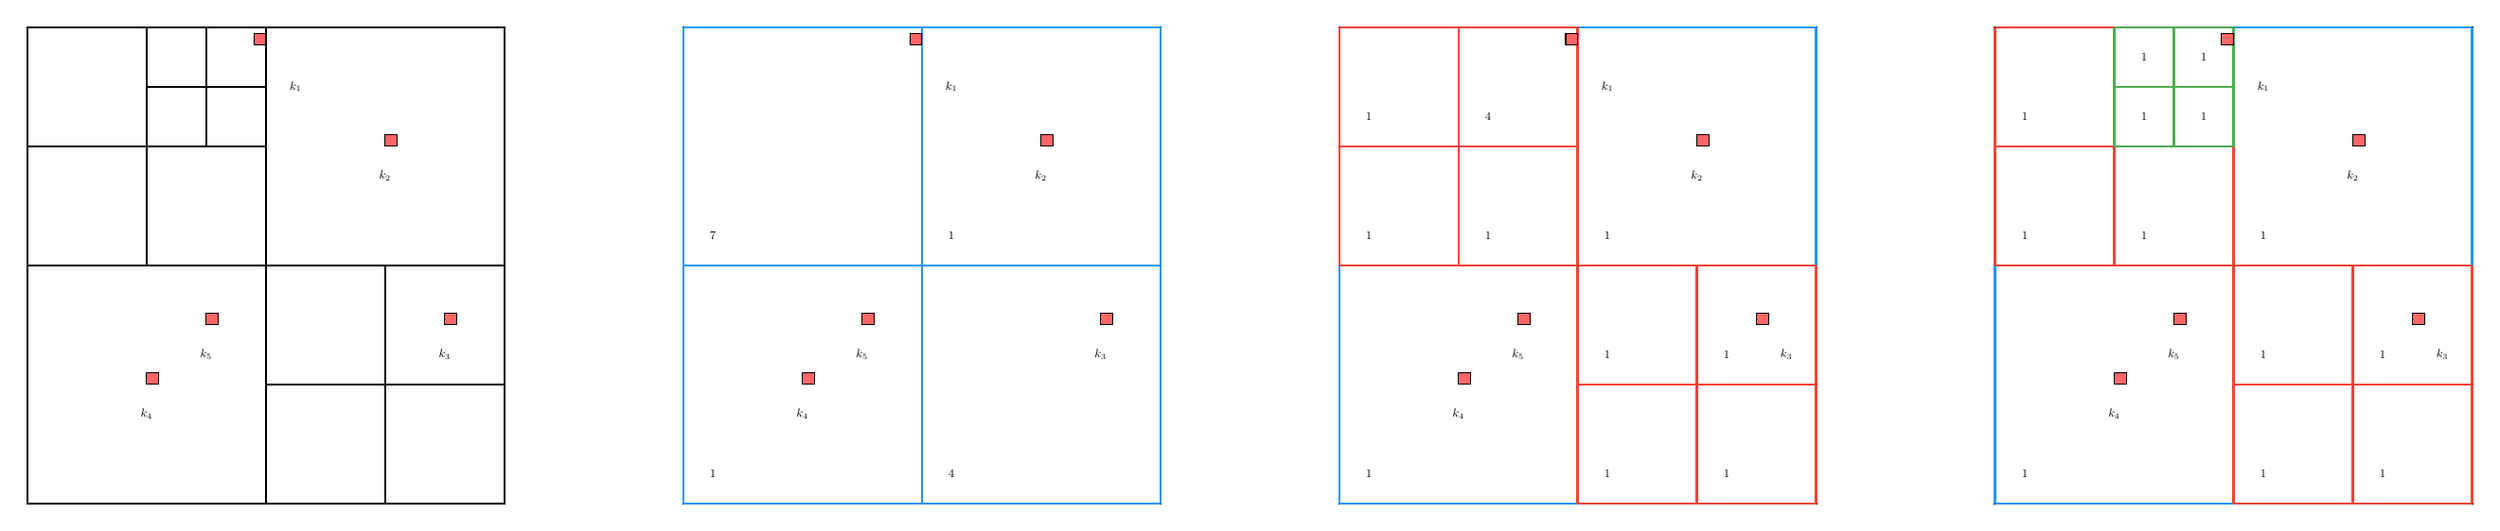
\begin{tikzpicture}[scale=0.8, every node/.style={scale=0.5}]
		
		% \draw[gray, very thin] (0,0) grid +(8,8);
		
		
		\begin{scope}[shift={(0,0)}]
		\draw[thick] (0,0) rectangle +(8,8);
		\draw[step=4,thick] (0,0) grid +(8,8);
		\draw[step=2,thick] (0,4) grid +(4,4);
		\draw[step=2,thick] (4,0) grid +(4,4);
		\draw[step=1,thick] (2,6) grid +(2,2);
		
		\draw[fill=red!60] (3.8,7.7) rectangle +(0.2,0.2);
		\node at (4.5,7.0) {\small $k_1$};
		\draw[fill=red!60] (6,6) rectangle +(0.2,0.2);
		\node at (6,5.5) {\small $k_2$};
		\draw[fill=red!60] (7,3) rectangle +(0.2,0.2);
		\node at (7,2.5) {\small $k_3$};
		\draw[fill=red!60] (2,2) rectangle +(0.2,0.2);
		\node at (2.0,1.5) {\small $k_4$};
		\draw[fill=red!60] (3,3) rectangle +(0.2,0.2);
		\node at (3.0,2.5) {\small $k_5$};
		
		\end{scope}	 	
		
		\begin{scope}[shift={(11,0)}]
		\draw[thick] (0,0) rectangle +(8,8);
		\draw[step=4,cpu4,thick] (0,0) grid +(8,8);
		
		\node at (0.5,0.5) {\small $1$};
		\node at (4.5,0.5) {\small $4$};
		\node at (0.5,4.5) {\small $7$};
		\node at (4.5,4.5) {\small $1$};
		
		\draw[fill=red!60] (3.8,7.7) rectangle +(0.2,0.2);
		\node at (4.5,7.0) {\small $k_1$};
		\draw[fill=red!60] (6,6) rectangle +(0.2,0.2);
		\node at (6,5.5) {\small $k_2$};
		\draw[fill=red!60] (7,3) rectangle +(0.2,0.2);
		\node at (7,2.5) {\small $k_3$};
		\draw[fill=red!60] (2,2) rectangle +(0.2,0.2);
		\node at (2.0,1.5) {\small $k_4$};
		\draw[fill=red!60] (3,3) rectangle +(0.2,0.2);
		\node at (3.0,2.5) {\small $k_5$};
		
		\end{scope}
		
		\begin{scope}[shift={(22,0)}]
		\draw[thick] (0,0) rectangle +(8,8);
		\draw[step=4,cpu4,thick] (0,0) grid +(8,8);
		\draw[step=2,cpu3,thick] (0,4) grid +(4,4);
		\draw[step=2,cpu3,thick] (4,0) grid +(4,4);
		\node at (0.5,0.5) {\small $1$};
		
		\node at (4.5,0.5) {\small $1$};
		\node at (6.5,0.5) {\small $1$};
		\node at (4.5,2.5) {\small $1$};
		\node at (6.5,2.5) {\small $1$};
		
		\node at (0.5,4.5) {\small $1$};
		\node at (2.5,4.5) {\small $1$};
		\node at (0.5,6.5) {\small $1$};
		\node at (2.5,6.5) {\small $4$};
		
		\node at (4.5,4.5) {\small $1$};	
		
		\draw[fill=red!60] (3.8,7.7) rectangle +(0.2,0.2);
		\node at (4.5,7.0) {\small $k_1$};
		\draw[fill=red!60] (6,6) rectangle +(0.2,0.2);
		\node at (6,5.5) {\small $k_2$};
		\draw[fill=red!60] (7,3) rectangle +(0.2,0.2);
		\node at (7.5,2.5) {\small $k_3$};
		\draw[fill=red!60] (2,2) rectangle +(0.2,0.2);
		\node at (2.0,1.5) {\small $k_4$};
		\draw[fill=red!60] (3,3) rectangle +(0.2,0.2);
		\node at (3.0,2.5) {\small $k_5$};
		\end{scope}
		
		\begin{scope}[shift={(33,0)}]
		\draw[thick] (0,0) rectangle +(8,8);
		\draw[step=4,cpu4,thick] (0,0) grid +(8,8);
		\draw[step=2,cpu3,thick] (0,4) grid +(4,4);
		\draw[step=2,cpu3,thick] (4,0) grid +(4,4);
		\draw[step=1,cpu1,thick] (2,6) grid +(2,2);
		
		\node at (0.5,0.5) {\small $1$};
		
		\node at (4.5,0.5) {\small $1$};
		\node at (6.5,0.5) {\small $1$};
		\node at (4.5,2.5) {\small $1$};
		\node at (6.5,2.5) {\small $1$};
		
		\node at (0.5,4.5) {\small $1$};
		\node at (2.5,4.5) {\small $1$};
		\node at (0.5,6.5) {\small $1$};
		
		\node at (2.5,6.5) {\small $1$};
		\node at (3.5,6.5) {\small $1$};
		\node at (2.5,7.5) {\small $1$};
		\node at (3.5,7.5) {\small $1$};
		
		\node at (4.5,4.5) {\small $1$};		
		
		
		\draw[fill=red!60] (3.8,7.7) rectangle +(0.2,0.2);
		\node at (4.5,7.0) {\small $k_1$};
		\draw[fill=red!60] (6,6) rectangle +(0.2,0.2);
		\node at (6,5.5) {\small $k_2$};
		\draw[fill=red!60] (7,3) rectangle +(0.2,0.2);
		\node at (7.5,2.5) {\small $k_3$};
		\draw[fill=red!60] (2,2) rectangle +(0.2,0.2);
		\node at (2.0,1.5) {\small $k_4$};
		\draw[fill=red!60] (3,3) rectangle +(0.2,0.2);
		\node at (3.0,2.5) {\small $k_5$};
		
		\end{scope}
		\end{tikzpicture}
	}
	\caption{\label{fig:sfcSearch}\small
		 %For a given ordered octree $\tau$  and a set of keys (leftmost figure),
		  \tsearch~ performs the traversal in a top-down order over the set of keys, while flagging $k_2,k_4,k_5$ at the level $1$ split, $k_3$ at level $2$ split, and $k_1$ at level $3$ split. %Note that numbers inside the octants (i.e. bucket count) represent the number of octants in $\tau$ belongs to that bucket at splitting level $l$. When bucket count of octant $e\in \tau$ reaches $1$, all the keys in that bucket flagged as found and $e$ is considered to be the search result for those keys. 
	}
	\vspace{-0.15in}
\end{figure}
\end{textblock}

\begin{textblock}{8}(0,8.4)
\begin{figure}
	\centering
	\begin{tikzpicture}
	\begin{axis}[legend pos= north west,xlabel={number of keys $\rightarrow$},symbolic x coords={100,1K,10K,100K,1M,10M,20M,33M,64M},
	xtick={data},
	ylabel={time(s) $\rightarrow$},grid=major,width=6in,height=3in,
	x tick label style={font=\tiny}]
	\addplot [sq_b1,thin,mark=*]table [x={numKeys},y={bsearch_time_s}]{dat/stampede2/tsearch.dat};
	\addplot [sq_r1,thin,mark=x] table [x={numKeys},y={tsearch_time_s}]{dat/stampede2/tsearch.dat};
	\legend{\texttt{std::bsearch}, \tsearch }
	\end{axis}
	\end{tikzpicture}
	\caption{Comparison of \texttt{std::bsearch} with operator $<$ and comparison free \tsearch~ approach for performing, varying number of keys on $33M$ sorted octree in \Stampede~ \texttt{SKX} node.}
	\label{fig::balcomparison}
\end{figure}
\end{textblock}

%\begin{textblock}{7}(7.5,0)
%\Subhead{\oTo: Octant to Octant map}
%\vspace{-0.5in}
%\captionof{algorithm}{\small \teToe: compute \oTo \label{alg:e2e}}
%	\small
%	\begin{algorithmic}[1]
%		\Require an ordered 2:1 balanced distributed octree $\mathcal{T}$ %on $\Gamma$, $\mathit{comm}$, $p$,
%%		$p_r$ of current task in $\mathit{comm}$.
%		\Ensure compute \oTo %$\phi_{\hat{\tau_k}}$
%		\State $\hat{\tau_{p_r}} \leftarrow \tghost(\mathcal{T},comm,p,p_r)$
%		\State \oTo $~\leftarrow \emptyset$ % $\phi_{\hat{\tau_{p_r}}}[]
%		\State $keys [] \leftarrow$ compute $\mathcal{K}(\hat{\tau_{pr}})$ 
%		\State $\tsearch(\hat{\tau_{p_r}},keys)$ 
%		\For {$key \in keys$}
%		\If {$key$ is found}
%		\State \oTo [key.owner][key.neighbor]=key.result
%		\EndIf
%		\EndFor
%		\State \Return \oTo
%	\end{algorithmic}
%\vspace{0.5in}
%\Subhead{\oTn: Octant to Nodal map}
%\vspace{-0.5in}
%\captionof{algorithm}{\small \teTon: Octant to nodal map generation - \oTn \label{alg:e2n}}
%	\small
%\begin{algorithmic}[1]
%		\Require an ordered 2:1 balanced distributed octree $\mathcal{T}$ %on $\Gamma$, $\mathit{comm}$, $p$,
%%		$p_r$ of current task in $\mathit{comm}$.
%		\Ensure compute \oTn % $\psi_{\hat{\tau_k}}$
%%		\State $\hat{\tau_{p_r}} \leftarrow \tghost(\mathcal{T},comm,p,p_r)$
%		%	\State $\mathcal{V}_L [] \leftarrow$ initialize()
%		\State \oTn $~ [] \leftarrow $ $initialize(\mathcal{V}_L)$ \Comment{ \oTn ~initialized with \dgn} 
%		%	\State $nodes\_duplicate [] \leftarrow $ compute $\rho(\mathcal{T})$ 
%		\State $\mathcal{V}_S \leftarrow $ $\mathcal{V}_L \setminus \mathcal{V}_D$
%		%	\State $nodes\_cg [] \leftarrow$ compute $\mathcal{V}_L(\mathcal{T})$
%		\For {$e\in \hat{\tau_k}$}
%		\For {$v\in N_d(e)$} \Comment{$N_d(e)$ denotes $(d+1)^3$ nodes of $e$} 
%		\State $owner\_idx\leftarrow $ compute $\mathcal{O}(v)$
%		\State \oTn $~ \leftarrow owner\_idx$
%		\EndFor
%		\EndFor 	
%		\State \Return \oTn
%\end{algorithmic}
%
%
%\end{textblock}

%\begin{textblock}{7}(7.5,0)
%\Subhead{Hanging nodes}	
%		\begin{figure}
%		\centering
%		\resizebox{!}{1.5\TPHorizModule}{
%			\begin{tikzpicture}[scale=0.32,>=stealth,bluearr/.style={->,blue,shorten >= 3pt}]
%			
%			\begin{scope}[shift={(0,0)}]
%			\drawcubeII(0,0,0,8,black,blue!50,0.3);
%			\drawcubeII(10,0,0,4,black,green!50,0.3);
%			\foreach \y in {0,2,...,4}
%			{
%				\foreach \z in {0,2,...,4}{
%					\draw[fill=red!60] (10,\y,\z) circle (0.12);
%					\draw[fill=red!80] (8,2*\y,2*\z) circle (0.15);
%					\draw[bluearr] (10,\y,\z) to [bend left=45] node [midway,above,anchor=east,align=center] {} (8,2*\y,2*\z);
%				}
%			}	
%			
%			\end{scope}
%			
%			\begin{scope}[shift={(18,0)}]
%			
%			\drawcubeII(0,0,0,8,black,blue!50,0.3);
%			\drawcubeII(10,0,-4,4,black,green!50,0.3);
%			\foreach \z in {0,2,...,4}{
%				\draw[fill=red!60] (10,\z,0) circle (0.12);
%				\draw[fill=red!80] (8,2*\z,0) circle (0.15);
%				\draw[bluearr] (10,\z,0) to [bend left=45] node [midway,above,anchor=east,align=center] {} (8,2*\z,0);
%			}
%			
%			%\drawcubeII(0,0,0,8,black,blue!50,0.3);
%			%\drawcubeII(10,10,0,4,black,green!50,0.3);
%			%\foreach \z in {0,2,...,4}{
%			%	\draw[fill=red!60] (10,10,\z) circle (0.12);
%			%	\draw[fill=red!80] (8,8,2*\z) circle (0.15);
%			%	\draw[bluearr] (10,10,\z) to [out=120,in=180] node [midway,above,anchor=east,align=center] {} (8,8,2*\z);
%			%}
%			
%			
%			\end{scope}
%			
%			\end{tikzpicture}}
%		\caption{\small An example of a hanging face  and a hanging edge where in both cases octant (\textcolor{green!50}{$\blacksquare$})  has a hanging face (left figure) and  a hanging edge (right figure) with octant (\textcolor{blue!50}{$\blacksquare$}). Nodes on the hanging face/edge are mapped to the larger octant and the hanging nodal values are obtained via interpolation. 
%			Note that for illustrative purposes, the two octants are drawn separately, but are contiguous.\label{fig:hangingElementsNodes} }
%		\vspace{-0.15in}
%	\end{figure}
%	
%	\vspace{0.5in}
%\Subhead{\cgn~ \& \dgn}		
%	\begin{figure}
%		\centering
%		\resizebox{!}{1.5\TPHorizModule}{
%			\begin{tikzpicture}[scale=0.2,every node/.style={scale=0.6}]
%			
%			\begin{scope}[shift={(0,0)}]
%			\draw[step=5] (0,0) grid +(10,10);
%			\draw[step=2.5] (5,0) grid +(5,5);
%			\draw[step=2.5] (0,5) grid +(5,5);
%			
%			%\draw[fill=red!60] (4.2,4.2) circle (0.15);
%			\end{scope}
%			
%			\begin{scope}[shift={(15,0)}]
%			\draw[step=5] (0,0) grid +(10,10);
%			\draw[step=2.5] (5,0) grid +(5,5);
%			\draw[step=2.5] (0,5) grid +(5,5);
%			
%			\def \r{0.1}
%			\foreach \x in {0.2,2.5,4.8}{
%				\foreach \y in {0.2,2.5,4.8}{
%					\draw[red,fill=red] (\x,\y) circle (\r);
%				}
%			}
%			
%			\foreach \x in {5.2,7.5,9.8}{
%				\foreach \y in {5.2,7.5,9.8}{
%					\draw[red,fill=red] (\x,\y) circle (\r);
%				}
%			}	
%			
%			\foreach \x in {0.2,1.25,2.3,2.7,3.75,4.8}{
%				\foreach \y in {5.2,6.25,7.3}{
%					\draw[blue,fill=blue] (\x,\y) circle (\r);
%				}
%				\foreach \y in {7.7,8.75,9.8}{
%					\draw[blue,fill=blue] (\x,\y) circle (\r);
%				}  
%			}
%			
%			\foreach \x in {5.2,6.25,7.3,7.7,8.75,9.8}{
%				\foreach \y in {0.2,1.25,2.3}{
%					\draw[blue,fill=blue] (\x,\y) circle (\r);
%				}
%				\foreach \y in {2.7,3.75,4.8}{
%					\draw[blue,fill=blue] (\x,\y) circle (\r);
%				}  
%			}
%			
%			\end{scope}
%			
%			\begin{scope}[shift={(33,0)}]
%			
%			\draw[step=5] (0,0) grid +(10,10);
%			\draw[step=2.5] (5,0) grid +(5,5);
%			\draw[step=2.5] (0,5) grid +(5,5);
%			
%			\def \r{0.12}
%			\foreach \x in {0,2.5,5}{
%				\foreach \y in {0,2.5,5}{
%					\draw[red,fill=red] (\x,\y) circle (\r);
%				}
%			}
%			
%			\foreach \x in {5,7.5,10}{
%				\foreach \y in {5,7.5,10}{
%					\draw[red,fill=red] (\x,\y) circle (\r);
%				}
%			}
%			
%			\foreach \x in {0,1.25,2.5,3.75}{
%				\foreach \y in {6.25,7.5,8.75,10}{
%					\draw[blue,fill=blue] (\x,\y) circle (\r);
%				}
%			}	
%			
%			\foreach \x in {6.25,7.5,8.75,10}{
%				\foreach \y in {0,1.25,2.5,3.75}{
%					\draw[blue,fill=blue] (\x,\y) circle (\r);
%				}
%			}
%			
%			\end{scope}	
%			\end{tikzpicture}
%		}
%		\caption{\label{fig:dg_to_cg} \small A $2D$ example of \dgn~ (in the center) and \cgn~(the rightmost figure) nodal representation (for octant order of $2$) of the adaptive quadtree shown in the leftmost figure. Note that in \dgn~ representation nodes are local to each octant and contain duplicate nodes. By removing all the duplicate and hanging nodes by the rule of nodal ownership we get the \cgn~ representation. Note that the nodes are color coded based on the octant level.}
%		\vspace{-0.15in}
%	\end{figure}
%\end{textblock}

% mesh end textblock
\end{textblock}



\begin{textblock}{8}(9,11.5)
\Subhead{Zip \& Unzip: FD computations on adaptive octrees}\\
\textbf{Unzip} : process of generating regular grid blocks from adaptive octree with required padding region for stencil computations.  \\
\textbf{Zip} : inverse process of unzip to \cgn~ representation. \\
\textbf{Note}: All the communication happens in the \textit{zip} states since \textit{unzip} contains duplicate nodes. 
%\vspace{0.3in}
\begin{figure}
	\centering
	\resizebox{!}{4.8\TPHorizModule}{
		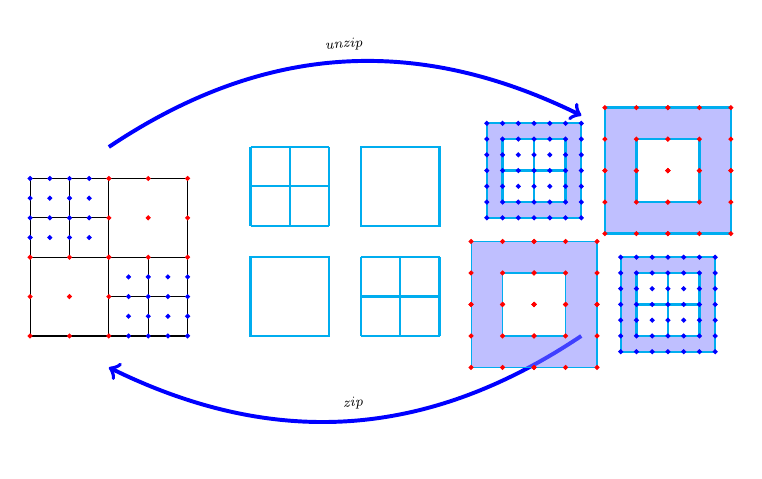
\begin{tikzpicture}[scale=0.2,every node/.style={scale=0.6}]
		\path [blue,fill=cyan,line width=0.5mm,bend left,->,every node/.style={black,sloped,anchor=south,auto=false}] (5,12) edge node{\textit{\ \tiny unzip}} (35,14);
		\path [blue,fill=cyan,line width=0.5mm,bend left,->,every node/.style={black,sloped,anchor=south,auto=false}] (35,0) edge node{\textit{\ \tiny zip}} (5,-2);
		\begin{scope}[shift={(0,0)}]
		\draw[step=5cm] (0,0) grid +(10,10);
		\draw[step=2.5cm] (5,0) grid +(5,5);
		\draw[step=2.5cm] (0,5) grid +(5,5);
		
		\def \r{0.12}
		\foreach \x in {0,2.5,5}{
			\foreach \y in {0,2.5,5}{
				\draw[red,fill=red] (\x,\y) circle (\r);
			}
		}
		
		\foreach \x in {5,7.5,10}{
			\foreach \y in {5,7.5,10}{
				\draw[red,fill=red] (\x,\y) circle (\r);
			}
		}
		
		\foreach \x in {0,1.25,2.5,3.75}{
			\foreach \y in {6.25,7.5,8.75,10}{
				\draw[blue,fill=blue] (\x,\y) circle (\r);
			}
		}	
		
		\foreach \x in {6.25,7.5,8.75,10}{
			\foreach \y in {0,1.25,2.5,3.75}{
				\draw[blue,fill=blue] (\x,\y) circle (\r);
			}
		}
		\end{scope}
		
		\begin{scope}[shift={(14,0)}]
		%\draw[cyan,thick,fill=blue!20] (-1,-1) rectangle +(6,6);
		\draw[cyan,thick] (0,0) rectangle +(5,5);
		\draw[cyan,thick,xshift=2cm,yshift=2.0cm] (5,5) rectangle +(5,5);
		\draw[cyan,thick,step=2.5cm,xshift=2.0cm] (5,0) grid +(5,5);
		\draw[cyan,thick,step=2.5cm,yshift=2.0cm] (0,5) grid +(5,5);
		%	\draw[cyan,thick] (0,4) rectangle +(2,2);
		%	\draw[cyan,thick] (2,4) rectangle +(2,2);
		%	\draw[cyan,thick] (2,6) rectangle +(2,2);
		%	\draw[cyan,thick] (4,0) rectangle +(2,2);
		%	\draw[cyan,thick] (6,2) rectangle +(2,2);
		%	\draw[cyan,thick] (6,0) rectangle +(2,2);
		\end{scope}
		
		\begin{scope}[shift={(30,0)}]
		\def \r{0.12}
		\draw[cyan,fill=blue!50,fill opacity=0.5]
		(-2,-2)--(-2,6)--(6,6)--(6,-2)--cycle
		(0,0) -- (4,0)-- (4,4)--(0,4)--cycle;
		\foreach \x in {-2,0,2,2,4,6}{
			\foreach \y in {-2,0,2,2,4,6}{
				\draw[red,fill=red] (\x,\y) circle (\r);
			}
		}
		
		\draw[cyan,thick,fill=blue!50,fill opacity=0.5,even odd rule,xshift=8.5cm,yshift=8.5cm] 
		(-2,-2)--(-2,6)--(6,6)--(6,-2)--cycle
		(0,0) -- (4,0)-- (4,4)--(0,4)--cycle;
		\foreach \x in {-2,0,2,2,4,6}{
			\foreach \y in {-2,0,2,2,4,6}{
				\draw[red,fill=red,xshift=8.5cm,yshift=8.5cm] (\x,\y) circle (\r);
			}
		}
		
		\draw[cyan,thick,fill=blue!50,fill opacity=0.5,even odd rule,xshift=8.5cm] 
		(-1,-1)--(-1,5)--(5,5)--(5,-1)--cycle
		(0,0) -- (4,0)-- (4,4)--(0,4)--cycle;
		\draw[cyan,thick,step=2,xshift=8.5cm] (0,0) grid +(4,4);
		\foreach \x in {-1,0,1,2,3,4,5}{
			\foreach \y in {-1,0,1,2,3,4,5}{
				\draw[blue,fill=blue,xshift=8.5cm] (\x,\y) circle (\r);
			}
		}
		
		\draw[cyan,thick,fill=blue!50,fill opacity=0.5,even odd rule,yshift=8.5cm] 
		(-1,-1)--(-1,5)--(5,5)--(5,-1)--cycle
		(0,0) -- (4,0)-- (4,4)--(0,4)--cycle;
		\draw[cyan,thick,step=2,yshift=8.5cm] (0,0) grid +(4,4);	
		\foreach \x in {-1,0,1,2,3,4,5}{
			\foreach \y in {-1,0,1,2,3,4,5}{
				\draw[blue,fill=blue,yshift=8.5cm] (\x,\y) circle (\r);
			}
		}
		
		\end{scope}	
		\end{tikzpicture}
	}	
	\caption{\label{fig:unzip} A simplistic example of octree to block decomposition and \unzip~ operation. The leftmost figure shows the considering adaptive octree with \cgn~ and its block decomposition is shown in the middle. Note that the given octree is decomposed into four regular blocks of different sizes. The rightmost figure shows the decomposed blocks padded with values coming from neighboring octants with interpolation if needed. In order to perform \unzip~ operation both $\psi$ and $\psi$ mappings are used. }
	\vspace{-0.15in}
\end{figure}

\end{textblock}

\begin{textblock}{14}(18,12.5)
	\Subhead{Simple example: Non-linear sigma model}
	
		\begin{figure}
%		\noindent\fbox{
			\begin{minipage}[t]{.48\textwidth}
%				\small
				\begin{eqnarray*}
				\partial_t\phi &=& \Delta \chi -\frac{\sin(2\chi)}{{\norm{x}_2}^2} \\
				\partial_t\chi &=& \phi 
				\end{eqnarray*}
			\end{minipage}% This must go next to `\end{minipage}`
%		}
		\begin{minipage}[t]{.5\textwidth}
			\small
%frame=single,framesep=2pt,
\begin{minted}[frame=single,framesep=1pt,bgcolor=yellow!10]{python}
 from DENDRO_sym import *
 phi_rhs = sum(d2(i,i,chi)for i in dendro.e_i) 
 		- sin(2*chi)/r**2
 chi_rhs = phi
\end{minted}
		\end{minipage}
		%\caption{\label{fig:symb} \small The left panel shows the \BSSN ~formulation of the Einstein equations. These are tensor equations, with indices $i,j,\ldots$ taking the values $1, 2, 3$. On the right we show the \texttt{{\dendro\_sym}} code for these equations. \texttt{\dendro\_sym} uses \texttt{SymPy} and other tools to generate optimized C++ code to evaluate the equations. Note that $\mathcal{L}_\beta,\ D,\ \partial$ denote Lie derivative, covariant derivative and partial derivative respectively, and we have excluded $\partial_t\Gamma^i$ from \texttt{\dendro\_sym} to save space.}
		%\label{fig:bssneqs}
		\vspace{-0.15in}
	\end{figure}
	\vspace{0.7in}
	
	\begin{figure}
		\begin{subfigure}{0.33\textwidth}
			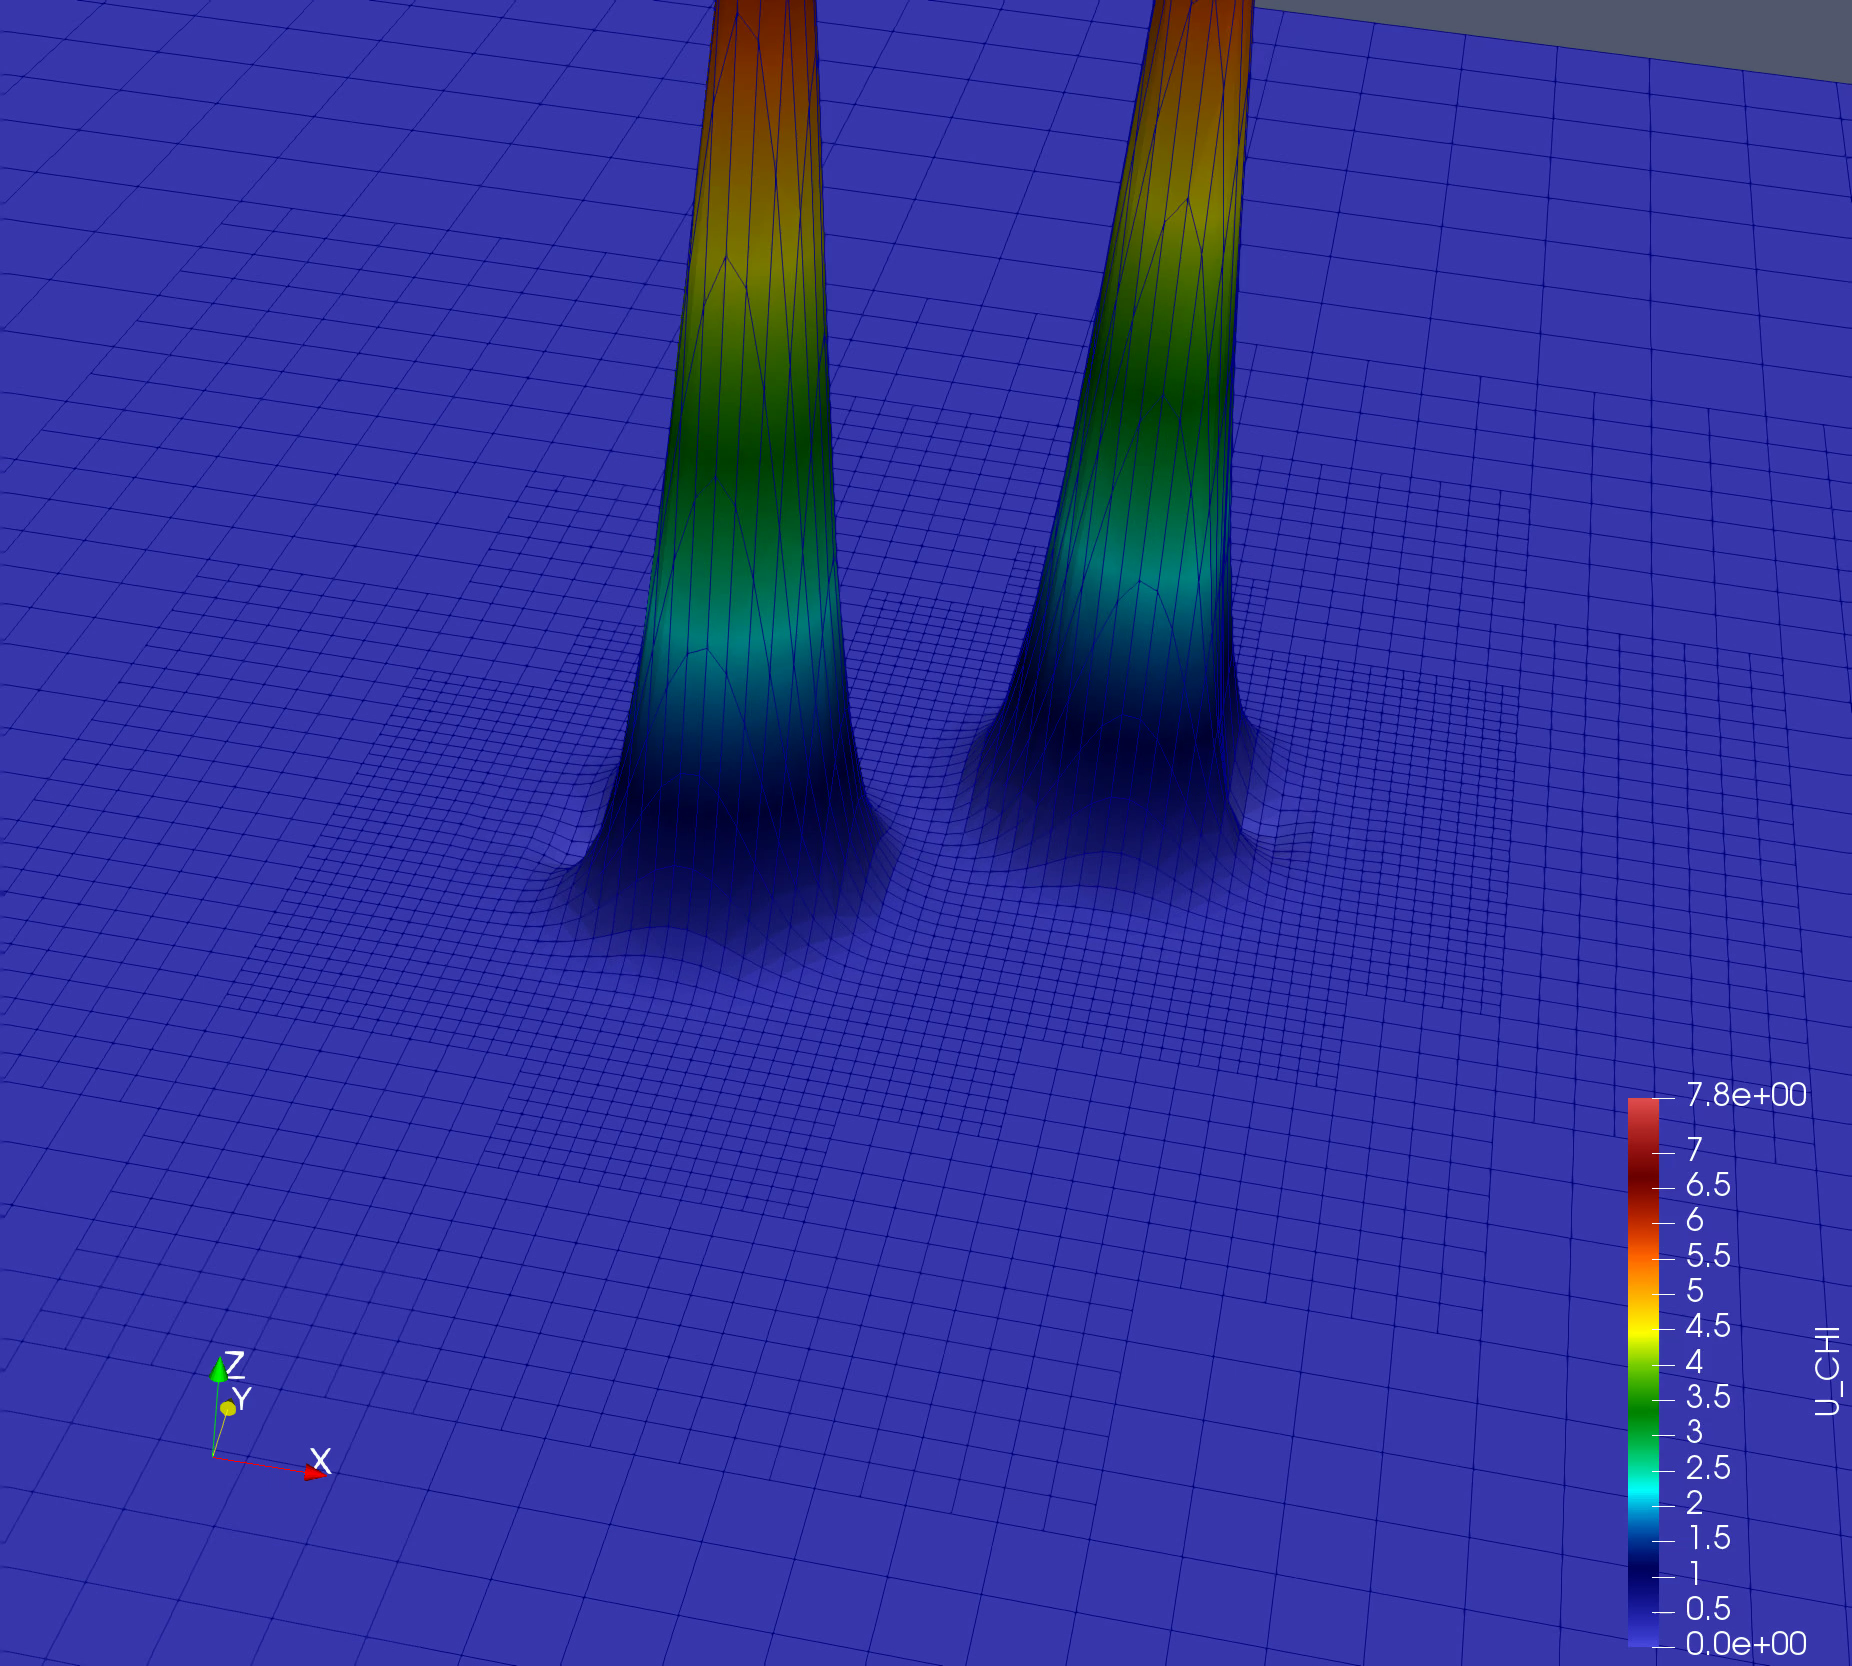
\includegraphics[width=0.9\textwidth]{figs/nlsmB0.png}
			\caption{step=0}			
		\end{subfigure}
		\begin{subfigure}{0.33\textwidth}
			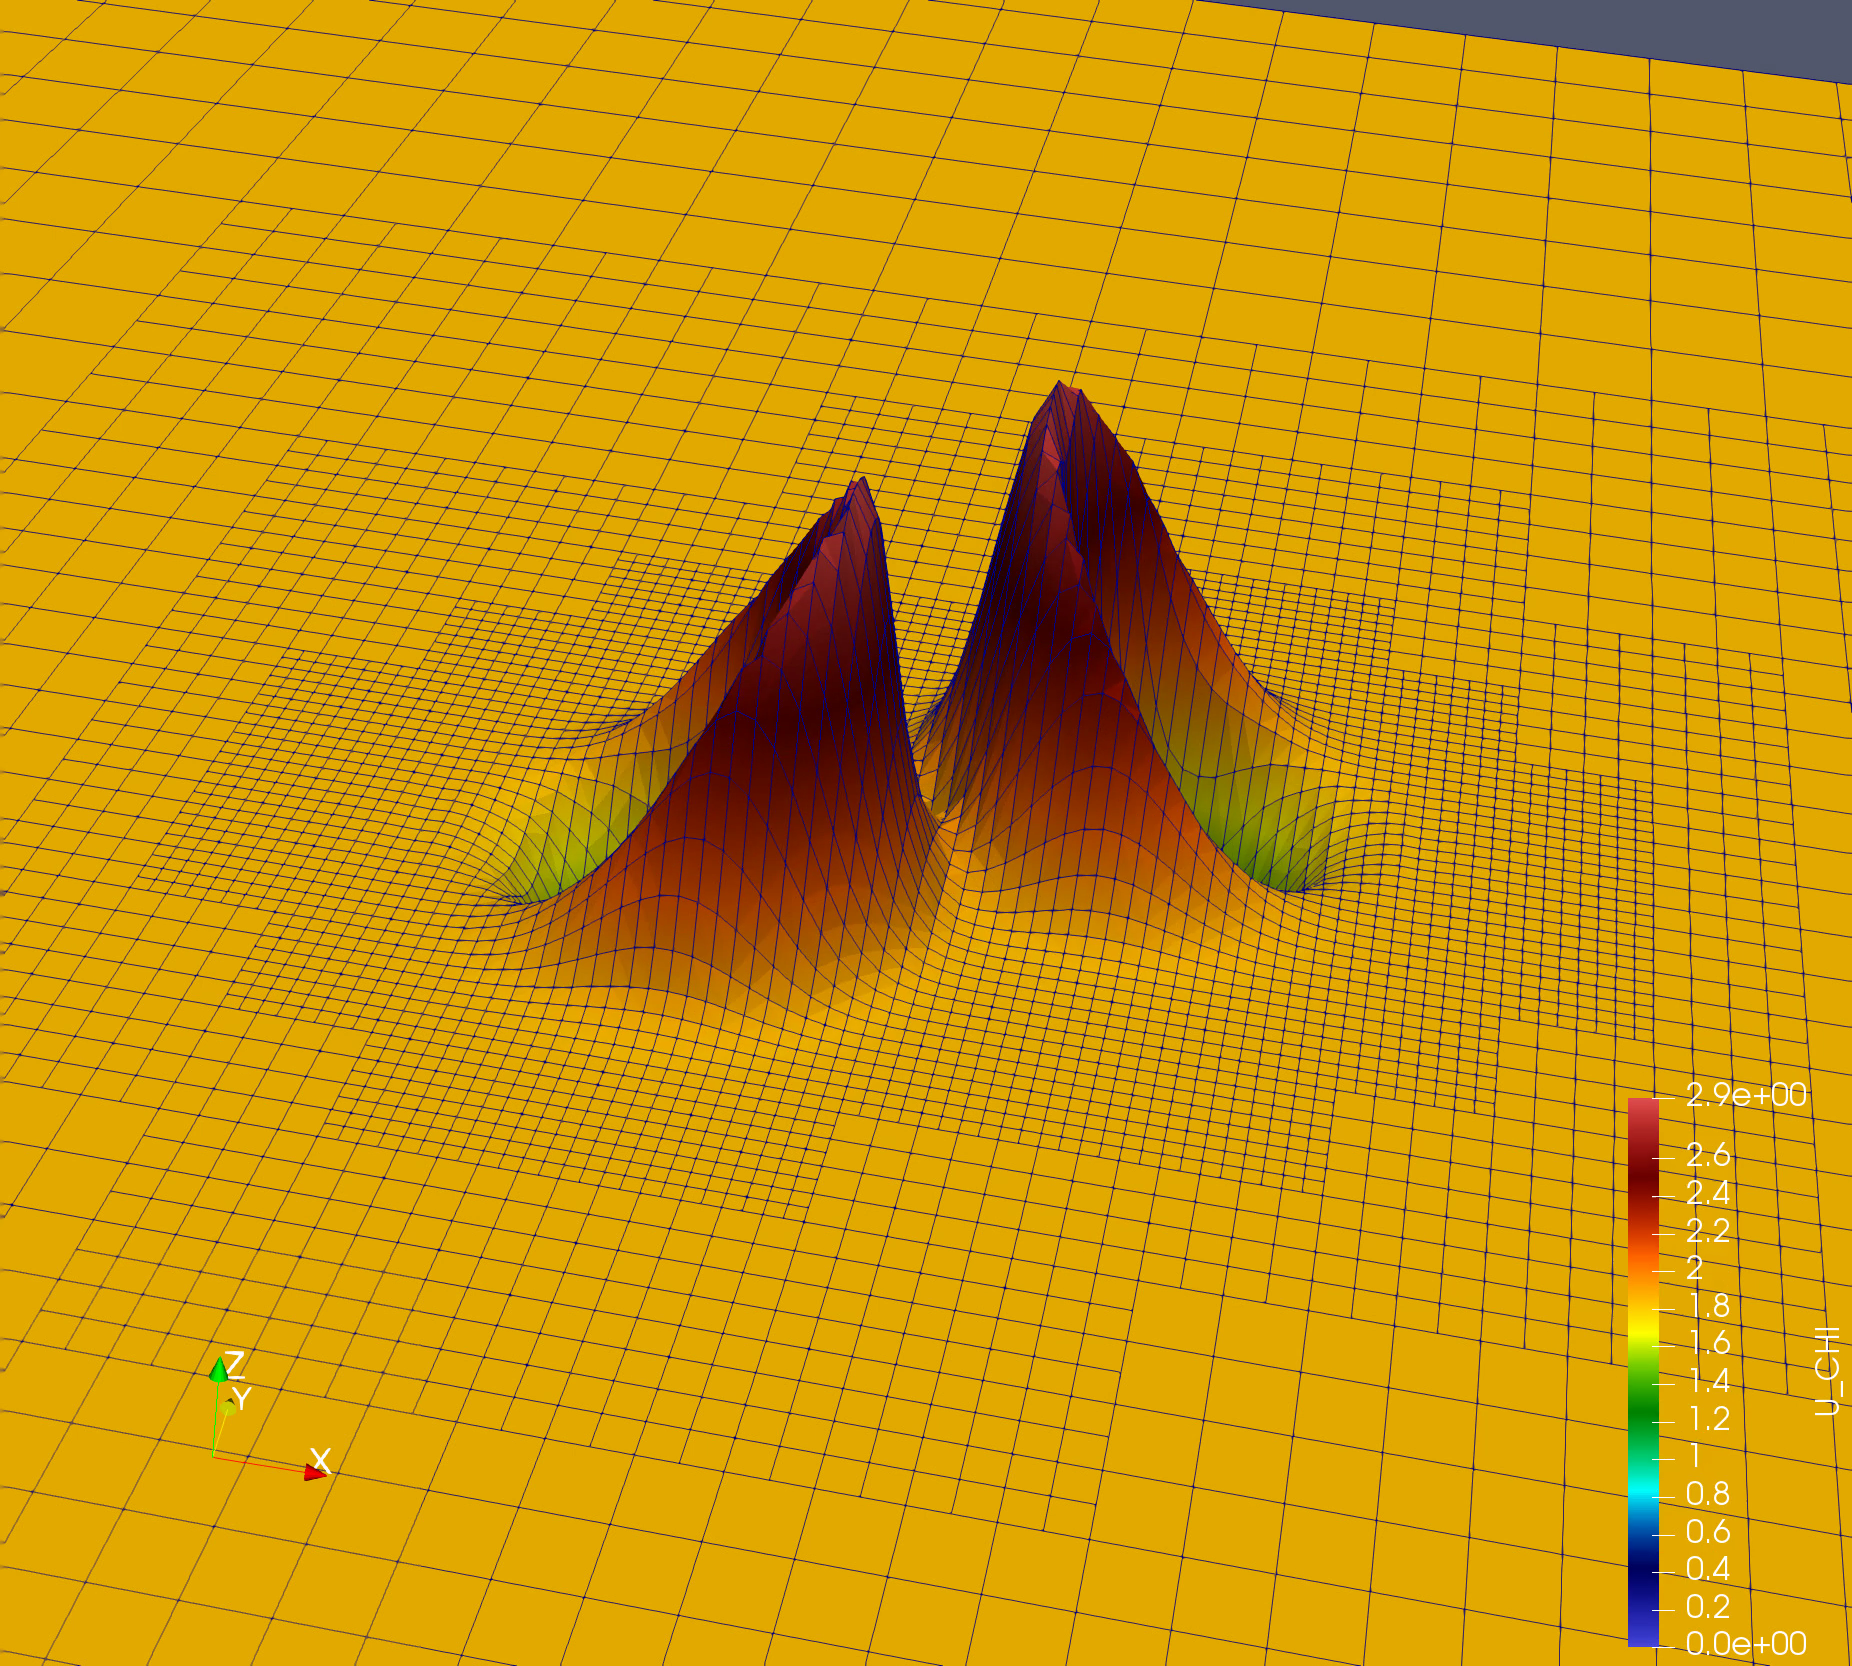
\includegraphics[width=0.9\textwidth]{figs/nlsmB7.png}
			\caption{step=7}			
		\end{subfigure}
		\begin{subfigure}{0.33\textwidth}
			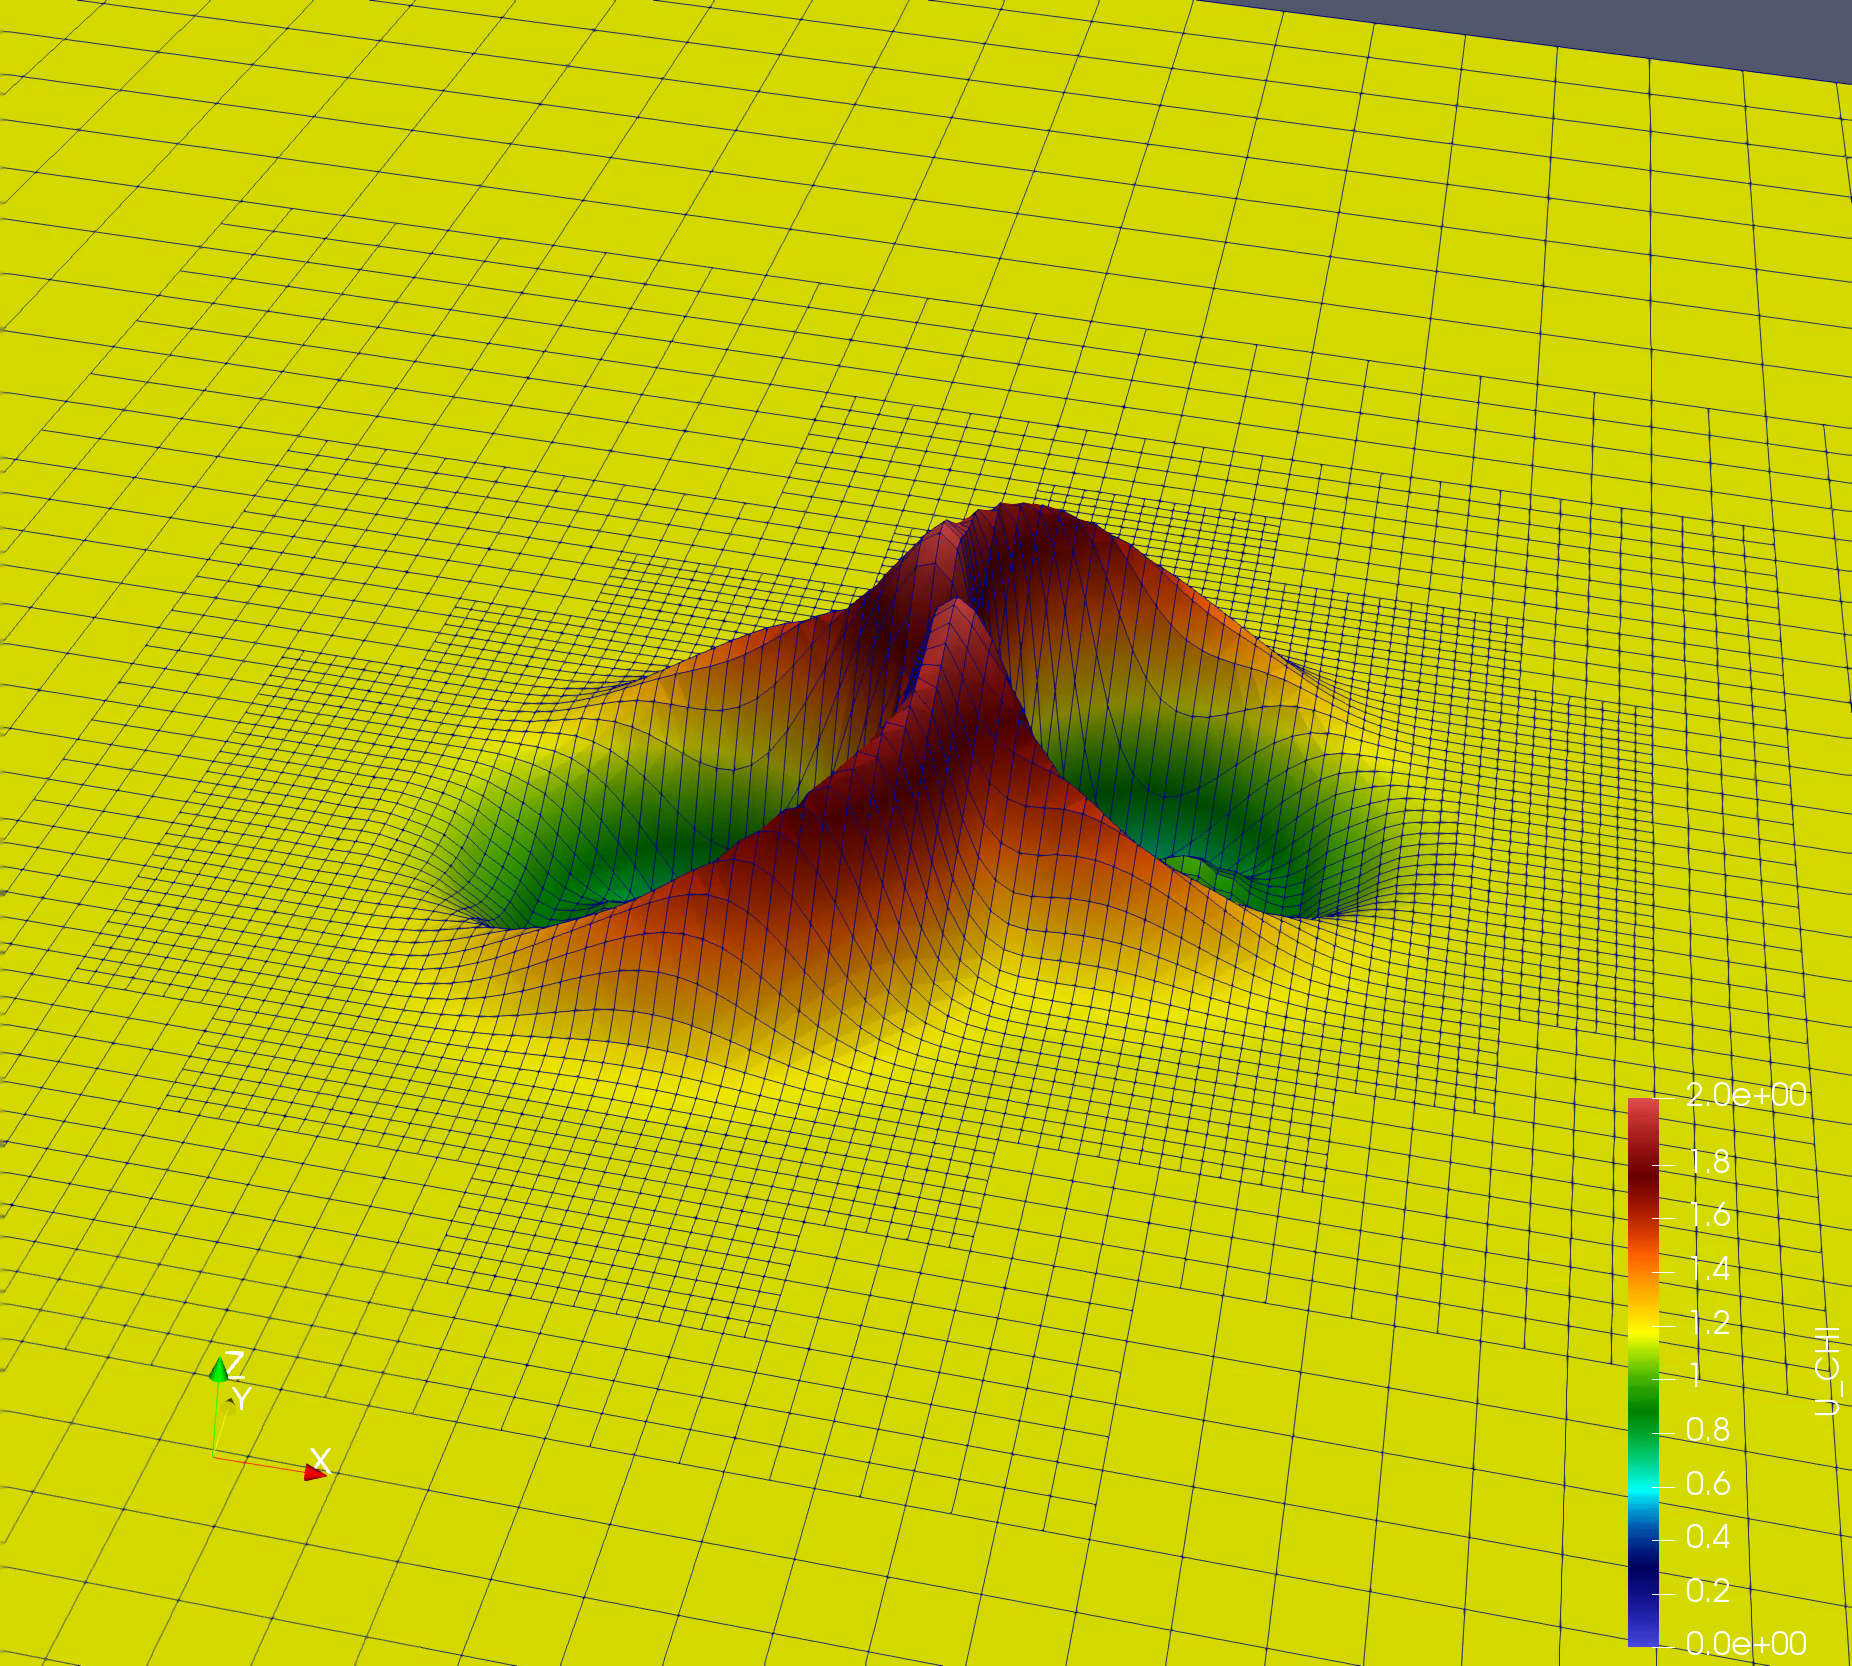
\includegraphics[width=0.9\textwidth]{figs/nlsmB11.png}
			\caption{step=11}
		\end{subfigure}\hfil
		\begin{subfigure}{0.33\textwidth}
			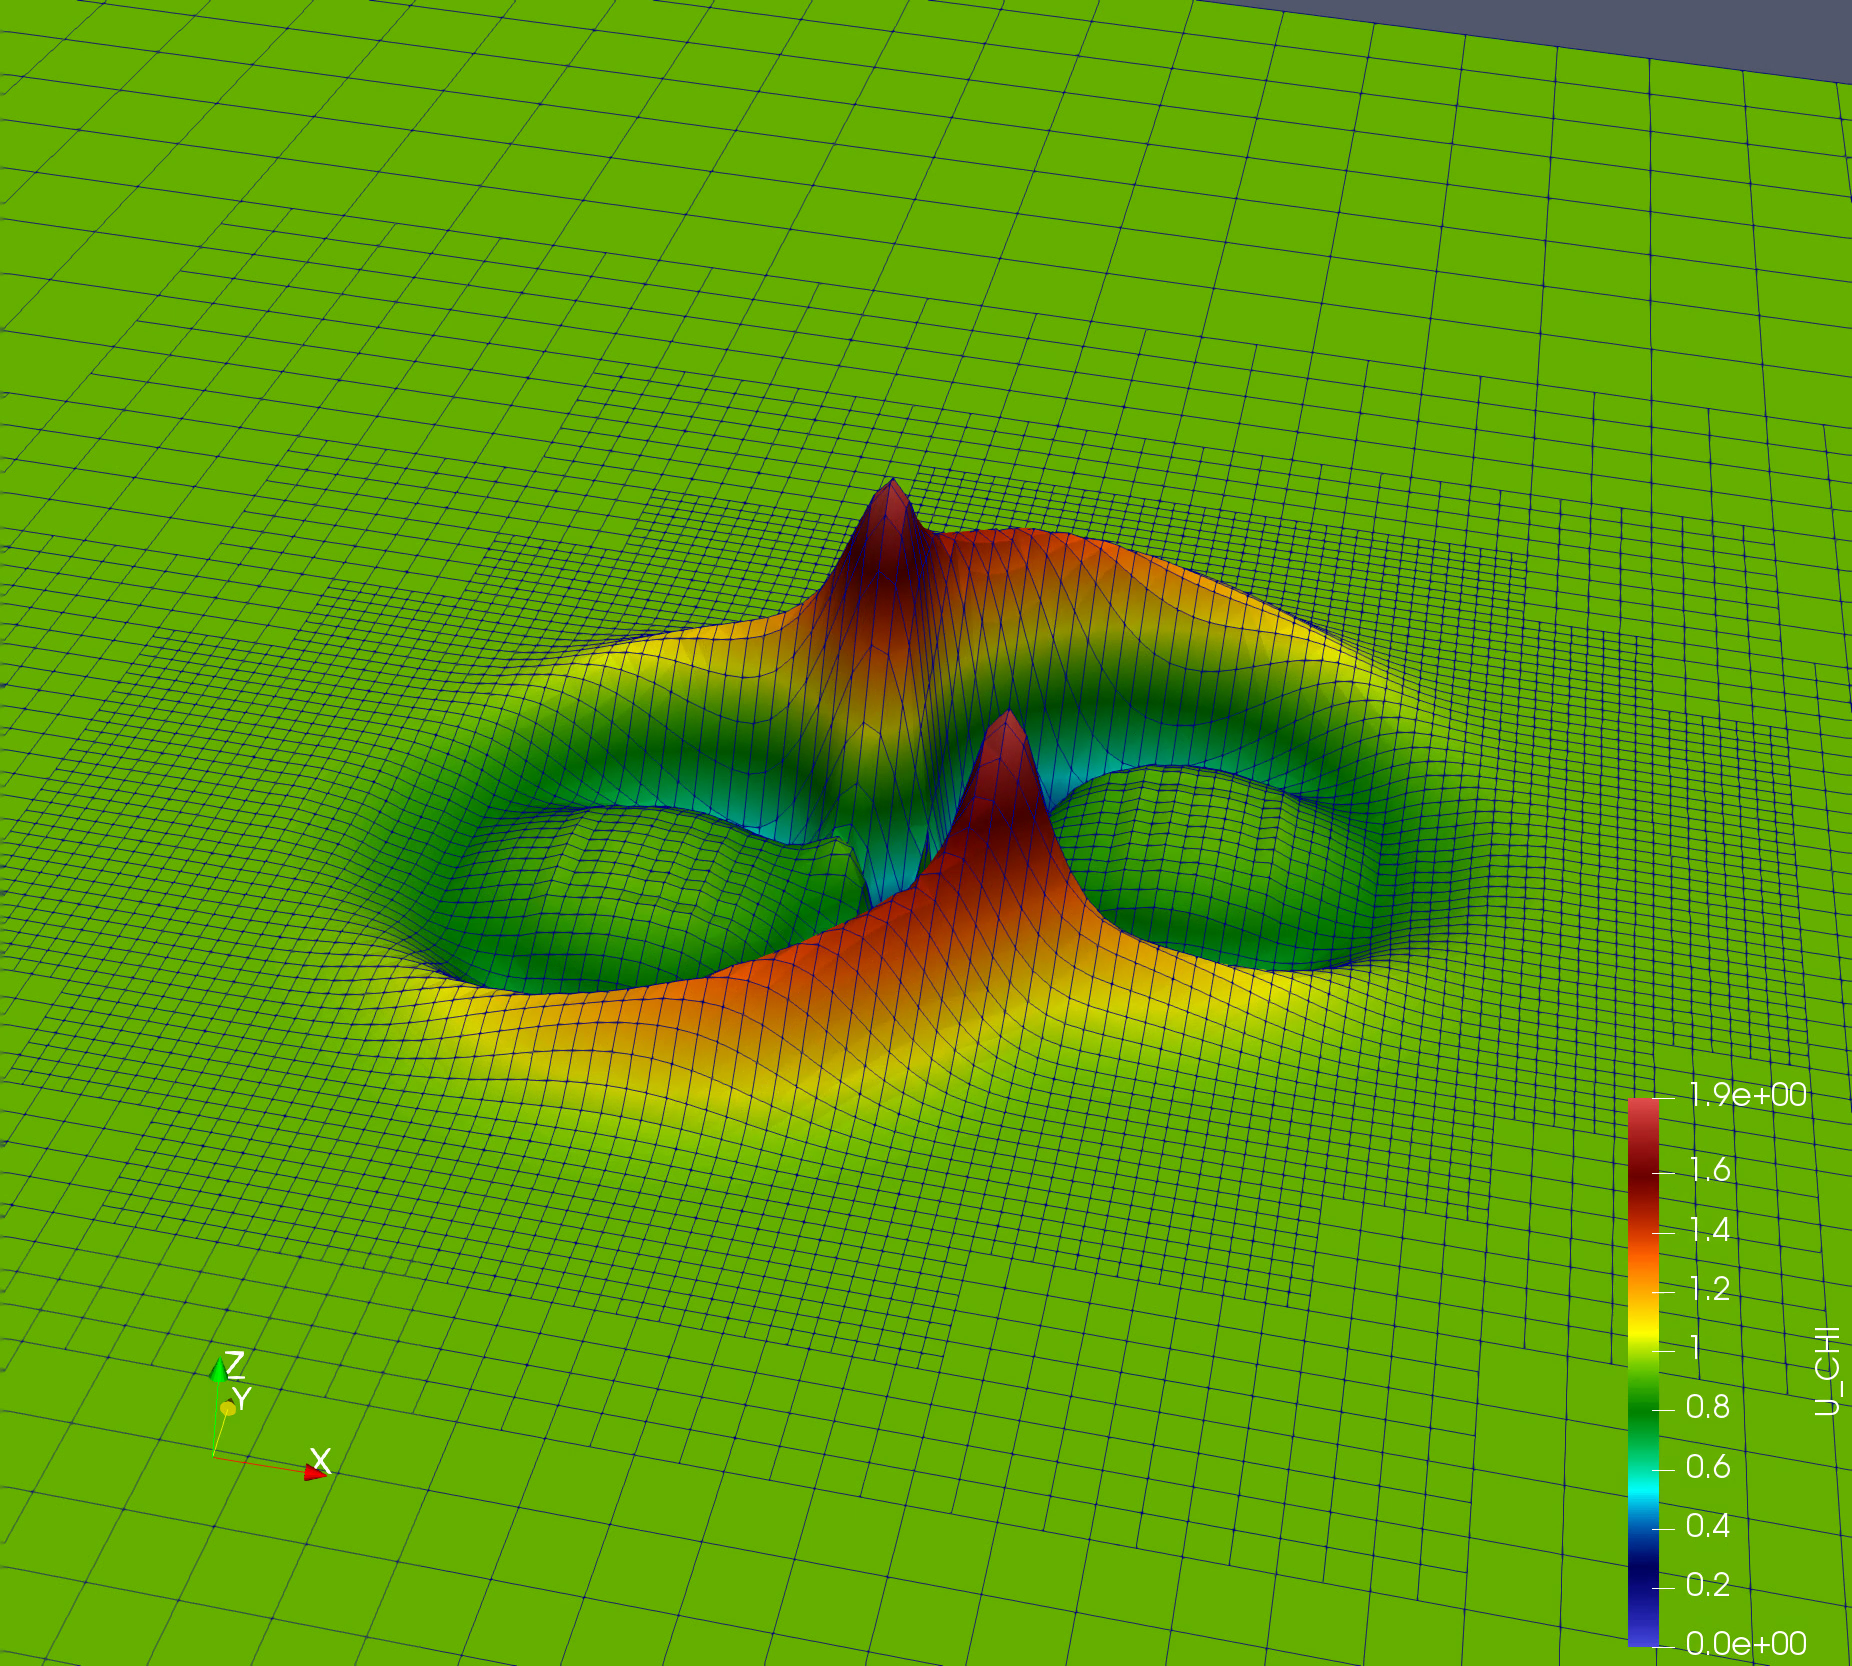
\includegraphics[width=0.9\textwidth]{figs/nlsmB16.png}
			\caption{step=16}			
		\end{subfigure}
		\begin{subfigure}{0.33\textwidth}
			\includegraphics[width=0.9\textwidth]{figs/nlsmB23.png}
			\caption{step=23}
		\end{subfigure}
		\begin{subfigure}{0.33\textwidth}
			\includegraphics[width=0.9\textwidth]{figs/nlsmB44.png}
			\caption{step=44}
		\end{subfigure}
		\caption{Time step snapshots of a $z$ plane slice of $3D$ \NLSM~ with two initial Gaussian distributions with Runge-Kutta time stepping scheme. Note that how the mesh refines (based on the WAMR) as the waves 
			propagate away from the origin.   \label{fig:nlsmB}}
		\vspace{-0.2in}
	\end{figure}
	
\end{textblock}


\end{textblock}




%%%%%%===== Results==============================


\begin{textblock}{25}(53,5)
{\color{DarkBlue}\hrule}\medskip
\Head{Results}

\begin{textblock}{24}(0,12.5)
%\Subhead{Comparison with Einstein Toolkit (ET) }
\vspace{-0.2in}
\begin{figure}
	\centering
	\resizebox{24\TPHorizModule}{!}{
	\begin{tikzpicture}[scale=1.0,every node/.style={scale=0.65}]
	\begin{axis}[
	ylabel={time per $RK$ step (s) $\rightarrow$},
	% xlabel={number of cores $\rightarrow$},
	legend pos=north west,symbolic x coords={48,96,192,384,768,1536,3072},xtick = data,
	height=3.38in,
	width=3.38in,
	%extra x tick style={tick label style={black, below, yshift=1.5ex}},
	xticklabels=\empty,
	ticklabel style={left}, grid=major, 
	extra x ticks={48,96,192,384,768,1536,3072},
	extra x tick labels={48,96,192,384,768,1536,3072},
	extra x tick style={tick label style={black, below, yshift=-0.7ex,font=\small,rotate=45}},
	legend style={at={(0.6,1.05)},anchor=south},
	%yticklabels=\empty,
	%extra y tick style={yticklabel style={xshift=1cm, anchor=west}}
	]
	\addplot[thick,sq_b1,smooth,mark options={scale=0.8}]  table [x={npes},y ={rkstep}]{dat/stampede2/et_ss_4M.dat};
	\addplot[thick,sq_g1,smooth,mark options={scale=0.8}]  table [x={npes},y ={rkstep}]{dat/stampede2/dendro_ss_4M.dat};
	
	\addplot[thick,sq_b2,opacity=0.6,smooth]  table [x={npes},y ={rkstep_ws_3}]{dat/stampede2/et_ws_2K.dat};
	\addplot[thick,sq_g2,opacity=0.6,smooth]  table [x={npes},y ={rkstep_ws_3}]{dat/stampede2/dendro_ws_2K.dat};
	\legend{\tiny \ET(strong scaling), \tiny \dendrogr(strong scaling), \tiny \ET(weak scaling), \tiny \dendrogr(weak scaling) }
	
\end{axis}

\begin{scope}[xshift=-2.5cm]
	% dendro
	%table grid
	\draw (-7,0) grid +(7,7);
	% weak scaling highlight
	\draw[fill=sq_g1, opacity=0.3] (-6-1,0) rectangle +(1,1);
	\draw[fill=sq_g1, opacity=0.3] (-5-1,1) rectangle +(1,1);
	\draw[fill=sq_g1, opacity=0.3] (-4-1,2) rectangle +(1,1);
	\draw[fill=sq_g1, opacity=0.3] (-3-1,3) rectangle +(1,1);
	\draw[fill=sq_g1, opacity=0.3] (-2-1,4) rectangle +(1,1);
	\draw[fill=sq_g1, opacity=0.3] (-1-1,5) rectangle +(1,1);
	\draw[fill=sq_g1, opacity=0.3] (-1,6) rectangle +(1,1);
	
	% strong scaling highlight
	\draw[fill=sq_g1, opacity=0.5, sq_g1] (-6.01-1,3) rectangle +(6.02+1,1);
	
	% data - dendro
	%                 48                                       96                                          192                                           384                                768                                 1536	3072
	\node at (-5.5-1,0.5) {\scriptsize $0.83$}; \node at (-4.5-1,0.5) {\scriptsize $0.55$}; \node at (-3.5-1,0.5) {\scriptsize $0.37$}; \node at (-2.5-1,0.5) {\scriptsize $-$}; \node at (-1.5-1,0.5) {\scriptsize $-$}; \node at (-0.5-1,0.5) {\scriptsize $-$}; \node at (-0.5,0.5) {\scriptsize $-$}; % 500K
	\node at (-5.5-1,1.5) {\scriptsize $1.58$}; \node at (-4.5-1,1.5) {\scriptsize $0.86$}; \node at (-3.5-1,1.5) {\scriptsize $0.51$}; \node at (-2.5-1,1.5) {\scriptsize $0.35$}; \node at (-1.5-1,1.5) {\scriptsize $-$}; \node at (-0.5-1,1.5) {\scriptsize $-$};  \node at (-0.5,1.5) {\scriptsize $-$};% 1M
	\node at (-5.5-1,2.5) {\scriptsize $2.98$}; \node at (-4.5-1,2.5) {\scriptsize $1.57$}; \node at (-3.5-1,2.5) {\scriptsize $0.83$}; \node at (-2.5-1,2.5) {\scriptsize $0.61$}; \node at (-1.5-1,2.5) {\scriptsize $0.38$}; \node at (-0.5-1,2.5) {\scriptsize $-$}; \node at (-0.5,2.5) {\scriptsize $-$};% 2M
	\node at (-5.5-1,3.5) {\scriptsize $5.90$};    \node at (-4.5-1,3.5) {\scriptsize $3.35$}; \node at (-3.5-1,3.5) {\scriptsize $1.75$}; \node at (-2.5-1,3.5) {\scriptsize $1.04$}; \node at (-1.5-1,3.5) {\scriptsize $0.54$}; \node at (-0.5-1,3.5) {\scriptsize $0.39$}; \node at (-0.5,3.5) {\scriptsize $-$}; % 4M
	\node at (-5.5-1,4.5) {\scriptsize $11.23$};    \node at (-4.5-1,4.5) {\scriptsize $6.59$};    \node at (-3.5-1,4.5) {\scriptsize $3.67$}; \node at (-2.5-1,4.5) {\scriptsize $1.92$}; \node at (-1.5-1,4.5) {\scriptsize $1.10$}; \node at (-0.5-1,4.5) {\scriptsize $0.69$}; \node at (-0.5,4.5) {\scriptsize $0.38$};% 8M
	\node at (-5.5-1,5.5) {\scriptsize $19.22$};    \node at (-4.5-1,5.5) {\scriptsize $11.08$};    \node at (-3.5-1,5.5) {\scriptsize $6.22$};    \node at (-2.5-1,5.5) {\scriptsize $3.20$}; \node at (-1.5-1,5.5) {\scriptsize $1.64$}; \node at (-0.5-1,5.5) {\scriptsize $0.98$}; \node at (-0.5,5.5) {\scriptsize $0.56$};% 16M
	\node at (-5.5-1,6.5) {\scriptsize $35.46$};    \node at (-4.5-1,6.5) {\scriptsize $-$};    \node at (-3.5-1,6.5) {\scriptsize $12.34$};    \node at (-2.5-1,6.5) {\scriptsize $6.88$};    \node at (-1.5-1,6.5) {\scriptsize $4.01$}; \node at (-0.5-1,6.5) {\scriptsize $2.06$};  \node at (-0.5,6.5) {\scriptsize $1.06$};% 32M
	
	\node at (-5.5-1,-0.25) {\scriptsize $48$};
	\node at (-4.5-1,-0.25) {\scriptsize $96$};
	\node at (-3.5-1,-0.25) {\scriptsize $192$};
	\node at (-2.5-1,-0.25) {\scriptsize $384$};
	\node at (-1.5-1,-0.25) {\scriptsize $768$};
	\node at (-0.5-1,-0.25) {\scriptsize $1536$};
	\node at (-0.5,-0.25)   {\scriptsize $3072$};
	
	
	\draw[-latex'] (-6.25-1,6.75) -- (-6.25-1,7.25); \node at (-6.75-1, 7) {\scriptsize dofs};  \node at (-6.75-1, 7.35) {\scriptsize total};
	
	\node at (-6.6-1,6.5) {\scriptsize $768M$};
	\node at (-6.6-1,5.5) {\scriptsize $384M$};
	\node at (-6.6-1,4.5) {\scriptsize $192M$};
	\node at (-6.6-1,3.5) {\scriptsize $96M$};
	\node at (-6.6-1,2.5) {\scriptsize $48M$};
	\node at (-6.6-1,1.5) {\scriptsize $24M$};
	\node at (-6.6-1,0.5) {\scriptsize $12M$};
	
	\draw[-latex'] (0,-0.25) -- (0.75,-0.25); \node at (1.0, 0) {\scriptsize cores};
	
	\draw[-latex'] (-1,7.3) -- (-1,7.8);   \node at (0, 7.5) {\scriptsize per core};  \node at (0, 8) {\scriptsize dofs (along the diagonal) };    
	
	\draw[-latex'] (0.25,7.25) -- (-0.25,6.75); \node at (0.75,7) {\scriptsize $250K$};
	\draw[-latex'] (0.25,6.25) -- (-0.25,5.75); \node at (0.75,6) {\scriptsize $125K$};
	\draw[-latex'] (0.25,5.25) -- (-0.25,4.75); \node at (0.75,5) {\scriptsize $62K$};
	\draw[-latex'] (0.25,4.25) -- (-0.25,3.75); \node at (0.75,4) {\scriptsize $31K$};
	\draw[-latex'] (0.25,3.25) -- (-0.25,2.75); \node at (0.75,3) {\scriptsize $15K$};
	\draw[-latex'] (0.25,2.25) -- (-0.25,1.75); \node at (0.75,2) {\scriptsize $8K$};
	\draw[-latex'] (0.25,1.25) -- (-0.25,0.75); \node at (0.75,1) {\scriptsize $4K$};
	
	\node at (-4, 9) {\dendrogr};
	
	
	
\end{scope}

\begin{scope}[xshift=2.5cm]
	% ET
	% table grid
	\draw (7,0) grid +(7,7);
	% weak highlight 
	\draw[fill=sq_b1, opacity=0.3] (7,0) rectangle +(1,1);
	\draw[fill=sq_b1, opacity=0.3] (8,1) rectangle +(1,1);
	\draw[fill=sq_b1, opacity=0.3] (9,2) rectangle +(1,1);
	\draw[fill=sq_b1, opacity=0.3] (10,3) rectangle +(1,1);
	\draw[fill=sq_b1, opacity=0.3] (11,4) rectangle +(1,1);
	\draw[fill=sq_b1, opacity=0.3] (12,5) rectangle +(1,1);
	\draw[fill=sq_b1, opacity=0.3] (12,5) rectangle +(1,1);
	
	%strong highlights 
	\draw[fill=sq_b1, opacity=0.5, sq_b1] (6.99,3) rectangle +(6.02+1,1);
	
	% data - ET 
	%                 48                                       96                                          192                                           384                                768                                 1536 
	\node at (7.5,0.5) {\scriptsize $2.27$}; \node at (8.5,0.5) {\scriptsize $2.06$}; \node at (9.5,0.5) {\scriptsize $1.93$}; \node at (10.5,0.5) {\scriptsize $1.88$}; \node at (11.5,0.5) {\scriptsize $2.03$}; \node at (12.5,0.5) {\scriptsize $2.07$}; \node at (13.5,0.5) {\scriptsize $-$};% 500K
	\node at (7.5,1.5) {\scriptsize $2.67$}; \node at (8.5,1.5) {\scriptsize $2.31$}; \node at (9.5,1.5) {\scriptsize $2.08$}; \node at (10.5,1.5) {\scriptsize $1.94$}; \node at (11.5,1.5) {\scriptsize $2.07$}; \node at (12.5,1.5) {\scriptsize $2.04$}; \node at (13.5,1.5) {\scriptsize $-$}; % 1M
	\node at (7.5,2.5) {\scriptsize $3.36$}; \node at (8.5,2.5) {\scriptsize $2.68$}; \node at (9.5,2.5) {\scriptsize $2.31$}; \node at (10.5,2.5) {\scriptsize $2.08$}; \node at (11.5,2.5) {\scriptsize $2.12$}; \node at (12.5,2.5) {\scriptsize $2.08$}; \node at (13.5,2.5) {\scriptsize $-$};% 2M
	\node at (7.5,3.5) {\scriptsize $4.68$};    \node at (8.5,3.5) {\scriptsize $3.46$}; \node at (9.5,3.5) {\scriptsize $2.69$}; \node at (10.5,3.5) {\scriptsize $2.32$}; \node at (11.5,3.5) {\scriptsize $3.45$}; \node at (12.5,3.5) {\scriptsize $2.16$}; \node at (13.5,3.5) {\scriptsize $-$}; % 4M
	\node at (7.5,4.5) {\scriptsize $7.13$};    \node at (8.5,4.5) {\scriptsize $4.76$};    \node at (9.5,4.5) {\scriptsize $3.45$}; \node at (10.5,4.5) {\scriptsize $2.74$}; \node at (11.5,4.5) {\scriptsize $2.51$}; \node at (12.5,4.5) {\scriptsize $2.31$}; \node at (13.5,4.5) {\scriptsize $-$}; % 8M
	\node at (7.5,5.5) {\scriptsize $12.44$};    \node at (8.5,5.5) {\scriptsize $7.51$};    \node at (9.5,5.5) {\scriptsize $4.87$};    \node at (10.5,5.5) {\scriptsize $3.48$}; \node at (11.5,5.5) {\scriptsize $2.92$}; \node at (12.5,5.5) {\scriptsize $2.52$}; \node at (13.5,5.5) {\scriptsize $-$};% 16M
	\node at (7.5,6.5) {\scriptsize $23.38$};    \node at (8.5,6.5) {\scriptsize $12.65$};    \node at (9.5,6.5) {\scriptsize $7.64$};    \node at (10.5,6.5) {\scriptsize $4.93$};    \node at (11.5,6.5) {\scriptsize $3.71$}; \node at (12.5,6.5) {\scriptsize $2.95$}; \node at (13.5,6.5) {\scriptsize $-$};% 32M    
	
	\node at (7.5,-0.25) {\scriptsize $48$};
	\node at (8.5,-0.25) {\scriptsize $96$};
	\node at (9.5,-0.25) {\scriptsize $192$};
	\node at (10.5,-0.25) {\scriptsize $384$};
	\node at (11.5,-0.25) {\scriptsize $768$};
	\node at (12.5,-0.25) {\scriptsize $1536$};
	\node at (13.5,-0.25) {\scriptsize $3072$};
	
	\draw[-latex'] (13+1,-0.25) -- (14+1,-0.25); \node at (13.5+1, 0) {\scriptsize cores};
	
	\draw[-latex'] (6.75,6.75) -- (6.75,7.25); \node at (6.25, 7) {\scriptsize dofs};  \node at (6.25, 7.35) {\scriptsize total};
	
	\node at (7.25-1,6.5) {\scriptsize $768M$};
	\node at (7.25-1,5.5) {\scriptsize $384M$};
	\node at (7.25-1,4.5) {\scriptsize $192M$};
	\node at (7.25-1,3.5) {\scriptsize $96M$};
	\node at (7.25-1,2.5) {\scriptsize $48M$};
	\node at (7.25-1,1.5) {\scriptsize $24M$};
	\node at (7.25-1,0.5) {\scriptsize $12M$};
	
	
	\draw[-latex'] (14,7.3) -- (14,7.8);   \node at (13+2.25, 7.5) {\scriptsize per core};  \node at (13+2.25, 8) {\scriptsize dofs (along the diagonal) };    
	%\node at (13.4, 7) {\scriptsize size};  \node at (13.5, 7.35) {\scriptsize grain};
	
	\draw[-latex'] (13.25+1,7.25) -- (12.75+1,6.75); \node at (13.75+1,7) {\scriptsize $250K$};
	\draw[-latex'] (13.25+1,6.25) -- (12.75+1,5.75); \node at (13.75+1,6) {\scriptsize $125K$};
	\draw[-latex'] (13.25+1,5.25) -- (12.75+1,4.75); \node at (13.75+1,5) {\scriptsize $62K$};
	\draw[-latex'] (13.25+1,4.25) -- (12.75+1,3.75); \node at (13.75+1,4) {\scriptsize $31K$};
	\draw[-latex'] (13.25+1,3.25) -- (12.75+1,2.75); \node at (13.75+1,3) {\scriptsize $15K$};
	\draw[-latex'] (13.25+1,2.25) -- (12.75+1,1.75); \node at (13.75+1,2) {\scriptsize $8K$};
	\draw[-latex'] (13.25+1,1.25) -- (12.75+1,0.75); \node at (13.75+1,1) {\scriptsize $4K$};
	
	\node at (11, 9) {\ET};
	
	
\end{scope}





% table 



% axis
%\node at (axis cs:64,11) [anchor=north west] {\tiny $48M$};













\end{tikzpicture}
	}
%	\caption{\label{fig:et_sans_adaptivity} \small Comparison between \ET~ and \dendrogr\ without factoring in adaptivity (i.e. both \ET~ \& \dendrogr~ support uniform grids.). For a fixed tolerance, we expand the domain for a $1:1$ mass-ratio simulation such that both \ET~ and \dendrogr\ have roughly the same number of dofs. We present both weak and strong scaling results using both codes. On the left table are results from \dendrogr\ and from \ET\  on the right. In the middle, we plot a representative strong and weak scaling curve for each code. The \dendrogr\  scaling is plotted in green (lighter shade for weak) and blue for \ET. The corresponding data entries are also marked in the tables. Note that the rows represent strong scaling and the diagonal entries represent weak scaling results and runtime is reported in seconds$(s)$. }
	\vspace{-0.2in}
\end{figure}
\Subhead{Comparison with Einstein Toolkit }

Comparison between \ET~ and \dendrogr\ without factoring in adaptivity (i.e. both \ET~ \& \dendrogr~ support uniform grids.). For a fixed tolerance, we expand the domain for a $1:1$ mass-ratio simulation such that both \ET~ and \dendrogr\ have roughly the same number of dofs. We present both weak and strong scaling results using both codes. On the left table are results from \dendrogr\ and from \ET\  on the right. In the middle, we plot a representative strong and weak scaling curve for each code. The \dendrogr\  scaling is plotted in green (lighter shade for weak) and blue for \ET. The corresponding data entries are also marked in the tables. Note that the rows represent strong scaling and the diagonal entries represent weak scaling results and runtime is reported in seconds$(s)$.

\end{textblock}

\begin{textblock}{14}(0,0)
	\begin{figure}
		\centering
		\resizebox{14\TPHorizModule}{!}{{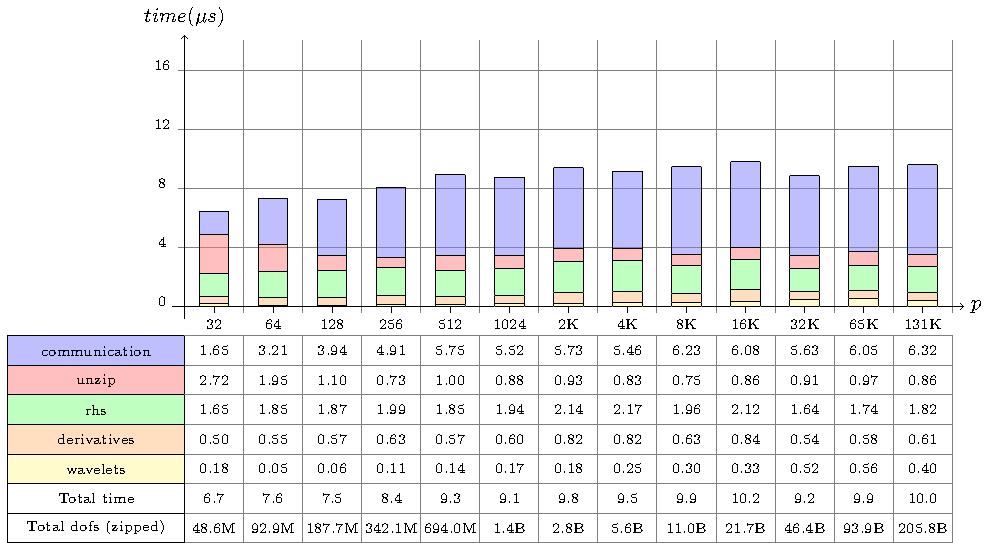
\includegraphics{plots/weak_r10}}}
		%\caption{\small Weak scaling results in ORNL's \Titan~for  $RK/(dof/p)$ (averaged over 10 steps) where $RK,dof,p$ denotes the time for single $RK$ step, degrees of freedom, and number of cores respectively,  with derivative computation (\texttt{deriv}), right hand side( {\texttt rhs}) computation, \texttt{unzip} cost, wavelet computation(\texttt{wavelets}) and communication cost (\texttt{comm}) with the approximate grain size of 1.536M unknowns where the number of cores ranging from $32$ to $131,072$ cores on $8192$ nodes where the largest problem having $206$ Billion unknowns.\label{fig:ws_g1000}}  % Above results are generated with mass ratio $\mu=10$ with \maxDepth~ 18 and wavelet tolerance of $10^{-6}$ 
		\vspace{-0.2in}
	\end{figure}	
	\Subhead{Weak scaling results}% (ORNL's \Titan~ upto $131K$ cores)} 

	\vspace{-0.5in}
	Weak scaling results in ORNL's \Titan~for  $RK/(dof/p)$ (averaged over 10 steps) where $RK,dof,p$ denotes the time for single $RK$ step, degrees of freedom, and number of cores respectively,  with derivative computation (\texttt{deriv}), right hand side( {\texttt rhs}) computation, \texttt{unzip} cost, wavelet computation(\texttt{wavelets}) and communication cost (\texttt{comm}) with the approximate grain size of 1.536M unknowns where the number of cores ranging from $32$ to $131,072$ cores on $8192$ nodes where the largest problem having $206$ Billion unknowns.
\end{textblock}
	

\begin{textblock}{10}(15,0)

\begin{figure}
		\centering
		\resizebox{!}{7\TPHorizModule}{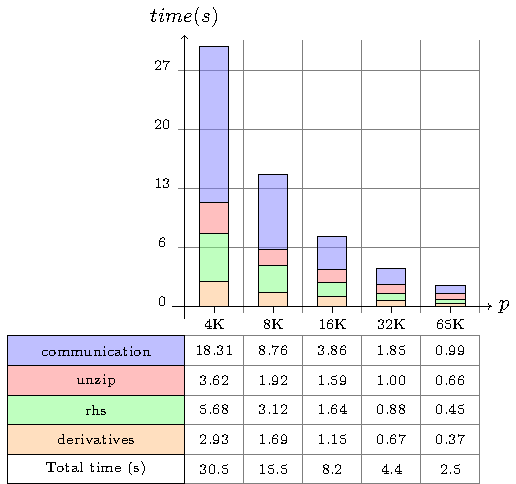
\includegraphics{plots/strong_r10}}
%		\caption{\small Strong scaling results in ORNL's \Titan~for a single RK step (averaged over 10 steps) with derivative computation (\texttt{deriv}), right hand side( {\texttt rhs}) computation, \texttt{unzip} cost and communication cost (\texttt{comm}) for a fixed problem size of $10.5B$ unknowns where the number of cores ranging from $4,096$ to $65,536$ cores on $4096$ nodes. Note that for strong scaling results re-meshing is disabled in order to keep the problem size fixed.  \label{fig:ss_r10} }
\end{figure}	
\Subhead{Strong scaling results}

Strong scaling results in ORNL's \Titan~for a single RK step (averaged over 10 steps) with derivative computation (\texttt{deriv}), right hand side( {\texttt rhs}) computation, \texttt{unzip} cost and communication cost (\texttt{comm}) for a fixed problem size of $10.5B$ unknowns where the number of cores ranging from $4,096$ to $65,536$ cores on $4096$ nodes. Note that for strong scaling results re-meshing is disabled in order to keep the problem size fixed.
\end{textblock}


%\begin{textblock}{9}(0,18)
%\Subhead{Octree adaptivity Vs. Block adaptivity}
%	\begin{figure}
%		\centering
%		\resizebox{!}{!}{
%		\begin{tikzpicture}
%		\begin{axis}[
%		%axis y line*=left,
%		ylabel={\small grid points $\rightarrow$},%ymax=1,
%		xlabel={\small mass ratio $\rightarrow$},legend pos=north west,
%		width=7in, height=2.5in
%		]
%		\addplot[thick,sq_b1,smooth,mark=*]  table [x={mr},y ={dof_zip}]{dat/stampede2/mr_et.dat};
%		\addplot[thick,sq_r1,smooth,mark=diamond*]  table [x={mr},y ={dof_zip}]{dat/stampede2/mr_dendro.dat};
%		\legend{\tiny ET(points), \tiny\dendro (points)}
%		\end{axis}
%		%	\begin{axis}[
%		%	axis y line*=right,%ymax=1.5e6,
%		%    axis x line=none,
%		%  ylabel={grid points $\rightarrow$},
%		%  width=0.45\textwidth, height=2in
%		%	]
%		%	\addplot[thick,sq_b3,smooth,mark=triangle*]  table [x={mr},y ={dof_zip}]{dat/stampede2/mr_et.dat};
%		%	\addplot[thick,sq_r3,smooth,mark=square*]  table [x={mr},y ={dof_zip}]{dat/stampede2/mr_dendro.dat};
%		%	\legend{ET(points), \dendro (points)}
%		%	\end{axis}
%		\end{tikzpicture} 
%		}
%		%\pgfplotstabletypeset[columns={mass ratio,points(ET),time(ET)(s),points(XXXX),time(XXXX)(s)}]{dat/stampede2/mr_dendro_et.dat}
%		\caption{\label{fig:et_avec_adaptivity} \small Comparison between \et~ and \dendrogr\ for number of spatial points with increasing mass ratios. Note that these are not from complete simulations and the size of the problem as well as the time per RK-step is likely to increase, but it illustrates the rate of increase for both approaches. Parameters for the above experiment generated such that total mass of black holes equals to $1$ and the separation distance is $32$ for all cases and \maxDepth~ is set in a way that the spatial discretization $dx<\frac{\min(m_1,m_2)}{16}$ where $m1,m2$ denotes the individual masses of black holes. 
%			%$RK$ time computed based average time to perform first $500$ time steps using $64$ cores on $2$ nodes in TACC's  \Stampede.
%			%\hs{I have updated the caption. }
%		}
%		\vspace{-0.2in}
%	\end{figure}
%\end{textblock}





\end{textblock}




%\begin{textblock}{7}(63,30)
%{\color{DarkBlue}\hrule}\medskip
%%	\Head{\NLSM:Simple Example}
%	
%%\begin{textblock}{6}(0,0)
%%
%%\Subhead{Single boosted block hole}
%%\begin{itemize}
%%	\item Single blak hole with unidirection momentum $P_i$. 
%%	\item Correct simulation should produce black hole moving in the $i^{th}$ direction(see figure \ref{fig:sbh_boost}). 
%%\end{itemize}
%%
%%\end{textblock}
%%
%%\begin{textblock}{6}(0,4)
%%\Subhead{NLSM: Non-linear sigma model}
%%\begin{equation*}
%%\chi_{tt}= \Delta \chi -\frac{\sin(2\chi)}{{\norm{x}_2}^2} 
%%\label{eq:nlsm}
%%\end{equation*}
%%we can rewrite the equation \ref{eq:nlsm} as 2 coupled PDEs first order in time and second order in space with a new scalar field $\phi$. 
%%\begin{align}
%%\phi_{t} &= \Delta \chi -\frac{\sin(2\chi)}{{\norm{x}_2}^2} \label{eq:phi} \\
%%\chi_{t} &= \phi \label{eq:chi} 
%%\end{align}
%%
%%The radiative boundary conditions are imposed as follows for each scalar field.
%%\begin{align}
%%\chi_{t} &= \frac{-x^t\nabla\chi - k(\chi-\chi_0)}{\norm{x}_2}, \\
%%\phi_{t} &= \frac{-x^t\nabla\phi - k(\phi-\phi_0)}{\norm{x}_2},
%%\end{align}
%%where $\chi_0$ and $\phi_0$ are the values at $\infty$.
%%\end{textblock}
%
%
%
%\end{textblock}

%\begin{textblock}{7}(70,30)
%	{\color{DarkBlue}\hrule}\medskip
%	\Head{Large mass ratio runs}
%	\vspace{0.5in}
%	\begin{figure}
%		\begin{subfigure}{0.33\textwidth}
%			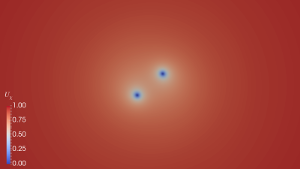
\includegraphics[width=0.9\textwidth]{figs/img_slice_chi_r1.png}
%			\caption{$q=1$}
%		\end{subfigure}
%		\begin{subfigure}{0.33\textwidth}
%			
\includegraphics[width=0.9\textwidth]{figs/img_slice_chi_r10.png}
%			\caption{$q=10$}
%		\end{subfigure}
%		\begin{subfigure}{0.33\textwidth}
%			
\includegraphics[width=0.9\textwidth]{figs/img_slice_chi_r100.png}
%			\caption{$q=100$}
%		\end{subfigure} \hfil
%		\begin{subfigure}{0.33\textwidth}
%			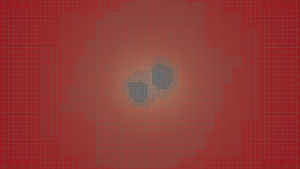
\includegraphics[width=0.9\textwidth]{figs/img_slice_level_r1.png}
%			\caption{$q=1$}
%		\end{subfigure}
%		\begin{subfigure}{0.33\textwidth}
%			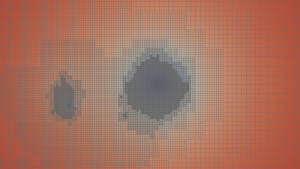
\includegraphics[width=0.9\textwidth]{figs/img_slice_level_r10.png}
%			\caption{$q=10$}
%		\end{subfigure}
%		\begin{subfigure}{0.33\textwidth}
%			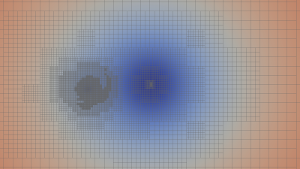
\includegraphics[width=0.9\textwidth]{figs/img_slice_level_r100.png}
%			\caption{$q=100$}
%		\end{subfigure}
%		\caption{\small Time step snapshots of the binary black hole problem of black hole mass ratios $1, 10 \& 100$ where we in the top row we plot the \BSSN~variable $\chi$ in the lower row we plot the WAMR grids for each case at that specific instance. \label{fig:large_q}}
%	\end{figure}
%	
%	
%\end{textblock}





% References <<<
  
%\begin{textblock}{7}(15.5,15.5) %<<<
%  {\color{DarkBlue}\hrule}
%  \hskip 1mm
%\end{textblock} %>>>


%% ================================================================

\begin{textblock}{62}(20,32)
{\color{DarkBlue}\hrule}\medskip
\Head{Binary compact mergers of different mass ratios}

\begin{textblock}{40}(0,0)
	\begin{figure}
		\begin{subfigure}{0.0714\textwidth}
			\centering
			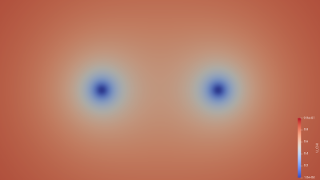
\includegraphics[height=1.5in]{figs/AE/r1/img_slice_000000.png}
			\caption{\small $\TT=0~M$}
		\end{subfigure}
		\begin{subfigure}{0.0714\textwidth}
			\centering
			
\includegraphics[height=1.5in]{figs/AE/r1/img_slice_000010.png}
			\caption{\small $\TT=19.5~M$}
		\end{subfigure}
		\begin{subfigure}{0.0714\textwidth}
			\centering
			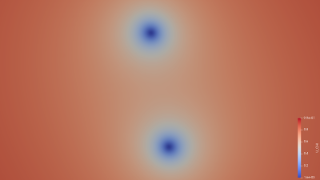
\includegraphics[height=1.5in]{figs/AE/r1/img_slice_000020.png}
			\caption{\small $\TT=39.0M$}
		\end{subfigure}
		\begin{subfigure}{0.0714\textwidth}
			\centering
			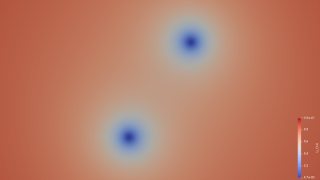
\includegraphics[height=1.5in]{figs/AE/r1/img_slice_000030.png}
			\caption{\small $\TT=58.5~M$}
		\end{subfigure}
		\begin{subfigure}{0.0714\textwidth}
			\centering
			
\includegraphics[height=1.5in]{figs/AE/r1/img_slice_000040.png}
			\caption{\small $\TT=78.0~M$}
		\end{subfigure}
		\begin{subfigure}{0.0714\textwidth}
			\centering
			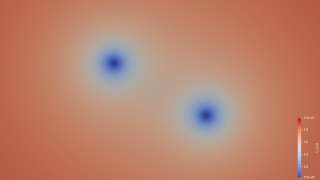
\includegraphics[height=1.5in]{figs/AE/r1/img_slice_000050.png}
			\caption{\small $\TT=97.5~M$}
		\end{subfigure}
		\begin{subfigure}{0.0714\textwidth}
			\centering
			
\includegraphics[height=1.5in]{figs/AE/r1/img_slice_000060.png}
			\caption{\small $\TT=117.0~M$}
		\end{subfigure}
		\begin{subfigure}{0.0714\textwidth}
			\centering
			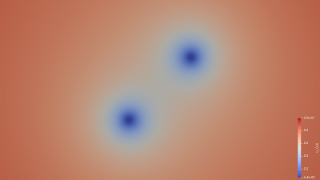
\includegraphics[height=1.5in]{figs/AE/r1/img_slice_000070.png}
			\caption{\small $\TT=136.5~M$}
		\end{subfigure}
		\begin{subfigure}{0.0714\textwidth}
			\centering
			
\includegraphics[height=1.5in]{figs/AE/r1/img_slice_000080.png}
			\caption{\small $\TT=156.0~M$}
		\end{subfigure}
		\begin{subfigure}{0.0714\textwidth}
			\centering
			
\includegraphics[height=1.5in]{figs/AE/r1/img_slice_000090.png}
			\caption{\small $\TT=175.5.0~M$}
		\end{subfigure}
		\begin{subfigure}{0.0714\textwidth}
			\centering
			
\includegraphics[height=1.5in]{figs/AE/r1/img_slice_000100.png}
			\caption{\small $\TT=195.0~M$}
		\end{subfigure}
		\begin{subfigure}{0.0714\textwidth}
			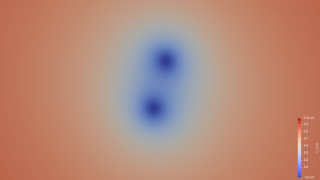
\includegraphics[height=1.5in]{figs/AE/r1/img_slice_000110.png}
			\caption{\small $\TT=214.5.0~M$}
		\end{subfigure}
		\begin{subfigure}{0.0714\textwidth}
			\centering
			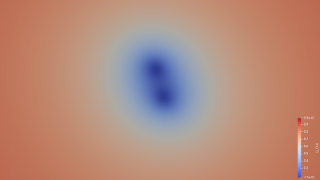
\includegraphics[height=1.5in]{figs/AE/r1/img_slice_000120.png}
			\caption{\small $\TT=234.0~M$}
		\end{subfigure}
		\begin{subfigure}{0.0714\textwidth}
			\centering
			
\includegraphics[height=1.5in]{figs/AE/r1/img_slice_000130.png}
			\caption{\small $\TT=253.5~M$}
		\end{subfigure}
	\caption{Slice of the \BSSN~ variable $\chi$ along the $z$-plane for equal mass ratio binary black holes. Above simulation performed in TACC's \Stampede~ using $1K$ cores with total simulation run time of $48hrs$ from the beginning to the merger event.  }
	\end{figure}
%	Slice of the \BSSN~ variable $\chi$ along the $z$-plane for equal mass ratio binary black holes. Above simulation performed in TACC's \Stampede~ using $1K$ cores with total simulation run time of $48hrs$ from the beginning to the merger event. 
\end{textblock}

\begin{textblock}{38}(0,3)
	\begin{figure}
		\begin{subfigure}{0.0714\textwidth}
			\centering
			
\includegraphics[height=1.5in]{figs/AE/r10/img_slice_000000.png}
			\caption{\small $\TT=0~M$}
		\end{subfigure}
		\begin{subfigure}{0.0714\textwidth}
			\centering
			\includegraphics[height=1.5in]{figs/AE/r10/img_slice_000010.png}
			\caption{\small $\TT=21.9~M$}
		\end{subfigure}
		\begin{subfigure}{0.0714\textwidth}
			\centering
			\includegraphics[height=1.5in]{figs/AE/r10/img_slice_000020.png}
			\caption{\small $\TT=43.9~M$}
		\end{subfigure}
		\begin{subfigure}{0.0714\textwidth}
			\centering
			\includegraphics[height=1.5in]{figs/AE/r10/img_slice_000030.png}
			\caption{\small $\TT=65.9~M$}
		\end{subfigure}
		\begin{subfigure}{0.0714\textwidth}
			\centering
			\includegraphics[height=1.5in]{figs/AE/r10/img_slice_000040.png}
			\caption{\small $\TT=87.8~M$}
		\end{subfigure}
		\begin{subfigure}{0.0714\textwidth}
			\centering
			\includegraphics[height=1.5in]{figs/AE/r10/img_slice_000050.png}
			\caption{\small $\TT=109.8~M$}
		\end{subfigure}
		\begin{subfigure}{0.0714\textwidth}
			\centering
			\includegraphics[height=1.5in]{figs/AE/r10/img_slice_000060.png}
			\caption{\small $\TT=131.8~M$}
		\end{subfigure}
		\begin{subfigure}{0.0714\textwidth}
			\centering
			\includegraphics[height=1.5in]{figs/AE/r10/img_slice_000070.png}
			\caption{\small $\TT=153.7~M$}
		\end{subfigure}
		\begin{subfigure}{0.0714\textwidth}
			\centering
			\includegraphics[height=1.5in]{figs/AE/r10/img_slice_000080.png}
			\caption{\small $\TT=175.7~M$}
		\end{subfigure}
		\begin{subfigure}{0.0714\textwidth}
			\centering
			\includegraphics[height=1.5in]{figs/AE/r10/img_slice_000090.png}
			\caption{\small $\TT=197.7~M$}
		\end{subfigure}
		\begin{subfigure}{0.0714\textwidth}
			\centering
			\includegraphics[height=1.5in]{figs/AE/r10/img_slice_000100.png}
			\caption{\small $\TT=219.7~M$}
		\end{subfigure}
		\caption{Slice of the \BSSN~ variable $\chi$ along the $z$-plane for mass ratio $q=10$ binary black holes.}
	\end{figure}
\end{textblock}

\begin{textblock}{38}(31,3)
	\begin{figure}
	\begin{subfigure}{0.0714\textwidth}
		\centering
		\includegraphics[height=1.5in]{figs/AE/r100/img_slice_000000.png}
		\caption{\small $\TT=0~M$}
	\end{subfigure}
	\begin{subfigure}{0.0714\textwidth}
		\centering
		\includegraphics[height=1.5in]{figs/AE/r100/img_slice_000020.png}
		\caption{\small $\TT=21.9~M$}
	\end{subfigure}
	\begin{subfigure}{0.0714\textwidth}
		\centering
		\includegraphics[height=1.5in]{figs/AE/r100/img_slice_000040.png}
		\caption{\small $\TT=43.9~M$}
	\end{subfigure}
	\begin{subfigure}{0.0714\textwidth}
		\centering
		\includegraphics[height=1.5in]{figs/AE/r100/img_slice_000060.png}
		\caption{\small $\TT=65.9~M$}
	\end{subfigure}
	\begin{subfigure}{0.0714\textwidth}
		\centering
		\includegraphics[height=1.5in]{figs/AE/r100/img_slice_000080.png}
		\caption{\small $\TT=87.8~M$}
	\end{subfigure}
	\begin{subfigure}{0.0714\textwidth}
		\centering
		\includegraphics[height=1.5in]{figs/AE/r100/img_slice_000100.png}
		\caption{\small $\TT=109.8~M$}
	\end{subfigure}
	\begin{subfigure}{0.0714\textwidth}
		\centering
		\includegraphics[height=1.5in]{figs/AE/r100/img_slice_000120.png}
		\caption{\small $\TT=131.8~M$}
	\end{subfigure}
	\begin{subfigure}{0.0714\textwidth}
		\centering
		\includegraphics[height=1.5in]{figs/AE/r100/img_slice_000140.png}
		\caption{\small $\TT=153.7~M$}
	\end{subfigure}
	\begin{subfigure}{0.0714\textwidth}
		\centering
		\includegraphics[height=1.5in]{figs/AE/r100/img_slice_000160.png}
		\caption{\small $\TT=175.7~M$}
	\end{subfigure}
	\begin{subfigure}{0.0714\textwidth}
		\centering
		\includegraphics[height=1.5in]{figs/AE/r100/img_slice_000180.png}
		\caption{\small $\TT=197.7~M$}
	\end{subfigure}
	\begin{subfigure}{0.0714\textwidth}
		\centering
		\includegraphics[height=1.5in]{figs/AE/r100/img_slice_000200.png}
		\caption{\small $\TT=219.7~M$}
	\end{subfigure}
	\caption{Slice of the \BSSN~ variable $\chi$ along the $z$-plane for mass ratio $q=100$ binary black holes.}
\end{figure}
\end{textblock}

%\begin{textblock}{22}(40,0)
%	\begin{figure}
%		
%			\begin{subfigure}{0.14\textwidth}
%			\centering
%			\includegraphics[height=1.5in]{figs/AE/sbh_boost/img_slice_000000.png}
%			\caption{\small $\TT=0~M$}
%		\end{subfigure}
%		\begin{subfigure}{0.14\textwidth}
%			\centering
%			\includegraphics[height=1.5in]{figs/AE/sbh_boost/img_slice_000050.png}
%			\caption{\small $\TT=21.9~M$}
%		\end{subfigure}
%		\begin{subfigure}{0.14\textwidth}
%			\centering
%			\includegraphics[height=1.5in]{figs/AE/sbh_boost/img_slice_000100.png}
%			\caption{\small $\TT=43.9~M$}
%		\end{subfigure}
%		\begin{subfigure}{0.14\textwidth}
%			\centering
%			\includegraphics[height=1.5in]{figs/AE/sbh_boost/img_slice_000150.png}
%			\caption{\small $\TT=65.9~M$}
%		\end{subfigure}
%		\begin{subfigure}{0.14\textwidth}
%			\centering
%			\includegraphics[height=1.5in]{figs/AE/sbh_boost/img_slice_000200.png}
%			\caption{\small $\TT=87.8~M$}
%		\end{subfigure}
%		\begin{subfigure}{0.14\textwidth}
%			\centering
%			\includegraphics[height=1.5in]{figs/AE/sbh_boost/img_slice_000250.png}
%			\caption{\small $\TT=109.8~M$}
%		\end{subfigure}
%		\begin{subfigure}{0.14\textwidth}
%			\centering
%			\includegraphics[height=1.5in]{figs/AE/sbh_boost/img_slice_000300.png}
%			\caption{\small $\TT=131.8~M$}
%		\end{subfigure}
%%		\begin{subfigure}{0.0714\textwidth}
%%			\centering
%%			\includegraphics[height=1.5in]{figs/AE/sbh_boost/img_slice_000350.png}
%%			\caption{\small $\TT=153.7~M$}
%%		\end{subfigure}
%%		\begin{subfigure}{0.0714\textwidth}
%%			\centering
%%			\includegraphics[height=1.5in]{figs/AE/sbh_boost/img_slice_000400.png}
%%			\caption{\small $\TT=175.7~M$}
%%		\end{subfigure}
%%		\begin{subfigure}{0.0714\textwidth}
%%			\centering
%%			\includegraphics[height=1.5in]{figs/AE/sbh_boost/img_slice_000450.png}
%%			\caption{\small $\TT=197.7~M$}
%%		\end{subfigure}
%%		\begin{subfigure}{0.0714\textwidth}
%%			\centering
%%			\includegraphics[height=1.5in]{figs/AE/sbh_boost/img_slice_000500.png}
%%			\caption{\small $\TT=219.7~M$}
%%		\end{subfigure}
%%		\begin{subfigure}{0.0714\textwidth}
%%			\centering
%%			\includegraphics[height=1.5in]{figs/AE/sbh_boost/img_slice_000550.png}
%%			\caption{\small $\TT=241.6~M$}
%%		\end{subfigure}
%%		\begin{subfigure}{0.0714\textwidth}
%%		\centering
%%		\includegraphics[height=1.5in]{figs/AE/sbh_boost/img_slice_000600.png}
%%		\caption{\small $\TT=219.7~M$}
%%		\end{subfigure}
%%	
%%		\begin{subfigure}{0.0714\textwidth}
%%		\centering
%%		\includegraphics[height=1.5in]{figs/AE/sbh_boost/img_slice_000649.png}
%%		\caption{\small $\TT=285.6~M$}
%%		\end{subfigure}
%		\caption{A single black hole boosted in the $x$-direction, with \maxDepth=12 and wavelet tolerance of $10^{-3}$. 
%			%Time is given in terms of the black hole mass, $M$.
%			\label{fig:sbh_boost}}
%	\end{figure}
%\end{textblock}
%	
%\begin{textblock}{22}(40,-0.7)
%\hfill\Head{ Accuracy of the code : Single boosted black hole}
%\end{textblock}	
	
\end{textblock}
  


%% =========================

%\begin{textblock}{6}(17,15.75) %<<<
%\resizebox{6\TPHorizModule}{!}{\includegraphics{figs/BottomRight}}
%\end{textblock} %>>>

\end{document}

